\documentclass[a4paper]{book}
\usepackage{a4wide}
\usepackage{makeidx}
\usepackage{graphicx}
\usepackage{multicol}
\usepackage{float}
\usepackage{listings}
\usepackage{color}
\usepackage{textcomp}
\usepackage{alltt}
\usepackage{times}
\usepackage{ifpdf}
\ifpdf
\usepackage[pdftex,
            pagebackref=true,
            colorlinks=true,
            linkcolor=blue,
            unicode
           ]{hyperref}
\else
\usepackage[ps2pdf,
            pagebackref=true,
            colorlinks=true,
            linkcolor=blue,
            unicode
           ]{hyperref}
\usepackage{pspicture}
\fi
\usepackage[utf8]{inputenc}
\usepackage{doxygen}
\lstset{language=C++,inputencoding=utf8,basicstyle=\footnotesize,breaklines=true,breakatwhitespace=true,tabsize=8,numbers=left }
\makeindex
\setcounter{tocdepth}{3}
\renewcommand{\footrulewidth}{0.4pt}
\begin{document}
\hypersetup{pageanchor=false}
\begin{titlepage}
\vspace*{7cm}
\begin{center}
{\Large SNPLASH }\\
\vspace*{1cm}
{\large Generated by Doxygen 1.6.3}\\
\vspace*{0.5cm}
{\small Wed Nov 30 21:15:27 2011}\\
\end{center}
\end{titlepage}
\clearemptydoublepage
\pagenumbering{roman}
\tableofcontents
\clearemptydoublepage
\pagenumbering{arabic}
\hypersetup{pageanchor=true}
\chapter{Todo List}
\label{todo}
\hypertarget{todo}{}
\label{todo__todo000001}
\hypertarget{todo__todo000001}{}
 
\begin{DoxyDescription}
\item[Global \hyperlink{classEngineParamReader_a0fcc8aa5dcc6a42dc88e94f7177d4322}{EngineParamReader::EngineParamReader}() ]Make all of these defaults for speed. 
\end{DoxyDescription}
\chapter{Deprecated List}
\label{deprecated}
\hypertarget{deprecated}{}
\label{deprecated__deprecated000001}
\hypertarget{deprecated__deprecated000001}{}
 
\begin{DoxyDescription}
\item[Global \hyperlink{classDandelion_a7d005ed3065f6d59bcdb569ac60a80d1}{Dandelion::computeHaplotypeTest}(\hyperlink{structDandelionHaploInfo}{DandelionHaploInfo} \&d) ]This is currently a simple chi2 test. Needs to be done with LR. This code is NOT tested and should never be included in production app.


\end{DoxyDescription}
\chapter{Bug List}
\label{bug}
\hypertarget{bug}{}
\label{bug__bug000001}
\hypertarget{bug__bug000001}{}
 
\begin{DoxyDescription}
\item[Global \hyperlink{classLinkageDisequilibrium_a11db054a2925bd82379a6b39a9f3464f}{LinkageDisequilibrium::dprimeOnPair}(int s1, int s2, \hyperlink{structLinkageMeasures}{LinkageMeasures} \&results) ]The error spits to cerr not logger. 
\end{DoxyDescription}

\label{bug__bug000002}
\hypertarget{bug__bug000002}{}
 
\begin{DoxyDescription}
\item[Global \hyperlink{namespacestrnutils_a68527d204971afac794cff1d78e3556f}{strnutils::spaced\_\-number}(double number, int numspaces, int precision, int buffer=0) ]Sometimes prints with too many spaces if a large exponent is involved. 
\end{DoxyDescription}

\label{bug__bug000003}
\hypertarget{bug__bug000003}{}
 
\begin{DoxyDescription}
\item[Global \hyperlink{classZaykin_a5afe5c8d000df0e1dce66d4a22891623}{Zaykin::runAllIndiv}(vector$<$ double $>$ \&testStats, vector$<$ int $>$ \&degsFreedom) ]This method not done yet. 
\end{DoxyDescription}
\chapter{Namespace Index}
\section{Namespace List}
Here is a list of all namespaces with brief descriptions:\begin{DoxyCompactList}
\item\contentsline{section}{\hyperlink{namespacestrnutils}{strnutils} }{\pageref{namespacestrnutils}}{}
\item\contentsline{section}{\hyperlink{namespacevecops}{vecops} }{\pageref{namespacevecops}}{}
\end{DoxyCompactList}

\chapter{Data Structure Index}
\section{Class Hierarchy}
This inheritance list is sorted roughly, but not completely, alphabetically:\begin{DoxyCompactList}
\item \contentsline{section}{AD\_\-Data}{\pageref{classAD__Data}}{}
\item \contentsline{section}{AD\_\-Rule}{\pageref{classAD__Rule}}{}
\item \contentsline{section}{ADTException}{\pageref{classADTException}}{}
\begin{DoxyCompactList}
\item \contentsline{section}{DataException}{\pageref{classDataException}}{}
\item \contentsline{section}{EMAlgorithmFailureException}{\pageref{classEMAlgorithmFailureException}}{}
\item \contentsline{section}{EMAlgorithmNoSetup}{\pageref{classEMAlgorithmNoSetup}}{}
\item \contentsline{section}{EMAlgorithmRunResultsMismatch}{\pageref{classEMAlgorithmRunResultsMismatch}}{}
\item \contentsline{section}{LinearRegressionException}{\pageref{classLinearRegressionException}}{}
\item \contentsline{section}{LogisticRegressionException}{\pageref{classLogisticRegressionException}}{}
\begin{DoxyCompactList}
\item \contentsline{section}{ConditionNumberEx}{\pageref{classConditionNumberEx}}{}
\item \contentsline{section}{DeterminantCalculationEx}{\pageref{classDeterminantCalculationEx}}{}
\item \contentsline{section}{InvalidNewRaphInputEx}{\pageref{classInvalidNewRaphInputEx}}{}
\item \contentsline{section}{MatrixNotSquareEx}{\pageref{classMatrixNotSquareEx}}{}
\item \contentsline{section}{NewtonRaphsonFailureEx}{\pageref{classNewtonRaphsonFailureEx}}{}
\item \contentsline{section}{NewtonRaphsonIterationEx}{\pageref{classNewtonRaphsonIterationEx}}{}
\item \contentsline{section}{SingularMatrixEx}{\pageref{classSingularMatrixEx}}{}
\end{DoxyCompactList}
\item \contentsline{section}{QSnpgwaException}{\pageref{classQSnpgwaException}}{}
\item \contentsline{section}{RunOrderException}{\pageref{classRunOrderException}}{}
\item \contentsline{section}{StatsException}{\pageref{classStatsException}}{}
\begin{DoxyCompactList}
\item \contentsline{section}{FDistributionException}{\pageref{classFDistributionException}}{}
\item \contentsline{section}{GammaFxnFailureException}{\pageref{classGammaFxnFailureException}}{}
\item \contentsline{section}{InvalidChiSquareException}{\pageref{classInvalidChiSquareException}}{}
\end{DoxyCompactList}
\end{DoxyCompactList}
\item \contentsline{section}{haplotype::alleleNumOutsideRangeEx}{\pageref{classhaplotype_1_1alleleNumOutsideRangeEx}}{}
\item \contentsline{section}{Condition}{\pageref{classCondition}}{}
\item \contentsline{section}{ContGenoStats}{\pageref{classContGenoStats}}{}
\item \contentsline{section}{ContGenoStatsResults}{\pageref{structContGenoStatsResults}}{}
\item \contentsline{section}{ContPopStats}{\pageref{classContPopStats}}{}
\item \contentsline{section}{ContPopStatsResults}{\pageref{structContPopStatsResults}}{}
\item \contentsline{section}{DandelionHaploInfo}{\pageref{structDandelionHaploInfo}}{}
\item \contentsline{section}{DandelionOutput}{\pageref{classDandelionOutput}}{}
\item \contentsline{section}{DandelionPProbInfo}{\pageref{structDandelionPProbInfo}}{}
\item \contentsline{section}{DandelionSnpInfo}{\pageref{structDandelionSnpInfo}}{}
\item \contentsline{section}{DataAccess}{\pageref{classDataAccess}}{}
\item \contentsline{section}{EM}{\pageref{classEM}}{}
\item \contentsline{section}{EMPersonalProbsResults}{\pageref{structEMPersonalProbsResults}}{}
\item \contentsline{section}{Engine}{\pageref{classEngine}}{}
\begin{DoxyCompactList}
\item \contentsline{section}{Classifies}{\pageref{classClassifies}}{}
\begin{DoxyCompactList}
\item \contentsline{section}{ADTree}{\pageref{classADTree}}{}
\item \contentsline{section}{Bagging}{\pageref{classBagging}}{}
\item \contentsline{section}{CrossValidation}{\pageref{classCrossValidation}}{}
\end{DoxyCompactList}
\item \contentsline{section}{Dandelion}{\pageref{classDandelion}}{}
\item \contentsline{section}{InterTwoLog}{\pageref{classInterTwoLog}}{}
\item \contentsline{section}{LinkageDisequilibrium}{\pageref{classLinkageDisequilibrium}}{}
\item \contentsline{section}{QSnpgwa}{\pageref{classQSnpgwa}}{}
\item \contentsline{section}{Snpgwa}{\pageref{classSnpgwa}}{}
\end{DoxyCompactList}
\item \contentsline{section}{EngineParamReader}{\pageref{classEngineParamReader}}{}
\item \contentsline{section}{GenoStats}{\pageref{classGenoStats}}{}
\item \contentsline{section}{GenoStatsResults}{\pageref{structGenoStatsResults}}{}
\item \contentsline{section}{HaploStats}{\pageref{classHaploStats}}{}
\item \contentsline{section}{HaploStatsResults}{\pageref{structHaploStatsResults}}{}
\item \contentsline{section}{haplotype}{\pageref{classhaplotype}}{}
\item \contentsline{section}{InterTwoLogMeasures}{\pageref{structInterTwoLogMeasures}}{}
\item \contentsline{section}{InterTwoLogOutput}{\pageref{classInterTwoLogOutput}}{}
\item \contentsline{section}{LinearRegression}{\pageref{classLinearRegression}}{}
\item \contentsline{section}{LinkageMeasures}{\pageref{structLinkageMeasures}}{}
\item \contentsline{section}{LinkageOutput}{\pageref{classLinkageOutput}}{}
\item \contentsline{section}{LinRegStats}{\pageref{structLinRegStats}}{}
\item \contentsline{section}{Logger}{\pageref{classLogger}}{}
\item \contentsline{section}{LogisticRegression}{\pageref{classLogisticRegression}}{}
\item \contentsline{section}{SnpData::MapData}{\pageref{structSnpData_1_1MapData}}{}
\item \contentsline{section}{MapData}{\pageref{structMapData}}{}
\item \contentsline{section}{Output}{\pageref{classOutput}}{}
\item \contentsline{section}{ParamReader}{\pageref{classParamReader}}{}
\item \contentsline{section}{PopStats}{\pageref{classPopStats}}{}
\item \contentsline{section}{PopStatsResults}{\pageref{structPopStatsResults}}{}
\item \contentsline{section}{Precondition}{\pageref{classPrecondition}}{}
\item \contentsline{section}{QSnpgwaOutput}{\pageref{classQSnpgwaOutput}}{}
\item \contentsline{section}{RandWH}{\pageref{classRandWH}}{}
\item \contentsline{section}{Reader}{\pageref{classReader}}{}
\begin{DoxyCompactList}
\item \contentsline{section}{ArffReader}{\pageref{classArffReader}}{}
\item \contentsline{section}{BinaryBedReader}{\pageref{classBinaryBedReader}}{}
\item \contentsline{section}{LinkageReader}{\pageref{classLinkageReader}}{}
\end{DoxyCompactList}
\item \contentsline{section}{SnpData}{\pageref{classSnpData}}{}
\item \contentsline{section}{SnpgwaOutput}{\pageref{classSnpgwaOutput}}{}
\item \contentsline{section}{SnpInfo}{\pageref{classSnpInfo}}{}
\item \contentsline{section}{Statistics}{\pageref{classStatistics}}{}
\item \contentsline{section}{ContGenoStats::statisticsOutput}{\pageref{structContGenoStats_1_1statisticsOutput}}{}
\item \contentsline{section}{StatsFillable}{\pageref{classStatsFillable}}{}
\begin{DoxyCompactList}
\item \contentsline{section}{LRStats}{\pageref{classLRStats}}{}
\item \contentsline{section}{ZaykinGlobalStatsResults}{\pageref{classZaykinGlobalStatsResults}}{}
\item \contentsline{section}{ZaykinStatsInfo}{\pageref{classZaykinStatsInfo}}{}
\end{DoxyCompactList}
\item \contentsline{section}{Zaykin}{\pageref{classZaykin}}{}
\end{DoxyCompactList}

\chapter{Data Structure Index}
\section{Data Structures}
Here are the data structures with brief descriptions:\begin{DoxyCompactList}
\item\contentsline{section}{\hyperlink{classAD__Data}{AD\_\-Data} }{\pageref{classAD__Data}}{}
\item\contentsline{section}{\hyperlink{classAD__Rule}{AD\_\-Rule} }{\pageref{classAD__Rule}}{}
\item\contentsline{section}{\hyperlink{classADTException}{ADTException} }{\pageref{classADTException}}{}
\item\contentsline{section}{\hyperlink{classADTree}{ADTree} }{\pageref{classADTree}}{}
\item\contentsline{section}{\hyperlink{classhaplotype_1_1alleleNumOutsideRangeEx}{haplotype::alleleNumOutsideRangeEx} }{\pageref{classhaplotype_1_1alleleNumOutsideRangeEx}}{}
\item\contentsline{section}{\hyperlink{classArffReader}{ArffReader} }{\pageref{classArffReader}}{}
\item\contentsline{section}{\hyperlink{classBagging}{Bagging} }{\pageref{classBagging}}{}
\item\contentsline{section}{\hyperlink{classBinaryBedReader}{BinaryBedReader} }{\pageref{classBinaryBedReader}}{}
\item\contentsline{section}{\hyperlink{classClassifies}{Classifies} }{\pageref{classClassifies}}{}
\item\contentsline{section}{\hyperlink{classCondition}{Condition} }{\pageref{classCondition}}{}
\item\contentsline{section}{\hyperlink{classConditionNumberEx}{ConditionNumberEx} }{\pageref{classConditionNumberEx}}{}
\item\contentsline{section}{\hyperlink{classContGenoStats}{ContGenoStats} }{\pageref{classContGenoStats}}{}
\item\contentsline{section}{\hyperlink{structContGenoStatsResults}{ContGenoStatsResults} }{\pageref{structContGenoStatsResults}}{}
\item\contentsline{section}{\hyperlink{classContPopStats}{ContPopStats} }{\pageref{classContPopStats}}{}
\item\contentsline{section}{\hyperlink{structContPopStatsResults}{ContPopStatsResults} }{\pageref{structContPopStatsResults}}{}
\item\contentsline{section}{\hyperlink{classCrossValidation}{CrossValidation} }{\pageref{classCrossValidation}}{}
\item\contentsline{section}{\hyperlink{classDandelion}{Dandelion} }{\pageref{classDandelion}}{}
\item\contentsline{section}{\hyperlink{structDandelionHaploInfo}{DandelionHaploInfo} }{\pageref{structDandelionHaploInfo}}{}
\item\contentsline{section}{\hyperlink{classDandelionOutput}{DandelionOutput} }{\pageref{classDandelionOutput}}{}
\item\contentsline{section}{\hyperlink{structDandelionPProbInfo}{DandelionPProbInfo} }{\pageref{structDandelionPProbInfo}}{}
\item\contentsline{section}{\hyperlink{structDandelionSnpInfo}{DandelionSnpInfo} }{\pageref{structDandelionSnpInfo}}{}
\item\contentsline{section}{\hyperlink{classDataAccess}{DataAccess} }{\pageref{classDataAccess}}{}
\item\contentsline{section}{\hyperlink{classDataException}{DataException} }{\pageref{classDataException}}{}
\item\contentsline{section}{\hyperlink{classDeterminantCalculationEx}{DeterminantCalculationEx} }{\pageref{classDeterminantCalculationEx}}{}
\item\contentsline{section}{\hyperlink{classEM}{EM} }{\pageref{classEM}}{}
\item\contentsline{section}{\hyperlink{classEMAlgorithmFailureException}{EMAlgorithmFailureException} }{\pageref{classEMAlgorithmFailureException}}{}
\item\contentsline{section}{\hyperlink{classEMAlgorithmNoSetup}{EMAlgorithmNoSetup} }{\pageref{classEMAlgorithmNoSetup}}{}
\item\contentsline{section}{\hyperlink{classEMAlgorithmRunResultsMismatch}{EMAlgorithmRunResultsMismatch} }{\pageref{classEMAlgorithmRunResultsMismatch}}{}
\item\contentsline{section}{\hyperlink{structEMPersonalProbsResults}{EMPersonalProbsResults} }{\pageref{structEMPersonalProbsResults}}{}
\item\contentsline{section}{\hyperlink{classEngine}{Engine} }{\pageref{classEngine}}{}
\item\contentsline{section}{\hyperlink{classEngineParamReader}{EngineParamReader} }{\pageref{classEngineParamReader}}{}
\item\contentsline{section}{\hyperlink{classFDistributionException}{FDistributionException} }{\pageref{classFDistributionException}}{}
\item\contentsline{section}{\hyperlink{classGammaFxnFailureException}{GammaFxnFailureException} }{\pageref{classGammaFxnFailureException}}{}
\item\contentsline{section}{\hyperlink{classGenoStats}{GenoStats} }{\pageref{classGenoStats}}{}
\item\contentsline{section}{\hyperlink{structGenoStatsResults}{GenoStatsResults} }{\pageref{structGenoStatsResults}}{}
\item\contentsline{section}{\hyperlink{classHaploStats}{HaploStats} }{\pageref{classHaploStats}}{}
\item\contentsline{section}{\hyperlink{structHaploStatsResults}{HaploStatsResults} }{\pageref{structHaploStatsResults}}{}
\item\contentsline{section}{\hyperlink{classhaplotype}{haplotype} }{\pageref{classhaplotype}}{}
\item\contentsline{section}{\hyperlink{classInterTwoLog}{InterTwoLog} }{\pageref{classInterTwoLog}}{}
\item\contentsline{section}{\hyperlink{structInterTwoLogMeasures}{InterTwoLogMeasures} }{\pageref{structInterTwoLogMeasures}}{}
\item\contentsline{section}{\hyperlink{classInterTwoLogOutput}{InterTwoLogOutput} }{\pageref{classInterTwoLogOutput}}{}
\item\contentsline{section}{\hyperlink{classInvalidChiSquareException}{InvalidChiSquareException} }{\pageref{classInvalidChiSquareException}}{}
\item\contentsline{section}{\hyperlink{classInvalidNewRaphInputEx}{InvalidNewRaphInputEx} }{\pageref{classInvalidNewRaphInputEx}}{}
\item\contentsline{section}{\hyperlink{classLinearRegression}{LinearRegression} }{\pageref{classLinearRegression}}{}
\item\contentsline{section}{\hyperlink{classLinearRegressionException}{LinearRegressionException} }{\pageref{classLinearRegressionException}}{}
\item\contentsline{section}{\hyperlink{classLinkageDisequilibrium}{LinkageDisequilibrium} }{\pageref{classLinkageDisequilibrium}}{}
\item\contentsline{section}{\hyperlink{structLinkageMeasures}{LinkageMeasures} }{\pageref{structLinkageMeasures}}{}
\item\contentsline{section}{\hyperlink{classLinkageOutput}{LinkageOutput} }{\pageref{classLinkageOutput}}{}
\item\contentsline{section}{\hyperlink{classLinkageReader}{LinkageReader} }{\pageref{classLinkageReader}}{}
\item\contentsline{section}{\hyperlink{structLinRegStats}{LinRegStats} }{\pageref{structLinRegStats}}{}
\item\contentsline{section}{\hyperlink{classLogger}{Logger} }{\pageref{classLogger}}{}
\item\contentsline{section}{\hyperlink{classLogisticRegression}{LogisticRegression} }{\pageref{classLogisticRegression}}{}
\item\contentsline{section}{\hyperlink{classLogisticRegressionException}{LogisticRegressionException} }{\pageref{classLogisticRegressionException}}{}
\item\contentsline{section}{\hyperlink{classLRStats}{LRStats} }{\pageref{classLRStats}}{}
\item\contentsline{section}{\hyperlink{structSnpData_1_1MapData}{SnpData::MapData} }{\pageref{structSnpData_1_1MapData}}{}
\item\contentsline{section}{\hyperlink{structMapData}{MapData} }{\pageref{structMapData}}{}
\item\contentsline{section}{\hyperlink{classMatrixNotSquareEx}{MatrixNotSquareEx} }{\pageref{classMatrixNotSquareEx}}{}
\item\contentsline{section}{\hyperlink{classNewtonRaphsonFailureEx}{NewtonRaphsonFailureEx} }{\pageref{classNewtonRaphsonFailureEx}}{}
\item\contentsline{section}{\hyperlink{classNewtonRaphsonIterationEx}{NewtonRaphsonIterationEx} }{\pageref{classNewtonRaphsonIterationEx}}{}
\item\contentsline{section}{\hyperlink{classOutput}{Output} }{\pageref{classOutput}}{}
\item\contentsline{section}{\hyperlink{classParamReader}{ParamReader} }{\pageref{classParamReader}}{}
\item\contentsline{section}{\hyperlink{classPopStats}{PopStats} }{\pageref{classPopStats}}{}
\item\contentsline{section}{\hyperlink{structPopStatsResults}{PopStatsResults} }{\pageref{structPopStatsResults}}{}
\item\contentsline{section}{\hyperlink{classPrecondition}{Precondition} }{\pageref{classPrecondition}}{}
\item\contentsline{section}{\hyperlink{classQSnpgwa}{QSnpgwa} }{\pageref{classQSnpgwa}}{}
\item\contentsline{section}{\hyperlink{classQSnpgwaException}{QSnpgwaException} }{\pageref{classQSnpgwaException}}{}
\item\contentsline{section}{\hyperlink{classQSnpgwaOutput}{QSnpgwaOutput} }{\pageref{classQSnpgwaOutput}}{}
\item\contentsline{section}{\hyperlink{classRandWH}{RandWH} }{\pageref{classRandWH}}{}
\item\contentsline{section}{\hyperlink{classReader}{Reader} }{\pageref{classReader}}{}
\item\contentsline{section}{\hyperlink{classRunOrderException}{RunOrderException} }{\pageref{classRunOrderException}}{}
\item\contentsline{section}{\hyperlink{classSingularMatrixEx}{SingularMatrixEx} }{\pageref{classSingularMatrixEx}}{}
\item\contentsline{section}{\hyperlink{classSnpData}{SnpData} }{\pageref{classSnpData}}{}
\item\contentsline{section}{\hyperlink{classSnpgwa}{Snpgwa} }{\pageref{classSnpgwa}}{}
\item\contentsline{section}{\hyperlink{classSnpgwaOutput}{SnpgwaOutput} }{\pageref{classSnpgwaOutput}}{}
\item\contentsline{section}{\hyperlink{classSnpInfo}{SnpInfo} }{\pageref{classSnpInfo}}{}
\item\contentsline{section}{\hyperlink{classStatistics}{Statistics} }{\pageref{classStatistics}}{}
\item\contentsline{section}{\hyperlink{structContGenoStats_1_1statisticsOutput}{ContGenoStats::statisticsOutput} }{\pageref{structContGenoStats_1_1statisticsOutput}}{}
\item\contentsline{section}{\hyperlink{classStatsException}{StatsException} }{\pageref{classStatsException}}{}
\item\contentsline{section}{\hyperlink{classStatsFillable}{StatsFillable} }{\pageref{classStatsFillable}}{}
\item\contentsline{section}{\hyperlink{classZaykin}{Zaykin} }{\pageref{classZaykin}}{}
\item\contentsline{section}{\hyperlink{classZaykinGlobalStatsResults}{ZaykinGlobalStatsResults} }{\pageref{classZaykinGlobalStatsResults}}{}
\item\contentsline{section}{\hyperlink{classZaykinStatsInfo}{ZaykinStatsInfo} }{\pageref{classZaykinStatsInfo}}{}
\end{DoxyCompactList}

\chapter{File Index}
\section{File List}
Here is a list of all files with brief descriptions:\begin{DoxyCompactList}
\item\contentsline{section}{\hyperlink{Makefile_8inc}{Makefile.inc} }{\pageref{Makefile_8inc}}{}
\item\contentsline{section}{\hyperlink{snpadt_8cpp}{snpadt.cpp} }{\pageref{snpadt_8cpp}}{}
\item\contentsline{section}{engine/\hyperlink{combinable_8h}{combinable.h} }{\pageref{combinable_8h}}{}
\item\contentsline{section}{engine/\hyperlink{data__plugin_8cpp}{data\_\-plugin.cpp} }{\pageref{data__plugin_8cpp}}{}
\item\contentsline{section}{engine/\hyperlink{data__plugin_8h}{data\_\-plugin.h} }{\pageref{data__plugin_8h}}{}
\item\contentsline{section}{engine/\hyperlink{engine_8h}{engine.h} }{\pageref{engine_8h}}{}
\item\contentsline{section}{engine/\hyperlink{randwh_8cpp}{randwh.cpp} }{\pageref{randwh_8cpp}}{}
\item\contentsline{section}{engine/\hyperlink{randwh_8h}{randwh.h} }{\pageref{randwh_8h}}{}
\item\contentsline{section}{engine/\hyperlink{snp__data_8cpp}{snp\_\-data.cpp} }{\pageref{snp__data_8cpp}}{}
\item\contentsline{section}{engine/\hyperlink{snp__data_8hh}{snp\_\-data.hh} }{\pageref{snp__data_8hh}}{}
\item\contentsline{section}{engine/adtree/\hyperlink{ad__rule_8cpp}{ad\_\-rule.cpp} }{\pageref{ad__rule_8cpp}}{}
\item\contentsline{section}{engine/adtree/\hyperlink{ad__rule_8h}{ad\_\-rule.h} }{\pageref{ad__rule_8h}}{}
\item\contentsline{section}{engine/adtree/\hyperlink{ad__tree__data_8cpp}{ad\_\-tree\_\-data.cpp} }{\pageref{ad__tree__data_8cpp}}{}
\item\contentsline{section}{engine/adtree/\hyperlink{ad__tree__data_8h}{ad\_\-tree\_\-data.h} }{\pageref{ad__tree__data_8h}}{}
\item\contentsline{section}{engine/adtree/\hyperlink{adtree_8cpp}{adtree.cpp} }{\pageref{adtree_8cpp}}{}
\item\contentsline{section}{engine/adtree/\hyperlink{adtree_8h}{adtree.h} }{\pageref{adtree_8h}}{}
\item\contentsline{section}{engine/adtree/\hyperlink{condition_8cpp}{condition.cpp} }{\pageref{condition_8cpp}}{}
\item\contentsline{section}{engine/adtree/\hyperlink{condition_8h}{condition.h} }{\pageref{condition_8h}}{}
\item\contentsline{section}{engine/adtree/\hyperlink{precondition_8cpp}{precondition.cpp} }{\pageref{precondition_8cpp}}{}
\item\contentsline{section}{engine/adtree/\hyperlink{precondition_8h}{precondition.h} }{\pageref{precondition_8h}}{}
\item\contentsline{section}{engine/bagging/\hyperlink{bagging_8cpp}{bagging.cpp} }{\pageref{bagging_8cpp}}{}
\item\contentsline{section}{engine/bagging/\hyperlink{bagging_8h}{bagging.h} }{\pageref{bagging_8h}}{}
\item\contentsline{section}{engine/crossval/\hyperlink{cross__val_8cpp}{cross\_\-val.cpp} }{\pageref{cross__val_8cpp}}{}
\item\contentsline{section}{engine/crossval/\hyperlink{cross__val_8h}{cross\_\-val.h} }{\pageref{cross__val_8h}}{}
\item\contentsline{section}{engine/dandelion/\hyperlink{dandelion_8cpp}{dandelion.cpp} }{\pageref{dandelion_8cpp}}{}
\item\contentsline{section}{engine/dandelion/\hyperlink{dandelion_8hh}{dandelion.hh} }{\pageref{dandelion_8hh}}{}
\item\contentsline{section}{engine/em/\hyperlink{em_8cpp}{em.cpp} }{\pageref{em_8cpp}}{}
\item\contentsline{section}{engine/em/\hyperlink{em_8h}{em.h} }{\pageref{em_8h}}{}
\item\contentsline{section}{engine/em/\hyperlink{haplotype_8cpp}{haplotype.cpp} }{\pageref{haplotype_8cpp}}{}
\item\contentsline{section}{engine/em/\hyperlink{haplotype_8h}{haplotype.h} }{\pageref{haplotype_8h}}{}
\item\contentsline{section}{engine/intertwolog/\hyperlink{intertwolog_8cpp}{intertwolog.cpp} }{\pageref{intertwolog_8cpp}}{}
\item\contentsline{section}{engine/intertwolog/\hyperlink{intertwolog_8hh}{intertwolog.hh} }{\pageref{intertwolog_8hh}}{}
\item\contentsline{section}{engine/ld/\hyperlink{ld_8cpp}{ld.cpp} }{\pageref{ld_8cpp}}{}
\item\contentsline{section}{engine/ld/\hyperlink{ld_8h}{ld.h} }{\pageref{ld_8h}}{}
\item\contentsline{section}{engine/output/\hyperlink{dandelion__out_8cpp}{dandelion\_\-out.cpp} }{\pageref{dandelion__out_8cpp}}{}
\item\contentsline{section}{engine/output/\hyperlink{dandelion__out_8hh}{dandelion\_\-out.hh} }{\pageref{dandelion__out_8hh}}{}
\item\contentsline{section}{engine/output/\hyperlink{dprime__out_8cpp}{dprime\_\-out.cpp} }{\pageref{dprime__out_8cpp}}{}
\item\contentsline{section}{engine/output/\hyperlink{dprime__out_8h}{dprime\_\-out.h} }{\pageref{dprime__out_8h}}{}
\item\contentsline{section}{engine/output/\hyperlink{intertwolog__out_8cpp}{intertwolog\_\-out.cpp} }{\pageref{intertwolog__out_8cpp}}{}
\item\contentsline{section}{engine/output/\hyperlink{intertwolog__out_8hh}{intertwolog\_\-out.hh} }{\pageref{intertwolog__out_8hh}}{}
\item\contentsline{section}{engine/output/\hyperlink{output_8cpp}{output.cpp} }{\pageref{output_8cpp}}{}
\item\contentsline{section}{engine/output/\hyperlink{output_8h}{output.h} }{\pageref{output_8h}}{}
\item\contentsline{section}{engine/output/\hyperlink{qsnpgwa__out_8cpp}{qsnpgwa\_\-out.cpp} }{\pageref{qsnpgwa__out_8cpp}}{}
\item\contentsline{section}{engine/output/\hyperlink{qsnpgwa__out_8hh}{qsnpgwa\_\-out.hh} }{\pageref{qsnpgwa__out_8hh}}{}
\item\contentsline{section}{engine/output/\hyperlink{snpgwa__out_8cpp}{snpgwa\_\-out.cpp} }{\pageref{snpgwa__out_8cpp}}{}
\item\contentsline{section}{engine/output/\hyperlink{snpgwa__out_8hh}{snpgwa\_\-out.hh} }{\pageref{snpgwa__out_8hh}}{}
\item\contentsline{section}{engine/output/\hyperlink{snpinfo__out_8cpp}{snpinfo\_\-out.cpp} }{\pageref{snpinfo__out_8cpp}}{}
\item\contentsline{section}{engine/output/\hyperlink{snpinfo__out_8hh}{snpinfo\_\-out.hh} }{\pageref{snpinfo__out_8hh}}{}
\item\contentsline{section}{engine/qsnpgwa/\hyperlink{cont__genostats_8cpp}{cont\_\-genostats.cpp} }{\pageref{cont__genostats_8cpp}}{}
\item\contentsline{section}{engine/qsnpgwa/\hyperlink{cont__genostats_8hh}{cont\_\-genostats.hh} }{\pageref{cont__genostats_8hh}}{}
\item\contentsline{section}{engine/qsnpgwa/\hyperlink{cont__popstats_8cpp}{cont\_\-popstats.cpp} }{\pageref{cont__popstats_8cpp}}{}
\item\contentsline{section}{engine/qsnpgwa/\hyperlink{cont__popstats_8hh}{cont\_\-popstats.hh} }{\pageref{cont__popstats_8hh}}{}
\item\contentsline{section}{engine/qsnpgwa/\hyperlink{qsnpgwa_8cpp}{qsnpgwa.cpp} }{\pageref{qsnpgwa_8cpp}}{}
\item\contentsline{section}{engine/qsnpgwa/\hyperlink{qsnpgwa_8hh}{qsnpgwa.hh} }{\pageref{qsnpgwa_8hh}}{}
\item\contentsline{section}{engine/snpgwa/\hyperlink{genostats_8cpp}{genostats.cpp} }{\pageref{genostats_8cpp}}{}
\item\contentsline{section}{engine/snpgwa/\hyperlink{genostats_8hh}{genostats.hh} }{\pageref{genostats_8hh}}{}
\item\contentsline{section}{engine/snpgwa/\hyperlink{haplostats_8cpp}{haplostats.cpp} }{\pageref{haplostats_8cpp}}{}
\item\contentsline{section}{engine/snpgwa/\hyperlink{haplostats_8hh}{haplostats.hh} }{\pageref{haplostats_8hh}}{}
\item\contentsline{section}{engine/snpgwa/\hyperlink{popstats_8cpp}{popstats.cpp} }{\pageref{popstats_8cpp}}{}
\item\contentsline{section}{engine/snpgwa/\hyperlink{popstats_8hh}{popstats.hh} }{\pageref{popstats_8hh}}{}
\item\contentsline{section}{engine/snpgwa/\hyperlink{snpgwa_8cpp}{snpgwa.cpp} }{\pageref{snpgwa_8cpp}}{}
\item\contentsline{section}{engine/snpgwa/\hyperlink{snpgwa_8h}{snpgwa.h} }{\pageref{snpgwa_8h}}{}
\item\contentsline{section}{engine/utils/\hyperlink{exceptions_8h}{exceptions.h} }{\pageref{exceptions_8h}}{}
\item\contentsline{section}{engine/utils/\hyperlink{float__ops_8cpp}{float\_\-ops.cpp} }{\pageref{float__ops_8cpp}}{}
\item\contentsline{section}{engine/utils/\hyperlink{float__ops_8hh}{float\_\-ops.hh} }{\pageref{float__ops_8hh}}{}
\item\contentsline{section}{engine/utils/\hyperlink{linear__regression_8cpp}{linear\_\-regression.cpp} }{\pageref{linear__regression_8cpp}}{}
\item\contentsline{section}{engine/utils/\hyperlink{linear__regression_8hh}{linear\_\-regression.hh} }{\pageref{linear__regression_8hh}}{}
\item\contentsline{section}{engine/utils/\hyperlink{lr_8cpp}{lr.cpp} }{\pageref{lr_8cpp}}{}
\item\contentsline{section}{engine/utils/\hyperlink{lr_8hh}{lr.hh} }{\pageref{lr_8hh}}{}
\item\contentsline{section}{engine/utils/\hyperlink{statistics_8cpp}{statistics.cpp} }{\pageref{statistics_8cpp}}{}
\item\contentsline{section}{engine/utils/\hyperlink{statistics_8h}{statistics.h} }{\pageref{statistics_8h}}{}
\item\contentsline{section}{engine/utils/\hyperlink{stringutils_8cpp}{stringutils.cpp} }{\pageref{stringutils_8cpp}}{}
\item\contentsline{section}{engine/utils/\hyperlink{stringutils_8h}{stringutils.h} }{\pageref{stringutils_8h}}{}
\item\contentsline{section}{engine/utils/\hyperlink{vecops_8cpp}{vecops.cpp} }{\pageref{vecops_8cpp}}{}
\item\contentsline{section}{engine/utils/\hyperlink{vecops_8hh}{vecops.hh} }{\pageref{vecops_8hh}}{}
\item\contentsline{section}{engine/utils/\hyperlink{zaykin_8cpp}{zaykin.cpp} }{\pageref{zaykin_8cpp}}{}
\item\contentsline{section}{engine/utils/\hyperlink{zaykin_8hh}{zaykin.hh} }{\pageref{zaykin_8hh}}{}
\item\contentsline{section}{logger/\hyperlink{log_8cpp}{log.cpp} }{\pageref{log_8cpp}}{}
\item\contentsline{section}{logger/\hyperlink{log_8hh}{log.hh} }{\pageref{log_8hh}}{}
\item\contentsline{section}{param/\hyperlink{engine__param__reader_8cpp}{engine\_\-param\_\-reader.cpp} }{\pageref{engine__param__reader_8cpp}}{}
\item\contentsline{section}{param/\hyperlink{engine__param__reader_8h}{engine\_\-param\_\-reader.h} }{\pageref{engine__param__reader_8h}}{}
\item\contentsline{section}{param/\hyperlink{param__reader_8cpp}{param\_\-reader.cpp} }{\pageref{param__reader_8cpp}}{}
\item\contentsline{section}{param/\hyperlink{param__reader_8h}{param\_\-reader.h} }{\pageref{param__reader_8h}}{}
\item\contentsline{section}{reader/\hyperlink{arff__reader_8cpp}{arff\_\-reader.cpp} }{\pageref{arff__reader_8cpp}}{}
\item\contentsline{section}{reader/\hyperlink{arff__reader_8h}{arff\_\-reader.h} }{\pageref{arff__reader_8h}}{}
\item\contentsline{section}{reader/\hyperlink{binary__bed__reader_8cpp}{binary\_\-bed\_\-reader.cpp} }{\pageref{binary__bed__reader_8cpp}}{}
\item\contentsline{section}{reader/\hyperlink{binary__bed__reader_8h}{binary\_\-bed\_\-reader.h} }{\pageref{binary__bed__reader_8h}}{}
\item\contentsline{section}{reader/\hyperlink{linkage__reader_8cpp}{linkage\_\-reader.cpp} }{\pageref{linkage__reader_8cpp}}{}
\item\contentsline{section}{reader/\hyperlink{linkage__reader_8h}{linkage\_\-reader.h} }{\pageref{linkage__reader_8h}}{}
\item\contentsline{section}{reader/\hyperlink{reader_8cpp}{reader.cpp} }{\pageref{reader_8cpp}}{}
\item\contentsline{section}{reader/\hyperlink{reader_8h}{reader.h} }{\pageref{reader_8h}}{}
\item\contentsline{section}{unittest/engine/utils/\hyperlink{test__lr__engine_8cpp}{test\_\-lr\_\-engine.cpp} }{\pageref{test__lr__engine_8cpp}}{}
\item\contentsline{section}{unittest/param/\hyperlink{test__engine__params_8cpp}{test\_\-engine\_\-params.cpp} }{\pageref{test__engine__params_8cpp}}{}
\end{DoxyCompactList}

\chapter{Namespace Documentation}
\hypertarget{namespacestrnutils}{
\section{strnutils Namespace Reference}
\label{namespacestrnutils}\index{strnutils@{strnutils}}
}
\subsection*{Functions}
\begin{DoxyCompactItemize}
\item 
std::string \hyperlink{namespacestrnutils_a0b72b12eb27c65df87f36eadc4b8c68c}{spaced\_\-string} (std::string s, int numspaces, int buffer=0)
\item 
std::string \hyperlink{namespacestrnutils_a727f54c0678b84fb6ea3c7330779bdc9}{spaced\_\-number} (int number, int numspaces, int buffer=0)
\item 
std::string \hyperlink{namespacestrnutils_a68527d204971afac794cff1d78e3556f}{spaced\_\-number} (double number, int numspaces, int precision, int buffer=0)
\item 
int \hyperlink{namespacestrnutils_a997ca9ec4292378552d7dc0a4ff5c78f}{int\_\-log} (int i)
\item 
int \hyperlink{namespacestrnutils_a824998df37bca6b260b9829e9a8a469d}{int\_\-log} (double i)
\item 
int \hyperlink{namespacestrnutils_a9626f017ab7690de87b8c154b9acd426}{small\_\-log} (double i)
\item 
void \hyperlink{namespacestrnutils_a1b83b9cdc56836d9e5981f61a9a985a9}{test} ()
\end{DoxyCompactItemize}


\subsection{Function Documentation}
\hypertarget{namespacestrnutils_a824998df37bca6b260b9829e9a8a469d}{
\index{strnutils@{strnutils}!int\_\-log@{int\_\-log}}
\index{int\_\-log@{int\_\-log}!strnutils@{strnutils}}
\subsubsection[{int\_\-log}]{\setlength{\rightskip}{0pt plus 5cm}int strnutils::int\_\-log (double {\em i})}}
\label{namespacestrnutils_a824998df37bca6b260b9829e9a8a469d}
\hypertarget{namespacestrnutils_a997ca9ec4292378552d7dc0a4ff5c78f}{
\index{strnutils@{strnutils}!int\_\-log@{int\_\-log}}
\index{int\_\-log@{int\_\-log}!strnutils@{strnutils}}
\subsubsection[{int\_\-log}]{\setlength{\rightskip}{0pt plus 5cm}int strnutils::int\_\-log (int {\em i})}}
\label{namespacestrnutils_a997ca9ec4292378552d7dc0a4ff5c78f}
\hypertarget{namespacestrnutils_a9626f017ab7690de87b8c154b9acd426}{
\index{strnutils@{strnutils}!small\_\-log@{small\_\-log}}
\index{small\_\-log@{small\_\-log}!strnutils@{strnutils}}
\subsubsection[{small\_\-log}]{\setlength{\rightskip}{0pt plus 5cm}int strnutils::small\_\-log (double {\em i})}}
\label{namespacestrnutils_a9626f017ab7690de87b8c154b9acd426}
\hypertarget{namespacestrnutils_a68527d204971afac794cff1d78e3556f}{
\index{strnutils@{strnutils}!spaced\_\-number@{spaced\_\-number}}
\index{spaced\_\-number@{spaced\_\-number}!strnutils@{strnutils}}
\subsubsection[{spaced\_\-number}]{\setlength{\rightskip}{0pt plus 5cm}std::string strnutils::spaced\_\-number (double {\em number}, \/  int {\em numspaces}, \/  int {\em precision}, \/  int {\em buffer} = {\ttfamily 0})}}
\label{namespacestrnutils_a68527d204971afac794cff1d78e3556f}
Create a string with the 'number' embedded in 'numspaces' spaces.

Doubles can satisfy several criteria: very closeto zero, requiring scientific notation. have digits on either side of the decimal.


\begin{DoxyParams}{Parameters}
\item[{\em number}]To be placed \item[{\em numspaces}]Number of slots alloted \item[{\em precision}]The desired numerical precision to be printed. \item[{\em buffer}]Number of spaces to print ahead of the number. \end{DoxyParams}
\begin{DoxyReturn}{Returns}
std::string A string with the correct embedded number.
\end{DoxyReturn}
\begin{Desc}
\item[\hyperlink{bug__bug000002}{Bug}]Sometimes prints with too many spaces if a large exponent is involved. \end{Desc}
\hypertarget{namespacestrnutils_a727f54c0678b84fb6ea3c7330779bdc9}{
\index{strnutils@{strnutils}!spaced\_\-number@{spaced\_\-number}}
\index{spaced\_\-number@{spaced\_\-number}!strnutils@{strnutils}}
\subsubsection[{spaced\_\-number}]{\setlength{\rightskip}{0pt plus 5cm}std::string strnutils::spaced\_\-number (int {\em number}, \/  int {\em numspaces}, \/  int {\em buffer} = {\ttfamily 0})}}
\label{namespacestrnutils_a727f54c0678b84fb6ea3c7330779bdc9}
Create a string with the 'number' embedded in 'numspaces' spaces. \hypertarget{namespacestrnutils_a0b72b12eb27c65df87f36eadc4b8c68c}{
\index{strnutils@{strnutils}!spaced\_\-string@{spaced\_\-string}}
\index{spaced\_\-string@{spaced\_\-string}!strnutils@{strnutils}}
\subsubsection[{spaced\_\-string}]{\setlength{\rightskip}{0pt plus 5cm}std::string strnutils::spaced\_\-string (std::string {\em s}, \/  int {\em numspaces}, \/  int {\em buffer} = {\ttfamily 0})}}
\label{namespacestrnutils_a0b72b12eb27c65df87f36eadc4b8c68c}
Correctly format left justified string with lead and trailing spaces. \hypertarget{namespacestrnutils_a1b83b9cdc56836d9e5981f61a9a985a9}{
\index{strnutils@{strnutils}!test@{test}}
\index{test@{test}!strnutils@{strnutils}}
\subsubsection[{test}]{\setlength{\rightskip}{0pt plus 5cm}void strnutils::test ()}}
\label{namespacestrnutils_a1b83b9cdc56836d9e5981f61a9a985a9}
test the strnutils methods.

Test method. For now, record the results in cout. 
\hypertarget{namespacevecops}{
\section{vecops Namespace Reference}
\label{namespacevecops}\index{vecops@{vecops}}
}
\subsection*{Functions}
\begin{DoxyCompactItemize}
\item 
{\footnotesize template$<$class T $>$ }\\void \hyperlink{namespacevecops_a7b580307abbce16deb2805fe8ba71373}{vecAdd} (std::vector$<$ T $>$ \&v, T a)
\item 
{\footnotesize template$<$class T $>$ }\\void \hyperlink{namespacevecops_acec04644239d63fa4a301827c628ce0d}{vecDiv} (std::vector$<$ T $>$ \&v, T a)
\item 
{\footnotesize template$<$class T $>$ }\\T \hyperlink{namespacevecops_a8cdfcdb8afb9e355fab4565c9a6293c1}{vecCumSum} (const std::vector$<$ T $>$ \&v)
\item 
{\footnotesize template$<$class T $>$ }\\T \hyperlink{namespacevecops_ae2720237efabb24d26fe4e96a96f13f7}{vecVariance} (const std::vector$<$ T $>$ \&v)
\item 
std::vector$<$ std::vector$<$ double $>$ $>$ \hyperlink{namespacevecops_abfba65305a1e0f1d0ef498b39c752f15}{getDblVec} (int size1, int size2)
\end{DoxyCompactItemize}


\subsection{Detailed Description}
Provide common vector operations.

\begin{DoxyAuthor}{Author}
Richard T. Guy 
\end{DoxyAuthor}


\subsection{Function Documentation}
\hypertarget{namespacevecops_abfba65305a1e0f1d0ef498b39c752f15}{
\index{vecops@{vecops}!getDblVec@{getDblVec}}
\index{getDblVec@{getDblVec}!vecops@{vecops}}
\subsubsection[{getDblVec}]{\setlength{\rightskip}{0pt plus 5cm}std::vector$<$ std::vector$<$ double $>$ $>$ vecops::getDblVec (int {\em size1}, \/  int {\em size2})}}
\label{namespacevecops_abfba65305a1e0f1d0ef498b39c752f15}
getVec. Get a double vector of the specified size.


\begin{DoxyParams}{Parameters}
\item[{\em size1}]Size in first component. \item[{\em size2}]Size in second component. \end{DoxyParams}
\begin{DoxyReturn}{Returns}
double vector of size (size1, size2) 
\end{DoxyReturn}
\hypertarget{namespacevecops_a7b580307abbce16deb2805fe8ba71373}{
\index{vecops@{vecops}!vecAdd@{vecAdd}}
\index{vecAdd@{vecAdd}!vecops@{vecops}}
\subsubsection[{vecAdd}]{\setlength{\rightskip}{0pt plus 5cm}template$<$class T $>$ void vecops::vecAdd (std::vector$<$ T $>$ \& {\em v}, \/  T {\em a})\hspace{0.3cm}{\ttfamily  \mbox{[}inline\mbox{]}}}}
\label{namespacevecops_a7b580307abbce16deb2805fe8ba71373}
vecAdd. Add a double to a vector of doubles.


\begin{DoxyParams}{Parameters}
\item[{\em v}]A vector of type T. The return is v .+ a. \item[{\em a}]A T. \end{DoxyParams}
\hypertarget{namespacevecops_a8cdfcdb8afb9e355fab4565c9a6293c1}{
\index{vecops@{vecops}!vecCumSum@{vecCumSum}}
\index{vecCumSum@{vecCumSum}!vecops@{vecops}}
\subsubsection[{vecCumSum}]{\setlength{\rightskip}{0pt plus 5cm}template$<$class T $>$ T vecops::vecCumSum (const std::vector$<$ T $>$ \& {\em v})\hspace{0.3cm}{\ttfamily  \mbox{[}inline\mbox{]}}}}
\label{namespacevecops_a8cdfcdb8afb9e355fab4565c9a6293c1}
Sum a vector of doubles.


\begin{DoxyParams}{Parameters}
\item[{\em v}]Sum the components of this. \end{DoxyParams}
\begin{DoxyReturn}{Returns}
The sum. 
\end{DoxyReturn}
\hypertarget{namespacevecops_acec04644239d63fa4a301827c628ce0d}{
\index{vecops@{vecops}!vecDiv@{vecDiv}}
\index{vecDiv@{vecDiv}!vecops@{vecops}}
\subsubsection[{vecDiv}]{\setlength{\rightskip}{0pt plus 5cm}template$<$class T $>$ void vecops::vecDiv (std::vector$<$ T $>$ \& {\em v}, \/  T {\em a})\hspace{0.3cm}{\ttfamily  \mbox{[}inline\mbox{]}}}}
\label{namespacevecops_acec04644239d63fa4a301827c628ce0d}
vecDiv. Divide a vector by a double.


\begin{DoxyParams}{Parameters}
\item[{\em v}]A vector of type T. The return is v ./ a. \item[{\em a}]A T. \end{DoxyParams}
\hypertarget{namespacevecops_ae2720237efabb24d26fe4e96a96f13f7}{
\index{vecops@{vecops}!vecVariance@{vecVariance}}
\index{vecVariance@{vecVariance}!vecops@{vecops}}
\subsubsection[{vecVariance}]{\setlength{\rightskip}{0pt plus 5cm}template$<$class T $>$ T vecops::vecVariance (const std::vector$<$ T $>$ \& {\em v})\hspace{0.3cm}{\ttfamily  \mbox{[}inline\mbox{]}}}}
\label{namespacevecops_ae2720237efabb24d26fe4e96a96f13f7}
vecVariance. Compute variance using E(X$^\wedge$2) -\/ E(X)$^\wedge$2 
\chapter{Data Structure Documentation}
\hypertarget{classAD__Data}{
\section{AD\_\-Data Class Reference}
\label{classAD__Data}\index{AD\_\-Data@{AD\_\-Data}}
}


{\ttfamily \#include $<$ad\_\-tree\_\-data.h$>$}

\subsection*{Public Member Functions}
\begin{DoxyCompactItemize}
\item 
\hyperlink{classAD__Data_a57f2d885255d7c1cc4a58ef0b25dc70f}{$\sim$AD\_\-Data} ()
\item 
double \hyperlink{classAD__Data_a27ee25978ea9544be17a0d63a2381cce}{evaluate\_\-instance} (vector$<$ short $>$ $\ast$)
\item 
double \hyperlink{classAD__Data_ad4c7e18955e518adb3816ad59929a3f5}{evaluate} (vector$<$ short $>$ $\ast$, int)
\item 
double \hyperlink{classAD__Data_a579358913b3809af2c7eed5df350d4da}{evaluate\_\-on\_\-last} (vector$<$ short $>$ $\ast$v)
\item 
bool \hyperlink{classAD__Data_a69c88748173e40b02bf2982716a0c324}{evaluate\_\-truth} (vector$<$ short $>$ $\ast$, int)
\item 
void \hyperlink{classAD__Data_aefd8ae5332cb9ff0014f69171deee8b6}{push\_\-node} (\hyperlink{classAD__Rule}{AD\_\-Rule}, unsigned int)
\item 
void \hyperlink{classAD__Data_a20919e580c8921096c076bb1c34ddb84}{push\_\-precondition} (\hyperlink{classPrecondition}{Precondition})
\item 
\hyperlink{classAD__Rule}{AD\_\-Rule} $\ast$ \hyperlink{classAD__Data_accb4490817736df74615ef8d61d5e054}{node\_\-at} (int i)
\item 
\hyperlink{classPrecondition}{Precondition} $\ast$ \hyperlink{classAD__Data_ad6a0dc0a908f42be275f05f2f2e33ade}{precon\_\-at} (int i)
\item 
string \hyperlink{classAD__Data_a0fafd366f2e3244c3a1a4b21dbdca2e3}{print} (\hyperlink{classDataAccess}{DataAccess} $\ast$data)
\item 
int \hyperlink{classAD__Data_aff7871e090a2a6139be41a402c595e23}{node\_\-size} ()
\item 
int \hyperlink{classAD__Data_a7c736350355a4030c96d526cbfaa6078}{precondition\_\-size} ()
\item 
void \hyperlink{classAD__Data_a3f3b8cda87456d54814498a9c636ee4c}{report} (map$<$ string, int $>$ \&hash, map$<$ string, \hyperlink{classAD__Rule}{AD\_\-Rule} $>$ \&key)
\item 
void \hyperlink{classAD__Data_a94ff3af2d77f31a1b872d9bf621a05cd}{report\_\-leaves} (map$<$ string, int $>$ \&hash, map$<$ string, \hyperlink{classAD__Rule}{AD\_\-Rule} $>$ \&key)
\item 
void \hyperlink{classAD__Data_a0297c2b6c70f703bed9055ec8536292c}{reset} ()
\end{DoxyCompactItemize}


\subsection{Constructor \& Destructor Documentation}
\hypertarget{classAD__Data_a57f2d885255d7c1cc4a58ef0b25dc70f}{
\index{AD\_\-Data@{AD\_\-Data}!$\sim$AD\_\-Data@{$\sim$AD\_\-Data}}
\index{$\sim$AD\_\-Data@{$\sim$AD\_\-Data}!AD_Data@{AD\_\-Data}}
\subsubsection[{$\sim$AD\_\-Data}]{\setlength{\rightskip}{0pt plus 5cm}AD\_\-Data::$\sim$AD\_\-Data ()}}
\label{classAD__Data_a57f2d885255d7c1cc4a58ef0b25dc70f}


\subsection{Member Function Documentation}
\hypertarget{classAD__Data_ad4c7e18955e518adb3816ad59929a3f5}{
\index{AD\_\-Data@{AD\_\-Data}!evaluate@{evaluate}}
\index{evaluate@{evaluate}!AD_Data@{AD\_\-Data}}
\subsubsection[{evaluate}]{\setlength{\rightskip}{0pt plus 5cm}double AD\_\-Data::evaluate (vector$<$ short $>$ $\ast$ {\em v}, \/  int {\em start})}}
\label{classAD__Data_ad4c7e18955e518adb3816ad59929a3f5}
Return score for a given node start on vector v.


\begin{DoxyParams}{Parameters}
\item[{\em vector$<$short$>$}]pointer to instance \item[{\em int}]denoting position of the node to be evaluated. \end{DoxyParams}
\begin{DoxyReturn}{Returns}
double value of node i on instance v 
\end{DoxyReturn}
\hypertarget{classAD__Data_a27ee25978ea9544be17a0d63a2381cce}{
\index{AD\_\-Data@{AD\_\-Data}!evaluate\_\-instance@{evaluate\_\-instance}}
\index{evaluate\_\-instance@{evaluate\_\-instance}!AD_Data@{AD\_\-Data}}
\subsubsection[{evaluate\_\-instance}]{\setlength{\rightskip}{0pt plus 5cm}double AD\_\-Data::evaluate\_\-instance (vector$<$ short $>$ $\ast$ {\em vec})}}
\label{classAD__Data_a27ee25978ea9544be17a0d63a2381cce}
Evaluate the instance (given in the vec) on this tree.


\begin{DoxyParams}{Parameters}
\item[{\em vector}]pointer to instance data \end{DoxyParams}
\begin{DoxyReturn}{Returns}
double score for this individual. 
\end{DoxyReturn}
\hypertarget{classAD__Data_a579358913b3809af2c7eed5df350d4da}{
\index{AD\_\-Data@{AD\_\-Data}!evaluate\_\-on\_\-last@{evaluate\_\-on\_\-last}}
\index{evaluate\_\-on\_\-last@{evaluate\_\-on\_\-last}!AD_Data@{AD\_\-Data}}
\subsubsection[{evaluate\_\-on\_\-last}]{\setlength{\rightskip}{0pt plus 5cm}double AD\_\-Data::evaluate\_\-on\_\-last (vector$<$ short $>$ $\ast$ {\em v})\hspace{0.3cm}{\ttfamily  \mbox{[}inline\mbox{]}}}}
\label{classAD__Data_a579358913b3809af2c7eed5df350d4da}
\hypertarget{classAD__Data_a69c88748173e40b02bf2982716a0c324}{
\index{AD\_\-Data@{AD\_\-Data}!evaluate\_\-truth@{evaluate\_\-truth}}
\index{evaluate\_\-truth@{evaluate\_\-truth}!AD_Data@{AD\_\-Data}}
\subsubsection[{evaluate\_\-truth}]{\setlength{\rightskip}{0pt plus 5cm}bool AD\_\-Data::evaluate\_\-truth (vector$<$ short $>$ $\ast$ {\em v}, \/  int {\em i})}}
\label{classAD__Data_a69c88748173e40b02bf2982716a0c324}
Evaluate the truth value (boolean) of an instance on a single rule.


\begin{DoxyParams}{Parameters}
\item[{\em vector$<$short$>$}]pointer to instance \item[{\em int}]denoting position of the node to be evaluated. \end{DoxyParams}
\begin{DoxyReturn}{Returns}
boolean value of rule i evaluated on instance v. 
\end{DoxyReturn}
\hypertarget{classAD__Data_accb4490817736df74615ef8d61d5e054}{
\index{AD\_\-Data@{AD\_\-Data}!node\_\-at@{node\_\-at}}
\index{node\_\-at@{node\_\-at}!AD_Data@{AD\_\-Data}}
\subsubsection[{node\_\-at}]{\setlength{\rightskip}{0pt plus 5cm}{\bf AD\_\-Rule}$\ast$ AD\_\-Data::node\_\-at (int {\em i})\hspace{0.3cm}{\ttfamily  \mbox{[}inline\mbox{]}}}}
\label{classAD__Data_accb4490817736df74615ef8d61d5e054}
\hypertarget{classAD__Data_aff7871e090a2a6139be41a402c595e23}{
\index{AD\_\-Data@{AD\_\-Data}!node\_\-size@{node\_\-size}}
\index{node\_\-size@{node\_\-size}!AD_Data@{AD\_\-Data}}
\subsubsection[{node\_\-size}]{\setlength{\rightskip}{0pt plus 5cm}int AD\_\-Data::node\_\-size ()\hspace{0.3cm}{\ttfamily  \mbox{[}inline\mbox{]}}}}
\label{classAD__Data_aff7871e090a2a6139be41a402c595e23}
\hypertarget{classAD__Data_ad6a0dc0a908f42be275f05f2f2e33ade}{
\index{AD\_\-Data@{AD\_\-Data}!precon\_\-at@{precon\_\-at}}
\index{precon\_\-at@{precon\_\-at}!AD_Data@{AD\_\-Data}}
\subsubsection[{precon\_\-at}]{\setlength{\rightskip}{0pt plus 5cm}{\bf Precondition}$\ast$ AD\_\-Data::precon\_\-at (int {\em i})\hspace{0.3cm}{\ttfamily  \mbox{[}inline\mbox{]}}}}
\label{classAD__Data_ad6a0dc0a908f42be275f05f2f2e33ade}
\hypertarget{classAD__Data_a7c736350355a4030c96d526cbfaa6078}{
\index{AD\_\-Data@{AD\_\-Data}!precondition\_\-size@{precondition\_\-size}}
\index{precondition\_\-size@{precondition\_\-size}!AD_Data@{AD\_\-Data}}
\subsubsection[{precondition\_\-size}]{\setlength{\rightskip}{0pt plus 5cm}int AD\_\-Data::precondition\_\-size ()\hspace{0.3cm}{\ttfamily  \mbox{[}inline\mbox{]}}}}
\label{classAD__Data_a7c736350355a4030c96d526cbfaa6078}
\hypertarget{classAD__Data_a0fafd366f2e3244c3a1a4b21dbdca2e3}{
\index{AD\_\-Data@{AD\_\-Data}!print@{print}}
\index{print@{print}!AD_Data@{AD\_\-Data}}
\subsubsection[{print}]{\setlength{\rightskip}{0pt plus 5cm}string AD\_\-Data::print ({\bf DataAccess} $\ast$ {\em data})}}
\label{classAD__Data_a0fafd366f2e3244c3a1a4b21dbdca2e3}
Create a formatted string ready for printing.

\begin{DoxyReturn}{Returns}
Return formatted string. 
\end{DoxyReturn}
\hypertarget{classAD__Data_aefd8ae5332cb9ff0014f69171deee8b6}{
\index{AD\_\-Data@{AD\_\-Data}!push\_\-node@{push\_\-node}}
\index{push\_\-node@{push\_\-node}!AD_Data@{AD\_\-Data}}
\subsubsection[{push\_\-node}]{\setlength{\rightskip}{0pt plus 5cm}void AD\_\-Data::push\_\-node ({\bf AD\_\-Rule} {\em r}, \/  unsigned int {\em i})}}
\label{classAD__Data_aefd8ae5332cb9ff0014f69171deee8b6}
Push a single node onto the nodes vector and record its parent.


\begin{DoxyParams}{Parameters}
\item[{\em \hyperlink{classAD__Rule}{AD\_\-Rule}}]to be added to the tree. \item[{\em int}]that denotes position of the parent. \end{DoxyParams}
\begin{DoxyReturn}{Returns}
none 
\end{DoxyReturn}
\hypertarget{classAD__Data_a20919e580c8921096c076bb1c34ddb84}{
\index{AD\_\-Data@{AD\_\-Data}!push\_\-precondition@{push\_\-precondition}}
\index{push\_\-precondition@{push\_\-precondition}!AD_Data@{AD\_\-Data}}
\subsubsection[{push\_\-precondition}]{\setlength{\rightskip}{0pt plus 5cm}void AD\_\-Data::push\_\-precondition ({\bf Precondition} {\em r})}}
\label{classAD__Data_a20919e580c8921096c076bb1c34ddb84}
Adds a precondition to the preconditions vector, which is private.


\begin{DoxyParams}{Parameters}
\item[{\em \hyperlink{classPrecondition}{Precondition}}]object to be added. \end{DoxyParams}
\begin{DoxyReturn}{Returns}
none 
\end{DoxyReturn}
\hypertarget{classAD__Data_a3f3b8cda87456d54814498a9c636ee4c}{
\index{AD\_\-Data@{AD\_\-Data}!report@{report}}
\index{report@{report}!AD_Data@{AD\_\-Data}}
\subsubsection[{report}]{\setlength{\rightskip}{0pt plus 5cm}void AD\_\-Data::report (map$<$ string, int $>$ \& {\em hash}, \/  map$<$ string, {\bf AD\_\-Rule} $>$ \& {\em key})}}
\label{classAD__Data_a3f3b8cda87456d54814498a9c636ee4c}

\begin{DoxyParams}{Parameters}
\item[{\em map$<$string,int$>$}]reference that is updated with information about the SNPs in this map. \item[{\em map$<$string,AD\_\-Rule$>$}]reference tying hashs to Rules. \end{DoxyParams}
\hypertarget{classAD__Data_a94ff3af2d77f31a1b872d9bf621a05cd}{
\index{AD\_\-Data@{AD\_\-Data}!report\_\-leaves@{report\_\-leaves}}
\index{report\_\-leaves@{report\_\-leaves}!AD_Data@{AD\_\-Data}}
\subsubsection[{report\_\-leaves}]{\setlength{\rightskip}{0pt plus 5cm}void AD\_\-Data::report\_\-leaves (map$<$ string, int $>$ \& {\em hash}, \/  map$<$ string, {\bf AD\_\-Rule} $>$ \& {\em key})}}
\label{classAD__Data_a94ff3af2d77f31a1b872d9bf621a05cd}
Report only rules that are leaf rules.


\begin{DoxyParams}{Parameters}
\item[{\em map$<$string,int$>$}]reference that is updated with information about the SNPs in this map. \item[{\em map$<$string,AD\_\-Rule$>$}]reference tying hashs to Rules. \end{DoxyParams}
\hypertarget{classAD__Data_a0297c2b6c70f703bed9055ec8536292c}{
\index{AD\_\-Data@{AD\_\-Data}!reset@{reset}}
\index{reset@{reset}!AD_Data@{AD\_\-Data}}
\subsubsection[{reset}]{\setlength{\rightskip}{0pt plus 5cm}void AD\_\-Data::reset ()}}
\label{classAD__Data_a0297c2b6c70f703bed9055ec8536292c}
Clear out all containers.


\begin{DoxyParams}{Parameters}
\item[{\em none}]\end{DoxyParams}
\begin{DoxyReturn}{Returns}
none 
\end{DoxyReturn}


The documentation for this class was generated from the following files:\begin{DoxyCompactItemize}
\item 
engine/adtree/\hyperlink{ad__tree__data_8h}{ad\_\-tree\_\-data.h}\item 
engine/adtree/\hyperlink{ad__tree__data_8cpp}{ad\_\-tree\_\-data.cpp}\end{DoxyCompactItemize}

\hypertarget{classAD__Rule}{
\section{AD\_\-Rule Class Reference}
\label{classAD__Rule}\index{AD\_\-Rule@{AD\_\-Rule}}
}


{\ttfamily \#include $<$ad\_\-rule.h$>$}

\subsection*{Public Member Functions}
\begin{DoxyCompactItemize}
\item 
\hyperlink{classAD__Rule_a78595924816b520614bdc59afd34c61e}{AD\_\-Rule} ()
\item 
\hyperlink{classAD__Rule_abec668f1da4b1893dbf335e9b542d666}{AD\_\-Rule} (\hyperlink{classPrecondition}{Precondition}, \hyperlink{classCondition}{Condition}, double a1, double a2)
\item 
double \hyperlink{classAD__Rule_ab6f961c488d71dd882b3341b3b07c379}{evaluate} (vector$<$ short $>$ $\ast$)
\item 
bool \hyperlink{classAD__Rule_aaa7a8e038626e611ebc8176b92d6b95b}{evaluate\_\-truth} (vector$<$ short $>$ $\ast$vec)
\item 
long \hyperlink{classAD__Rule_ad0b4a6286800e1d8f6e7ac10be8dd691}{attribute\_\-value} ()
\item 
string \hyperlink{classAD__Rule_a6f89690e779ccd53468fed8f04e4bf63}{to\_\-string} (\hyperlink{classDataAccess}{DataAccess} $\ast$data)
\item 
string \hyperlink{classAD__Rule_a8edfd345e2273fbb087dd51f4a0222d3}{hash} ()
\item 
void \hyperlink{classAD__Rule_ab4adf87b03be96137ff952d70a0045fd}{used} (vector$<$ long $>$ \&)
\item 
bool \hyperlink{classAD__Rule_afe7504476cbb28eba8c5473633082de2}{operator$<$} (const \hyperlink{classAD__Rule}{AD\_\-Rule} \&compare) const 
\item 
\hyperlink{classPrecondition}{Precondition} const \& \hyperlink{classAD__Rule_a60ab01b6d2aec0a056e5944b95fb90c1}{getPrecondition} () const 
\end{DoxyCompactItemize}


\subsection{Constructor \& Destructor Documentation}
\hypertarget{classAD__Rule_a78595924816b520614bdc59afd34c61e}{
\index{AD\_\-Rule@{AD\_\-Rule}!AD\_\-Rule@{AD\_\-Rule}}
\index{AD\_\-Rule@{AD\_\-Rule}!AD_Rule@{AD\_\-Rule}}
\subsubsection[{AD\_\-Rule}]{\setlength{\rightskip}{0pt plus 5cm}AD\_\-Rule::AD\_\-Rule ()}}
\label{classAD__Rule_a78595924816b520614bdc59afd34c61e}
\hypertarget{classAD__Rule_abec668f1da4b1893dbf335e9b542d666}{
\index{AD\_\-Rule@{AD\_\-Rule}!AD\_\-Rule@{AD\_\-Rule}}
\index{AD\_\-Rule@{AD\_\-Rule}!AD_Rule@{AD\_\-Rule}}
\subsubsection[{AD\_\-Rule}]{\setlength{\rightskip}{0pt plus 5cm}AD\_\-Rule::AD\_\-Rule ({\bf Precondition} {\em p}, \/  {\bf Condition} {\em c}, \/  double {\em a1}, \/  double {\em a2})}}
\label{classAD__Rule_abec668f1da4b1893dbf335e9b542d666}
Set up the rule with the correct instance information. 

\subsection{Member Function Documentation}
\hypertarget{classAD__Rule_ad0b4a6286800e1d8f6e7ac10be8dd691}{
\index{AD\_\-Rule@{AD\_\-Rule}!attribute\_\-value@{attribute\_\-value}}
\index{attribute\_\-value@{attribute\_\-value}!AD_Rule@{AD\_\-Rule}}
\subsubsection[{attribute\_\-value}]{\setlength{\rightskip}{0pt plus 5cm}long AD\_\-Rule::attribute\_\-value ()\hspace{0.3cm}{\ttfamily  \mbox{[}inline\mbox{]}}}}
\label{classAD__Rule_ad0b4a6286800e1d8f6e7ac10be8dd691}
\hypertarget{classAD__Rule_ab6f961c488d71dd882b3341b3b07c379}{
\index{AD\_\-Rule@{AD\_\-Rule}!evaluate@{evaluate}}
\index{evaluate@{evaluate}!AD_Rule@{AD\_\-Rule}}
\subsubsection[{evaluate}]{\setlength{\rightskip}{0pt plus 5cm}double AD\_\-Rule::evaluate (vector$<$ short $>$ $\ast$ {\em vec})}}
\label{classAD__Rule_ab6f961c488d71dd882b3341b3b07c379}
Perform a test of this rule on the input data passed in. \hypertarget{classAD__Rule_aaa7a8e038626e611ebc8176b92d6b95b}{
\index{AD\_\-Rule@{AD\_\-Rule}!evaluate\_\-truth@{evaluate\_\-truth}}
\index{evaluate\_\-truth@{evaluate\_\-truth}!AD_Rule@{AD\_\-Rule}}
\subsubsection[{evaluate\_\-truth}]{\setlength{\rightskip}{0pt plus 5cm}bool AD\_\-Rule::evaluate\_\-truth (vector$<$ short $>$ $\ast$ {\em vec})}}
\label{classAD__Rule_aaa7a8e038626e611ebc8176b92d6b95b}
Evaluate truth value of this rule on the instance vector.

name: evaluate\_\-truth 
\begin{DoxyParams}{Parameters}
\item[{\em vector$<$short$>$}]address representing instance. No checks on correctness of length. \end{DoxyParams}
\begin{DoxyReturn}{Returns}
boolean truth value. 
\end{DoxyReturn}
\hypertarget{classAD__Rule_a60ab01b6d2aec0a056e5944b95fb90c1}{
\index{AD\_\-Rule@{AD\_\-Rule}!getPrecondition@{getPrecondition}}
\index{getPrecondition@{getPrecondition}!AD_Rule@{AD\_\-Rule}}
\subsubsection[{getPrecondition}]{\setlength{\rightskip}{0pt plus 5cm}{\bf Precondition} const\& AD\_\-Rule::getPrecondition () const\hspace{0.3cm}{\ttfamily  \mbox{[}inline\mbox{]}}}}
\label{classAD__Rule_a60ab01b6d2aec0a056e5944b95fb90c1}
\hypertarget{classAD__Rule_a8edfd345e2273fbb087dd51f4a0222d3}{
\index{AD\_\-Rule@{AD\_\-Rule}!hash@{hash}}
\index{hash@{hash}!AD_Rule@{AD\_\-Rule}}
\subsubsection[{hash}]{\setlength{\rightskip}{0pt plus 5cm}string AD\_\-Rule::hash ()}}
\label{classAD__Rule_a8edfd345e2273fbb087dd51f4a0222d3}
Create a string object representing this rule as a hash (so unique)

\begin{DoxyReturn}{Returns}
string object containting the hash 
\end{DoxyReturn}
\hypertarget{classAD__Rule_afe7504476cbb28eba8c5473633082de2}{
\index{AD\_\-Rule@{AD\_\-Rule}!operator$<$@{operator$<$}}
\index{operator$<$@{operator$<$}!AD_Rule@{AD\_\-Rule}}
\subsubsection[{operator$<$}]{\setlength{\rightskip}{0pt plus 5cm}bool AD\_\-Rule::operator$<$ (const {\bf AD\_\-Rule} \& {\em compare}) const}}
\label{classAD__Rule_afe7504476cbb28eba8c5473633082de2}
\hypertarget{classAD__Rule_a6f89690e779ccd53468fed8f04e4bf63}{
\index{AD\_\-Rule@{AD\_\-Rule}!to\_\-string@{to\_\-string}}
\index{to\_\-string@{to\_\-string}!AD_Rule@{AD\_\-Rule}}
\subsubsection[{to\_\-string}]{\setlength{\rightskip}{0pt plus 5cm}string AD\_\-Rule::to\_\-string ({\bf DataAccess} $\ast$ {\em data})}}
\label{classAD__Rule_a6f89690e779ccd53468fed8f04e4bf63}
Returns a string representation of this node based on the precondition condition and two scores.

\begin{DoxyReturn}{Returns}
string representation. 
\end{DoxyReturn}
\hypertarget{classAD__Rule_ab4adf87b03be96137ff952d70a0045fd}{
\index{AD\_\-Rule@{AD\_\-Rule}!used@{used}}
\index{used@{used}!AD_Rule@{AD\_\-Rule}}
\subsubsection[{used}]{\setlength{\rightskip}{0pt plus 5cm}void AD\_\-Rule::used (vector$<$ long $>$ \& {\em v})}}
\label{classAD__Rule_ab4adf87b03be96137ff952d70a0045fd}
Create an array with list of the nodes used.


\begin{DoxyParams}{Parameters}
\item[{\em vector$<$long$>$}]reference filled with positions in array. \end{DoxyParams}


The documentation for this class was generated from the following files:\begin{DoxyCompactItemize}
\item 
engine/adtree/\hyperlink{ad__rule_8h}{ad\_\-rule.h}\item 
engine/adtree/\hyperlink{ad__rule_8cpp}{ad\_\-rule.cpp}\end{DoxyCompactItemize}

\hypertarget{classADTException}{
\section{ADTException Class Reference}
\label{classADTException}\index{ADTException@{ADTException}}
}


{\ttfamily \#include $<$exceptions.h$>$}

Inheritance diagram for ADTException:\begin{figure}[H]
\begin{center}
\leavevmode
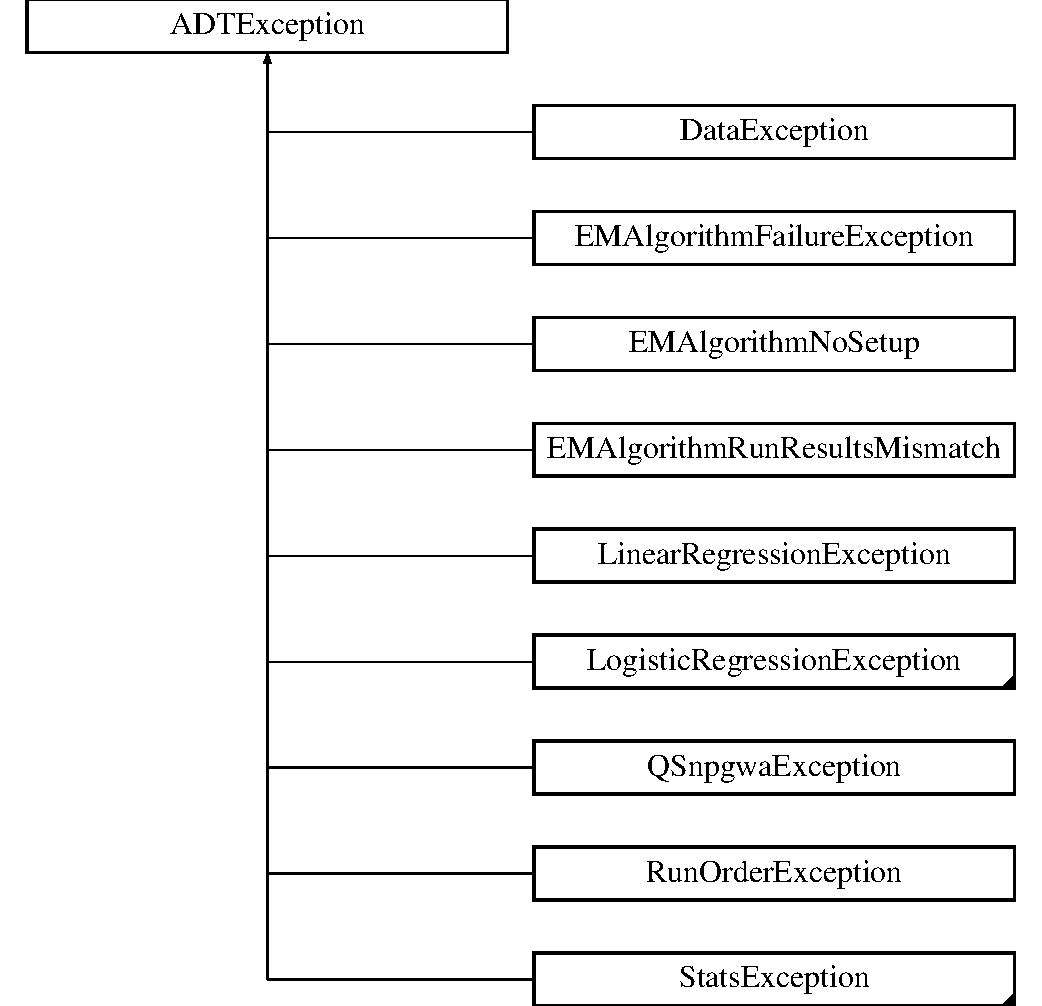
\includegraphics[height=10cm]{classADTException}
\end{center}
\end{figure}
\subsection*{Public Member Functions}
\begin{DoxyCompactItemize}
\item 
virtual \hyperlink{classADTException_ab46c90cf660ee52426bcd8db57205e54}{$\sim$ADTException} ()
\end{DoxyCompactItemize}


\subsection{Constructor \& Destructor Documentation}
\hypertarget{classADTException_ab46c90cf660ee52426bcd8db57205e54}{
\index{ADTException@{ADTException}!$\sim$ADTException@{$\sim$ADTException}}
\index{$\sim$ADTException@{$\sim$ADTException}!ADTException@{ADTException}}
\subsubsection[{$\sim$ADTException}]{\setlength{\rightskip}{0pt plus 5cm}virtual ADTException::$\sim$ADTException ()\hspace{0.3cm}{\ttfamily  \mbox{[}inline, virtual\mbox{]}}}}
\label{classADTException_ab46c90cf660ee52426bcd8db57205e54}


The documentation for this class was generated from the following file:\begin{DoxyCompactItemize}
\item 
engine/utils/\hyperlink{exceptions_8h}{exceptions.h}\end{DoxyCompactItemize}

\hypertarget{classADTree}{
\section{ADTree Class Reference}
\label{classADTree}\index{ADTree@{ADTree}}
}


{\ttfamily \#include $<$adtree.h$>$}

Inheritance diagram for ADTree:\begin{figure}[H]
\begin{center}
\leavevmode
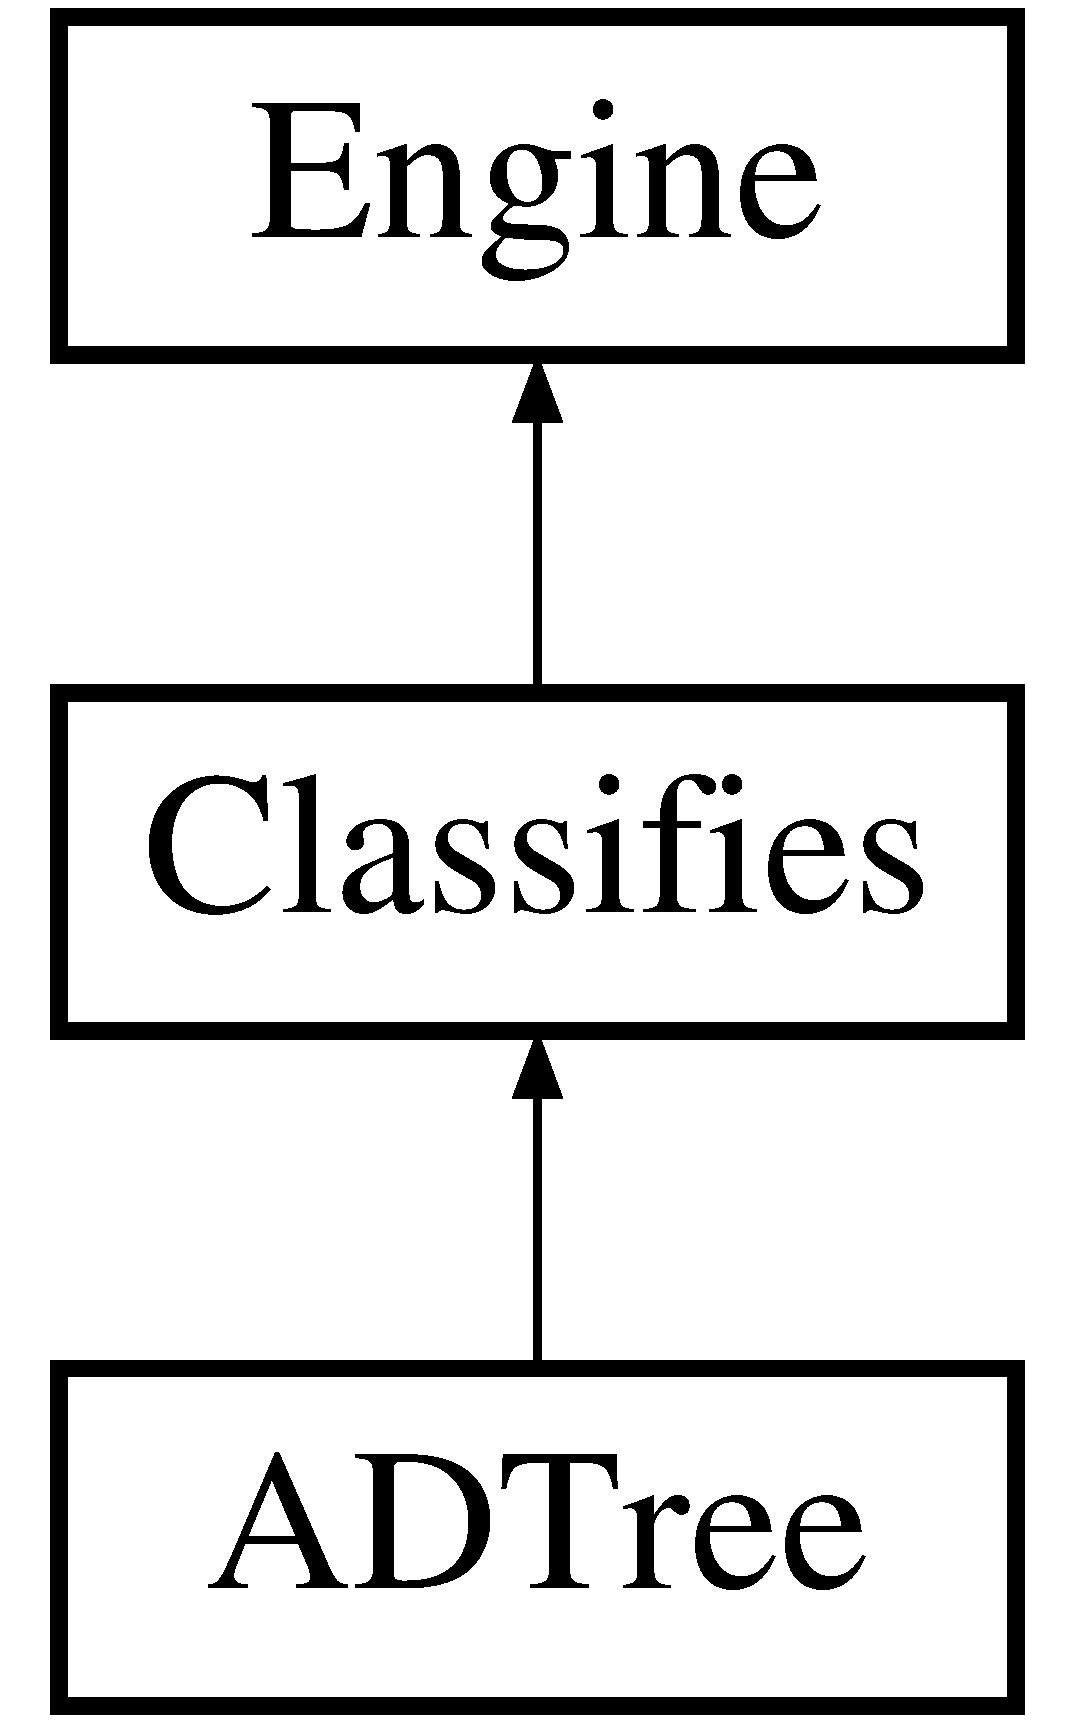
\includegraphics[height=3cm]{classADTree}
\end{center}
\end{figure}
\subsection*{Public Member Functions}
\begin{DoxyCompactItemize}
\item 
\hyperlink{classADTree_a4cc267cd53158a78c5812416b15477c6}{ADTree} ()
\item 
\hyperlink{classADTree_ae5069f6f5e8fc92a8fa8f687d0c6e911}{ADTree} (\hyperlink{classDataAccess}{DataAccess} $\ast$)
\item 
\hyperlink{classADTree_a42f89fabb90e742c8609af4618fc5fb7}{$\sim$ADTree} ()
\item 
virtual void \hyperlink{classADTree_a70b34e300c187fb817bc6d8ba31aceaa}{init} ()
\begin{DoxyCompactList}\small\item\em Must declare these as part of \hyperlink{classEngine}{Engine} abstract class. \item\end{DoxyCompactList}\item 
virtual void \hyperlink{classADTree_a18b7ad4befedb9073a83c39106628d3b}{preProcess} ()
\item 
virtual void \hyperlink{classADTree_acbdd5c7a248305933868e00bd875fd33}{process} ()
\item 
virtual void \hyperlink{classADTree_a4e89d611e7dc79fa8826efa742f9ce42}{enslave} (\hyperlink{classEngineParamReader}{EngineParamReader} $\ast$)
\item 
virtual void \hyperlink{classADTree_ac4183a7e36602b90e36e3717deef102c}{test} ()
\item 
void \hyperlink{classADTree_a544f723a8c49a74f554fb04d3a78cea6}{report} (map$<$ string, int $>$ \&, map$<$ string, \hyperlink{classAD__Rule}{AD\_\-Rule} $>$ \&)
\item 
void \hyperlink{classADTree_ab1fb3de26e2af354385c44eba2d17a98}{report\_\-leaves} (map$<$ string, int $>$ \&, map$<$ string, \hyperlink{classAD__Rule}{AD\_\-Rule} $>$ \&)
\item 
\hyperlink{classAD__Data}{AD\_\-Data} \hyperlink{classADTree_acd4ffcfe3f27fff312b143689b7add52}{get\_\-tree} ()
\item 
string \hyperlink{classADTree_a9b3d523c53bbfffe1988d72fb9791c87}{print\_\-tree} ()
\item 
void \hyperlink{classADTree_abb780d1ef5e6d66128dc990ce0189554}{print\_\-tree\_\-to\_\-file} ()
\item 
virtual void \hyperlink{classADTree_a335cdf83f845638ae6c74fa1d7e7e4b8}{classify} (int a\mbox{[}4\mbox{]})
\begin{DoxyCompactList}\small\item\em Classification. \item\end{DoxyCompactList}\item 
virtual void \hyperlink{classADTree_a498b7a7830dba60118e89d5f5bb7cbd3}{classify} (int a\mbox{[}4\mbox{]}, \hyperlink{classSnpData}{SnpData} $\ast$)
\item 
virtual int \hyperlink{classADTree_a266a816ec8750b5ceb1549ff610fb67b}{classify} (vector$<$ short $>$ \&)
\end{DoxyCompactItemize}
\subsection*{Protected Member Functions}
\begin{DoxyCompactItemize}
\item 
void \hyperlink{classADTree_a726e3f99718496cce2dbcf88c06e6b35}{weights} (double $\ast$, int, long, \hyperlink{classCondition_af41afbd9545b1fb2e2cb4a4792d52408}{Condition::comparison}, short)
\item 
void \hyperlink{classADTree_a75995e4c656f386c74450e7571b0dfcb}{weights2} (double $\ast$, int, long)
\item 
void \hyperlink{classADTree_a9026beb206f3f2f82c75e948876122da}{weights} (double $\ast$)
\item 
double \hyperlink{classADTree_a6e496b6bfad8f6b5db794728d7eaa426}{score\_\-categorical} (int, long, \hyperlink{classCondition_af41afbd9545b1fb2e2cb4a4792d52408}{Condition::comparison} \&, short \&)
\item 
double \hyperlink{classADTree_ab9b3c82b61aff738c450bd3b03a27631}{score\_\-ordinal} (int, long, short \&, vector$<$ double $>$ \&\hyperlink{classADTree_a3fdcc9137b95113198be7c4861516df0}{weight\_\-vec})
\item 
double \hyperlink{classADTree_a9afd1374b2b77b24cd766be6f4450db7}{minimize} (int $\ast$, long $\ast$, \hyperlink{classCondition_af41afbd9545b1fb2e2cb4a4792d52408}{Condition::comparison} $\ast$, short $\ast$)
\item 
double \hyperlink{classADTree_af44335915afb5cde9d3dcd59ab5de99c}{minimize\_\-ordinal} (int \&, long \&, \hyperlink{classCondition_af41afbd9545b1fb2e2cb4a4792d52408}{Condition::comparison} \&, short \&)
\item 
bool \hyperlink{classADTree_af693c7a7151e15c4c14af80a06fc971c}{keep\_\-going} ()
\item 
void \hyperlink{classADTree_ae6466f8f99be68c8f887b06c3d962964}{delete\_\-my\_\-innards} ()
\item 
void \hyperlink{classADTree_acd444c9e1e4fb4a95ee662f1be89c1cb}{processNoCov} ()
\end{DoxyCompactItemize}
\subsection*{Protected Attributes}
\begin{DoxyCompactItemize}
\item 
bool \hyperlink{classADTree_a7d81e0601304461d086b9bc134342a36}{haveOwner}
\item 
double \hyperlink{classADTree_a2e99a6dba3ab1a84e7323c8bd0990f02}{fudge}
\item 
vector$<$ double $>$ \hyperlink{classADTree_a3fdcc9137b95113198be7c4861516df0}{weight\_\-vec}
\item 
\hyperlink{classEngineParamReader}{EngineParamReader} $\ast$ \hyperlink{classADTree_a4640db912fa2d1f7c7798466d4a4bdc9}{ad\_\-param}
\item 
int \hyperlink{classADTree_ade70783ee662b06ea7e1030dbd25a978}{order\_\-in\_\-bag}
\item 
vector$<$ double $>$ \hyperlink{classADTree_a506c3976eb2bbfc129bdfe852886c801}{percentTrue}
\begin{DoxyCompactList}\small\item\em Used in stopping criteria. \item\end{DoxyCompactList}\item 
\hyperlink{classAD__Data}{AD\_\-Data} \hyperlink{classADTree_a8bfb36a2d5ded97c2d4ce61046996694}{tree}
\end{DoxyCompactItemize}


\subsection{Constructor \& Destructor Documentation}
\hypertarget{classADTree_a4cc267cd53158a78c5812416b15477c6}{
\index{ADTree@{ADTree}!ADTree@{ADTree}}
\index{ADTree@{ADTree}!ADTree@{ADTree}}
\subsubsection[{ADTree}]{\setlength{\rightskip}{0pt plus 5cm}ADTree::ADTree ()\hspace{0.3cm}{\ttfamily  \mbox{[}explicit\mbox{]}}}}
\label{classADTree_a4cc267cd53158a78c5812416b15477c6}
Set up the param\_\-reader, data classes. Leave the reader for init. \hypertarget{classADTree_ae5069f6f5e8fc92a8fa8f687d0c6e911}{
\index{ADTree@{ADTree}!ADTree@{ADTree}}
\index{ADTree@{ADTree}!ADTree@{ADTree}}
\subsubsection[{ADTree}]{\setlength{\rightskip}{0pt plus 5cm}ADTree::ADTree ({\bf DataAccess} $\ast$ {\em d})\hspace{0.3cm}{\ttfamily  \mbox{[}explicit\mbox{]}}}}
\label{classADTree_ae5069f6f5e8fc92a8fa8f687d0c6e911}
\hypertarget{classADTree_a42f89fabb90e742c8609af4618fc5fb7}{
\index{ADTree@{ADTree}!$\sim$ADTree@{$\sim$ADTree}}
\index{$\sim$ADTree@{$\sim$ADTree}!ADTree@{ADTree}}
\subsubsection[{$\sim$ADTree}]{\setlength{\rightskip}{0pt plus 5cm}ADTree::$\sim$ADTree ()}}
\label{classADTree_a42f89fabb90e742c8609af4618fc5fb7}


\subsection{Member Function Documentation}
\hypertarget{classADTree_a266a816ec8750b5ceb1549ff610fb67b}{
\index{ADTree@{ADTree}!classify@{classify}}
\index{classify@{classify}!ADTree@{ADTree}}
\subsubsection[{classify}]{\setlength{\rightskip}{0pt plus 5cm}int ADTree::classify (vector$<$ short $>$ \& {\em data})\hspace{0.3cm}{\ttfamily  \mbox{[}virtual\mbox{]}}}}
\label{classADTree_a266a816ec8750b5ceb1549ff610fb67b}
Return the classification for this individual. \begin{DoxyReturn}{Returns}
int 1 or -\/1 based on sign. 
\end{DoxyReturn}


Implements \hyperlink{classClassifies_a5e3d218b44024ec2c3ab3398e3dbd2e3}{Classifies}.

\hypertarget{classADTree_a498b7a7830dba60118e89d5f5bb7cbd3}{
\index{ADTree@{ADTree}!classify@{classify}}
\index{classify@{classify}!ADTree@{ADTree}}
\subsubsection[{classify}]{\setlength{\rightskip}{0pt plus 5cm}void ADTree::classify (int {\em a}\mbox{[}4\mbox{]}, \/  {\bf SnpData} $\ast$ {\em data})\hspace{0.3cm}{\ttfamily  \mbox{[}virtual\mbox{]}}}}
\label{classADTree_a498b7a7830dba60118e89d5f5bb7cbd3}


Implements \hyperlink{classClassifies_a7d2ae89f04af1a74eb6dd35be8eda476}{Classifies}.

\hypertarget{classADTree_a335cdf83f845638ae6c74fa1d7e7e4b8}{
\index{ADTree@{ADTree}!classify@{classify}}
\index{classify@{classify}!ADTree@{ADTree}}
\subsubsection[{classify}]{\setlength{\rightskip}{0pt plus 5cm}void ADTree::classify (int {\em a}\mbox{[}4\mbox{]})\hspace{0.3cm}{\ttfamily  \mbox{[}virtual\mbox{]}}}}
\label{classADTree_a335cdf83f845638ae6c74fa1d7e7e4b8}


Classification. 

name: \hyperlink{classADTree_a335cdf83f845638ae6c74fa1d7e7e4b8}{ADTree::classify} 
\begin{DoxyParams}{Parameters}
\item[{\em int}]a\mbox{[}4\mbox{]} will contain TP,FP,FN,TN counts for the individuals in this test set. Controls classified as controls would be in a\mbox{[}0\mbox{]} P and N are defined as $>$=, $<$ 0. \end{DoxyParams}


Implements \hyperlink{classClassifies_a15864d3a95edfde2bf48384c9b25c6d8}{Classifies}.

\hypertarget{classADTree_ae6466f8f99be68c8f887b06c3d962964}{
\index{ADTree@{ADTree}!delete\_\-my\_\-innards@{delete\_\-my\_\-innards}}
\index{delete\_\-my\_\-innards@{delete\_\-my\_\-innards}!ADTree@{ADTree}}
\subsubsection[{delete\_\-my\_\-innards}]{\setlength{\rightskip}{0pt plus 5cm}void ADTree::delete\_\-my\_\-innards ()\hspace{0.3cm}{\ttfamily  \mbox{[}protected\mbox{]}}}}
\label{classADTree_ae6466f8f99be68c8f887b06c3d962964}
\hypertarget{classADTree_a4e89d611e7dc79fa8826efa742f9ce42}{
\index{ADTree@{ADTree}!enslave@{enslave}}
\index{enslave@{enslave}!ADTree@{ADTree}}
\subsubsection[{enslave}]{\setlength{\rightskip}{0pt plus 5cm}void ADTree::enslave ({\bf EngineParamReader} $\ast$ {\em b})\hspace{0.3cm}{\ttfamily  \mbox{[}virtual\mbox{]}}}}
\label{classADTree_a4e89d611e7dc79fa8826efa742f9ce42}
Delete current adparam reader and replace it with the referant. 

Implements \hyperlink{classEngine_a023e094182312b1732fe53754c2fe5cb}{Engine}.

\hypertarget{classADTree_acd4ffcfe3f27fff312b143689b7add52}{
\index{ADTree@{ADTree}!get\_\-tree@{get\_\-tree}}
\index{get\_\-tree@{get\_\-tree}!ADTree@{ADTree}}
\subsubsection[{get\_\-tree}]{\setlength{\rightskip}{0pt plus 5cm}{\bf AD\_\-Data} ADTree::get\_\-tree ()\hspace{0.3cm}{\ttfamily  \mbox{[}inline\mbox{]}}}}
\label{classADTree_acd4ffcfe3f27fff312b143689b7add52}
\hypertarget{classADTree_a70b34e300c187fb817bc6d8ba31aceaa}{
\index{ADTree@{ADTree}!init@{init}}
\index{init@{init}!ADTree@{ADTree}}
\subsubsection[{init}]{\setlength{\rightskip}{0pt plus 5cm}void ADTree::init ()\hspace{0.3cm}{\ttfamily  \mbox{[}virtual\mbox{]}}}}
\label{classADTree_a70b34e300c187fb817bc6d8ba31aceaa}


Must declare these as part of \hyperlink{classEngine}{Engine} abstract class. 

\hyperlink{classADTree_a70b34e300c187fb817bc6d8ba31aceaa}{init()}

Set up the reader and input all data. Call the data checker in the snp\_\-data method. 

Implements \hyperlink{classEngine_aaa054d596fb8ced6e3eb4bee208f8c3d}{Engine}.

\hypertarget{classADTree_af693c7a7151e15c4c14af80a06fc971c}{
\index{ADTree@{ADTree}!keep\_\-going@{keep\_\-going}}
\index{keep\_\-going@{keep\_\-going}!ADTree@{ADTree}}
\subsubsection[{keep\_\-going}]{\setlength{\rightskip}{0pt plus 5cm}bool ADTree::keep\_\-going ()\hspace{0.3cm}{\ttfamily  \mbox{[}protected\mbox{]}}}}
\label{classADTree_af693c7a7151e15c4c14af80a06fc971c}
calculate stopping criteria for the main loop. The simplest scheme is to go based only on size. A more nuanced scheme will rely on sufficient decrease or (even better) on a mix of the two. \begin{DoxyReturn}{Returns}
boolean true if perform another round. 
\end{DoxyReturn}
\hypertarget{classADTree_a9afd1374b2b77b24cd766be6f4450db7}{
\index{ADTree@{ADTree}!minimize@{minimize}}
\index{minimize@{minimize}!ADTree@{ADTree}}
\subsubsection[{minimize}]{\setlength{\rightskip}{0pt plus 5cm}double ADTree::minimize (int $\ast$ {\em precon}, \/  long $\ast$ {\em attribute}, \/  {\bf Condition::comparison} $\ast$ {\em test}, \/  short $\ast$ {\em val})\hspace{0.3cm}{\ttfamily  \mbox{[}protected\mbox{]}}}}
\label{classADTree_a9afd1374b2b77b24cd766be6f4450db7}
Minimize the value Z(p,c) given in white paper.

Note: this will need to be done in parallel soon...

For each snp for each locus for each condition (roll this together) for each precondition get score and compare. \hypertarget{classADTree_af44335915afb5cde9d3dcd59ab5de99c}{
\index{ADTree@{ADTree}!minimize\_\-ordinal@{minimize\_\-ordinal}}
\index{minimize\_\-ordinal@{minimize\_\-ordinal}!ADTree@{ADTree}}
\subsubsection[{minimize\_\-ordinal}]{\setlength{\rightskip}{0pt plus 5cm}double ADTree::minimize\_\-ordinal (int \& {\em precon}, \/  long \& {\em attribute}, \/  {\bf Condition::comparison} \& {\em test}, \/  short \& {\em val})\hspace{0.3cm}{\ttfamily  \mbox{[}protected\mbox{]}}}}
\label{classADTree_af44335915afb5cde9d3dcd59ab5de99c}
Perform a minimization using each possible score from the set \{1,2,4\} \hypertarget{classADTree_a18b7ad4befedb9073a83c39106628d3b}{
\index{ADTree@{ADTree}!preProcess@{preProcess}}
\index{preProcess@{preProcess}!ADTree@{ADTree}}
\subsubsection[{preProcess}]{\setlength{\rightskip}{0pt plus 5cm}void ADTree::preProcess ()\hspace{0.3cm}{\ttfamily  \mbox{[}virtual\mbox{]}}}}
\label{classADTree_a18b7ad4befedb9073a83c39106628d3b}
\hyperlink{classADTree_a18b7ad4befedb9073a83c39106628d3b}{preProcess()}

Push the head node onto the stack. 

Implements \hyperlink{classEngine_aec7076b8979a13c96eceb362437dc68c}{Engine}.

\hypertarget{classADTree_a9b3d523c53bbfffe1988d72fb9791c87}{
\index{ADTree@{ADTree}!print\_\-tree@{print\_\-tree}}
\index{print\_\-tree@{print\_\-tree}!ADTree@{ADTree}}
\subsubsection[{print\_\-tree}]{\setlength{\rightskip}{0pt plus 5cm}string ADTree::print\_\-tree ()\hspace{0.3cm}{\ttfamily  \mbox{[}inline\mbox{]}}}}
\label{classADTree_a9b3d523c53bbfffe1988d72fb9791c87}
\hypertarget{classADTree_abb780d1ef5e6d66128dc990ce0189554}{
\index{ADTree@{ADTree}!print\_\-tree\_\-to\_\-file@{print\_\-tree\_\-to\_\-file}}
\index{print\_\-tree\_\-to\_\-file@{print\_\-tree\_\-to\_\-file}!ADTree@{ADTree}}
\subsubsection[{print\_\-tree\_\-to\_\-file}]{\setlength{\rightskip}{0pt plus 5cm}void ADTree::print\_\-tree\_\-to\_\-file ()}}
\label{classADTree_abb780d1ef5e6d66128dc990ce0189554}
Print the tree to a file. \hypertarget{classADTree_acbdd5c7a248305933868e00bd875fd33}{
\index{ADTree@{ADTree}!process@{process}}
\index{process@{process}!ADTree@{ADTree}}
\subsubsection[{process}]{\setlength{\rightskip}{0pt plus 5cm}void ADTree::process ()\hspace{0.3cm}{\ttfamily  \mbox{[}virtual\mbox{]}}}}
\label{classADTree_acbdd5c7a248305933868e00bd875fd33}
\hyperlink{classADTree_acbdd5c7a248305933868e00bd875fd33}{process()}

This calls the guts. Start the algorithm and run it.

If there are covariates, run them first. 

Implements \hyperlink{classEngine_a005f8e277c3dea16ea05803fba223db7}{Engine}.

\hypertarget{classADTree_acd444c9e1e4fb4a95ee662f1be89c1cb}{
\index{ADTree@{ADTree}!processNoCov@{processNoCov}}
\index{processNoCov@{processNoCov}!ADTree@{ADTree}}
\subsubsection[{processNoCov}]{\setlength{\rightskip}{0pt plus 5cm}void ADTree::processNoCov ()\hspace{0.3cm}{\ttfamily  \mbox{[}protected\mbox{]}}}}
\label{classADTree_acd444c9e1e4fb4a95ee662f1be89c1cb}
Build the \hyperlink{classADTree}{ADTree}, assuming no covariates. \hypertarget{classADTree_a544f723a8c49a74f554fb04d3a78cea6}{
\index{ADTree@{ADTree}!report@{report}}
\index{report@{report}!ADTree@{ADTree}}
\subsubsection[{report}]{\setlength{\rightskip}{0pt plus 5cm}void ADTree::report (map$<$ string, int $>$ \& {\em hash}, \/  map$<$ string, {\bf AD\_\-Rule} $>$ \& {\em key})}}
\label{classADTree_a544f723a8c49a74f554fb04d3a78cea6}
\hypertarget{classADTree_ab1fb3de26e2af354385c44eba2d17a98}{
\index{ADTree@{ADTree}!report\_\-leaves@{report\_\-leaves}}
\index{report\_\-leaves@{report\_\-leaves}!ADTree@{ADTree}}
\subsubsection[{report\_\-leaves}]{\setlength{\rightskip}{0pt plus 5cm}void ADTree::report\_\-leaves (map$<$ string, int $>$ \& {\em hash}, \/  map$<$ string, {\bf AD\_\-Rule} $>$ \& {\em key})}}
\label{classADTree_ab1fb3de26e2af354385c44eba2d17a98}
\hypertarget{classADTree_a6e496b6bfad8f6b5db794728d7eaa426}{
\index{ADTree@{ADTree}!score\_\-categorical@{score\_\-categorical}}
\index{score\_\-categorical@{score\_\-categorical}!ADTree@{ADTree}}
\subsubsection[{score\_\-categorical}]{\setlength{\rightskip}{0pt plus 5cm}double ADTree::score\_\-categorical (int {\em r}, \/  long {\em i}, \/  {\bf Condition::comparison} \& {\em c}, \/  short \& {\em s})\hspace{0.3cm}{\ttfamily  \mbox{[}protected\mbox{]}}}}
\label{classADTree_a6e496b6bfad8f6b5db794728d7eaa426}
score\_\-categorical

Perform scoring for a given precondition and variable.


\begin{DoxyParams}{Parameters}
\item[{\em int}]r: \hyperlink{classPrecondition}{Precondition} in use \item[{\em long}]i: SNP in use \item[{\em \hyperlink{classCondition_af41afbd9545b1fb2e2cb4a4792d52408}{Condition::comparison}}]\&: Type of comparison returned. \item[{\em short}]s: Optimal split point. \end{DoxyParams}
\hypertarget{classADTree_ab9b3c82b61aff738c450bd3b03a27631}{
\index{ADTree@{ADTree}!score\_\-ordinal@{score\_\-ordinal}}
\index{score\_\-ordinal@{score\_\-ordinal}!ADTree@{ADTree}}
\subsubsection[{score\_\-ordinal}]{\setlength{\rightskip}{0pt plus 5cm}double ADTree::score\_\-ordinal (int {\em pre\_\-cond}, \/  long {\em snp}, \/  short \& {\em s}, \/  vector$<$ double $>$ \& {\em temp\_\-weights})\hspace{0.3cm}{\ttfamily  \mbox{[}protected\mbox{]}}}}
\label{classADTree_ab9b3c82b61aff738c450bd3b03a27631}
Score for ordinal, which treats each type separately.

This is a customized version of the minimization in ADTrees that was created by Richard T. Guy and is under current investigation. \hypertarget{classADTree_ac4183a7e36602b90e36e3717deef102c}{
\index{ADTree@{ADTree}!test@{test}}
\index{test@{test}!ADTree@{ADTree}}
\subsubsection[{test}]{\setlength{\rightskip}{0pt plus 5cm}void ADTree::test ()\hspace{0.3cm}{\ttfamily  \mbox{[}virtual\mbox{]}}}}
\label{classADTree_ac4183a7e36602b90e36e3717deef102c}
Perform a few tests, see internal comments. 

Implements \hyperlink{classEngine_a2927c4a4263809453063ad482c6434a4}{Engine}.

\hypertarget{classADTree_a9026beb206f3f2f82c75e948876122da}{
\index{ADTree@{ADTree}!weights@{weights}}
\index{weights@{weights}!ADTree@{ADTree}}
\subsubsection[{weights}]{\setlength{\rightskip}{0pt plus 5cm}void ADTree::weights (double $\ast$ {\em ret\_\-weight})\hspace{0.3cm}{\ttfamily  \mbox{[}protected\mbox{]}}}}
\label{classADTree_a9026beb206f3f2f82c75e948876122da}
Simply calculate weights for pos or neg class (1 or 2 in my coding) Completely skip missings.

Returns \mbox{[}phen==2,phen==1\mbox{]} for W\_\-+, W\_\--\/ \hypertarget{classADTree_a726e3f99718496cce2dbcf88c06e6b35}{
\index{ADTree@{ADTree}!weights@{weights}}
\index{weights@{weights}!ADTree@{ADTree}}
\subsubsection[{weights}]{\setlength{\rightskip}{0pt plus 5cm}void ADTree::weights (double $\ast$ {\em ret\_\-weights}, \/  int {\em pre\_\-cond}, \/  long {\em attribute}, \/  {\bf Condition::comparison} {\em test}, \/  short {\em val})\hspace{0.3cm}{\ttfamily  \mbox{[}protected\mbox{]}}}}
\label{classADTree_a726e3f99718496cce2dbcf88c06e6b35}
This is more extensible, but if data is known, use weights2 for speed. Calc total weights of all individuals that satisfy each of the conditions.

W\_\-2 means are a 2 in phenotype.

Passed the weight vector, as well as an index to the rule under the precondition, the attribute to test against test type (see \hyperlink{condition_8h}{condition.h}) and the value we are comparing to. This could also be a \hyperlink{classCondition}{Condition} object but I don't want to build one every time we use this method (waste of cycles...)

Returned in ret\_\-weights: 0 -\/$>$ W\_\-1 for p and c (W\_\-+(p and c)) where W\_\-+ is phenotype 1. 1 -\/$>$ W\_\-2 for p and c (W\_\--\/(p and c)) 2 -\/$>$ W\_\-1 for p and not c (W\_\-+(p and c)) 3 -\/$>$ W\_\-2 for p and not c 4 -\/$>$ W\_\-1 or W\_\-2 and not p

A better strategy would be to return the count for each value of the categorical variable. \hypertarget{classADTree_a75995e4c656f386c74450e7571b0dfcb}{
\index{ADTree@{ADTree}!weights2@{weights2}}
\index{weights2@{weights2}!ADTree@{ADTree}}
\subsubsection[{weights2}]{\setlength{\rightskip}{0pt plus 5cm}void ADTree::weights2 (double $\ast$ {\em ret\_\-weights}, \/  int {\em pre\_\-cond}, \/  long {\em attribute})\hspace{0.3cm}{\ttfamily  \mbox{[}protected\mbox{]}}}}
\label{classADTree_a75995e4c656f386c74450e7571b0dfcb}
Calc W\_\-+ and W\_\--\/ for each possible value of genotype and each value of p \&\& c, p \&\& !c. Also, calculate for !p, which does not differentiate phenotypes.


\begin{DoxyParams}{Parameters}
\item[{\em Vector}]of weights to be filled. \item[{\em long}]attribute on which we fill. \end{DoxyParams}


\subsection{Field Documentation}
\hypertarget{classADTree_a4640db912fa2d1f7c7798466d4a4bdc9}{
\index{ADTree@{ADTree}!ad\_\-param@{ad\_\-param}}
\index{ad\_\-param@{ad\_\-param}!ADTree@{ADTree}}
\subsubsection[{ad\_\-param}]{\setlength{\rightskip}{0pt plus 5cm}{\bf EngineParamReader}$\ast$ {\bf ADTree::ad\_\-param}\hspace{0.3cm}{\ttfamily  \mbox{[}protected\mbox{]}}}}
\label{classADTree_a4640db912fa2d1f7c7798466d4a4bdc9}
\hypertarget{classADTree_a2e99a6dba3ab1a84e7323c8bd0990f02}{
\index{ADTree@{ADTree}!fudge@{fudge}}
\index{fudge@{fudge}!ADTree@{ADTree}}
\subsubsection[{fudge}]{\setlength{\rightskip}{0pt plus 5cm}double {\bf ADTree::fudge}\hspace{0.3cm}{\ttfamily  \mbox{[}protected\mbox{]}}}}
\label{classADTree_a2e99a6dba3ab1a84e7323c8bd0990f02}
\hypertarget{classADTree_a7d81e0601304461d086b9bc134342a36}{
\index{ADTree@{ADTree}!haveOwner@{haveOwner}}
\index{haveOwner@{haveOwner}!ADTree@{ADTree}}
\subsubsection[{haveOwner}]{\setlength{\rightskip}{0pt plus 5cm}bool {\bf ADTree::haveOwner}\hspace{0.3cm}{\ttfamily  \mbox{[}protected\mbox{]}}}}
\label{classADTree_a7d81e0601304461d086b9bc134342a36}
\hypertarget{classADTree_ade70783ee662b06ea7e1030dbd25a978}{
\index{ADTree@{ADTree}!order\_\-in\_\-bag@{order\_\-in\_\-bag}}
\index{order\_\-in\_\-bag@{order\_\-in\_\-bag}!ADTree@{ADTree}}
\subsubsection[{order\_\-in\_\-bag}]{\setlength{\rightskip}{0pt plus 5cm}int {\bf ADTree::order\_\-in\_\-bag}\hspace{0.3cm}{\ttfamily  \mbox{[}protected\mbox{]}}}}
\label{classADTree_ade70783ee662b06ea7e1030dbd25a978}
\hypertarget{classADTree_a506c3976eb2bbfc129bdfe852886c801}{
\index{ADTree@{ADTree}!percentTrue@{percentTrue}}
\index{percentTrue@{percentTrue}!ADTree@{ADTree}}
\subsubsection[{percentTrue}]{\setlength{\rightskip}{0pt plus 5cm}vector$<$double$>$ {\bf ADTree::percentTrue}\hspace{0.3cm}{\ttfamily  \mbox{[}protected\mbox{]}}}}
\label{classADTree_a506c3976eb2bbfc129bdfe852886c801}


Used in stopping criteria. 

\hypertarget{classADTree_a8bfb36a2d5ded97c2d4ce61046996694}{
\index{ADTree@{ADTree}!tree@{tree}}
\index{tree@{tree}!ADTree@{ADTree}}
\subsubsection[{tree}]{\setlength{\rightskip}{0pt plus 5cm}{\bf AD\_\-Data} {\bf ADTree::tree}\hspace{0.3cm}{\ttfamily  \mbox{[}protected\mbox{]}}}}
\label{classADTree_a8bfb36a2d5ded97c2d4ce61046996694}
\hypertarget{classADTree_a3fdcc9137b95113198be7c4861516df0}{
\index{ADTree@{ADTree}!weight\_\-vec@{weight\_\-vec}}
\index{weight\_\-vec@{weight\_\-vec}!ADTree@{ADTree}}
\subsubsection[{weight\_\-vec}]{\setlength{\rightskip}{0pt plus 5cm}vector$<$double$>$ {\bf ADTree::weight\_\-vec}\hspace{0.3cm}{\ttfamily  \mbox{[}protected\mbox{]}}}}
\label{classADTree_a3fdcc9137b95113198be7c4861516df0}


The documentation for this class was generated from the following files:\begin{DoxyCompactItemize}
\item 
engine/adtree/\hyperlink{adtree_8h}{adtree.h}\item 
engine/adtree/\hyperlink{adtree_8cpp}{adtree.cpp}\end{DoxyCompactItemize}

\hypertarget{classhaplotype_1_1alleleNumOutsideRangeEx}{
\section{haplotype::alleleNumOutsideRangeEx Class Reference}
\label{classhaplotype_1_1alleleNumOutsideRangeEx}\index{haplotype::alleleNumOutsideRangeEx@{haplotype::alleleNumOutsideRangeEx}}
}


{\ttfamily \#include $<$haplotype.h$>$}



The documentation for this class was generated from the following file:\begin{DoxyCompactItemize}
\item 
engine/em/\hyperlink{haplotype_8h}{haplotype.h}\end{DoxyCompactItemize}

\hypertarget{classArffReader}{
\section{ArffReader Class Reference}
\label{classArffReader}\index{ArffReader@{ArffReader}}
}


{\ttfamily \#include $<$arff\_\-reader.h$>$}

Inheritance diagram for ArffReader:\begin{figure}[H]
\begin{center}
\leavevmode
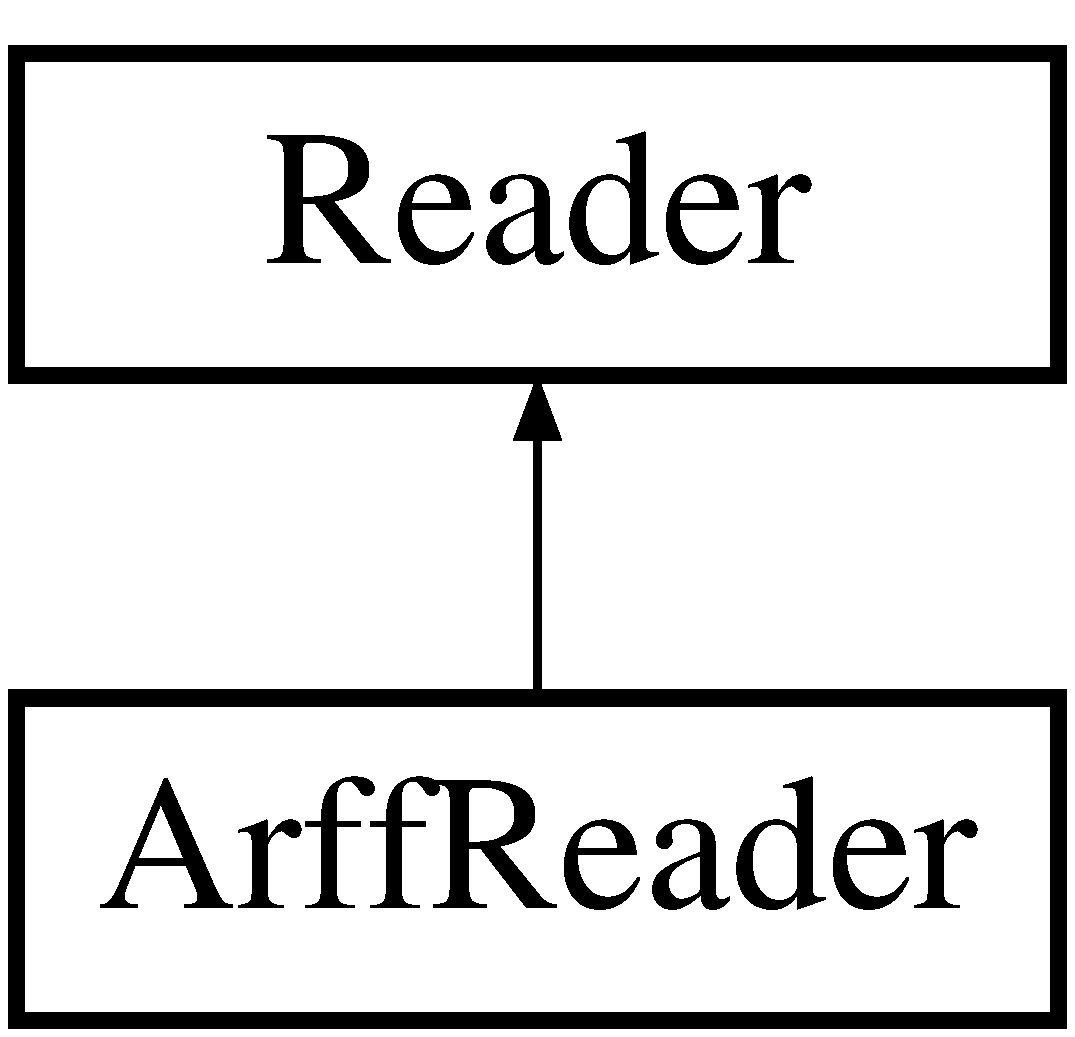
\includegraphics[height=2cm]{classArffReader}
\end{center}
\end{figure}
\subsection*{Public Member Functions}
\begin{DoxyCompactItemize}
\item 
\hyperlink{classArffReader_a2981a55a94b575b0370a14d0991ffb05}{ArffReader} ()
\item 
virtual void \hyperlink{classArffReader_af12ed42f6e726a6e336f22381ca84082}{process} (\hyperlink{classSnpData}{SnpData} $\ast$, \hyperlink{classParamReader}{ParamReader} $\ast$)
\end{DoxyCompactItemize}


\subsection{Constructor \& Destructor Documentation}
\hypertarget{classArffReader_a2981a55a94b575b0370a14d0991ffb05}{
\index{ArffReader@{ArffReader}!ArffReader@{ArffReader}}
\index{ArffReader@{ArffReader}!ArffReader@{ArffReader}}
\subsubsection[{ArffReader}]{\setlength{\rightskip}{0pt plus 5cm}ArffReader::ArffReader ()}}
\label{classArffReader_a2981a55a94b575b0370a14d0991ffb05}


\subsection{Member Function Documentation}
\hypertarget{classArffReader_af12ed42f6e726a6e336f22381ca84082}{
\index{ArffReader@{ArffReader}!process@{process}}
\index{process@{process}!ArffReader@{ArffReader}}
\subsubsection[{process}]{\setlength{\rightskip}{0pt plus 5cm}void ArffReader::process ({\bf SnpData} $\ast$ {\em data}, \/  {\bf ParamReader} $\ast$ {\em params})\hspace{0.3cm}{\ttfamily  \mbox{[}virtual\mbox{]}}}}
\label{classArffReader_af12ed42f6e726a6e336f22381ca84082}
Process the arff file, placing it in snp data. The parameter reader passed in will contain the location of the file, ect. 

Implements \hyperlink{classReader_a334a724f607c84262af67759ffcdbd26}{Reader}.



The documentation for this class was generated from the following files:\begin{DoxyCompactItemize}
\item 
reader/\hyperlink{arff__reader_8h}{arff\_\-reader.h}\item 
reader/\hyperlink{arff__reader_8cpp}{arff\_\-reader.cpp}\end{DoxyCompactItemize}

\hypertarget{classBagging}{
\section{Bagging Class Reference}
\label{classBagging}\index{Bagging@{Bagging}}
}


{\ttfamily \#include $<$bagging.h$>$}

Inheritance diagram for Bagging:\begin{figure}[H]
\begin{center}
\leavevmode
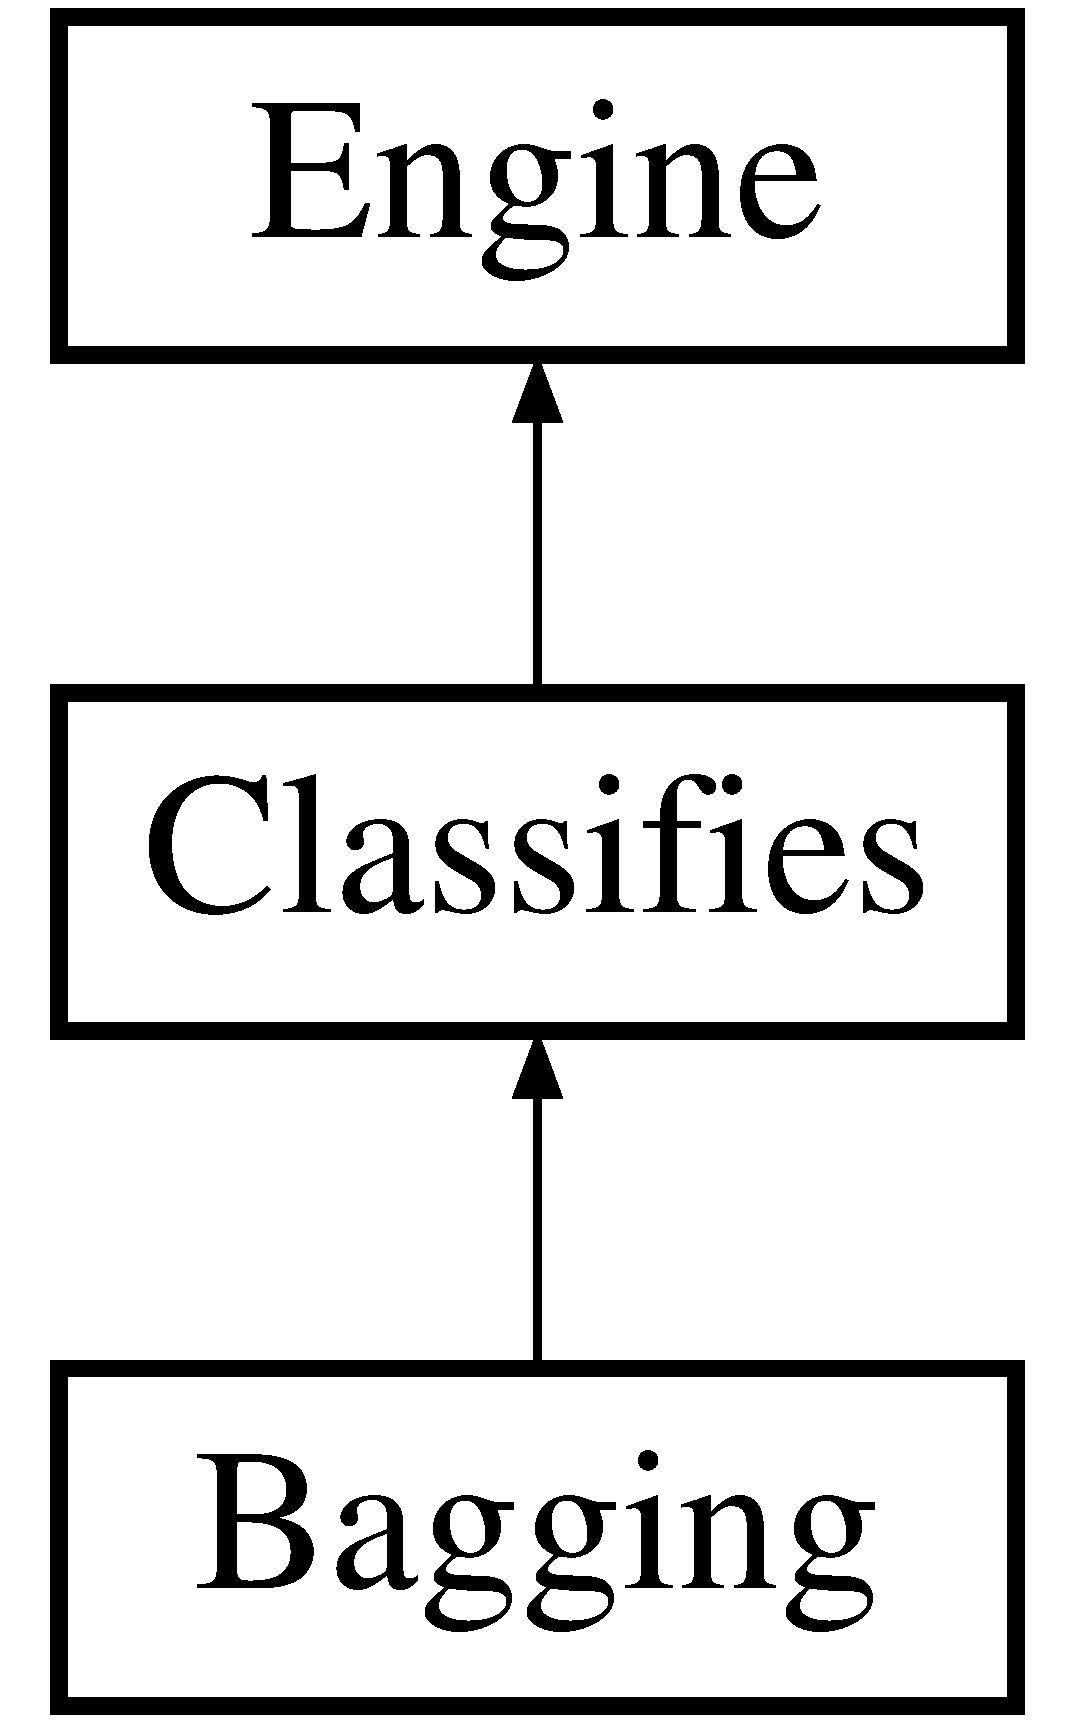
\includegraphics[height=3cm]{classBagging}
\end{center}
\end{figure}
\subsection*{Public Member Functions}
\begin{DoxyCompactItemize}
\item 
\hyperlink{classBagging_a3af2b221856ad4c4d4e2ef06441fcc84}{Bagging} ()
\item 
\hyperlink{classBagging_a144056cea8677b2365c3c15e87f5d38c}{Bagging} (\hyperlink{classDataAccess}{DataAccess} $\ast$)
\item 
virtual \hyperlink{classBagging_a25ed2b1fad2c85b4d3e562d7a332d369}{$\sim$Bagging} ()
\item 
virtual void \hyperlink{classBagging_ab58c678f776356ae4b4c1c41dcdf3778}{init} ()
\begin{DoxyCompactList}\small\item\em From Engine.h. \item\end{DoxyCompactList}\item 
virtual void \hyperlink{classBagging_a638e97695ee9a685cfee7ce459c2b8f8}{preProcess} ()
\item 
virtual void \hyperlink{classBagging_ab732c0768147c13071d4fc23d879dfd4}{process} ()
\item 
virtual void \hyperlink{classBagging_aa1f58fca264385a46fa7c14a5620488c}{enslave} (\hyperlink{classEngineParamReader}{EngineParamReader} $\ast$)
\item 
virtual void \hyperlink{classBagging_afd3022e8be01cba7f97fc9f81cda8016}{test} ()
\item 
virtual void \hyperlink{classBagging_a02227120bc610a21f39f2454ac03ec7b}{classify} (int a\mbox{[}4\mbox{]})
\begin{DoxyCompactList}\small\item\em Classification. \item\end{DoxyCompactList}\item 
virtual void \hyperlink{classBagging_a9b17e15983996f8ae3b39564e7c3deba}{classify} (int a\mbox{[}4\mbox{]}, \hyperlink{classSnpData}{SnpData} $\ast$)
\item 
virtual int \hyperlink{classBagging_a92072d6610e9b9d932d10a123cc6ff18}{classify} (vector$<$ short $>$ \&)
\end{DoxyCompactItemize}


\subsection{Detailed Description}
\hyperlink{classBagging}{Bagging} wrapper. Utilizes another engine to analyze bootstrap samples.

Author: Richard T. Guy 

\subsection{Constructor \& Destructor Documentation}
\hypertarget{classBagging_a3af2b221856ad4c4d4e2ef06441fcc84}{
\index{Bagging@{Bagging}!Bagging@{Bagging}}
\index{Bagging@{Bagging}!Bagging@{Bagging}}
\subsubsection[{Bagging}]{\setlength{\rightskip}{0pt plus 5cm}Bagging::Bagging ()\hspace{0.3cm}{\ttfamily  \mbox{[}explicit\mbox{]}}}}
\label{classBagging_a3af2b221856ad4c4d4e2ef06441fcc84}
\hypertarget{classBagging_a144056cea8677b2365c3c15e87f5d38c}{
\index{Bagging@{Bagging}!Bagging@{Bagging}}
\index{Bagging@{Bagging}!Bagging@{Bagging}}
\subsubsection[{Bagging}]{\setlength{\rightskip}{0pt plus 5cm}Bagging::Bagging ({\bf DataAccess} $\ast$ {\em d})\hspace{0.3cm}{\ttfamily  \mbox{[}explicit\mbox{]}}}}
\label{classBagging_a144056cea8677b2365c3c15e87f5d38c}
\hypertarget{classBagging_a25ed2b1fad2c85b4d3e562d7a332d369}{
\index{Bagging@{Bagging}!$\sim$Bagging@{$\sim$Bagging}}
\index{$\sim$Bagging@{$\sim$Bagging}!Bagging@{Bagging}}
\subsubsection[{$\sim$Bagging}]{\setlength{\rightskip}{0pt plus 5cm}Bagging::$\sim$Bagging ()\hspace{0.3cm}{\ttfamily  \mbox{[}virtual\mbox{]}}}}
\label{classBagging_a25ed2b1fad2c85b4d3e562d7a332d369}


\subsection{Member Function Documentation}
\hypertarget{classBagging_a92072d6610e9b9d932d10a123cc6ff18}{
\index{Bagging@{Bagging}!classify@{classify}}
\index{classify@{classify}!Bagging@{Bagging}}
\subsubsection[{classify}]{\setlength{\rightskip}{0pt plus 5cm}int Bagging::classify (vector$<$ short $>$ \&)\hspace{0.3cm}{\ttfamily  \mbox{[}virtual\mbox{]}}}}
\label{classBagging_a92072d6610e9b9d932d10a123cc6ff18}


Implements \hyperlink{classClassifies_a5e3d218b44024ec2c3ab3398e3dbd2e3}{Classifies}.

\hypertarget{classBagging_a9b17e15983996f8ae3b39564e7c3deba}{
\index{Bagging@{Bagging}!classify@{classify}}
\index{classify@{classify}!Bagging@{Bagging}}
\subsubsection[{classify}]{\setlength{\rightskip}{0pt plus 5cm}void Bagging::classify (int {\em a}\mbox{[}4\mbox{]}, \/  {\bf SnpData} $\ast$)\hspace{0.3cm}{\ttfamily  \mbox{[}virtual\mbox{]}}}}
\label{classBagging_a9b17e15983996f8ae3b39564e7c3deba}


Implements \hyperlink{classClassifies_a7d2ae89f04af1a74eb6dd35be8eda476}{Classifies}.

\hypertarget{classBagging_a02227120bc610a21f39f2454ac03ec7b}{
\index{Bagging@{Bagging}!classify@{classify}}
\index{classify@{classify}!Bagging@{Bagging}}
\subsubsection[{classify}]{\setlength{\rightskip}{0pt plus 5cm}void Bagging::classify (int {\em a}\mbox{[}4\mbox{]})\hspace{0.3cm}{\ttfamily  \mbox{[}virtual\mbox{]}}}}
\label{classBagging_a02227120bc610a21f39f2454ac03ec7b}


Classification. 



Implements \hyperlink{classClassifies_a15864d3a95edfde2bf48384c9b25c6d8}{Classifies}.

\hypertarget{classBagging_aa1f58fca264385a46fa7c14a5620488c}{
\index{Bagging@{Bagging}!enslave@{enslave}}
\index{enslave@{enslave}!Bagging@{Bagging}}
\subsubsection[{enslave}]{\setlength{\rightskip}{0pt plus 5cm}void Bagging::enslave ({\bf EngineParamReader} $\ast$ {\em b})\hspace{0.3cm}{\ttfamily  \mbox{[}virtual\mbox{]}}}}
\label{classBagging_aa1f58fca264385a46fa7c14a5620488c}
Delete current adparam reader and replace it with the referant. 

Implements \hyperlink{classEngine_a023e094182312b1732fe53754c2fe5cb}{Engine}.

\hypertarget{classBagging_ab58c678f776356ae4b4c1c41dcdf3778}{
\index{Bagging@{Bagging}!init@{init}}
\index{init@{init}!Bagging@{Bagging}}
\subsubsection[{init}]{\setlength{\rightskip}{0pt plus 5cm}void Bagging::init ()\hspace{0.3cm}{\ttfamily  \mbox{[}virtual\mbox{]}}}}
\label{classBagging_ab58c678f776356ae4b4c1c41dcdf3778}


From Engine.h. 

Retrieve data from files, prep data.

Only called if this is not a slave. 

Implements \hyperlink{classEngine_aaa054d596fb8ced6e3eb4bee208f8c3d}{Engine}.

\hypertarget{classBagging_a638e97695ee9a685cfee7ce459c2b8f8}{
\index{Bagging@{Bagging}!preProcess@{preProcess}}
\index{preProcess@{preProcess}!Bagging@{Bagging}}
\subsubsection[{preProcess}]{\setlength{\rightskip}{0pt plus 5cm}void Bagging::preProcess ()\hspace{0.3cm}{\ttfamily  \mbox{[}virtual\mbox{]}}}}
\label{classBagging_a638e97695ee9a685cfee7ce459c2b8f8}
Create bootstrap samples for every set by calling the snp\_\-data set. Right now we are always using the same size. 

Implements \hyperlink{classEngine_aec7076b8979a13c96eceb362437dc68c}{Engine}.

\hypertarget{classBagging_ab732c0768147c13071d4fc23d879dfd4}{
\index{Bagging@{Bagging}!process@{process}}
\index{process@{process}!Bagging@{Bagging}}
\subsubsection[{process}]{\setlength{\rightskip}{0pt plus 5cm}void Bagging::process ()\hspace{0.3cm}{\ttfamily  \mbox{[}virtual\mbox{]}}}}
\label{classBagging_ab732c0768147c13071d4fc23d879dfd4}


Implements \hyperlink{classEngine_a005f8e277c3dea16ea05803fba223db7}{Engine}.

\hypertarget{classBagging_afd3022e8be01cba7f97fc9f81cda8016}{
\index{Bagging@{Bagging}!test@{test}}
\index{test@{test}!Bagging@{Bagging}}
\subsubsection[{test}]{\setlength{\rightskip}{0pt plus 5cm}void Bagging::test ()\hspace{0.3cm}{\ttfamily  \mbox{[}virtual\mbox{]}}}}
\label{classBagging_afd3022e8be01cba7f97fc9f81cda8016}


Implements \hyperlink{classEngine_a2927c4a4263809453063ad482c6434a4}{Engine}.



The documentation for this class was generated from the following files:\begin{DoxyCompactItemize}
\item 
engine/bagging/\hyperlink{bagging_8h}{bagging.h}\item 
engine/bagging/\hyperlink{bagging_8cpp}{bagging.cpp}\end{DoxyCompactItemize}

\hypertarget{classBinaryBedReader}{
\section{BinaryBedReader Class Reference}
\label{classBinaryBedReader}\index{BinaryBedReader@{BinaryBedReader}}
}


{\ttfamily \#include $<$binary\_\-bed\_\-reader.h$>$}

Inheritance diagram for BinaryBedReader:\begin{figure}[H]
\begin{center}
\leavevmode
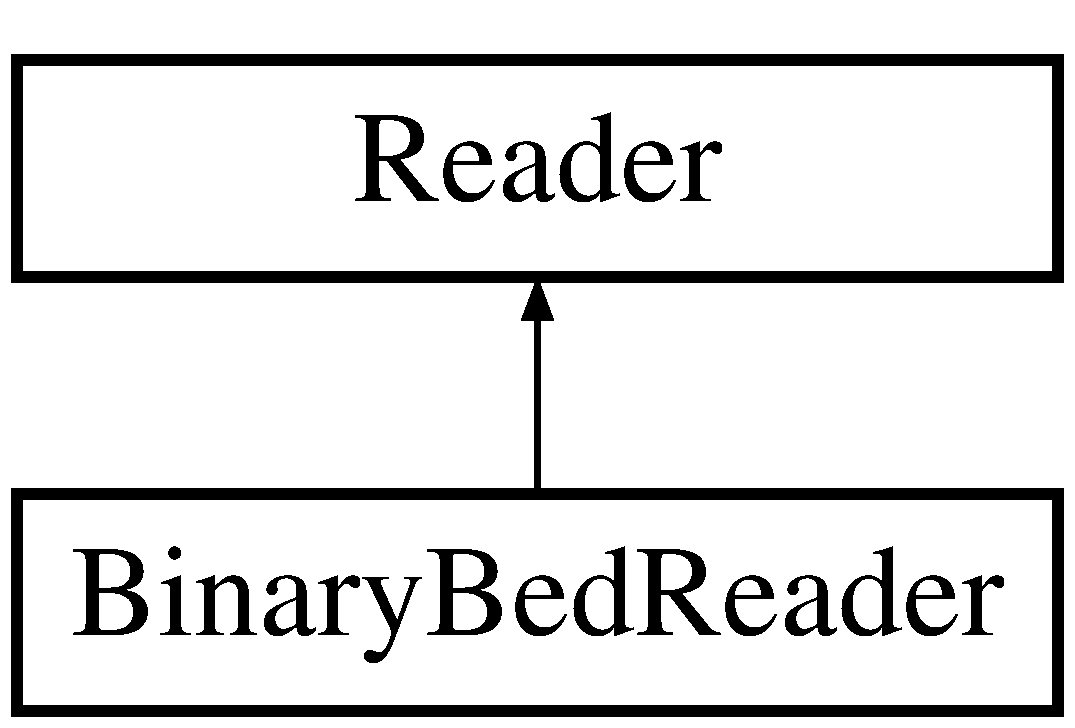
\includegraphics[height=2cm]{classBinaryBedReader}
\end{center}
\end{figure}
\subsection*{Public Member Functions}
\begin{DoxyCompactItemize}
\item 
\hyperlink{classBinaryBedReader_a34d61ea79646fbaf3d62c3c1c14b106e}{BinaryBedReader} ()
\item 
\hyperlink{classBinaryBedReader_aec2a611238224f6a436c080dec743c38}{$\sim$BinaryBedReader} ()
\item 
virtual void \hyperlink{classBinaryBedReader_a2132af8b71a683550c19ec4ac3ec3db2}{process} (\hyperlink{classSnpData}{SnpData} $\ast$, \hyperlink{classParamReader}{ParamReader} $\ast$)
\end{DoxyCompactItemize}


\subsection{Constructor \& Destructor Documentation}
\hypertarget{classBinaryBedReader_a34d61ea79646fbaf3d62c3c1c14b106e}{
\index{BinaryBedReader@{BinaryBedReader}!BinaryBedReader@{BinaryBedReader}}
\index{BinaryBedReader@{BinaryBedReader}!BinaryBedReader@{BinaryBedReader}}
\subsubsection[{BinaryBedReader}]{\setlength{\rightskip}{0pt plus 5cm}BinaryBedReader::BinaryBedReader ()}}
\label{classBinaryBedReader_a34d61ea79646fbaf3d62c3c1c14b106e}
\hypertarget{classBinaryBedReader_aec2a611238224f6a436c080dec743c38}{
\index{BinaryBedReader@{BinaryBedReader}!$\sim$BinaryBedReader@{$\sim$BinaryBedReader}}
\index{$\sim$BinaryBedReader@{$\sim$BinaryBedReader}!BinaryBedReader@{BinaryBedReader}}
\subsubsection[{$\sim$BinaryBedReader}]{\setlength{\rightskip}{0pt plus 5cm}BinaryBedReader::$\sim$BinaryBedReader ()}}
\label{classBinaryBedReader_aec2a611238224f6a436c080dec743c38}


\subsection{Member Function Documentation}
\hypertarget{classBinaryBedReader_a2132af8b71a683550c19ec4ac3ec3db2}{
\index{BinaryBedReader@{BinaryBedReader}!process@{process}}
\index{process@{process}!BinaryBedReader@{BinaryBedReader}}
\subsubsection[{process}]{\setlength{\rightskip}{0pt plus 5cm}void BinaryBedReader::process ({\bf SnpData} $\ast$ {\em data}, \/  {\bf ParamReader} $\ast$ {\em params})\hspace{0.3cm}{\ttfamily  \mbox{[}virtual\mbox{]}}}}
\label{classBinaryBedReader_a2132af8b71a683550c19ec4ac3ec3db2}
\hyperlink{classBinaryBedReader_a2132af8b71a683550c19ec4ac3ec3db2}{process()}

This is the entry point to any reader class. Will perform any necessary work to actually capture data. 

Implements \hyperlink{classReader_a334a724f607c84262af67759ffcdbd26}{Reader}.



The documentation for this class was generated from the following files:\begin{DoxyCompactItemize}
\item 
reader/\hyperlink{binary__bed__reader_8h}{binary\_\-bed\_\-reader.h}\item 
reader/\hyperlink{binary__bed__reader_8cpp}{binary\_\-bed\_\-reader.cpp}\end{DoxyCompactItemize}

\hypertarget{classClassifies}{
\section{Classifies Class Reference}
\label{classClassifies}\index{Classifies@{Classifies}}
}


{\ttfamily \#include $<$combinable.h$>$}

Inheritance diagram for Classifies:\begin{figure}[H]
\begin{center}
\leavevmode
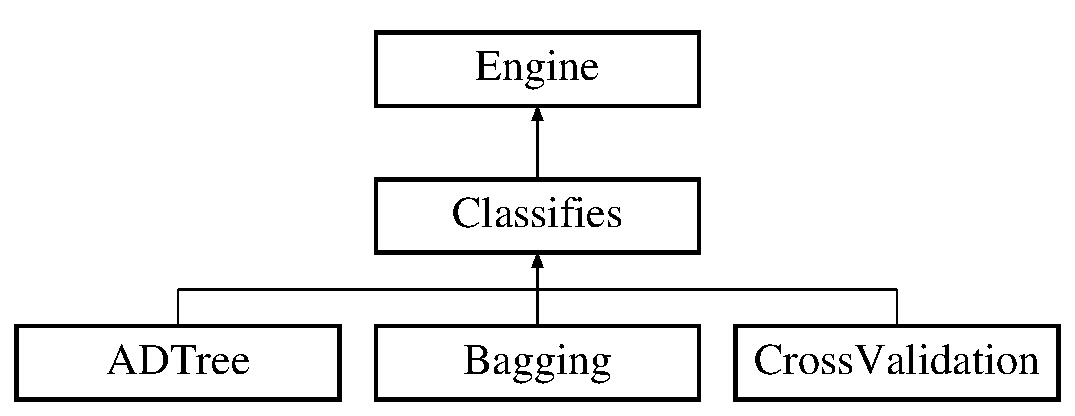
\includegraphics[height=3cm]{classClassifies}
\end{center}
\end{figure}
\subsection*{Public Member Functions}
\begin{DoxyCompactItemize}
\item 
virtual void \hyperlink{classClassifies_a15864d3a95edfde2bf48384c9b25c6d8}{classify} (int a\mbox{[}4\mbox{]})=0
\item 
virtual void \hyperlink{classClassifies_a7d2ae89f04af1a74eb6dd35be8eda476}{classify} (int a\mbox{[}4\mbox{]}, \hyperlink{classSnpData}{SnpData} $\ast$)=0
\item 
virtual int \hyperlink{classClassifies_a5e3d218b44024ec2c3ab3398e3dbd2e3}{classify} (vector$<$ short $>$ \&)=0
\end{DoxyCompactItemize}


\subsection{Detailed Description}
Abstract class for an engine that can be used in a bag or under cross-\/validation.

The point here is to include the capacity for classifying instances.

An engine is a large algorithm class like SNPGWA, INTERTWOLOG, ADTREE, or ADTREEBAG 

\subsection{Member Function Documentation}
\hypertarget{classClassifies_a5e3d218b44024ec2c3ab3398e3dbd2e3}{
\index{Classifies@{Classifies}!classify@{classify}}
\index{classify@{classify}!Classifies@{Classifies}}
\subsubsection[{classify}]{\setlength{\rightskip}{0pt plus 5cm}virtual int Classifies::classify (vector$<$ short $>$ \&)\hspace{0.3cm}{\ttfamily  \mbox{[}pure virtual\mbox{]}}}}
\label{classClassifies_a5e3d218b44024ec2c3ab3398e3dbd2e3}


Implemented in \hyperlink{classADTree_a266a816ec8750b5ceb1549ff610fb67b}{ADTree}, \hyperlink{classBagging_a92072d6610e9b9d932d10a123cc6ff18}{Bagging}, and \hyperlink{classCrossValidation_a4c11570314fe9e98e434abee990ac2d4}{CrossValidation}.

\hypertarget{classClassifies_a7d2ae89f04af1a74eb6dd35be8eda476}{
\index{Classifies@{Classifies}!classify@{classify}}
\index{classify@{classify}!Classifies@{Classifies}}
\subsubsection[{classify}]{\setlength{\rightskip}{0pt plus 5cm}virtual void Classifies::classify (int {\em a}\mbox{[}4\mbox{]}, \/  {\bf SnpData} $\ast$)\hspace{0.3cm}{\ttfamily  \mbox{[}pure virtual\mbox{]}}}}
\label{classClassifies_a7d2ae89f04af1a74eb6dd35be8eda476}


Implemented in \hyperlink{classADTree_a498b7a7830dba60118e89d5f5bb7cbd3}{ADTree}, \hyperlink{classBagging_a9b17e15983996f8ae3b39564e7c3deba}{Bagging}, and \hyperlink{classCrossValidation_a237cd67d2e1e6fc7c62abf0fef8bd3e8}{CrossValidation}.

\hypertarget{classClassifies_a15864d3a95edfde2bf48384c9b25c6d8}{
\index{Classifies@{Classifies}!classify@{classify}}
\index{classify@{classify}!Classifies@{Classifies}}
\subsubsection[{classify}]{\setlength{\rightskip}{0pt plus 5cm}virtual void Classifies::classify (int {\em a}\mbox{[}4\mbox{]})\hspace{0.3cm}{\ttfamily  \mbox{[}pure virtual\mbox{]}}}}
\label{classClassifies_a15864d3a95edfde2bf48384c9b25c6d8}


Implemented in \hyperlink{classADTree_a335cdf83f845638ae6c74fa1d7e7e4b8}{ADTree}, \hyperlink{classBagging_a02227120bc610a21f39f2454ac03ec7b}{Bagging}, and \hyperlink{classCrossValidation_a6b26e9c496dac46fb066fae0f381fed0}{CrossValidation}.



The documentation for this class was generated from the following file:\begin{DoxyCompactItemize}
\item 
engine/\hyperlink{combinable_8h}{combinable.h}\end{DoxyCompactItemize}

\hypertarget{classCondition}{
\section{Condition Class Reference}
\label{classCondition}\index{Condition@{Condition}}
}


{\ttfamily \#include $<$condition.h$>$}

\subsection*{Public Types}
\begin{DoxyCompactItemize}
\item 
enum \hyperlink{classCondition_af41afbd9545b1fb2e2cb4a4792d52408}{comparison} \{ \par
\hyperlink{classCondition_af41afbd9545b1fb2e2cb4a4792d52408a7bdd26a389de897c518f2e7c47c9b9fa}{GE}, 
\hyperlink{classCondition_af41afbd9545b1fb2e2cb4a4792d52408ab0e581f3ae4b7a4ae2f77a3448c3ae73}{GT}, 
\hyperlink{classCondition_af41afbd9545b1fb2e2cb4a4792d52408ab3b023e6fa08cc0029192012b5a9846c}{LE}, 
\hyperlink{classCondition_af41afbd9545b1fb2e2cb4a4792d52408a852b6dd7b2dd782a2bde9d8d80a822d6}{LT}, 
\par
\hyperlink{classCondition_af41afbd9545b1fb2e2cb4a4792d52408a19ca99ac1f587159a6a170f37c22626d}{EQ}, 
\hyperlink{classCondition_af41afbd9545b1fb2e2cb4a4792d52408ab5f11e0e13fa4dea2863922a39e921f3}{NE}
 \}
\end{DoxyCompactItemize}
\subsection*{Public Member Functions}
\begin{DoxyCompactItemize}
\item 
\hyperlink{classCondition_af11513db4fcbde93961fa0b65e7ab764}{Condition} ()
\item 
bool \hyperlink{classCondition_a332c47202b299556963b3a68b050d3b9}{evaluate} (vector$<$ short $>$ $\ast$)
\item 
void \hyperlink{classCondition_a6f95eacf1437f7800ebf81c89a6cf6c0}{inverse} ()
\item 
string \hyperlink{classCondition_a00c6f9ba842c26e21bba25848f2b0404}{print} (\hyperlink{classDataAccess}{DataAccess} $\ast$data)
\item 
string \hyperlink{classCondition_a8307a156ebd3e09433f30bf9975f60d6}{print\_\-reverse} (\hyperlink{classDataAccess}{DataAccess} $\ast$data)
\item 
string \hyperlink{classCondition_a2139d8d1ae38b2ca9dfea947b3f6f858}{hash} ()
\item 
int \hyperlink{classCondition_ad4c38e1ab62b02a54cec27b36d957c21}{operator==} (const \hyperlink{classCondition}{Condition} \&right)
\end{DoxyCompactItemize}
\subsection*{Data Fields}
\begin{DoxyCompactItemize}
\item 
long \hyperlink{classCondition_a081912e5b4f419de020299acbc8ee760}{attribute\_\-index}
\item 
\hyperlink{classCondition_af41afbd9545b1fb2e2cb4a4792d52408}{comparison} \hyperlink{classCondition_afe18e96245b5ebaa6bf8318ec9184d82}{genotype\_\-conditional}
\item 
short \hyperlink{classCondition_a11cbb60b2a8ee2446b10f0dc8858cfae}{genotype\_\-reference}
\end{DoxyCompactItemize}


\subsection{Member Enumeration Documentation}
\hypertarget{classCondition_af41afbd9545b1fb2e2cb4a4792d52408}{
\index{Condition@{Condition}!comparison@{comparison}}
\index{comparison@{comparison}!Condition@{Condition}}
\subsubsection[{comparison}]{\setlength{\rightskip}{0pt plus 5cm}enum {\bf Condition::comparison}}}
\label{classCondition_af41afbd9545b1fb2e2cb4a4792d52408}
\begin{Desc}
\item[Enumerator: ]\par
\begin{description}
\index{GE@{GE}!Condition@{Condition}}\index{Condition@{Condition}!GE@{GE}}\item[{\em 
\hypertarget{classCondition_af41afbd9545b1fb2e2cb4a4792d52408a7bdd26a389de897c518f2e7c47c9b9fa}{
GE}
\label{classCondition_af41afbd9545b1fb2e2cb4a4792d52408a7bdd26a389de897c518f2e7c47c9b9fa}
}]\index{GT@{GT}!Condition@{Condition}}\index{Condition@{Condition}!GT@{GT}}\item[{\em 
\hypertarget{classCondition_af41afbd9545b1fb2e2cb4a4792d52408ab0e581f3ae4b7a4ae2f77a3448c3ae73}{
GT}
\label{classCondition_af41afbd9545b1fb2e2cb4a4792d52408ab0e581f3ae4b7a4ae2f77a3448c3ae73}
}]\index{LE@{LE}!Condition@{Condition}}\index{Condition@{Condition}!LE@{LE}}\item[{\em 
\hypertarget{classCondition_af41afbd9545b1fb2e2cb4a4792d52408ab3b023e6fa08cc0029192012b5a9846c}{
LE}
\label{classCondition_af41afbd9545b1fb2e2cb4a4792d52408ab3b023e6fa08cc0029192012b5a9846c}
}]\index{LT@{LT}!Condition@{Condition}}\index{Condition@{Condition}!LT@{LT}}\item[{\em 
\hypertarget{classCondition_af41afbd9545b1fb2e2cb4a4792d52408a852b6dd7b2dd782a2bde9d8d80a822d6}{
LT}
\label{classCondition_af41afbd9545b1fb2e2cb4a4792d52408a852b6dd7b2dd782a2bde9d8d80a822d6}
}]\index{EQ@{EQ}!Condition@{Condition}}\index{Condition@{Condition}!EQ@{EQ}}\item[{\em 
\hypertarget{classCondition_af41afbd9545b1fb2e2cb4a4792d52408a19ca99ac1f587159a6a170f37c22626d}{
EQ}
\label{classCondition_af41afbd9545b1fb2e2cb4a4792d52408a19ca99ac1f587159a6a170f37c22626d}
}]\index{NE@{NE}!Condition@{Condition}}\index{Condition@{Condition}!NE@{NE}}\item[{\em 
\hypertarget{classCondition_af41afbd9545b1fb2e2cb4a4792d52408ab5f11e0e13fa4dea2863922a39e921f3}{
NE}
\label{classCondition_af41afbd9545b1fb2e2cb4a4792d52408ab5f11e0e13fa4dea2863922a39e921f3}
}]\end{description}
\end{Desc}



\subsection{Constructor \& Destructor Documentation}
\hypertarget{classCondition_af11513db4fcbde93961fa0b65e7ab764}{
\index{Condition@{Condition}!Condition@{Condition}}
\index{Condition@{Condition}!Condition@{Condition}}
\subsubsection[{Condition}]{\setlength{\rightskip}{0pt plus 5cm}Condition::Condition ()}}
\label{classCondition_af11513db4fcbde93961fa0b65e7ab764}


\subsection{Member Function Documentation}
\hypertarget{classCondition_a332c47202b299556963b3a68b050d3b9}{
\index{Condition@{Condition}!evaluate@{evaluate}}
\index{evaluate@{evaluate}!Condition@{Condition}}
\subsubsection[{evaluate}]{\setlength{\rightskip}{0pt plus 5cm}bool Condition::evaluate (vector$<$ short $>$ $\ast$ {\em vec})}}
\label{classCondition_a332c47202b299556963b3a68b050d3b9}
Actually evaluate a condition given the data in vector

Returns: the boolean value for this \hyperlink{classCondition}{Condition} on this data. \hypertarget{classCondition_a2139d8d1ae38b2ca9dfea947b3f6f858}{
\index{Condition@{Condition}!hash@{hash}}
\index{hash@{hash}!Condition@{Condition}}
\subsubsection[{hash}]{\setlength{\rightskip}{0pt plus 5cm}string Condition::hash ()}}
\label{classCondition_a2139d8d1ae38b2ca9dfea947b3f6f858}
\hypertarget{classCondition_a6f95eacf1437f7800ebf81c89a6cf6c0}{
\index{Condition@{Condition}!inverse@{inverse}}
\index{inverse@{inverse}!Condition@{Condition}}
\subsubsection[{inverse}]{\setlength{\rightskip}{0pt plus 5cm}void Condition::inverse ()}}
\label{classCondition_a6f95eacf1437f7800ebf81c89a6cf6c0}
Switch the sign of the conditional to its opposite \hypertarget{classCondition_ad4c38e1ab62b02a54cec27b36d957c21}{
\index{Condition@{Condition}!operator==@{operator==}}
\index{operator==@{operator==}!Condition@{Condition}}
\subsubsection[{operator==}]{\setlength{\rightskip}{0pt plus 5cm}int Condition::operator== (const {\bf Condition} \& {\em right})}}
\label{classCondition_ad4c38e1ab62b02a54cec27b36d957c21}
Check for equality of all parts of the condition.

\begin{DoxyReturn}{Returns}
int 1 if equal, 0 otherwise 
\end{DoxyReturn}
\hypertarget{classCondition_a00c6f9ba842c26e21bba25848f2b0404}{
\index{Condition@{Condition}!print@{print}}
\index{print@{print}!Condition@{Condition}}
\subsubsection[{print}]{\setlength{\rightskip}{0pt plus 5cm}string Condition::print ({\bf DataAccess} $\ast$ {\em data})}}
\label{classCondition_a00c6f9ba842c26e21bba25848f2b0404}
Return a formatted string.

TODO: consider changing to to\_\-string

\begin{DoxyReturn}{Returns}
string representation of the condition. 
\end{DoxyReturn}
\hypertarget{classCondition_a8307a156ebd3e09433f30bf9975f60d6}{
\index{Condition@{Condition}!print\_\-reverse@{print\_\-reverse}}
\index{print\_\-reverse@{print\_\-reverse}!Condition@{Condition}}
\subsubsection[{print\_\-reverse}]{\setlength{\rightskip}{0pt plus 5cm}string Condition::print\_\-reverse ({\bf DataAccess} $\ast$ {\em data})}}
\label{classCondition_a8307a156ebd3e09433f30bf9975f60d6}


\subsection{Field Documentation}
\hypertarget{classCondition_a081912e5b4f419de020299acbc8ee760}{
\index{Condition@{Condition}!attribute\_\-index@{attribute\_\-index}}
\index{attribute\_\-index@{attribute\_\-index}!Condition@{Condition}}
\subsubsection[{attribute\_\-index}]{\setlength{\rightskip}{0pt plus 5cm}long {\bf Condition::attribute\_\-index}}}
\label{classCondition_a081912e5b4f419de020299acbc8ee760}
\hypertarget{classCondition_afe18e96245b5ebaa6bf8318ec9184d82}{
\index{Condition@{Condition}!genotype\_\-conditional@{genotype\_\-conditional}}
\index{genotype\_\-conditional@{genotype\_\-conditional}!Condition@{Condition}}
\subsubsection[{genotype\_\-conditional}]{\setlength{\rightskip}{0pt plus 5cm}{\bf comparison} {\bf Condition::genotype\_\-conditional}}}
\label{classCondition_afe18e96245b5ebaa6bf8318ec9184d82}
\hypertarget{classCondition_a11cbb60b2a8ee2446b10f0dc8858cfae}{
\index{Condition@{Condition}!genotype\_\-reference@{genotype\_\-reference}}
\index{genotype\_\-reference@{genotype\_\-reference}!Condition@{Condition}}
\subsubsection[{genotype\_\-reference}]{\setlength{\rightskip}{0pt plus 5cm}short {\bf Condition::genotype\_\-reference}}}
\label{classCondition_a11cbb60b2a8ee2446b10f0dc8858cfae}


The documentation for this class was generated from the following files:\begin{DoxyCompactItemize}
\item 
engine/adtree/\hyperlink{condition_8h}{condition.h}\item 
engine/adtree/\hyperlink{condition_8cpp}{condition.cpp}\end{DoxyCompactItemize}

\hypertarget{classConditionNumberEx}{
\section{ConditionNumberEx Class Reference}
\label{classConditionNumberEx}\index{ConditionNumberEx@{ConditionNumberEx}}
}


{\ttfamily \#include $<$exceptions.h$>$}

Inheritance diagram for ConditionNumberEx:\begin{figure}[H]
\begin{center}
\leavevmode
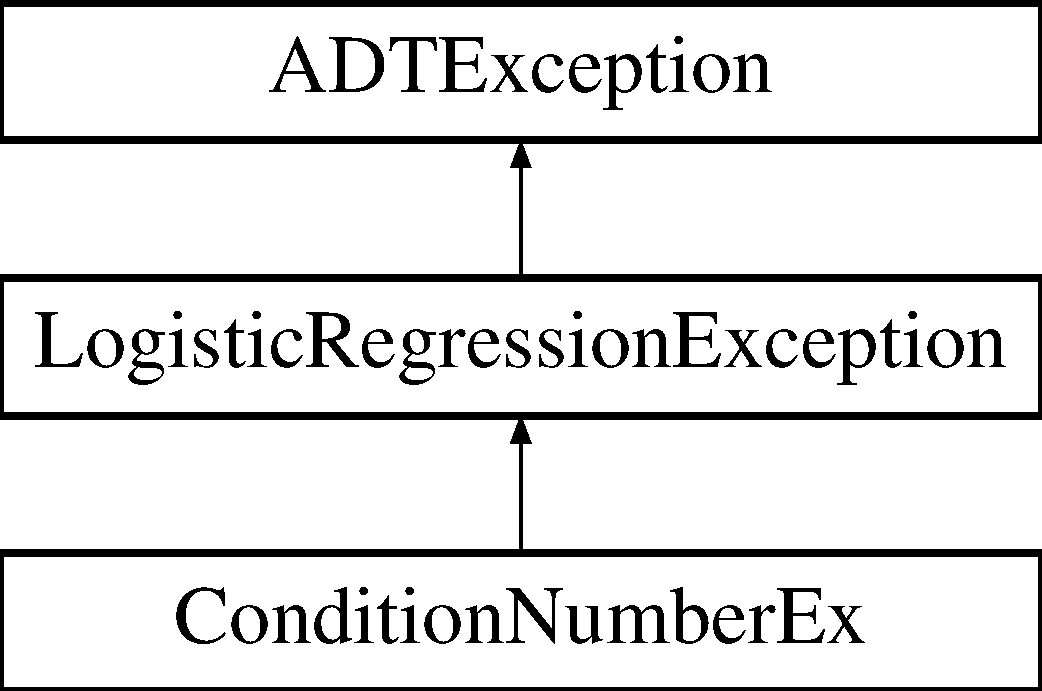
\includegraphics[height=3cm]{classConditionNumberEx}
\end{center}
\end{figure}


The documentation for this class was generated from the following file:\begin{DoxyCompactItemize}
\item 
engine/utils/\hyperlink{exceptions_8h}{exceptions.h}\end{DoxyCompactItemize}

\hypertarget{classContGenoStats}{
\section{ContGenoStats Class Reference}
\label{classContGenoStats}\index{ContGenoStats@{ContGenoStats}}
}


{\ttfamily \#include $<$cont\_\-genostats.hh$>$}

\subsection*{Data Structures}
\begin{DoxyCompactItemize}
\item 
struct \hyperlink{structContGenoStats_1_1statisticsOutput}{statisticsOutput}
\end{DoxyCompactItemize}
\subsection*{Public Member Functions}
\begin{DoxyCompactItemize}
\item 
\hyperlink{classContGenoStats_a63e8c1b4f83723b05dfc7be462b438dc}{ContGenoStats} (\hyperlink{classDataAccess}{DataAccess} $\ast$d)
\item 
void \hyperlink{classContGenoStats_a4b6add4b82e3f7b49594007e8de252e2}{prepGenoStatsForOutput} (int snp, \hyperlink{structContGenoStatsResults}{ContGenoStatsResults} \&results)
\end{DoxyCompactItemize}
\subsection*{Protected Member Functions}
\begin{DoxyCompactItemize}
\item 
double \hyperlink{classContGenoStats_aac4cebdec0c08a7a713ed31486e84404}{sumSquaresTotal} (vector$<$ double $>$ response)
\item 
void \hyperlink{classContGenoStats_a4e2fbf202fe9a14fa9130ac4486674f5}{computeMeanAndSD} (int snp, \hyperlink{structContGenoStatsResults}{ContGenoStatsResults} \&results)
\item 
void \hyperlink{classContGenoStats_abf83f07dacc05fa98f45c53bccc8489d}{computeLinRegStats} (int snp, \hyperlink{structContGenoStatsResults}{ContGenoStatsResults} \&results)
\item 
void \hyperlink{classContGenoStats_a19a72ee3254feaf596fde9b4f0446647}{computeLackOfFit} (int snp, \hyperlink{structContGenoStatsResults}{ContGenoStatsResults} \&results)
\item 
\hyperlink{structContGenoStats_1_1statisticsOutput}{statisticsOutput} \hyperlink{classContGenoStats_a5bf2b6b904d77644a1e76eadbac9865a}{computeSingleStats} (const vector$<$ vector$<$ double $>$ $>$ \&input, const vector$<$ double $>$ \&response, double meanResponse, string message, int snp)
\item 
void \hyperlink{classContGenoStats_a7a75df670c1ee712c09255c3f4954961}{covariateAdjust} (int snp)
\item 
void \hyperlink{classContGenoStats_abd30393de9c715bf4613f917130617ef}{blankLinRegStats} (\hyperlink{structContGenoStatsResults}{ContGenoStatsResults} \&results)
\end{DoxyCompactItemize}
\subsection*{Protected Attributes}
\begin{DoxyCompactItemize}
\item 
\hyperlink{classDataAccess}{DataAccess} $\ast$ \hyperlink{classContGenoStats_a3e0477a12dd35807fa4e1335d8119a5d}{data}
\item 
double \hyperlink{classContGenoStats_acc4ad5538332d2b491c5526145a49fbe}{responseMean}
\item 
bool \hyperlink{classContGenoStats_ad1e33f4b7b4137273099df0d7dcbdb4d}{ranMeans}
\item 
double \hyperlink{classContGenoStats_a7dca7abc1d8302920600dd40a892b249}{meanResidual}
\item 
vector$<$ double $>$ \hyperlink{classContGenoStats_ace549196ed683fba9cd205a240ec552b}{residuals}
\end{DoxyCompactItemize}


\subsection{Constructor \& Destructor Documentation}
\hypertarget{classContGenoStats_a63e8c1b4f83723b05dfc7be462b438dc}{
\index{ContGenoStats@{ContGenoStats}!ContGenoStats@{ContGenoStats}}
\index{ContGenoStats@{ContGenoStats}!ContGenoStats@{ContGenoStats}}
\subsubsection[{ContGenoStats}]{\setlength{\rightskip}{0pt plus 5cm}ContGenoStats::ContGenoStats ({\bf DataAccess} $\ast$ {\em d})}}
\label{classContGenoStats_a63e8c1b4f83723b05dfc7be462b438dc}


\subsection{Member Function Documentation}
\hypertarget{classContGenoStats_abd30393de9c715bf4613f917130617ef}{
\index{ContGenoStats@{ContGenoStats}!blankLinRegStats@{blankLinRegStats}}
\index{blankLinRegStats@{blankLinRegStats}!ContGenoStats@{ContGenoStats}}
\subsubsection[{blankLinRegStats}]{\setlength{\rightskip}{0pt plus 5cm}void ContGenoStats::blankLinRegStats ({\bf ContGenoStatsResults} \& {\em results})\hspace{0.3cm}{\ttfamily  \mbox{[}protected\mbox{]}}}}
\label{classContGenoStats_abd30393de9c715bf4613f917130617ef}
Default all pvals, se, and betas.


\begin{DoxyParams}{Parameters}
\item[{\em results}]A Genostats results struct that we will turn to all default values. \end{DoxyParams}
\hypertarget{classContGenoStats_a19a72ee3254feaf596fde9b4f0446647}{
\index{ContGenoStats@{ContGenoStats}!computeLackOfFit@{computeLackOfFit}}
\index{computeLackOfFit@{computeLackOfFit}!ContGenoStats@{ContGenoStats}}
\subsubsection[{computeLackOfFit}]{\setlength{\rightskip}{0pt plus 5cm}void ContGenoStats::computeLackOfFit (int {\em snp}, \/  {\bf ContGenoStatsResults} \& {\em results})\hspace{0.3cm}{\ttfamily  \mbox{[}protected\mbox{]}}}}
\label{classContGenoStats_a19a72ee3254feaf596fde9b4f0446647}
Compute the lack of fit test statistic.


\begin{DoxyParams}{Parameters}
\item[{\em snp}]The SNP index. \item[{\em results}]The stats results object that will hold the response. \end{DoxyParams}
\hypertarget{classContGenoStats_abf83f07dacc05fa98f45c53bccc8489d}{
\index{ContGenoStats@{ContGenoStats}!computeLinRegStats@{computeLinRegStats}}
\index{computeLinRegStats@{computeLinRegStats}!ContGenoStats@{ContGenoStats}}
\subsubsection[{computeLinRegStats}]{\setlength{\rightskip}{0pt plus 5cm}void ContGenoStats::computeLinRegStats (int {\em snp}, \/  {\bf ContGenoStatsResults} \& {\em results})\hspace{0.3cm}{\ttfamily  \mbox{[}protected\mbox{]}}}}
\label{classContGenoStats_abf83f07dacc05fa98f45c53bccc8489d}
Use the linear regression engine to compute statistics beta SE p-\/val \hypertarget{classContGenoStats_a4e2fbf202fe9a14fa9130ac4486674f5}{
\index{ContGenoStats@{ContGenoStats}!computeMeanAndSD@{computeMeanAndSD}}
\index{computeMeanAndSD@{computeMeanAndSD}!ContGenoStats@{ContGenoStats}}
\subsubsection[{computeMeanAndSD}]{\setlength{\rightskip}{0pt plus 5cm}void ContGenoStats::computeMeanAndSD (int {\em snp}, \/  {\bf ContGenoStatsResults} \& {\em results})\hspace{0.3cm}{\ttfamily  \mbox{[}protected\mbox{]}}}}
\label{classContGenoStats_a4e2fbf202fe9a14fa9130ac4486674f5}
Compute the mean and standard deviation statistics for the following groups of individuals:

AA,Aa,aa,AA/Aa,Aa/aa \hypertarget{classContGenoStats_a5bf2b6b904d77644a1e76eadbac9865a}{
\index{ContGenoStats@{ContGenoStats}!computeSingleStats@{computeSingleStats}}
\index{computeSingleStats@{computeSingleStats}!ContGenoStats@{ContGenoStats}}
\subsubsection[{computeSingleStats}]{\setlength{\rightskip}{0pt plus 5cm}{\bf ContGenoStats::statisticsOutput} ContGenoStats::computeSingleStats (const vector$<$ vector$<$ double $>$ $>$ \& {\em in}, \/  const vector$<$ double $>$ \& {\em response}, \/  double {\em meanResidual}, \/  string {\em failMessage}, \/  int {\em currentSNP})\hspace{0.3cm}{\ttfamily  \mbox{[}protected\mbox{]}}}}
\label{classContGenoStats_a5bf2b6b904d77644a1e76eadbac9865a}
Compute a single set of statistics including p\_\-val, beta, se.

NOTE: The pvalues ect will be reported based on the last beta. Order your variables accordingly.


\begin{DoxyParams}{Parameters}
\item[{\em in}]The input to LR engine \item[{\em response}]The response variables. \item[{\em meanResidual}]of the response variable \end{DoxyParams}
\begin{DoxyReturn}{Returns}
Struct with results for last beta. 
\end{DoxyReturn}
\hypertarget{classContGenoStats_a7a75df670c1ee712c09255c3f4954961}{
\index{ContGenoStats@{ContGenoStats}!covariateAdjust@{covariateAdjust}}
\index{covariateAdjust@{covariateAdjust}!ContGenoStats@{ContGenoStats}}
\subsubsection[{covariateAdjust}]{\setlength{\rightskip}{0pt plus 5cm}void ContGenoStats::covariateAdjust (int {\em snp})\hspace{0.3cm}{\ttfamily  \mbox{[}protected\mbox{]}}}}
\label{classContGenoStats_a7a75df670c1ee712c09255c3f4954961}
Fill the residuals column.

All other tests are designed to ignore covariates because they are preadjusted away here.

NOTE: The residuals are stored for all individuals in the data set for whom the current SNP's value is not 0. Therefore, it can be used directly rather than recomputed.


\begin{DoxyParams}{Parameters}
\item[{\em snp}]The SNP we are operating on. \end{DoxyParams}
\hypertarget{classContGenoStats_a4b6add4b82e3f7b49594007e8de252e2}{
\index{ContGenoStats@{ContGenoStats}!prepGenoStatsForOutput@{prepGenoStatsForOutput}}
\index{prepGenoStatsForOutput@{prepGenoStatsForOutput}!ContGenoStats@{ContGenoStats}}
\subsubsection[{prepGenoStatsForOutput}]{\setlength{\rightskip}{0pt plus 5cm}void ContGenoStats::prepGenoStatsForOutput (int {\em snp}, \/  {\bf ContGenoStatsResults} \& {\em results})}}
\label{classContGenoStats_a4b6add4b82e3f7b49594007e8de252e2}
Perform all genotypic association operations.

Makes heavy use of the linear regression and ANCOVA engines.

Calculates $\ast$ 2 df test $\ast$ dom, add, rec test $\ast$ means and variance for dom, rec groupings $\ast$ lof test

\begin{DoxyAuthor}{Author}
Richard T. Guy 
\end{DoxyAuthor}
\hypertarget{classContGenoStats_aac4cebdec0c08a7a713ed31486e84404}{
\index{ContGenoStats@{ContGenoStats}!sumSquaresTotal@{sumSquaresTotal}}
\index{sumSquaresTotal@{sumSquaresTotal}!ContGenoStats@{ContGenoStats}}
\subsubsection[{sumSquaresTotal}]{\setlength{\rightskip}{0pt plus 5cm}double ContGenoStats::sumSquaresTotal (vector$<$ double $>$ {\em response})\hspace{0.3cm}{\ttfamily  \mbox{[}protected\mbox{]}}}}
\label{classContGenoStats_aac4cebdec0c08a7a713ed31486e84404}
Return the total sum of squares. Equal to sum of norm of difference to mean. 

\subsection{Field Documentation}
\hypertarget{classContGenoStats_a3e0477a12dd35807fa4e1335d8119a5d}{
\index{ContGenoStats@{ContGenoStats}!data@{data}}
\index{data@{data}!ContGenoStats@{ContGenoStats}}
\subsubsection[{data}]{\setlength{\rightskip}{0pt plus 5cm}{\bf DataAccess}$\ast$ {\bf ContGenoStats::data}\hspace{0.3cm}{\ttfamily  \mbox{[}protected\mbox{]}}}}
\label{classContGenoStats_a3e0477a12dd35807fa4e1335d8119a5d}
\hypertarget{classContGenoStats_a7dca7abc1d8302920600dd40a892b249}{
\index{ContGenoStats@{ContGenoStats}!meanResidual@{meanResidual}}
\index{meanResidual@{meanResidual}!ContGenoStats@{ContGenoStats}}
\subsubsection[{meanResidual}]{\setlength{\rightskip}{0pt plus 5cm}double {\bf ContGenoStats::meanResidual}\hspace{0.3cm}{\ttfamily  \mbox{[}protected\mbox{]}}}}
\label{classContGenoStats_a7dca7abc1d8302920600dd40a892b249}
\hypertarget{classContGenoStats_ad1e33f4b7b4137273099df0d7dcbdb4d}{
\index{ContGenoStats@{ContGenoStats}!ranMeans@{ranMeans}}
\index{ranMeans@{ranMeans}!ContGenoStats@{ContGenoStats}}
\subsubsection[{ranMeans}]{\setlength{\rightskip}{0pt plus 5cm}bool {\bf ContGenoStats::ranMeans}\hspace{0.3cm}{\ttfamily  \mbox{[}protected\mbox{]}}}}
\label{classContGenoStats_ad1e33f4b7b4137273099df0d7dcbdb4d}
\hypertarget{classContGenoStats_ace549196ed683fba9cd205a240ec552b}{
\index{ContGenoStats@{ContGenoStats}!residuals@{residuals}}
\index{residuals@{residuals}!ContGenoStats@{ContGenoStats}}
\subsubsection[{residuals}]{\setlength{\rightskip}{0pt plus 5cm}vector$<$double$>$ {\bf ContGenoStats::residuals}\hspace{0.3cm}{\ttfamily  \mbox{[}protected\mbox{]}}}}
\label{classContGenoStats_ace549196ed683fba9cd205a240ec552b}
\hypertarget{classContGenoStats_acc4ad5538332d2b491c5526145a49fbe}{
\index{ContGenoStats@{ContGenoStats}!responseMean@{responseMean}}
\index{responseMean@{responseMean}!ContGenoStats@{ContGenoStats}}
\subsubsection[{responseMean}]{\setlength{\rightskip}{0pt plus 5cm}double {\bf ContGenoStats::responseMean}\hspace{0.3cm}{\ttfamily  \mbox{[}protected\mbox{]}}}}
\label{classContGenoStats_acc4ad5538332d2b491c5526145a49fbe}


The documentation for this class was generated from the following files:\begin{DoxyCompactItemize}
\item 
engine/qsnpgwa/\hyperlink{cont__genostats_8hh}{cont\_\-genostats.hh}\item 
engine/qsnpgwa/\hyperlink{cont__genostats_8cpp}{cont\_\-genostats.cpp}\end{DoxyCompactItemize}

\hypertarget{structContGenoStatsResults}{
\section{ContGenoStatsResults Struct Reference}
\label{structContGenoStatsResults}\index{ContGenoStatsResults@{ContGenoStatsResults}}
}


{\ttfamily \#include $<$qsnpgwa\_\-out.hh$>$}

\subsection*{Data Fields}
\begin{DoxyCompactItemize}
\item 
double \hyperlink{structContGenoStatsResults_a46e49f7e50c6e79cb72a24541af776de}{twodegfree\_\-pval}
\item 
double \hyperlink{structContGenoStatsResults_a960ab4eed8207be8ab943568f605f9e7}{add\_\-pval}
\item 
double \hyperlink{structContGenoStatsResults_a5697e46b20d7aad7a060867a62035c80}{add\_\-beta}
\item 
double \hyperlink{structContGenoStatsResults_ac62b2d1651db400043c51155fbe3e053}{add\_\-se}
\item 
double \hyperlink{structContGenoStatsResults_a62c4556a520da61125c52298d2b6fe14}{dom\_\-pval}
\item 
double \hyperlink{structContGenoStatsResults_a729b7ddee22418b46cd1952c1b39b204}{dom\_\-beta}
\item 
double \hyperlink{structContGenoStatsResults_a231a8457407e3c60a08542f5adb24186}{dom\_\-se}
\item 
double \hyperlink{structContGenoStatsResults_a6dea2a65a913691d67428a5bc7426a1b}{rec\_\-pval}
\item 
double \hyperlink{structContGenoStatsResults_a909674df22f15d550d6197074ce0412e}{rec\_\-beta}
\item 
double \hyperlink{structContGenoStatsResults_ae0b4b272bf7f6c40ab1cabd25fd84230}{rec\_\-se}
\item 
double \hyperlink{structContGenoStatsResults_a71916d32fe1bde64287e62116f87f8dd}{lof\_\-pval}
\item 
double \hyperlink{structContGenoStatsResults_a8c6a8778e17ebf6a14fdaf62a232d158}{meanAA}
\item 
double \hyperlink{structContGenoStatsResults_a17738d1319ce925127a86b45d321b58b}{sdAA}
\item 
double \hyperlink{structContGenoStatsResults_a190aa494b76da01c66207d8c3f2dd9f0}{meanAa}
\item 
double \hyperlink{structContGenoStatsResults_ac5f66a671f4a75a878a672ca9bcf6b89}{sdAa}
\item 
double \hyperlink{structContGenoStatsResults_ad583e064456319950eb63b0d5b4cd6dc}{meanaa}
\item 
double \hyperlink{structContGenoStatsResults_a2b3672ed884657068ae9963894d860c2}{sdaa}
\item 
double \hyperlink{structContGenoStatsResults_a46ef3b1678eac82e6866cc1d1f5b66e1}{meanAA\_\-Aa}
\item 
double \hyperlink{structContGenoStatsResults_a8d8428b3e5e541bc9f3ba97fe585ad1c}{sdAA\_\-Aa}
\item 
double \hyperlink{structContGenoStatsResults_af5f7eba4a16dc61a37b80c743ce32386}{meanAa\_\-aa}
\item 
double \hyperlink{structContGenoStatsResults_a334d91db43991eca160597eaefa1507f}{sdAa\_\-aa}
\item 
double \hyperlink{structContGenoStatsResults_a2116bd200a4104f32bd738dada6447f8}{rsquare}
\item 
double \hyperlink{structContGenoStatsResults_a3cf9bff725d092a36c17e999bebe9131}{dprime}
\end{DoxyCompactItemize}


\subsection{Field Documentation}
\hypertarget{structContGenoStatsResults_a5697e46b20d7aad7a060867a62035c80}{
\index{ContGenoStatsResults@{ContGenoStatsResults}!add\_\-beta@{add\_\-beta}}
\index{add\_\-beta@{add\_\-beta}!ContGenoStatsResults@{ContGenoStatsResults}}
\subsubsection[{add\_\-beta}]{\setlength{\rightskip}{0pt plus 5cm}double {\bf ContGenoStatsResults::add\_\-beta}}}
\label{structContGenoStatsResults_a5697e46b20d7aad7a060867a62035c80}
\hypertarget{structContGenoStatsResults_a960ab4eed8207be8ab943568f605f9e7}{
\index{ContGenoStatsResults@{ContGenoStatsResults}!add\_\-pval@{add\_\-pval}}
\index{add\_\-pval@{add\_\-pval}!ContGenoStatsResults@{ContGenoStatsResults}}
\subsubsection[{add\_\-pval}]{\setlength{\rightskip}{0pt plus 5cm}double {\bf ContGenoStatsResults::add\_\-pval}}}
\label{structContGenoStatsResults_a960ab4eed8207be8ab943568f605f9e7}
\hypertarget{structContGenoStatsResults_ac62b2d1651db400043c51155fbe3e053}{
\index{ContGenoStatsResults@{ContGenoStatsResults}!add\_\-se@{add\_\-se}}
\index{add\_\-se@{add\_\-se}!ContGenoStatsResults@{ContGenoStatsResults}}
\subsubsection[{add\_\-se}]{\setlength{\rightskip}{0pt plus 5cm}double {\bf ContGenoStatsResults::add\_\-se}}}
\label{structContGenoStatsResults_ac62b2d1651db400043c51155fbe3e053}
\hypertarget{structContGenoStatsResults_a729b7ddee22418b46cd1952c1b39b204}{
\index{ContGenoStatsResults@{ContGenoStatsResults}!dom\_\-beta@{dom\_\-beta}}
\index{dom\_\-beta@{dom\_\-beta}!ContGenoStatsResults@{ContGenoStatsResults}}
\subsubsection[{dom\_\-beta}]{\setlength{\rightskip}{0pt plus 5cm}double {\bf ContGenoStatsResults::dom\_\-beta}}}
\label{structContGenoStatsResults_a729b7ddee22418b46cd1952c1b39b204}
\hypertarget{structContGenoStatsResults_a62c4556a520da61125c52298d2b6fe14}{
\index{ContGenoStatsResults@{ContGenoStatsResults}!dom\_\-pval@{dom\_\-pval}}
\index{dom\_\-pval@{dom\_\-pval}!ContGenoStatsResults@{ContGenoStatsResults}}
\subsubsection[{dom\_\-pval}]{\setlength{\rightskip}{0pt plus 5cm}double {\bf ContGenoStatsResults::dom\_\-pval}}}
\label{structContGenoStatsResults_a62c4556a520da61125c52298d2b6fe14}
\hypertarget{structContGenoStatsResults_a231a8457407e3c60a08542f5adb24186}{
\index{ContGenoStatsResults@{ContGenoStatsResults}!dom\_\-se@{dom\_\-se}}
\index{dom\_\-se@{dom\_\-se}!ContGenoStatsResults@{ContGenoStatsResults}}
\subsubsection[{dom\_\-se}]{\setlength{\rightskip}{0pt plus 5cm}double {\bf ContGenoStatsResults::dom\_\-se}}}
\label{structContGenoStatsResults_a231a8457407e3c60a08542f5adb24186}
\hypertarget{structContGenoStatsResults_a3cf9bff725d092a36c17e999bebe9131}{
\index{ContGenoStatsResults@{ContGenoStatsResults}!dprime@{dprime}}
\index{dprime@{dprime}!ContGenoStatsResults@{ContGenoStatsResults}}
\subsubsection[{dprime}]{\setlength{\rightskip}{0pt plus 5cm}double {\bf ContGenoStatsResults::dprime}}}
\label{structContGenoStatsResults_a3cf9bff725d092a36c17e999bebe9131}
\hypertarget{structContGenoStatsResults_a71916d32fe1bde64287e62116f87f8dd}{
\index{ContGenoStatsResults@{ContGenoStatsResults}!lof\_\-pval@{lof\_\-pval}}
\index{lof\_\-pval@{lof\_\-pval}!ContGenoStatsResults@{ContGenoStatsResults}}
\subsubsection[{lof\_\-pval}]{\setlength{\rightskip}{0pt plus 5cm}double {\bf ContGenoStatsResults::lof\_\-pval}}}
\label{structContGenoStatsResults_a71916d32fe1bde64287e62116f87f8dd}
\hypertarget{structContGenoStatsResults_ad583e064456319950eb63b0d5b4cd6dc}{
\index{ContGenoStatsResults@{ContGenoStatsResults}!meanaa@{meanaa}}
\index{meanaa@{meanaa}!ContGenoStatsResults@{ContGenoStatsResults}}
\subsubsection[{meanaa}]{\setlength{\rightskip}{0pt plus 5cm}double {\bf ContGenoStatsResults::meanaa}}}
\label{structContGenoStatsResults_ad583e064456319950eb63b0d5b4cd6dc}
\hypertarget{structContGenoStatsResults_a190aa494b76da01c66207d8c3f2dd9f0}{
\index{ContGenoStatsResults@{ContGenoStatsResults}!meanAa@{meanAa}}
\index{meanAa@{meanAa}!ContGenoStatsResults@{ContGenoStatsResults}}
\subsubsection[{meanAa}]{\setlength{\rightskip}{0pt plus 5cm}double {\bf ContGenoStatsResults::meanAa}}}
\label{structContGenoStatsResults_a190aa494b76da01c66207d8c3f2dd9f0}
\hypertarget{structContGenoStatsResults_a8c6a8778e17ebf6a14fdaf62a232d158}{
\index{ContGenoStatsResults@{ContGenoStatsResults}!meanAA@{meanAA}}
\index{meanAA@{meanAA}!ContGenoStatsResults@{ContGenoStatsResults}}
\subsubsection[{meanAA}]{\setlength{\rightskip}{0pt plus 5cm}double {\bf ContGenoStatsResults::meanAA}}}
\label{structContGenoStatsResults_a8c6a8778e17ebf6a14fdaf62a232d158}
\hypertarget{structContGenoStatsResults_af5f7eba4a16dc61a37b80c743ce32386}{
\index{ContGenoStatsResults@{ContGenoStatsResults}!meanAa\_\-aa@{meanAa\_\-aa}}
\index{meanAa\_\-aa@{meanAa\_\-aa}!ContGenoStatsResults@{ContGenoStatsResults}}
\subsubsection[{meanAa\_\-aa}]{\setlength{\rightskip}{0pt plus 5cm}double {\bf ContGenoStatsResults::meanAa\_\-aa}}}
\label{structContGenoStatsResults_af5f7eba4a16dc61a37b80c743ce32386}
\hypertarget{structContGenoStatsResults_a46ef3b1678eac82e6866cc1d1f5b66e1}{
\index{ContGenoStatsResults@{ContGenoStatsResults}!meanAA\_\-Aa@{meanAA\_\-Aa}}
\index{meanAA\_\-Aa@{meanAA\_\-Aa}!ContGenoStatsResults@{ContGenoStatsResults}}
\subsubsection[{meanAA\_\-Aa}]{\setlength{\rightskip}{0pt plus 5cm}double {\bf ContGenoStatsResults::meanAA\_\-Aa}}}
\label{structContGenoStatsResults_a46ef3b1678eac82e6866cc1d1f5b66e1}
\hypertarget{structContGenoStatsResults_a909674df22f15d550d6197074ce0412e}{
\index{ContGenoStatsResults@{ContGenoStatsResults}!rec\_\-beta@{rec\_\-beta}}
\index{rec\_\-beta@{rec\_\-beta}!ContGenoStatsResults@{ContGenoStatsResults}}
\subsubsection[{rec\_\-beta}]{\setlength{\rightskip}{0pt plus 5cm}double {\bf ContGenoStatsResults::rec\_\-beta}}}
\label{structContGenoStatsResults_a909674df22f15d550d6197074ce0412e}
\hypertarget{structContGenoStatsResults_a6dea2a65a913691d67428a5bc7426a1b}{
\index{ContGenoStatsResults@{ContGenoStatsResults}!rec\_\-pval@{rec\_\-pval}}
\index{rec\_\-pval@{rec\_\-pval}!ContGenoStatsResults@{ContGenoStatsResults}}
\subsubsection[{rec\_\-pval}]{\setlength{\rightskip}{0pt plus 5cm}double {\bf ContGenoStatsResults::rec\_\-pval}}}
\label{structContGenoStatsResults_a6dea2a65a913691d67428a5bc7426a1b}
\hypertarget{structContGenoStatsResults_ae0b4b272bf7f6c40ab1cabd25fd84230}{
\index{ContGenoStatsResults@{ContGenoStatsResults}!rec\_\-se@{rec\_\-se}}
\index{rec\_\-se@{rec\_\-se}!ContGenoStatsResults@{ContGenoStatsResults}}
\subsubsection[{rec\_\-se}]{\setlength{\rightskip}{0pt plus 5cm}double {\bf ContGenoStatsResults::rec\_\-se}}}
\label{structContGenoStatsResults_ae0b4b272bf7f6c40ab1cabd25fd84230}
\hypertarget{structContGenoStatsResults_a2116bd200a4104f32bd738dada6447f8}{
\index{ContGenoStatsResults@{ContGenoStatsResults}!rsquare@{rsquare}}
\index{rsquare@{rsquare}!ContGenoStatsResults@{ContGenoStatsResults}}
\subsubsection[{rsquare}]{\setlength{\rightskip}{0pt plus 5cm}double {\bf ContGenoStatsResults::rsquare}}}
\label{structContGenoStatsResults_a2116bd200a4104f32bd738dada6447f8}
\hypertarget{structContGenoStatsResults_a2b3672ed884657068ae9963894d860c2}{
\index{ContGenoStatsResults@{ContGenoStatsResults}!sdaa@{sdaa}}
\index{sdaa@{sdaa}!ContGenoStatsResults@{ContGenoStatsResults}}
\subsubsection[{sdaa}]{\setlength{\rightskip}{0pt plus 5cm}double {\bf ContGenoStatsResults::sdaa}}}
\label{structContGenoStatsResults_a2b3672ed884657068ae9963894d860c2}
\hypertarget{structContGenoStatsResults_ac5f66a671f4a75a878a672ca9bcf6b89}{
\index{ContGenoStatsResults@{ContGenoStatsResults}!sdAa@{sdAa}}
\index{sdAa@{sdAa}!ContGenoStatsResults@{ContGenoStatsResults}}
\subsubsection[{sdAa}]{\setlength{\rightskip}{0pt plus 5cm}double {\bf ContGenoStatsResults::sdAa}}}
\label{structContGenoStatsResults_ac5f66a671f4a75a878a672ca9bcf6b89}
\hypertarget{structContGenoStatsResults_a17738d1319ce925127a86b45d321b58b}{
\index{ContGenoStatsResults@{ContGenoStatsResults}!sdAA@{sdAA}}
\index{sdAA@{sdAA}!ContGenoStatsResults@{ContGenoStatsResults}}
\subsubsection[{sdAA}]{\setlength{\rightskip}{0pt plus 5cm}double {\bf ContGenoStatsResults::sdAA}}}
\label{structContGenoStatsResults_a17738d1319ce925127a86b45d321b58b}
\hypertarget{structContGenoStatsResults_a334d91db43991eca160597eaefa1507f}{
\index{ContGenoStatsResults@{ContGenoStatsResults}!sdAa\_\-aa@{sdAa\_\-aa}}
\index{sdAa\_\-aa@{sdAa\_\-aa}!ContGenoStatsResults@{ContGenoStatsResults}}
\subsubsection[{sdAa\_\-aa}]{\setlength{\rightskip}{0pt plus 5cm}double {\bf ContGenoStatsResults::sdAa\_\-aa}}}
\label{structContGenoStatsResults_a334d91db43991eca160597eaefa1507f}
\hypertarget{structContGenoStatsResults_a8d8428b3e5e541bc9f3ba97fe585ad1c}{
\index{ContGenoStatsResults@{ContGenoStatsResults}!sdAA\_\-Aa@{sdAA\_\-Aa}}
\index{sdAA\_\-Aa@{sdAA\_\-Aa}!ContGenoStatsResults@{ContGenoStatsResults}}
\subsubsection[{sdAA\_\-Aa}]{\setlength{\rightskip}{0pt plus 5cm}double {\bf ContGenoStatsResults::sdAA\_\-Aa}}}
\label{structContGenoStatsResults_a8d8428b3e5e541bc9f3ba97fe585ad1c}
\hypertarget{structContGenoStatsResults_a46e49f7e50c6e79cb72a24541af776de}{
\index{ContGenoStatsResults@{ContGenoStatsResults}!twodegfree\_\-pval@{twodegfree\_\-pval}}
\index{twodegfree\_\-pval@{twodegfree\_\-pval}!ContGenoStatsResults@{ContGenoStatsResults}}
\subsubsection[{twodegfree\_\-pval}]{\setlength{\rightskip}{0pt plus 5cm}double {\bf ContGenoStatsResults::twodegfree\_\-pval}}}
\label{structContGenoStatsResults_a46e49f7e50c6e79cb72a24541af776de}


The documentation for this struct was generated from the following file:\begin{DoxyCompactItemize}
\item 
engine/output/\hyperlink{qsnpgwa__out_8hh}{qsnpgwa\_\-out.hh}\end{DoxyCompactItemize}

\hypertarget{classContPopStats}{
\section{ContPopStats Class Reference}
\label{classContPopStats}\index{ContPopStats@{ContPopStats}}
}


{\ttfamily \#include $<$cont\_\-popstats.hh$>$}

\subsection*{Public Member Functions}
\begin{DoxyCompactItemize}
\item 
\hyperlink{classContPopStats_acca80293398e197b710f0b3087aa5a35}{ContPopStats} (\hyperlink{classDataAccess}{DataAccess} $\ast$d)
\item 
\hyperlink{classContPopStats_ae3a20e08cdc2e52ae52fb81fab5230f6}{$\sim$ContPopStats} ()
\item 
void \hyperlink{classContPopStats_a6af3b120a6775e035946fff299e4da1b}{prepPopStatsForOutput} (int snp, \hyperlink{structContPopStatsResults}{ContPopStatsResults} \&)
\end{DoxyCompactItemize}


\subsection{Constructor \& Destructor Documentation}
\hypertarget{classContPopStats_acca80293398e197b710f0b3087aa5a35}{
\index{ContPopStats@{ContPopStats}!ContPopStats@{ContPopStats}}
\index{ContPopStats@{ContPopStats}!ContPopStats@{ContPopStats}}
\subsubsection[{ContPopStats}]{\setlength{\rightskip}{0pt plus 5cm}ContPopStats::ContPopStats ({\bf DataAccess} $\ast$ {\em d})}}
\label{classContPopStats_acca80293398e197b710f0b3087aa5a35}
\hypertarget{classContPopStats_ae3a20e08cdc2e52ae52fb81fab5230f6}{
\index{ContPopStats@{ContPopStats}!$\sim$ContPopStats@{$\sim$ContPopStats}}
\index{$\sim$ContPopStats@{$\sim$ContPopStats}!ContPopStats@{ContPopStats}}
\subsubsection[{$\sim$ContPopStats}]{\setlength{\rightskip}{0pt plus 5cm}ContPopStats::$\sim$ContPopStats ()}}
\label{classContPopStats_ae3a20e08cdc2e52ae52fb81fab5230f6}


\subsection{Member Function Documentation}
\hypertarget{classContPopStats_a6af3b120a6775e035946fff299e4da1b}{
\index{ContPopStats@{ContPopStats}!prepPopStatsForOutput@{prepPopStatsForOutput}}
\index{prepPopStatsForOutput@{prepPopStatsForOutput}!ContPopStats@{ContPopStats}}
\subsubsection[{prepPopStatsForOutput}]{\setlength{\rightskip}{0pt plus 5cm}void ContPopStats::prepPopStatsForOutput (int {\em snp}, \/  {\bf ContPopStatsResults} \& {\em results})}}
\label{classContPopStats_a6af3b120a6775e035946fff299e4da1b}


The documentation for this class was generated from the following files:\begin{DoxyCompactItemize}
\item 
engine/qsnpgwa/\hyperlink{cont__popstats_8hh}{cont\_\-popstats.hh}\item 
engine/qsnpgwa/\hyperlink{cont__popstats_8cpp}{cont\_\-popstats.cpp}\end{DoxyCompactItemize}

\hypertarget{structContPopStatsResults}{
\section{ContPopStatsResults Struct Reference}
\label{structContPopStatsResults}\index{ContPopStatsResults@{ContPopStatsResults}}
}


{\ttfamily \#include $<$qsnpgwa\_\-out.hh$>$}

\subsection*{Data Fields}
\begin{DoxyCompactItemize}
\item 
int \hyperlink{structContPopStatsResults_a04ef963080d03327b6e6d1eebe843106}{totalIndiv}
\item 
double \hyperlink{structContPopStatsResults_a8297fa29146812547bfb1ac23ba80fd0}{maf}
\item 
double \hyperlink{structContPopStatsResults_a99338d04b0d1f0c6d53a934965bb027c}{perMissing}
\item 
double \hyperlink{structContPopStatsResults_a2f6fdbe9de430b4860ab85784061433b}{perMissingPVal}
\item 
int \hyperlink{structContPopStatsResults_a5438429a5e30beea5c49f3792999acb7}{numPP}
\item 
int \hyperlink{structContPopStatsResults_afb47561b968c5afb6c4e85c127b21460}{numPQ}
\item 
int \hyperlink{structContPopStatsResults_a5aa7545d6362d7ac90f5fc5b396fd61a}{numQQ}
\item 
double \hyperlink{structContPopStatsResults_a6826b4fdd5cc538a727706f4a1715c9f}{expPP}
\item 
double \hyperlink{structContPopStatsResults_a8b1e83d6fc7022b4cb21189c658d1b87}{expPQ}
\item 
double \hyperlink{structContPopStatsResults_a37ad35b704fb592c856fdd85b17edcc6}{expQQ}
\item 
double \hyperlink{structContPopStatsResults_afd4f2dc79e759ec94b523abe36c2b7e8}{chiSqPval}
\item 
double \hyperlink{structContPopStatsResults_af9e5a8c489fe6382b04b9164087ca2fc}{pHWE}
\end{DoxyCompactItemize}


\subsection{Field Documentation}
\hypertarget{structContPopStatsResults_afd4f2dc79e759ec94b523abe36c2b7e8}{
\index{ContPopStatsResults@{ContPopStatsResults}!chiSqPval@{chiSqPval}}
\index{chiSqPval@{chiSqPval}!ContPopStatsResults@{ContPopStatsResults}}
\subsubsection[{chiSqPval}]{\setlength{\rightskip}{0pt plus 5cm}double {\bf ContPopStatsResults::chiSqPval}}}
\label{structContPopStatsResults_afd4f2dc79e759ec94b523abe36c2b7e8}
\hypertarget{structContPopStatsResults_a6826b4fdd5cc538a727706f4a1715c9f}{
\index{ContPopStatsResults@{ContPopStatsResults}!expPP@{expPP}}
\index{expPP@{expPP}!ContPopStatsResults@{ContPopStatsResults}}
\subsubsection[{expPP}]{\setlength{\rightskip}{0pt plus 5cm}double {\bf ContPopStatsResults::expPP}}}
\label{structContPopStatsResults_a6826b4fdd5cc538a727706f4a1715c9f}
\hypertarget{structContPopStatsResults_a8b1e83d6fc7022b4cb21189c658d1b87}{
\index{ContPopStatsResults@{ContPopStatsResults}!expPQ@{expPQ}}
\index{expPQ@{expPQ}!ContPopStatsResults@{ContPopStatsResults}}
\subsubsection[{expPQ}]{\setlength{\rightskip}{0pt plus 5cm}double {\bf ContPopStatsResults::expPQ}}}
\label{structContPopStatsResults_a8b1e83d6fc7022b4cb21189c658d1b87}
\hypertarget{structContPopStatsResults_a37ad35b704fb592c856fdd85b17edcc6}{
\index{ContPopStatsResults@{ContPopStatsResults}!expQQ@{expQQ}}
\index{expQQ@{expQQ}!ContPopStatsResults@{ContPopStatsResults}}
\subsubsection[{expQQ}]{\setlength{\rightskip}{0pt plus 5cm}double {\bf ContPopStatsResults::expQQ}}}
\label{structContPopStatsResults_a37ad35b704fb592c856fdd85b17edcc6}
\hypertarget{structContPopStatsResults_a8297fa29146812547bfb1ac23ba80fd0}{
\index{ContPopStatsResults@{ContPopStatsResults}!maf@{maf}}
\index{maf@{maf}!ContPopStatsResults@{ContPopStatsResults}}
\subsubsection[{maf}]{\setlength{\rightskip}{0pt plus 5cm}double {\bf ContPopStatsResults::maf}}}
\label{structContPopStatsResults_a8297fa29146812547bfb1ac23ba80fd0}
\hypertarget{structContPopStatsResults_a5438429a5e30beea5c49f3792999acb7}{
\index{ContPopStatsResults@{ContPopStatsResults}!numPP@{numPP}}
\index{numPP@{numPP}!ContPopStatsResults@{ContPopStatsResults}}
\subsubsection[{numPP}]{\setlength{\rightskip}{0pt plus 5cm}int {\bf ContPopStatsResults::numPP}}}
\label{structContPopStatsResults_a5438429a5e30beea5c49f3792999acb7}
\hypertarget{structContPopStatsResults_afb47561b968c5afb6c4e85c127b21460}{
\index{ContPopStatsResults@{ContPopStatsResults}!numPQ@{numPQ}}
\index{numPQ@{numPQ}!ContPopStatsResults@{ContPopStatsResults}}
\subsubsection[{numPQ}]{\setlength{\rightskip}{0pt plus 5cm}int {\bf ContPopStatsResults::numPQ}}}
\label{structContPopStatsResults_afb47561b968c5afb6c4e85c127b21460}
\hypertarget{structContPopStatsResults_a5aa7545d6362d7ac90f5fc5b396fd61a}{
\index{ContPopStatsResults@{ContPopStatsResults}!numQQ@{numQQ}}
\index{numQQ@{numQQ}!ContPopStatsResults@{ContPopStatsResults}}
\subsubsection[{numQQ}]{\setlength{\rightskip}{0pt plus 5cm}int {\bf ContPopStatsResults::numQQ}}}
\label{structContPopStatsResults_a5aa7545d6362d7ac90f5fc5b396fd61a}
\hypertarget{structContPopStatsResults_a99338d04b0d1f0c6d53a934965bb027c}{
\index{ContPopStatsResults@{ContPopStatsResults}!perMissing@{perMissing}}
\index{perMissing@{perMissing}!ContPopStatsResults@{ContPopStatsResults}}
\subsubsection[{perMissing}]{\setlength{\rightskip}{0pt plus 5cm}double {\bf ContPopStatsResults::perMissing}}}
\label{structContPopStatsResults_a99338d04b0d1f0c6d53a934965bb027c}
\hypertarget{structContPopStatsResults_a2f6fdbe9de430b4860ab85784061433b}{
\index{ContPopStatsResults@{ContPopStatsResults}!perMissingPVal@{perMissingPVal}}
\index{perMissingPVal@{perMissingPVal}!ContPopStatsResults@{ContPopStatsResults}}
\subsubsection[{perMissingPVal}]{\setlength{\rightskip}{0pt plus 5cm}double {\bf ContPopStatsResults::perMissingPVal}}}
\label{structContPopStatsResults_a2f6fdbe9de430b4860ab85784061433b}
\hypertarget{structContPopStatsResults_af9e5a8c489fe6382b04b9164087ca2fc}{
\index{ContPopStatsResults@{ContPopStatsResults}!pHWE@{pHWE}}
\index{pHWE@{pHWE}!ContPopStatsResults@{ContPopStatsResults}}
\subsubsection[{pHWE}]{\setlength{\rightskip}{0pt plus 5cm}double {\bf ContPopStatsResults::pHWE}}}
\label{structContPopStatsResults_af9e5a8c489fe6382b04b9164087ca2fc}
\hypertarget{structContPopStatsResults_a04ef963080d03327b6e6d1eebe843106}{
\index{ContPopStatsResults@{ContPopStatsResults}!totalIndiv@{totalIndiv}}
\index{totalIndiv@{totalIndiv}!ContPopStatsResults@{ContPopStatsResults}}
\subsubsection[{totalIndiv}]{\setlength{\rightskip}{0pt plus 5cm}int {\bf ContPopStatsResults::totalIndiv}}}
\label{structContPopStatsResults_a04ef963080d03327b6e6d1eebe843106}


The documentation for this struct was generated from the following file:\begin{DoxyCompactItemize}
\item 
engine/output/\hyperlink{qsnpgwa__out_8hh}{qsnpgwa\_\-out.hh}\end{DoxyCompactItemize}

\hypertarget{classCrossValidation}{
\section{CrossValidation Class Reference}
\label{classCrossValidation}\index{CrossValidation@{CrossValidation}}
}


{\ttfamily \#include $<$cross\_\-val.h$>$}

Inheritance diagram for CrossValidation:\begin{figure}[H]
\begin{center}
\leavevmode
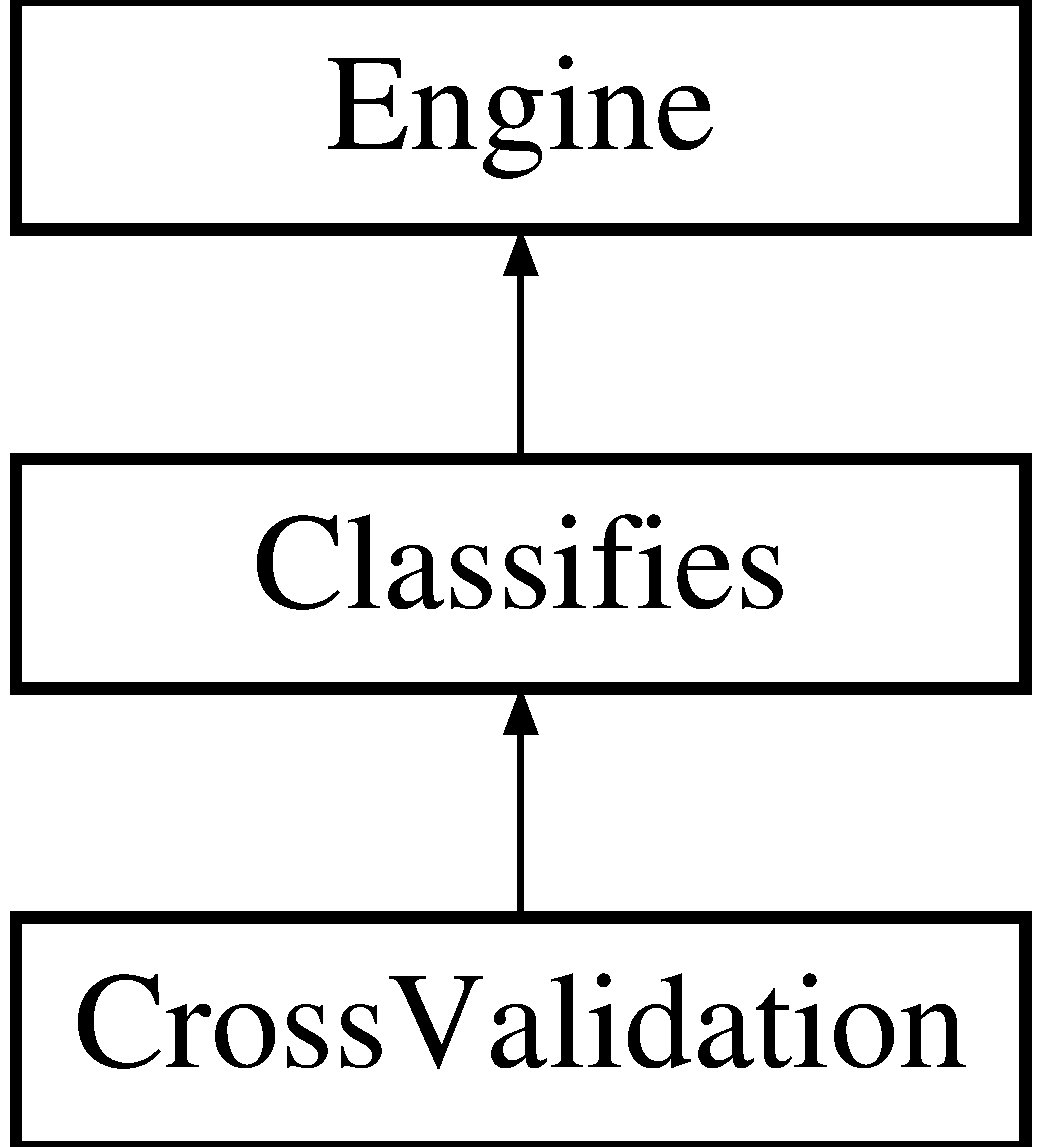
\includegraphics[height=3cm]{classCrossValidation}
\end{center}
\end{figure}
\subsection*{Public Member Functions}
\begin{DoxyCompactItemize}
\item 
\hyperlink{classCrossValidation_a855f538ef5541634f1dd94fbf965129b}{CrossValidation} ()
\item 
\hyperlink{classCrossValidation_a1e65ae700add864f2f85dcdf82940d74}{$\sim$CrossValidation} ()
\item 
virtual void \hyperlink{classCrossValidation_acf88bf85dec8d27f6aa97d9ec04ccf26}{init} ()
\begin{DoxyCompactList}\small\item\em From engine. \item\end{DoxyCompactList}\item 
virtual void \hyperlink{classCrossValidation_ad45dad478f034a39696660d7c93b34fa}{preProcess} ()
\item 
virtual void \hyperlink{classCrossValidation_a3435a227d91e03af7d1df7e2c6c4fce9}{process} ()
\item 
virtual void \hyperlink{classCrossValidation_a50b65a606c324404de92f44dba655154}{enslave} (\hyperlink{classEngineParamReader}{EngineParamReader} $\ast$)
\item 
virtual void \hyperlink{classCrossValidation_a1b4664d9123d676b778ff0e89379a1ba}{test} ()
\item 
virtual void \hyperlink{classCrossValidation_a6b26e9c496dac46fb066fae0f381fed0}{classify} (int a\mbox{[}4\mbox{]})
\begin{DoxyCompactList}\small\item\em Classification. \item\end{DoxyCompactList}\item 
virtual void \hyperlink{classCrossValidation_a237cd67d2e1e6fc7c62abf0fef8bd3e8}{classify} (int a\mbox{[}4\mbox{]}, \hyperlink{classSnpData}{SnpData} $\ast$)
\item 
virtual int \hyperlink{classCrossValidation_a4c11570314fe9e98e434abee990ac2d4}{classify} (vector$<$ short $>$ \&)
\end{DoxyCompactItemize}


\subsection{Constructor \& Destructor Documentation}
\hypertarget{classCrossValidation_a855f538ef5541634f1dd94fbf965129b}{
\index{CrossValidation@{CrossValidation}!CrossValidation@{CrossValidation}}
\index{CrossValidation@{CrossValidation}!CrossValidation@{CrossValidation}}
\subsubsection[{CrossValidation}]{\setlength{\rightskip}{0pt plus 5cm}CrossValidation::CrossValidation ()\hspace{0.3cm}{\ttfamily  \mbox{[}explicit\mbox{]}}}}
\label{classCrossValidation_a855f538ef5541634f1dd94fbf965129b}
\hypertarget{classCrossValidation_a1e65ae700add864f2f85dcdf82940d74}{
\index{CrossValidation@{CrossValidation}!$\sim$CrossValidation@{$\sim$CrossValidation}}
\index{$\sim$CrossValidation@{$\sim$CrossValidation}!CrossValidation@{CrossValidation}}
\subsubsection[{$\sim$CrossValidation}]{\setlength{\rightskip}{0pt plus 5cm}CrossValidation::$\sim$CrossValidation ()\hspace{0.3cm}{\ttfamily  \mbox{[}inline\mbox{]}}}}
\label{classCrossValidation_a1e65ae700add864f2f85dcdf82940d74}


\subsection{Member Function Documentation}
\hypertarget{classCrossValidation_a4c11570314fe9e98e434abee990ac2d4}{
\index{CrossValidation@{CrossValidation}!classify@{classify}}
\index{classify@{classify}!CrossValidation@{CrossValidation}}
\subsubsection[{classify}]{\setlength{\rightskip}{0pt plus 5cm}int CrossValidation::classify (vector$<$ short $>$ \&)\hspace{0.3cm}{\ttfamily  \mbox{[}virtual\mbox{]}}}}
\label{classCrossValidation_a4c11570314fe9e98e434abee990ac2d4}


Implements \hyperlink{classClassifies_a5e3d218b44024ec2c3ab3398e3dbd2e3}{Classifies}.

\hypertarget{classCrossValidation_a237cd67d2e1e6fc7c62abf0fef8bd3e8}{
\index{CrossValidation@{CrossValidation}!classify@{classify}}
\index{classify@{classify}!CrossValidation@{CrossValidation}}
\subsubsection[{classify}]{\setlength{\rightskip}{0pt plus 5cm}void CrossValidation::classify (int {\em a}\mbox{[}4\mbox{]}, \/  {\bf SnpData} $\ast$)\hspace{0.3cm}{\ttfamily  \mbox{[}virtual\mbox{]}}}}
\label{classCrossValidation_a237cd67d2e1e6fc7c62abf0fef8bd3e8}


Implements \hyperlink{classClassifies_a7d2ae89f04af1a74eb6dd35be8eda476}{Classifies}.

\hypertarget{classCrossValidation_a6b26e9c496dac46fb066fae0f381fed0}{
\index{CrossValidation@{CrossValidation}!classify@{classify}}
\index{classify@{classify}!CrossValidation@{CrossValidation}}
\subsubsection[{classify}]{\setlength{\rightskip}{0pt plus 5cm}void CrossValidation::classify (int {\em a}\mbox{[}4\mbox{]})\hspace{0.3cm}{\ttfamily  \mbox{[}virtual\mbox{]}}}}
\label{classCrossValidation_a6b26e9c496dac46fb066fae0f381fed0}


Classification. 

Report classification, which was precomputed. 

Implements \hyperlink{classClassifies_a15864d3a95edfde2bf48384c9b25c6d8}{Classifies}.

\hypertarget{classCrossValidation_a50b65a606c324404de92f44dba655154}{
\index{CrossValidation@{CrossValidation}!enslave@{enslave}}
\index{enslave@{enslave}!CrossValidation@{CrossValidation}}
\subsubsection[{enslave}]{\setlength{\rightskip}{0pt plus 5cm}void CrossValidation::enslave ({\bf EngineParamReader} $\ast$ {\em b})\hspace{0.3cm}{\ttfamily  \mbox{[}virtual\mbox{]}}}}
\label{classCrossValidation_a50b65a606c324404de92f44dba655154}
Make this engine controllable by another. 

Implements \hyperlink{classEngine_a023e094182312b1732fe53754c2fe5cb}{Engine}.

\hypertarget{classCrossValidation_acf88bf85dec8d27f6aa97d9ec04ccf26}{
\index{CrossValidation@{CrossValidation}!init@{init}}
\index{init@{init}!CrossValidation@{CrossValidation}}
\subsubsection[{init}]{\setlength{\rightskip}{0pt plus 5cm}void CrossValidation::init ()\hspace{0.3cm}{\ttfamily  \mbox{[}virtual\mbox{]}}}}
\label{classCrossValidation_acf88bf85dec8d27f6aa97d9ec04ccf26}


From engine. 

Open the data and read it into the data class. $\ast$ 

Implements \hyperlink{classEngine_aaa054d596fb8ced6e3eb4bee208f8c3d}{Engine}.

\hypertarget{classCrossValidation_ad45dad478f034a39696660d7c93b34fa}{
\index{CrossValidation@{CrossValidation}!preProcess@{preProcess}}
\index{preProcess@{preProcess}!CrossValidation@{CrossValidation}}
\subsubsection[{preProcess}]{\setlength{\rightskip}{0pt plus 5cm}void CrossValidation::preProcess ()\hspace{0.3cm}{\ttfamily  \mbox{[}virtual\mbox{]}}}}
\label{classCrossValidation_ad45dad478f034a39696660d7c93b34fa}
Create all of the engines and set up the master-\/slave system. Create data first. 

Implements \hyperlink{classEngine_aec7076b8979a13c96eceb362437dc68c}{Engine}.

\hypertarget{classCrossValidation_a3435a227d91e03af7d1df7e2c6c4fce9}{
\index{CrossValidation@{CrossValidation}!process@{process}}
\index{process@{process}!CrossValidation@{CrossValidation}}
\subsubsection[{process}]{\setlength{\rightskip}{0pt plus 5cm}void CrossValidation::process ()\hspace{0.3cm}{\ttfamily  \mbox{[}virtual\mbox{]}}}}
\label{classCrossValidation_a3435a227d91e03af7d1df7e2c6c4fce9}
Build a model on each of the cross-\/validation parts. Run the model on the left out individuals. Report individuals. 

Implements \hyperlink{classEngine_a005f8e277c3dea16ea05803fba223db7}{Engine}.

\hypertarget{classCrossValidation_a1b4664d9123d676b778ff0e89379a1ba}{
\index{CrossValidation@{CrossValidation}!test@{test}}
\index{test@{test}!CrossValidation@{CrossValidation}}
\subsubsection[{test}]{\setlength{\rightskip}{0pt plus 5cm}void CrossValidation::test ()\hspace{0.3cm}{\ttfamily  \mbox{[}virtual\mbox{]}}}}
\label{classCrossValidation_a1b4664d9123d676b778ff0e89379a1ba}


Implements \hyperlink{classEngine_a2927c4a4263809453063ad482c6434a4}{Engine}.



The documentation for this class was generated from the following files:\begin{DoxyCompactItemize}
\item 
engine/crossval/\hyperlink{cross__val_8h}{cross\_\-val.h}\item 
engine/crossval/\hyperlink{cross__val_8cpp}{cross\_\-val.cpp}\end{DoxyCompactItemize}

\hypertarget{classDandelion}{
\section{Dandelion Class Reference}
\label{classDandelion}\index{Dandelion@{Dandelion}}
}


{\ttfamily \#include $<$dandelion.hh$>$}

Inheritance diagram for Dandelion:\begin{figure}[H]
\begin{center}
\leavevmode
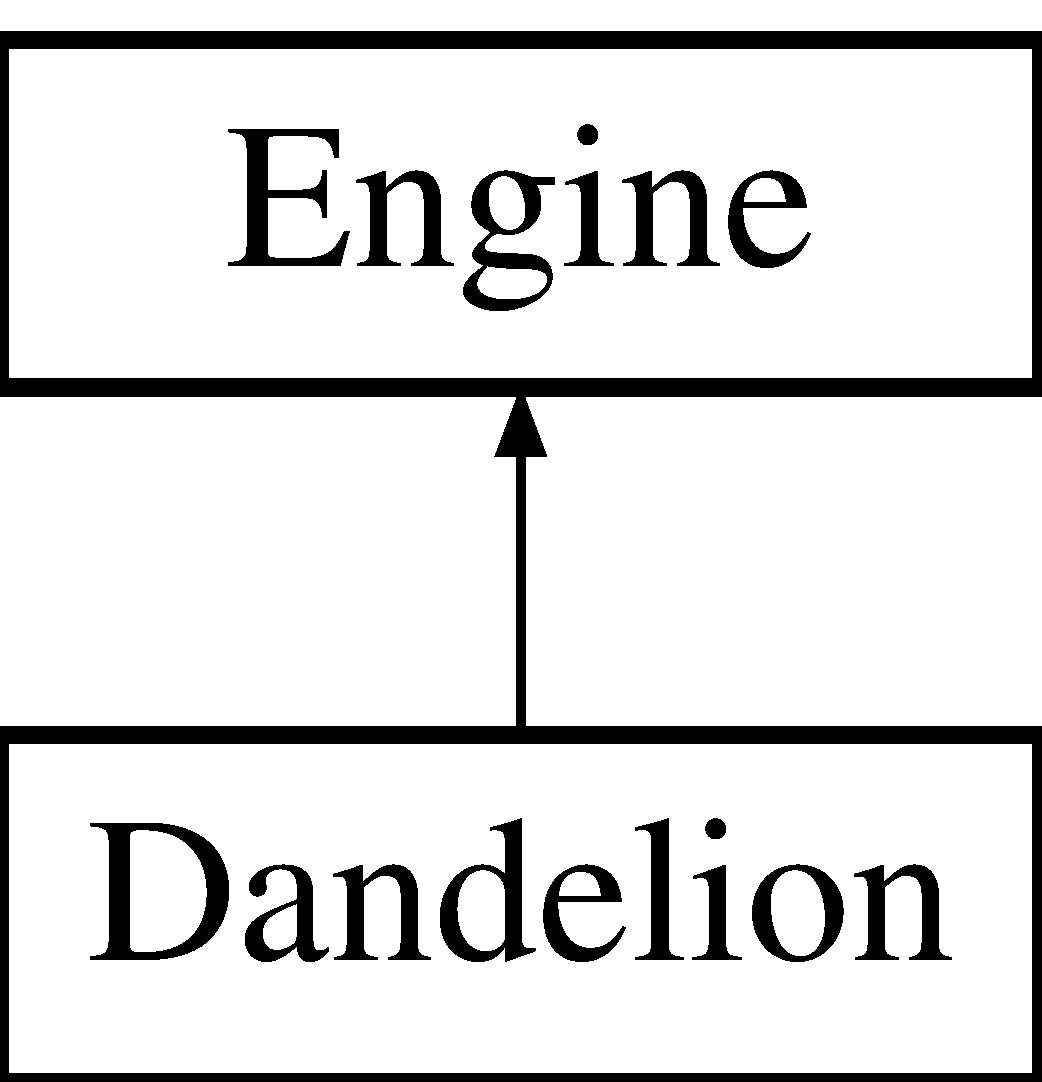
\includegraphics[height=2cm]{classDandelion}
\end{center}
\end{figure}
\subsection*{Public Member Functions}
\begin{DoxyCompactItemize}
\item 
\hyperlink{classDandelion_a8acd2b60d257ea45b85db1b0313c5fc2}{Dandelion} ()
\item 
\hyperlink{classDandelion_a94b7ff6276f9b31f3c1d25472480a062}{Dandelion} (\hyperlink{classDataAccess}{DataAccess} $\ast$)
\item 
\hyperlink{classDandelion_a48cd43f23ee97a671a5d5f55199545cb}{$\sim$Dandelion} ()
\item 
virtual void \hyperlink{classDandelion_a6c58019c7b1d8fb5a80c2031afb01374}{init} ()
\item 
virtual void \hyperlink{classDandelion_a21fa4068a4293d3c5068d53627e49393}{preProcess} ()
\item 
virtual void \hyperlink{classDandelion_a3de169eab0899f277a3747a57c94bb0b}{process} ()
\item 
virtual void \hyperlink{classDandelion_ac95a20aaaff8170c4539e047cb7a551a}{enslave} (\hyperlink{classEngineParamReader}{EngineParamReader} $\ast$)
\item 
virtual void \hyperlink{classDandelion_aad49aeddeaaf1aa98da869d94777e130}{test} ()
\end{DoxyCompactItemize}
\subsection*{Protected Member Functions}
\begin{DoxyCompactItemize}
\item 
void \hyperlink{classDandelion_adafc0b99e228f6bdfba301f129e17145}{delete\_\-my\_\-innards} ()
\item 
vector$<$ char $>$ \hyperlink{classDandelion_ac02d091e91f5ffc64665e1c986a843c4}{prepAlleles} (unsigned int row, int divisor, int beg, int end)
\item 
void \hyperlink{classDandelion_a7d005ed3065f6d59bcdb569ac60a80d1}{computeHaplotypeTest} (\hyperlink{structDandelionHaploInfo}{DandelionHaploInfo} \&d)
\item 
void \hyperlink{classDandelion_adf05e6be9d35362f836768eb1b7f22d8}{runSet} (int begin, int end)
\end{DoxyCompactItemize}
\subsection*{Static Protected Member Functions}
\begin{DoxyCompactItemize}
\item 
static double \hyperlink{classDandelion_a8679c05d30fc55999636726595c070ad}{EPS} ()
\end{DoxyCompactItemize}
\subsection*{Protected Attributes}
\begin{DoxyCompactItemize}
\item 
\hyperlink{classEngineParamReader}{EngineParamReader} $\ast$ \hyperlink{classDandelion_a6be9455eb19cec16f641f4b1e38dd12f}{ld\_\-param}
\item 
bool \hyperlink{classDandelion_a515b2e24d0761fb1278fc61818af02da}{haveOwner}
\item 
\hyperlink{classDandelionOutput}{DandelionOutput} \hyperlink{classDandelion_ae3ac17eb2241e0c91255789c941dde82}{output}
\item 
int \hyperlink{classDandelion_af9f4a50b7b9d5ec2876f87244f171fde}{numInitSNPs}
\item 
int \hyperlink{classDandelion_aa966dd7a7a67dd93522d912aacba581c}{numInitPhen}
\item 
int \hyperlink{classDandelion_a7cb5314914aee687a770cfa31af761f4}{numFinalPhen}
\item 
int \hyperlink{classDandelion_a1b502dbaf2cbdcaaaf375632840d562e}{numCase}
\end{DoxyCompactItemize}


\subsection{Constructor \& Destructor Documentation}
\hypertarget{classDandelion_a8acd2b60d257ea45b85db1b0313c5fc2}{
\index{Dandelion@{Dandelion}!Dandelion@{Dandelion}}
\index{Dandelion@{Dandelion}!Dandelion@{Dandelion}}
\subsubsection[{Dandelion}]{\setlength{\rightskip}{0pt plus 5cm}Dandelion::Dandelion ()\hspace{0.3cm}{\ttfamily  \mbox{[}explicit\mbox{]}}}}
\label{classDandelion_a8acd2b60d257ea45b85db1b0313c5fc2}
\hypertarget{classDandelion_a94b7ff6276f9b31f3c1d25472480a062}{
\index{Dandelion@{Dandelion}!Dandelion@{Dandelion}}
\index{Dandelion@{Dandelion}!Dandelion@{Dandelion}}
\subsubsection[{Dandelion}]{\setlength{\rightskip}{0pt plus 5cm}Dandelion::Dandelion ({\bf DataAccess} $\ast$)\hspace{0.3cm}{\ttfamily  \mbox{[}explicit\mbox{]}}}}
\label{classDandelion_a94b7ff6276f9b31f3c1d25472480a062}
\hypertarget{classDandelion_a48cd43f23ee97a671a5d5f55199545cb}{
\index{Dandelion@{Dandelion}!$\sim$Dandelion@{$\sim$Dandelion}}
\index{$\sim$Dandelion@{$\sim$Dandelion}!Dandelion@{Dandelion}}
\subsubsection[{$\sim$Dandelion}]{\setlength{\rightskip}{0pt plus 5cm}Dandelion::$\sim$Dandelion ()}}
\label{classDandelion_a48cd43f23ee97a671a5d5f55199545cb}


\subsection{Member Function Documentation}
\hypertarget{classDandelion_a7d005ed3065f6d59bcdb569ac60a80d1}{
\index{Dandelion@{Dandelion}!computeHaplotypeTest@{computeHaplotypeTest}}
\index{computeHaplotypeTest@{computeHaplotypeTest}!Dandelion@{Dandelion}}
\subsubsection[{computeHaplotypeTest}]{\setlength{\rightskip}{0pt plus 5cm}void Dandelion::computeHaplotypeTest ({\bf DandelionHaploInfo} \& {\em d})\hspace{0.3cm}{\ttfamily  \mbox{[}protected\mbox{]}}}}
\label{classDandelion_a7d005ed3065f6d59bcdb569ac60a80d1}
Compute the statistics for this haplotype.

\begin{Desc}
\item[\hyperlink{deprecated__deprecated000001}{Deprecated}]This is currently a simple chi2 test. Needs to be done with LR. This code is NOT tested and should never be included in production app.\end{Desc}
\hypertarget{classDandelion_adafc0b99e228f6bdfba301f129e17145}{
\index{Dandelion@{Dandelion}!delete\_\-my\_\-innards@{delete\_\-my\_\-innards}}
\index{delete\_\-my\_\-innards@{delete\_\-my\_\-innards}!Dandelion@{Dandelion}}
\subsubsection[{delete\_\-my\_\-innards}]{\setlength{\rightskip}{0pt plus 5cm}void Dandelion::delete\_\-my\_\-innards ()\hspace{0.3cm}{\ttfamily  \mbox{[}protected\mbox{]}}}}
\label{classDandelion_adafc0b99e228f6bdfba301f129e17145}
\hypertarget{classDandelion_ac95a20aaaff8170c4539e047cb7a551a}{
\index{Dandelion@{Dandelion}!enslave@{enslave}}
\index{enslave@{enslave}!Dandelion@{Dandelion}}
\subsubsection[{enslave}]{\setlength{\rightskip}{0pt plus 5cm}void Dandelion::enslave ({\bf EngineParamReader} $\ast$ {\em e})\hspace{0.3cm}{\ttfamily  \mbox{[}virtual\mbox{]}}}}
\label{classDandelion_ac95a20aaaff8170c4539e047cb7a551a}


Implements \hyperlink{classEngine_a023e094182312b1732fe53754c2fe5cb}{Engine}.

\hypertarget{classDandelion_a8679c05d30fc55999636726595c070ad}{
\index{Dandelion@{Dandelion}!EPS@{EPS}}
\index{EPS@{EPS}!Dandelion@{Dandelion}}
\subsubsection[{EPS}]{\setlength{\rightskip}{0pt plus 5cm}static double Dandelion::EPS ()\hspace{0.3cm}{\ttfamily  \mbox{[}inline, static, protected\mbox{]}}}}
\label{classDandelion_a8679c05d30fc55999636726595c070ad}
\hypertarget{classDandelion_a6c58019c7b1d8fb5a80c2031afb01374}{
\index{Dandelion@{Dandelion}!init@{init}}
\index{init@{init}!Dandelion@{Dandelion}}
\subsubsection[{init}]{\setlength{\rightskip}{0pt plus 5cm}void Dandelion::init ()\hspace{0.3cm}{\ttfamily  \mbox{[}virtual\mbox{]}}}}
\label{classDandelion_a6c58019c7b1d8fb5a80c2031afb01374}
Performs several functions, not all documented here.

Main tasks: get engine specific parameters and read and prep data.

Param checks: map file present (does not currently exit) 

Implements \hyperlink{classEngine_aaa054d596fb8ced6e3eb4bee208f8c3d}{Engine}.

\hypertarget{classDandelion_ac02d091e91f5ffc64665e1c986a843c4}{
\index{Dandelion@{Dandelion}!prepAlleles@{prepAlleles}}
\index{prepAlleles@{prepAlleles}!Dandelion@{Dandelion}}
\subsubsection[{prepAlleles}]{\setlength{\rightskip}{0pt plus 5cm}vector$<$ char $>$ Dandelion::prepAlleles (unsigned int {\em row}, \/  int {\em divisor}, \/  int {\em beg}, \/  int {\em end})\hspace{0.3cm}{\ttfamily  \mbox{[}protected\mbox{]}}}}
\label{classDandelion_ac02d091e91f5ffc64665e1c986a843c4}
Prep allele list by breaking number apart and pulling either major or minor allele.


\begin{DoxyParams}{Parameters}
\item[{\em row}]An integer that signifies a haplotype. \item[{\em divisor}]The coding for divisor. Default is 2, but some codings use something else. \end{DoxyParams}
\begin{DoxyReturn}{Returns}
vector$<$char$>$ List of haplotypes. 
\end{DoxyReturn}
\hypertarget{classDandelion_a21fa4068a4293d3c5068d53627e49393}{
\index{Dandelion@{Dandelion}!preProcess@{preProcess}}
\index{preProcess@{preProcess}!Dandelion@{Dandelion}}
\subsubsection[{preProcess}]{\setlength{\rightskip}{0pt plus 5cm}void Dandelion::preProcess ()\hspace{0.3cm}{\ttfamily  \mbox{[}virtual\mbox{]}}}}
\label{classDandelion_a21fa4068a4293d3c5068d53627e49393}


Implements \hyperlink{classEngine_aec7076b8979a13c96eceb362437dc68c}{Engine}.

\hypertarget{classDandelion_a3de169eab0899f277a3747a57c94bb0b}{
\index{Dandelion@{Dandelion}!process@{process}}
\index{process@{process}!Dandelion@{Dandelion}}
\subsubsection[{process}]{\setlength{\rightskip}{0pt plus 5cm}void Dandelion::process ()\hspace{0.3cm}{\ttfamily  \mbox{[}virtual\mbox{]}}}}
\label{classDandelion_a3de169eab0899f277a3747a57c94bb0b}
Compute \hyperlink{classDandelion}{Dandelion} throughout.

Two paths: 1) If window was set then multiple runs are required. 2) If not, then run the whole set. 

Implements \hyperlink{classEngine_a005f8e277c3dea16ea05803fba223db7}{Engine}.

\hypertarget{classDandelion_adf05e6be9d35362f836768eb1b7f22d8}{
\index{Dandelion@{Dandelion}!runSet@{runSet}}
\index{runSet@{runSet}!Dandelion@{Dandelion}}
\subsubsection[{runSet}]{\setlength{\rightskip}{0pt plus 5cm}void Dandelion::runSet (int {\em begin}, \/  int {\em end})\hspace{0.3cm}{\ttfamily  \mbox{[}protected\mbox{]}}}}
\label{classDandelion_adf05e6be9d35362f836768eb1b7f22d8}
Perform dandelion computation on a single set of SNPs. These should be in order in the data set, and should include both begin and end.


\begin{DoxyParams}{Parameters}
\item[{\em begin}]The first SNP to use. \item[{\em end}]The final SNP to use. All in between begin and end are used. \end{DoxyParams}
\hypertarget{classDandelion_aad49aeddeaaf1aa98da869d94777e130}{
\index{Dandelion@{Dandelion}!test@{test}}
\index{test@{test}!Dandelion@{Dandelion}}
\subsubsection[{test}]{\setlength{\rightskip}{0pt plus 5cm}void Dandelion::test ()\hspace{0.3cm}{\ttfamily  \mbox{[}virtual\mbox{]}}}}
\label{classDandelion_aad49aeddeaaf1aa98da869d94777e130}


Implements \hyperlink{classEngine_a2927c4a4263809453063ad482c6434a4}{Engine}.



\subsection{Field Documentation}
\hypertarget{classDandelion_a515b2e24d0761fb1278fc61818af02da}{
\index{Dandelion@{Dandelion}!haveOwner@{haveOwner}}
\index{haveOwner@{haveOwner}!Dandelion@{Dandelion}}
\subsubsection[{haveOwner}]{\setlength{\rightskip}{0pt plus 5cm}bool {\bf Dandelion::haveOwner}\hspace{0.3cm}{\ttfamily  \mbox{[}protected\mbox{]}}}}
\label{classDandelion_a515b2e24d0761fb1278fc61818af02da}
\hypertarget{classDandelion_a6be9455eb19cec16f641f4b1e38dd12f}{
\index{Dandelion@{Dandelion}!ld\_\-param@{ld\_\-param}}
\index{ld\_\-param@{ld\_\-param}!Dandelion@{Dandelion}}
\subsubsection[{ld\_\-param}]{\setlength{\rightskip}{0pt plus 5cm}{\bf EngineParamReader}$\ast$ {\bf Dandelion::ld\_\-param}\hspace{0.3cm}{\ttfamily  \mbox{[}protected\mbox{]}}}}
\label{classDandelion_a6be9455eb19cec16f641f4b1e38dd12f}
\hypertarget{classDandelion_a1b502dbaf2cbdcaaaf375632840d562e}{
\index{Dandelion@{Dandelion}!numCase@{numCase}}
\index{numCase@{numCase}!Dandelion@{Dandelion}}
\subsubsection[{numCase}]{\setlength{\rightskip}{0pt plus 5cm}int {\bf Dandelion::numCase}\hspace{0.3cm}{\ttfamily  \mbox{[}protected\mbox{]}}}}
\label{classDandelion_a1b502dbaf2cbdcaaaf375632840d562e}
\hypertarget{classDandelion_a7cb5314914aee687a770cfa31af761f4}{
\index{Dandelion@{Dandelion}!numFinalPhen@{numFinalPhen}}
\index{numFinalPhen@{numFinalPhen}!Dandelion@{Dandelion}}
\subsubsection[{numFinalPhen}]{\setlength{\rightskip}{0pt plus 5cm}int {\bf Dandelion::numFinalPhen}\hspace{0.3cm}{\ttfamily  \mbox{[}protected\mbox{]}}}}
\label{classDandelion_a7cb5314914aee687a770cfa31af761f4}
\hypertarget{classDandelion_aa966dd7a7a67dd93522d912aacba581c}{
\index{Dandelion@{Dandelion}!numInitPhen@{numInitPhen}}
\index{numInitPhen@{numInitPhen}!Dandelion@{Dandelion}}
\subsubsection[{numInitPhen}]{\setlength{\rightskip}{0pt plus 5cm}int {\bf Dandelion::numInitPhen}\hspace{0.3cm}{\ttfamily  \mbox{[}protected\mbox{]}}}}
\label{classDandelion_aa966dd7a7a67dd93522d912aacba581c}
\hypertarget{classDandelion_af9f4a50b7b9d5ec2876f87244f171fde}{
\index{Dandelion@{Dandelion}!numInitSNPs@{numInitSNPs}}
\index{numInitSNPs@{numInitSNPs}!Dandelion@{Dandelion}}
\subsubsection[{numInitSNPs}]{\setlength{\rightskip}{0pt plus 5cm}int {\bf Dandelion::numInitSNPs}\hspace{0.3cm}{\ttfamily  \mbox{[}protected\mbox{]}}}}
\label{classDandelion_af9f4a50b7b9d5ec2876f87244f171fde}
\hypertarget{classDandelion_ae3ac17eb2241e0c91255789c941dde82}{
\index{Dandelion@{Dandelion}!output@{output}}
\index{output@{output}!Dandelion@{Dandelion}}
\subsubsection[{output}]{\setlength{\rightskip}{0pt plus 5cm}{\bf DandelionOutput} {\bf Dandelion::output}\hspace{0.3cm}{\ttfamily  \mbox{[}protected\mbox{]}}}}
\label{classDandelion_ae3ac17eb2241e0c91255789c941dde82}


The documentation for this class was generated from the following files:\begin{DoxyCompactItemize}
\item 
engine/dandelion/\hyperlink{dandelion_8hh}{dandelion.hh}\item 
engine/dandelion/\hyperlink{dandelion_8cpp}{dandelion.cpp}\end{DoxyCompactItemize}

\hypertarget{structDandelionHaploInfo}{
\section{DandelionHaploInfo Struct Reference}
\label{structDandelionHaploInfo}\index{DandelionHaploInfo@{DandelionHaploInfo}}
}


{\ttfamily \#include $<$dandelion\_\-out.hh$>$}

\subsection*{Data Fields}
\begin{DoxyCompactItemize}
\item 
vector$<$ char $>$ \hyperlink{structDandelionHaploInfo_af54d760696f9e4e7f3acaba503b6558c}{alleles}
\item 
double \hyperlink{structDandelionHaploInfo_a015f6e666bc1e405cd536576269d13b8}{freqCs}
\item 
double \hyperlink{structDandelionHaploInfo_aa3f299599bd3849b31a4e3490a0babbb}{freqCn}
\item 
double \hyperlink{structDandelionHaploInfo_aa2d64bf0ece7cb0b33e97e3ef12a21e3}{freqCb}
\item 
double \hyperlink{structDandelionHaploInfo_a3121158a7720b61247ecbc6e13b4c389}{z}
\item 
double \hyperlink{structDandelionHaploInfo_a987c710ff44dec51b853659f5b5450f1}{p}
\item 
double \hyperlink{structDandelionHaploInfo_a1342df0d3256a2378be3f3512810bce4}{OR}
\item 
double \hyperlink{structDandelionHaploInfo_a797db41ac3fb4e6360ec3e20cafe5999}{UCI}
\item 
double \hyperlink{structDandelionHaploInfo_a816709cc46ab54a0a6afe7e5e48d9a22}{LCI}
\end{DoxyCompactItemize}


\subsection{Field Documentation}
\hypertarget{structDandelionHaploInfo_af54d760696f9e4e7f3acaba503b6558c}{
\index{DandelionHaploInfo@{DandelionHaploInfo}!alleles@{alleles}}
\index{alleles@{alleles}!DandelionHaploInfo@{DandelionHaploInfo}}
\subsubsection[{alleles}]{\setlength{\rightskip}{0pt plus 5cm}vector$<$char$>$ {\bf DandelionHaploInfo::alleles}}}
\label{structDandelionHaploInfo_af54d760696f9e4e7f3acaba503b6558c}
\hypertarget{structDandelionHaploInfo_aa2d64bf0ece7cb0b33e97e3ef12a21e3}{
\index{DandelionHaploInfo@{DandelionHaploInfo}!freqCb@{freqCb}}
\index{freqCb@{freqCb}!DandelionHaploInfo@{DandelionHaploInfo}}
\subsubsection[{freqCb}]{\setlength{\rightskip}{0pt plus 5cm}double {\bf DandelionHaploInfo::freqCb}}}
\label{structDandelionHaploInfo_aa2d64bf0ece7cb0b33e97e3ef12a21e3}
\hypertarget{structDandelionHaploInfo_aa3f299599bd3849b31a4e3490a0babbb}{
\index{DandelionHaploInfo@{DandelionHaploInfo}!freqCn@{freqCn}}
\index{freqCn@{freqCn}!DandelionHaploInfo@{DandelionHaploInfo}}
\subsubsection[{freqCn}]{\setlength{\rightskip}{0pt plus 5cm}double {\bf DandelionHaploInfo::freqCn}}}
\label{structDandelionHaploInfo_aa3f299599bd3849b31a4e3490a0babbb}
\hypertarget{structDandelionHaploInfo_a015f6e666bc1e405cd536576269d13b8}{
\index{DandelionHaploInfo@{DandelionHaploInfo}!freqCs@{freqCs}}
\index{freqCs@{freqCs}!DandelionHaploInfo@{DandelionHaploInfo}}
\subsubsection[{freqCs}]{\setlength{\rightskip}{0pt plus 5cm}double {\bf DandelionHaploInfo::freqCs}}}
\label{structDandelionHaploInfo_a015f6e666bc1e405cd536576269d13b8}
\hypertarget{structDandelionHaploInfo_a816709cc46ab54a0a6afe7e5e48d9a22}{
\index{DandelionHaploInfo@{DandelionHaploInfo}!LCI@{LCI}}
\index{LCI@{LCI}!DandelionHaploInfo@{DandelionHaploInfo}}
\subsubsection[{LCI}]{\setlength{\rightskip}{0pt plus 5cm}double {\bf DandelionHaploInfo::LCI}}}
\label{structDandelionHaploInfo_a816709cc46ab54a0a6afe7e5e48d9a22}
\hypertarget{structDandelionHaploInfo_a1342df0d3256a2378be3f3512810bce4}{
\index{DandelionHaploInfo@{DandelionHaploInfo}!OR@{OR}}
\index{OR@{OR}!DandelionHaploInfo@{DandelionHaploInfo}}
\subsubsection[{OR}]{\setlength{\rightskip}{0pt plus 5cm}double {\bf DandelionHaploInfo::OR}}}
\label{structDandelionHaploInfo_a1342df0d3256a2378be3f3512810bce4}
\hypertarget{structDandelionHaploInfo_a987c710ff44dec51b853659f5b5450f1}{
\index{DandelionHaploInfo@{DandelionHaploInfo}!p@{p}}
\index{p@{p}!DandelionHaploInfo@{DandelionHaploInfo}}
\subsubsection[{p}]{\setlength{\rightskip}{0pt plus 5cm}double {\bf DandelionHaploInfo::p}}}
\label{structDandelionHaploInfo_a987c710ff44dec51b853659f5b5450f1}
\hypertarget{structDandelionHaploInfo_a797db41ac3fb4e6360ec3e20cafe5999}{
\index{DandelionHaploInfo@{DandelionHaploInfo}!UCI@{UCI}}
\index{UCI@{UCI}!DandelionHaploInfo@{DandelionHaploInfo}}
\subsubsection[{UCI}]{\setlength{\rightskip}{0pt plus 5cm}double {\bf DandelionHaploInfo::UCI}}}
\label{structDandelionHaploInfo_a797db41ac3fb4e6360ec3e20cafe5999}
\hypertarget{structDandelionHaploInfo_a3121158a7720b61247ecbc6e13b4c389}{
\index{DandelionHaploInfo@{DandelionHaploInfo}!z@{z}}
\index{z@{z}!DandelionHaploInfo@{DandelionHaploInfo}}
\subsubsection[{z}]{\setlength{\rightskip}{0pt plus 5cm}double {\bf DandelionHaploInfo::z}}}
\label{structDandelionHaploInfo_a3121158a7720b61247ecbc6e13b4c389}


The documentation for this struct was generated from the following file:\begin{DoxyCompactItemize}
\item 
engine/output/\hyperlink{dandelion__out_8hh}{dandelion\_\-out.hh}\end{DoxyCompactItemize}

\hypertarget{classDandelionOutput}{
\section{DandelionOutput Class Reference}
\label{classDandelionOutput}\index{DandelionOutput@{DandelionOutput}}
}


{\ttfamily \#include $<$dandelion\_\-out.hh$>$}

\subsection*{Public Member Functions}
\begin{DoxyCompactItemize}
\item 
\hyperlink{classDandelionOutput_ae562a10e412aea6c27caf8316b31eb99}{DandelionOutput} ()
\item 
\hyperlink{classDandelionOutput_aaf9c5c50d9328fb09f4a982c001f659f}{$\sim$DandelionOutput} ()
\item 
bool \hyperlink{classDandelionOutput_a93338e6f99505f5d261edac17a7199e4}{init} (\hyperlink{classParamReader}{ParamReader} $\ast$, \hyperlink{classEngineParamReader}{EngineParamReader} $\ast$, int numSnps, string message)
\item 
void \hyperlink{classDandelionOutput_a3b4644ac035b093a86e6cf9e45bd2fc3}{writeHeadSet} (const vector$<$ \hyperlink{structDandelionSnpInfo}{DandelionSnpInfo} $>$ \&snps)
\item 
void \hyperlink{classDandelionOutput_aef3d333c031d511dabfff9235b04566d}{setMaxPersonId} (int)
\item 
void \hyperlink{classDandelionOutput_a4688c66f48f4db8c01248707e40ceef2}{close} ()
\end{DoxyCompactItemize}
\subsection*{Protected Member Functions}
\begin{DoxyCompactItemize}
\item 
void \hyperlink{classDandelionOutput_a86c08bdbc0bce02269f0237361cc9d7d}{writeLine} ()
\item 
void \hyperlink{classDandelionOutput_a97207aef1bd36b64aa00710072b2739d}{writeLine} (const \hyperlink{structDandelionHaploInfo}{DandelionHaploInfo} \&)
\item 
void \hyperlink{classDandelionOutput_a156a4bbb16c88aa885fc09e9a7f381c5}{writeStatisticsLine} (double pval, double chiSq, int DF)
\item 
void \hyperlink{classDandelionOutput_a9697f01201040850bafa5ee8b44c5fc5}{writePProbLine} (const \hyperlink{structDandelionPProbInfo}{DandelionPProbInfo} \&)
\item 
void \hyperlink{classDandelionOutput_acff40c7e6f90361aa9a96195039f6016}{writeHeader} (int)
\end{DoxyCompactItemize}
\subsection*{Protected Attributes}
\begin{DoxyCompactItemize}
\item 
\hyperlink{classOutput}{Output} \hyperlink{classDandelionOutput_a51a7cd7b94daf399744a2bd091dbc893}{outMain}
\item 
\hyperlink{classOutput}{Output} \hyperlink{classDandelionOutput_a4600b137430cebc7b8d5926d516584a5}{outPProb}
\item 
int \hyperlink{classDandelionOutput_a3e9b9fa7f56b76760797e6a5e9ca84c9}{personIdSpace}
\end{DoxyCompactItemize}
\subsection*{Friends}
\begin{DoxyCompactItemize}
\item 
class \hyperlink{classDandelionOutput_a3d9ee1085aff51099ffe0efd4b300c8f}{Dandelion}
\end{DoxyCompactItemize}


\subsection{Constructor \& Destructor Documentation}
\hypertarget{classDandelionOutput_ae562a10e412aea6c27caf8316b31eb99}{
\index{DandelionOutput@{DandelionOutput}!DandelionOutput@{DandelionOutput}}
\index{DandelionOutput@{DandelionOutput}!DandelionOutput@{DandelionOutput}}
\subsubsection[{DandelionOutput}]{\setlength{\rightskip}{0pt plus 5cm}DandelionOutput::DandelionOutput ()}}
\label{classDandelionOutput_ae562a10e412aea6c27caf8316b31eb99}
\hypertarget{classDandelionOutput_aaf9c5c50d9328fb09f4a982c001f659f}{
\index{DandelionOutput@{DandelionOutput}!$\sim$DandelionOutput@{$\sim$DandelionOutput}}
\index{$\sim$DandelionOutput@{$\sim$DandelionOutput}!DandelionOutput@{DandelionOutput}}
\subsubsection[{$\sim$DandelionOutput}]{\setlength{\rightskip}{0pt plus 5cm}DandelionOutput::$\sim$DandelionOutput ()}}
\label{classDandelionOutput_aaf9c5c50d9328fb09f4a982c001f659f}


\subsection{Member Function Documentation}
\hypertarget{classDandelionOutput_a4688c66f48f4db8c01248707e40ceef2}{
\index{DandelionOutput@{DandelionOutput}!close@{close}}
\index{close@{close}!DandelionOutput@{DandelionOutput}}
\subsubsection[{close}]{\setlength{\rightskip}{0pt plus 5cm}void DandelionOutput::close ()}}
\label{classDandelionOutput_a4688c66f48f4db8c01248707e40ceef2}
\hypertarget{classDandelionOutput_a93338e6f99505f5d261edac17a7199e4}{
\index{DandelionOutput@{DandelionOutput}!init@{init}}
\index{init@{init}!DandelionOutput@{DandelionOutput}}
\subsubsection[{init}]{\setlength{\rightskip}{0pt plus 5cm}bool DandelionOutput::init ({\bf ParamReader} $\ast$ {\em param}, \/  {\bf EngineParamReader} $\ast$ {\em engine\_\-param}, \/  int {\em numSnps}, \/  string {\em message})}}
\label{classDandelionOutput_a93338e6f99505f5d261edac17a7199e4}
\hypertarget{classDandelionOutput_aef3d333c031d511dabfff9235b04566d}{
\index{DandelionOutput@{DandelionOutput}!setMaxPersonId@{setMaxPersonId}}
\index{setMaxPersonId@{setMaxPersonId}!DandelionOutput@{DandelionOutput}}
\subsubsection[{setMaxPersonId}]{\setlength{\rightskip}{0pt plus 5cm}void DandelionOutput::setMaxPersonId (int {\em maxPersonSize})}}
\label{classDandelionOutput_aef3d333c031d511dabfff9235b04566d}
Set personID.


\begin{DoxyParams}{Parameters}
\item[{\em int}]Size of person Id length. \end{DoxyParams}
\hypertarget{classDandelionOutput_acff40c7e6f90361aa9a96195039f6016}{
\index{DandelionOutput@{DandelionOutput}!writeHeader@{writeHeader}}
\index{writeHeader@{writeHeader}!DandelionOutput@{DandelionOutput}}
\subsubsection[{writeHeader}]{\setlength{\rightskip}{0pt plus 5cm}void DandelionOutput::writeHeader (int {\em numSnps})\hspace{0.3cm}{\ttfamily  \mbox{[}protected\mbox{]}}}}
\label{classDandelionOutput_acff40c7e6f90361aa9a96195039f6016}
\hypertarget{classDandelionOutput_a3b4644ac035b093a86e6cf9e45bd2fc3}{
\index{DandelionOutput@{DandelionOutput}!writeHeadSet@{writeHeadSet}}
\index{writeHeadSet@{writeHeadSet}!DandelionOutput@{DandelionOutput}}
\subsubsection[{writeHeadSet}]{\setlength{\rightskip}{0pt plus 5cm}void DandelionOutput::writeHeadSet (const vector$<$ {\bf DandelionSnpInfo} $>$ \& {\em snps})}}
\label{classDandelionOutput_a3b4644ac035b093a86e6cf9e45bd2fc3}
Write a header for a single series.


\begin{DoxyParams}{Parameters}
\item[{\em vector$<$DandelionSnpInfo$>$}]Set of SNPs.\end{DoxyParams}
Should look like:

Set of $<$num$>$ SNPs rs123 ma mi chr pos .... \hypertarget{classDandelionOutput_a97207aef1bd36b64aa00710072b2739d}{
\index{DandelionOutput@{DandelionOutput}!writeLine@{writeLine}}
\index{writeLine@{writeLine}!DandelionOutput@{DandelionOutput}}
\subsubsection[{writeLine}]{\setlength{\rightskip}{0pt plus 5cm}void DandelionOutput::writeLine (const {\bf DandelionHaploInfo} \& {\em d})\hspace{0.3cm}{\ttfamily  \mbox{[}protected\mbox{]}}}}
\label{classDandelionOutput_a97207aef1bd36b64aa00710072b2739d}
\hypertarget{classDandelionOutput_a86c08bdbc0bce02269f0237361cc9d7d}{
\index{DandelionOutput@{DandelionOutput}!writeLine@{writeLine}}
\index{writeLine@{writeLine}!DandelionOutput@{DandelionOutput}}
\subsubsection[{writeLine}]{\setlength{\rightskip}{0pt plus 5cm}void DandelionOutput::writeLine ()\hspace{0.3cm}{\ttfamily  \mbox{[}protected\mbox{]}}}}
\label{classDandelionOutput_a86c08bdbc0bce02269f0237361cc9d7d}
\hypertarget{classDandelionOutput_a9697f01201040850bafa5ee8b44c5fc5}{
\index{DandelionOutput@{DandelionOutput}!writePProbLine@{writePProbLine}}
\index{writePProbLine@{writePProbLine}!DandelionOutput@{DandelionOutput}}
\subsubsection[{writePProbLine}]{\setlength{\rightskip}{0pt plus 5cm}void DandelionOutput::writePProbLine (const {\bf DandelionPProbInfo} \& {\em p})\hspace{0.3cm}{\ttfamily  \mbox{[}protected\mbox{]}}}}
\label{classDandelionOutput_a9697f01201040850bafa5ee8b44c5fc5}
Write a line of output to the pprob file.


\begin{DoxyParams}{Parameters}
\item[{\em \hyperlink{structDandelionPProbInfo}{DandelionPProbInfo}}]Holds the information to be written. \end{DoxyParams}
\hypertarget{classDandelionOutput_a156a4bbb16c88aa885fc09e9a7f381c5}{
\index{DandelionOutput@{DandelionOutput}!writeStatisticsLine@{writeStatisticsLine}}
\index{writeStatisticsLine@{writeStatisticsLine}!DandelionOutput@{DandelionOutput}}
\subsubsection[{writeStatisticsLine}]{\setlength{\rightskip}{0pt plus 5cm}void DandelionOutput::writeStatisticsLine (double {\em pval}, \/  double {\em chiSq}, \/  int {\em DF})\hspace{0.3cm}{\ttfamily  \mbox{[}protected\mbox{]}}}}
\label{classDandelionOutput_a156a4bbb16c88aa885fc09e9a7f381c5}


\subsection{Friends And Related Function Documentation}
\hypertarget{classDandelionOutput_a3d9ee1085aff51099ffe0efd4b300c8f}{
\index{DandelionOutput@{DandelionOutput}!Dandelion@{Dandelion}}
\index{Dandelion@{Dandelion}!DandelionOutput@{DandelionOutput}}
\subsubsection[{Dandelion}]{\setlength{\rightskip}{0pt plus 5cm}friend class {\bf Dandelion}\hspace{0.3cm}{\ttfamily  \mbox{[}friend\mbox{]}}}}
\label{classDandelionOutput_a3d9ee1085aff51099ffe0efd4b300c8f}


\subsection{Field Documentation}
\hypertarget{classDandelionOutput_a51a7cd7b94daf399744a2bd091dbc893}{
\index{DandelionOutput@{DandelionOutput}!outMain@{outMain}}
\index{outMain@{outMain}!DandelionOutput@{DandelionOutput}}
\subsubsection[{outMain}]{\setlength{\rightskip}{0pt plus 5cm}{\bf Output} {\bf DandelionOutput::outMain}\hspace{0.3cm}{\ttfamily  \mbox{[}protected\mbox{]}}}}
\label{classDandelionOutput_a51a7cd7b94daf399744a2bd091dbc893}
\hypertarget{classDandelionOutput_a4600b137430cebc7b8d5926d516584a5}{
\index{DandelionOutput@{DandelionOutput}!outPProb@{outPProb}}
\index{outPProb@{outPProb}!DandelionOutput@{DandelionOutput}}
\subsubsection[{outPProb}]{\setlength{\rightskip}{0pt plus 5cm}{\bf Output} {\bf DandelionOutput::outPProb}\hspace{0.3cm}{\ttfamily  \mbox{[}protected\mbox{]}}}}
\label{classDandelionOutput_a4600b137430cebc7b8d5926d516584a5}
\hypertarget{classDandelionOutput_a3e9b9fa7f56b76760797e6a5e9ca84c9}{
\index{DandelionOutput@{DandelionOutput}!personIdSpace@{personIdSpace}}
\index{personIdSpace@{personIdSpace}!DandelionOutput@{DandelionOutput}}
\subsubsection[{personIdSpace}]{\setlength{\rightskip}{0pt plus 5cm}int {\bf DandelionOutput::personIdSpace}\hspace{0.3cm}{\ttfamily  \mbox{[}protected\mbox{]}}}}
\label{classDandelionOutput_a3e9b9fa7f56b76760797e6a5e9ca84c9}


The documentation for this class was generated from the following files:\begin{DoxyCompactItemize}
\item 
engine/output/\hyperlink{dandelion__out_8hh}{dandelion\_\-out.hh}\item 
engine/output/\hyperlink{dandelion__out_8cpp}{dandelion\_\-out.cpp}\end{DoxyCompactItemize}

\hypertarget{structDandelionPProbInfo}{
\section{DandelionPProbInfo Struct Reference}
\label{structDandelionPProbInfo}\index{DandelionPProbInfo@{DandelionPProbInfo}}
}


{\ttfamily \#include $<$dandelion\_\-out.hh$>$}

\subsection*{Data Fields}
\begin{DoxyCompactItemize}
\item 
int \hyperlink{structDandelionPProbInfo_a4acbb51690c01dfaa81827a2ef8ae5ad}{personNum}
\item 
double \hyperlink{structDandelionPProbInfo_aa0be0c72636bfa42d72322b0f16bd3a0}{affectionStatus}
\item 
vector$<$ char $>$ \hyperlink{structDandelionPProbInfo_a7613ee43c9ecc04d4443e4df209b9577}{leftHap}
\item 
vector$<$ char $>$ \hyperlink{structDandelionPProbInfo_a015d844a48d0b96a19684df86b0bf959}{rightHap}
\item 
double \hyperlink{structDandelionPProbInfo_ac4034ca65eee810a5f0267baa47f1420}{prob}
\item 
string \hyperlink{structDandelionPProbInfo_a19a65f30f8d4ee9272191119b35724f5}{personID}
\end{DoxyCompactItemize}


\subsection{Field Documentation}
\hypertarget{structDandelionPProbInfo_aa0be0c72636bfa42d72322b0f16bd3a0}{
\index{DandelionPProbInfo@{DandelionPProbInfo}!affectionStatus@{affectionStatus}}
\index{affectionStatus@{affectionStatus}!DandelionPProbInfo@{DandelionPProbInfo}}
\subsubsection[{affectionStatus}]{\setlength{\rightskip}{0pt plus 5cm}double {\bf DandelionPProbInfo::affectionStatus}}}
\label{structDandelionPProbInfo_aa0be0c72636bfa42d72322b0f16bd3a0}
\hypertarget{structDandelionPProbInfo_a7613ee43c9ecc04d4443e4df209b9577}{
\index{DandelionPProbInfo@{DandelionPProbInfo}!leftHap@{leftHap}}
\index{leftHap@{leftHap}!DandelionPProbInfo@{DandelionPProbInfo}}
\subsubsection[{leftHap}]{\setlength{\rightskip}{0pt plus 5cm}vector$<$char$>$ {\bf DandelionPProbInfo::leftHap}}}
\label{structDandelionPProbInfo_a7613ee43c9ecc04d4443e4df209b9577}
\hypertarget{structDandelionPProbInfo_a19a65f30f8d4ee9272191119b35724f5}{
\index{DandelionPProbInfo@{DandelionPProbInfo}!personID@{personID}}
\index{personID@{personID}!DandelionPProbInfo@{DandelionPProbInfo}}
\subsubsection[{personID}]{\setlength{\rightskip}{0pt plus 5cm}string {\bf DandelionPProbInfo::personID}}}
\label{structDandelionPProbInfo_a19a65f30f8d4ee9272191119b35724f5}
\hypertarget{structDandelionPProbInfo_a4acbb51690c01dfaa81827a2ef8ae5ad}{
\index{DandelionPProbInfo@{DandelionPProbInfo}!personNum@{personNum}}
\index{personNum@{personNum}!DandelionPProbInfo@{DandelionPProbInfo}}
\subsubsection[{personNum}]{\setlength{\rightskip}{0pt plus 5cm}int {\bf DandelionPProbInfo::personNum}}}
\label{structDandelionPProbInfo_a4acbb51690c01dfaa81827a2ef8ae5ad}
\hypertarget{structDandelionPProbInfo_ac4034ca65eee810a5f0267baa47f1420}{
\index{DandelionPProbInfo@{DandelionPProbInfo}!prob@{prob}}
\index{prob@{prob}!DandelionPProbInfo@{DandelionPProbInfo}}
\subsubsection[{prob}]{\setlength{\rightskip}{0pt plus 5cm}double {\bf DandelionPProbInfo::prob}}}
\label{structDandelionPProbInfo_ac4034ca65eee810a5f0267baa47f1420}
\hypertarget{structDandelionPProbInfo_a015d844a48d0b96a19684df86b0bf959}{
\index{DandelionPProbInfo@{DandelionPProbInfo}!rightHap@{rightHap}}
\index{rightHap@{rightHap}!DandelionPProbInfo@{DandelionPProbInfo}}
\subsubsection[{rightHap}]{\setlength{\rightskip}{0pt plus 5cm}vector$<$char$>$ {\bf DandelionPProbInfo::rightHap}}}
\label{structDandelionPProbInfo_a015d844a48d0b96a19684df86b0bf959}


The documentation for this struct was generated from the following file:\begin{DoxyCompactItemize}
\item 
engine/output/\hyperlink{dandelion__out_8hh}{dandelion\_\-out.hh}\end{DoxyCompactItemize}

\hypertarget{structDandelionSnpInfo}{
\section{DandelionSnpInfo Struct Reference}
\label{structDandelionSnpInfo}\index{DandelionSnpInfo@{DandelionSnpInfo}}
}


{\ttfamily \#include $<$dandelion\_\-out.hh$>$}

\subsection*{Data Fields}
\begin{DoxyCompactItemize}
\item 
int \hyperlink{structDandelionSnpInfo_a1fa282f1f892a1b5fd1223ce17e203cb}{index}
\item 
string \hyperlink{structDandelionSnpInfo_aaf39c2953bf283cb8684110114aee7b7}{name}
\item 
string \hyperlink{structDandelionSnpInfo_a8bb8f2cdf3f4261e9f3d8bc04c8940c0}{chr}
\item 
int \hyperlink{structDandelionSnpInfo_a4aaf965cd75aaca6d80a14b2e9a3e0be}{position}
\item 
char \hyperlink{structDandelionSnpInfo_a1657e9bf3a6583c4aa5bf892731a42be}{majAllele}
\item 
char \hyperlink{structDandelionSnpInfo_ae6f55705afbd04f010f075229878c7fc}{minAllele}
\item 
char \hyperlink{structDandelionSnpInfo_a9d8144ecc88436ada470a03fe77bb487}{refAllele}
\end{DoxyCompactItemize}


\subsection{Field Documentation}
\hypertarget{structDandelionSnpInfo_a8bb8f2cdf3f4261e9f3d8bc04c8940c0}{
\index{DandelionSnpInfo@{DandelionSnpInfo}!chr@{chr}}
\index{chr@{chr}!DandelionSnpInfo@{DandelionSnpInfo}}
\subsubsection[{chr}]{\setlength{\rightskip}{0pt plus 5cm}string {\bf DandelionSnpInfo::chr}}}
\label{structDandelionSnpInfo_a8bb8f2cdf3f4261e9f3d8bc04c8940c0}
\hypertarget{structDandelionSnpInfo_a1fa282f1f892a1b5fd1223ce17e203cb}{
\index{DandelionSnpInfo@{DandelionSnpInfo}!index@{index}}
\index{index@{index}!DandelionSnpInfo@{DandelionSnpInfo}}
\subsubsection[{index}]{\setlength{\rightskip}{0pt plus 5cm}int {\bf DandelionSnpInfo::index}}}
\label{structDandelionSnpInfo_a1fa282f1f892a1b5fd1223ce17e203cb}
\hypertarget{structDandelionSnpInfo_a1657e9bf3a6583c4aa5bf892731a42be}{
\index{DandelionSnpInfo@{DandelionSnpInfo}!majAllele@{majAllele}}
\index{majAllele@{majAllele}!DandelionSnpInfo@{DandelionSnpInfo}}
\subsubsection[{majAllele}]{\setlength{\rightskip}{0pt plus 5cm}char {\bf DandelionSnpInfo::majAllele}}}
\label{structDandelionSnpInfo_a1657e9bf3a6583c4aa5bf892731a42be}
\hypertarget{structDandelionSnpInfo_ae6f55705afbd04f010f075229878c7fc}{
\index{DandelionSnpInfo@{DandelionSnpInfo}!minAllele@{minAllele}}
\index{minAllele@{minAllele}!DandelionSnpInfo@{DandelionSnpInfo}}
\subsubsection[{minAllele}]{\setlength{\rightskip}{0pt plus 5cm}char {\bf DandelionSnpInfo::minAllele}}}
\label{structDandelionSnpInfo_ae6f55705afbd04f010f075229878c7fc}
\hypertarget{structDandelionSnpInfo_aaf39c2953bf283cb8684110114aee7b7}{
\index{DandelionSnpInfo@{DandelionSnpInfo}!name@{name}}
\index{name@{name}!DandelionSnpInfo@{DandelionSnpInfo}}
\subsubsection[{name}]{\setlength{\rightskip}{0pt plus 5cm}string {\bf DandelionSnpInfo::name}}}
\label{structDandelionSnpInfo_aaf39c2953bf283cb8684110114aee7b7}
\hypertarget{structDandelionSnpInfo_a4aaf965cd75aaca6d80a14b2e9a3e0be}{
\index{DandelionSnpInfo@{DandelionSnpInfo}!position@{position}}
\index{position@{position}!DandelionSnpInfo@{DandelionSnpInfo}}
\subsubsection[{position}]{\setlength{\rightskip}{0pt plus 5cm}int {\bf DandelionSnpInfo::position}}}
\label{structDandelionSnpInfo_a4aaf965cd75aaca6d80a14b2e9a3e0be}
\hypertarget{structDandelionSnpInfo_a9d8144ecc88436ada470a03fe77bb487}{
\index{DandelionSnpInfo@{DandelionSnpInfo}!refAllele@{refAllele}}
\index{refAllele@{refAllele}!DandelionSnpInfo@{DandelionSnpInfo}}
\subsubsection[{refAllele}]{\setlength{\rightskip}{0pt plus 5cm}char {\bf DandelionSnpInfo::refAllele}}}
\label{structDandelionSnpInfo_a9d8144ecc88436ada470a03fe77bb487}


The documentation for this struct was generated from the following file:\begin{DoxyCompactItemize}
\item 
engine/output/\hyperlink{dandelion__out_8hh}{dandelion\_\-out.hh}\end{DoxyCompactItemize}

\hypertarget{classDataAccess}{
\section{DataAccess Class Reference}
\label{classDataAccess}\index{DataAccess@{DataAccess}}
}


{\ttfamily \#include $<$data\_\-plugin.h$>$}

\subsection*{Public Member Functions}
\begin{DoxyCompactItemize}
\item 
\hyperlink{classDataAccess_af99b77ec290d1e723d0540ba9d9a95ba}{DataAccess} ()
\item 
void \hyperlink{classDataAccess_a2a55acc88408a8b40f49e4a5330e2113}{init} (\hyperlink{classSnpData}{SnpData} $\ast$)
\item 
\hyperlink{classDataAccess_a02d65c4dff5b263dddb2d90d695fbe0e}{$\sim$DataAccess} ()
\item 
void \hyperlink{classDataAccess_a4d138b5b230fa651f3f9d7ac31ebcbc4}{setRedirectBootstrap} ()
\item 
vector$<$ short $>$ $\ast$ \hyperlink{classDataAccess_a8085d15c2180ac572bc39e937171a256}{get\_\-data} (int)
\item 
double \hyperlink{classDataAccess_a52b91927560b4221d1095d7bb0dea4b1}{get\_\-phenotype} (int)
\item 
int \hyperlink{classDataAccess_a0c3ef8b90d5b9547d9084b93f2866732}{pheno\_\-size} ()
\item 
int \hyperlink{classDataAccess_a50b8be12574c5c4f454a0bbde76e0ea2}{geno\_\-size} ()
\item 
vector$<$ double $>$ $\ast$ \hyperlink{classDataAccess_aa4ffa6d4d9cf70fb34a3ab1d8227e895}{get\_\-covariates} (int)
\item 
string \hyperlink{classDataAccess_a323b6639c751a4512cc83577715b0e80}{get\_\-chrom} (int)
\item 
void \hyperlink{classDataAccess_ac4f80d59b3ff2178f456f7907bb2479a}{get\_\-map\_\-info} (int, string \&chr, string \&name, int \&position)
\item 
void \hyperlink{classDataAccess_a7476ba5cf613f7172cc1386895c637b8}{get\_\-allele\_\-codes} (int, char \&maj, char \&min, char \&ref)
\item 
int \hyperlink{classDataAccess_a8a0848d14c6c294abdee288348a02b75}{max\_\-map\_\-size} ()
\item 
string \hyperlink{classDataAccess_ae446b940e538a5d09f651c4908e08804}{get\_\-person\_\-ID} (int)
\item 
string \hyperlink{classDataAccess_ad58bd17d7e8f99412d453570b2ac3be8}{snp\_\-name} (long l)
\item 
long \hyperlink{classDataAccess_a97e83c12c8798f13bedcacdcc6e75178}{snp\_\-size} (unsigned int o)
\item 
int \hyperlink{classDataAccess_a5ff27046517657f20a3672d946e0fb47}{max\_\-person\_\-ID\_\-size} ()
\item 
void \hyperlink{classDataAccess_a3f3a33a79e44ba86fa1516e965a7348c}{make\_\-categorical} (int low, int hi)
\item 
\hyperlink{classSnpData}{SnpData} $\ast$ \hyperlink{classDataAccess_adcb83e7fdf831ae7b22902ccec055daa}{getDataObject} ()
\end{DoxyCompactItemize}
\subsection*{Protected Attributes}
\begin{DoxyCompactItemize}
\item 
\hyperlink{classSnpData}{SnpData} $\ast$ \hyperlink{classDataAccess_a37987750a9f946993ddad2245a8c5c54}{data}
\item 
vector$<$ unsigned int $>$ \hyperlink{classDataAccess_a642900c2d22f2b850213d46fe819206c}{redirect}
\item 
bool \hyperlink{classDataAccess_ac49207f016cee4af4c245c8c7fd5fb60}{uses\_\-redirect}
\item 
bool \hyperlink{classDataAccess_a227068cc74d5c6d3f001d32ebf24a06e}{owns\_\-data}
\end{DoxyCompactItemize}


\subsection{Constructor \& Destructor Documentation}
\hypertarget{classDataAccess_af99b77ec290d1e723d0540ba9d9a95ba}{
\index{DataAccess@{DataAccess}!DataAccess@{DataAccess}}
\index{DataAccess@{DataAccess}!DataAccess@{DataAccess}}
\subsubsection[{DataAccess}]{\setlength{\rightskip}{0pt plus 5cm}DataAccess::DataAccess ()}}
\label{classDataAccess_af99b77ec290d1e723d0540ba9d9a95ba}
\hypertarget{classDataAccess_a02d65c4dff5b263dddb2d90d695fbe0e}{
\index{DataAccess@{DataAccess}!$\sim$DataAccess@{$\sim$DataAccess}}
\index{$\sim$DataAccess@{$\sim$DataAccess}!DataAccess@{DataAccess}}
\subsubsection[{$\sim$DataAccess}]{\setlength{\rightskip}{0pt plus 5cm}DataAccess::$\sim$DataAccess ()}}
\label{classDataAccess_a02d65c4dff5b263dddb2d90d695fbe0e}


\subsection{Member Function Documentation}
\hypertarget{classDataAccess_a50b8be12574c5c4f454a0bbde76e0ea2}{
\index{DataAccess@{DataAccess}!geno\_\-size@{geno\_\-size}}
\index{geno\_\-size@{geno\_\-size}!DataAccess@{DataAccess}}
\subsubsection[{geno\_\-size}]{\setlength{\rightskip}{0pt plus 5cm}int DataAccess::geno\_\-size ()}}
\label{classDataAccess_a50b8be12574c5c4f454a0bbde76e0ea2}
Return number of SNPs in the data set

\begin{DoxyReturn}{Returns}
int Number of SNPs. 
\end{DoxyReturn}
\hypertarget{classDataAccess_a7476ba5cf613f7172cc1386895c637b8}{
\index{DataAccess@{DataAccess}!get\_\-allele\_\-codes@{get\_\-allele\_\-codes}}
\index{get\_\-allele\_\-codes@{get\_\-allele\_\-codes}!DataAccess@{DataAccess}}
\subsubsection[{get\_\-allele\_\-codes}]{\setlength{\rightskip}{0pt plus 5cm}void DataAccess::get\_\-allele\_\-codes (int {\em i}, \/  char \& {\em maj}, \/  char \& {\em min}, \/  char \& {\em ref})}}
\label{classDataAccess_a7476ba5cf613f7172cc1386895c637b8}
\hypertarget{classDataAccess_a323b6639c751a4512cc83577715b0e80}{
\index{DataAccess@{DataAccess}!get\_\-chrom@{get\_\-chrom}}
\index{get\_\-chrom@{get\_\-chrom}!DataAccess@{DataAccess}}
\subsubsection[{get\_\-chrom}]{\setlength{\rightskip}{0pt plus 5cm}string DataAccess::get\_\-chrom (int {\em i})}}
\label{classDataAccess_a323b6639c751a4512cc83577715b0e80}
\hypertarget{classDataAccess_aa4ffa6d4d9cf70fb34a3ab1d8227e895}{
\index{DataAccess@{DataAccess}!get\_\-covariates@{get\_\-covariates}}
\index{get\_\-covariates@{get\_\-covariates}!DataAccess@{DataAccess}}
\subsubsection[{get\_\-covariates}]{\setlength{\rightskip}{0pt plus 5cm}vector$<$ double $>$ $\ast$ DataAccess::get\_\-covariates (int {\em i})}}
\label{classDataAccess_aa4ffa6d4d9cf70fb34a3ab1d8227e895}
\hypertarget{classDataAccess_a8085d15c2180ac572bc39e937171a256}{
\index{DataAccess@{DataAccess}!get\_\-data@{get\_\-data}}
\index{get\_\-data@{get\_\-data}!DataAccess@{DataAccess}}
\subsubsection[{get\_\-data}]{\setlength{\rightskip}{0pt plus 5cm}vector$<$ short $>$ $\ast$ DataAccess::get\_\-data (int {\em i})}}
\label{classDataAccess_a8085d15c2180ac572bc39e937171a256}
Return all SNPs for a single individual in form of a pointer. If this \hyperlink{classDataAccess}{DataAccess} object uses redirection, then the method figures out which individual to actually return.


\begin{DoxyParams}{Parameters}
\item[{\em i}]The individual whose data is returned \end{DoxyParams}
\begin{DoxyReturn}{Returns}
vector$<$short$>$ $\ast$ A pointer to the vector of data for the individual queried. 
\end{DoxyReturn}
\hypertarget{classDataAccess_ac4f80d59b3ff2178f456f7907bb2479a}{
\index{DataAccess@{DataAccess}!get\_\-map\_\-info@{get\_\-map\_\-info}}
\index{get\_\-map\_\-info@{get\_\-map\_\-info}!DataAccess@{DataAccess}}
\subsubsection[{get\_\-map\_\-info}]{\setlength{\rightskip}{0pt plus 5cm}void DataAccess::get\_\-map\_\-info (int {\em i}, \/  string \& {\em chr}, \/  string \& {\em name}, \/  int \& {\em position})}}
\label{classDataAccess_ac4f80d59b3ff2178f456f7907bb2479a}
\hypertarget{classDataAccess_ae446b940e538a5d09f651c4908e08804}{
\index{DataAccess@{DataAccess}!get\_\-person\_\-ID@{get\_\-person\_\-ID}}
\index{get\_\-person\_\-ID@{get\_\-person\_\-ID}!DataAccess@{DataAccess}}
\subsubsection[{get\_\-person\_\-ID}]{\setlength{\rightskip}{0pt plus 5cm}string DataAccess::get\_\-person\_\-ID (int {\em i})}}
\label{classDataAccess_ae446b940e538a5d09f651c4908e08804}
Return a person ID 
\begin{DoxyParams}{Parameters}
\item[{\em int}]the person index. \end{DoxyParams}
\hypertarget{classDataAccess_a52b91927560b4221d1095d7bb0dea4b1}{
\index{DataAccess@{DataAccess}!get\_\-phenotype@{get\_\-phenotype}}
\index{get\_\-phenotype@{get\_\-phenotype}!DataAccess@{DataAccess}}
\subsubsection[{get\_\-phenotype}]{\setlength{\rightskip}{0pt plus 5cm}double DataAccess::get\_\-phenotype (int {\em i})}}
\label{classDataAccess_a52b91927560b4221d1095d7bb0dea4b1}
\hypertarget{classDataAccess_adcb83e7fdf831ae7b22902ccec055daa}{
\index{DataAccess@{DataAccess}!getDataObject@{getDataObject}}
\index{getDataObject@{getDataObject}!DataAccess@{DataAccess}}
\subsubsection[{getDataObject}]{\setlength{\rightskip}{0pt plus 5cm}{\bf SnpData}$\ast$ DataAccess::getDataObject ()\hspace{0.3cm}{\ttfamily  \mbox{[}inline\mbox{]}}}}
\label{classDataAccess_adcb83e7fdf831ae7b22902ccec055daa}
\hypertarget{classDataAccess_a2a55acc88408a8b40f49e4a5330e2113}{
\index{DataAccess@{DataAccess}!init@{init}}
\index{init@{init}!DataAccess@{DataAccess}}
\subsubsection[{init}]{\setlength{\rightskip}{0pt plus 5cm}void DataAccess::init ({\bf SnpData} $\ast$ {\em d})}}
\label{classDataAccess_a2a55acc88408a8b40f49e4a5330e2113}
\hypertarget{classDataAccess_a3f3a33a79e44ba86fa1516e965a7348c}{
\index{DataAccess@{DataAccess}!make\_\-categorical@{make\_\-categorical}}
\index{make\_\-categorical@{make\_\-categorical}!DataAccess@{DataAccess}}
\subsubsection[{make\_\-categorical}]{\setlength{\rightskip}{0pt plus 5cm}void DataAccess::make\_\-categorical (int {\em low}, \/  int {\em hi})}}
\label{classDataAccess_a3f3a33a79e44ba86fa1516e965a7348c}
\hypertarget{classDataAccess_a8a0848d14c6c294abdee288348a02b75}{
\index{DataAccess@{DataAccess}!max\_\-map\_\-size@{max\_\-map\_\-size}}
\index{max\_\-map\_\-size@{max\_\-map\_\-size}!DataAccess@{DataAccess}}
\subsubsection[{max\_\-map\_\-size}]{\setlength{\rightskip}{0pt plus 5cm}int DataAccess::max\_\-map\_\-size ()}}
\label{classDataAccess_a8a0848d14c6c294abdee288348a02b75}
\hypertarget{classDataAccess_a5ff27046517657f20a3672d946e0fb47}{
\index{DataAccess@{DataAccess}!max\_\-person\_\-ID\_\-size@{max\_\-person\_\-ID\_\-size}}
\index{max\_\-person\_\-ID\_\-size@{max\_\-person\_\-ID\_\-size}!DataAccess@{DataAccess}}
\subsubsection[{max\_\-person\_\-ID\_\-size}]{\setlength{\rightskip}{0pt plus 5cm}int DataAccess::max\_\-person\_\-ID\_\-size ()\hspace{0.3cm}{\ttfamily  \mbox{[}inline\mbox{]}}}}
\label{classDataAccess_a5ff27046517657f20a3672d946e0fb47}
\hypertarget{classDataAccess_a0c3ef8b90d5b9547d9084b93f2866732}{
\index{DataAccess@{DataAccess}!pheno\_\-size@{pheno\_\-size}}
\index{pheno\_\-size@{pheno\_\-size}!DataAccess@{DataAccess}}
\subsubsection[{pheno\_\-size}]{\setlength{\rightskip}{0pt plus 5cm}int DataAccess::pheno\_\-size ()}}
\label{classDataAccess_a0c3ef8b90d5b9547d9084b93f2866732}
\hypertarget{classDataAccess_a4d138b5b230fa651f3f9d7ac31ebcbc4}{
\index{DataAccess@{DataAccess}!setRedirectBootstrap@{setRedirectBootstrap}}
\index{setRedirectBootstrap@{setRedirectBootstrap}!DataAccess@{DataAccess}}
\subsubsection[{setRedirectBootstrap}]{\setlength{\rightskip}{0pt plus 5cm}void DataAccess::setRedirectBootstrap ()}}
\label{classDataAccess_a4d138b5b230fa651f3f9d7ac31ebcbc4}
\hypertarget{classDataAccess_ad58bd17d7e8f99412d453570b2ac3be8}{
\index{DataAccess@{DataAccess}!snp\_\-name@{snp\_\-name}}
\index{snp\_\-name@{snp\_\-name}!DataAccess@{DataAccess}}
\subsubsection[{snp\_\-name}]{\setlength{\rightskip}{0pt plus 5cm}string DataAccess::snp\_\-name (long {\em l})\hspace{0.3cm}{\ttfamily  \mbox{[}inline\mbox{]}}}}
\label{classDataAccess_ad58bd17d7e8f99412d453570b2ac3be8}
\hypertarget{classDataAccess_a97e83c12c8798f13bedcacdcc6e75178}{
\index{DataAccess@{DataAccess}!snp\_\-size@{snp\_\-size}}
\index{snp\_\-size@{snp\_\-size}!DataAccess@{DataAccess}}
\subsubsection[{snp\_\-size}]{\setlength{\rightskip}{0pt plus 5cm}long DataAccess::snp\_\-size (unsigned int {\em o})\hspace{0.3cm}{\ttfamily  \mbox{[}inline\mbox{]}}}}
\label{classDataAccess_a97e83c12c8798f13bedcacdcc6e75178}


\subsection{Field Documentation}
\hypertarget{classDataAccess_a37987750a9f946993ddad2245a8c5c54}{
\index{DataAccess@{DataAccess}!data@{data}}
\index{data@{data}!DataAccess@{DataAccess}}
\subsubsection[{data}]{\setlength{\rightskip}{0pt plus 5cm}{\bf SnpData}$\ast$ {\bf DataAccess::data}\hspace{0.3cm}{\ttfamily  \mbox{[}protected\mbox{]}}}}
\label{classDataAccess_a37987750a9f946993ddad2245a8c5c54}
\hypertarget{classDataAccess_a227068cc74d5c6d3f001d32ebf24a06e}{
\index{DataAccess@{DataAccess}!owns\_\-data@{owns\_\-data}}
\index{owns\_\-data@{owns\_\-data}!DataAccess@{DataAccess}}
\subsubsection[{owns\_\-data}]{\setlength{\rightskip}{0pt plus 5cm}bool {\bf DataAccess::owns\_\-data}\hspace{0.3cm}{\ttfamily  \mbox{[}protected\mbox{]}}}}
\label{classDataAccess_a227068cc74d5c6d3f001d32ebf24a06e}
\hypertarget{classDataAccess_a642900c2d22f2b850213d46fe819206c}{
\index{DataAccess@{DataAccess}!redirect@{redirect}}
\index{redirect@{redirect}!DataAccess@{DataAccess}}
\subsubsection[{redirect}]{\setlength{\rightskip}{0pt plus 5cm}vector$<$unsigned int$>$ {\bf DataAccess::redirect}\hspace{0.3cm}{\ttfamily  \mbox{[}protected\mbox{]}}}}
\label{classDataAccess_a642900c2d22f2b850213d46fe819206c}
\hypertarget{classDataAccess_ac49207f016cee4af4c245c8c7fd5fb60}{
\index{DataAccess@{DataAccess}!uses\_\-redirect@{uses\_\-redirect}}
\index{uses\_\-redirect@{uses\_\-redirect}!DataAccess@{DataAccess}}
\subsubsection[{uses\_\-redirect}]{\setlength{\rightskip}{0pt plus 5cm}bool {\bf DataAccess::uses\_\-redirect}\hspace{0.3cm}{\ttfamily  \mbox{[}protected\mbox{]}}}}
\label{classDataAccess_ac49207f016cee4af4c245c8c7fd5fb60}


The documentation for this class was generated from the following files:\begin{DoxyCompactItemize}
\item 
engine/\hyperlink{data__plugin_8h}{data\_\-plugin.h}\item 
engine/\hyperlink{data__plugin_8cpp}{data\_\-plugin.cpp}\end{DoxyCompactItemize}

\hypertarget{classDataException}{
\section{DataException Class Reference}
\label{classDataException}\index{DataException@{DataException}}
}


{\ttfamily \#include $<$exceptions.h$>$}

Inheritance diagram for DataException:\begin{figure}[H]
\begin{center}
\leavevmode
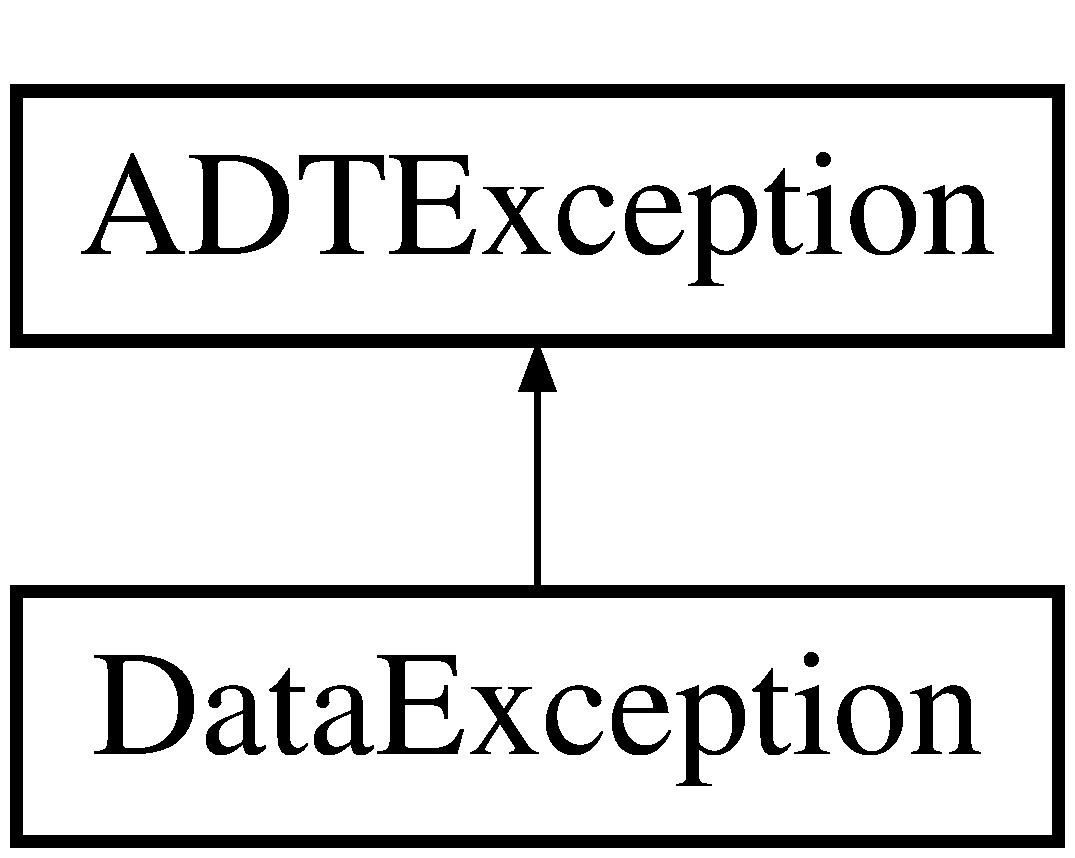
\includegraphics[height=2cm]{classDataException}
\end{center}
\end{figure}
\subsection*{Public Member Functions}
\begin{DoxyCompactItemize}
\item 
virtual \hyperlink{classDataException_a78bbe639df04f97e992fbbdc77f5fc25}{$\sim$DataException} ()
\end{DoxyCompactItemize}
\subsection*{Data Fields}
\begin{DoxyCompactItemize}
\item 
string \hyperlink{classDataException_a8cac3128f4a8d7749d2ffcefa0726aee}{message}
\end{DoxyCompactItemize}


\subsection{Constructor \& Destructor Documentation}
\hypertarget{classDataException_a78bbe639df04f97e992fbbdc77f5fc25}{
\index{DataException@{DataException}!$\sim$DataException@{$\sim$DataException}}
\index{$\sim$DataException@{$\sim$DataException}!DataException@{DataException}}
\subsubsection[{$\sim$DataException}]{\setlength{\rightskip}{0pt plus 5cm}virtual DataException::$\sim$DataException ()\hspace{0.3cm}{\ttfamily  \mbox{[}inline, virtual\mbox{]}}}}
\label{classDataException_a78bbe639df04f97e992fbbdc77f5fc25}


\subsection{Field Documentation}
\hypertarget{classDataException_a8cac3128f4a8d7749d2ffcefa0726aee}{
\index{DataException@{DataException}!message@{message}}
\index{message@{message}!DataException@{DataException}}
\subsubsection[{message}]{\setlength{\rightskip}{0pt plus 5cm}string {\bf DataException::message}}}
\label{classDataException_a8cac3128f4a8d7749d2ffcefa0726aee}


The documentation for this class was generated from the following file:\begin{DoxyCompactItemize}
\item 
engine/utils/\hyperlink{exceptions_8h}{exceptions.h}\end{DoxyCompactItemize}

\hypertarget{classDeterminantCalculationEx}{
\section{DeterminantCalculationEx Class Reference}
\label{classDeterminantCalculationEx}\index{DeterminantCalculationEx@{DeterminantCalculationEx}}
}


{\ttfamily \#include $<$exceptions.h$>$}

Inheritance diagram for DeterminantCalculationEx:\begin{figure}[H]
\begin{center}
\leavevmode
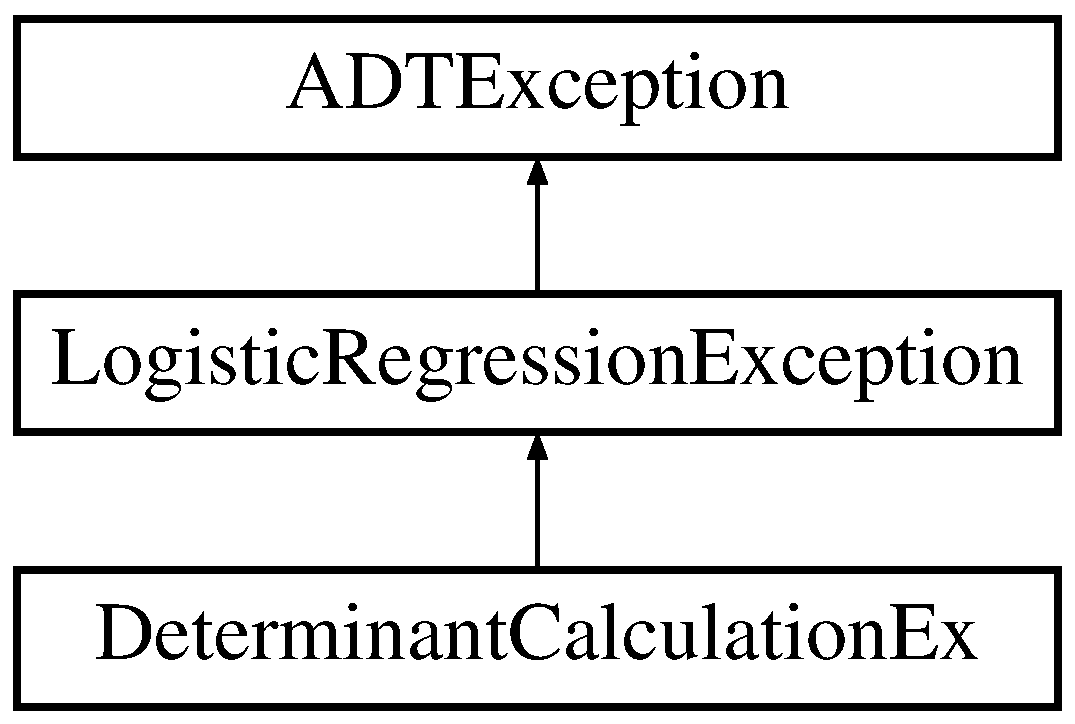
\includegraphics[height=3cm]{classDeterminantCalculationEx}
\end{center}
\end{figure}


The documentation for this class was generated from the following file:\begin{DoxyCompactItemize}
\item 
engine/utils/\hyperlink{exceptions_8h}{exceptions.h}\end{DoxyCompactItemize}

\hypertarget{classEM}{
\section{EM Class Reference}
\label{classEM}\index{EM@{EM}}
}


{\ttfamily \#include $<$em.h$>$}

\subsection*{Public Member Functions}
\begin{DoxyCompactItemize}
\item 
\hyperlink{classEM_ab63fb999a41e57947ecd2e61c073c5ef}{EM} ()
\item 
\hyperlink{classEM_a5da3eaa0aa91b3925de2c5bca158faca}{$\sim$EM} ()
\item 
void \hyperlink{classEM_abcc9e390b2a2c8143bfa364a7911d6fa}{setup} (const vector$<$ vector$<$ short $>$ $>$ \&)
\item 
bool \hyperlink{classEM_a18638c8e6a8da46ca0ea77981c275486}{run} ()
\item 
void \hyperlink{classEM_abe803c5ae01733a57224c3d530ae2921}{result} (double $\ast$$\ast$, vector$<$ int $>$ \&, vector$<$ double $>$ \&)
\item 
void \hyperlink{classEM_ac3787d2909eb87ac231b533482d1f644}{getAlleleFreqs} (double a\mbox{[}2\mbox{]}\mbox{[}3\mbox{]})
\item 
vector$<$ int $>$ \hyperlink{classEM_a5050cd53ebe803ee4e677119af7869ae}{getNumberAlleles} ()
\item 
vector$<$ double $>$ \hyperlink{classEM_ac7552d323bf702bc7a76ade909415cab}{getHapProbs} ()
\item 
vector$<$ double $>$ \hyperlink{classEM_ab5f91b9b53ea2090197c8e389ffa5a38}{getEMFreqs} ()
\item 
vector$<$ \hyperlink{structEMPersonalProbsResults}{EMPersonalProbsResults} $>$ \hyperlink{classEM_a07bb2d56390f494c885bd7c7ea4b53b9}{getPersonalProbabilities} ()
\end{DoxyCompactItemize}
\subsection*{Protected Member Functions}
\begin{DoxyCompactItemize}
\item 
int \hyperlink{classEM_a5393a49dd932245a931e6d5eece1cf27}{uniqueElements} (const vector$<$ short $>$ \&)
\item 
void \hyperlink{classEM_a8531164d0fa92217eb0c7d9f75382912}{initEMAlgorithm} ()
\item 
void \hyperlink{classEM_af7ab6d102b2901761764b91abb28d88a}{computeIncompleteFreqs} ()
\item 
void \hyperlink{classEM_a385df83b9c344ceaa000966dccc92796}{computeCompleteFreqs} ()
\item 
void \hyperlink{classEM_a65fd72ccd0f1a9ff5289e96d419fa65f}{cycleThroughPeople} ()
\item 
void \hyperlink{classEM_addc146c4cd9b7d98e01c485454544529}{distributeCounts} ()
\item 
void \hyperlink{classEM_a7a49c56e4c55158f0c1ff4ec6a9469e3}{reweightKnownHaps} ()
\item 
void \hyperlink{classEM_af63a611b10a4a1bbe15b2013d2c72b45}{getRelHaps} (int indiv, int split, int \&newHapNum1, int \&newHapNum2)
\item 
int \hyperlink{classEM_a456073e2e19b310df9ed0f953dbd6abc}{getRelHap1} (int indiv, int split, vector$<$ int $>$ \&\hyperlink{classEM_a8355d01f8998e654c32b1fc8f478ced1}{numAlleles}) const 
\begin{DoxyCompactList}\small\item\em . Use the combined form. \item\end{DoxyCompactList}\item 
int \hyperlink{classEM_a8a03279b3b78e8f88add021a28b7ac28}{getRelHap2} (int indiv, int split, vector$<$ int $>$ \&\hyperlink{classEM_a8355d01f8998e654c32b1fc8f478ced1}{numAlleles}) const 
\item 
void \hyperlink{classEM_a1bd0c351ef1ee04ad0552f2066d7f3d7}{resolve} (vector$<$ vector$<$ double $>$ $>$ \&, int lefthap, int righthap)
\item 
int \hyperlink{classEM_a3e6b256bb2996b1903f5a2490540659b}{hapToIndex} (const vector$<$ int $>$ \&)
\item 
int \hyperlink{classEM_abdb50dc221b573b78c2c9785b2ae7f9b}{index2Allele} (int imark, int haplotypeIndex)
\end{DoxyCompactItemize}
\subsection*{Protected Attributes}
\begin{DoxyCompactItemize}
\item 
vector$<$ vector$<$ short $>$ $>$ \hyperlink{classEM_a0a7a49feeff6a6ce2908bd626c876a60}{inTotal}
\item 
vector$<$ int $>$ \hyperlink{classEM_a8355d01f8998e654c32b1fc8f478ced1}{numAlleles}
\item 
int \hyperlink{classEM_ae8420599f2bb0359bec3f8640699aa43}{numberAlleles}
\item 
int \hyperlink{classEM_a6fb53f57dafe2497417ae7b55748a2f5}{numHaps}
\item 
int \hyperlink{classEM_af93ac6cc803cd05ab2a266e77b864ae1}{numSplits}
\item 
vector$<$ double $>$ \hyperlink{classEM_adc712759a9c74b26826ffbc28d4cf410}{unknownProb}
\item 
vector$<$ double $>$ \hyperlink{classEM_ae28d8a79298bd3b15801f4eff84216b1}{tempCount}
\item 
vector$<$ double $>$ \hyperlink{classEM_ae76fe505f85355d362d5022436980331}{emFrequencies}
\item 
vector$<$ \hyperlink{classhaplotype}{haplotype} $\ast$ $>$ \hyperlink{classEM_a16a75209aa892c812af91aaea1b41500}{incompleteTable}
\item 
vector$<$ \hyperlink{classhaplotype}{haplotype} $>$ \hyperlink{classEM_a4d771fc7aca0ee55ee0b8742269b54e7}{haplotype1}
\item 
vector$<$ \hyperlink{classhaplotype}{haplotype} $>$ \hyperlink{classEM_a7eb2fa8a9c6db4c1425d77298cec869d}{haplotype2}
\item 
int \hyperlink{classEM_a138450b0d00acac64fd8a272b999be9f}{setFor}
\item 
vector$<$ vector$<$ double $>$ $>$ \hyperlink{classEM_abb7e20d53630eb8b692084ba1cf666c5}{personalProb}
\end{DoxyCompactItemize}
\subsection*{Friends}
\begin{DoxyCompactItemize}
\item 
class \hyperlink{classEM_ab5eb8e85b324a9728c593bdc1ada8198}{HaploStats}
\end{DoxyCompactItemize}


\subsection{Constructor \& Destructor Documentation}
\hypertarget{classEM_ab63fb999a41e57947ecd2e61c073c5ef}{
\index{EM@{EM}!EM@{EM}}
\index{EM@{EM}!EM@{EM}}
\subsubsection[{EM}]{\setlength{\rightskip}{0pt plus 5cm}EM::EM ()}}
\label{classEM_ab63fb999a41e57947ecd2e61c073c5ef}
\hypertarget{classEM_a5da3eaa0aa91b3925de2c5bca158faca}{
\index{EM@{EM}!$\sim$EM@{$\sim$EM}}
\index{$\sim$EM@{$\sim$EM}!EM@{EM}}
\subsubsection[{$\sim$EM}]{\setlength{\rightskip}{0pt plus 5cm}EM::$\sim$EM ()}}
\label{classEM_a5da3eaa0aa91b3925de2c5bca158faca}


\subsection{Member Function Documentation}
\hypertarget{classEM_a385df83b9c344ceaa000966dccc92796}{
\index{EM@{EM}!computeCompleteFreqs@{computeCompleteFreqs}}
\index{computeCompleteFreqs@{computeCompleteFreqs}!EM@{EM}}
\subsubsection[{computeCompleteFreqs}]{\setlength{\rightskip}{0pt plus 5cm}void EM::computeCompleteFreqs ()\hspace{0.3cm}{\ttfamily  \mbox{[}protected\mbox{]}}}}
\label{classEM_a385df83b9c344ceaa000966dccc92796}
\hypertarget{classEM_af7ab6d102b2901761764b91abb28d88a}{
\index{EM@{EM}!computeIncompleteFreqs@{computeIncompleteFreqs}}
\index{computeIncompleteFreqs@{computeIncompleteFreqs}!EM@{EM}}
\subsubsection[{computeIncompleteFreqs}]{\setlength{\rightskip}{0pt plus 5cm}void EM::computeIncompleteFreqs ()\hspace{0.3cm}{\ttfamily  \mbox{[}protected\mbox{]}}}}
\label{classEM_af7ab6d102b2901761764b91abb28d88a}
\hypertarget{classEM_a65fd72ccd0f1a9ff5289e96d419fa65f}{
\index{EM@{EM}!cycleThroughPeople@{cycleThroughPeople}}
\index{cycleThroughPeople@{cycleThroughPeople}!EM@{EM}}
\subsubsection[{cycleThroughPeople}]{\setlength{\rightskip}{0pt plus 5cm}void EM::cycleThroughPeople ()\hspace{0.3cm}{\ttfamily  \mbox{[}protected\mbox{]}}}}
\label{classEM_a65fd72ccd0f1a9ff5289e96d419fa65f}
\hypertarget{classEM_addc146c4cd9b7d98e01c485454544529}{
\index{EM@{EM}!distributeCounts@{distributeCounts}}
\index{distributeCounts@{distributeCounts}!EM@{EM}}
\subsubsection[{distributeCounts}]{\setlength{\rightskip}{0pt plus 5cm}void EM::distributeCounts ()\hspace{0.3cm}{\ttfamily  \mbox{[}protected\mbox{]}}}}
\label{classEM_addc146c4cd9b7d98e01c485454544529}
\hypertarget{classEM_ac3787d2909eb87ac231b533482d1f644}{
\index{EM@{EM}!getAlleleFreqs@{getAlleleFreqs}}
\index{getAlleleFreqs@{getAlleleFreqs}!EM@{EM}}
\subsubsection[{getAlleleFreqs}]{\setlength{\rightskip}{0pt plus 5cm}void EM::getAlleleFreqs (double {\em a}\mbox{[}2\mbox{]}\mbox{[}3\mbox{]})}}
\label{classEM_ac3787d2909eb87ac231b533482d1f644}
\hypertarget{classEM_ab5f91b9b53ea2090197c8e389ffa5a38}{
\index{EM@{EM}!getEMFreqs@{getEMFreqs}}
\index{getEMFreqs@{getEMFreqs}!EM@{EM}}
\subsubsection[{getEMFreqs}]{\setlength{\rightskip}{0pt plus 5cm}vector$<$ double $>$ EM::getEMFreqs ()}}
\label{classEM_ab5f91b9b53ea2090197c8e389ffa5a38}
Return the haplotype frequencies for each possible haplotype. \hypertarget{classEM_ac7552d323bf702bc7a76ade909415cab}{
\index{EM@{EM}!getHapProbs@{getHapProbs}}
\index{getHapProbs@{getHapProbs}!EM@{EM}}
\subsubsection[{getHapProbs}]{\setlength{\rightskip}{0pt plus 5cm}vector$<$ double $>$ EM::getHapProbs ()}}
\label{classEM_ac7552d323bf702bc7a76ade909415cab}
\hypertarget{classEM_a5050cd53ebe803ee4e677119af7869ae}{
\index{EM@{EM}!getNumberAlleles@{getNumberAlleles}}
\index{getNumberAlleles@{getNumberAlleles}!EM@{EM}}
\subsubsection[{getNumberAlleles}]{\setlength{\rightskip}{0pt plus 5cm}vector$<$ int $>$ EM::getNumberAlleles ()}}
\label{classEM_a5050cd53ebe803ee4e677119af7869ae}
\hypertarget{classEM_a07bb2d56390f494c885bd7c7ea4b53b9}{
\index{EM@{EM}!getPersonalProbabilities@{getPersonalProbabilities}}
\index{getPersonalProbabilities@{getPersonalProbabilities}!EM@{EM}}
\subsubsection[{getPersonalProbabilities}]{\setlength{\rightskip}{0pt plus 5cm}vector$<$ {\bf EMPersonalProbsResults} $>$ EM::getPersonalProbabilities ()}}
\label{classEM_a07bb2d56390f494c885bd7c7ea4b53b9}
Calculate all haplotype probs for an individual. \hypertarget{classEM_a456073e2e19b310df9ed0f953dbd6abc}{
\index{EM@{EM}!getRelHap1@{getRelHap1}}
\index{getRelHap1@{getRelHap1}!EM@{EM}}
\subsubsection[{getRelHap1}]{\setlength{\rightskip}{0pt plus 5cm}int EM::getRelHap1 (int {\em indiv}, \/  int {\em split}, \/  vector$<$ int $>$ \& {\em numAlleles}) const\hspace{0.3cm}{\ttfamily  \mbox{[}protected\mbox{]}}}}
\label{classEM_a456073e2e19b310df9ed0f953dbd6abc}


. Use the combined form. 

\hypertarget{classEM_a8a03279b3b78e8f88add021a28b7ac28}{
\index{EM@{EM}!getRelHap2@{getRelHap2}}
\index{getRelHap2@{getRelHap2}!EM@{EM}}
\subsubsection[{getRelHap2}]{\setlength{\rightskip}{0pt plus 5cm}int EM::getRelHap2 (int {\em indiv}, \/  int {\em split}, \/  vector$<$ int $>$ \& {\em numAlleles}) const\hspace{0.3cm}{\ttfamily  \mbox{[}protected\mbox{]}}}}
\label{classEM_a8a03279b3b78e8f88add021a28b7ac28}
\hypertarget{classEM_af63a611b10a4a1bbe15b2013d2c72b45}{
\index{EM@{EM}!getRelHaps@{getRelHaps}}
\index{getRelHaps@{getRelHaps}!EM@{EM}}
\subsubsection[{getRelHaps}]{\setlength{\rightskip}{0pt plus 5cm}void EM::getRelHaps (int {\em indiv}, \/  int {\em split}, \/  int \& {\em newHapNum1}, \/  int \& {\em newHapNum2})\hspace{0.3cm}{\ttfamily  \mbox{[}protected\mbox{]}}}}
\label{classEM_af63a611b10a4a1bbe15b2013d2c72b45}
\hypertarget{classEM_a3e6b256bb2996b1903f5a2490540659b}{
\index{EM@{EM}!hapToIndex@{hapToIndex}}
\index{hapToIndex@{hapToIndex}!EM@{EM}}
\subsubsection[{hapToIndex}]{\setlength{\rightskip}{0pt plus 5cm}int EM::hapToIndex (const vector$<$ int $>$ \& {\em haps})\hspace{0.3cm}{\ttfamily  \mbox{[}protected\mbox{]}}}}
\label{classEM_a3e6b256bb2996b1903f5a2490540659b}
\hypertarget{classEM_abdb50dc221b573b78c2c9785b2ae7f9b}{
\index{EM@{EM}!index2Allele@{index2Allele}}
\index{index2Allele@{index2Allele}!EM@{EM}}
\subsubsection[{index2Allele}]{\setlength{\rightskip}{0pt plus 5cm}int EM::index2Allele (int {\em imark}, \/  int {\em haplotypeIndex})\hspace{0.3cm}{\ttfamily  \mbox{[}protected\mbox{]}}}}
\label{classEM_abdb50dc221b573b78c2c9785b2ae7f9b}
\hypertarget{classEM_a8531164d0fa92217eb0c7d9f75382912}{
\index{EM@{EM}!initEMAlgorithm@{initEMAlgorithm}}
\index{initEMAlgorithm@{initEMAlgorithm}!EM@{EM}}
\subsubsection[{initEMAlgorithm}]{\setlength{\rightskip}{0pt plus 5cm}void EM::initEMAlgorithm ()\hspace{0.3cm}{\ttfamily  \mbox{[}protected\mbox{]}}}}
\label{classEM_a8531164d0fa92217eb0c7d9f75382912}
Perform initilization for the \hyperlink{classEM}{EM} by giving all haplotypes equal probability \hypertarget{classEM_a1bd0c351ef1ee04ad0552f2066d7f3d7}{
\index{EM@{EM}!resolve@{resolve}}
\index{resolve@{resolve}!EM@{EM}}
\subsubsection[{resolve}]{\setlength{\rightskip}{0pt plus 5cm}void EM::resolve (vector$<$ vector$<$ double $>$ $>$ \& {\em personalProb}, \/  int {\em lefthap}, \/  int {\em righthap})\hspace{0.3cm}{\ttfamily  \mbox{[}protected\mbox{]}}}}
\label{classEM_a1bd0c351ef1ee04ad0552f2066d7f3d7}
\hypertarget{classEM_abe803c5ae01733a57224c3d530ae2921}{
\index{EM@{EM}!result@{result}}
\index{result@{result}!EM@{EM}}
\subsubsection[{result}]{\setlength{\rightskip}{0pt plus 5cm}void EM::result (double $\ast$$\ast$ {\em aFreq}, \/  vector$<$ int $>$ \& {\em numAlleles}, \/  vector$<$ double $>$ \& {\em hapProbs})}}
\label{classEM_abe803c5ae01733a57224c3d530ae2921}
\hypertarget{classEM_a7a49c56e4c55158f0c1ff4ec6a9469e3}{
\index{EM@{EM}!reweightKnownHaps@{reweightKnownHaps}}
\index{reweightKnownHaps@{reweightKnownHaps}!EM@{EM}}
\subsubsection[{reweightKnownHaps}]{\setlength{\rightskip}{0pt plus 5cm}void EM::reweightKnownHaps ()\hspace{0.3cm}{\ttfamily  \mbox{[}protected\mbox{]}}}}
\label{classEM_a7a49c56e4c55158f0c1ff4ec6a9469e3}
\hypertarget{classEM_a18638c8e6a8da46ca0ea77981c275486}{
\index{EM@{EM}!run@{run}}
\index{run@{run}!EM@{EM}}
\subsubsection[{run}]{\setlength{\rightskip}{0pt plus 5cm}bool EM::run ()}}
\label{classEM_a18638c8e6a8da46ca0ea77981c275486}
Execute the \hyperlink{classEM}{EM} algorithm for the individuals that have been loaded. \hypertarget{classEM_abcc9e390b2a2c8143bfa364a7911d6fa}{
\index{EM@{EM}!setup@{setup}}
\index{setup@{setup}!EM@{EM}}
\subsubsection[{setup}]{\setlength{\rightskip}{0pt plus 5cm}void EM::setup (const vector$<$ vector$<$ short $>$ $>$ \& {\em data})}}
\label{classEM_abcc9e390b2a2c8143bfa364a7911d6fa}
Perform the initilization steps to run on an arbitrary number of individuals.


\begin{DoxyParams}{Parameters}
\item[{\em \&data}]Each inner vector is a SNP. \end{DoxyParams}
\hypertarget{classEM_a5393a49dd932245a931e6d5eece1cf27}{
\index{EM@{EM}!uniqueElements@{uniqueElements}}
\index{uniqueElements@{uniqueElements}!EM@{EM}}
\subsubsection[{uniqueElements}]{\setlength{\rightskip}{0pt plus 5cm}int EM::uniqueElements (const vector$<$ short $>$ \& {\em v})\hspace{0.3cm}{\ttfamily  \mbox{[}protected\mbox{]}}}}
\label{classEM_a5393a49dd932245a931e6d5eece1cf27}


\subsection{Friends And Related Function Documentation}
\hypertarget{classEM_ab5eb8e85b324a9728c593bdc1ada8198}{
\index{EM@{EM}!HaploStats@{HaploStats}}
\index{HaploStats@{HaploStats}!EM@{EM}}
\subsubsection[{HaploStats}]{\setlength{\rightskip}{0pt plus 5cm}friend class {\bf HaploStats}\hspace{0.3cm}{\ttfamily  \mbox{[}friend\mbox{]}}}}
\label{classEM_ab5eb8e85b324a9728c593bdc1ada8198}


\subsection{Field Documentation}
\hypertarget{classEM_ae76fe505f85355d362d5022436980331}{
\index{EM@{EM}!emFrequencies@{emFrequencies}}
\index{emFrequencies@{emFrequencies}!EM@{EM}}
\subsubsection[{emFrequencies}]{\setlength{\rightskip}{0pt plus 5cm}vector$<$double$>$ {\bf EM::emFrequencies}\hspace{0.3cm}{\ttfamily  \mbox{[}protected\mbox{]}}}}
\label{classEM_ae76fe505f85355d362d5022436980331}
\hypertarget{classEM_a4d771fc7aca0ee55ee0b8742269b54e7}{
\index{EM@{EM}!haplotype1@{haplotype1}}
\index{haplotype1@{haplotype1}!EM@{EM}}
\subsubsection[{haplotype1}]{\setlength{\rightskip}{0pt plus 5cm}vector$<${\bf haplotype}$>$ {\bf EM::haplotype1}\hspace{0.3cm}{\ttfamily  \mbox{[}protected\mbox{]}}}}
\label{classEM_a4d771fc7aca0ee55ee0b8742269b54e7}
\hypertarget{classEM_a7eb2fa8a9c6db4c1425d77298cec869d}{
\index{EM@{EM}!haplotype2@{haplotype2}}
\index{haplotype2@{haplotype2}!EM@{EM}}
\subsubsection[{haplotype2}]{\setlength{\rightskip}{0pt plus 5cm}vector$<${\bf haplotype}$>$ {\bf EM::haplotype2}\hspace{0.3cm}{\ttfamily  \mbox{[}protected\mbox{]}}}}
\label{classEM_a7eb2fa8a9c6db4c1425d77298cec869d}
\hypertarget{classEM_a16a75209aa892c812af91aaea1b41500}{
\index{EM@{EM}!incompleteTable@{incompleteTable}}
\index{incompleteTable@{incompleteTable}!EM@{EM}}
\subsubsection[{incompleteTable}]{\setlength{\rightskip}{0pt plus 5cm}vector$<${\bf haplotype} $\ast$$>$ {\bf EM::incompleteTable}\hspace{0.3cm}{\ttfamily  \mbox{[}protected\mbox{]}}}}
\label{classEM_a16a75209aa892c812af91aaea1b41500}
\hypertarget{classEM_a0a7a49feeff6a6ce2908bd626c876a60}{
\index{EM@{EM}!inTotal@{inTotal}}
\index{inTotal@{inTotal}!EM@{EM}}
\subsubsection[{inTotal}]{\setlength{\rightskip}{0pt plus 5cm}vector$<$vector$<$short$>$ $>$ {\bf EM::inTotal}\hspace{0.3cm}{\ttfamily  \mbox{[}protected\mbox{]}}}}
\label{classEM_a0a7a49feeff6a6ce2908bd626c876a60}
\hypertarget{classEM_a8355d01f8998e654c32b1fc8f478ced1}{
\index{EM@{EM}!numAlleles@{numAlleles}}
\index{numAlleles@{numAlleles}!EM@{EM}}
\subsubsection[{numAlleles}]{\setlength{\rightskip}{0pt plus 5cm}vector$<$int$>$ {\bf EM::numAlleles}\hspace{0.3cm}{\ttfamily  \mbox{[}protected\mbox{]}}}}
\label{classEM_a8355d01f8998e654c32b1fc8f478ced1}
\hypertarget{classEM_ae8420599f2bb0359bec3f8640699aa43}{
\index{EM@{EM}!numberAlleles@{numberAlleles}}
\index{numberAlleles@{numberAlleles}!EM@{EM}}
\subsubsection[{numberAlleles}]{\setlength{\rightskip}{0pt plus 5cm}int {\bf EM::numberAlleles}\hspace{0.3cm}{\ttfamily  \mbox{[}protected\mbox{]}}}}
\label{classEM_ae8420599f2bb0359bec3f8640699aa43}
\hypertarget{classEM_a6fb53f57dafe2497417ae7b55748a2f5}{
\index{EM@{EM}!numHaps@{numHaps}}
\index{numHaps@{numHaps}!EM@{EM}}
\subsubsection[{numHaps}]{\setlength{\rightskip}{0pt plus 5cm}int {\bf EM::numHaps}\hspace{0.3cm}{\ttfamily  \mbox{[}protected\mbox{]}}}}
\label{classEM_a6fb53f57dafe2497417ae7b55748a2f5}
\hypertarget{classEM_af93ac6cc803cd05ab2a266e77b864ae1}{
\index{EM@{EM}!numSplits@{numSplits}}
\index{numSplits@{numSplits}!EM@{EM}}
\subsubsection[{numSplits}]{\setlength{\rightskip}{0pt plus 5cm}int {\bf EM::numSplits}\hspace{0.3cm}{\ttfamily  \mbox{[}protected\mbox{]}}}}
\label{classEM_af93ac6cc803cd05ab2a266e77b864ae1}
\hypertarget{classEM_abb7e20d53630eb8b692084ba1cf666c5}{
\index{EM@{EM}!personalProb@{personalProb}}
\index{personalProb@{personalProb}!EM@{EM}}
\subsubsection[{personalProb}]{\setlength{\rightskip}{0pt plus 5cm}vector$<$vector$<$double$>$ $>$ {\bf EM::personalProb}\hspace{0.3cm}{\ttfamily  \mbox{[}protected\mbox{]}}}}
\label{classEM_abb7e20d53630eb8b692084ba1cf666c5}
\hypertarget{classEM_a138450b0d00acac64fd8a272b999be9f}{
\index{EM@{EM}!setFor@{setFor}}
\index{setFor@{setFor}!EM@{EM}}
\subsubsection[{setFor}]{\setlength{\rightskip}{0pt plus 5cm}int {\bf EM::setFor}\hspace{0.3cm}{\ttfamily  \mbox{[}protected\mbox{]}}}}
\label{classEM_a138450b0d00acac64fd8a272b999be9f}
\hypertarget{classEM_ae28d8a79298bd3b15801f4eff84216b1}{
\index{EM@{EM}!tempCount@{tempCount}}
\index{tempCount@{tempCount}!EM@{EM}}
\subsubsection[{tempCount}]{\setlength{\rightskip}{0pt plus 5cm}vector$<$double$>$ {\bf EM::tempCount}\hspace{0.3cm}{\ttfamily  \mbox{[}protected\mbox{]}}}}
\label{classEM_ae28d8a79298bd3b15801f4eff84216b1}
\hypertarget{classEM_adc712759a9c74b26826ffbc28d4cf410}{
\index{EM@{EM}!unknownProb@{unknownProb}}
\index{unknownProb@{unknownProb}!EM@{EM}}
\subsubsection[{unknownProb}]{\setlength{\rightskip}{0pt plus 5cm}vector$<$double$>$ {\bf EM::unknownProb}\hspace{0.3cm}{\ttfamily  \mbox{[}protected\mbox{]}}}}
\label{classEM_adc712759a9c74b26826ffbc28d4cf410}


The documentation for this class was generated from the following files:\begin{DoxyCompactItemize}
\item 
engine/em/\hyperlink{em_8h}{em.h}\item 
engine/em/\hyperlink{em_8cpp}{em.cpp}\end{DoxyCompactItemize}

\hypertarget{classEMAlgorithmFailureException}{
\section{EMAlgorithmFailureException Class Reference}
\label{classEMAlgorithmFailureException}\index{EMAlgorithmFailureException@{EMAlgorithmFailureException}}
}


{\ttfamily \#include $<$exceptions.h$>$}

Inheritance diagram for EMAlgorithmFailureException:\begin{figure}[H]
\begin{center}
\leavevmode
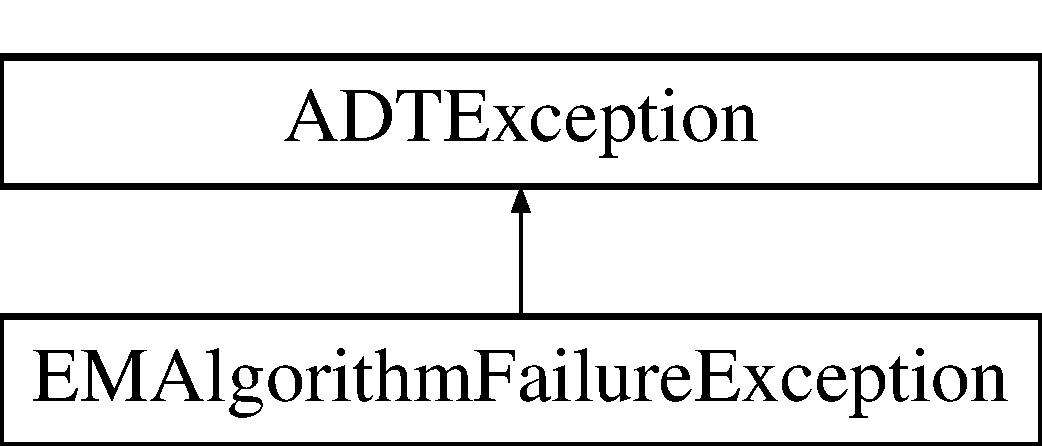
\includegraphics[height=2cm]{classEMAlgorithmFailureException}
\end{center}
\end{figure}


The documentation for this class was generated from the following file:\begin{DoxyCompactItemize}
\item 
engine/utils/\hyperlink{exceptions_8h}{exceptions.h}\end{DoxyCompactItemize}

\hypertarget{classEMAlgorithmNoSetup}{
\section{EMAlgorithmNoSetup Class Reference}
\label{classEMAlgorithmNoSetup}\index{EMAlgorithmNoSetup@{EMAlgorithmNoSetup}}
}


{\ttfamily \#include $<$exceptions.h$>$}

Inheritance diagram for EMAlgorithmNoSetup:\begin{figure}[H]
\begin{center}
\leavevmode
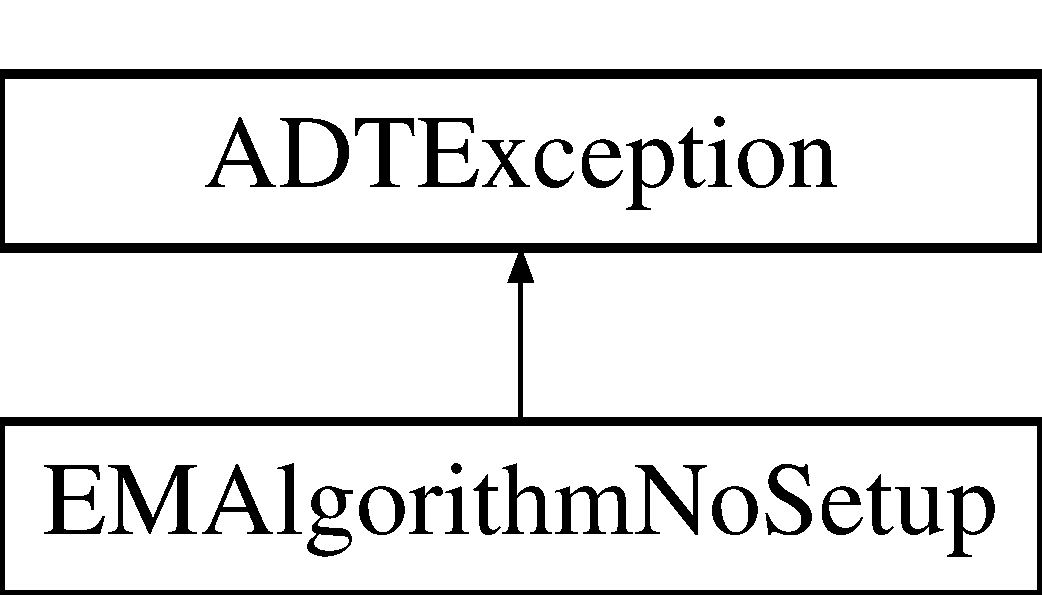
\includegraphics[height=2cm]{classEMAlgorithmNoSetup}
\end{center}
\end{figure}


The documentation for this class was generated from the following file:\begin{DoxyCompactItemize}
\item 
engine/utils/\hyperlink{exceptions_8h}{exceptions.h}\end{DoxyCompactItemize}

\hypertarget{classEMAlgorithmRunResultsMismatch}{
\section{EMAlgorithmRunResultsMismatch Class Reference}
\label{classEMAlgorithmRunResultsMismatch}\index{EMAlgorithmRunResultsMismatch@{EMAlgorithmRunResultsMismatch}}
}


{\ttfamily \#include $<$exceptions.h$>$}

Inheritance diagram for EMAlgorithmRunResultsMismatch:\begin{figure}[H]
\begin{center}
\leavevmode
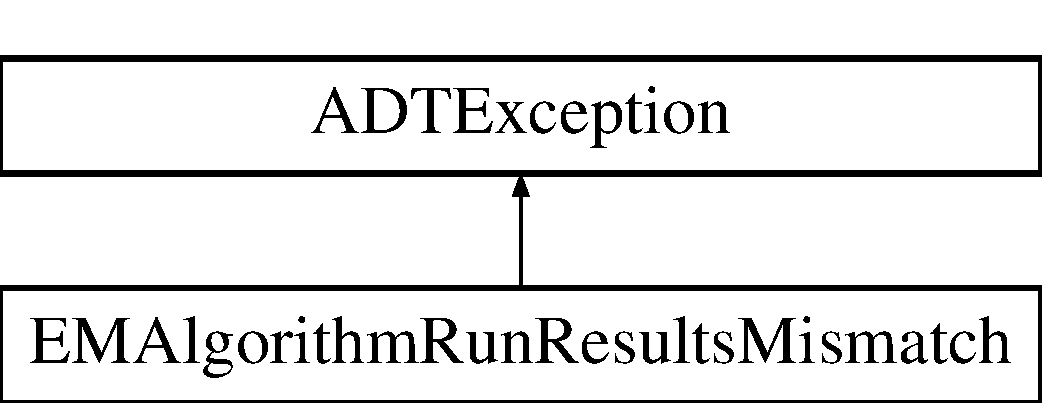
\includegraphics[height=2cm]{classEMAlgorithmRunResultsMismatch}
\end{center}
\end{figure}


The documentation for this class was generated from the following file:\begin{DoxyCompactItemize}
\item 
engine/utils/\hyperlink{exceptions_8h}{exceptions.h}\end{DoxyCompactItemize}

\hypertarget{structEMPersonalProbsResults}{
\section{EMPersonalProbsResults Struct Reference}
\label{structEMPersonalProbsResults}\index{EMPersonalProbsResults@{EMPersonalProbsResults}}
}


{\ttfamily \#include $<$em.h$>$}

\subsection*{Data Fields}
\begin{DoxyCompactItemize}
\item 
int \hyperlink{structEMPersonalProbsResults_ad656d2e7ccb659689b21016c28b58ff4}{personId}
\item 
int \hyperlink{structEMPersonalProbsResults_ae4a36f80c0146b7c5b712fb2d6d71138}{leftHap}
\item 
int \hyperlink{structEMPersonalProbsResults_a3bacb2357ef66f91aeb3feffe1666e92}{rightHap}
\item 
double \hyperlink{structEMPersonalProbsResults_ae9e07e1bcc31ff1622b96dcc8f5e86d1}{prob}
\end{DoxyCompactItemize}


\subsection{Field Documentation}
\hypertarget{structEMPersonalProbsResults_ae4a36f80c0146b7c5b712fb2d6d71138}{
\index{EMPersonalProbsResults@{EMPersonalProbsResults}!leftHap@{leftHap}}
\index{leftHap@{leftHap}!EMPersonalProbsResults@{EMPersonalProbsResults}}
\subsubsection[{leftHap}]{\setlength{\rightskip}{0pt plus 5cm}int {\bf EMPersonalProbsResults::leftHap}}}
\label{structEMPersonalProbsResults_ae4a36f80c0146b7c5b712fb2d6d71138}
\hypertarget{structEMPersonalProbsResults_ad656d2e7ccb659689b21016c28b58ff4}{
\index{EMPersonalProbsResults@{EMPersonalProbsResults}!personId@{personId}}
\index{personId@{personId}!EMPersonalProbsResults@{EMPersonalProbsResults}}
\subsubsection[{personId}]{\setlength{\rightskip}{0pt plus 5cm}int {\bf EMPersonalProbsResults::personId}}}
\label{structEMPersonalProbsResults_ad656d2e7ccb659689b21016c28b58ff4}
\hypertarget{structEMPersonalProbsResults_ae9e07e1bcc31ff1622b96dcc8f5e86d1}{
\index{EMPersonalProbsResults@{EMPersonalProbsResults}!prob@{prob}}
\index{prob@{prob}!EMPersonalProbsResults@{EMPersonalProbsResults}}
\subsubsection[{prob}]{\setlength{\rightskip}{0pt plus 5cm}double {\bf EMPersonalProbsResults::prob}}}
\label{structEMPersonalProbsResults_ae9e07e1bcc31ff1622b96dcc8f5e86d1}
\hypertarget{structEMPersonalProbsResults_a3bacb2357ef66f91aeb3feffe1666e92}{
\index{EMPersonalProbsResults@{EMPersonalProbsResults}!rightHap@{rightHap}}
\index{rightHap@{rightHap}!EMPersonalProbsResults@{EMPersonalProbsResults}}
\subsubsection[{rightHap}]{\setlength{\rightskip}{0pt plus 5cm}int {\bf EMPersonalProbsResults::rightHap}}}
\label{structEMPersonalProbsResults_a3bacb2357ef66f91aeb3feffe1666e92}


The documentation for this struct was generated from the following file:\begin{DoxyCompactItemize}
\item 
engine/em/\hyperlink{em_8h}{em.h}\end{DoxyCompactItemize}

\hypertarget{classEngine}{
\section{Engine Class Reference}
\label{classEngine}\index{Engine@{Engine}}
}


{\ttfamily \#include $<$engine.h$>$}

Inheritance diagram for Engine:\begin{figure}[H]
\begin{center}
\leavevmode
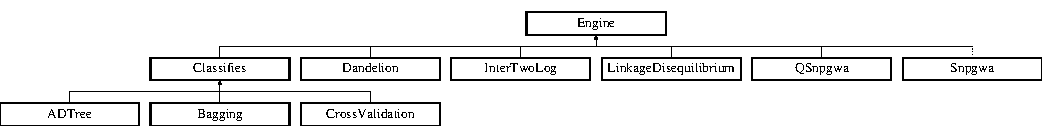
\includegraphics[height=1.69014cm]{classEngine}
\end{center}
\end{figure}
\subsection*{Public Member Functions}
\begin{DoxyCompactItemize}
\item 
virtual void \hyperlink{classEngine_aaa054d596fb8ced6e3eb4bee208f8c3d}{init} ()=0
\item 
virtual void \hyperlink{classEngine_aec7076b8979a13c96eceb362437dc68c}{preProcess} ()=0
\item 
virtual void \hyperlink{classEngine_a005f8e277c3dea16ea05803fba223db7}{process} ()=0
\item 
virtual void \hyperlink{classEngine_a023e094182312b1732fe53754c2fe5cb}{enslave} (\hyperlink{classEngineParamReader}{EngineParamReader} $\ast$)=0
\item 
virtual void \hyperlink{classEngine_a2927c4a4263809453063ad482c6434a4}{test} ()=0
\item 
virtual \hyperlink{classEngine_a41f2d854040e17d9c4d7b324a4bfbf39}{$\sim$Engine} ()
\end{DoxyCompactItemize}
\subsection*{Protected Attributes}
\begin{DoxyCompactItemize}
\item 
\hyperlink{classReader}{Reader} $\ast$ \hyperlink{classEngine_ab8f643f38543ba32dd856f15aa7899e8}{reader}
\item 
\hyperlink{classParamReader}{ParamReader} $\ast$ \hyperlink{classEngine_aa2b8bf8e8a8854d1eacda6bb1a4f4f37}{param\_\-reader}
\item 
\hyperlink{classDataAccess}{DataAccess} $\ast$ \hyperlink{classEngine_a92dad538992bac19762f6cc2a754962a}{data}
\end{DoxyCompactItemize}


\subsection{Detailed Description}
Abstract class for an engine. An engine is a large algorithm class like SNPGWA, INTERTWOLOG, ADTREE, or ADTREEBAG 

\subsection{Constructor \& Destructor Documentation}
\hypertarget{classEngine_a41f2d854040e17d9c4d7b324a4bfbf39}{
\index{Engine@{Engine}!$\sim$Engine@{$\sim$Engine}}
\index{$\sim$Engine@{$\sim$Engine}!Engine@{Engine}}
\subsubsection[{$\sim$Engine}]{\setlength{\rightskip}{0pt plus 5cm}virtual Engine::$\sim$Engine ()\hspace{0.3cm}{\ttfamily  \mbox{[}inline, virtual\mbox{]}}}}
\label{classEngine_a41f2d854040e17d9c4d7b324a4bfbf39}


\subsection{Member Function Documentation}
\hypertarget{classEngine_a023e094182312b1732fe53754c2fe5cb}{
\index{Engine@{Engine}!enslave@{enslave}}
\index{enslave@{enslave}!Engine@{Engine}}
\subsubsection[{enslave}]{\setlength{\rightskip}{0pt plus 5cm}virtual void Engine::enslave ({\bf EngineParamReader} $\ast$)\hspace{0.3cm}{\ttfamily  \mbox{[}pure virtual\mbox{]}}}}
\label{classEngine_a023e094182312b1732fe53754c2fe5cb}


Implemented in \hyperlink{classADTree_a4e89d611e7dc79fa8826efa742f9ce42}{ADTree}, \hyperlink{classBagging_aa1f58fca264385a46fa7c14a5620488c}{Bagging}, \hyperlink{classCrossValidation_a50b65a606c324404de92f44dba655154}{CrossValidation}, \hyperlink{classDandelion_ac95a20aaaff8170c4539e047cb7a551a}{Dandelion}, \hyperlink{classInterTwoLog_aa96d91206c19b781d222f0d6e13bf51d}{InterTwoLog}, \hyperlink{classLinkageDisequilibrium_afb777d3a63bbb0f2d23ce052de891023}{LinkageDisequilibrium}, \hyperlink{classQSnpgwa_a2c39271b1001005e6d5a451dbc2fd8bb}{QSnpgwa}, and \hyperlink{classSnpgwa_a976e974bf71743c194a9c098cefff04c}{Snpgwa}.

\hypertarget{classEngine_aaa054d596fb8ced6e3eb4bee208f8c3d}{
\index{Engine@{Engine}!init@{init}}
\index{init@{init}!Engine@{Engine}}
\subsubsection[{init}]{\setlength{\rightskip}{0pt plus 5cm}virtual void Engine::init ()\hspace{0.3cm}{\ttfamily  \mbox{[}pure virtual\mbox{]}}}}
\label{classEngine_aaa054d596fb8ced6e3eb4bee208f8c3d}


Implemented in \hyperlink{classADTree_a70b34e300c187fb817bc6d8ba31aceaa}{ADTree}, \hyperlink{classBagging_ab58c678f776356ae4b4c1c41dcdf3778}{Bagging}, \hyperlink{classCrossValidation_acf88bf85dec8d27f6aa97d9ec04ccf26}{CrossValidation}, \hyperlink{classDandelion_a6c58019c7b1d8fb5a80c2031afb01374}{Dandelion}, \hyperlink{classInterTwoLog_af5dbc57497069c182c6101211fe2b64a}{InterTwoLog}, \hyperlink{classLinkageDisequilibrium_a9d3c50f9b7c3f5739ce12eb0b2068c6c}{LinkageDisequilibrium}, \hyperlink{classQSnpgwa_ac228fcbfcba981d48a223e911673e406}{QSnpgwa}, and \hyperlink{classSnpgwa_a4d061e98cd1a9b5d9f7d666dea3cd0af}{Snpgwa}.

\hypertarget{classEngine_aec7076b8979a13c96eceb362437dc68c}{
\index{Engine@{Engine}!preProcess@{preProcess}}
\index{preProcess@{preProcess}!Engine@{Engine}}
\subsubsection[{preProcess}]{\setlength{\rightskip}{0pt plus 5cm}virtual void Engine::preProcess ()\hspace{0.3cm}{\ttfamily  \mbox{[}pure virtual\mbox{]}}}}
\label{classEngine_aec7076b8979a13c96eceb362437dc68c}


Implemented in \hyperlink{classADTree_a18b7ad4befedb9073a83c39106628d3b}{ADTree}, \hyperlink{classBagging_a638e97695ee9a685cfee7ce459c2b8f8}{Bagging}, \hyperlink{classCrossValidation_ad45dad478f034a39696660d7c93b34fa}{CrossValidation}, \hyperlink{classDandelion_a21fa4068a4293d3c5068d53627e49393}{Dandelion}, \hyperlink{classInterTwoLog_a581fcf71571bce5c0861e963c16f220b}{InterTwoLog}, \hyperlink{classLinkageDisequilibrium_a2f466153298f2c868a78b5573f6c5048}{LinkageDisequilibrium}, \hyperlink{classQSnpgwa_acc9e7d7e48d9c3e2fbb0a75e263f0c50}{QSnpgwa}, and \hyperlink{classSnpgwa_aa20dc165d74036ff401ca182f5e980c2}{Snpgwa}.

\hypertarget{classEngine_a005f8e277c3dea16ea05803fba223db7}{
\index{Engine@{Engine}!process@{process}}
\index{process@{process}!Engine@{Engine}}
\subsubsection[{process}]{\setlength{\rightskip}{0pt plus 5cm}virtual void Engine::process ()\hspace{0.3cm}{\ttfamily  \mbox{[}pure virtual\mbox{]}}}}
\label{classEngine_a005f8e277c3dea16ea05803fba223db7}


Implemented in \hyperlink{classADTree_acbdd5c7a248305933868e00bd875fd33}{ADTree}, \hyperlink{classBagging_ab732c0768147c13071d4fc23d879dfd4}{Bagging}, \hyperlink{classCrossValidation_a3435a227d91e03af7d1df7e2c6c4fce9}{CrossValidation}, \hyperlink{classDandelion_a3de169eab0899f277a3747a57c94bb0b}{Dandelion}, \hyperlink{classInterTwoLog_abd4e1bdf33314432d4a57193de056905}{InterTwoLog}, \hyperlink{classLinkageDisequilibrium_a821abc8314c8e6bddc1dfcdf24bdda09}{LinkageDisequilibrium}, \hyperlink{classQSnpgwa_a4873c7584d427c41a01e1bba159cf486}{QSnpgwa}, and \hyperlink{classSnpgwa_a0d01afdbda7f3bb32586962cca76b69a}{Snpgwa}.

\hypertarget{classEngine_a2927c4a4263809453063ad482c6434a4}{
\index{Engine@{Engine}!test@{test}}
\index{test@{test}!Engine@{Engine}}
\subsubsection[{test}]{\setlength{\rightskip}{0pt plus 5cm}virtual void Engine::test ()\hspace{0.3cm}{\ttfamily  \mbox{[}pure virtual\mbox{]}}}}
\label{classEngine_a2927c4a4263809453063ad482c6434a4}


Implemented in \hyperlink{classADTree_ac4183a7e36602b90e36e3717deef102c}{ADTree}, \hyperlink{classBagging_afd3022e8be01cba7f97fc9f81cda8016}{Bagging}, \hyperlink{classCrossValidation_a1b4664d9123d676b778ff0e89379a1ba}{CrossValidation}, \hyperlink{classDandelion_aad49aeddeaaf1aa98da869d94777e130}{Dandelion}, \hyperlink{classInterTwoLog_a525b88900b11ed13cdefd73f5024e2eb}{InterTwoLog}, \hyperlink{classLinkageDisequilibrium_a8df37823ab11776642f571e8e8ba7e3b}{LinkageDisequilibrium}, \hyperlink{classQSnpgwa_aa127cdd0a042058f1ecab33d831a58a6}{QSnpgwa}, and \hyperlink{classSnpgwa_af5ea7279e2d31bc5f05a1fc6cd4ef17e}{Snpgwa}.



\subsection{Field Documentation}
\hypertarget{classEngine_a92dad538992bac19762f6cc2a754962a}{
\index{Engine@{Engine}!data@{data}}
\index{data@{data}!Engine@{Engine}}
\subsubsection[{data}]{\setlength{\rightskip}{0pt plus 5cm}{\bf DataAccess}$\ast$ {\bf Engine::data}\hspace{0.3cm}{\ttfamily  \mbox{[}protected\mbox{]}}}}
\label{classEngine_a92dad538992bac19762f6cc2a754962a}
\hypertarget{classEngine_aa2b8bf8e8a8854d1eacda6bb1a4f4f37}{
\index{Engine@{Engine}!param\_\-reader@{param\_\-reader}}
\index{param\_\-reader@{param\_\-reader}!Engine@{Engine}}
\subsubsection[{param\_\-reader}]{\setlength{\rightskip}{0pt plus 5cm}{\bf ParamReader}$\ast$ {\bf Engine::param\_\-reader}\hspace{0.3cm}{\ttfamily  \mbox{[}protected\mbox{]}}}}
\label{classEngine_aa2b8bf8e8a8854d1eacda6bb1a4f4f37}
\hypertarget{classEngine_ab8f643f38543ba32dd856f15aa7899e8}{
\index{Engine@{Engine}!reader@{reader}}
\index{reader@{reader}!Engine@{Engine}}
\subsubsection[{reader}]{\setlength{\rightskip}{0pt plus 5cm}{\bf Reader}$\ast$ {\bf Engine::reader}\hspace{0.3cm}{\ttfamily  \mbox{[}protected\mbox{]}}}}
\label{classEngine_ab8f643f38543ba32dd856f15aa7899e8}


The documentation for this class was generated from the following file:\begin{DoxyCompactItemize}
\item 
engine/\hyperlink{engine_8h}{engine.h}\end{DoxyCompactItemize}

\hypertarget{classEngineParamReader}{
\section{EngineParamReader Class Reference}
\label{classEngineParamReader}\index{EngineParamReader@{EngineParamReader}}
}


{\ttfamily \#include $<$engine\_\-param\_\-reader.h$>$}

\subsection*{Public Types}
\begin{DoxyCompactItemize}
\item 
enum \hyperlink{classEngineParamReader_ab2ee80aa67ba657beddf852c526e1a3d}{BaggingTypes} \{ \hyperlink{classEngineParamReader_ab2ee80aa67ba657beddf852c526e1a3dad564d072511cbff180a2f017a20eb842}{ALL}, 
\hyperlink{classEngineParamReader_ab2ee80aa67ba657beddf852c526e1a3daa474dec3c26cb72fb2762ce5c9a6ddf0}{LEAVES}, 
\hyperlink{classEngineParamReader_ab2ee80aa67ba657beddf852c526e1a3da84d0e6978fb6ad03ff1095742531abd9}{SUBTREE}
 \}
\end{DoxyCompactItemize}
\subsection*{Public Member Functions}
\begin{DoxyCompactItemize}
\item 
\hyperlink{classEngineParamReader_a0fcc8aa5dcc6a42dc88e94f7177d4322}{EngineParamReader} ()
\item 
void \hyperlink{classEngineParamReader_a6205586b208453840260a6203f605037}{read\_\-parameters} (vector$<$ string $>$ $\ast$)
\item 
int \hyperlink{classEngineParamReader_a1c0d37ffe417acf63b4eec01ca0d3836}{get\_\-cross\_\-validation} ()
\begin{DoxyCompactList}\small\item\em Getters. \item\end{DoxyCompactList}\item 
int \hyperlink{classEngineParamReader_a4338ed4d4978b04d6368cb10da68ccbd}{get\_\-number\_\-of\_\-bags} ()
\item 
\hyperlink{classParamReader_ade771142042ad0251f905f38248ae9df}{ParamReader::EngineTypes} \hyperlink{classEngineParamReader_a0e58d3172ab16c243a207651cb39cae0}{get\_\-engine\_\-type} ()
\item 
int \hyperlink{classEngineParamReader_aaf990b2dfcdb336b1ae0ee368518bca5}{get\_\-threshold\_\-of\_\-bags} ()
\item 
double \hyperlink{classEngineParamReader_af2226b8cad9a09be1acb47244266ce70}{get\_\-division\_\-threshold} ()
\item 
int \hyperlink{classEngineParamReader_a70ca973f1da2ca59547f9ac87ed83558}{get\_\-number\_\-of\_\-nodes} ()
\item 
\hyperlink{classEngineParamReader_ab2ee80aa67ba657beddf852c526e1a3d}{BaggingTypes} \hyperlink{classEngineParamReader_a73bbd8a96eb9c000aace5cb69d899f34}{get\_\-bag\_\-type} ()
\item 
bool \hyperlink{classEngineParamReader_a466e0c76542221a4e0d98b91a670cc75}{get\_\-dprime\_\-smartpairs} ()
\item 
int \hyperlink{classEngineParamReader_a1bf555e1267a06976f5241e8aa46e5d9}{get\_\-dprime\_\-fmt} ()
\item 
int \hyperlink{classEngineParamReader_a27e98726d5628e58e036c5f3a5d53a8f}{get\_\-dprime\_\-window} ()
\item 
bool \hyperlink{classEngineParamReader_ac4beadc882ffad47d90c2a4a6b6f1b44}{get\_\-snpgwa\_\-dohap} ()
\item 
bool \hyperlink{classEngineParamReader_abb93491da0bbba648a51ff2f785b6513}{get\_\-output\_\-val} ()
\item 
bool \hyperlink{classEngineParamReader_a0e8c6905841556a37fdaa536d3067cfb}{get\_\-output\_\-geno} ()
\item 
bool \hyperlink{classEngineParamReader_a70a565ae28a5c9fdc927dcdf7a43024b}{get\_\-output\_\-haplo} ()
\item 
bool \hyperlink{classEngineParamReader_a84cb9683c21d88007a5cb730ec670730}{get\_\-output\_\-hwe} ()
\item 
int \hyperlink{classEngineParamReader_ace42820941952d215dd2648794b95187}{get\_\-haplo\_\-thresh} ()
\item 
bool \hyperlink{classEngineParamReader_a0a165af1235bfe522dae1217821748f7}{get\_\-dandelion\_\-pprob} ()
\item 
int \hyperlink{classEngineParamReader_a278f819c297b3f62457823ceb0c69a94}{get\_\-dandelion\_\-window} ()
\item 
double \hyperlink{classEngineParamReader_ade1f5ccf0bd5c7cb748ca66fd332cbd0}{getRegressionConditionNumberThreshold} ()
\end{DoxyCompactItemize}
\subsection*{Protected Member Functions}
\begin{DoxyCompactItemize}
\item 
bool \hyperlink{classEngineParamReader_a4708b88a7e4708c648a82b1374b1f2b8}{check\_\-necessary} ()
\item 
bool \hyperlink{classEngineParamReader_ae7836fec858ebba41351511bc3fd0147}{check\_\-conflicting} ()
\item 
bool \hyperlink{classEngineParamReader_a99bed4b33c7cec3662413e3d049adc4c}{check\_\-engine\_\-param\_\-conflict} ()
\end{DoxyCompactItemize}
\subsection*{Protected Attributes}
\begin{DoxyCompactItemize}
\item 
\hyperlink{classParamReader_ade771142042ad0251f905f38248ae9df}{ParamReader::EngineTypes} \hyperlink{classEngineParamReader_a7e6ea61924214939032fdbce1ecba651}{engine\_\-type}
\item 
int \hyperlink{classEngineParamReader_ae664f1cefdf1bfbb3fb93d3dcacac822}{number\_\-of\_\-crossvalidations}
\item 
int \hyperlink{classEngineParamReader_ade5d84964b6eebdb2a0efb86db6d5486}{number\_\-of\_\-bags}
\item 
int \hyperlink{classEngineParamReader_ad071b31418cfeeb13b015064bf3714b0}{threshold\_\-of\_\-bags}
\item 
\hyperlink{classEngineParamReader_ab2ee80aa67ba657beddf852c526e1a3d}{BaggingTypes} \hyperlink{classEngineParamReader_aa014c5a4566d1732eb0a14435330f379}{bag\_\-type}
\item 
int \hyperlink{classEngineParamReader_ac1054fd8623de4a86d2a1cf4085628c0}{number\_\-of\_\-nodes}
\item 
double \hyperlink{classEngineParamReader_a9b18c388f784d057fc284be2f372bb1e}{division\_\-threshold}
\item 
bool \hyperlink{classEngineParamReader_acb567723678ce125c1b29070aadcebf8}{dprime\_\-smartpairs}
\item 
int \hyperlink{classEngineParamReader_aa5e874ef2077ba99e90ab42f13049dc7}{dprime\_\-fmt}
\item 
int \hyperlink{classEngineParamReader_a0b24a93f84519a2392fbaab16b6bc82a}{dprime\_\-window}
\item 
bool \hyperlink{classEngineParamReader_ac782b98dc9c201d73458b3ae6c5a53e6}{snpgwa\_\-dohaptest}
\item 
bool \hyperlink{classEngineParamReader_adfad9c1511ba0932828906285b9a022d}{output\_\-val}
\item 
bool \hyperlink{classEngineParamReader_af1d4d68b8561127a5134090ebaedee56}{output\_\-geno}
\item 
bool \hyperlink{classEngineParamReader_a7747cc0a7bc3dbe11dea0df50349a2cc}{output\_\-haplo}
\item 
bool \hyperlink{classEngineParamReader_ad5357c75728cd53b4d6927e1d119b8c3}{output\_\-hwe}
\item 
bool \hyperlink{classEngineParamReader_ac352d87f0967d442b9d1e76757b7aab9}{dandelion\_\-pprob}
\item 
int \hyperlink{classEngineParamReader_a1a4228fe387a551cc84e1f45e4e55aca}{haplo\_\-thresh}
\item 
int \hyperlink{classEngineParamReader_a9a843b871678893b7c8968de092f4b48}{dandelion\_\-window}
\begin{DoxyCompactList}\small\item\em acceptance of haplotype for testing. \item\end{DoxyCompactList}\item 
double \hyperlink{classEngineParamReader_a3c9b1f9d8ed6b84647e3321faeadabfc}{regression\_\-condition\_\-threshold}
\begin{DoxyCompactList}\small\item\em Stats engines. \item\end{DoxyCompactList}\end{DoxyCompactItemize}


\subsection{Member Enumeration Documentation}
\hypertarget{classEngineParamReader_ab2ee80aa67ba657beddf852c526e1a3d}{
\index{EngineParamReader@{EngineParamReader}!BaggingTypes@{BaggingTypes}}
\index{BaggingTypes@{BaggingTypes}!EngineParamReader@{EngineParamReader}}
\subsubsection[{BaggingTypes}]{\setlength{\rightskip}{0pt plus 5cm}enum {\bf EngineParamReader::BaggingTypes}}}
\label{classEngineParamReader_ab2ee80aa67ba657beddf852c526e1a3d}
\begin{Desc}
\item[Enumerator: ]\par
\begin{description}
\index{ALL@{ALL}!EngineParamReader@{EngineParamReader}}\index{EngineParamReader@{EngineParamReader}!ALL@{ALL}}\item[{\em 
\hypertarget{classEngineParamReader_ab2ee80aa67ba657beddf852c526e1a3dad564d072511cbff180a2f017a20eb842}{
ALL}
\label{classEngineParamReader_ab2ee80aa67ba657beddf852c526e1a3dad564d072511cbff180a2f017a20eb842}
}]\index{LEAVES@{LEAVES}!EngineParamReader@{EngineParamReader}}\index{EngineParamReader@{EngineParamReader}!LEAVES@{LEAVES}}\item[{\em 
\hypertarget{classEngineParamReader_ab2ee80aa67ba657beddf852c526e1a3daa474dec3c26cb72fb2762ce5c9a6ddf0}{
LEAVES}
\label{classEngineParamReader_ab2ee80aa67ba657beddf852c526e1a3daa474dec3c26cb72fb2762ce5c9a6ddf0}
}]\index{SUBTREE@{SUBTREE}!EngineParamReader@{EngineParamReader}}\index{EngineParamReader@{EngineParamReader}!SUBTREE@{SUBTREE}}\item[{\em 
\hypertarget{classEngineParamReader_ab2ee80aa67ba657beddf852c526e1a3da84d0e6978fb6ad03ff1095742531abd9}{
SUBTREE}
\label{classEngineParamReader_ab2ee80aa67ba657beddf852c526e1a3da84d0e6978fb6ad03ff1095742531abd9}
}]\end{description}
\end{Desc}



\subsection{Constructor \& Destructor Documentation}
\hypertarget{classEngineParamReader_a0fcc8aa5dcc6a42dc88e94f7177d4322}{
\index{EngineParamReader@{EngineParamReader}!EngineParamReader@{EngineParamReader}}
\index{EngineParamReader@{EngineParamReader}!EngineParamReader@{EngineParamReader}}
\subsubsection[{EngineParamReader}]{\setlength{\rightskip}{0pt plus 5cm}EngineParamReader::EngineParamReader ()}}
\label{classEngineParamReader_a0fcc8aa5dcc6a42dc88e94f7177d4322}
\begin{Desc}
\item[\hyperlink{todo__todo000001}{Todo}]Make all of these defaults for speed. \end{Desc}


\subsection{Member Function Documentation}
\hypertarget{classEngineParamReader_ae7836fec858ebba41351511bc3fd0147}{
\index{EngineParamReader@{EngineParamReader}!check\_\-conflicting@{check\_\-conflicting}}
\index{check\_\-conflicting@{check\_\-conflicting}!EngineParamReader@{EngineParamReader}}
\subsubsection[{check\_\-conflicting}]{\setlength{\rightskip}{0pt plus 5cm}bool EngineParamReader::check\_\-conflicting ()\hspace{0.3cm}{\ttfamily  \mbox{[}protected\mbox{]}}}}
\label{classEngineParamReader_ae7836fec858ebba41351511bc3fd0147}
\hypertarget{classEngineParamReader_a99bed4b33c7cec3662413e3d049adc4c}{
\index{EngineParamReader@{EngineParamReader}!check\_\-engine\_\-param\_\-conflict@{check\_\-engine\_\-param\_\-conflict}}
\index{check\_\-engine\_\-param\_\-conflict@{check\_\-engine\_\-param\_\-conflict}!EngineParamReader@{EngineParamReader}}
\subsubsection[{check\_\-engine\_\-param\_\-conflict}]{\setlength{\rightskip}{0pt plus 5cm}bool EngineParamReader::check\_\-engine\_\-param\_\-conflict ()\hspace{0.3cm}{\ttfamily  \mbox{[}protected\mbox{]}}}}
\label{classEngineParamReader_a99bed4b33c7cec3662413e3d049adc4c}
\hypertarget{classEngineParamReader_a4708b88a7e4708c648a82b1374b1f2b8}{
\index{EngineParamReader@{EngineParamReader}!check\_\-necessary@{check\_\-necessary}}
\index{check\_\-necessary@{check\_\-necessary}!EngineParamReader@{EngineParamReader}}
\subsubsection[{check\_\-necessary}]{\setlength{\rightskip}{0pt plus 5cm}bool EngineParamReader::check\_\-necessary ()\hspace{0.3cm}{\ttfamily  \mbox{[}protected\mbox{]}}}}
\label{classEngineParamReader_a4708b88a7e4708c648a82b1374b1f2b8}
\hypertarget{classEngineParamReader_a73bbd8a96eb9c000aace5cb69d899f34}{
\index{EngineParamReader@{EngineParamReader}!get\_\-bag\_\-type@{get\_\-bag\_\-type}}
\index{get\_\-bag\_\-type@{get\_\-bag\_\-type}!EngineParamReader@{EngineParamReader}}
\subsubsection[{get\_\-bag\_\-type}]{\setlength{\rightskip}{0pt plus 5cm}{\bf BaggingTypes} EngineParamReader::get\_\-bag\_\-type ()\hspace{0.3cm}{\ttfamily  \mbox{[}inline\mbox{]}}}}
\label{classEngineParamReader_a73bbd8a96eb9c000aace5cb69d899f34}
\hypertarget{classEngineParamReader_a1c0d37ffe417acf63b4eec01ca0d3836}{
\index{EngineParamReader@{EngineParamReader}!get\_\-cross\_\-validation@{get\_\-cross\_\-validation}}
\index{get\_\-cross\_\-validation@{get\_\-cross\_\-validation}!EngineParamReader@{EngineParamReader}}
\subsubsection[{get\_\-cross\_\-validation}]{\setlength{\rightskip}{0pt plus 5cm}int EngineParamReader::get\_\-cross\_\-validation ()\hspace{0.3cm}{\ttfamily  \mbox{[}inline\mbox{]}}}}
\label{classEngineParamReader_a1c0d37ffe417acf63b4eec01ca0d3836}


Getters. 

\hypertarget{classEngineParamReader_a0a165af1235bfe522dae1217821748f7}{
\index{EngineParamReader@{EngineParamReader}!get\_\-dandelion\_\-pprob@{get\_\-dandelion\_\-pprob}}
\index{get\_\-dandelion\_\-pprob@{get\_\-dandelion\_\-pprob}!EngineParamReader@{EngineParamReader}}
\subsubsection[{get\_\-dandelion\_\-pprob}]{\setlength{\rightskip}{0pt plus 5cm}bool EngineParamReader::get\_\-dandelion\_\-pprob ()\hspace{0.3cm}{\ttfamily  \mbox{[}inline\mbox{]}}}}
\label{classEngineParamReader_a0a165af1235bfe522dae1217821748f7}
\hypertarget{classEngineParamReader_a278f819c297b3f62457823ceb0c69a94}{
\index{EngineParamReader@{EngineParamReader}!get\_\-dandelion\_\-window@{get\_\-dandelion\_\-window}}
\index{get\_\-dandelion\_\-window@{get\_\-dandelion\_\-window}!EngineParamReader@{EngineParamReader}}
\subsubsection[{get\_\-dandelion\_\-window}]{\setlength{\rightskip}{0pt plus 5cm}int EngineParamReader::get\_\-dandelion\_\-window ()\hspace{0.3cm}{\ttfamily  \mbox{[}inline\mbox{]}}}}
\label{classEngineParamReader_a278f819c297b3f62457823ceb0c69a94}
\hypertarget{classEngineParamReader_af2226b8cad9a09be1acb47244266ce70}{
\index{EngineParamReader@{EngineParamReader}!get\_\-division\_\-threshold@{get\_\-division\_\-threshold}}
\index{get\_\-division\_\-threshold@{get\_\-division\_\-threshold}!EngineParamReader@{EngineParamReader}}
\subsubsection[{get\_\-division\_\-threshold}]{\setlength{\rightskip}{0pt plus 5cm}double EngineParamReader::get\_\-division\_\-threshold ()\hspace{0.3cm}{\ttfamily  \mbox{[}inline\mbox{]}}}}
\label{classEngineParamReader_af2226b8cad9a09be1acb47244266ce70}
\hypertarget{classEngineParamReader_a1bf555e1267a06976f5241e8aa46e5d9}{
\index{EngineParamReader@{EngineParamReader}!get\_\-dprime\_\-fmt@{get\_\-dprime\_\-fmt}}
\index{get\_\-dprime\_\-fmt@{get\_\-dprime\_\-fmt}!EngineParamReader@{EngineParamReader}}
\subsubsection[{get\_\-dprime\_\-fmt}]{\setlength{\rightskip}{0pt plus 5cm}int EngineParamReader::get\_\-dprime\_\-fmt ()\hspace{0.3cm}{\ttfamily  \mbox{[}inline\mbox{]}}}}
\label{classEngineParamReader_a1bf555e1267a06976f5241e8aa46e5d9}
\hypertarget{classEngineParamReader_a466e0c76542221a4e0d98b91a670cc75}{
\index{EngineParamReader@{EngineParamReader}!get\_\-dprime\_\-smartpairs@{get\_\-dprime\_\-smartpairs}}
\index{get\_\-dprime\_\-smartpairs@{get\_\-dprime\_\-smartpairs}!EngineParamReader@{EngineParamReader}}
\subsubsection[{get\_\-dprime\_\-smartpairs}]{\setlength{\rightskip}{0pt plus 5cm}bool EngineParamReader::get\_\-dprime\_\-smartpairs ()\hspace{0.3cm}{\ttfamily  \mbox{[}inline\mbox{]}}}}
\label{classEngineParamReader_a466e0c76542221a4e0d98b91a670cc75}
\hypertarget{classEngineParamReader_a27e98726d5628e58e036c5f3a5d53a8f}{
\index{EngineParamReader@{EngineParamReader}!get\_\-dprime\_\-window@{get\_\-dprime\_\-window}}
\index{get\_\-dprime\_\-window@{get\_\-dprime\_\-window}!EngineParamReader@{EngineParamReader}}
\subsubsection[{get\_\-dprime\_\-window}]{\setlength{\rightskip}{0pt plus 5cm}int EngineParamReader::get\_\-dprime\_\-window ()\hspace{0.3cm}{\ttfamily  \mbox{[}inline\mbox{]}}}}
\label{classEngineParamReader_a27e98726d5628e58e036c5f3a5d53a8f}
\hypertarget{classEngineParamReader_a0e58d3172ab16c243a207651cb39cae0}{
\index{EngineParamReader@{EngineParamReader}!get\_\-engine\_\-type@{get\_\-engine\_\-type}}
\index{get\_\-engine\_\-type@{get\_\-engine\_\-type}!EngineParamReader@{EngineParamReader}}
\subsubsection[{get\_\-engine\_\-type}]{\setlength{\rightskip}{0pt plus 5cm}{\bf ParamReader::EngineTypes} EngineParamReader::get\_\-engine\_\-type ()\hspace{0.3cm}{\ttfamily  \mbox{[}inline\mbox{]}}}}
\label{classEngineParamReader_a0e58d3172ab16c243a207651cb39cae0}
\hypertarget{classEngineParamReader_ace42820941952d215dd2648794b95187}{
\index{EngineParamReader@{EngineParamReader}!get\_\-haplo\_\-thresh@{get\_\-haplo\_\-thresh}}
\index{get\_\-haplo\_\-thresh@{get\_\-haplo\_\-thresh}!EngineParamReader@{EngineParamReader}}
\subsubsection[{get\_\-haplo\_\-thresh}]{\setlength{\rightskip}{0pt plus 5cm}int EngineParamReader::get\_\-haplo\_\-thresh ()\hspace{0.3cm}{\ttfamily  \mbox{[}inline\mbox{]}}}}
\label{classEngineParamReader_ace42820941952d215dd2648794b95187}
\hypertarget{classEngineParamReader_a4338ed4d4978b04d6368cb10da68ccbd}{
\index{EngineParamReader@{EngineParamReader}!get\_\-number\_\-of\_\-bags@{get\_\-number\_\-of\_\-bags}}
\index{get\_\-number\_\-of\_\-bags@{get\_\-number\_\-of\_\-bags}!EngineParamReader@{EngineParamReader}}
\subsubsection[{get\_\-number\_\-of\_\-bags}]{\setlength{\rightskip}{0pt plus 5cm}int EngineParamReader::get\_\-number\_\-of\_\-bags ()\hspace{0.3cm}{\ttfamily  \mbox{[}inline\mbox{]}}}}
\label{classEngineParamReader_a4338ed4d4978b04d6368cb10da68ccbd}
\hypertarget{classEngineParamReader_a70ca973f1da2ca59547f9ac87ed83558}{
\index{EngineParamReader@{EngineParamReader}!get\_\-number\_\-of\_\-nodes@{get\_\-number\_\-of\_\-nodes}}
\index{get\_\-number\_\-of\_\-nodes@{get\_\-number\_\-of\_\-nodes}!EngineParamReader@{EngineParamReader}}
\subsubsection[{get\_\-number\_\-of\_\-nodes}]{\setlength{\rightskip}{0pt plus 5cm}int EngineParamReader::get\_\-number\_\-of\_\-nodes ()\hspace{0.3cm}{\ttfamily  \mbox{[}inline\mbox{]}}}}
\label{classEngineParamReader_a70ca973f1da2ca59547f9ac87ed83558}
\hypertarget{classEngineParamReader_a0e8c6905841556a37fdaa536d3067cfb}{
\index{EngineParamReader@{EngineParamReader}!get\_\-output\_\-geno@{get\_\-output\_\-geno}}
\index{get\_\-output\_\-geno@{get\_\-output\_\-geno}!EngineParamReader@{EngineParamReader}}
\subsubsection[{get\_\-output\_\-geno}]{\setlength{\rightskip}{0pt plus 5cm}bool EngineParamReader::get\_\-output\_\-geno ()\hspace{0.3cm}{\ttfamily  \mbox{[}inline\mbox{]}}}}
\label{classEngineParamReader_a0e8c6905841556a37fdaa536d3067cfb}
\hypertarget{classEngineParamReader_a70a565ae28a5c9fdc927dcdf7a43024b}{
\index{EngineParamReader@{EngineParamReader}!get\_\-output\_\-haplo@{get\_\-output\_\-haplo}}
\index{get\_\-output\_\-haplo@{get\_\-output\_\-haplo}!EngineParamReader@{EngineParamReader}}
\subsubsection[{get\_\-output\_\-haplo}]{\setlength{\rightskip}{0pt plus 5cm}bool EngineParamReader::get\_\-output\_\-haplo ()\hspace{0.3cm}{\ttfamily  \mbox{[}inline\mbox{]}}}}
\label{classEngineParamReader_a70a565ae28a5c9fdc927dcdf7a43024b}
\hypertarget{classEngineParamReader_a84cb9683c21d88007a5cb730ec670730}{
\index{EngineParamReader@{EngineParamReader}!get\_\-output\_\-hwe@{get\_\-output\_\-hwe}}
\index{get\_\-output\_\-hwe@{get\_\-output\_\-hwe}!EngineParamReader@{EngineParamReader}}
\subsubsection[{get\_\-output\_\-hwe}]{\setlength{\rightskip}{0pt plus 5cm}bool EngineParamReader::get\_\-output\_\-hwe ()\hspace{0.3cm}{\ttfamily  \mbox{[}inline\mbox{]}}}}
\label{classEngineParamReader_a84cb9683c21d88007a5cb730ec670730}
\hypertarget{classEngineParamReader_abb93491da0bbba648a51ff2f785b6513}{
\index{EngineParamReader@{EngineParamReader}!get\_\-output\_\-val@{get\_\-output\_\-val}}
\index{get\_\-output\_\-val@{get\_\-output\_\-val}!EngineParamReader@{EngineParamReader}}
\subsubsection[{get\_\-output\_\-val}]{\setlength{\rightskip}{0pt plus 5cm}bool EngineParamReader::get\_\-output\_\-val ()\hspace{0.3cm}{\ttfamily  \mbox{[}inline\mbox{]}}}}
\label{classEngineParamReader_abb93491da0bbba648a51ff2f785b6513}
\hypertarget{classEngineParamReader_ac4beadc882ffad47d90c2a4a6b6f1b44}{
\index{EngineParamReader@{EngineParamReader}!get\_\-snpgwa\_\-dohap@{get\_\-snpgwa\_\-dohap}}
\index{get\_\-snpgwa\_\-dohap@{get\_\-snpgwa\_\-dohap}!EngineParamReader@{EngineParamReader}}
\subsubsection[{get\_\-snpgwa\_\-dohap}]{\setlength{\rightskip}{0pt plus 5cm}bool EngineParamReader::get\_\-snpgwa\_\-dohap ()\hspace{0.3cm}{\ttfamily  \mbox{[}inline\mbox{]}}}}
\label{classEngineParamReader_ac4beadc882ffad47d90c2a4a6b6f1b44}
\hypertarget{classEngineParamReader_aaf990b2dfcdb336b1ae0ee368518bca5}{
\index{EngineParamReader@{EngineParamReader}!get\_\-threshold\_\-of\_\-bags@{get\_\-threshold\_\-of\_\-bags}}
\index{get\_\-threshold\_\-of\_\-bags@{get\_\-threshold\_\-of\_\-bags}!EngineParamReader@{EngineParamReader}}
\subsubsection[{get\_\-threshold\_\-of\_\-bags}]{\setlength{\rightskip}{0pt plus 5cm}int EngineParamReader::get\_\-threshold\_\-of\_\-bags ()\hspace{0.3cm}{\ttfamily  \mbox{[}inline\mbox{]}}}}
\label{classEngineParamReader_aaf990b2dfcdb336b1ae0ee368518bca5}
\hypertarget{classEngineParamReader_ade1f5ccf0bd5c7cb748ca66fd332cbd0}{
\index{EngineParamReader@{EngineParamReader}!getRegressionConditionNumberThreshold@{getRegressionConditionNumberThreshold}}
\index{getRegressionConditionNumberThreshold@{getRegressionConditionNumberThreshold}!EngineParamReader@{EngineParamReader}}
\subsubsection[{getRegressionConditionNumberThreshold}]{\setlength{\rightskip}{0pt plus 5cm}double EngineParamReader::getRegressionConditionNumberThreshold ()\hspace{0.3cm}{\ttfamily  \mbox{[}inline\mbox{]}}}}
\label{classEngineParamReader_ade1f5ccf0bd5c7cb748ca66fd332cbd0}
\hypertarget{classEngineParamReader_a6205586b208453840260a6203f605037}{
\index{EngineParamReader@{EngineParamReader}!read\_\-parameters@{read\_\-parameters}}
\index{read\_\-parameters@{read\_\-parameters}!EngineParamReader@{EngineParamReader}}
\subsubsection[{read\_\-parameters}]{\setlength{\rightskip}{0pt plus 5cm}void EngineParamReader::read\_\-parameters (vector$<$ string $>$ $\ast$ {\em params})}}
\label{classEngineParamReader_a6205586b208453840260a6203f605037}


\subsection{Field Documentation}
\hypertarget{classEngineParamReader_aa014c5a4566d1732eb0a14435330f379}{
\index{EngineParamReader@{EngineParamReader}!bag\_\-type@{bag\_\-type}}
\index{bag\_\-type@{bag\_\-type}!EngineParamReader@{EngineParamReader}}
\subsubsection[{bag\_\-type}]{\setlength{\rightskip}{0pt plus 5cm}{\bf BaggingTypes} {\bf EngineParamReader::bag\_\-type}\hspace{0.3cm}{\ttfamily  \mbox{[}protected\mbox{]}}}}
\label{classEngineParamReader_aa014c5a4566d1732eb0a14435330f379}
\hypertarget{classEngineParamReader_ac352d87f0967d442b9d1e76757b7aab9}{
\index{EngineParamReader@{EngineParamReader}!dandelion\_\-pprob@{dandelion\_\-pprob}}
\index{dandelion\_\-pprob@{dandelion\_\-pprob}!EngineParamReader@{EngineParamReader}}
\subsubsection[{dandelion\_\-pprob}]{\setlength{\rightskip}{0pt plus 5cm}bool {\bf EngineParamReader::dandelion\_\-pprob}\hspace{0.3cm}{\ttfamily  \mbox{[}protected\mbox{]}}}}
\label{classEngineParamReader_ac352d87f0967d442b9d1e76757b7aab9}
\hypertarget{classEngineParamReader_a9a843b871678893b7c8968de092f4b48}{
\index{EngineParamReader@{EngineParamReader}!dandelion\_\-window@{dandelion\_\-window}}
\index{dandelion\_\-window@{dandelion\_\-window}!EngineParamReader@{EngineParamReader}}
\subsubsection[{dandelion\_\-window}]{\setlength{\rightskip}{0pt plus 5cm}int {\bf EngineParamReader::dandelion\_\-window}\hspace{0.3cm}{\ttfamily  \mbox{[}protected\mbox{]}}}}
\label{classEngineParamReader_a9a843b871678893b7c8968de092f4b48}


acceptance of haplotype for testing. 

Used by zaykin (via snpgwa, dandelion) to set threshold of \hypertarget{classEngineParamReader_a9b18c388f784d057fc284be2f372bb1e}{
\index{EngineParamReader@{EngineParamReader}!division\_\-threshold@{division\_\-threshold}}
\index{division\_\-threshold@{division\_\-threshold}!EngineParamReader@{EngineParamReader}}
\subsubsection[{division\_\-threshold}]{\setlength{\rightskip}{0pt plus 5cm}double {\bf EngineParamReader::division\_\-threshold}\hspace{0.3cm}{\ttfamily  \mbox{[}protected\mbox{]}}}}
\label{classEngineParamReader_a9b18c388f784d057fc284be2f372bb1e}
\hypertarget{classEngineParamReader_aa5e874ef2077ba99e90ab42f13049dc7}{
\index{EngineParamReader@{EngineParamReader}!dprime\_\-fmt@{dprime\_\-fmt}}
\index{dprime\_\-fmt@{dprime\_\-fmt}!EngineParamReader@{EngineParamReader}}
\subsubsection[{dprime\_\-fmt}]{\setlength{\rightskip}{0pt plus 5cm}int {\bf EngineParamReader::dprime\_\-fmt}\hspace{0.3cm}{\ttfamily  \mbox{[}protected\mbox{]}}}}
\label{classEngineParamReader_aa5e874ef2077ba99e90ab42f13049dc7}
\hypertarget{classEngineParamReader_acb567723678ce125c1b29070aadcebf8}{
\index{EngineParamReader@{EngineParamReader}!dprime\_\-smartpairs@{dprime\_\-smartpairs}}
\index{dprime\_\-smartpairs@{dprime\_\-smartpairs}!EngineParamReader@{EngineParamReader}}
\subsubsection[{dprime\_\-smartpairs}]{\setlength{\rightskip}{0pt plus 5cm}bool {\bf EngineParamReader::dprime\_\-smartpairs}\hspace{0.3cm}{\ttfamily  \mbox{[}protected\mbox{]}}}}
\label{classEngineParamReader_acb567723678ce125c1b29070aadcebf8}
\hypertarget{classEngineParamReader_a0b24a93f84519a2392fbaab16b6bc82a}{
\index{EngineParamReader@{EngineParamReader}!dprime\_\-window@{dprime\_\-window}}
\index{dprime\_\-window@{dprime\_\-window}!EngineParamReader@{EngineParamReader}}
\subsubsection[{dprime\_\-window}]{\setlength{\rightskip}{0pt plus 5cm}int {\bf EngineParamReader::dprime\_\-window}\hspace{0.3cm}{\ttfamily  \mbox{[}protected\mbox{]}}}}
\label{classEngineParamReader_a0b24a93f84519a2392fbaab16b6bc82a}
\hypertarget{classEngineParamReader_a7e6ea61924214939032fdbce1ecba651}{
\index{EngineParamReader@{EngineParamReader}!engine\_\-type@{engine\_\-type}}
\index{engine\_\-type@{engine\_\-type}!EngineParamReader@{EngineParamReader}}
\subsubsection[{engine\_\-type}]{\setlength{\rightskip}{0pt plus 5cm}{\bf ParamReader::EngineTypes} {\bf EngineParamReader::engine\_\-type}\hspace{0.3cm}{\ttfamily  \mbox{[}protected\mbox{]}}}}
\label{classEngineParamReader_a7e6ea61924214939032fdbce1ecba651}
\hypertarget{classEngineParamReader_a1a4228fe387a551cc84e1f45e4e55aca}{
\index{EngineParamReader@{EngineParamReader}!haplo\_\-thresh@{haplo\_\-thresh}}
\index{haplo\_\-thresh@{haplo\_\-thresh}!EngineParamReader@{EngineParamReader}}
\subsubsection[{haplo\_\-thresh}]{\setlength{\rightskip}{0pt plus 5cm}int {\bf EngineParamReader::haplo\_\-thresh}\hspace{0.3cm}{\ttfamily  \mbox{[}protected\mbox{]}}}}
\label{classEngineParamReader_a1a4228fe387a551cc84e1f45e4e55aca}
\hypertarget{classEngineParamReader_ade5d84964b6eebdb2a0efb86db6d5486}{
\index{EngineParamReader@{EngineParamReader}!number\_\-of\_\-bags@{number\_\-of\_\-bags}}
\index{number\_\-of\_\-bags@{number\_\-of\_\-bags}!EngineParamReader@{EngineParamReader}}
\subsubsection[{number\_\-of\_\-bags}]{\setlength{\rightskip}{0pt plus 5cm}int {\bf EngineParamReader::number\_\-of\_\-bags}\hspace{0.3cm}{\ttfamily  \mbox{[}protected\mbox{]}}}}
\label{classEngineParamReader_ade5d84964b6eebdb2a0efb86db6d5486}
\hypertarget{classEngineParamReader_ae664f1cefdf1bfbb3fb93d3dcacac822}{
\index{EngineParamReader@{EngineParamReader}!number\_\-of\_\-crossvalidations@{number\_\-of\_\-crossvalidations}}
\index{number\_\-of\_\-crossvalidations@{number\_\-of\_\-crossvalidations}!EngineParamReader@{EngineParamReader}}
\subsubsection[{number\_\-of\_\-crossvalidations}]{\setlength{\rightskip}{0pt plus 5cm}int {\bf EngineParamReader::number\_\-of\_\-crossvalidations}\hspace{0.3cm}{\ttfamily  \mbox{[}protected\mbox{]}}}}
\label{classEngineParamReader_ae664f1cefdf1bfbb3fb93d3dcacac822}
\hypertarget{classEngineParamReader_ac1054fd8623de4a86d2a1cf4085628c0}{
\index{EngineParamReader@{EngineParamReader}!number\_\-of\_\-nodes@{number\_\-of\_\-nodes}}
\index{number\_\-of\_\-nodes@{number\_\-of\_\-nodes}!EngineParamReader@{EngineParamReader}}
\subsubsection[{number\_\-of\_\-nodes}]{\setlength{\rightskip}{0pt plus 5cm}int {\bf EngineParamReader::number\_\-of\_\-nodes}\hspace{0.3cm}{\ttfamily  \mbox{[}protected\mbox{]}}}}
\label{classEngineParamReader_ac1054fd8623de4a86d2a1cf4085628c0}
\hypertarget{classEngineParamReader_af1d4d68b8561127a5134090ebaedee56}{
\index{EngineParamReader@{EngineParamReader}!output\_\-geno@{output\_\-geno}}
\index{output\_\-geno@{output\_\-geno}!EngineParamReader@{EngineParamReader}}
\subsubsection[{output\_\-geno}]{\setlength{\rightskip}{0pt plus 5cm}bool {\bf EngineParamReader::output\_\-geno}\hspace{0.3cm}{\ttfamily  \mbox{[}protected\mbox{]}}}}
\label{classEngineParamReader_af1d4d68b8561127a5134090ebaedee56}
\hypertarget{classEngineParamReader_a7747cc0a7bc3dbe11dea0df50349a2cc}{
\index{EngineParamReader@{EngineParamReader}!output\_\-haplo@{output\_\-haplo}}
\index{output\_\-haplo@{output\_\-haplo}!EngineParamReader@{EngineParamReader}}
\subsubsection[{output\_\-haplo}]{\setlength{\rightskip}{0pt plus 5cm}bool {\bf EngineParamReader::output\_\-haplo}\hspace{0.3cm}{\ttfamily  \mbox{[}protected\mbox{]}}}}
\label{classEngineParamReader_a7747cc0a7bc3dbe11dea0df50349a2cc}
\hypertarget{classEngineParamReader_ad5357c75728cd53b4d6927e1d119b8c3}{
\index{EngineParamReader@{EngineParamReader}!output\_\-hwe@{output\_\-hwe}}
\index{output\_\-hwe@{output\_\-hwe}!EngineParamReader@{EngineParamReader}}
\subsubsection[{output\_\-hwe}]{\setlength{\rightskip}{0pt plus 5cm}bool {\bf EngineParamReader::output\_\-hwe}\hspace{0.3cm}{\ttfamily  \mbox{[}protected\mbox{]}}}}
\label{classEngineParamReader_ad5357c75728cd53b4d6927e1d119b8c3}
\hypertarget{classEngineParamReader_adfad9c1511ba0932828906285b9a022d}{
\index{EngineParamReader@{EngineParamReader}!output\_\-val@{output\_\-val}}
\index{output\_\-val@{output\_\-val}!EngineParamReader@{EngineParamReader}}
\subsubsection[{output\_\-val}]{\setlength{\rightskip}{0pt plus 5cm}bool {\bf EngineParamReader::output\_\-val}\hspace{0.3cm}{\ttfamily  \mbox{[}protected\mbox{]}}}}
\label{classEngineParamReader_adfad9c1511ba0932828906285b9a022d}
\hypertarget{classEngineParamReader_a3c9b1f9d8ed6b84647e3321faeadabfc}{
\index{EngineParamReader@{EngineParamReader}!regression\_\-condition\_\-threshold@{regression\_\-condition\_\-threshold}}
\index{regression\_\-condition\_\-threshold@{regression\_\-condition\_\-threshold}!EngineParamReader@{EngineParamReader}}
\subsubsection[{regression\_\-condition\_\-threshold}]{\setlength{\rightskip}{0pt plus 5cm}double {\bf EngineParamReader::regression\_\-condition\_\-threshold}\hspace{0.3cm}{\ttfamily  \mbox{[}protected\mbox{]}}}}
\label{classEngineParamReader_a3c9b1f9d8ed6b84647e3321faeadabfc}


Stats engines. 

\hypertarget{classEngineParamReader_ac782b98dc9c201d73458b3ae6c5a53e6}{
\index{EngineParamReader@{EngineParamReader}!snpgwa\_\-dohaptest@{snpgwa\_\-dohaptest}}
\index{snpgwa\_\-dohaptest@{snpgwa\_\-dohaptest}!EngineParamReader@{EngineParamReader}}
\subsubsection[{snpgwa\_\-dohaptest}]{\setlength{\rightskip}{0pt plus 5cm}bool {\bf EngineParamReader::snpgwa\_\-dohaptest}\hspace{0.3cm}{\ttfamily  \mbox{[}protected\mbox{]}}}}
\label{classEngineParamReader_ac782b98dc9c201d73458b3ae6c5a53e6}
\hypertarget{classEngineParamReader_ad071b31418cfeeb13b015064bf3714b0}{
\index{EngineParamReader@{EngineParamReader}!threshold\_\-of\_\-bags@{threshold\_\-of\_\-bags}}
\index{threshold\_\-of\_\-bags@{threshold\_\-of\_\-bags}!EngineParamReader@{EngineParamReader}}
\subsubsection[{threshold\_\-of\_\-bags}]{\setlength{\rightskip}{0pt plus 5cm}int {\bf EngineParamReader::threshold\_\-of\_\-bags}\hspace{0.3cm}{\ttfamily  \mbox{[}protected\mbox{]}}}}
\label{classEngineParamReader_ad071b31418cfeeb13b015064bf3714b0}


The documentation for this class was generated from the following files:\begin{DoxyCompactItemize}
\item 
param/\hyperlink{engine__param__reader_8h}{engine\_\-param\_\-reader.h}\item 
param/\hyperlink{engine__param__reader_8cpp}{engine\_\-param\_\-reader.cpp}\end{DoxyCompactItemize}

\hypertarget{classFDistributionException}{
\section{FDistributionException Class Reference}
\label{classFDistributionException}\index{FDistributionException@{FDistributionException}}
}


{\ttfamily \#include $<$exceptions.h$>$}

Inheritance diagram for FDistributionException:\begin{figure}[H]
\begin{center}
\leavevmode
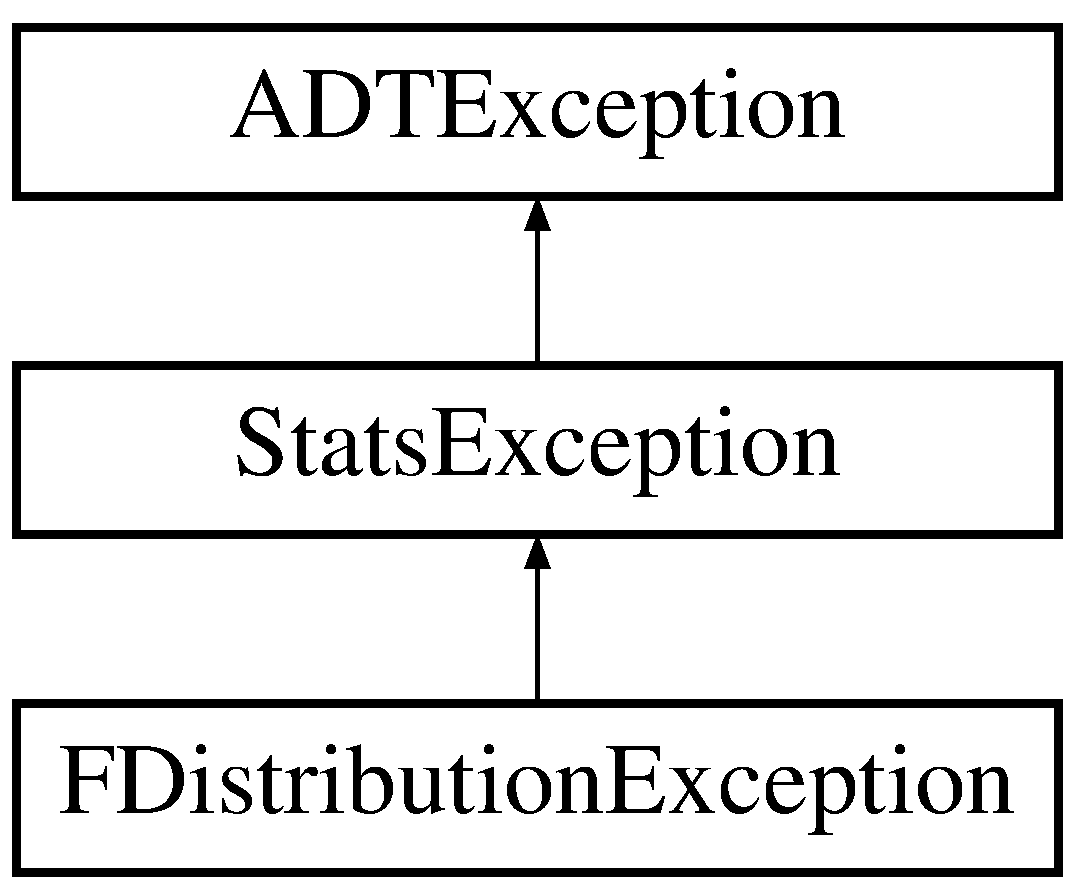
\includegraphics[height=3cm]{classFDistributionException}
\end{center}
\end{figure}


The documentation for this class was generated from the following file:\begin{DoxyCompactItemize}
\item 
engine/utils/\hyperlink{exceptions_8h}{exceptions.h}\end{DoxyCompactItemize}

\hypertarget{classGammaFxnFailureException}{
\section{GammaFxnFailureException Class Reference}
\label{classGammaFxnFailureException}\index{GammaFxnFailureException@{GammaFxnFailureException}}
}


{\ttfamily \#include $<$exceptions.h$>$}

Inheritance diagram for GammaFxnFailureException:\begin{figure}[H]
\begin{center}
\leavevmode
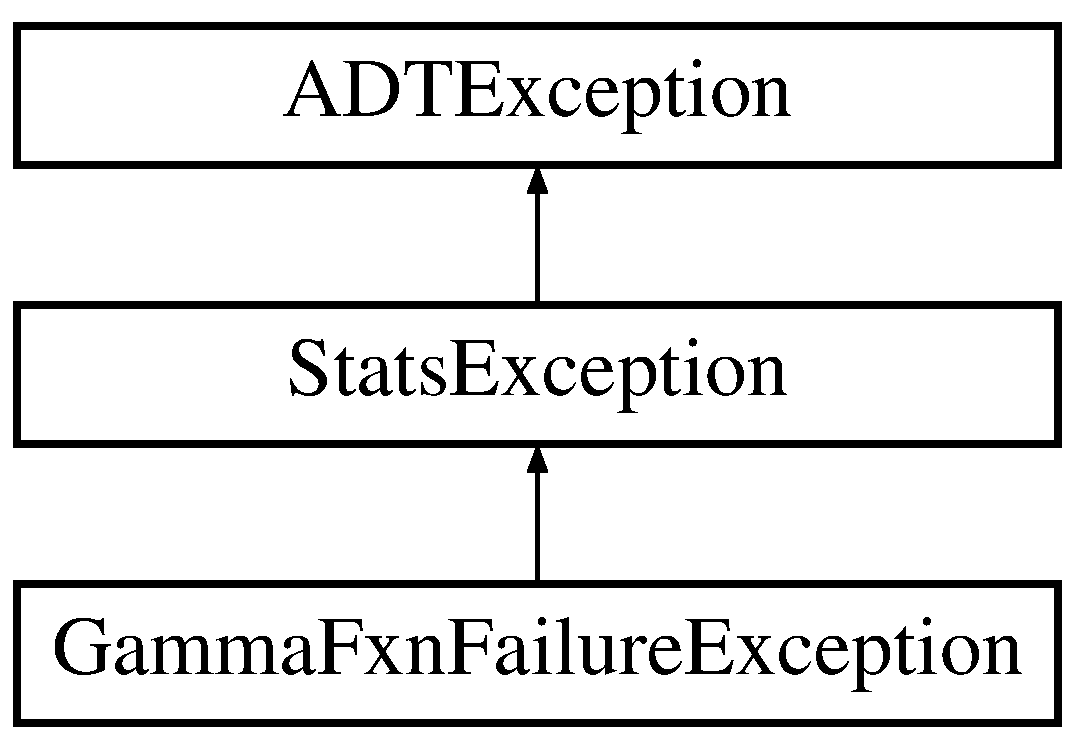
\includegraphics[height=3cm]{classGammaFxnFailureException}
\end{center}
\end{figure}


The documentation for this class was generated from the following file:\begin{DoxyCompactItemize}
\item 
engine/utils/\hyperlink{exceptions_8h}{exceptions.h}\end{DoxyCompactItemize}

\hypertarget{classGenoStats}{
\section{GenoStats Class Reference}
\label{classGenoStats}\index{GenoStats@{GenoStats}}
}


{\ttfamily \#include $<$genostats.hh$>$}

\subsection*{Data Structures}
\begin{DoxyCompactItemize}
\item 
struct {\bfseries errorInformation}
\end{DoxyCompactItemize}
\subsection*{Public Member Functions}
\begin{DoxyCompactItemize}
\item 
\hyperlink{classGenoStats_abda44be89005d401040006d35244931a}{GenoStats} (\hyperlink{classDataAccess}{DataAccess} $\ast$d)
\item 
void \hyperlink{classGenoStats_af40228967a3faba8c13349358f628592}{prepGenoStatsForOutput} (int snp, \hyperlink{structGenoStatsResults}{GenoStatsResults} \&g)
\end{DoxyCompactItemize}


\subsection{Constructor \& Destructor Documentation}
\hypertarget{classGenoStats_abda44be89005d401040006d35244931a}{
\index{GenoStats@{GenoStats}!GenoStats@{GenoStats}}
\index{GenoStats@{GenoStats}!GenoStats@{GenoStats}}
\subsubsection[{GenoStats}]{\setlength{\rightskip}{0pt plus 5cm}GenoStats::GenoStats ({\bf DataAccess} $\ast$ {\em d})}}
\label{classGenoStats_abda44be89005d401040006d35244931a}
Assign the data access.

Also, prep covariate matrix by zero meaning all covariates and preloading. 

\subsection{Member Function Documentation}
\hypertarget{classGenoStats_af40228967a3faba8c13349358f628592}{
\index{GenoStats@{GenoStats}!prepGenoStatsForOutput@{prepGenoStatsForOutput}}
\index{prepGenoStatsForOutput@{prepGenoStatsForOutput}!GenoStats@{GenoStats}}
\subsubsection[{prepGenoStatsForOutput}]{\setlength{\rightskip}{0pt plus 5cm}void GenoStats::prepGenoStatsForOutput (int {\em snp}, \/  {\bf GenoStatsResults} \& {\em g})}}
\label{classGenoStats_af40228967a3faba8c13349358f628592}


The documentation for this class was generated from the following files:\begin{DoxyCompactItemize}
\item 
engine/snpgwa/\hyperlink{genostats_8hh}{genostats.hh}\item 
engine/snpgwa/\hyperlink{genostats_8cpp}{genostats.cpp}\end{DoxyCompactItemize}

\hypertarget{structGenoStatsResults}{
\section{GenoStatsResults Struct Reference}
\label{structGenoStatsResults}\index{GenoStatsResults@{GenoStatsResults}}
}


{\ttfamily \#include $<$snpgwa\_\-out.hh$>$}

\subsection*{Data Fields}
\begin{DoxyCompactItemize}
\item 
double \hyperlink{structGenoStatsResults_a8939e18575bccc8154ee9dd919ce8b90}{twodegTestStat}
\item 
double \hyperlink{structGenoStatsResults_a5de1f45e02308c33f2030392d55a664d}{twodegPVal}
\item 
double \hyperlink{structGenoStatsResults_a26abd8c399efc11a7814df9afd31458c}{domTestStat}
\item 
double \hyperlink{structGenoStatsResults_ad91040dfe4d9a55dc55db1399d0c0d12}{domPVal}
\item 
double \hyperlink{structGenoStatsResults_a8fe0e46c762b32b2b30f8ca36c8e9175}{domOR}
\item 
double \hyperlink{structGenoStatsResults_ab01b69964f41f4dd90a04a09ea14cd8e}{domLCI}
\item 
double \hyperlink{structGenoStatsResults_aef952f406558e7069bc0f5018c19ede3}{domUCI}
\item 
double \hyperlink{structGenoStatsResults_a37f7461f9e3f2985f5e3e31e068efda5}{domSens}
\item 
double \hyperlink{structGenoStatsResults_a3a84dcdd77bcce6a1c0e828508caeb71}{domSpec}
\item 
double \hyperlink{structGenoStatsResults_a317b7bb7d082eb5f277b175a3cd59f26}{domCStat}
\item 
double \hyperlink{structGenoStatsResults_ab488fd76b2583fae71b015f3dc36bcd2}{addTestStat}
\item 
double \hyperlink{structGenoStatsResults_a33e9c29e3701709217756dadcec9e43d}{addPVal}
\item 
double \hyperlink{structGenoStatsResults_a789a736b74e427c069ce2cf4642fe465}{addOR}
\item 
double \hyperlink{structGenoStatsResults_ada26e3e65a779adf42d6598df522f22c}{addLCI}
\item 
double \hyperlink{structGenoStatsResults_a482aec4de6354215ca53d1729bca9093}{addUCI}
\item 
double \hyperlink{structGenoStatsResults_a6ac0807bd05fcf31d48d8192aa095883}{addSensNNRN}
\item 
double \hyperlink{structGenoStatsResults_a7d51f06d687ad181dc9a63fd5fc5b768}{addSpecNNRN}
\item 
double \hyperlink{structGenoStatsResults_a46272ba2d01869dd66808155ebc730d5}{addSensNNRR}
\item 
double \hyperlink{structGenoStatsResults_aa4b0e16cb145bd07a331ca05ae0ab9c4}{addSpecNNRR}
\item 
double \hyperlink{structGenoStatsResults_aa27687e4be8d33aef6258d195c702b53}{addSensNRRR}
\item 
double \hyperlink{structGenoStatsResults_a08e6aba4bebb09fadad7ca931f162d53}{addSpecNRRR}
\item 
double \hyperlink{structGenoStatsResults_ae8171c259ef70ff74c60d4b9bfaa8f66}{addCStat}
\item 
double \hyperlink{structGenoStatsResults_ac0f7db49afdf8540e776a8d38e8629a5}{recTestStat}
\item 
double \hyperlink{structGenoStatsResults_a21a0647a0cfdd5854b384a52a3f71a94}{recPVal}
\item 
double \hyperlink{structGenoStatsResults_a2430df2403f3c1b9a8e05310eaadce90}{recOR}
\item 
double \hyperlink{structGenoStatsResults_a64941b6a97b09760197bd1ce374a9ee5}{recLCI}
\item 
double \hyperlink{structGenoStatsResults_a2aa9578515d50fb8bcef93198c92d63e}{recUCI}
\item 
double \hyperlink{structGenoStatsResults_ac1756c908c9b3c5a303d32c04b250896}{recSens}
\item 
double \hyperlink{structGenoStatsResults_ada57487f856ab09b21ad51bdf339d70c}{recSpec}
\item 
double \hyperlink{structGenoStatsResults_a2014d24446d9eda0ea0ab4dfcdd33df4}{recCStat}
\item 
double \hyperlink{structGenoStatsResults_ac3089d116f118fa8bf7176a8d1a98b89}{lofTestStat}
\item 
double \hyperlink{structGenoStatsResults_ab48fc67c244ac998823af608cc87fc06}{lofPVal}
\end{DoxyCompactItemize}


\subsection{Field Documentation}
\hypertarget{structGenoStatsResults_ae8171c259ef70ff74c60d4b9bfaa8f66}{
\index{GenoStatsResults@{GenoStatsResults}!addCStat@{addCStat}}
\index{addCStat@{addCStat}!GenoStatsResults@{GenoStatsResults}}
\subsubsection[{addCStat}]{\setlength{\rightskip}{0pt plus 5cm}double {\bf GenoStatsResults::addCStat}}}
\label{structGenoStatsResults_ae8171c259ef70ff74c60d4b9bfaa8f66}
\hypertarget{structGenoStatsResults_ada26e3e65a779adf42d6598df522f22c}{
\index{GenoStatsResults@{GenoStatsResults}!addLCI@{addLCI}}
\index{addLCI@{addLCI}!GenoStatsResults@{GenoStatsResults}}
\subsubsection[{addLCI}]{\setlength{\rightskip}{0pt plus 5cm}double {\bf GenoStatsResults::addLCI}}}
\label{structGenoStatsResults_ada26e3e65a779adf42d6598df522f22c}
\hypertarget{structGenoStatsResults_a789a736b74e427c069ce2cf4642fe465}{
\index{GenoStatsResults@{GenoStatsResults}!addOR@{addOR}}
\index{addOR@{addOR}!GenoStatsResults@{GenoStatsResults}}
\subsubsection[{addOR}]{\setlength{\rightskip}{0pt plus 5cm}double {\bf GenoStatsResults::addOR}}}
\label{structGenoStatsResults_a789a736b74e427c069ce2cf4642fe465}
\hypertarget{structGenoStatsResults_a33e9c29e3701709217756dadcec9e43d}{
\index{GenoStatsResults@{GenoStatsResults}!addPVal@{addPVal}}
\index{addPVal@{addPVal}!GenoStatsResults@{GenoStatsResults}}
\subsubsection[{addPVal}]{\setlength{\rightskip}{0pt plus 5cm}double {\bf GenoStatsResults::addPVal}}}
\label{structGenoStatsResults_a33e9c29e3701709217756dadcec9e43d}
\hypertarget{structGenoStatsResults_a6ac0807bd05fcf31d48d8192aa095883}{
\index{GenoStatsResults@{GenoStatsResults}!addSensNNRN@{addSensNNRN}}
\index{addSensNNRN@{addSensNNRN}!GenoStatsResults@{GenoStatsResults}}
\subsubsection[{addSensNNRN}]{\setlength{\rightskip}{0pt plus 5cm}double {\bf GenoStatsResults::addSensNNRN}}}
\label{structGenoStatsResults_a6ac0807bd05fcf31d48d8192aa095883}
\hypertarget{structGenoStatsResults_a46272ba2d01869dd66808155ebc730d5}{
\index{GenoStatsResults@{GenoStatsResults}!addSensNNRR@{addSensNNRR}}
\index{addSensNNRR@{addSensNNRR}!GenoStatsResults@{GenoStatsResults}}
\subsubsection[{addSensNNRR}]{\setlength{\rightskip}{0pt plus 5cm}double {\bf GenoStatsResults::addSensNNRR}}}
\label{structGenoStatsResults_a46272ba2d01869dd66808155ebc730d5}
\hypertarget{structGenoStatsResults_aa27687e4be8d33aef6258d195c702b53}{
\index{GenoStatsResults@{GenoStatsResults}!addSensNRRR@{addSensNRRR}}
\index{addSensNRRR@{addSensNRRR}!GenoStatsResults@{GenoStatsResults}}
\subsubsection[{addSensNRRR}]{\setlength{\rightskip}{0pt plus 5cm}double {\bf GenoStatsResults::addSensNRRR}}}
\label{structGenoStatsResults_aa27687e4be8d33aef6258d195c702b53}
\hypertarget{structGenoStatsResults_a7d51f06d687ad181dc9a63fd5fc5b768}{
\index{GenoStatsResults@{GenoStatsResults}!addSpecNNRN@{addSpecNNRN}}
\index{addSpecNNRN@{addSpecNNRN}!GenoStatsResults@{GenoStatsResults}}
\subsubsection[{addSpecNNRN}]{\setlength{\rightskip}{0pt plus 5cm}double {\bf GenoStatsResults::addSpecNNRN}}}
\label{structGenoStatsResults_a7d51f06d687ad181dc9a63fd5fc5b768}
\hypertarget{structGenoStatsResults_aa4b0e16cb145bd07a331ca05ae0ab9c4}{
\index{GenoStatsResults@{GenoStatsResults}!addSpecNNRR@{addSpecNNRR}}
\index{addSpecNNRR@{addSpecNNRR}!GenoStatsResults@{GenoStatsResults}}
\subsubsection[{addSpecNNRR}]{\setlength{\rightskip}{0pt plus 5cm}double {\bf GenoStatsResults::addSpecNNRR}}}
\label{structGenoStatsResults_aa4b0e16cb145bd07a331ca05ae0ab9c4}
\hypertarget{structGenoStatsResults_a08e6aba4bebb09fadad7ca931f162d53}{
\index{GenoStatsResults@{GenoStatsResults}!addSpecNRRR@{addSpecNRRR}}
\index{addSpecNRRR@{addSpecNRRR}!GenoStatsResults@{GenoStatsResults}}
\subsubsection[{addSpecNRRR}]{\setlength{\rightskip}{0pt plus 5cm}double {\bf GenoStatsResults::addSpecNRRR}}}
\label{structGenoStatsResults_a08e6aba4bebb09fadad7ca931f162d53}
\hypertarget{structGenoStatsResults_ab488fd76b2583fae71b015f3dc36bcd2}{
\index{GenoStatsResults@{GenoStatsResults}!addTestStat@{addTestStat}}
\index{addTestStat@{addTestStat}!GenoStatsResults@{GenoStatsResults}}
\subsubsection[{addTestStat}]{\setlength{\rightskip}{0pt plus 5cm}double {\bf GenoStatsResults::addTestStat}}}
\label{structGenoStatsResults_ab488fd76b2583fae71b015f3dc36bcd2}
\hypertarget{structGenoStatsResults_a482aec4de6354215ca53d1729bca9093}{
\index{GenoStatsResults@{GenoStatsResults}!addUCI@{addUCI}}
\index{addUCI@{addUCI}!GenoStatsResults@{GenoStatsResults}}
\subsubsection[{addUCI}]{\setlength{\rightskip}{0pt plus 5cm}double {\bf GenoStatsResults::addUCI}}}
\label{structGenoStatsResults_a482aec4de6354215ca53d1729bca9093}
\hypertarget{structGenoStatsResults_a317b7bb7d082eb5f277b175a3cd59f26}{
\index{GenoStatsResults@{GenoStatsResults}!domCStat@{domCStat}}
\index{domCStat@{domCStat}!GenoStatsResults@{GenoStatsResults}}
\subsubsection[{domCStat}]{\setlength{\rightskip}{0pt plus 5cm}double {\bf GenoStatsResults::domCStat}}}
\label{structGenoStatsResults_a317b7bb7d082eb5f277b175a3cd59f26}
\hypertarget{structGenoStatsResults_ab01b69964f41f4dd90a04a09ea14cd8e}{
\index{GenoStatsResults@{GenoStatsResults}!domLCI@{domLCI}}
\index{domLCI@{domLCI}!GenoStatsResults@{GenoStatsResults}}
\subsubsection[{domLCI}]{\setlength{\rightskip}{0pt plus 5cm}double {\bf GenoStatsResults::domLCI}}}
\label{structGenoStatsResults_ab01b69964f41f4dd90a04a09ea14cd8e}
\hypertarget{structGenoStatsResults_a8fe0e46c762b32b2b30f8ca36c8e9175}{
\index{GenoStatsResults@{GenoStatsResults}!domOR@{domOR}}
\index{domOR@{domOR}!GenoStatsResults@{GenoStatsResults}}
\subsubsection[{domOR}]{\setlength{\rightskip}{0pt plus 5cm}double {\bf GenoStatsResults::domOR}}}
\label{structGenoStatsResults_a8fe0e46c762b32b2b30f8ca36c8e9175}
\hypertarget{structGenoStatsResults_ad91040dfe4d9a55dc55db1399d0c0d12}{
\index{GenoStatsResults@{GenoStatsResults}!domPVal@{domPVal}}
\index{domPVal@{domPVal}!GenoStatsResults@{GenoStatsResults}}
\subsubsection[{domPVal}]{\setlength{\rightskip}{0pt plus 5cm}double {\bf GenoStatsResults::domPVal}}}
\label{structGenoStatsResults_ad91040dfe4d9a55dc55db1399d0c0d12}
\hypertarget{structGenoStatsResults_a37f7461f9e3f2985f5e3e31e068efda5}{
\index{GenoStatsResults@{GenoStatsResults}!domSens@{domSens}}
\index{domSens@{domSens}!GenoStatsResults@{GenoStatsResults}}
\subsubsection[{domSens}]{\setlength{\rightskip}{0pt plus 5cm}double {\bf GenoStatsResults::domSens}}}
\label{structGenoStatsResults_a37f7461f9e3f2985f5e3e31e068efda5}
\hypertarget{structGenoStatsResults_a3a84dcdd77bcce6a1c0e828508caeb71}{
\index{GenoStatsResults@{GenoStatsResults}!domSpec@{domSpec}}
\index{domSpec@{domSpec}!GenoStatsResults@{GenoStatsResults}}
\subsubsection[{domSpec}]{\setlength{\rightskip}{0pt plus 5cm}double {\bf GenoStatsResults::domSpec}}}
\label{structGenoStatsResults_a3a84dcdd77bcce6a1c0e828508caeb71}
\hypertarget{structGenoStatsResults_a26abd8c399efc11a7814df9afd31458c}{
\index{GenoStatsResults@{GenoStatsResults}!domTestStat@{domTestStat}}
\index{domTestStat@{domTestStat}!GenoStatsResults@{GenoStatsResults}}
\subsubsection[{domTestStat}]{\setlength{\rightskip}{0pt plus 5cm}double {\bf GenoStatsResults::domTestStat}}}
\label{structGenoStatsResults_a26abd8c399efc11a7814df9afd31458c}
\hypertarget{structGenoStatsResults_aef952f406558e7069bc0f5018c19ede3}{
\index{GenoStatsResults@{GenoStatsResults}!domUCI@{domUCI}}
\index{domUCI@{domUCI}!GenoStatsResults@{GenoStatsResults}}
\subsubsection[{domUCI}]{\setlength{\rightskip}{0pt plus 5cm}double {\bf GenoStatsResults::domUCI}}}
\label{structGenoStatsResults_aef952f406558e7069bc0f5018c19ede3}
\hypertarget{structGenoStatsResults_ab48fc67c244ac998823af608cc87fc06}{
\index{GenoStatsResults@{GenoStatsResults}!lofPVal@{lofPVal}}
\index{lofPVal@{lofPVal}!GenoStatsResults@{GenoStatsResults}}
\subsubsection[{lofPVal}]{\setlength{\rightskip}{0pt plus 5cm}double {\bf GenoStatsResults::lofPVal}}}
\label{structGenoStatsResults_ab48fc67c244ac998823af608cc87fc06}
\hypertarget{structGenoStatsResults_ac3089d116f118fa8bf7176a8d1a98b89}{
\index{GenoStatsResults@{GenoStatsResults}!lofTestStat@{lofTestStat}}
\index{lofTestStat@{lofTestStat}!GenoStatsResults@{GenoStatsResults}}
\subsubsection[{lofTestStat}]{\setlength{\rightskip}{0pt plus 5cm}double {\bf GenoStatsResults::lofTestStat}}}
\label{structGenoStatsResults_ac3089d116f118fa8bf7176a8d1a98b89}
\hypertarget{structGenoStatsResults_a2014d24446d9eda0ea0ab4dfcdd33df4}{
\index{GenoStatsResults@{GenoStatsResults}!recCStat@{recCStat}}
\index{recCStat@{recCStat}!GenoStatsResults@{GenoStatsResults}}
\subsubsection[{recCStat}]{\setlength{\rightskip}{0pt plus 5cm}double {\bf GenoStatsResults::recCStat}}}
\label{structGenoStatsResults_a2014d24446d9eda0ea0ab4dfcdd33df4}
\hypertarget{structGenoStatsResults_a64941b6a97b09760197bd1ce374a9ee5}{
\index{GenoStatsResults@{GenoStatsResults}!recLCI@{recLCI}}
\index{recLCI@{recLCI}!GenoStatsResults@{GenoStatsResults}}
\subsubsection[{recLCI}]{\setlength{\rightskip}{0pt plus 5cm}double {\bf GenoStatsResults::recLCI}}}
\label{structGenoStatsResults_a64941b6a97b09760197bd1ce374a9ee5}
\hypertarget{structGenoStatsResults_a2430df2403f3c1b9a8e05310eaadce90}{
\index{GenoStatsResults@{GenoStatsResults}!recOR@{recOR}}
\index{recOR@{recOR}!GenoStatsResults@{GenoStatsResults}}
\subsubsection[{recOR}]{\setlength{\rightskip}{0pt plus 5cm}double {\bf GenoStatsResults::recOR}}}
\label{structGenoStatsResults_a2430df2403f3c1b9a8e05310eaadce90}
\hypertarget{structGenoStatsResults_a21a0647a0cfdd5854b384a52a3f71a94}{
\index{GenoStatsResults@{GenoStatsResults}!recPVal@{recPVal}}
\index{recPVal@{recPVal}!GenoStatsResults@{GenoStatsResults}}
\subsubsection[{recPVal}]{\setlength{\rightskip}{0pt plus 5cm}double {\bf GenoStatsResults::recPVal}}}
\label{structGenoStatsResults_a21a0647a0cfdd5854b384a52a3f71a94}
\hypertarget{structGenoStatsResults_ac1756c908c9b3c5a303d32c04b250896}{
\index{GenoStatsResults@{GenoStatsResults}!recSens@{recSens}}
\index{recSens@{recSens}!GenoStatsResults@{GenoStatsResults}}
\subsubsection[{recSens}]{\setlength{\rightskip}{0pt plus 5cm}double {\bf GenoStatsResults::recSens}}}
\label{structGenoStatsResults_ac1756c908c9b3c5a303d32c04b250896}
\hypertarget{structGenoStatsResults_ada57487f856ab09b21ad51bdf339d70c}{
\index{GenoStatsResults@{GenoStatsResults}!recSpec@{recSpec}}
\index{recSpec@{recSpec}!GenoStatsResults@{GenoStatsResults}}
\subsubsection[{recSpec}]{\setlength{\rightskip}{0pt plus 5cm}double {\bf GenoStatsResults::recSpec}}}
\label{structGenoStatsResults_ada57487f856ab09b21ad51bdf339d70c}
\hypertarget{structGenoStatsResults_ac0f7db49afdf8540e776a8d38e8629a5}{
\index{GenoStatsResults@{GenoStatsResults}!recTestStat@{recTestStat}}
\index{recTestStat@{recTestStat}!GenoStatsResults@{GenoStatsResults}}
\subsubsection[{recTestStat}]{\setlength{\rightskip}{0pt plus 5cm}double {\bf GenoStatsResults::recTestStat}}}
\label{structGenoStatsResults_ac0f7db49afdf8540e776a8d38e8629a5}
\hypertarget{structGenoStatsResults_a2aa9578515d50fb8bcef93198c92d63e}{
\index{GenoStatsResults@{GenoStatsResults}!recUCI@{recUCI}}
\index{recUCI@{recUCI}!GenoStatsResults@{GenoStatsResults}}
\subsubsection[{recUCI}]{\setlength{\rightskip}{0pt plus 5cm}double {\bf GenoStatsResults::recUCI}}}
\label{structGenoStatsResults_a2aa9578515d50fb8bcef93198c92d63e}
\hypertarget{structGenoStatsResults_a5de1f45e02308c33f2030392d55a664d}{
\index{GenoStatsResults@{GenoStatsResults}!twodegPVal@{twodegPVal}}
\index{twodegPVal@{twodegPVal}!GenoStatsResults@{GenoStatsResults}}
\subsubsection[{twodegPVal}]{\setlength{\rightskip}{0pt plus 5cm}double {\bf GenoStatsResults::twodegPVal}}}
\label{structGenoStatsResults_a5de1f45e02308c33f2030392d55a664d}
\hypertarget{structGenoStatsResults_a8939e18575bccc8154ee9dd919ce8b90}{
\index{GenoStatsResults@{GenoStatsResults}!twodegTestStat@{twodegTestStat}}
\index{twodegTestStat@{twodegTestStat}!GenoStatsResults@{GenoStatsResults}}
\subsubsection[{twodegTestStat}]{\setlength{\rightskip}{0pt plus 5cm}double {\bf GenoStatsResults::twodegTestStat}}}
\label{structGenoStatsResults_a8939e18575bccc8154ee9dd919ce8b90}


The documentation for this struct was generated from the following file:\begin{DoxyCompactItemize}
\item 
engine/output/\hyperlink{snpgwa__out_8hh}{snpgwa\_\-out.hh}\end{DoxyCompactItemize}

\hypertarget{classHaploStats}{
\section{HaploStats Class Reference}
\label{classHaploStats}\index{HaploStats@{HaploStats}}
}


{\ttfamily \#include $<$haplostats.hh$>$}

\subsection*{Public Member Functions}
\begin{DoxyCompactItemize}
\item 
\hyperlink{classHaploStats_ada2d93862b794d80fe0903410689234e}{HaploStats} (\hyperlink{classDataAccess}{DataAccess} $\ast$)
\item 
void \hyperlink{classHaploStats_a2e17c8ccd68b20b4a2cb20e91025c13e}{prepHaploStatsForOutput} (int, \hyperlink{structHaploStatsResults}{HaploStatsResults} \&)
\item 
void \hyperlink{classHaploStats_a5f5c2445d79a7913381ff0ac5d8f53d4}{setHaploThresh} (int k)
\end{DoxyCompactItemize}
\subsection*{Protected Member Functions}
\begin{DoxyCompactItemize}
\item 
void \hyperlink{classHaploStats_ae7c212db625f88424070abcc364ed89f}{calculateAllelic} (int)
\item 
void \hyperlink{classHaploStats_a4eb4a1554f92c356d3d6bcb3f15a4daf}{calculateTwoMarker} (int, int)
\item 
void \hyperlink{classHaploStats_af2525446b1f48c377adeffd328c53cba}{calculateThreeMarker} (int, int, int)
\item 
double \hyperlink{classHaploStats_a8f9a2f53316b3e76f350dbd68589ccb0}{computeGlobalZaykinStatisic} (\hyperlink{classEM}{EM} \&em, int size, double \&testStat, int \&degFreedom)
\item 
double \hyperlink{classHaploStats_a25999dcaac8dabc7a4c10a0992db61fb}{computeGlobalZaykinStatisic} (\hyperlink{classEM}{EM} \&em, int size, double \&testStat, int \&degFreedom, const vector$<$ double $>$ \&phenotype, const vector$<$ vector$<$ double $>$ $>$ \&cov, int snp)
\end{DoxyCompactItemize}
\subsection*{Static Protected Member Functions}
\begin{DoxyCompactItemize}
\item 
static double \hyperlink{classHaploStats_ad2719f7191d458bf72cf117b0d581aaa}{EPS} ()
\begin{DoxyCompactList}\small\item\em Used by \hyperlink{classZaykin}{Zaykin}. Passed in at start. \item\end{DoxyCompactList}\end{DoxyCompactItemize}
\subsection*{Protected Attributes}
\begin{DoxyCompactItemize}
\item 
\hyperlink{classDataAccess}{DataAccess} $\ast$ \hyperlink{classHaploStats_aae230c13a34d75fe7e07ab7ae75b2c6d}{data}
\item 
double \hyperlink{classHaploStats_ac19e1b8dcc610e73969faad69b27ccc6}{allelicPval}
\item 
double \hyperlink{classHaploStats_a4fe152dc428bff18ec9d04254834eff1}{allelicChiSq}
\item 
int \hyperlink{classHaploStats_a839271fb722730e8b45127525c471fe6}{allelicDF}
\item 
double \hyperlink{classHaploStats_ae385ebf05af0fa4d0199f4ffa8fd6c74}{twoMarkerPval}
\item 
double \hyperlink{classHaploStats_ae09deb6ca71b310c0c8362b0c92bd116}{twoMarkerChiS}
\item 
int \hyperlink{classHaploStats_a9cfc39f1d2348301cad42b3a4b600229}{twoMarkerDF}
\item 
vector$<$ double $>$ \hyperlink{classHaploStats_ac65cb68586d5102e6b771b5d2cca24eb}{twoMarkerCaseHapFreq}
\item 
vector$<$ double $>$ \hyperlink{classHaploStats_a68d73b06d601fa5809b051f8458a2a23}{twoMarkerCntrlHapFreq}
\item 
vector$<$ double $>$ \hyperlink{classHaploStats_a0a4928ebe077029a82a13fcdb10910c7}{twoMarkerCmbdHapFreq}
\item 
double \hyperlink{classHaploStats_aaaff3d8ec32e831c25296fca296b3f25}{threeMarkerPval}
\item 
double \hyperlink{classHaploStats_a7146d3781769f3c30c353ebc6552bf8c}{threeMarkerChiS}
\item 
int \hyperlink{classHaploStats_a88b45a1784a3af46f1727325f1520300}{threeMarkerDF}
\item 
vector$<$ double $>$ \hyperlink{classHaploStats_ab9fe88dff2fea23a2d76ab656f5a22ec}{threeMarkerCaseHapFreq}
\item 
vector$<$ double $>$ \hyperlink{classHaploStats_aeabf9d28af93060be4d3b7a06a36684c}{threeMarkerCntrlHapFreq}
\item 
vector$<$ double $>$ \hyperlink{classHaploStats_ae4aa675ce11d88b43564c7ca54cc9f3f}{threeMarkerCmbdHapFreq}
\item 
int \hyperlink{classHaploStats_a856613cafb08e96a0fc267ab3a5482fc}{haploThresh}
\end{DoxyCompactItemize}


\subsection{Constructor \& Destructor Documentation}
\hypertarget{classHaploStats_ada2d93862b794d80fe0903410689234e}{
\index{HaploStats@{HaploStats}!HaploStats@{HaploStats}}
\index{HaploStats@{HaploStats}!HaploStats@{HaploStats}}
\subsubsection[{HaploStats}]{\setlength{\rightskip}{0pt plus 5cm}HaploStats::HaploStats ({\bf DataAccess} $\ast$ {\em d})}}
\label{classHaploStats_ada2d93862b794d80fe0903410689234e}


\subsection{Member Function Documentation}
\hypertarget{classHaploStats_ae7c212db625f88424070abcc364ed89f}{
\index{HaploStats@{HaploStats}!calculateAllelic@{calculateAllelic}}
\index{calculateAllelic@{calculateAllelic}!HaploStats@{HaploStats}}
\subsubsection[{calculateAllelic}]{\setlength{\rightskip}{0pt plus 5cm}void HaploStats::calculateAllelic (int {\em snp})\hspace{0.3cm}{\ttfamily  \mbox{[}protected\mbox{]}}}}
\label{classHaploStats_ae7c212db625f88424070abcc364ed89f}
Calculate allelic test. This can be conceived as a single SNP haplotype test where all of hte haplotpyes are known with probability one. It leverages the code built for larger hapltoypes, but \hyperlink{classEM}{EM} is never called. \hypertarget{classHaploStats_af2525446b1f48c377adeffd328c53cba}{
\index{HaploStats@{HaploStats}!calculateThreeMarker@{calculateThreeMarker}}
\index{calculateThreeMarker@{calculateThreeMarker}!HaploStats@{HaploStats}}
\subsubsection[{calculateThreeMarker}]{\setlength{\rightskip}{0pt plus 5cm}void HaploStats::calculateThreeMarker (int {\em s1}, \/  int {\em s2}, \/  int {\em s3})\hspace{0.3cm}{\ttfamily  \mbox{[}protected\mbox{]}}}}
\label{classHaploStats_af2525446b1f48c377adeffd328c53cba}
Calculate the three marker haplotype test.

Steps: 1) Prep and run the \hyperlink{classEM}{EM} algorithm for cases and for controls. 2) Calculate haplotypic associatoin \hypertarget{classHaploStats_a4eb4a1554f92c356d3d6bcb3f15a4daf}{
\index{HaploStats@{HaploStats}!calculateTwoMarker@{calculateTwoMarker}}
\index{calculateTwoMarker@{calculateTwoMarker}!HaploStats@{HaploStats}}
\subsubsection[{calculateTwoMarker}]{\setlength{\rightskip}{0pt plus 5cm}void HaploStats::calculateTwoMarker (int {\em s1}, \/  int {\em s2})\hspace{0.3cm}{\ttfamily  \mbox{[}protected\mbox{]}}}}
\label{classHaploStats_a4eb4a1554f92c356d3d6bcb3f15a4daf}
Calculate the two marker haplotype test.

Steps: 1) Prep and run the \hyperlink{classEM}{EM} algorithm for cases and for controls. 2) Calculate haplotypic associatoin \hypertarget{classHaploStats_a25999dcaac8dabc7a4c10a0992db61fb}{
\index{HaploStats@{HaploStats}!computeGlobalZaykinStatisic@{computeGlobalZaykinStatisic}}
\index{computeGlobalZaykinStatisic@{computeGlobalZaykinStatisic}!HaploStats@{HaploStats}}
\subsubsection[{computeGlobalZaykinStatisic}]{\setlength{\rightskip}{0pt plus 5cm}double HaploStats::computeGlobalZaykinStatisic ({\bf EM} \& {\em em}, \/  int {\em size}, \/  double \& {\em testStat}, \/  int \& {\em degFreedom}, \/  const vector$<$ double $>$ \& {\em phenotype}, \/  const vector$<$ vector$<$ double $>$ $>$ \& {\em cov}, \/  int {\em snp})\hspace{0.3cm}{\ttfamily  \mbox{[}protected\mbox{]}}}}
\label{classHaploStats_a25999dcaac8dabc7a4c10a0992db61fb}
\hypertarget{classHaploStats_a8f9a2f53316b3e76f350dbd68589ccb0}{
\index{HaploStats@{HaploStats}!computeGlobalZaykinStatisic@{computeGlobalZaykinStatisic}}
\index{computeGlobalZaykinStatisic@{computeGlobalZaykinStatisic}!HaploStats@{HaploStats}}
\subsubsection[{computeGlobalZaykinStatisic}]{\setlength{\rightskip}{0pt plus 5cm}double HaploStats::computeGlobalZaykinStatisic ({\bf EM} \& {\em em}, \/  int {\em size}, \/  double \& {\em testStat}, \/  int \& {\em degFreedom})\hspace{0.3cm}{\ttfamily  \mbox{[}protected\mbox{]}}}}
\label{classHaploStats_a8f9a2f53316b3e76f350dbd68589ccb0}
\hypertarget{classHaploStats_ad2719f7191d458bf72cf117b0d581aaa}{
\index{HaploStats@{HaploStats}!EPS@{EPS}}
\index{EPS@{EPS}!HaploStats@{HaploStats}}
\subsubsection[{EPS}]{\setlength{\rightskip}{0pt plus 5cm}static double HaploStats::EPS ()\hspace{0.3cm}{\ttfamily  \mbox{[}inline, static, protected\mbox{]}}}}
\label{classHaploStats_ad2719f7191d458bf72cf117b0d581aaa}


Used by \hyperlink{classZaykin}{Zaykin}. Passed in at start. 

\hypertarget{classHaploStats_a2e17c8ccd68b20b4a2cb20e91025c13e}{
\index{HaploStats@{HaploStats}!prepHaploStatsForOutput@{prepHaploStatsForOutput}}
\index{prepHaploStatsForOutput@{prepHaploStatsForOutput}!HaploStats@{HaploStats}}
\subsubsection[{prepHaploStatsForOutput}]{\setlength{\rightskip}{0pt plus 5cm}void HaploStats::prepHaploStatsForOutput (int {\em snp}, \/  {\bf HaploStatsResults} \& {\em res})}}
\label{classHaploStats_a2e17c8ccd68b20b4a2cb20e91025c13e}
\hypertarget{classHaploStats_a5f5c2445d79a7913381ff0ac5d8f53d4}{
\index{HaploStats@{HaploStats}!setHaploThresh@{setHaploThresh}}
\index{setHaploThresh@{setHaploThresh}!HaploStats@{HaploStats}}
\subsubsection[{setHaploThresh}]{\setlength{\rightskip}{0pt plus 5cm}void HaploStats::setHaploThresh (int {\em k})\hspace{0.3cm}{\ttfamily  \mbox{[}inline\mbox{]}}}}
\label{classHaploStats_a5f5c2445d79a7913381ff0ac5d8f53d4}


\subsection{Field Documentation}
\hypertarget{classHaploStats_a4fe152dc428bff18ec9d04254834eff1}{
\index{HaploStats@{HaploStats}!allelicChiSq@{allelicChiSq}}
\index{allelicChiSq@{allelicChiSq}!HaploStats@{HaploStats}}
\subsubsection[{allelicChiSq}]{\setlength{\rightskip}{0pt plus 5cm}double {\bf HaploStats::allelicChiSq}\hspace{0.3cm}{\ttfamily  \mbox{[}protected\mbox{]}}}}
\label{classHaploStats_a4fe152dc428bff18ec9d04254834eff1}
\hypertarget{classHaploStats_a839271fb722730e8b45127525c471fe6}{
\index{HaploStats@{HaploStats}!allelicDF@{allelicDF}}
\index{allelicDF@{allelicDF}!HaploStats@{HaploStats}}
\subsubsection[{allelicDF}]{\setlength{\rightskip}{0pt plus 5cm}int {\bf HaploStats::allelicDF}\hspace{0.3cm}{\ttfamily  \mbox{[}protected\mbox{]}}}}
\label{classHaploStats_a839271fb722730e8b45127525c471fe6}
\hypertarget{classHaploStats_ac19e1b8dcc610e73969faad69b27ccc6}{
\index{HaploStats@{HaploStats}!allelicPval@{allelicPval}}
\index{allelicPval@{allelicPval}!HaploStats@{HaploStats}}
\subsubsection[{allelicPval}]{\setlength{\rightskip}{0pt plus 5cm}double {\bf HaploStats::allelicPval}\hspace{0.3cm}{\ttfamily  \mbox{[}protected\mbox{]}}}}
\label{classHaploStats_ac19e1b8dcc610e73969faad69b27ccc6}
\hypertarget{classHaploStats_aae230c13a34d75fe7e07ab7ae75b2c6d}{
\index{HaploStats@{HaploStats}!data@{data}}
\index{data@{data}!HaploStats@{HaploStats}}
\subsubsection[{data}]{\setlength{\rightskip}{0pt plus 5cm}{\bf DataAccess}$\ast$ {\bf HaploStats::data}\hspace{0.3cm}{\ttfamily  \mbox{[}protected\mbox{]}}}}
\label{classHaploStats_aae230c13a34d75fe7e07ab7ae75b2c6d}
\hypertarget{classHaploStats_a856613cafb08e96a0fc267ab3a5482fc}{
\index{HaploStats@{HaploStats}!haploThresh@{haploThresh}}
\index{haploThresh@{haploThresh}!HaploStats@{HaploStats}}
\subsubsection[{haploThresh}]{\setlength{\rightskip}{0pt plus 5cm}int {\bf HaploStats::haploThresh}\hspace{0.3cm}{\ttfamily  \mbox{[}protected\mbox{]}}}}
\label{classHaploStats_a856613cafb08e96a0fc267ab3a5482fc}
\hypertarget{classHaploStats_ab9fe88dff2fea23a2d76ab656f5a22ec}{
\index{HaploStats@{HaploStats}!threeMarkerCaseHapFreq@{threeMarkerCaseHapFreq}}
\index{threeMarkerCaseHapFreq@{threeMarkerCaseHapFreq}!HaploStats@{HaploStats}}
\subsubsection[{threeMarkerCaseHapFreq}]{\setlength{\rightskip}{0pt plus 5cm}vector$<$double$>$ {\bf HaploStats::threeMarkerCaseHapFreq}\hspace{0.3cm}{\ttfamily  \mbox{[}protected\mbox{]}}}}
\label{classHaploStats_ab9fe88dff2fea23a2d76ab656f5a22ec}
\hypertarget{classHaploStats_a7146d3781769f3c30c353ebc6552bf8c}{
\index{HaploStats@{HaploStats}!threeMarkerChiS@{threeMarkerChiS}}
\index{threeMarkerChiS@{threeMarkerChiS}!HaploStats@{HaploStats}}
\subsubsection[{threeMarkerChiS}]{\setlength{\rightskip}{0pt plus 5cm}double {\bf HaploStats::threeMarkerChiS}\hspace{0.3cm}{\ttfamily  \mbox{[}protected\mbox{]}}}}
\label{classHaploStats_a7146d3781769f3c30c353ebc6552bf8c}
\hypertarget{classHaploStats_ae4aa675ce11d88b43564c7ca54cc9f3f}{
\index{HaploStats@{HaploStats}!threeMarkerCmbdHapFreq@{threeMarkerCmbdHapFreq}}
\index{threeMarkerCmbdHapFreq@{threeMarkerCmbdHapFreq}!HaploStats@{HaploStats}}
\subsubsection[{threeMarkerCmbdHapFreq}]{\setlength{\rightskip}{0pt plus 5cm}vector$<$double$>$ {\bf HaploStats::threeMarkerCmbdHapFreq}\hspace{0.3cm}{\ttfamily  \mbox{[}protected\mbox{]}}}}
\label{classHaploStats_ae4aa675ce11d88b43564c7ca54cc9f3f}
\hypertarget{classHaploStats_aeabf9d28af93060be4d3b7a06a36684c}{
\index{HaploStats@{HaploStats}!threeMarkerCntrlHapFreq@{threeMarkerCntrlHapFreq}}
\index{threeMarkerCntrlHapFreq@{threeMarkerCntrlHapFreq}!HaploStats@{HaploStats}}
\subsubsection[{threeMarkerCntrlHapFreq}]{\setlength{\rightskip}{0pt plus 5cm}vector$<$double$>$ {\bf HaploStats::threeMarkerCntrlHapFreq}\hspace{0.3cm}{\ttfamily  \mbox{[}protected\mbox{]}}}}
\label{classHaploStats_aeabf9d28af93060be4d3b7a06a36684c}
\hypertarget{classHaploStats_a88b45a1784a3af46f1727325f1520300}{
\index{HaploStats@{HaploStats}!threeMarkerDF@{threeMarkerDF}}
\index{threeMarkerDF@{threeMarkerDF}!HaploStats@{HaploStats}}
\subsubsection[{threeMarkerDF}]{\setlength{\rightskip}{0pt plus 5cm}int {\bf HaploStats::threeMarkerDF}\hspace{0.3cm}{\ttfamily  \mbox{[}protected\mbox{]}}}}
\label{classHaploStats_a88b45a1784a3af46f1727325f1520300}
\hypertarget{classHaploStats_aaaff3d8ec32e831c25296fca296b3f25}{
\index{HaploStats@{HaploStats}!threeMarkerPval@{threeMarkerPval}}
\index{threeMarkerPval@{threeMarkerPval}!HaploStats@{HaploStats}}
\subsubsection[{threeMarkerPval}]{\setlength{\rightskip}{0pt plus 5cm}double {\bf HaploStats::threeMarkerPval}\hspace{0.3cm}{\ttfamily  \mbox{[}protected\mbox{]}}}}
\label{classHaploStats_aaaff3d8ec32e831c25296fca296b3f25}
\hypertarget{classHaploStats_ac65cb68586d5102e6b771b5d2cca24eb}{
\index{HaploStats@{HaploStats}!twoMarkerCaseHapFreq@{twoMarkerCaseHapFreq}}
\index{twoMarkerCaseHapFreq@{twoMarkerCaseHapFreq}!HaploStats@{HaploStats}}
\subsubsection[{twoMarkerCaseHapFreq}]{\setlength{\rightskip}{0pt plus 5cm}vector$<$double$>$ {\bf HaploStats::twoMarkerCaseHapFreq}\hspace{0.3cm}{\ttfamily  \mbox{[}protected\mbox{]}}}}
\label{classHaploStats_ac65cb68586d5102e6b771b5d2cca24eb}
\hypertarget{classHaploStats_ae09deb6ca71b310c0c8362b0c92bd116}{
\index{HaploStats@{HaploStats}!twoMarkerChiS@{twoMarkerChiS}}
\index{twoMarkerChiS@{twoMarkerChiS}!HaploStats@{HaploStats}}
\subsubsection[{twoMarkerChiS}]{\setlength{\rightskip}{0pt plus 5cm}double {\bf HaploStats::twoMarkerChiS}\hspace{0.3cm}{\ttfamily  \mbox{[}protected\mbox{]}}}}
\label{classHaploStats_ae09deb6ca71b310c0c8362b0c92bd116}
\hypertarget{classHaploStats_a0a4928ebe077029a82a13fcdb10910c7}{
\index{HaploStats@{HaploStats}!twoMarkerCmbdHapFreq@{twoMarkerCmbdHapFreq}}
\index{twoMarkerCmbdHapFreq@{twoMarkerCmbdHapFreq}!HaploStats@{HaploStats}}
\subsubsection[{twoMarkerCmbdHapFreq}]{\setlength{\rightskip}{0pt plus 5cm}vector$<$double$>$ {\bf HaploStats::twoMarkerCmbdHapFreq}\hspace{0.3cm}{\ttfamily  \mbox{[}protected\mbox{]}}}}
\label{classHaploStats_a0a4928ebe077029a82a13fcdb10910c7}
\hypertarget{classHaploStats_a68d73b06d601fa5809b051f8458a2a23}{
\index{HaploStats@{HaploStats}!twoMarkerCntrlHapFreq@{twoMarkerCntrlHapFreq}}
\index{twoMarkerCntrlHapFreq@{twoMarkerCntrlHapFreq}!HaploStats@{HaploStats}}
\subsubsection[{twoMarkerCntrlHapFreq}]{\setlength{\rightskip}{0pt plus 5cm}vector$<$double$>$ {\bf HaploStats::twoMarkerCntrlHapFreq}\hspace{0.3cm}{\ttfamily  \mbox{[}protected\mbox{]}}}}
\label{classHaploStats_a68d73b06d601fa5809b051f8458a2a23}
\hypertarget{classHaploStats_a9cfc39f1d2348301cad42b3a4b600229}{
\index{HaploStats@{HaploStats}!twoMarkerDF@{twoMarkerDF}}
\index{twoMarkerDF@{twoMarkerDF}!HaploStats@{HaploStats}}
\subsubsection[{twoMarkerDF}]{\setlength{\rightskip}{0pt plus 5cm}int {\bf HaploStats::twoMarkerDF}\hspace{0.3cm}{\ttfamily  \mbox{[}protected\mbox{]}}}}
\label{classHaploStats_a9cfc39f1d2348301cad42b3a4b600229}
\hypertarget{classHaploStats_ae385ebf05af0fa4d0199f4ffa8fd6c74}{
\index{HaploStats@{HaploStats}!twoMarkerPval@{twoMarkerPval}}
\index{twoMarkerPval@{twoMarkerPval}!HaploStats@{HaploStats}}
\subsubsection[{twoMarkerPval}]{\setlength{\rightskip}{0pt plus 5cm}double {\bf HaploStats::twoMarkerPval}\hspace{0.3cm}{\ttfamily  \mbox{[}protected\mbox{]}}}}
\label{classHaploStats_ae385ebf05af0fa4d0199f4ffa8fd6c74}


The documentation for this class was generated from the following files:\begin{DoxyCompactItemize}
\item 
engine/snpgwa/\hyperlink{haplostats_8hh}{haplostats.hh}\item 
engine/snpgwa/\hyperlink{haplostats_8cpp}{haplostats.cpp}\end{DoxyCompactItemize}

\hypertarget{structHaploStatsResults}{
\section{HaploStatsResults Struct Reference}
\label{structHaploStatsResults}\index{HaploStatsResults@{HaploStatsResults}}
}


{\ttfamily \#include $<$snpgwa\_\-out.hh$>$}

\subsection*{Data Fields}
\begin{DoxyCompactItemize}
\item 
double \hyperlink{structHaploStatsResults_abdc55b5be3f1c870b7517b415497462d}{dprime}
\item 
double \hyperlink{structHaploStatsResults_aab3f85e92eb99e62662c79cfbba82e92}{rsquare}
\item 
double \hyperlink{structHaploStatsResults_a4ae9d7106d01416edf42096967406710}{allelicChiS}
\item 
double \hyperlink{structHaploStatsResults_a031d9b3d4677c3f6dc666ff23149c70b}{allelicDF}
\item 
double \hyperlink{structHaploStatsResults_a1e2879503745bed4088a7146d25b57f1}{allelicPval}
\item 
double \hyperlink{structHaploStatsResults_aa8d4b951c0998e3f5da959dcb38f6f3c}{twoMarkerChiS}
\item 
double \hyperlink{structHaploStatsResults_a622dc51cdb7538b550713ccc4e63386c}{twoMarkerDF}
\item 
double \hyperlink{structHaploStatsResults_a294f5a3a746c5e7d4fd65afd76ae1bdf}{twoMarkerPval}
\item 
double \hyperlink{structHaploStatsResults_a8cfd3a05e18608f635c639e09fc773fe}{threeMarkerChiS}
\item 
double \hyperlink{structHaploStatsResults_a09ff4276f7574d68682eeca36e54e3c3}{threeMarkerDF}
\item 
double \hyperlink{structHaploStatsResults_aeb730deb184f94c39b9f818da4a7752d}{threeMarkerPval}
\item 
vector$<$ double $>$ \hyperlink{structHaploStatsResults_a2270d7ae0d0346b8ed09c4a19d45615d}{twoMarkerCaseFreq}
\item 
vector$<$ double $>$ \hyperlink{structHaploStatsResults_a0f87eea708cb853629fd6518b76978dd}{threeMarkerCaseFreq}
\item 
vector$<$ double $>$ \hyperlink{structHaploStatsResults_a87d2f0dfa6dc45c299aace3d59b00bda}{twoMarkerCntrlFreq}
\item 
vector$<$ double $>$ \hyperlink{structHaploStatsResults_a9c397335f2d645c90b44ba82ac3f141a}{threeMarkerCntrlFreq}
\end{DoxyCompactItemize}


\subsection{Field Documentation}
\hypertarget{structHaploStatsResults_a4ae9d7106d01416edf42096967406710}{
\index{HaploStatsResults@{HaploStatsResults}!allelicChiS@{allelicChiS}}
\index{allelicChiS@{allelicChiS}!HaploStatsResults@{HaploStatsResults}}
\subsubsection[{allelicChiS}]{\setlength{\rightskip}{0pt plus 5cm}double {\bf HaploStatsResults::allelicChiS}}}
\label{structHaploStatsResults_a4ae9d7106d01416edf42096967406710}
\hypertarget{structHaploStatsResults_a031d9b3d4677c3f6dc666ff23149c70b}{
\index{HaploStatsResults@{HaploStatsResults}!allelicDF@{allelicDF}}
\index{allelicDF@{allelicDF}!HaploStatsResults@{HaploStatsResults}}
\subsubsection[{allelicDF}]{\setlength{\rightskip}{0pt plus 5cm}double {\bf HaploStatsResults::allelicDF}}}
\label{structHaploStatsResults_a031d9b3d4677c3f6dc666ff23149c70b}
\hypertarget{structHaploStatsResults_a1e2879503745bed4088a7146d25b57f1}{
\index{HaploStatsResults@{HaploStatsResults}!allelicPval@{allelicPval}}
\index{allelicPval@{allelicPval}!HaploStatsResults@{HaploStatsResults}}
\subsubsection[{allelicPval}]{\setlength{\rightskip}{0pt plus 5cm}double {\bf HaploStatsResults::allelicPval}}}
\label{structHaploStatsResults_a1e2879503745bed4088a7146d25b57f1}
\hypertarget{structHaploStatsResults_abdc55b5be3f1c870b7517b415497462d}{
\index{HaploStatsResults@{HaploStatsResults}!dprime@{dprime}}
\index{dprime@{dprime}!HaploStatsResults@{HaploStatsResults}}
\subsubsection[{dprime}]{\setlength{\rightskip}{0pt plus 5cm}double {\bf HaploStatsResults::dprime}}}
\label{structHaploStatsResults_abdc55b5be3f1c870b7517b415497462d}
\hypertarget{structHaploStatsResults_aab3f85e92eb99e62662c79cfbba82e92}{
\index{HaploStatsResults@{HaploStatsResults}!rsquare@{rsquare}}
\index{rsquare@{rsquare}!HaploStatsResults@{HaploStatsResults}}
\subsubsection[{rsquare}]{\setlength{\rightskip}{0pt plus 5cm}double {\bf HaploStatsResults::rsquare}}}
\label{structHaploStatsResults_aab3f85e92eb99e62662c79cfbba82e92}
\hypertarget{structHaploStatsResults_a0f87eea708cb853629fd6518b76978dd}{
\index{HaploStatsResults@{HaploStatsResults}!threeMarkerCaseFreq@{threeMarkerCaseFreq}}
\index{threeMarkerCaseFreq@{threeMarkerCaseFreq}!HaploStatsResults@{HaploStatsResults}}
\subsubsection[{threeMarkerCaseFreq}]{\setlength{\rightskip}{0pt plus 5cm}vector$<$double$>$ {\bf HaploStatsResults::threeMarkerCaseFreq}}}
\label{structHaploStatsResults_a0f87eea708cb853629fd6518b76978dd}
\hypertarget{structHaploStatsResults_a8cfd3a05e18608f635c639e09fc773fe}{
\index{HaploStatsResults@{HaploStatsResults}!threeMarkerChiS@{threeMarkerChiS}}
\index{threeMarkerChiS@{threeMarkerChiS}!HaploStatsResults@{HaploStatsResults}}
\subsubsection[{threeMarkerChiS}]{\setlength{\rightskip}{0pt plus 5cm}double {\bf HaploStatsResults::threeMarkerChiS}}}
\label{structHaploStatsResults_a8cfd3a05e18608f635c639e09fc773fe}
\hypertarget{structHaploStatsResults_a9c397335f2d645c90b44ba82ac3f141a}{
\index{HaploStatsResults@{HaploStatsResults}!threeMarkerCntrlFreq@{threeMarkerCntrlFreq}}
\index{threeMarkerCntrlFreq@{threeMarkerCntrlFreq}!HaploStatsResults@{HaploStatsResults}}
\subsubsection[{threeMarkerCntrlFreq}]{\setlength{\rightskip}{0pt plus 5cm}vector$<$double$>$ {\bf HaploStatsResults::threeMarkerCntrlFreq}}}
\label{structHaploStatsResults_a9c397335f2d645c90b44ba82ac3f141a}
\hypertarget{structHaploStatsResults_a09ff4276f7574d68682eeca36e54e3c3}{
\index{HaploStatsResults@{HaploStatsResults}!threeMarkerDF@{threeMarkerDF}}
\index{threeMarkerDF@{threeMarkerDF}!HaploStatsResults@{HaploStatsResults}}
\subsubsection[{threeMarkerDF}]{\setlength{\rightskip}{0pt plus 5cm}double {\bf HaploStatsResults::threeMarkerDF}}}
\label{structHaploStatsResults_a09ff4276f7574d68682eeca36e54e3c3}
\hypertarget{structHaploStatsResults_aeb730deb184f94c39b9f818da4a7752d}{
\index{HaploStatsResults@{HaploStatsResults}!threeMarkerPval@{threeMarkerPval}}
\index{threeMarkerPval@{threeMarkerPval}!HaploStatsResults@{HaploStatsResults}}
\subsubsection[{threeMarkerPval}]{\setlength{\rightskip}{0pt plus 5cm}double {\bf HaploStatsResults::threeMarkerPval}}}
\label{structHaploStatsResults_aeb730deb184f94c39b9f818da4a7752d}
\hypertarget{structHaploStatsResults_a2270d7ae0d0346b8ed09c4a19d45615d}{
\index{HaploStatsResults@{HaploStatsResults}!twoMarkerCaseFreq@{twoMarkerCaseFreq}}
\index{twoMarkerCaseFreq@{twoMarkerCaseFreq}!HaploStatsResults@{HaploStatsResults}}
\subsubsection[{twoMarkerCaseFreq}]{\setlength{\rightskip}{0pt plus 5cm}vector$<$double$>$ {\bf HaploStatsResults::twoMarkerCaseFreq}}}
\label{structHaploStatsResults_a2270d7ae0d0346b8ed09c4a19d45615d}
\hypertarget{structHaploStatsResults_aa8d4b951c0998e3f5da959dcb38f6f3c}{
\index{HaploStatsResults@{HaploStatsResults}!twoMarkerChiS@{twoMarkerChiS}}
\index{twoMarkerChiS@{twoMarkerChiS}!HaploStatsResults@{HaploStatsResults}}
\subsubsection[{twoMarkerChiS}]{\setlength{\rightskip}{0pt plus 5cm}double {\bf HaploStatsResults::twoMarkerChiS}}}
\label{structHaploStatsResults_aa8d4b951c0998e3f5da959dcb38f6f3c}
\hypertarget{structHaploStatsResults_a87d2f0dfa6dc45c299aace3d59b00bda}{
\index{HaploStatsResults@{HaploStatsResults}!twoMarkerCntrlFreq@{twoMarkerCntrlFreq}}
\index{twoMarkerCntrlFreq@{twoMarkerCntrlFreq}!HaploStatsResults@{HaploStatsResults}}
\subsubsection[{twoMarkerCntrlFreq}]{\setlength{\rightskip}{0pt plus 5cm}vector$<$double$>$ {\bf HaploStatsResults::twoMarkerCntrlFreq}}}
\label{structHaploStatsResults_a87d2f0dfa6dc45c299aace3d59b00bda}
\hypertarget{structHaploStatsResults_a622dc51cdb7538b550713ccc4e63386c}{
\index{HaploStatsResults@{HaploStatsResults}!twoMarkerDF@{twoMarkerDF}}
\index{twoMarkerDF@{twoMarkerDF}!HaploStatsResults@{HaploStatsResults}}
\subsubsection[{twoMarkerDF}]{\setlength{\rightskip}{0pt plus 5cm}double {\bf HaploStatsResults::twoMarkerDF}}}
\label{structHaploStatsResults_a622dc51cdb7538b550713ccc4e63386c}
\hypertarget{structHaploStatsResults_a294f5a3a746c5e7d4fd65afd76ae1bdf}{
\index{HaploStatsResults@{HaploStatsResults}!twoMarkerPval@{twoMarkerPval}}
\index{twoMarkerPval@{twoMarkerPval}!HaploStatsResults@{HaploStatsResults}}
\subsubsection[{twoMarkerPval}]{\setlength{\rightskip}{0pt plus 5cm}double {\bf HaploStatsResults::twoMarkerPval}}}
\label{structHaploStatsResults_a294f5a3a746c5e7d4fd65afd76ae1bdf}


The documentation for this struct was generated from the following file:\begin{DoxyCompactItemize}
\item 
engine/output/\hyperlink{snpgwa__out_8hh}{snpgwa\_\-out.hh}\end{DoxyCompactItemize}

\hypertarget{classhaplotype}{
\section{haplotype Class Reference}
\label{classhaplotype}\index{haplotype@{haplotype}}
}


{\ttfamily \#include $<$haplotype.h$>$}

\subsection*{Data Structures}
\begin{DoxyCompactItemize}
\item 
class \hyperlink{classhaplotype_1_1alleleNumOutsideRangeEx}{alleleNumOutsideRangeEx}
\end{DoxyCompactItemize}
\subsection*{Public Member Functions}
\begin{DoxyCompactItemize}
\item 
\hyperlink{classhaplotype_a5694859723a1ebc9a59a14d751a5a567}{haplotype} ()
\item 
\hyperlink{classhaplotype_a63fed0a74374b6ff6737d50ef86b108e}{haplotype} (int $\ast$currAlleles, int numMarkers, int $\ast$numAlleles)
\item 
\hyperlink{classhaplotype_a0a832821c6cfda47917099f2ed923dae}{haplotype} (int $\ast$currAlleles, vector$<$ int $>$ \&numAlleles)
\item 
\hyperlink{classhaplotype_ac1f66d31cafa6ad79b293fb54268249e}{haplotype} (int haplotypeIndex, int numMarkers, int $\ast$numAlleles)
\item 
\hyperlink{classhaplotype_aff032acba0888901b10d61fc4652fbb4}{haplotype} (int haplotypeIndex, vector$<$ int $>$ \&numAlleles)
\item 
\hyperlink{classhaplotype_abc8ff34eefdfb6d4affe2a8a3a4dae5d}{$\sim$haplotype} ()
\item 
void \hyperlink{classhaplotype_a9e5a39c538681cb99c39e0c2d2627673}{init} (const vector$<$ int $>$ \&hapAlleles)
\item 
void \hyperlink{classhaplotype_a84a5c1e79a3d9233ae1111c6027256e8}{setHaplotypeIndex} (int $\ast$numAlleles)
\item 
void \hyperlink{classhaplotype_aa4aa7f5546b0e858e53992b20771ecaa}{setHaplotypeIndex} (vector$<$ int $>$ \&numAlleles)
\item 
int \hyperlink{classhaplotype_a4577de9a606d1020b527cddbe1d024f2}{alleles2Index} (int $\ast$numAlleles) const 
\item 
int \hyperlink{classhaplotype_ad03ae71768c3d20f9c1a34e8968c46ae}{alleles2Index} (vector$<$ int $>$ \&numAlleles) const 
\item 
int \hyperlink{classhaplotype_a863464fe488a5dc02f31a4c82c960ff5}{index2Allele} (int imark, int numMarkers, int $\ast$numAlleles) const 
\item 
int \hyperlink{classhaplotype_ae473fca152c95fe3a85cfa97f74cdd92}{index2Allele} (int imark, vector$<$ int $>$ \&numAlleles) const 
\item 
int \hyperlink{classhaplotype_a32e5fba880989c2e9524a0319263221c}{getNumDescendents} () const 
\item 
int \hyperlink{classhaplotype_ae5af7d8a6f4b65d0bdd705f6e1086203}{getDescendent} (int idesc) const 
\item 
int \hyperlink{classhaplotype_af843dcdcb8417a6cd0da7518e149f5c4}{getHaplotypeIndex} () const 
\item 
int \hyperlink{classhaplotype_a75e063cfed5451f48a6357b3c683d5ab}{getAllele} (int imark) const 
\item 
int \hyperlink{classhaplotype_a7bcedee62c18d3b06750b86413798af0}{getNumMarkers} () const 
\item 
void \hyperlink{classhaplotype_a74f664299f5a379138fd3aadbedca66c}{setAllele} (int markerNum, int allele)
\end{DoxyCompactItemize}


\subsection{Constructor \& Destructor Documentation}
\hypertarget{classhaplotype_a5694859723a1ebc9a59a14d751a5a567}{
\index{haplotype@{haplotype}!haplotype@{haplotype}}
\index{haplotype@{haplotype}!haplotype@{haplotype}}
\subsubsection[{haplotype}]{\setlength{\rightskip}{0pt plus 5cm}haplotype::haplotype ()}}
\label{classhaplotype_a5694859723a1ebc9a59a14d751a5a567}
\hypertarget{classhaplotype_a63fed0a74374b6ff6737d50ef86b108e}{
\index{haplotype@{haplotype}!haplotype@{haplotype}}
\index{haplotype@{haplotype}!haplotype@{haplotype}}
\subsubsection[{haplotype}]{\setlength{\rightskip}{0pt plus 5cm}haplotype::haplotype (int $\ast$ {\em currAlleles}, \/  int {\em numMarkers}, \/  int $\ast$ {\em numAlleles})}}
\label{classhaplotype_a63fed0a74374b6ff6737d50ef86b108e}
\hypertarget{classhaplotype_a0a832821c6cfda47917099f2ed923dae}{
\index{haplotype@{haplotype}!haplotype@{haplotype}}
\index{haplotype@{haplotype}!haplotype@{haplotype}}
\subsubsection[{haplotype}]{\setlength{\rightskip}{0pt plus 5cm}haplotype::haplotype (int $\ast$ {\em currAlleles}, \/  vector$<$ int $>$ \& {\em numAlleles})}}
\label{classhaplotype_a0a832821c6cfda47917099f2ed923dae}
\hypertarget{classhaplotype_ac1f66d31cafa6ad79b293fb54268249e}{
\index{haplotype@{haplotype}!haplotype@{haplotype}}
\index{haplotype@{haplotype}!haplotype@{haplotype}}
\subsubsection[{haplotype}]{\setlength{\rightskip}{0pt plus 5cm}haplotype::haplotype (int {\em haplotypeIndex}, \/  int {\em numMarkers}, \/  int $\ast$ {\em numAlleles})}}
\label{classhaplotype_ac1f66d31cafa6ad79b293fb54268249e}
\hypertarget{classhaplotype_aff032acba0888901b10d61fc4652fbb4}{
\index{haplotype@{haplotype}!haplotype@{haplotype}}
\index{haplotype@{haplotype}!haplotype@{haplotype}}
\subsubsection[{haplotype}]{\setlength{\rightskip}{0pt plus 5cm}haplotype::haplotype (int {\em haplotypeIndex}, \/  vector$<$ int $>$ \& {\em numAlleles})}}
\label{classhaplotype_aff032acba0888901b10d61fc4652fbb4}
\hypertarget{classhaplotype_abc8ff34eefdfb6d4affe2a8a3a4dae5d}{
\index{haplotype@{haplotype}!$\sim$haplotype@{$\sim$haplotype}}
\index{$\sim$haplotype@{$\sim$haplotype}!haplotype@{haplotype}}
\subsubsection[{$\sim$haplotype}]{\setlength{\rightskip}{0pt plus 5cm}haplotype::$\sim$haplotype ()}}
\label{classhaplotype_abc8ff34eefdfb6d4affe2a8a3a4dae5d}


\subsection{Member Function Documentation}
\hypertarget{classhaplotype_ad03ae71768c3d20f9c1a34e8968c46ae}{
\index{haplotype@{haplotype}!alleles2Index@{alleles2Index}}
\index{alleles2Index@{alleles2Index}!haplotype@{haplotype}}
\subsubsection[{alleles2Index}]{\setlength{\rightskip}{0pt plus 5cm}int haplotype::alleles2Index (vector$<$ int $>$ \& {\em numAlleles}) const}}
\label{classhaplotype_ad03ae71768c3d20f9c1a34e8968c46ae}
\hypertarget{classhaplotype_a4577de9a606d1020b527cddbe1d024f2}{
\index{haplotype@{haplotype}!alleles2Index@{alleles2Index}}
\index{alleles2Index@{alleles2Index}!haplotype@{haplotype}}
\subsubsection[{alleles2Index}]{\setlength{\rightskip}{0pt plus 5cm}int haplotype::alleles2Index (int $\ast$ {\em numAlleles}) const}}
\label{classhaplotype_a4577de9a606d1020b527cddbe1d024f2}
\hypertarget{classhaplotype_a75e063cfed5451f48a6357b3c683d5ab}{
\index{haplotype@{haplotype}!getAllele@{getAllele}}
\index{getAllele@{getAllele}!haplotype@{haplotype}}
\subsubsection[{getAllele}]{\setlength{\rightskip}{0pt plus 5cm}int haplotype::getAllele (int {\em imark}) const\hspace{0.3cm}{\ttfamily  \mbox{[}inline\mbox{]}}}}
\label{classhaplotype_a75e063cfed5451f48a6357b3c683d5ab}
\hypertarget{classhaplotype_ae5af7d8a6f4b65d0bdd705f6e1086203}{
\index{haplotype@{haplotype}!getDescendent@{getDescendent}}
\index{getDescendent@{getDescendent}!haplotype@{haplotype}}
\subsubsection[{getDescendent}]{\setlength{\rightskip}{0pt plus 5cm}int haplotype::getDescendent (int {\em idesc}) const\hspace{0.3cm}{\ttfamily  \mbox{[}inline\mbox{]}}}}
\label{classhaplotype_ae5af7d8a6f4b65d0bdd705f6e1086203}
\hypertarget{classhaplotype_af843dcdcb8417a6cd0da7518e149f5c4}{
\index{haplotype@{haplotype}!getHaplotypeIndex@{getHaplotypeIndex}}
\index{getHaplotypeIndex@{getHaplotypeIndex}!haplotype@{haplotype}}
\subsubsection[{getHaplotypeIndex}]{\setlength{\rightskip}{0pt plus 5cm}int haplotype::getHaplotypeIndex () const\hspace{0.3cm}{\ttfamily  \mbox{[}inline\mbox{]}}}}
\label{classhaplotype_af843dcdcb8417a6cd0da7518e149f5c4}
\hypertarget{classhaplotype_a32e5fba880989c2e9524a0319263221c}{
\index{haplotype@{haplotype}!getNumDescendents@{getNumDescendents}}
\index{getNumDescendents@{getNumDescendents}!haplotype@{haplotype}}
\subsubsection[{getNumDescendents}]{\setlength{\rightskip}{0pt plus 5cm}int haplotype::getNumDescendents () const\hspace{0.3cm}{\ttfamily  \mbox{[}inline\mbox{]}}}}
\label{classhaplotype_a32e5fba880989c2e9524a0319263221c}
\hypertarget{classhaplotype_a7bcedee62c18d3b06750b86413798af0}{
\index{haplotype@{haplotype}!getNumMarkers@{getNumMarkers}}
\index{getNumMarkers@{getNumMarkers}!haplotype@{haplotype}}
\subsubsection[{getNumMarkers}]{\setlength{\rightskip}{0pt plus 5cm}int haplotype::getNumMarkers () const\hspace{0.3cm}{\ttfamily  \mbox{[}inline\mbox{]}}}}
\label{classhaplotype_a7bcedee62c18d3b06750b86413798af0}
\hypertarget{classhaplotype_ae473fca152c95fe3a85cfa97f74cdd92}{
\index{haplotype@{haplotype}!index2Allele@{index2Allele}}
\index{index2Allele@{index2Allele}!haplotype@{haplotype}}
\subsubsection[{index2Allele}]{\setlength{\rightskip}{0pt plus 5cm}int haplotype::index2Allele (int {\em imark}, \/  vector$<$ int $>$ \& {\em numAlleles}) const}}
\label{classhaplotype_ae473fca152c95fe3a85cfa97f74cdd92}
\hypertarget{classhaplotype_a863464fe488a5dc02f31a4c82c960ff5}{
\index{haplotype@{haplotype}!index2Allele@{index2Allele}}
\index{index2Allele@{index2Allele}!haplotype@{haplotype}}
\subsubsection[{index2Allele}]{\setlength{\rightskip}{0pt plus 5cm}int haplotype::index2Allele (int {\em imark}, \/  int {\em numMarkers}, \/  int $\ast$ {\em numAlleles}) const}}
\label{classhaplotype_a863464fe488a5dc02f31a4c82c960ff5}
\hypertarget{classhaplotype_a9e5a39c538681cb99c39e0c2d2627673}{
\index{haplotype@{haplotype}!init@{init}}
\index{init@{init}!haplotype@{haplotype}}
\subsubsection[{init}]{\setlength{\rightskip}{0pt plus 5cm}void haplotype::init (const vector$<$ int $>$ \& {\em hapAlleles})}}
\label{classhaplotype_a9e5a39c538681cb99c39e0c2d2627673}
\hypertarget{classhaplotype_a74f664299f5a379138fd3aadbedca66c}{
\index{haplotype@{haplotype}!setAllele@{setAllele}}
\index{setAllele@{setAllele}!haplotype@{haplotype}}
\subsubsection[{setAllele}]{\setlength{\rightskip}{0pt plus 5cm}void haplotype::setAllele (int {\em markerNum}, \/  int {\em allele})\hspace{0.3cm}{\ttfamily  \mbox{[}inline\mbox{]}}}}
\label{classhaplotype_a74f664299f5a379138fd3aadbedca66c}
\hypertarget{classhaplotype_aa4aa7f5546b0e858e53992b20771ecaa}{
\index{haplotype@{haplotype}!setHaplotypeIndex@{setHaplotypeIndex}}
\index{setHaplotypeIndex@{setHaplotypeIndex}!haplotype@{haplotype}}
\subsubsection[{setHaplotypeIndex}]{\setlength{\rightskip}{0pt plus 5cm}void haplotype::setHaplotypeIndex (vector$<$ int $>$ \& {\em numAlleles})}}
\label{classhaplotype_aa4aa7f5546b0e858e53992b20771ecaa}
\hypertarget{classhaplotype_a84a5c1e79a3d9233ae1111c6027256e8}{
\index{haplotype@{haplotype}!setHaplotypeIndex@{setHaplotypeIndex}}
\index{setHaplotypeIndex@{setHaplotypeIndex}!haplotype@{haplotype}}
\subsubsection[{setHaplotypeIndex}]{\setlength{\rightskip}{0pt plus 5cm}void haplotype::setHaplotypeIndex (int $\ast$ {\em numAlleles})}}
\label{classhaplotype_a84a5c1e79a3d9233ae1111c6027256e8}


The documentation for this class was generated from the following files:\begin{DoxyCompactItemize}
\item 
engine/em/\hyperlink{haplotype_8h}{haplotype.h}\item 
engine/em/\hyperlink{haplotype_8cpp}{haplotype.cpp}\end{DoxyCompactItemize}

\hypertarget{classInterTwoLog}{
\section{InterTwoLog Class Reference}
\label{classInterTwoLog}\index{InterTwoLog@{InterTwoLog}}
}


{\ttfamily \#include $<$intertwolog.hh$>$}

Inheritance diagram for InterTwoLog:\begin{figure}[H]
\begin{center}
\leavevmode
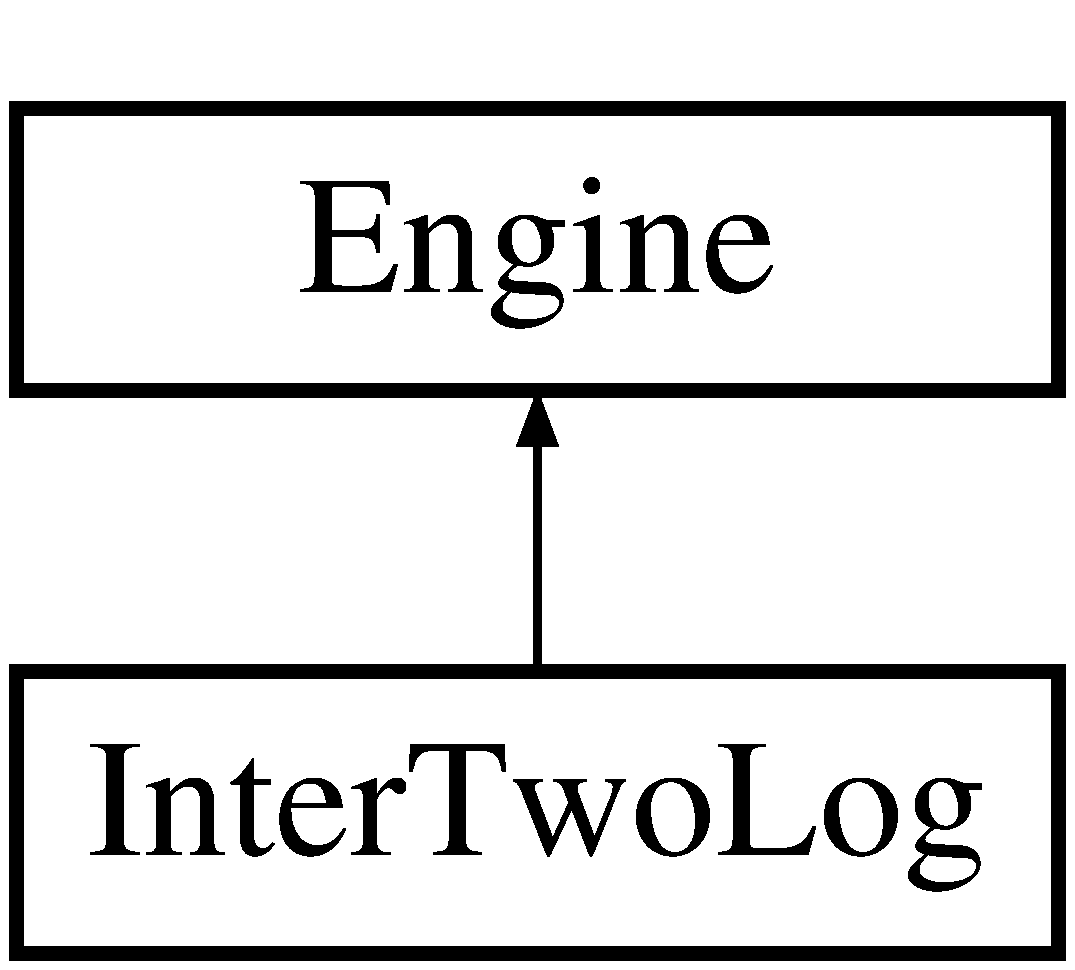
\includegraphics[height=2cm]{classInterTwoLog}
\end{center}
\end{figure}
\subsection*{Public Member Functions}
\begin{DoxyCompactItemize}
\item 
\hyperlink{classInterTwoLog_a4a7f06e802d741bac0b9934dd68b1fd3}{InterTwoLog} ()
\item 
\hyperlink{classInterTwoLog_a95e66b67f292f3bdd719fb6d57adcf1e}{$\sim$InterTwoLog} ()
\item 
virtual void \hyperlink{classInterTwoLog_af5dbc57497069c182c6101211fe2b64a}{init} ()
\item 
virtual void \hyperlink{classInterTwoLog_a581fcf71571bce5c0861e963c16f220b}{preProcess} ()
\item 
virtual void \hyperlink{classInterTwoLog_abd4e1bdf33314432d4a57193de056905}{process} ()
\item 
virtual void \hyperlink{classInterTwoLog_aa96d91206c19b781d222f0d6e13bf51d}{enslave} (\hyperlink{classEngineParamReader}{EngineParamReader} $\ast$)
\item 
virtual void \hyperlink{classInterTwoLog_a525b88900b11ed13cdefd73f5024e2eb}{test} ()
\end{DoxyCompactItemize}
\subsection*{Protected Member Functions}
\begin{DoxyCompactItemize}
\item 
void \hyperlink{classInterTwoLog_a01c7c507e0f2e66d38da544cd68cb76e}{delete\_\-my\_\-innards} ()
\item 
void \hyperlink{classInterTwoLog_ac83b4a0881e7d882fad88e25833cc565}{processPair} (int i, int j, \hyperlink{structInterTwoLogMeasures}{InterTwoLogMeasures} \&itlm)
\end{DoxyCompactItemize}
\subsection*{Protected Attributes}
\begin{DoxyCompactItemize}
\item 
\hyperlink{classEngineParamReader}{EngineParamReader} $\ast$ \hyperlink{classInterTwoLog_a1a1c375b7f30632abd59d0f2f61fc626}{itl\_\-param}
\item 
bool \hyperlink{classInterTwoLog_a5e71ddd55de30562ad4f92519bee43de}{haveOwner}
\item 
\hyperlink{classInterTwoLogOutput}{InterTwoLogOutput} \hyperlink{classInterTwoLog_a25742365edccdd4b3be23f85a39d942a}{out}
\item 
int \hyperlink{classInterTwoLog_abc10f45a18be673c9da60e34e34407a1}{numInitSNPs}
\item 
int \hyperlink{classInterTwoLog_aa36dd9a588d9b0ad8a322ac3672f22f0}{numInitPhen}
\item 
int \hyperlink{classInterTwoLog_a039b29fdef4854a0c85ae37bd2547a26}{numFinalPhen}
\item 
int \hyperlink{classInterTwoLog_ab677684383a49037019f4288a08983f3}{numCase}
\end{DoxyCompactItemize}


\subsection{Detailed Description}
\begin{DoxyAuthor}{Author}
Richard T. Guy
\end{DoxyAuthor}
Perform adjusted logistic regression search for interaction using the following model:

logit(y) = beta\_\-0 + beta $\ast$ covariates + beta\_\-\{n-\/2\} $\ast$ snp1 + beta\_\-\{n-\/1\} $\ast$ snp2 + beta\_\-n $\ast$ (snp1-\/mu1) $\ast$ (snp2-\/mu2)

Test H\_\-0: beta\_\-n = 0 using Wald test. 

\subsection{Constructor \& Destructor Documentation}
\hypertarget{classInterTwoLog_a4a7f06e802d741bac0b9934dd68b1fd3}{
\index{InterTwoLog@{InterTwoLog}!InterTwoLog@{InterTwoLog}}
\index{InterTwoLog@{InterTwoLog}!InterTwoLog@{InterTwoLog}}
\subsubsection[{InterTwoLog}]{\setlength{\rightskip}{0pt plus 5cm}InterTwoLog::InterTwoLog ()\hspace{0.3cm}{\ttfamily  \mbox{[}explicit\mbox{]}}}}
\label{classInterTwoLog_a4a7f06e802d741bac0b9934dd68b1fd3}
\hypertarget{classInterTwoLog_a95e66b67f292f3bdd719fb6d57adcf1e}{
\index{InterTwoLog@{InterTwoLog}!$\sim$InterTwoLog@{$\sim$InterTwoLog}}
\index{$\sim$InterTwoLog@{$\sim$InterTwoLog}!InterTwoLog@{InterTwoLog}}
\subsubsection[{$\sim$InterTwoLog}]{\setlength{\rightskip}{0pt plus 5cm}InterTwoLog::$\sim$InterTwoLog ()}}
\label{classInterTwoLog_a95e66b67f292f3bdd719fb6d57adcf1e}


\subsection{Member Function Documentation}
\hypertarget{classInterTwoLog_a01c7c507e0f2e66d38da544cd68cb76e}{
\index{InterTwoLog@{InterTwoLog}!delete\_\-my\_\-innards@{delete\_\-my\_\-innards}}
\index{delete\_\-my\_\-innards@{delete\_\-my\_\-innards}!InterTwoLog@{InterTwoLog}}
\subsubsection[{delete\_\-my\_\-innards}]{\setlength{\rightskip}{0pt plus 5cm}void InterTwoLog::delete\_\-my\_\-innards ()\hspace{0.3cm}{\ttfamily  \mbox{[}protected\mbox{]}}}}
\label{classInterTwoLog_a01c7c507e0f2e66d38da544cd68cb76e}
\hypertarget{classInterTwoLog_aa96d91206c19b781d222f0d6e13bf51d}{
\index{InterTwoLog@{InterTwoLog}!enslave@{enslave}}
\index{enslave@{enslave}!InterTwoLog@{InterTwoLog}}
\subsubsection[{enslave}]{\setlength{\rightskip}{0pt plus 5cm}void InterTwoLog::enslave ({\bf EngineParamReader} $\ast$)\hspace{0.3cm}{\ttfamily  \mbox{[}virtual\mbox{]}}}}
\label{classInterTwoLog_aa96d91206c19b781d222f0d6e13bf51d}


Implements \hyperlink{classEngine_a023e094182312b1732fe53754c2fe5cb}{Engine}.

\hypertarget{classInterTwoLog_af5dbc57497069c182c6101211fe2b64a}{
\index{InterTwoLog@{InterTwoLog}!init@{init}}
\index{init@{init}!InterTwoLog@{InterTwoLog}}
\subsubsection[{init}]{\setlength{\rightskip}{0pt plus 5cm}void InterTwoLog::init ()\hspace{0.3cm}{\ttfamily  \mbox{[}virtual\mbox{]}}}}
\label{classInterTwoLog_af5dbc57497069c182c6101211fe2b64a}


Implements \hyperlink{classEngine_aaa054d596fb8ced6e3eb4bee208f8c3d}{Engine}.

\hypertarget{classInterTwoLog_a581fcf71571bce5c0861e963c16f220b}{
\index{InterTwoLog@{InterTwoLog}!preProcess@{preProcess}}
\index{preProcess@{preProcess}!InterTwoLog@{InterTwoLog}}
\subsubsection[{preProcess}]{\setlength{\rightskip}{0pt plus 5cm}void InterTwoLog::preProcess ()\hspace{0.3cm}{\ttfamily  \mbox{[}virtual\mbox{]}}}}
\label{classInterTwoLog_a581fcf71571bce5c0861e963c16f220b}


Implements \hyperlink{classEngine_aec7076b8979a13c96eceb362437dc68c}{Engine}.

\hypertarget{classInterTwoLog_abd4e1bdf33314432d4a57193de056905}{
\index{InterTwoLog@{InterTwoLog}!process@{process}}
\index{process@{process}!InterTwoLog@{InterTwoLog}}
\subsubsection[{process}]{\setlength{\rightskip}{0pt plus 5cm}void InterTwoLog::process ()\hspace{0.3cm}{\ttfamily  \mbox{[}virtual\mbox{]}}}}
\label{classInterTwoLog_abd4e1bdf33314432d4a57193de056905}


Implements \hyperlink{classEngine_a005f8e277c3dea16ea05803fba223db7}{Engine}.

\hypertarget{classInterTwoLog_ac83b4a0881e7d882fad88e25833cc565}{
\index{InterTwoLog@{InterTwoLog}!processPair@{processPair}}
\index{processPair@{processPair}!InterTwoLog@{InterTwoLog}}
\subsubsection[{processPair}]{\setlength{\rightskip}{0pt plus 5cm}void InterTwoLog::processPair (int {\em i}, \/  int {\em j}, \/  {\bf InterTwoLogMeasures} \& {\em itlm})\hspace{0.3cm}{\ttfamily  \mbox{[}protected\mbox{]}}}}
\label{classInterTwoLog_ac83b4a0881e7d882fad88e25833cc565}
Create data and run test for a single pair of SNPs given by i and j.


\begin{DoxyParams}{Parameters}
\item[{\em i}]First SNP \item[{\em j}]Second SNP \end{DoxyParams}
\begin{DoxyReturn}{Returns}
itlm Structure filled with p, beta, se. 
\end{DoxyReturn}
\hypertarget{classInterTwoLog_a525b88900b11ed13cdefd73f5024e2eb}{
\index{InterTwoLog@{InterTwoLog}!test@{test}}
\index{test@{test}!InterTwoLog@{InterTwoLog}}
\subsubsection[{test}]{\setlength{\rightskip}{0pt plus 5cm}void InterTwoLog::test ()\hspace{0.3cm}{\ttfamily  \mbox{[}virtual\mbox{]}}}}
\label{classInterTwoLog_a525b88900b11ed13cdefd73f5024e2eb}


Implements \hyperlink{classEngine_a2927c4a4263809453063ad482c6434a4}{Engine}.



\subsection{Field Documentation}
\hypertarget{classInterTwoLog_a5e71ddd55de30562ad4f92519bee43de}{
\index{InterTwoLog@{InterTwoLog}!haveOwner@{haveOwner}}
\index{haveOwner@{haveOwner}!InterTwoLog@{InterTwoLog}}
\subsubsection[{haveOwner}]{\setlength{\rightskip}{0pt plus 5cm}bool {\bf InterTwoLog::haveOwner}\hspace{0.3cm}{\ttfamily  \mbox{[}protected\mbox{]}}}}
\label{classInterTwoLog_a5e71ddd55de30562ad4f92519bee43de}
\hypertarget{classInterTwoLog_a1a1c375b7f30632abd59d0f2f61fc626}{
\index{InterTwoLog@{InterTwoLog}!itl\_\-param@{itl\_\-param}}
\index{itl\_\-param@{itl\_\-param}!InterTwoLog@{InterTwoLog}}
\subsubsection[{itl\_\-param}]{\setlength{\rightskip}{0pt plus 5cm}{\bf EngineParamReader}$\ast$ {\bf InterTwoLog::itl\_\-param}\hspace{0.3cm}{\ttfamily  \mbox{[}protected\mbox{]}}}}
\label{classInterTwoLog_a1a1c375b7f30632abd59d0f2f61fc626}
\hypertarget{classInterTwoLog_ab677684383a49037019f4288a08983f3}{
\index{InterTwoLog@{InterTwoLog}!numCase@{numCase}}
\index{numCase@{numCase}!InterTwoLog@{InterTwoLog}}
\subsubsection[{numCase}]{\setlength{\rightskip}{0pt plus 5cm}int {\bf InterTwoLog::numCase}\hspace{0.3cm}{\ttfamily  \mbox{[}protected\mbox{]}}}}
\label{classInterTwoLog_ab677684383a49037019f4288a08983f3}
\hypertarget{classInterTwoLog_a039b29fdef4854a0c85ae37bd2547a26}{
\index{InterTwoLog@{InterTwoLog}!numFinalPhen@{numFinalPhen}}
\index{numFinalPhen@{numFinalPhen}!InterTwoLog@{InterTwoLog}}
\subsubsection[{numFinalPhen}]{\setlength{\rightskip}{0pt plus 5cm}int {\bf InterTwoLog::numFinalPhen}\hspace{0.3cm}{\ttfamily  \mbox{[}protected\mbox{]}}}}
\label{classInterTwoLog_a039b29fdef4854a0c85ae37bd2547a26}
\hypertarget{classInterTwoLog_aa36dd9a588d9b0ad8a322ac3672f22f0}{
\index{InterTwoLog@{InterTwoLog}!numInitPhen@{numInitPhen}}
\index{numInitPhen@{numInitPhen}!InterTwoLog@{InterTwoLog}}
\subsubsection[{numInitPhen}]{\setlength{\rightskip}{0pt plus 5cm}int {\bf InterTwoLog::numInitPhen}\hspace{0.3cm}{\ttfamily  \mbox{[}protected\mbox{]}}}}
\label{classInterTwoLog_aa36dd9a588d9b0ad8a322ac3672f22f0}
\hypertarget{classInterTwoLog_abc10f45a18be673c9da60e34e34407a1}{
\index{InterTwoLog@{InterTwoLog}!numInitSNPs@{numInitSNPs}}
\index{numInitSNPs@{numInitSNPs}!InterTwoLog@{InterTwoLog}}
\subsubsection[{numInitSNPs}]{\setlength{\rightskip}{0pt plus 5cm}int {\bf InterTwoLog::numInitSNPs}\hspace{0.3cm}{\ttfamily  \mbox{[}protected\mbox{]}}}}
\label{classInterTwoLog_abc10f45a18be673c9da60e34e34407a1}
\hypertarget{classInterTwoLog_a25742365edccdd4b3be23f85a39d942a}{
\index{InterTwoLog@{InterTwoLog}!out@{out}}
\index{out@{out}!InterTwoLog@{InterTwoLog}}
\subsubsection[{out}]{\setlength{\rightskip}{0pt plus 5cm}{\bf InterTwoLogOutput} {\bf InterTwoLog::out}\hspace{0.3cm}{\ttfamily  \mbox{[}protected\mbox{]}}}}
\label{classInterTwoLog_a25742365edccdd4b3be23f85a39d942a}


The documentation for this class was generated from the following files:\begin{DoxyCompactItemize}
\item 
engine/intertwolog/\hyperlink{intertwolog_8hh}{intertwolog.hh}\item 
engine/intertwolog/\hyperlink{intertwolog_8cpp}{intertwolog.cpp}\end{DoxyCompactItemize}

\hypertarget{structInterTwoLogMeasures}{
\section{InterTwoLogMeasures Struct Reference}
\label{structInterTwoLogMeasures}\index{InterTwoLogMeasures@{InterTwoLogMeasures}}
}


{\ttfamily \#include $<$intertwolog\_\-out.hh$>$}

\subsection*{Data Fields}
\begin{DoxyCompactItemize}
\item 
int \hyperlink{structInterTwoLogMeasures_a94b6a0b09c1c97b3d0125ddc76628448}{index1}
\item 
string \hyperlink{structInterTwoLogMeasures_a8de68e6596ff089ceb961142efd1511f}{name1}
\item 
string \hyperlink{structInterTwoLogMeasures_ae2674bca1f6256b7ffee69a6753223fa}{name2}
\item 
int \hyperlink{structInterTwoLogMeasures_af119c8d5a38d1c9be1e27298d34c3fe4}{index2}
\item 
double \hyperlink{structInterTwoLogMeasures_acc51a0307cefa7e90cac00b59e73c492}{pVal}
\item 
double \hyperlink{structInterTwoLogMeasures_ae0e2cfc789fa924b472556e5bb9e3412}{beta}
\item 
double \hyperlink{structInterTwoLogMeasures_a30ea64299ac79791bf47cda86b350fdd}{SE}
\end{DoxyCompactItemize}


\subsection{Field Documentation}
\hypertarget{structInterTwoLogMeasures_ae0e2cfc789fa924b472556e5bb9e3412}{
\index{InterTwoLogMeasures@{InterTwoLogMeasures}!beta@{beta}}
\index{beta@{beta}!InterTwoLogMeasures@{InterTwoLogMeasures}}
\subsubsection[{beta}]{\setlength{\rightskip}{0pt plus 5cm}double {\bf InterTwoLogMeasures::beta}}}
\label{structInterTwoLogMeasures_ae0e2cfc789fa924b472556e5bb9e3412}
\hypertarget{structInterTwoLogMeasures_a94b6a0b09c1c97b3d0125ddc76628448}{
\index{InterTwoLogMeasures@{InterTwoLogMeasures}!index1@{index1}}
\index{index1@{index1}!InterTwoLogMeasures@{InterTwoLogMeasures}}
\subsubsection[{index1}]{\setlength{\rightskip}{0pt plus 5cm}int {\bf InterTwoLogMeasures::index1}}}
\label{structInterTwoLogMeasures_a94b6a0b09c1c97b3d0125ddc76628448}
\hypertarget{structInterTwoLogMeasures_af119c8d5a38d1c9be1e27298d34c3fe4}{
\index{InterTwoLogMeasures@{InterTwoLogMeasures}!index2@{index2}}
\index{index2@{index2}!InterTwoLogMeasures@{InterTwoLogMeasures}}
\subsubsection[{index2}]{\setlength{\rightskip}{0pt plus 5cm}int {\bf InterTwoLogMeasures::index2}}}
\label{structInterTwoLogMeasures_af119c8d5a38d1c9be1e27298d34c3fe4}
\hypertarget{structInterTwoLogMeasures_a8de68e6596ff089ceb961142efd1511f}{
\index{InterTwoLogMeasures@{InterTwoLogMeasures}!name1@{name1}}
\index{name1@{name1}!InterTwoLogMeasures@{InterTwoLogMeasures}}
\subsubsection[{name1}]{\setlength{\rightskip}{0pt plus 5cm}string {\bf InterTwoLogMeasures::name1}}}
\label{structInterTwoLogMeasures_a8de68e6596ff089ceb961142efd1511f}
\hypertarget{structInterTwoLogMeasures_ae2674bca1f6256b7ffee69a6753223fa}{
\index{InterTwoLogMeasures@{InterTwoLogMeasures}!name2@{name2}}
\index{name2@{name2}!InterTwoLogMeasures@{InterTwoLogMeasures}}
\subsubsection[{name2}]{\setlength{\rightskip}{0pt plus 5cm}string {\bf InterTwoLogMeasures::name2}}}
\label{structInterTwoLogMeasures_ae2674bca1f6256b7ffee69a6753223fa}
\hypertarget{structInterTwoLogMeasures_acc51a0307cefa7e90cac00b59e73c492}{
\index{InterTwoLogMeasures@{InterTwoLogMeasures}!pVal@{pVal}}
\index{pVal@{pVal}!InterTwoLogMeasures@{InterTwoLogMeasures}}
\subsubsection[{pVal}]{\setlength{\rightskip}{0pt plus 5cm}double {\bf InterTwoLogMeasures::pVal}}}
\label{structInterTwoLogMeasures_acc51a0307cefa7e90cac00b59e73c492}
\hypertarget{structInterTwoLogMeasures_a30ea64299ac79791bf47cda86b350fdd}{
\index{InterTwoLogMeasures@{InterTwoLogMeasures}!SE@{SE}}
\index{SE@{SE}!InterTwoLogMeasures@{InterTwoLogMeasures}}
\subsubsection[{SE}]{\setlength{\rightskip}{0pt plus 5cm}double {\bf InterTwoLogMeasures::SE}}}
\label{structInterTwoLogMeasures_a30ea64299ac79791bf47cda86b350fdd}


The documentation for this struct was generated from the following file:\begin{DoxyCompactItemize}
\item 
engine/output/\hyperlink{intertwolog__out_8hh}{intertwolog\_\-out.hh}\end{DoxyCompactItemize}

\hypertarget{classInterTwoLogOutput}{
\section{InterTwoLogOutput Class Reference}
\label{classInterTwoLogOutput}\index{InterTwoLogOutput@{InterTwoLogOutput}}
}


{\ttfamily \#include $<$intertwolog\_\-out.hh$>$}

\subsection*{Public Member Functions}
\begin{DoxyCompactItemize}
\item 
\hyperlink{classInterTwoLogOutput_a22e75592762dfde6d82bc911aa810354}{InterTwoLogOutput} ()
\item 
\hyperlink{classInterTwoLogOutput_a6e6f407ccb2ae032b2758f9d1331a798}{$\sim$InterTwoLogOutput} ()
\item 
bool \hyperlink{classInterTwoLogOutput_a6bf1b2c7e2f158d2484cafaf08ff4a7c}{init} (\hyperlink{classParamReader}{ParamReader} $\ast$, \hyperlink{classEngineParamReader}{EngineParamReader} $\ast$, int maxMapSize, string message)
\item 
void \hyperlink{classInterTwoLogOutput_a81ed7b00f76b57d81bc4e504d9f36c66}{close} ()
\end{DoxyCompactItemize}
\subsection*{Protected Member Functions}
\begin{DoxyCompactItemize}
\item 
void \hyperlink{classInterTwoLogOutput_ae4cccc1f183d1d224e77360d00b9f3b9}{printLine} (const \hyperlink{structInterTwoLogMeasures}{InterTwoLogMeasures} \&itlo, int order)
\item 
void \hyperlink{classInterTwoLogOutput_ac8520bd89a481e5c17cffc75cde31671}{writeMainHeader} (\hyperlink{classParamReader}{ParamReader} $\ast$param)
\item 
void \hyperlink{classInterTwoLogOutput_a5cc1b8305c6233048ec3b4274a2323e2}{writeMainLegend} ()
\item 
void \hyperlink{classInterTwoLogOutput_a4856f3d92e9d3c691f991797825d1bcc}{writeLogHead} (\hyperlink{classParamReader}{ParamReader} $\ast$param)
\end{DoxyCompactItemize}
\subsection*{Protected Attributes}
\begin{DoxyCompactItemize}
\item 
\hyperlink{classOutput}{Output} \hyperlink{classInterTwoLogOutput_a66141117813508a67681b020e5113e7e}{out}
\item 
int \hyperlink{classInterTwoLogOutput_abb92f43d8630b9695545b28fdece04f5}{mapSize}
\end{DoxyCompactItemize}
\subsection*{Friends}
\begin{DoxyCompactItemize}
\item 
class \hyperlink{classInterTwoLogOutput_a3e7fc64b26065625ba57d692b5e411ca}{InterTwoLog}
\end{DoxyCompactItemize}


\subsection{Constructor \& Destructor Documentation}
\hypertarget{classInterTwoLogOutput_a22e75592762dfde6d82bc911aa810354}{
\index{InterTwoLogOutput@{InterTwoLogOutput}!InterTwoLogOutput@{InterTwoLogOutput}}
\index{InterTwoLogOutput@{InterTwoLogOutput}!InterTwoLogOutput@{InterTwoLogOutput}}
\subsubsection[{InterTwoLogOutput}]{\setlength{\rightskip}{0pt plus 5cm}InterTwoLogOutput::InterTwoLogOutput ()}}
\label{classInterTwoLogOutput_a22e75592762dfde6d82bc911aa810354}
\hypertarget{classInterTwoLogOutput_a6e6f407ccb2ae032b2758f9d1331a798}{
\index{InterTwoLogOutput@{InterTwoLogOutput}!$\sim$InterTwoLogOutput@{$\sim$InterTwoLogOutput}}
\index{$\sim$InterTwoLogOutput@{$\sim$InterTwoLogOutput}!InterTwoLogOutput@{InterTwoLogOutput}}
\subsubsection[{$\sim$InterTwoLogOutput}]{\setlength{\rightskip}{0pt plus 5cm}InterTwoLogOutput::$\sim$InterTwoLogOutput ()}}
\label{classInterTwoLogOutput_a6e6f407ccb2ae032b2758f9d1331a798}


\subsection{Member Function Documentation}
\hypertarget{classInterTwoLogOutput_a81ed7b00f76b57d81bc4e504d9f36c66}{
\index{InterTwoLogOutput@{InterTwoLogOutput}!close@{close}}
\index{close@{close}!InterTwoLogOutput@{InterTwoLogOutput}}
\subsubsection[{close}]{\setlength{\rightskip}{0pt plus 5cm}void InterTwoLogOutput::close ()}}
\label{classInterTwoLogOutput_a81ed7b00f76b57d81bc4e504d9f36c66}
\hypertarget{classInterTwoLogOutput_a6bf1b2c7e2f158d2484cafaf08ff4a7c}{
\index{InterTwoLogOutput@{InterTwoLogOutput}!init@{init}}
\index{init@{init}!InterTwoLogOutput@{InterTwoLogOutput}}
\subsubsection[{init}]{\setlength{\rightskip}{0pt plus 5cm}bool InterTwoLogOutput::init ({\bf ParamReader} $\ast$ {\em param}, \/  {\bf EngineParamReader} $\ast$ {\em eparams}, \/  int {\em maxMapSize}, \/  string {\em message})}}
\label{classInterTwoLogOutput_a6bf1b2c7e2f158d2484cafaf08ff4a7c}
\hypertarget{classInterTwoLogOutput_ae4cccc1f183d1d224e77360d00b9f3b9}{
\index{InterTwoLogOutput@{InterTwoLogOutput}!printLine@{printLine}}
\index{printLine@{printLine}!InterTwoLogOutput@{InterTwoLogOutput}}
\subsubsection[{printLine}]{\setlength{\rightskip}{0pt plus 5cm}void InterTwoLogOutput::printLine (const {\bf InterTwoLogMeasures} \& {\em itlo}, \/  int {\em order})\hspace{0.3cm}{\ttfamily  \mbox{[}protected\mbox{]}}}}
\label{classInterTwoLogOutput_ae4cccc1f183d1d224e77360d00b9f3b9}
\hypertarget{classInterTwoLogOutput_a4856f3d92e9d3c691f991797825d1bcc}{
\index{InterTwoLogOutput@{InterTwoLogOutput}!writeLogHead@{writeLogHead}}
\index{writeLogHead@{writeLogHead}!InterTwoLogOutput@{InterTwoLogOutput}}
\subsubsection[{writeLogHead}]{\setlength{\rightskip}{0pt plus 5cm}void InterTwoLogOutput::writeLogHead ({\bf ParamReader} $\ast$ {\em param})\hspace{0.3cm}{\ttfamily  \mbox{[}protected\mbox{]}}}}
\label{classInterTwoLogOutput_a4856f3d92e9d3c691f991797825d1bcc}
Write a header to the logging file. \hypertarget{classInterTwoLogOutput_ac8520bd89a481e5c17cffc75cde31671}{
\index{InterTwoLogOutput@{InterTwoLogOutput}!writeMainHeader@{writeMainHeader}}
\index{writeMainHeader@{writeMainHeader}!InterTwoLogOutput@{InterTwoLogOutput}}
\subsubsection[{writeMainHeader}]{\setlength{\rightskip}{0pt plus 5cm}void InterTwoLogOutput::writeMainHeader ({\bf ParamReader} $\ast$ {\em param})\hspace{0.3cm}{\ttfamily  \mbox{[}protected\mbox{]}}}}
\label{classInterTwoLogOutput_ac8520bd89a481e5c17cffc75cde31671}
\hypertarget{classInterTwoLogOutput_a5cc1b8305c6233048ec3b4274a2323e2}{
\index{InterTwoLogOutput@{InterTwoLogOutput}!writeMainLegend@{writeMainLegend}}
\index{writeMainLegend@{writeMainLegend}!InterTwoLogOutput@{InterTwoLogOutput}}
\subsubsection[{writeMainLegend}]{\setlength{\rightskip}{0pt plus 5cm}void InterTwoLogOutput::writeMainLegend ()\hspace{0.3cm}{\ttfamily  \mbox{[}protected\mbox{]}}}}
\label{classInterTwoLogOutput_a5cc1b8305c6233048ec3b4274a2323e2}


\subsection{Friends And Related Function Documentation}
\hypertarget{classInterTwoLogOutput_a3e7fc64b26065625ba57d692b5e411ca}{
\index{InterTwoLogOutput@{InterTwoLogOutput}!InterTwoLog@{InterTwoLog}}
\index{InterTwoLog@{InterTwoLog}!InterTwoLogOutput@{InterTwoLogOutput}}
\subsubsection[{InterTwoLog}]{\setlength{\rightskip}{0pt plus 5cm}friend class {\bf InterTwoLog}\hspace{0.3cm}{\ttfamily  \mbox{[}friend\mbox{]}}}}
\label{classInterTwoLogOutput_a3e7fc64b26065625ba57d692b5e411ca}


\subsection{Field Documentation}
\hypertarget{classInterTwoLogOutput_abb92f43d8630b9695545b28fdece04f5}{
\index{InterTwoLogOutput@{InterTwoLogOutput}!mapSize@{mapSize}}
\index{mapSize@{mapSize}!InterTwoLogOutput@{InterTwoLogOutput}}
\subsubsection[{mapSize}]{\setlength{\rightskip}{0pt plus 5cm}int {\bf InterTwoLogOutput::mapSize}\hspace{0.3cm}{\ttfamily  \mbox{[}protected\mbox{]}}}}
\label{classInterTwoLogOutput_abb92f43d8630b9695545b28fdece04f5}
\hypertarget{classInterTwoLogOutput_a66141117813508a67681b020e5113e7e}{
\index{InterTwoLogOutput@{InterTwoLogOutput}!out@{out}}
\index{out@{out}!InterTwoLogOutput@{InterTwoLogOutput}}
\subsubsection[{out}]{\setlength{\rightskip}{0pt plus 5cm}{\bf Output} {\bf InterTwoLogOutput::out}\hspace{0.3cm}{\ttfamily  \mbox{[}protected\mbox{]}}}}
\label{classInterTwoLogOutput_a66141117813508a67681b020e5113e7e}


The documentation for this class was generated from the following files:\begin{DoxyCompactItemize}
\item 
engine/output/\hyperlink{intertwolog__out_8hh}{intertwolog\_\-out.hh}\item 
engine/output/\hyperlink{intertwolog__out_8cpp}{intertwolog\_\-out.cpp}\end{DoxyCompactItemize}

\hypertarget{classInvalidChiSquareException}{
\section{InvalidChiSquareException Class Reference}
\label{classInvalidChiSquareException}\index{InvalidChiSquareException@{InvalidChiSquareException}}
}


{\ttfamily \#include $<$exceptions.h$>$}

Inheritance diagram for InvalidChiSquareException:\begin{figure}[H]
\begin{center}
\leavevmode
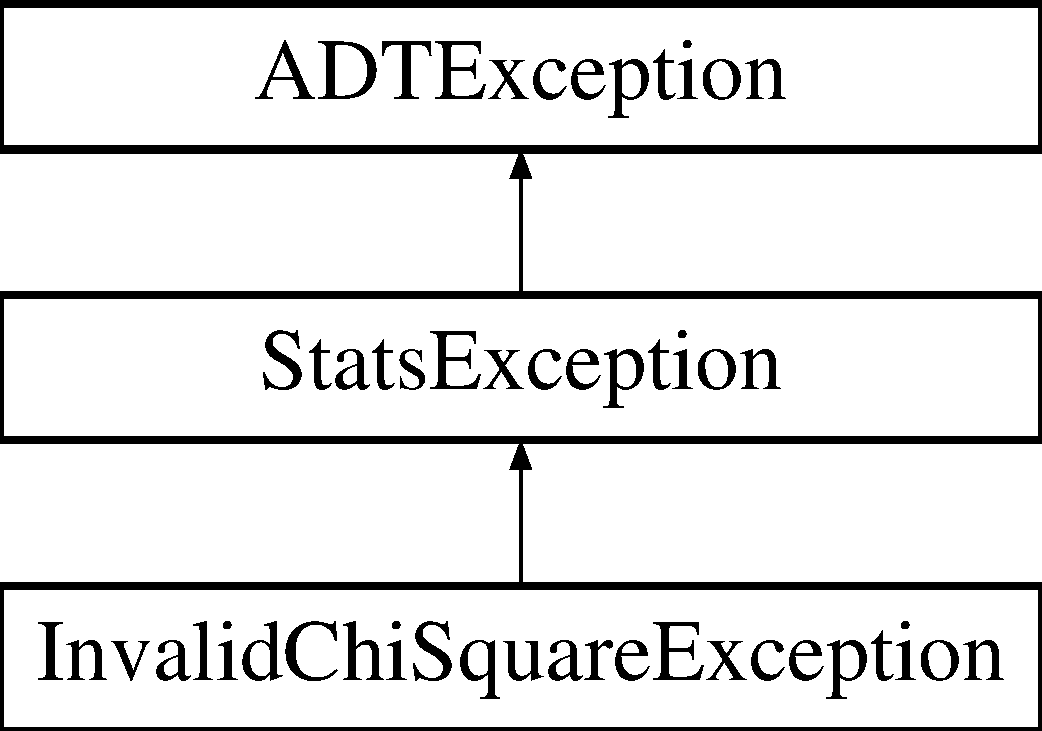
\includegraphics[height=3cm]{classInvalidChiSquareException}
\end{center}
\end{figure}


The documentation for this class was generated from the following file:\begin{DoxyCompactItemize}
\item 
engine/utils/\hyperlink{exceptions_8h}{exceptions.h}\end{DoxyCompactItemize}

\hypertarget{classInvalidNewRaphInputEx}{
\section{InvalidNewRaphInputEx Class Reference}
\label{classInvalidNewRaphInputEx}\index{InvalidNewRaphInputEx@{InvalidNewRaphInputEx}}
}


{\ttfamily \#include $<$exceptions.h$>$}

Inheritance diagram for InvalidNewRaphInputEx:\begin{figure}[H]
\begin{center}
\leavevmode
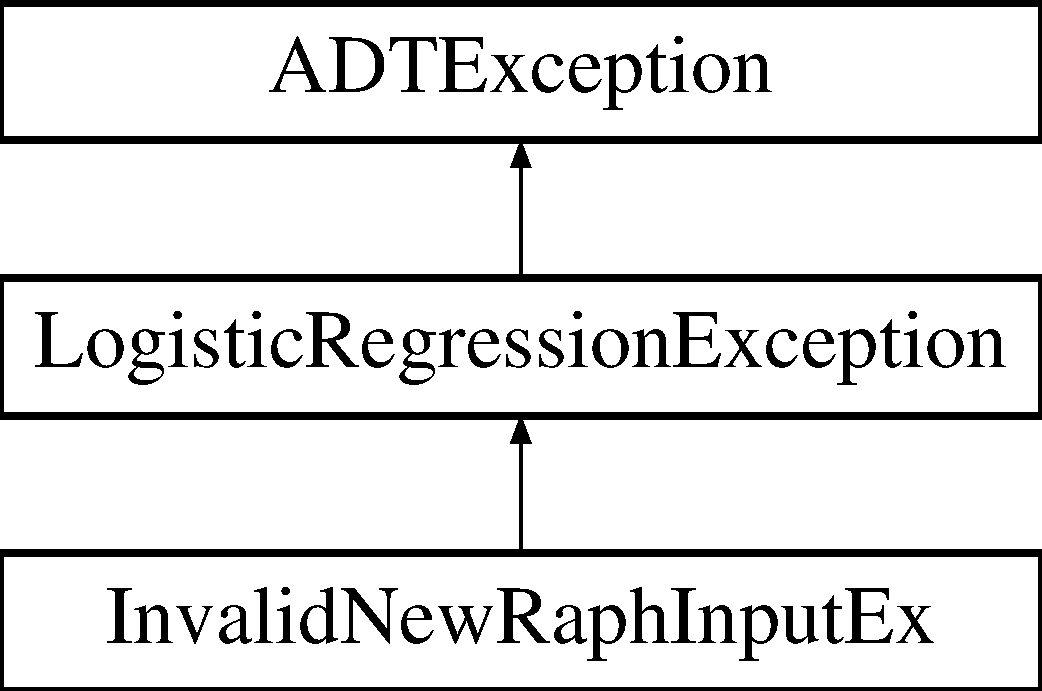
\includegraphics[height=3cm]{classInvalidNewRaphInputEx}
\end{center}
\end{figure}


The documentation for this class was generated from the following file:\begin{DoxyCompactItemize}
\item 
engine/utils/\hyperlink{exceptions_8h}{exceptions.h}\end{DoxyCompactItemize}

\hypertarget{classLinearRegression}{
\section{LinearRegression Class Reference}
\label{classLinearRegression}\index{LinearRegression@{LinearRegression}}
}


{\ttfamily \#include $<$linear\_\-regression.hh$>$}

\subsection*{Public Member Functions}
\begin{DoxyCompactItemize}
\item 
\hyperlink{classLinearRegression_afeb4c101e4e8b20a75db3d4ce3f1cbc6}{LinearRegression} ()
\item 
vector$<$ double $>$ \hyperlink{classLinearRegression_a37f79d0d49e5fe93cf5a04b20d17d829}{leastSquares} (const vector$<$ vector$<$ double $>$ $>$ \&data, const vector$<$ double $>$ \&response)
\item 
void \hyperlink{classLinearRegression_a54ba438eebfb5045c7e6d02545adf346}{sumSquaredStats} (const vector$<$ vector$<$ double $>$ $>$ \&data, const vector$<$ double $>$ \&betas, const vector$<$ double $>$ \&response, double mean, double \&sse, double \&ssr)
\item 
vector$<$ double $>$ \hyperlink{classLinearRegression_a1c6ed479606439a1943f75c888e8f2bd}{residuals} (const vector$<$ vector$<$ double $>$ $>$ \&data, const vector$<$ double $>$ \&betas, const vector$<$ double $>$ \&response)
\item 
double \hyperlink{classLinearRegression_affb7f28584f32975adf12f3a624cfe15}{anova} (const vector$<$ double $>$ \&response, const vector$<$ double $>$ \&division, double means\mbox{[}4\mbox{]})
\item 
void \hyperlink{classLinearRegression_a866934791e5415bf573a9030650ef8cb}{test} ()
\end{DoxyCompactItemize}


\subsection{Constructor \& Destructor Documentation}
\hypertarget{classLinearRegression_afeb4c101e4e8b20a75db3d4ce3f1cbc6}{
\index{LinearRegression@{LinearRegression}!LinearRegression@{LinearRegression}}
\index{LinearRegression@{LinearRegression}!LinearRegression@{LinearRegression}}
\subsubsection[{LinearRegression}]{\setlength{\rightskip}{0pt plus 5cm}LinearRegression::LinearRegression ()}}
\label{classLinearRegression_afeb4c101e4e8b20a75db3d4ce3f1cbc6}


\subsection{Member Function Documentation}
\hypertarget{classLinearRegression_affb7f28584f32975adf12f3a624cfe15}{
\index{LinearRegression@{LinearRegression}!anova@{anova}}
\index{anova@{anova}!LinearRegression@{LinearRegression}}
\subsubsection[{anova}]{\setlength{\rightskip}{0pt plus 5cm}double LinearRegression::anova (const vector$<$ double $>$ \& {\em response}, \/  const vector$<$ double $>$ \& {\em division}, \/  double {\em means}\mbox{[}4\mbox{]})}}
\label{classLinearRegression_affb7f28584f32975adf12f3a624cfe15}
Anova of the response variable. In practice, this is called from the genostats::compLinRegStats method using the calculated genotype from the additive model. That is why we expect -\/1,0,1 coding.


\begin{DoxyParams}{Parameters}
\item[{\em response}]Vector of response variables. \item[{\em division}]Vector of SNP variables. Expects -\/1,0,1 coding. \item[{\em means\mbox{[}3\mbox{]}}]holds mean(-\/1), mean(0), mean(1), mean(tot) where mean is of response variable. \end{DoxyParams}
\hypertarget{classLinearRegression_a37f79d0d49e5fe93cf5a04b20d17d829}{
\index{LinearRegression@{LinearRegression}!leastSquares@{leastSquares}}
\index{leastSquares@{leastSquares}!LinearRegression@{LinearRegression}}
\subsubsection[{leastSquares}]{\setlength{\rightskip}{0pt plus 5cm}vector$<$ double $>$ LinearRegression::leastSquares (const vector$<$ vector$<$ double $>$ $>$ \& {\em data}, \/  const vector$<$ double $>$ \& {\em response})}}
\label{classLinearRegression_a37f79d0d49e5fe93cf5a04b20d17d829}
Compute the ordinary least squares estimation of the solution to a linear regression


\begin{DoxyParams}{Parameters}
\item[{\em data}]The regression input. Each inner vector should be a single variable (so column maj order) \item[{\em response}]The response variable. \end{DoxyParams}
\begin{DoxyReturn}{Returns}
betas The estimate of regression coefficients 
\end{DoxyReturn}


X'$\ast$X

X'$\ast$beta

tempSquare $\ast$ tempWork 

\hypertarget{classLinearRegression_a1c6ed479606439a1943f75c888e8f2bd}{
\index{LinearRegression@{LinearRegression}!residuals@{residuals}}
\index{residuals@{residuals}!LinearRegression@{LinearRegression}}
\subsubsection[{residuals}]{\setlength{\rightskip}{0pt plus 5cm}vector$<$ double $>$ LinearRegression::residuals (const vector$<$ vector$<$ double $>$ $>$ \& {\em data}, \/  const vector$<$ double $>$ \& {\em betas}, \/  const vector$<$ double $>$ \& {\em response})}}
\label{classLinearRegression_a1c6ed479606439a1943f75c888e8f2bd}
Compute the residuals of a given parameter set betas.


\begin{DoxyParams}{Parameters}
\item[{\em data}]vector of vectors. \item[{\em betas}]vector of parameters \item[{\em response}]vector of dependent variable values. \end{DoxyParams}
\hypertarget{classLinearRegression_a54ba438eebfb5045c7e6d02545adf346}{
\index{LinearRegression@{LinearRegression}!sumSquaredStats@{sumSquaredStats}}
\index{sumSquaredStats@{sumSquaredStats}!LinearRegression@{LinearRegression}}
\subsubsection[{sumSquaredStats}]{\setlength{\rightskip}{0pt plus 5cm}void LinearRegression::sumSquaredStats (const vector$<$ vector$<$ double $>$ $>$ \& {\em data}, \/  const vector$<$ double $>$ \& {\em betas}, \/  const vector$<$ double $>$ \& {\em response}, \/  double {\em mean}, \/  double \& {\em sse}, \/  double \& {\em ssr})}}
\label{classLinearRegression_a54ba438eebfb5045c7e6d02545adf346}
Compute the sum of squared errors for a given set of beta coefficients.


\begin{DoxyParams}{Parameters}
\item[{\em data}]The regression input. Each inner vector is a single variable. \item[{\em betas}]The betas to be compared. \item[{\em response}]The response to compare against. \item[{\em mean}]The mean of the response variable \end{DoxyParams}
\begin{DoxyReturn}{Returns}
sse The sum squared error 

ssr The sum squared residual. 
\end{DoxyReturn}
\hypertarget{classLinearRegression_a866934791e5415bf573a9030650ef8cb}{
\index{LinearRegression@{LinearRegression}!test@{test}}
\index{test@{test}!LinearRegression@{LinearRegression}}
\subsubsection[{test}]{\setlength{\rightskip}{0pt plus 5cm}void LinearRegression::test ()}}
\label{classLinearRegression_a866934791e5415bf573a9030650ef8cb}


The documentation for this class was generated from the following files:\begin{DoxyCompactItemize}
\item 
engine/utils/\hyperlink{linear__regression_8hh}{linear\_\-regression.hh}\item 
engine/utils/\hyperlink{linear__regression_8cpp}{linear\_\-regression.cpp}\end{DoxyCompactItemize}

\hypertarget{classLinearRegressionException}{
\section{LinearRegressionException Class Reference}
\label{classLinearRegressionException}\index{LinearRegressionException@{LinearRegressionException}}
}


{\ttfamily \#include $<$exceptions.h$>$}

Inheritance diagram for LinearRegressionException:\begin{figure}[H]
\begin{center}
\leavevmode
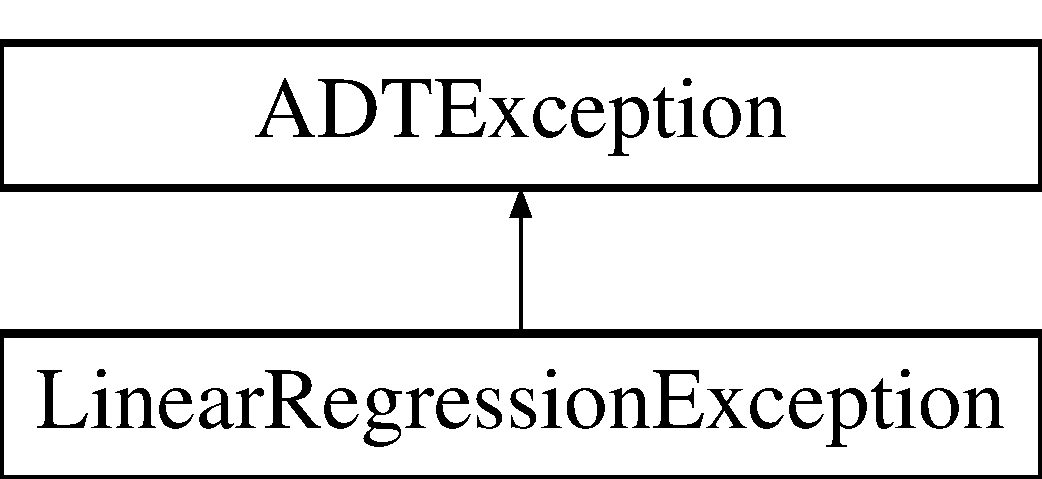
\includegraphics[height=2cm]{classLinearRegressionException}
\end{center}
\end{figure}


The documentation for this class was generated from the following file:\begin{DoxyCompactItemize}
\item 
engine/utils/\hyperlink{exceptions_8h}{exceptions.h}\end{DoxyCompactItemize}

\hypertarget{classLinkageDisequilibrium}{
\section{LinkageDisequilibrium Class Reference}
\label{classLinkageDisequilibrium}\index{LinkageDisequilibrium@{LinkageDisequilibrium}}
}


{\ttfamily \#include $<$ld.h$>$}

Inheritance diagram for LinkageDisequilibrium:\begin{figure}[H]
\begin{center}
\leavevmode
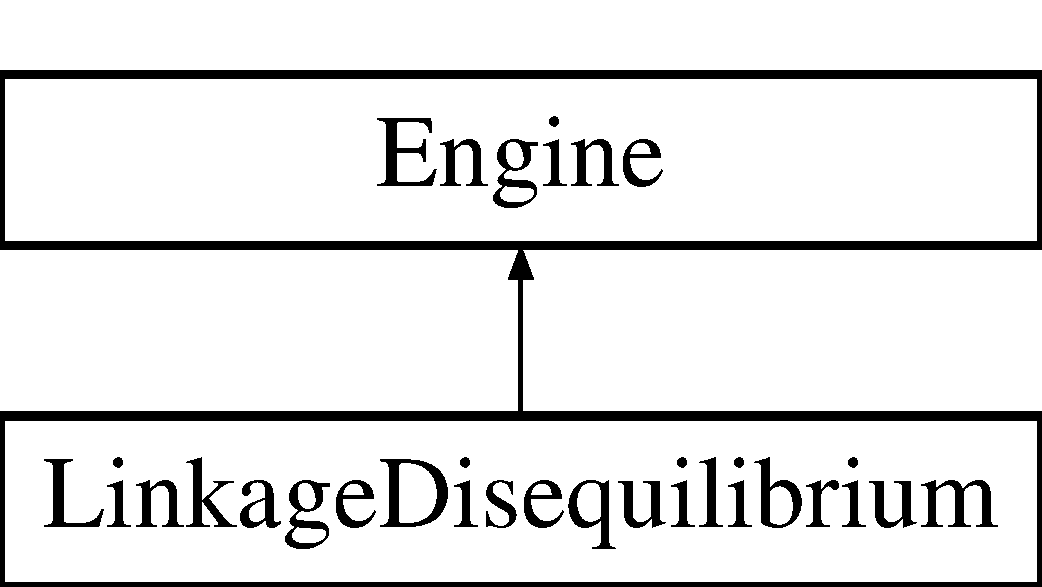
\includegraphics[height=2cm]{classLinkageDisequilibrium}
\end{center}
\end{figure}
\subsection*{Public Member Functions}
\begin{DoxyCompactItemize}
\item 
\hyperlink{classLinkageDisequilibrium_a2c865ee249f25e08594f44ca2fddedcc}{LinkageDisequilibrium} ()
\item 
\hyperlink{classLinkageDisequilibrium_a3cbd5550ac91f329d76fc7652a58edd5}{LinkageDisequilibrium} (\hyperlink{classDataAccess}{DataAccess} $\ast$)
\item 
\hyperlink{classLinkageDisequilibrium_a8c0492fd94c5c4b966ba10cad283baf1}{$\sim$LinkageDisequilibrium} ()
\item 
virtual void \hyperlink{classLinkageDisequilibrium_a9d3c50f9b7c3f5739ce12eb0b2068c6c}{init} ()
\item 
virtual void \hyperlink{classLinkageDisequilibrium_a2f466153298f2c868a78b5573f6c5048}{preProcess} ()
\item 
virtual void \hyperlink{classLinkageDisequilibrium_a821abc8314c8e6bddc1dfcdf24bdda09}{process} ()
\item 
virtual void \hyperlink{classLinkageDisequilibrium_afb777d3a63bbb0f2d23ce052de891023}{enslave} (\hyperlink{classEngineParamReader}{EngineParamReader} $\ast$)
\item 
virtual void \hyperlink{classLinkageDisequilibrium_a8df37823ab11776642f571e8e8ba7e3b}{test} ()
\item 
bool \hyperlink{classLinkageDisequilibrium_a11db054a2925bd82379a6b39a9f3464f}{dprimeOnPair} (int s1, int s2, \hyperlink{structLinkageMeasures}{LinkageMeasures} \&results)
\end{DoxyCompactItemize}
\subsection*{Static Public Member Functions}
\begin{DoxyCompactItemize}
\item 
static double \hyperlink{classLinkageDisequilibrium_a6207b7cc0fa21495363246ec41ee3164}{computeDPrime} (\hyperlink{classEM}{EM} \&, double aFreq\mbox{[}2\mbox{]}\mbox{[}3\mbox{]})
\item 
static double \hyperlink{classLinkageDisequilibrium_a24f37b16583031e1b335109fe0755a24}{dPrime} (int iallele, int jallele, double aFreq\mbox{[}2\mbox{]}\mbox{[}3\mbox{]}, const vector$<$ int $>$ \&, const vector$<$ double $>$ \&)
\item 
static double \hyperlink{classLinkageDisequilibrium_a368b63fa8f9f18804ad9f588c6bb4dbb}{compDee} (\hyperlink{classEM}{EM} \&e)
\item 
static double \hyperlink{classLinkageDisequilibrium_a94dde069bebfff0977e49d556c29fad4}{compRSquare} (double dee, double aFreq\mbox{[}2\mbox{]}\mbox{[}3\mbox{]})
\item 
static double \hyperlink{classLinkageDisequilibrium_a6a3f41206e3713204eaab35faf89c65b}{compDelta} (double dee, \hyperlink{classEM}{EM} \&e)
\end{DoxyCompactItemize}
\subsection*{Protected Member Functions}
\begin{DoxyCompactItemize}
\item 
void \hyperlink{classLinkageDisequilibrium_aae443ca228a7ae15b3611c1c6d8429ad}{delete\_\-my\_\-innards} ()
\end{DoxyCompactItemize}
\subsection*{Static Protected Member Functions}
\begin{DoxyCompactItemize}
\item 
static double \hyperlink{classLinkageDisequilibrium_a9920e98718ecb60c5b33c90ae2fb6c89}{EPS} ()
\end{DoxyCompactItemize}
\subsection*{Protected Attributes}
\begin{DoxyCompactItemize}
\item 
bool \hyperlink{classLinkageDisequilibrium_a1de71d86c97f892f29d165e2d37181b2}{haveOwner}
\item 
int \hyperlink{classLinkageDisequilibrium_a6bb08acf924aa961700b802095ff697e}{order\_\-in\_\-bag}
\item 
int \hyperlink{classLinkageDisequilibrium_af2487209d065ab6f7286beb76bc6b239}{window}
\item 
\hyperlink{classEngineParamReader}{EngineParamReader} $\ast$ \hyperlink{classLinkageDisequilibrium_a8b4887ba11facc45a5a4a84dea191db9}{ld\_\-param}
\item 
bool \hyperlink{classLinkageDisequilibrium_a635279ff05e69333abc2391b3a085d0c}{diagonal}
\item 
\hyperlink{classLinkageOutput}{LinkageOutput} \hyperlink{classLinkageDisequilibrium_ac3844fe848ba87fe5d26e12d7c6f20d8}{output}
\item 
int \hyperlink{classLinkageDisequilibrium_ab1132cf2922b184a6ba21c5c4b6c8a43}{numInitSNPs}
\item 
int \hyperlink{classLinkageDisequilibrium_afb85fd66b53951f9ea57ef0835a93260}{numInitPhen}
\item 
int \hyperlink{classLinkageDisequilibrium_a5f5bf8027d2e4a7cbac182d39014f93f}{numFinalPhen}
\end{DoxyCompactItemize}


\subsection{Detailed Description}
Linkage Disequilibrium computation class. Will perform diagonal or full model by calling \hyperlink{classLinkageDisequilibrium_a821abc8314c8e6bddc1dfcdf24bdda09}{process()}. Will perform LD between specified pair of SNPs as well.

\begin{DoxyAuthor}{Author}
Richard T. Guy (in present form) 

Joshua Grab, Matt Steigert, Carl D. Langefeld 
\end{DoxyAuthor}


\subsection{Constructor \& Destructor Documentation}
\hypertarget{classLinkageDisequilibrium_a2c865ee249f25e08594f44ca2fddedcc}{
\index{LinkageDisequilibrium@{LinkageDisequilibrium}!LinkageDisequilibrium@{LinkageDisequilibrium}}
\index{LinkageDisequilibrium@{LinkageDisequilibrium}!LinkageDisequilibrium@{LinkageDisequilibrium}}
\subsubsection[{LinkageDisequilibrium}]{\setlength{\rightskip}{0pt plus 5cm}LinkageDisequilibrium::LinkageDisequilibrium ()\hspace{0.3cm}{\ttfamily  \mbox{[}explicit\mbox{]}}}}
\label{classLinkageDisequilibrium_a2c865ee249f25e08594f44ca2fddedcc}
\hypertarget{classLinkageDisequilibrium_a3cbd5550ac91f329d76fc7652a58edd5}{
\index{LinkageDisequilibrium@{LinkageDisequilibrium}!LinkageDisequilibrium@{LinkageDisequilibrium}}
\index{LinkageDisequilibrium@{LinkageDisequilibrium}!LinkageDisequilibrium@{LinkageDisequilibrium}}
\subsubsection[{LinkageDisequilibrium}]{\setlength{\rightskip}{0pt plus 5cm}LinkageDisequilibrium::LinkageDisequilibrium ({\bf DataAccess} $\ast$ {\em data})\hspace{0.3cm}{\ttfamily  \mbox{[}explicit\mbox{]}}}}
\label{classLinkageDisequilibrium_a3cbd5550ac91f329d76fc7652a58edd5}
\hypertarget{classLinkageDisequilibrium_a8c0492fd94c5c4b966ba10cad283baf1}{
\index{LinkageDisequilibrium@{LinkageDisequilibrium}!$\sim$LinkageDisequilibrium@{$\sim$LinkageDisequilibrium}}
\index{$\sim$LinkageDisequilibrium@{$\sim$LinkageDisequilibrium}!LinkageDisequilibrium@{LinkageDisequilibrium}}
\subsubsection[{$\sim$LinkageDisequilibrium}]{\setlength{\rightskip}{0pt plus 5cm}LinkageDisequilibrium::$\sim$LinkageDisequilibrium ()}}
\label{classLinkageDisequilibrium_a8c0492fd94c5c4b966ba10cad283baf1}


\subsection{Member Function Documentation}
\hypertarget{classLinkageDisequilibrium_a368b63fa8f9f18804ad9f588c6bb4dbb}{
\index{LinkageDisequilibrium@{LinkageDisequilibrium}!compDee@{compDee}}
\index{compDee@{compDee}!LinkageDisequilibrium@{LinkageDisequilibrium}}
\subsubsection[{compDee}]{\setlength{\rightskip}{0pt plus 5cm}double LinkageDisequilibrium::compDee ({\bf EM} \& {\em e})\hspace{0.3cm}{\ttfamily  \mbox{[}static\mbox{]}}}}
\label{classLinkageDisequilibrium_a368b63fa8f9f18804ad9f588c6bb4dbb}
Compute D \hypertarget{classLinkageDisequilibrium_a6a3f41206e3713204eaab35faf89c65b}{
\index{LinkageDisequilibrium@{LinkageDisequilibrium}!compDelta@{compDelta}}
\index{compDelta@{compDelta}!LinkageDisequilibrium@{LinkageDisequilibrium}}
\subsubsection[{compDelta}]{\setlength{\rightskip}{0pt plus 5cm}double LinkageDisequilibrium::compDelta (double {\em dee}, \/  {\bf EM} \& {\em e})\hspace{0.3cm}{\ttfamily  \mbox{[}static\mbox{]}}}}
\label{classLinkageDisequilibrium_a6a3f41206e3713204eaab35faf89c65b}
\hypertarget{classLinkageDisequilibrium_a94dde069bebfff0977e49d556c29fad4}{
\index{LinkageDisequilibrium@{LinkageDisequilibrium}!compRSquare@{compRSquare}}
\index{compRSquare@{compRSquare}!LinkageDisequilibrium@{LinkageDisequilibrium}}
\subsubsection[{compRSquare}]{\setlength{\rightskip}{0pt plus 5cm}double LinkageDisequilibrium::compRSquare (double {\em dee}, \/  double {\em aFreq}\mbox{[}2\mbox{]}\mbox{[}3\mbox{]})\hspace{0.3cm}{\ttfamily  \mbox{[}static\mbox{]}}}}
\label{classLinkageDisequilibrium_a94dde069bebfff0977e49d556c29fad4}
\hypertarget{classLinkageDisequilibrium_a6207b7cc0fa21495363246ec41ee3164}{
\index{LinkageDisequilibrium@{LinkageDisequilibrium}!computeDPrime@{computeDPrime}}
\index{computeDPrime@{computeDPrime}!LinkageDisequilibrium@{LinkageDisequilibrium}}
\subsubsection[{computeDPrime}]{\setlength{\rightskip}{0pt plus 5cm}double LinkageDisequilibrium::computeDPrime ({\bf EM} \& {\em emAlg}, \/  double {\em aFreq}\mbox{[}2\mbox{]}\mbox{[}3\mbox{]})\hspace{0.3cm}{\ttfamily  \mbox{[}static\mbox{]}}}}
\label{classLinkageDisequilibrium_a6207b7cc0fa21495363246ec41ee3164}
Compute DPrime, from which all other measures are computed.


\begin{DoxyParams}{Parameters}
\item[{\em aFreq}]contains allele freqs in form A,a,B,b \item[{\em emAlg}]Contains an \hyperlink{classEM}{EM} object that includes data from previous run. \end{DoxyParams}
\begin{DoxyReturn}{Returns}
Dprime measurement. 
\end{DoxyReturn}
\hypertarget{classLinkageDisequilibrium_aae443ca228a7ae15b3611c1c6d8429ad}{
\index{LinkageDisequilibrium@{LinkageDisequilibrium}!delete\_\-my\_\-innards@{delete\_\-my\_\-innards}}
\index{delete\_\-my\_\-innards@{delete\_\-my\_\-innards}!LinkageDisequilibrium@{LinkageDisequilibrium}}
\subsubsection[{delete\_\-my\_\-innards}]{\setlength{\rightskip}{0pt plus 5cm}void LinkageDisequilibrium::delete\_\-my\_\-innards ()\hspace{0.3cm}{\ttfamily  \mbox{[}protected\mbox{]}}}}
\label{classLinkageDisequilibrium_aae443ca228a7ae15b3611c1c6d8429ad}
\hypertarget{classLinkageDisequilibrium_a24f37b16583031e1b335109fe0755a24}{
\index{LinkageDisequilibrium@{LinkageDisequilibrium}!dPrime@{dPrime}}
\index{dPrime@{dPrime}!LinkageDisequilibrium@{LinkageDisequilibrium}}
\subsubsection[{dPrime}]{\setlength{\rightskip}{0pt plus 5cm}double LinkageDisequilibrium::dPrime (int {\em iallele}, \/  int {\em jallele}, \/  double {\em aFreq}\mbox{[}2\mbox{]}\mbox{[}3\mbox{]}, \/  const vector$<$ int $>$ \& {\em numAlleles}, \/  const vector$<$ double $>$ \& {\em hapProbs})\hspace{0.3cm}{\ttfamily  \mbox{[}static\mbox{]}}}}
\label{classLinkageDisequilibrium_a24f37b16583031e1b335109fe0755a24}
Called by computeDPrime. \hypertarget{classLinkageDisequilibrium_a11db054a2925bd82379a6b39a9f3464f}{
\index{LinkageDisequilibrium@{LinkageDisequilibrium}!dprimeOnPair@{dprimeOnPair}}
\index{dprimeOnPair@{dprimeOnPair}!LinkageDisequilibrium@{LinkageDisequilibrium}}
\subsubsection[{dprimeOnPair}]{\setlength{\rightskip}{0pt plus 5cm}bool LinkageDisequilibrium::dprimeOnPair (int {\em s1}, \/  int {\em s2}, \/  {\bf LinkageMeasures} \& {\em lr})}}
\label{classLinkageDisequilibrium_a11db054a2925bd82379a6b39a9f3464f}
Perform all linkage disequilibrium measures on two SNPs


\begin{DoxyParams}{Parameters}
\item[{\em s1}]SNP 1 \item[{\em s2}]SNP 2 \end{DoxyParams}
\begin{DoxyReturn}{Returns}
lr A filled linkage measures struct.
\end{DoxyReturn}
\begin{Desc}
\item[\hyperlink{bug__bug000001}{Bug}]The error spits to cerr not logger. \end{Desc}
\hypertarget{classLinkageDisequilibrium_afb777d3a63bbb0f2d23ce052de891023}{
\index{LinkageDisequilibrium@{LinkageDisequilibrium}!enslave@{enslave}}
\index{enslave@{enslave}!LinkageDisequilibrium@{LinkageDisequilibrium}}
\subsubsection[{enslave}]{\setlength{\rightskip}{0pt plus 5cm}void LinkageDisequilibrium::enslave ({\bf EngineParamReader} $\ast$ {\em e})\hspace{0.3cm}{\ttfamily  \mbox{[}virtual\mbox{]}}}}
\label{classLinkageDisequilibrium_afb777d3a63bbb0f2d23ce052de891023}
Enslave this LD engine. For an LD engine, enslavement means that the output file name has to change and the format becomes 2. 

Implements \hyperlink{classEngine_a023e094182312b1732fe53754c2fe5cb}{Engine}.

\hypertarget{classLinkageDisequilibrium_a9920e98718ecb60c5b33c90ae2fb6c89}{
\index{LinkageDisequilibrium@{LinkageDisequilibrium}!EPS@{EPS}}
\index{EPS@{EPS}!LinkageDisequilibrium@{LinkageDisequilibrium}}
\subsubsection[{EPS}]{\setlength{\rightskip}{0pt plus 5cm}static double LinkageDisequilibrium::EPS ()\hspace{0.3cm}{\ttfamily  \mbox{[}inline, static, protected\mbox{]}}}}
\label{classLinkageDisequilibrium_a9920e98718ecb60c5b33c90ae2fb6c89}
\hypertarget{classLinkageDisequilibrium_a9d3c50f9b7c3f5739ce12eb0b2068c6c}{
\index{LinkageDisequilibrium@{LinkageDisequilibrium}!init@{init}}
\index{init@{init}!LinkageDisequilibrium@{LinkageDisequilibrium}}
\subsubsection[{init}]{\setlength{\rightskip}{0pt plus 5cm}void LinkageDisequilibrium::init ()\hspace{0.3cm}{\ttfamily  \mbox{[}virtual\mbox{]}}}}
\label{classLinkageDisequilibrium_a9d3c50f9b7c3f5739ce12eb0b2068c6c}


Implements \hyperlink{classEngine_aaa054d596fb8ced6e3eb4bee208f8c3d}{Engine}.

\hypertarget{classLinkageDisequilibrium_a2f466153298f2c868a78b5573f6c5048}{
\index{LinkageDisequilibrium@{LinkageDisequilibrium}!preProcess@{preProcess}}
\index{preProcess@{preProcess}!LinkageDisequilibrium@{LinkageDisequilibrium}}
\subsubsection[{preProcess}]{\setlength{\rightskip}{0pt plus 5cm}void LinkageDisequilibrium::preProcess ()\hspace{0.3cm}{\ttfamily  \mbox{[}virtual\mbox{]}}}}
\label{classLinkageDisequilibrium_a2f466153298f2c868a78b5573f6c5048}


Implements \hyperlink{classEngine_aec7076b8979a13c96eceb362437dc68c}{Engine}.

\hypertarget{classLinkageDisequilibrium_a821abc8314c8e6bddc1dfcdf24bdda09}{
\index{LinkageDisequilibrium@{LinkageDisequilibrium}!process@{process}}
\index{process@{process}!LinkageDisequilibrium@{LinkageDisequilibrium}}
\subsubsection[{process}]{\setlength{\rightskip}{0pt plus 5cm}void LinkageDisequilibrium::process ()\hspace{0.3cm}{\ttfamily  \mbox{[}virtual\mbox{]}}}}
\label{classLinkageDisequilibrium_a821abc8314c8e6bddc1dfcdf24bdda09}
Compute DPrime for all pairs of SNPs.

If the dp-\/smartpairs option was chosen, then only compute if the map chr matches. 

Implements \hyperlink{classEngine_a005f8e277c3dea16ea05803fba223db7}{Engine}.

\hypertarget{classLinkageDisequilibrium_a8df37823ab11776642f571e8e8ba7e3b}{
\index{LinkageDisequilibrium@{LinkageDisequilibrium}!test@{test}}
\index{test@{test}!LinkageDisequilibrium@{LinkageDisequilibrium}}
\subsubsection[{test}]{\setlength{\rightskip}{0pt plus 5cm}void LinkageDisequilibrium::test ()\hspace{0.3cm}{\ttfamily  \mbox{[}virtual\mbox{]}}}}
\label{classLinkageDisequilibrium_a8df37823ab11776642f571e8e8ba7e3b}


Implements \hyperlink{classEngine_a2927c4a4263809453063ad482c6434a4}{Engine}.



\subsection{Field Documentation}
\hypertarget{classLinkageDisequilibrium_a635279ff05e69333abc2391b3a085d0c}{
\index{LinkageDisequilibrium@{LinkageDisequilibrium}!diagonal@{diagonal}}
\index{diagonal@{diagonal}!LinkageDisequilibrium@{LinkageDisequilibrium}}
\subsubsection[{diagonal}]{\setlength{\rightskip}{0pt plus 5cm}bool {\bf LinkageDisequilibrium::diagonal}\hspace{0.3cm}{\ttfamily  \mbox{[}protected\mbox{]}}}}
\label{classLinkageDisequilibrium_a635279ff05e69333abc2391b3a085d0c}
\hypertarget{classLinkageDisequilibrium_a1de71d86c97f892f29d165e2d37181b2}{
\index{LinkageDisequilibrium@{LinkageDisequilibrium}!haveOwner@{haveOwner}}
\index{haveOwner@{haveOwner}!LinkageDisequilibrium@{LinkageDisequilibrium}}
\subsubsection[{haveOwner}]{\setlength{\rightskip}{0pt plus 5cm}bool {\bf LinkageDisequilibrium::haveOwner}\hspace{0.3cm}{\ttfamily  \mbox{[}protected\mbox{]}}}}
\label{classLinkageDisequilibrium_a1de71d86c97f892f29d165e2d37181b2}
\hypertarget{classLinkageDisequilibrium_a8b4887ba11facc45a5a4a84dea191db9}{
\index{LinkageDisequilibrium@{LinkageDisequilibrium}!ld\_\-param@{ld\_\-param}}
\index{ld\_\-param@{ld\_\-param}!LinkageDisequilibrium@{LinkageDisequilibrium}}
\subsubsection[{ld\_\-param}]{\setlength{\rightskip}{0pt plus 5cm}{\bf EngineParamReader}$\ast$ {\bf LinkageDisequilibrium::ld\_\-param}\hspace{0.3cm}{\ttfamily  \mbox{[}protected\mbox{]}}}}
\label{classLinkageDisequilibrium_a8b4887ba11facc45a5a4a84dea191db9}
\hypertarget{classLinkageDisequilibrium_a5f5bf8027d2e4a7cbac182d39014f93f}{
\index{LinkageDisequilibrium@{LinkageDisequilibrium}!numFinalPhen@{numFinalPhen}}
\index{numFinalPhen@{numFinalPhen}!LinkageDisequilibrium@{LinkageDisequilibrium}}
\subsubsection[{numFinalPhen}]{\setlength{\rightskip}{0pt plus 5cm}int {\bf LinkageDisequilibrium::numFinalPhen}\hspace{0.3cm}{\ttfamily  \mbox{[}protected\mbox{]}}}}
\label{classLinkageDisequilibrium_a5f5bf8027d2e4a7cbac182d39014f93f}
\hypertarget{classLinkageDisequilibrium_afb85fd66b53951f9ea57ef0835a93260}{
\index{LinkageDisequilibrium@{LinkageDisequilibrium}!numInitPhen@{numInitPhen}}
\index{numInitPhen@{numInitPhen}!LinkageDisequilibrium@{LinkageDisequilibrium}}
\subsubsection[{numInitPhen}]{\setlength{\rightskip}{0pt plus 5cm}int {\bf LinkageDisequilibrium::numInitPhen}\hspace{0.3cm}{\ttfamily  \mbox{[}protected\mbox{]}}}}
\label{classLinkageDisequilibrium_afb85fd66b53951f9ea57ef0835a93260}
\hypertarget{classLinkageDisequilibrium_ab1132cf2922b184a6ba21c5c4b6c8a43}{
\index{LinkageDisequilibrium@{LinkageDisequilibrium}!numInitSNPs@{numInitSNPs}}
\index{numInitSNPs@{numInitSNPs}!LinkageDisequilibrium@{LinkageDisequilibrium}}
\subsubsection[{numInitSNPs}]{\setlength{\rightskip}{0pt plus 5cm}int {\bf LinkageDisequilibrium::numInitSNPs}\hspace{0.3cm}{\ttfamily  \mbox{[}protected\mbox{]}}}}
\label{classLinkageDisequilibrium_ab1132cf2922b184a6ba21c5c4b6c8a43}
\hypertarget{classLinkageDisequilibrium_a6bb08acf924aa961700b802095ff697e}{
\index{LinkageDisequilibrium@{LinkageDisequilibrium}!order\_\-in\_\-bag@{order\_\-in\_\-bag}}
\index{order\_\-in\_\-bag@{order\_\-in\_\-bag}!LinkageDisequilibrium@{LinkageDisequilibrium}}
\subsubsection[{order\_\-in\_\-bag}]{\setlength{\rightskip}{0pt plus 5cm}int {\bf LinkageDisequilibrium::order\_\-in\_\-bag}\hspace{0.3cm}{\ttfamily  \mbox{[}protected\mbox{]}}}}
\label{classLinkageDisequilibrium_a6bb08acf924aa961700b802095ff697e}
\hypertarget{classLinkageDisequilibrium_ac3844fe848ba87fe5d26e12d7c6f20d8}{
\index{LinkageDisequilibrium@{LinkageDisequilibrium}!output@{output}}
\index{output@{output}!LinkageDisequilibrium@{LinkageDisequilibrium}}
\subsubsection[{output}]{\setlength{\rightskip}{0pt plus 5cm}{\bf LinkageOutput} {\bf LinkageDisequilibrium::output}\hspace{0.3cm}{\ttfamily  \mbox{[}protected\mbox{]}}}}
\label{classLinkageDisequilibrium_ac3844fe848ba87fe5d26e12d7c6f20d8}
\hypertarget{classLinkageDisequilibrium_af2487209d065ab6f7286beb76bc6b239}{
\index{LinkageDisequilibrium@{LinkageDisequilibrium}!window@{window}}
\index{window@{window}!LinkageDisequilibrium@{LinkageDisequilibrium}}
\subsubsection[{window}]{\setlength{\rightskip}{0pt plus 5cm}int {\bf LinkageDisequilibrium::window}\hspace{0.3cm}{\ttfamily  \mbox{[}protected\mbox{]}}}}
\label{classLinkageDisequilibrium_af2487209d065ab6f7286beb76bc6b239}


The documentation for this class was generated from the following files:\begin{DoxyCompactItemize}
\item 
engine/ld/\hyperlink{ld_8h}{ld.h}\item 
engine/ld/\hyperlink{ld_8cpp}{ld.cpp}\end{DoxyCompactItemize}

\hypertarget{structLinkageMeasures}{
\section{LinkageMeasures Struct Reference}
\label{structLinkageMeasures}\index{LinkageMeasures@{LinkageMeasures}}
}


{\ttfamily \#include $<$dprime\_\-out.h$>$}

\subsection*{Data Fields}
\begin{DoxyCompactItemize}
\item 
int \hyperlink{structLinkageMeasures_ab57aa7bdfae241b21d0bdf5a7152a1cb}{index1}
\item 
int \hyperlink{structLinkageMeasures_a8053871cc25e768322032d685d0df2e1}{index2}
\item 
string \hyperlink{structLinkageMeasures_a587496d80bc9a4969b2368d31cb62382}{name1}
\item 
int \hyperlink{structLinkageMeasures_a660cb54c0d3f1faa2469c9c4b29ce8bf}{position1}
\item 
string \hyperlink{structLinkageMeasures_a317b95a02ad0c8bbaed661ece5610474}{chr1}
\item 
string \hyperlink{structLinkageMeasures_a4c34092dbfb418d93fe1d3d9457ec39c}{name2}
\item 
int \hyperlink{structLinkageMeasures_a9f62eba5ae27930276ea222ade2927c0}{position2}
\item 
string \hyperlink{structLinkageMeasures_a8e7ed2e06d2a033c7b2d26cba6a36ccf}{chr2}
\item 
double \hyperlink{structLinkageMeasures_a79767d27cf40c91b7c7da1ac88b6bea4}{dPrime}
\item 
double \hyperlink{structLinkageMeasures_a746f64fda8dc472c187171dedc820286}{dee}
\item 
double \hyperlink{structLinkageMeasures_a25ac8ea745fdfd6a53badbc46c00f12c}{delta}
\item 
double \hyperlink{structLinkageMeasures_a11a1f44e1866dd30366bf44e753a9dfc}{rsquare}
\end{DoxyCompactItemize}


\subsection{Field Documentation}
\hypertarget{structLinkageMeasures_a317b95a02ad0c8bbaed661ece5610474}{
\index{LinkageMeasures@{LinkageMeasures}!chr1@{chr1}}
\index{chr1@{chr1}!LinkageMeasures@{LinkageMeasures}}
\subsubsection[{chr1}]{\setlength{\rightskip}{0pt plus 5cm}string {\bf LinkageMeasures::chr1}}}
\label{structLinkageMeasures_a317b95a02ad0c8bbaed661ece5610474}
\hypertarget{structLinkageMeasures_a8e7ed2e06d2a033c7b2d26cba6a36ccf}{
\index{LinkageMeasures@{LinkageMeasures}!chr2@{chr2}}
\index{chr2@{chr2}!LinkageMeasures@{LinkageMeasures}}
\subsubsection[{chr2}]{\setlength{\rightskip}{0pt plus 5cm}string {\bf LinkageMeasures::chr2}}}
\label{structLinkageMeasures_a8e7ed2e06d2a033c7b2d26cba6a36ccf}
\hypertarget{structLinkageMeasures_a746f64fda8dc472c187171dedc820286}{
\index{LinkageMeasures@{LinkageMeasures}!dee@{dee}}
\index{dee@{dee}!LinkageMeasures@{LinkageMeasures}}
\subsubsection[{dee}]{\setlength{\rightskip}{0pt plus 5cm}double {\bf LinkageMeasures::dee}}}
\label{structLinkageMeasures_a746f64fda8dc472c187171dedc820286}
\hypertarget{structLinkageMeasures_a25ac8ea745fdfd6a53badbc46c00f12c}{
\index{LinkageMeasures@{LinkageMeasures}!delta@{delta}}
\index{delta@{delta}!LinkageMeasures@{LinkageMeasures}}
\subsubsection[{delta}]{\setlength{\rightskip}{0pt plus 5cm}double {\bf LinkageMeasures::delta}}}
\label{structLinkageMeasures_a25ac8ea745fdfd6a53badbc46c00f12c}
\hypertarget{structLinkageMeasures_a79767d27cf40c91b7c7da1ac88b6bea4}{
\index{LinkageMeasures@{LinkageMeasures}!dPrime@{dPrime}}
\index{dPrime@{dPrime}!LinkageMeasures@{LinkageMeasures}}
\subsubsection[{dPrime}]{\setlength{\rightskip}{0pt plus 5cm}double {\bf LinkageMeasures::dPrime}}}
\label{structLinkageMeasures_a79767d27cf40c91b7c7da1ac88b6bea4}
\hypertarget{structLinkageMeasures_ab57aa7bdfae241b21d0bdf5a7152a1cb}{
\index{LinkageMeasures@{LinkageMeasures}!index1@{index1}}
\index{index1@{index1}!LinkageMeasures@{LinkageMeasures}}
\subsubsection[{index1}]{\setlength{\rightskip}{0pt plus 5cm}int {\bf LinkageMeasures::index1}}}
\label{structLinkageMeasures_ab57aa7bdfae241b21d0bdf5a7152a1cb}
\hypertarget{structLinkageMeasures_a8053871cc25e768322032d685d0df2e1}{
\index{LinkageMeasures@{LinkageMeasures}!index2@{index2}}
\index{index2@{index2}!LinkageMeasures@{LinkageMeasures}}
\subsubsection[{index2}]{\setlength{\rightskip}{0pt plus 5cm}int {\bf LinkageMeasures::index2}}}
\label{structLinkageMeasures_a8053871cc25e768322032d685d0df2e1}
\hypertarget{structLinkageMeasures_a587496d80bc9a4969b2368d31cb62382}{
\index{LinkageMeasures@{LinkageMeasures}!name1@{name1}}
\index{name1@{name1}!LinkageMeasures@{LinkageMeasures}}
\subsubsection[{name1}]{\setlength{\rightskip}{0pt plus 5cm}string {\bf LinkageMeasures::name1}}}
\label{structLinkageMeasures_a587496d80bc9a4969b2368d31cb62382}
\hypertarget{structLinkageMeasures_a4c34092dbfb418d93fe1d3d9457ec39c}{
\index{LinkageMeasures@{LinkageMeasures}!name2@{name2}}
\index{name2@{name2}!LinkageMeasures@{LinkageMeasures}}
\subsubsection[{name2}]{\setlength{\rightskip}{0pt plus 5cm}string {\bf LinkageMeasures::name2}}}
\label{structLinkageMeasures_a4c34092dbfb418d93fe1d3d9457ec39c}
\hypertarget{structLinkageMeasures_a660cb54c0d3f1faa2469c9c4b29ce8bf}{
\index{LinkageMeasures@{LinkageMeasures}!position1@{position1}}
\index{position1@{position1}!LinkageMeasures@{LinkageMeasures}}
\subsubsection[{position1}]{\setlength{\rightskip}{0pt plus 5cm}int {\bf LinkageMeasures::position1}}}
\label{structLinkageMeasures_a660cb54c0d3f1faa2469c9c4b29ce8bf}
\hypertarget{structLinkageMeasures_a9f62eba5ae27930276ea222ade2927c0}{
\index{LinkageMeasures@{LinkageMeasures}!position2@{position2}}
\index{position2@{position2}!LinkageMeasures@{LinkageMeasures}}
\subsubsection[{position2}]{\setlength{\rightskip}{0pt plus 5cm}int {\bf LinkageMeasures::position2}}}
\label{structLinkageMeasures_a9f62eba5ae27930276ea222ade2927c0}
\hypertarget{structLinkageMeasures_a11a1f44e1866dd30366bf44e753a9dfc}{
\index{LinkageMeasures@{LinkageMeasures}!rsquare@{rsquare}}
\index{rsquare@{rsquare}!LinkageMeasures@{LinkageMeasures}}
\subsubsection[{rsquare}]{\setlength{\rightskip}{0pt plus 5cm}double {\bf LinkageMeasures::rsquare}}}
\label{structLinkageMeasures_a11a1f44e1866dd30366bf44e753a9dfc}


The documentation for this struct was generated from the following file:\begin{DoxyCompactItemize}
\item 
engine/output/\hyperlink{dprime__out_8h}{dprime\_\-out.h}\end{DoxyCompactItemize}

\hypertarget{classLinkageOutput}{
\section{LinkageOutput Class Reference}
\label{classLinkageOutput}\index{LinkageOutput@{LinkageOutput}}
}


{\ttfamily \#include $<$dprime\_\-out.h$>$}

\subsection*{Public Member Functions}
\begin{DoxyCompactItemize}
\item 
\hyperlink{classLinkageOutput_abc8ce9e012b6b659931451b78d43ff1d}{LinkageOutput} ()
\item 
\hyperlink{classLinkageOutput_a931ff7e88c2f277cb22825426667ee1d}{$\sim$LinkageOutput} ()
\item 
bool \hyperlink{classLinkageOutput_a5ede81b8e05550065e1914183c3333dc}{init} (int, \hyperlink{classParamReader}{ParamReader} $\ast$, int maxMapSize)
\item 
bool \hyperlink{classLinkageOutput_a656d4a5dec84bb23f3bbf98aef753f12}{init} (int, string filename, \hyperlink{classParamReader}{ParamReader} $\ast$, int maxMapSize)
\item 
void \hyperlink{classLinkageOutput_a26276f1a377014bd7a4cd851397daca2}{close} ()
\end{DoxyCompactItemize}
\subsection*{Protected Member Functions}
\begin{DoxyCompactItemize}
\item 
void \hyperlink{classLinkageOutput_aac04c2920f8bde831a448e49f1ac170f}{printLine} (\hyperlink{structLinkageMeasures}{LinkageMeasures} m, int order)
\item 
void \hyperlink{classLinkageOutput_a2b5c651367922b51027f2ceae3244dc2}{create\_\-fmt2\_\-output} ()
\end{DoxyCompactItemize}
\subsection*{Protected Attributes}
\begin{DoxyCompactItemize}
\item 
\hyperlink{classOutput}{Output} \hyperlink{classLinkageOutput_a5ec16dbe108da0445df84a95839637d6}{out}
\item 
int \hyperlink{classLinkageOutput_a8f1a7689bf42f566a0efcd602023937d}{outputType}
\item 
map$<$ int, map$<$ int, \hyperlink{structLinkageMeasures}{LinkageMeasures} $>$ $>$ \hyperlink{classLinkageOutput_aa9c87193fee4917ca92ac64e72bedf61}{fmt2\_\-storage}
\item 
int \hyperlink{classLinkageOutput_aac75f7a820c77bb69abc5ee925d6e56d}{mapSize}
\item 
int \hyperlink{classLinkageOutput_a414495118232cbda3297645f8eabd538}{beginSNP}
\end{DoxyCompactItemize}
\subsection*{Friends}
\begin{DoxyCompactItemize}
\item 
class \hyperlink{classLinkageOutput_a07cd45779d19a552153e61c58105cbf2}{LinkageDisequilibrium}
\end{DoxyCompactItemize}


\subsection{Constructor \& Destructor Documentation}
\hypertarget{classLinkageOutput_abc8ce9e012b6b659931451b78d43ff1d}{
\index{LinkageOutput@{LinkageOutput}!LinkageOutput@{LinkageOutput}}
\index{LinkageOutput@{LinkageOutput}!LinkageOutput@{LinkageOutput}}
\subsubsection[{LinkageOutput}]{\setlength{\rightskip}{0pt plus 5cm}LinkageOutput::LinkageOutput ()}}
\label{classLinkageOutput_abc8ce9e012b6b659931451b78d43ff1d}
\hypertarget{classLinkageOutput_a931ff7e88c2f277cb22825426667ee1d}{
\index{LinkageOutput@{LinkageOutput}!$\sim$LinkageOutput@{$\sim$LinkageOutput}}
\index{$\sim$LinkageOutput@{$\sim$LinkageOutput}!LinkageOutput@{LinkageOutput}}
\subsubsection[{$\sim$LinkageOutput}]{\setlength{\rightskip}{0pt plus 5cm}LinkageOutput::$\sim$LinkageOutput ()}}
\label{classLinkageOutput_a931ff7e88c2f277cb22825426667ee1d}


\subsection{Member Function Documentation}
\hypertarget{classLinkageOutput_a26276f1a377014bd7a4cd851397daca2}{
\index{LinkageOutput@{LinkageOutput}!close@{close}}
\index{close@{close}!LinkageOutput@{LinkageOutput}}
\subsubsection[{close}]{\setlength{\rightskip}{0pt plus 5cm}void LinkageOutput::close ()}}
\label{classLinkageOutput_a26276f1a377014bd7a4cd851397daca2}
\hypertarget{classLinkageOutput_a2b5c651367922b51027f2ceae3244dc2}{
\index{LinkageOutput@{LinkageOutput}!create\_\-fmt2\_\-output@{create\_\-fmt2\_\-output}}
\index{create\_\-fmt2\_\-output@{create\_\-fmt2\_\-output}!LinkageOutput@{LinkageOutput}}
\subsubsection[{create\_\-fmt2\_\-output}]{\setlength{\rightskip}{0pt plus 5cm}void LinkageOutput::create\_\-fmt2\_\-output ()\hspace{0.3cm}{\ttfamily  \mbox{[}protected\mbox{]}}}}
\label{classLinkageOutput_a2b5c651367922b51027f2ceae3244dc2}
\hypertarget{classLinkageOutput_a656d4a5dec84bb23f3bbf98aef753f12}{
\index{LinkageOutput@{LinkageOutput}!init@{init}}
\index{init@{init}!LinkageOutput@{LinkageOutput}}
\subsubsection[{init}]{\setlength{\rightskip}{0pt plus 5cm}bool LinkageOutput::init (int {\em outputType}, \/  string {\em filename}, \/  {\bf ParamReader} $\ast$ {\em param}, \/  int {\em maxMapSize})}}
\label{classLinkageOutput_a656d4a5dec84bb23f3bbf98aef753f12}
\hypertarget{classLinkageOutput_a5ede81b8e05550065e1914183c3333dc}{
\index{LinkageOutput@{LinkageOutput}!init@{init}}
\index{init@{init}!LinkageOutput@{LinkageOutput}}
\subsubsection[{init}]{\setlength{\rightskip}{0pt plus 5cm}bool LinkageOutput::init (int {\em outputType}, \/  {\bf ParamReader} $\ast$ {\em param}, \/  int {\em maxMapSize})}}
\label{classLinkageOutput_a5ede81b8e05550065e1914183c3333dc}
\hypertarget{classLinkageOutput_aac04c2920f8bde831a448e49f1ac170f}{
\index{LinkageOutput@{LinkageOutput}!printLine@{printLine}}
\index{printLine@{printLine}!LinkageOutput@{LinkageOutput}}
\subsubsection[{printLine}]{\setlength{\rightskip}{0pt plus 5cm}void LinkageOutput::printLine ({\bf LinkageMeasures} {\em m}, \/  int {\em order})\hspace{0.3cm}{\ttfamily  \mbox{[}protected\mbox{]}}}}
\label{classLinkageOutput_aac04c2920f8bde831a448e49f1ac170f}


\subsection{Friends And Related Function Documentation}
\hypertarget{classLinkageOutput_a07cd45779d19a552153e61c58105cbf2}{
\index{LinkageOutput@{LinkageOutput}!LinkageDisequilibrium@{LinkageDisequilibrium}}
\index{LinkageDisequilibrium@{LinkageDisequilibrium}!LinkageOutput@{LinkageOutput}}
\subsubsection[{LinkageDisequilibrium}]{\setlength{\rightskip}{0pt plus 5cm}friend class {\bf LinkageDisequilibrium}\hspace{0.3cm}{\ttfamily  \mbox{[}friend\mbox{]}}}}
\label{classLinkageOutput_a07cd45779d19a552153e61c58105cbf2}


\subsection{Field Documentation}
\hypertarget{classLinkageOutput_a414495118232cbda3297645f8eabd538}{
\index{LinkageOutput@{LinkageOutput}!beginSNP@{beginSNP}}
\index{beginSNP@{beginSNP}!LinkageOutput@{LinkageOutput}}
\subsubsection[{beginSNP}]{\setlength{\rightskip}{0pt plus 5cm}int {\bf LinkageOutput::beginSNP}\hspace{0.3cm}{\ttfamily  \mbox{[}protected\mbox{]}}}}
\label{classLinkageOutput_a414495118232cbda3297645f8eabd538}
\hypertarget{classLinkageOutput_aa9c87193fee4917ca92ac64e72bedf61}{
\index{LinkageOutput@{LinkageOutput}!fmt2\_\-storage@{fmt2\_\-storage}}
\index{fmt2\_\-storage@{fmt2\_\-storage}!LinkageOutput@{LinkageOutput}}
\subsubsection[{fmt2\_\-storage}]{\setlength{\rightskip}{0pt plus 5cm}map$<$int, map$<$int, {\bf LinkageMeasures}$>$ $>$ {\bf LinkageOutput::fmt2\_\-storage}\hspace{0.3cm}{\ttfamily  \mbox{[}protected\mbox{]}}}}
\label{classLinkageOutput_aa9c87193fee4917ca92ac64e72bedf61}
\hypertarget{classLinkageOutput_aac75f7a820c77bb69abc5ee925d6e56d}{
\index{LinkageOutput@{LinkageOutput}!mapSize@{mapSize}}
\index{mapSize@{mapSize}!LinkageOutput@{LinkageOutput}}
\subsubsection[{mapSize}]{\setlength{\rightskip}{0pt plus 5cm}int {\bf LinkageOutput::mapSize}\hspace{0.3cm}{\ttfamily  \mbox{[}protected\mbox{]}}}}
\label{classLinkageOutput_aac75f7a820c77bb69abc5ee925d6e56d}
\hypertarget{classLinkageOutput_a5ec16dbe108da0445df84a95839637d6}{
\index{LinkageOutput@{LinkageOutput}!out@{out}}
\index{out@{out}!LinkageOutput@{LinkageOutput}}
\subsubsection[{out}]{\setlength{\rightskip}{0pt plus 5cm}{\bf Output} {\bf LinkageOutput::out}\hspace{0.3cm}{\ttfamily  \mbox{[}protected\mbox{]}}}}
\label{classLinkageOutput_a5ec16dbe108da0445df84a95839637d6}
\hypertarget{classLinkageOutput_a8f1a7689bf42f566a0efcd602023937d}{
\index{LinkageOutput@{LinkageOutput}!outputType@{outputType}}
\index{outputType@{outputType}!LinkageOutput@{LinkageOutput}}
\subsubsection[{outputType}]{\setlength{\rightskip}{0pt plus 5cm}int {\bf LinkageOutput::outputType}\hspace{0.3cm}{\ttfamily  \mbox{[}protected\mbox{]}}}}
\label{classLinkageOutput_a8f1a7689bf42f566a0efcd602023937d}


The documentation for this class was generated from the following files:\begin{DoxyCompactItemize}
\item 
engine/output/\hyperlink{dprime__out_8h}{dprime\_\-out.h}\item 
engine/output/\hyperlink{dprime__out_8cpp}{dprime\_\-out.cpp}\end{DoxyCompactItemize}

\hypertarget{classLinkageReader}{
\section{LinkageReader Class Reference}
\label{classLinkageReader}\index{LinkageReader@{LinkageReader}}
}


{\ttfamily \#include $<$linkage\_\-reader.h$>$}

Inheritance diagram for LinkageReader:\begin{figure}[H]
\begin{center}
\leavevmode
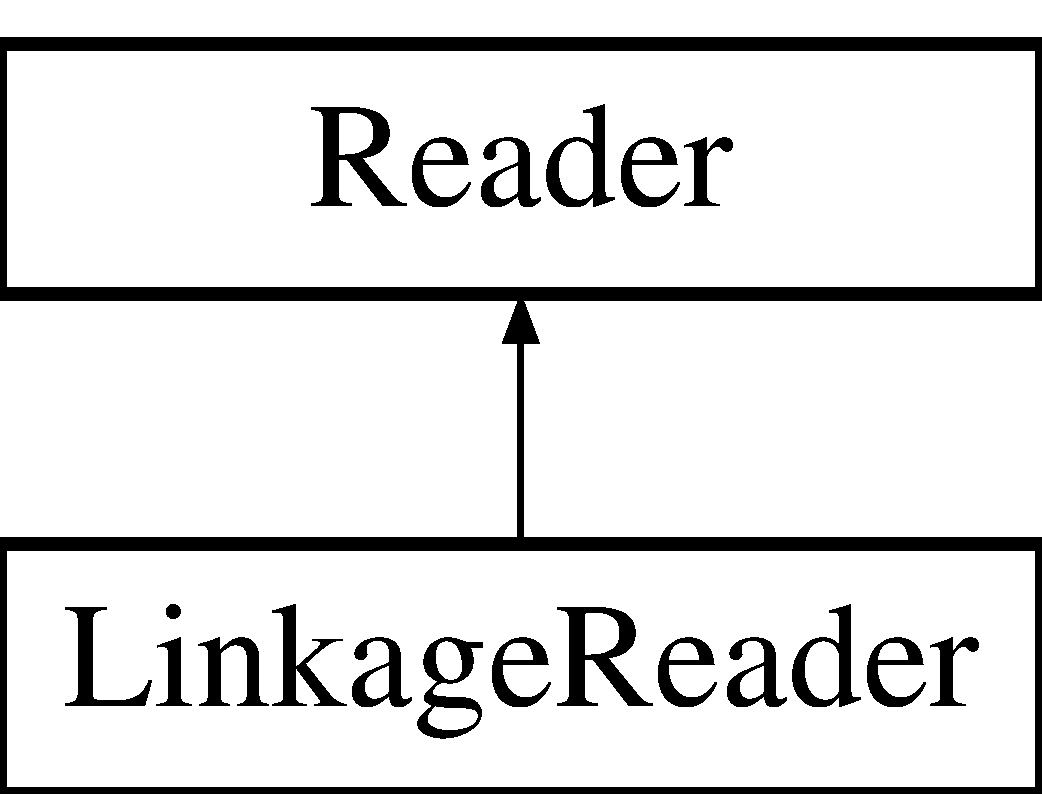
\includegraphics[height=2cm]{classLinkageReader}
\end{center}
\end{figure}
\subsection*{Public Member Functions}
\begin{DoxyCompactItemize}
\item 
\hyperlink{classLinkageReader_a2140f8868115116912be97afa7f970a5}{LinkageReader} ()
\item 
\hyperlink{classLinkageReader_a1422a6ab4deef5b8524ed24b90c4851b}{$\sim$LinkageReader} ()
\item 
virtual void \hyperlink{classLinkageReader_a808d3be4b0a2b3af8a7ec7fea963960b}{process} (\hyperlink{classSnpData}{SnpData} $\ast$, \hyperlink{classParamReader}{ParamReader} $\ast$)
\end{DoxyCompactItemize}


\subsection{Constructor \& Destructor Documentation}
\hypertarget{classLinkageReader_a2140f8868115116912be97afa7f970a5}{
\index{LinkageReader@{LinkageReader}!LinkageReader@{LinkageReader}}
\index{LinkageReader@{LinkageReader}!LinkageReader@{LinkageReader}}
\subsubsection[{LinkageReader}]{\setlength{\rightskip}{0pt plus 5cm}LinkageReader::LinkageReader ()}}
\label{classLinkageReader_a2140f8868115116912be97afa7f970a5}
\hypertarget{classLinkageReader_a1422a6ab4deef5b8524ed24b90c4851b}{
\index{LinkageReader@{LinkageReader}!$\sim$LinkageReader@{$\sim$LinkageReader}}
\index{$\sim$LinkageReader@{$\sim$LinkageReader}!LinkageReader@{LinkageReader}}
\subsubsection[{$\sim$LinkageReader}]{\setlength{\rightskip}{0pt plus 5cm}LinkageReader::$\sim$LinkageReader ()}}
\label{classLinkageReader_a1422a6ab4deef5b8524ed24b90c4851b}


\subsection{Member Function Documentation}
\hypertarget{classLinkageReader_a808d3be4b0a2b3af8a7ec7fea963960b}{
\index{LinkageReader@{LinkageReader}!process@{process}}
\index{process@{process}!LinkageReader@{LinkageReader}}
\subsubsection[{process}]{\setlength{\rightskip}{0pt plus 5cm}void LinkageReader::process ({\bf SnpData} $\ast$ {\em data}, \/  {\bf ParamReader} $\ast$ {\em params})\hspace{0.3cm}{\ttfamily  \mbox{[}virtual\mbox{]}}}}
\label{classLinkageReader_a808d3be4b0a2b3af8a7ec7fea963960b}
This is the entry point to any reader class. Will perform any necessary work to actually capture data.


\begin{DoxyParams}{Parameters}
\item[{\em data}]A \hyperlink{classSnpData}{SnpData} object that will hold the data we are collecting \item[{\em params}]A parameter object holding information about what to collect. \end{DoxyParams}


Implements \hyperlink{classReader_a334a724f607c84262af67759ffcdbd26}{Reader}.



The documentation for this class was generated from the following files:\begin{DoxyCompactItemize}
\item 
reader/\hyperlink{linkage__reader_8h}{linkage\_\-reader.h}\item 
reader/\hyperlink{linkage__reader_8cpp}{linkage\_\-reader.cpp}\end{DoxyCompactItemize}

\hypertarget{structLinRegStats}{
\section{LinRegStats Struct Reference}
\label{structLinRegStats}\index{LinRegStats@{LinRegStats}}
}


{\ttfamily \#include $<$linear\_\-regression.hh$>$}

\subsection*{Data Fields}
\begin{DoxyCompactItemize}
\item 
int \hyperlink{structLinRegStats_abcd9d1768c12d7f76fd2d840add86dd9}{i}
\end{DoxyCompactItemize}


\subsection{Field Documentation}
\hypertarget{structLinRegStats_abcd9d1768c12d7f76fd2d840add86dd9}{
\index{LinRegStats@{LinRegStats}!i@{i}}
\index{i@{i}!LinRegStats@{LinRegStats}}
\subsubsection[{i}]{\setlength{\rightskip}{0pt plus 5cm}int {\bf LinRegStats::i}}}
\label{structLinRegStats_abcd9d1768c12d7f76fd2d840add86dd9}


The documentation for this struct was generated from the following file:\begin{DoxyCompactItemize}
\item 
engine/utils/\hyperlink{linear__regression_8hh}{linear\_\-regression.hh}\end{DoxyCompactItemize}

\hypertarget{classLogger}{
\section{Logger Class Reference}
\label{classLogger}\index{Logger@{Logger}}
}


{\ttfamily \#include $<$log.hh$>$}

\subsection*{Public Member Functions}
\begin{DoxyCompactItemize}
\item 
bool \hyperlink{classLogger_af843738beb6818dedd7156a720141e98}{init} (string logFile)
\item 
void \hyperlink{classLogger_aa958f35a7eeb31a8ea4fff0c0574e029}{writeLine} (string line)
\item 
void \hyperlink{classLogger_afee2bab560c2db0190c980884d33868c}{close} ()
\end{DoxyCompactItemize}
\subsection*{Static Public Member Functions}
\begin{DoxyCompactItemize}
\item 
static \hyperlink{classLogger}{Logger} $\ast$ \hyperlink{classLogger_afae0bf19389387a916656073572cb846}{Instance} ()
\end{DoxyCompactItemize}


\subsection{Member Function Documentation}
\hypertarget{classLogger_afee2bab560c2db0190c980884d33868c}{
\index{Logger@{Logger}!close@{close}}
\index{close@{close}!Logger@{Logger}}
\subsubsection[{close}]{\setlength{\rightskip}{0pt plus 5cm}void Logger::close ()}}
\label{classLogger_afee2bab560c2db0190c980884d33868c}
\hypertarget{classLogger_af843738beb6818dedd7156a720141e98}{
\index{Logger@{Logger}!init@{init}}
\index{init@{init}!Logger@{Logger}}
\subsubsection[{init}]{\setlength{\rightskip}{0pt plus 5cm}bool Logger::init (string {\em logFile})}}
\label{classLogger_af843738beb6818dedd7156a720141e98}
\hypertarget{classLogger_afae0bf19389387a916656073572cb846}{
\index{Logger@{Logger}!Instance@{Instance}}
\index{Instance@{Instance}!Logger@{Logger}}
\subsubsection[{Instance}]{\setlength{\rightskip}{0pt plus 5cm}{\bf Logger} $\ast$ Logger::Instance ()\hspace{0.3cm}{\ttfamily  \mbox{[}static\mbox{]}}}}
\label{classLogger_afae0bf19389387a916656073572cb846}
This function is called to create an instance of the class. Calling the constructor publicly is not allowed. The constructor is private and is only called by this Instance function. \hypertarget{classLogger_aa958f35a7eeb31a8ea4fff0c0574e029}{
\index{Logger@{Logger}!writeLine@{writeLine}}
\index{writeLine@{writeLine}!Logger@{Logger}}
\subsubsection[{writeLine}]{\setlength{\rightskip}{0pt plus 5cm}void Logger::writeLine (string {\em line})}}
\label{classLogger_aa958f35a7eeb31a8ea4fff0c0574e029}


The documentation for this class was generated from the following files:\begin{DoxyCompactItemize}
\item 
logger/\hyperlink{log_8hh}{log.hh}\item 
logger/\hyperlink{log_8cpp}{log.cpp}\end{DoxyCompactItemize}

\hypertarget{classLogisticRegression}{
\section{LogisticRegression Class Reference}
\label{classLogisticRegression}\index{LogisticRegression@{LogisticRegression}}
}


{\ttfamily \#include $<$lr.hh$>$}

\subsection*{Public Member Functions}
\begin{DoxyCompactItemize}
\item 
\hyperlink{classLogisticRegression_ac052292dfeced0b7272e099e5ccb1dc3}{LogisticRegression} ()
\item 
\hyperlink{classLRStats}{LRStats} \hyperlink{classLogisticRegression_aae7d62475729b5b670759d24ea1a35ff}{getSingleStats} (const vector$<$ double $>$ \&betas, const vector$<$ vector$<$ double $>$ $>$ \&invInf, int index)
\item 
double \hyperlink{classLogisticRegression_a1dd5a75892af3383871e591c8ccb7905}{getStats} (const vector$<$ double $>$ \&betas, const vector$<$ vector$<$ double $>$ $>$ invInf, double \&chiS)
\item 
double \hyperlink{classLogisticRegression_a614dd5ad7eece3237edc37b56fced349}{likelihoodRatio} (const vector$<$ double $>$ \&betas1, const vector$<$ vector$<$ double $>$ $>$ \&data1, const vector$<$ double $>$ \&betas2, const vector$<$ vector$<$ double $>$ $>$ \&data2, const vector$<$ double $>$ phen)
\item 
vector$<$ double $>$ \hyperlink{classLogisticRegression_a8a7966506c2677d7426be408a7cb3f02}{expectedScores} (const vector$<$ double $>$ \&betas, const vector$<$ vector$<$ double $>$ $>$ \&data)
\item 
vector$<$ double $>$ \hyperlink{classLogisticRegression_a1724e4c7cc9a73db2712dbbbb9fbf204}{newtonRaphsonFast} (const vector$<$ vector$<$ double $>$ $>$ \&data, const vector$<$ double $>$ \&response, vector$<$ vector$<$ double $>$ $>$ \&invInfMatrix, double startVal=0.0)
\item 
vector$<$ double $>$ \hyperlink{classLogisticRegression_a298d29d0539412141a1e98205d1c4396}{newtonRaphson} (const vector$<$ vector$<$ double $>$ $>$ \&data, const vector$<$ double $>$ \&response, vector$<$ vector$<$ double $>$ $>$ \&invInfMatrix, double startVal=0.0)
\item 
bool \hyperlink{classLogisticRegression_ab61a51b6ca0816938b59bde88bc1082d}{invFisherInformation} (const vector$<$ vector$<$ double $>$ $>$ \&data, const vector$<$ double $>$ \&betas, vector$<$ vector$<$ double $>$ $>$ \&returnMatrix)
\item 
int \hyperlink{classLogisticRegression_a7de2efb78e07f9b46f34f8627fe8dae7}{dataIsSeparable} (const vector$<$ vector$<$ double $>$ $>$ \&data, const vector$<$ double $>$ \&response)
\end{DoxyCompactItemize}


\subsection{Detailed Description}
\begin{DoxyAuthor}{Author}
Richard T. Guy 
\end{DoxyAuthor}
\begin{DoxyDate}{Date}
July, 2010
\end{DoxyDate}
Logistic regression computation engine. 

\subsection{Constructor \& Destructor Documentation}
\hypertarget{classLogisticRegression_ac052292dfeced0b7272e099e5ccb1dc3}{
\index{LogisticRegression@{LogisticRegression}!LogisticRegression@{LogisticRegression}}
\index{LogisticRegression@{LogisticRegression}!LogisticRegression@{LogisticRegression}}
\subsubsection[{LogisticRegression}]{\setlength{\rightskip}{0pt plus 5cm}LogisticRegression::LogisticRegression ()}}
\label{classLogisticRegression_ac052292dfeced0b7272e099e5ccb1dc3}


\subsection{Member Function Documentation}
\hypertarget{classLogisticRegression_a7de2efb78e07f9b46f34f8627fe8dae7}{
\index{LogisticRegression@{LogisticRegression}!dataIsSeparable@{dataIsSeparable}}
\index{dataIsSeparable@{dataIsSeparable}!LogisticRegression@{LogisticRegression}}
\subsubsection[{dataIsSeparable}]{\setlength{\rightskip}{0pt plus 5cm}int LogisticRegression::dataIsSeparable (const vector$<$ vector$<$ double $>$ $>$ \& {\em data}, \/  const vector$<$ double $>$ \& {\em response})}}
\label{classLogisticRegression_a7de2efb78e07f9b46f34f8627fe8dae7}
Check whether any column in the data completely separates the response variable. If so, return the index. \hypertarget{classLogisticRegression_a8a7966506c2677d7426be408a7cb3f02}{
\index{LogisticRegression@{LogisticRegression}!expectedScores@{expectedScores}}
\index{expectedScores@{expectedScores}!LogisticRegression@{LogisticRegression}}
\subsubsection[{expectedScores}]{\setlength{\rightskip}{0pt plus 5cm}vector$<$ double $>$ LogisticRegression::expectedScores (const vector$<$ double $>$ \& {\em betas}, \/  const vector$<$ vector$<$ double $>$ $>$ \& {\em data})}}
\label{classLogisticRegression_a8a7966506c2677d7426be408a7cb3f02}
\hypertarget{classLogisticRegression_aae7d62475729b5b670759d24ea1a35ff}{
\index{LogisticRegression@{LogisticRegression}!getSingleStats@{getSingleStats}}
\index{getSingleStats@{getSingleStats}!LogisticRegression@{LogisticRegression}}
\subsubsection[{getSingleStats}]{\setlength{\rightskip}{0pt plus 5cm}{\bf LRStats} LogisticRegression::getSingleStats (const vector$<$ double $>$ \& {\em betas}, \/  const vector$<$ vector$<$ double $>$ $>$ \& {\em invInfMatrix}, \/  int {\em index})}}
\label{classLogisticRegression_aae7d62475729b5b670759d24ea1a35ff}
Compute p-\/value and SE.

P-\/value uses Z score. \hypertarget{classLogisticRegression_a1dd5a75892af3383871e591c8ccb7905}{
\index{LogisticRegression@{LogisticRegression}!getStats@{getStats}}
\index{getStats@{getStats}!LogisticRegression@{LogisticRegression}}
\subsubsection[{getStats}]{\setlength{\rightskip}{0pt plus 5cm}double LogisticRegression::getStats (const vector$<$ double $>$ \& {\em betas}, \/  const vector$<$ vector$<$ double $>$ $>$ {\em invInf}, \/  double \& {\em chiS})}}
\label{classLogisticRegression_a1dd5a75892af3383871e591c8ccb7905}
\hypertarget{classLogisticRegression_ab61a51b6ca0816938b59bde88bc1082d}{
\index{LogisticRegression@{LogisticRegression}!invFisherInformation@{invFisherInformation}}
\index{invFisherInformation@{invFisherInformation}!LogisticRegression@{LogisticRegression}}
\subsubsection[{invFisherInformation}]{\setlength{\rightskip}{0pt plus 5cm}bool LogisticRegression::invFisherInformation (const vector$<$ vector$<$ double $>$ $>$ \& {\em data}, \/  const vector$<$ double $>$ \& {\em betas}, \/  vector$<$ vector$<$ double $>$ $>$ \& {\em returnMatrix})}}
\label{classLogisticRegression_ab61a51b6ca0816938b59bde88bc1082d}
\hypertarget{classLogisticRegression_a614dd5ad7eece3237edc37b56fced349}{
\index{LogisticRegression@{LogisticRegression}!likelihoodRatio@{likelihoodRatio}}
\index{likelihoodRatio@{likelihoodRatio}!LogisticRegression@{LogisticRegression}}
\subsubsection[{likelihoodRatio}]{\setlength{\rightskip}{0pt plus 5cm}double LogisticRegression::likelihoodRatio (const vector$<$ double $>$ \& {\em betas1}, \/  const vector$<$ vector$<$ double $>$ $>$ \& {\em data1}, \/  const vector$<$ double $>$ \& {\em betas2}, \/  const vector$<$ vector$<$ double $>$ $>$ \& {\em data2}, \/  const vector$<$ double $>$ {\em phen})}}
\label{classLogisticRegression_a614dd5ad7eece3237edc37b56fced349}
Compute the likelhood ratio between null model (beta1) and non-\/null model (beta2)

D = -\/2 $\ast$ sum ( y\_\-i ln (pi\_\-i / y\_\-i) + (1 -\/ y\_\-i) ln ((1-\/pi\_\-i) / (1 -\/ y\_\-i) ) ) for given model pi.

Compute G = D model 1 -\/ D model 2

\begin{DoxyReturn}{Returns}
The likelihood statistic. 
\end{DoxyReturn}
\hypertarget{classLogisticRegression_a298d29d0539412141a1e98205d1c4396}{
\index{LogisticRegression@{LogisticRegression}!newtonRaphson@{newtonRaphson}}
\index{newtonRaphson@{newtonRaphson}!LogisticRegression@{LogisticRegression}}
\subsubsection[{newtonRaphson}]{\setlength{\rightskip}{0pt plus 5cm}vector$<$ double $>$ LogisticRegression::newtonRaphson (const vector$<$ vector$<$ double $>$ $>$ \& {\em data}, \/  const vector$<$ double $>$ \& {\em response}, \/  vector$<$ vector$<$ double $>$ $>$ \& {\em invInfMatrix}, \/  double {\em startVal} = {\ttfamily 0.0})}}
\label{classLogisticRegression_a298d29d0539412141a1e98205d1c4396}
\hypertarget{classLogisticRegression_a1724e4c7cc9a73db2712dbbbb9fbf204}{
\index{LogisticRegression@{LogisticRegression}!newtonRaphsonFast@{newtonRaphsonFast}}
\index{newtonRaphsonFast@{newtonRaphsonFast}!LogisticRegression@{LogisticRegression}}
\subsubsection[{newtonRaphsonFast}]{\setlength{\rightskip}{0pt plus 5cm}vector$<$ double $>$ LogisticRegression::newtonRaphsonFast (const vector$<$ vector$<$ double $>$ $>$ \& {\em data}, \/  const vector$<$ double $>$ \& {\em response}, \/  vector$<$ vector$<$ double $>$ $>$ \& {\em invInfMatrix}, \/  double {\em startVal} = {\ttfamily 0.0})}}
\label{classLogisticRegression_a1724e4c7cc9a73db2712dbbbb9fbf204}


The documentation for this class was generated from the following files:\begin{DoxyCompactItemize}
\item 
engine/utils/\hyperlink{lr_8hh}{lr.hh}\item 
engine/utils/\hyperlink{lr_8cpp}{lr.cpp}\end{DoxyCompactItemize}

\hypertarget{classLogisticRegressionException}{
\section{LogisticRegressionException Class Reference}
\label{classLogisticRegressionException}\index{LogisticRegressionException@{LogisticRegressionException}}
}


{\ttfamily \#include $<$exceptions.h$>$}

Inheritance diagram for LogisticRegressionException:\begin{figure}[H]
\begin{center}
\leavevmode
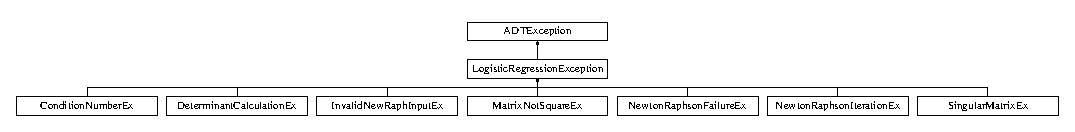
\includegraphics[height=1.32597cm]{classLogisticRegressionException}
\end{center}
\end{figure}


The documentation for this class was generated from the following file:\begin{DoxyCompactItemize}
\item 
engine/utils/\hyperlink{exceptions_8h}{exceptions.h}\end{DoxyCompactItemize}

\hypertarget{classLRStats}{
\section{LRStats Class Reference}
\label{classLRStats}\index{LRStats@{LRStats}}
}


{\ttfamily \#include $<$lr.hh$>$}

Inheritance diagram for LRStats:\begin{figure}[H]
\begin{center}
\leavevmode
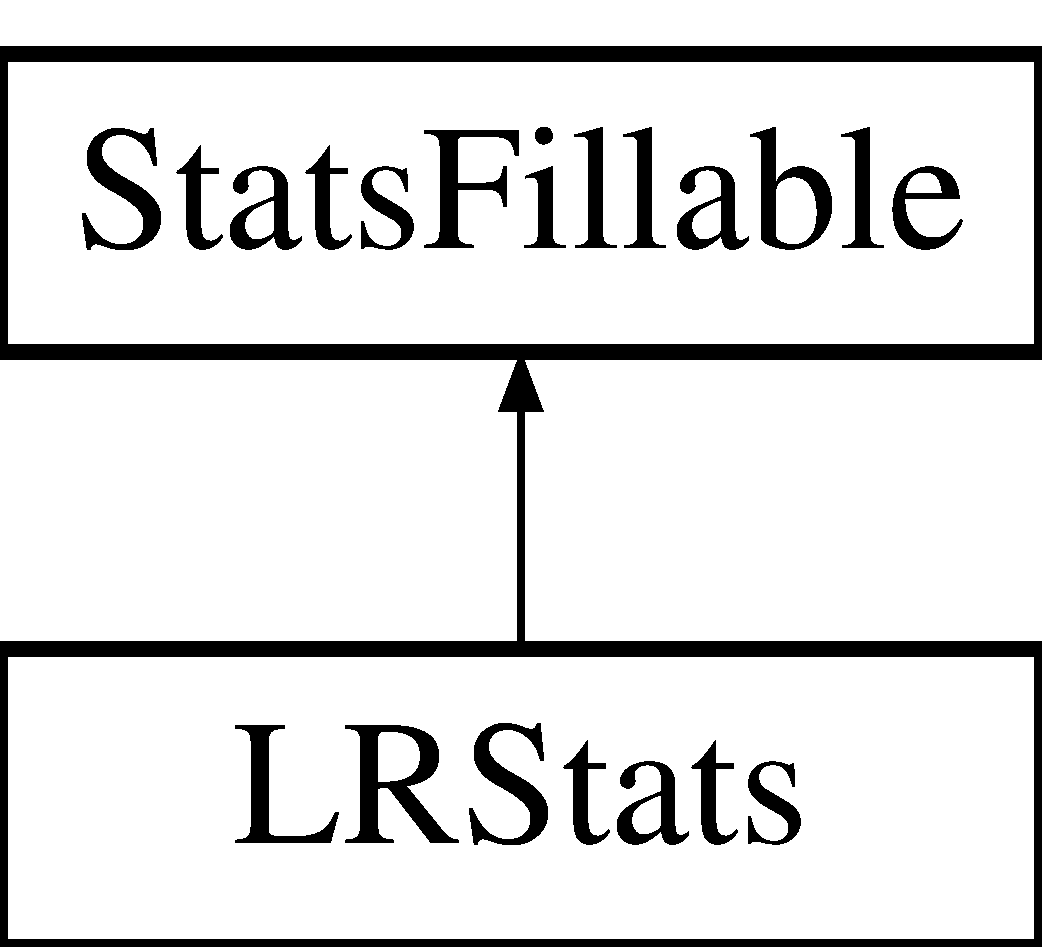
\includegraphics[height=2cm]{classLRStats}
\end{center}
\end{figure}
\subsection*{Public Member Functions}
\begin{DoxyCompactItemize}
\item 
void \hyperlink{classLRStats_a42f08be70d011bef6da77f20ffc999fe}{fillDefault} ()
\end{DoxyCompactItemize}
\subsection*{Data Fields}
\begin{DoxyCompactItemize}
\item 
double \hyperlink{classLRStats_ad2dc69ad8ef363196f7e1eb518d2749f}{OR}
\item 
double \hyperlink{classLRStats_a732a4d2d532d710c0eebbd55a5ea1cd4}{UCI}
\item 
double \hyperlink{classLRStats_a7a5645105fa178c1ae07ea41ce7265a7}{LCI}
\item 
double \hyperlink{classLRStats_a56946d63e769f7028683ce7899edd568}{testStat}
\item 
double \hyperlink{classLRStats_ab9c060dd747842d661d3ac3d3e7e7d8a}{pVal}
\item 
double \hyperlink{classLRStats_ad381b8b63712614b6d5cbdc46fdaf74f}{invInf}
\end{DoxyCompactItemize}


\subsection{Member Function Documentation}
\hypertarget{classLRStats_a42f08be70d011bef6da77f20ffc999fe}{
\index{LRStats@{LRStats}!fillDefault@{fillDefault}}
\index{fillDefault@{fillDefault}!LRStats@{LRStats}}
\subsubsection[{fillDefault}]{\setlength{\rightskip}{0pt plus 5cm}void LRStats::fillDefault ()\hspace{0.3cm}{\ttfamily  \mbox{[}inline, virtual\mbox{]}}}}
\label{classLRStats_a42f08be70d011bef6da77f20ffc999fe}


Implements \hyperlink{classStatsFillable_a6bc1a66ea949a078faa1b9ccdac54aba}{StatsFillable}.



\subsection{Field Documentation}
\hypertarget{classLRStats_ad381b8b63712614b6d5cbdc46fdaf74f}{
\index{LRStats@{LRStats}!invInf@{invInf}}
\index{invInf@{invInf}!LRStats@{LRStats}}
\subsubsection[{invInf}]{\setlength{\rightskip}{0pt plus 5cm}double {\bf LRStats::invInf}}}
\label{classLRStats_ad381b8b63712614b6d5cbdc46fdaf74f}
\hypertarget{classLRStats_a7a5645105fa178c1ae07ea41ce7265a7}{
\index{LRStats@{LRStats}!LCI@{LCI}}
\index{LCI@{LCI}!LRStats@{LRStats}}
\subsubsection[{LCI}]{\setlength{\rightskip}{0pt plus 5cm}double {\bf LRStats::LCI}}}
\label{classLRStats_a7a5645105fa178c1ae07ea41ce7265a7}
\hypertarget{classLRStats_ad2dc69ad8ef363196f7e1eb518d2749f}{
\index{LRStats@{LRStats}!OR@{OR}}
\index{OR@{OR}!LRStats@{LRStats}}
\subsubsection[{OR}]{\setlength{\rightskip}{0pt plus 5cm}double {\bf LRStats::OR}}}
\label{classLRStats_ad2dc69ad8ef363196f7e1eb518d2749f}
\hypertarget{classLRStats_ab9c060dd747842d661d3ac3d3e7e7d8a}{
\index{LRStats@{LRStats}!pVal@{pVal}}
\index{pVal@{pVal}!LRStats@{LRStats}}
\subsubsection[{pVal}]{\setlength{\rightskip}{0pt plus 5cm}double {\bf LRStats::pVal}}}
\label{classLRStats_ab9c060dd747842d661d3ac3d3e7e7d8a}
\hypertarget{classLRStats_a56946d63e769f7028683ce7899edd568}{
\index{LRStats@{LRStats}!testStat@{testStat}}
\index{testStat@{testStat}!LRStats@{LRStats}}
\subsubsection[{testStat}]{\setlength{\rightskip}{0pt plus 5cm}double {\bf LRStats::testStat}}}
\label{classLRStats_a56946d63e769f7028683ce7899edd568}
\hypertarget{classLRStats_a732a4d2d532d710c0eebbd55a5ea1cd4}{
\index{LRStats@{LRStats}!UCI@{UCI}}
\index{UCI@{UCI}!LRStats@{LRStats}}
\subsubsection[{UCI}]{\setlength{\rightskip}{0pt plus 5cm}double {\bf LRStats::UCI}}}
\label{classLRStats_a732a4d2d532d710c0eebbd55a5ea1cd4}


The documentation for this class was generated from the following file:\begin{DoxyCompactItemize}
\item 
engine/utils/\hyperlink{lr_8hh}{lr.hh}\end{DoxyCompactItemize}

\hypertarget{structSnpData_1_1MapData}{
\section{SnpData::MapData Struct Reference}
\label{structSnpData_1_1MapData}\index{SnpData::MapData@{SnpData::MapData}}
}


{\ttfamily \#include $<$snp\_\-data.hh$>$}

\subsection*{Data Fields}
\begin{DoxyCompactItemize}
\item 
long \hyperlink{structSnpData_1_1MapData_ac44edc4ea3bb6b526aa082eb19589f5b}{pos}
\item 
string \hyperlink{structSnpData_1_1MapData_a722c6b2849f9ce664afb172617fb4cbd}{chr}
\item 
string \hyperlink{structSnpData_1_1MapData_a75420d29bffd19b97db769f345f4b4ae}{name}
\item 
char \hyperlink{structSnpData_1_1MapData_af6f9c3ab44d69c3df9230d7076929a54}{refAllele}
\item 
bool \hyperlink{structSnpData_1_1MapData_aea06cd63b1801d2f4633f48fa42510b1}{flipped}
\end{DoxyCompactItemize}


\subsection{Field Documentation}
\hypertarget{structSnpData_1_1MapData_a722c6b2849f9ce664afb172617fb4cbd}{
\index{SnpData::MapData@{SnpData::MapData}!chr@{chr}}
\index{chr@{chr}!SnpData::MapData@{SnpData::MapData}}
\subsubsection[{chr}]{\setlength{\rightskip}{0pt plus 5cm}string {\bf SnpData::MapData::chr}}}
\label{structSnpData_1_1MapData_a722c6b2849f9ce664afb172617fb4cbd}
\hypertarget{structSnpData_1_1MapData_aea06cd63b1801d2f4633f48fa42510b1}{
\index{SnpData::MapData@{SnpData::MapData}!flipped@{flipped}}
\index{flipped@{flipped}!SnpData::MapData@{SnpData::MapData}}
\subsubsection[{flipped}]{\setlength{\rightskip}{0pt plus 5cm}bool {\bf SnpData::MapData::flipped}}}
\label{structSnpData_1_1MapData_aea06cd63b1801d2f4633f48fa42510b1}
\hypertarget{structSnpData_1_1MapData_a75420d29bffd19b97db769f345f4b4ae}{
\index{SnpData::MapData@{SnpData::MapData}!name@{name}}
\index{name@{name}!SnpData::MapData@{SnpData::MapData}}
\subsubsection[{name}]{\setlength{\rightskip}{0pt plus 5cm}string {\bf SnpData::MapData::name}}}
\label{structSnpData_1_1MapData_a75420d29bffd19b97db769f345f4b4ae}
\hypertarget{structSnpData_1_1MapData_ac44edc4ea3bb6b526aa082eb19589f5b}{
\index{SnpData::MapData@{SnpData::MapData}!pos@{pos}}
\index{pos@{pos}!SnpData::MapData@{SnpData::MapData}}
\subsubsection[{pos}]{\setlength{\rightskip}{0pt plus 5cm}long {\bf SnpData::MapData::pos}}}
\label{structSnpData_1_1MapData_ac44edc4ea3bb6b526aa082eb19589f5b}
\hypertarget{structSnpData_1_1MapData_af6f9c3ab44d69c3df9230d7076929a54}{
\index{SnpData::MapData@{SnpData::MapData}!refAllele@{refAllele}}
\index{refAllele@{refAllele}!SnpData::MapData@{SnpData::MapData}}
\subsubsection[{refAllele}]{\setlength{\rightskip}{0pt plus 5cm}char {\bf SnpData::MapData::refAllele}}}
\label{structSnpData_1_1MapData_af6f9c3ab44d69c3df9230d7076929a54}


The documentation for this struct was generated from the following file:\begin{DoxyCompactItemize}
\item 
engine/\hyperlink{snp__data_8hh}{snp\_\-data.hh}\end{DoxyCompactItemize}

\hypertarget{structMapData}{
\section{MapData Struct Reference}
\label{structMapData}\index{MapData@{MapData}}
}
\subsection*{Data Fields}
\begin{DoxyCompactItemize}
\item 
long \hyperlink{structMapData_a39c0ddcd241418ae2cb9c768e542b16f}{pos}
\item 
string \hyperlink{structMapData_a3d422e5b31b80cc7c4538a68af566574}{chr}
\item 
string \hyperlink{structMapData_ad4f885d78b08c2cf7bab7b75a014eb94}{name}
\item 
char \hyperlink{structMapData_a26658a6770ee7316368ebcaaf6d9e9e5}{refAllele}
\item 
bool \hyperlink{structMapData_a72b529932979ffbcda46669cb342a4c8}{flipped}
\end{DoxyCompactItemize}


\subsection{Field Documentation}
\hypertarget{structMapData_a3d422e5b31b80cc7c4538a68af566574}{
\index{MapData@{MapData}!chr@{chr}}
\index{chr@{chr}!MapData@{MapData}}
\subsubsection[{chr}]{\setlength{\rightskip}{0pt plus 5cm}string {\bf MapData::chr}}}
\label{structMapData_a3d422e5b31b80cc7c4538a68af566574}
\hypertarget{structMapData_a72b529932979ffbcda46669cb342a4c8}{
\index{MapData@{MapData}!flipped@{flipped}}
\index{flipped@{flipped}!MapData@{MapData}}
\subsubsection[{flipped}]{\setlength{\rightskip}{0pt plus 5cm}bool {\bf MapData::flipped}}}
\label{structMapData_a72b529932979ffbcda46669cb342a4c8}
\hypertarget{structMapData_ad4f885d78b08c2cf7bab7b75a014eb94}{
\index{MapData@{MapData}!name@{name}}
\index{name@{name}!MapData@{MapData}}
\subsubsection[{name}]{\setlength{\rightskip}{0pt plus 5cm}string {\bf MapData::name}}}
\label{structMapData_ad4f885d78b08c2cf7bab7b75a014eb94}
\hypertarget{structMapData_a39c0ddcd241418ae2cb9c768e542b16f}{
\index{MapData@{MapData}!pos@{pos}}
\index{pos@{pos}!MapData@{MapData}}
\subsubsection[{pos}]{\setlength{\rightskip}{0pt plus 5cm}long {\bf MapData::pos}}}
\label{structMapData_a39c0ddcd241418ae2cb9c768e542b16f}
\hypertarget{structMapData_a26658a6770ee7316368ebcaaf6d9e9e5}{
\index{MapData@{MapData}!refAllele@{refAllele}}
\index{refAllele@{refAllele}!MapData@{MapData}}
\subsubsection[{refAllele}]{\setlength{\rightskip}{0pt plus 5cm}char {\bf MapData::refAllele}}}
\label{structMapData_a26658a6770ee7316368ebcaaf6d9e9e5}


The documentation for this struct was generated from the following file:\begin{DoxyCompactItemize}
\item 
reader/\hyperlink{binary__bed__reader_8cpp}{binary\_\-bed\_\-reader.cpp}\end{DoxyCompactItemize}

\hypertarget{classMatrixNotSquareEx}{
\section{MatrixNotSquareEx Class Reference}
\label{classMatrixNotSquareEx}\index{MatrixNotSquareEx@{MatrixNotSquareEx}}
}


{\ttfamily \#include $<$exceptions.h$>$}

Inheritance diagram for MatrixNotSquareEx:\begin{figure}[H]
\begin{center}
\leavevmode
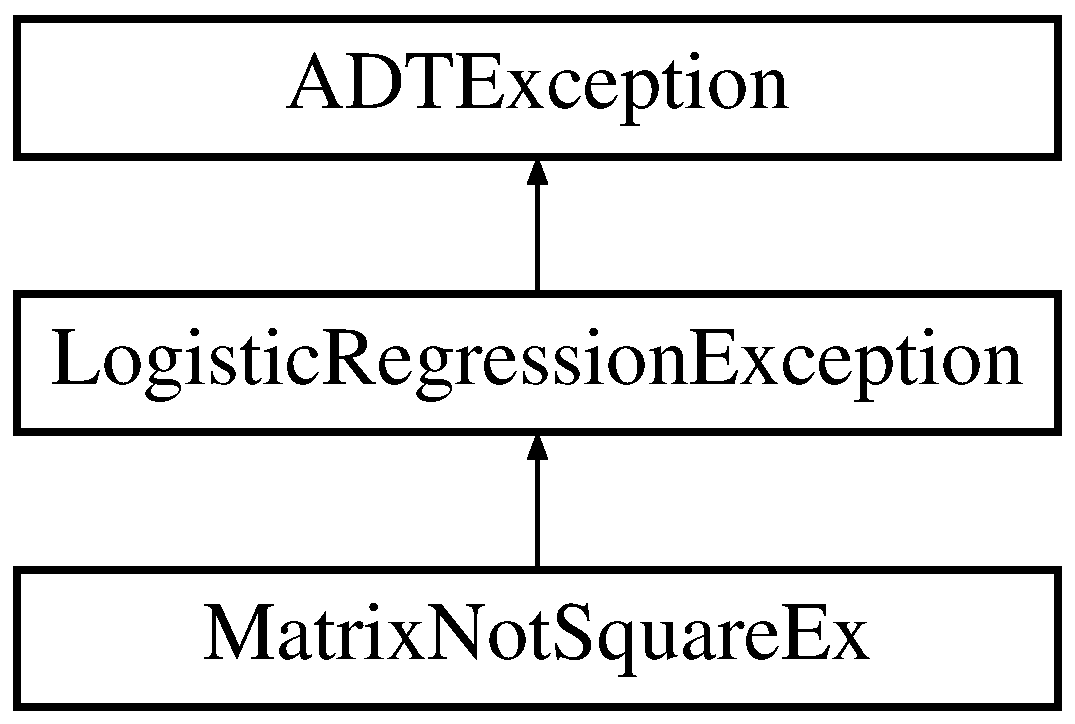
\includegraphics[height=3cm]{classMatrixNotSquareEx}
\end{center}
\end{figure}


The documentation for this class was generated from the following file:\begin{DoxyCompactItemize}
\item 
engine/utils/\hyperlink{exceptions_8h}{exceptions.h}\end{DoxyCompactItemize}

\hypertarget{classNewtonRaphsonFailureEx}{
\section{NewtonRaphsonFailureEx Class Reference}
\label{classNewtonRaphsonFailureEx}\index{NewtonRaphsonFailureEx@{NewtonRaphsonFailureEx}}
}


{\ttfamily \#include $<$exceptions.h$>$}

Inheritance diagram for NewtonRaphsonFailureEx:\begin{figure}[H]
\begin{center}
\leavevmode
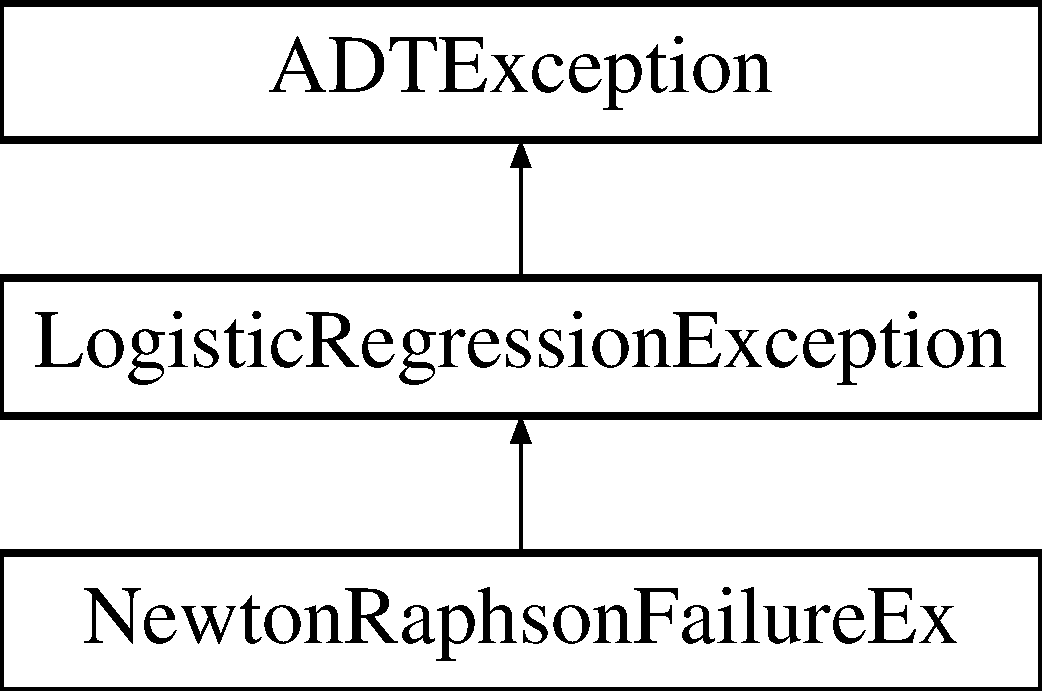
\includegraphics[height=3cm]{classNewtonRaphsonFailureEx}
\end{center}
\end{figure}


The documentation for this class was generated from the following file:\begin{DoxyCompactItemize}
\item 
engine/utils/\hyperlink{exceptions_8h}{exceptions.h}\end{DoxyCompactItemize}

\hypertarget{classNewtonRaphsonIterationEx}{
\section{NewtonRaphsonIterationEx Class Reference}
\label{classNewtonRaphsonIterationEx}\index{NewtonRaphsonIterationEx@{NewtonRaphsonIterationEx}}
}


{\ttfamily \#include $<$exceptions.h$>$}

Inheritance diagram for NewtonRaphsonIterationEx:\begin{figure}[H]
\begin{center}
\leavevmode
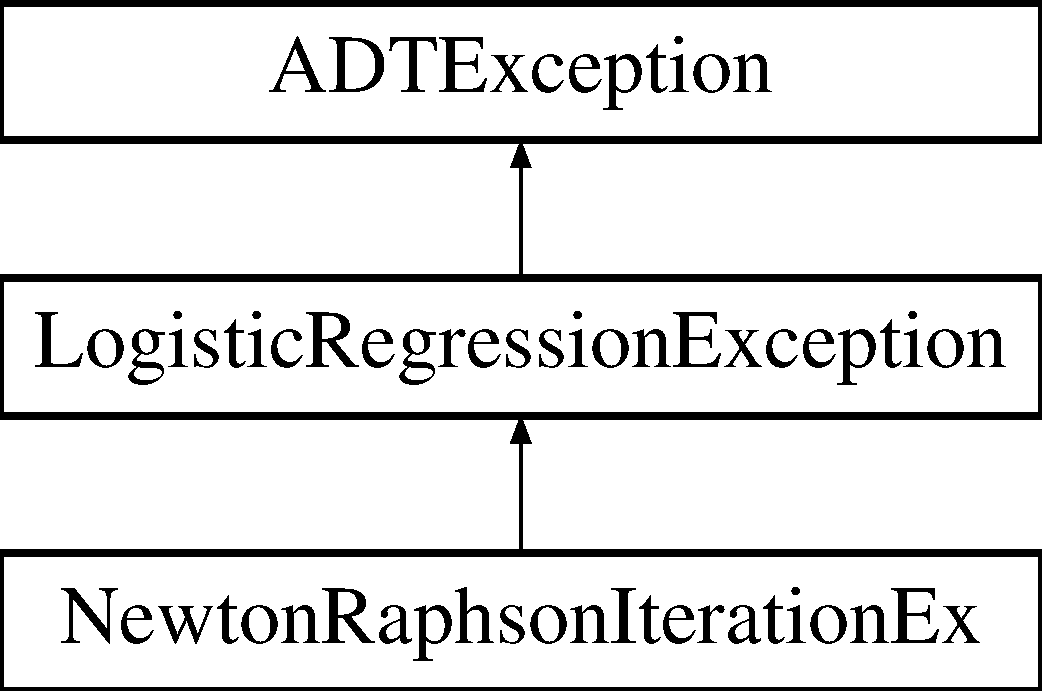
\includegraphics[height=3cm]{classNewtonRaphsonIterationEx}
\end{center}
\end{figure}


The documentation for this class was generated from the following file:\begin{DoxyCompactItemize}
\item 
engine/utils/\hyperlink{exceptions_8h}{exceptions.h}\end{DoxyCompactItemize}

\hypertarget{classOutput}{
\section{Output Class Reference}
\label{classOutput}\index{Output@{Output}}
}


{\ttfamily \#include $<$output.h$>$}

\subsection*{Public Member Functions}
\begin{DoxyCompactItemize}
\item 
\hyperlink{classOutput_a428c663520336477a12f1a33504eb067}{Output} ()
\item 
bool \hyperlink{classOutput_a5622f8a5844d8a705d16c91abe4e3fa3}{init} (string fileName)
\item 
void \hyperlink{classOutput_a8ad983d5d1526a180e3a9cdb005b4198}{close} ()
\item 
void \hyperlink{classOutput_a0e201407bdd9555b8618575ce155ca20}{flush} ()
\item 
void \hyperlink{classOutput_ac8c48b57590c89dcd7993c8497ddde23}{write\_\-header} (string head)
\item 
void \hyperlink{classOutput_a616ea937fe1d9b04fcd60cbd4797e3c4}{write\_\-line} (string line, int order)
\end{DoxyCompactItemize}


\subsection{Constructor \& Destructor Documentation}
\hypertarget{classOutput_a428c663520336477a12f1a33504eb067}{
\index{Output@{Output}!Output@{Output}}
\index{Output@{Output}!Output@{Output}}
\subsubsection[{Output}]{\setlength{\rightskip}{0pt plus 5cm}Output::Output ()}}
\label{classOutput_a428c663520336477a12f1a33504eb067}


\subsection{Member Function Documentation}
\hypertarget{classOutput_a8ad983d5d1526a180e3a9cdb005b4198}{
\index{Output@{Output}!close@{close}}
\index{close@{close}!Output@{Output}}
\subsubsection[{close}]{\setlength{\rightskip}{0pt plus 5cm}void Output::close ()}}
\label{classOutput_a8ad983d5d1526a180e3a9cdb005b4198}
\hypertarget{classOutput_a0e201407bdd9555b8618575ce155ca20}{
\index{Output@{Output}!flush@{flush}}
\index{flush@{flush}!Output@{Output}}
\subsubsection[{flush}]{\setlength{\rightskip}{0pt plus 5cm}void Output::flush ()}}
\label{classOutput_a0e201407bdd9555b8618575ce155ca20}
\hypertarget{classOutput_a5622f8a5844d8a705d16c91abe4e3fa3}{
\index{Output@{Output}!init@{init}}
\index{init@{init}!Output@{Output}}
\subsubsection[{init}]{\setlength{\rightskip}{0pt plus 5cm}bool Output::init (string {\em fileName})}}
\label{classOutput_a5622f8a5844d8a705d16c91abe4e3fa3}
\hypertarget{classOutput_ac8c48b57590c89dcd7993c8497ddde23}{
\index{Output@{Output}!write\_\-header@{write\_\-header}}
\index{write\_\-header@{write\_\-header}!Output@{Output}}
\subsubsection[{write\_\-header}]{\setlength{\rightskip}{0pt plus 5cm}void Output::write\_\-header (string {\em head})}}
\label{classOutput_ac8c48b57590c89dcd7993c8497ddde23}
\hypertarget{classOutput_a616ea937fe1d9b04fcd60cbd4797e3c4}{
\index{Output@{Output}!write\_\-line@{write\_\-line}}
\index{write\_\-line@{write\_\-line}!Output@{Output}}
\subsubsection[{write\_\-line}]{\setlength{\rightskip}{0pt plus 5cm}void Output::write\_\-line (string {\em line}, \/  int {\em order})}}
\label{classOutput_a616ea937fe1d9b04fcd60cbd4797e3c4}


The documentation for this class was generated from the following files:\begin{DoxyCompactItemize}
\item 
engine/output/\hyperlink{output_8h}{output.h}\item 
engine/output/\hyperlink{output_8cpp}{output.cpp}\end{DoxyCompactItemize}

\hypertarget{classParamReader}{
\section{ParamReader Class Reference}
\label{classParamReader}\index{ParamReader@{ParamReader}}
}


{\ttfamily \#include $<$param\_\-reader.h$>$}

\subsection*{Public Types}
\begin{DoxyCompactItemize}
\item 
enum \hyperlink{classParamReader_a5954b9845fceb081c5e259dfc7118238}{InputTypes} \{ \hyperlink{classParamReader_a5954b9845fceb081c5e259dfc7118238a7375bfa42146fea4290360622fc5345e}{ARFF}, 
\hyperlink{classParamReader_a5954b9845fceb081c5e259dfc7118238ad72ac83343e74998040fdebd70c05284}{LINKAGE}
 \}
\item 
enum \hyperlink{classParamReader_ade771142042ad0251f905f38248ae9df}{EngineTypes} \{ \par
\hyperlink{classParamReader_ade771142042ad0251f905f38248ae9dfa4f93cf77f6a672cb915b25005ad3842e}{UNASSIGNED}, 
\hyperlink{classParamReader_ade771142042ad0251f905f38248ae9dfa9413313d32f2792b15708e6768f1f80b}{BAGGING}, 
\hyperlink{classParamReader_ade771142042ad0251f905f38248ae9dfa21e66dd9f5fceffaa9c7e22e1fbd8a65}{ADTREE}, 
\hyperlink{classParamReader_ade771142042ad0251f905f38248ae9dfa0a2f7bd0340be5eb2db7727af93a035b}{SNPGWA}, 
\par
\hyperlink{classParamReader_ade771142042ad0251f905f38248ae9dfa87d48919f03f8f6e437af98d73ce0554}{FORMAT}, 
\hyperlink{classParamReader_ade771142042ad0251f905f38248ae9dfad44bbb13488be83b446edf2f1698400d}{CROSSVAL}, 
\hyperlink{classParamReader_ade771142042ad0251f905f38248ae9dfa6f24418bf4d9982f3e02a4bf9aa43698}{DPRIME}, 
\hyperlink{classParamReader_ade771142042ad0251f905f38248ae9dfa261db4ce98a8183ce7d42feae1ca097d}{QSNPGWA}, 
\par
\hyperlink{classParamReader_ade771142042ad0251f905f38248ae9dfa4c66f07e11e6044f872c6971243ee714}{DANDELION}, 
\hyperlink{classParamReader_ade771142042ad0251f905f38248ae9dfacc516636ab57343817a97a8e822a4f62}{INTERTWOLOG}
 \}
\end{DoxyCompactItemize}
\subsection*{Public Member Functions}
\begin{DoxyCompactItemize}
\item 
bool \hyperlink{classParamReader_aeccf4ded55394619359a2c85bc163b57}{process\_\-parameters} (int argc, char $\ast$argv\mbox{[}$\,$\mbox{]})
\item 
bool \hyperlink{classParamReader_a3b1cf53fc0ed5ffd32744852f7c0015d}{use\_\-this} (int i)
\begin{DoxyCompactList}\small\item\em Skip related function. \item\end{DoxyCompactList}\item 
bool \hyperlink{classParamReader_ab3a203d5c9698bf8ed1bcd7b7d77a263}{in\_\-window} (int i)
\begin{DoxyCompactList}\small\item\em Windowing function. \item\end{DoxyCompactList}\item 
string \hyperlink{classParamReader_a3fbb431f095c3eec170925a2e694c906}{get\_\-linkage\_\-geno\_\-file} ()
\begin{DoxyCompactList}\small\item\em Keep all parameters private and use getter/setters. \item\end{DoxyCompactList}\item 
string \hyperlink{classParamReader_a10a774de006ca94c081a960e60067673}{get\_\-linkage\_\-pheno\_\-file} ()
\item 
string \hyperlink{classParamReader_a0ad3f8e7cecb2a30b68894da7ae60986}{get\_\-linkage\_\-map\_\-file} ()
\item 
string \hyperlink{classParamReader_a1db0df02a87cf08451a306fe64687dda}{get\_\-arff\_\-file} ()
\item 
string \hyperlink{classParamReader_a37437fb7b8c52a7b0d820aa12368adfd}{get\_\-out\_\-file} ()
\item 
string \hyperlink{classParamReader_ae45f59e58362073c2f957feb11267a75}{get\_\-log\_\-file} ()
\item 
int \hyperlink{classParamReader_a61dd4ab6c8ad46531fb55c138f59c296}{get\_\-verbosity} ()
\item 
string \hyperlink{classParamReader_ab630108daee4ef506b82e6ecc61f0852}{get\_\-trait} ()
\item 
bool \hyperlink{classParamReader_a288cde2c7b78f3ffeb28e9d56a595826}{get\_\-ign} ()
\item 
vector$<$ string $>$ \hyperlink{classParamReader_a24781bbe8138d3c4eedb072ce88f5b95}{get\_\-covariates} ()
\item 
int \hyperlink{classParamReader_acbc52d902d67738b096a0b41bcf7d61d}{get\_\-begin} ()
\item 
int \hyperlink{classParamReader_a7f97caf26c9a65a6634b66f27d48f258}{get\_\-end} ()
\item 
int \hyperlink{classParamReader_a49f7db5405ebe1a3c61dadcfac296d49}{get\_\-win} ()
\item 
vector$<$ string $>$ $\ast$ \hyperlink{classParamReader_aa92383f88df295288d31a154c35a43ab}{get\_\-engine\_\-specific\_\-params} ()
\item 
\hyperlink{classParamReader_a5954b9845fceb081c5e259dfc7118238}{InputTypes} \hyperlink{classParamReader_ad2e79ce88de8894f58b38f6ff6452b02}{get\_\-input\_\-type} ()
\item 
\hyperlink{classParamReader_ade771142042ad0251f905f38248ae9df}{EngineTypes} \hyperlink{classParamReader_a2a0885d0793cc84eeaf641f5b36d6fae}{get\_\-engine\_\-types} ()
\end{DoxyCompactItemize}
\subsection*{Static Public Member Functions}
\begin{DoxyCompactItemize}
\item 
static \hyperlink{classParamReader}{ParamReader} $\ast$ \hyperlink{classParamReader_a418f7d1f1bf0ad4cb3a6e7aaccc9ead3}{Instance} ()
\end{DoxyCompactItemize}


\subsection{Detailed Description}
General parameter reader. Two sets of parameters exist for this program.

\hyperlink{classEngine}{Engine} specific would have a -\/-\/ start. General will have a -\/ start. This class handles all -\/ parameters and passes -\/-\/ on.

Available parameters: Linkage file format (mutually exclusive with arff format.) -\/geno $<$file$>$ -\/phen $<$file$>$ -\/map $<$file$>$ Arff format -\/arff $<$file$>$ \hyperlink{classEngine}{Engine} specification: -\/engine $<$adtree $|$ bagging$>$

Windowing parameters: -\/beg $<$int$>$ -\/end $<$int$>$ paired -\/win $<$int$>$ alone. (two are exclusive)

-\/skip $<$cols$>$ 

\subsection{Member Enumeration Documentation}
\hypertarget{classParamReader_ade771142042ad0251f905f38248ae9df}{
\index{ParamReader@{ParamReader}!EngineTypes@{EngineTypes}}
\index{EngineTypes@{EngineTypes}!ParamReader@{ParamReader}}
\subsubsection[{EngineTypes}]{\setlength{\rightskip}{0pt plus 5cm}enum {\bf ParamReader::EngineTypes}}}
\label{classParamReader_ade771142042ad0251f905f38248ae9df}
\begin{Desc}
\item[Enumerator: ]\par
\begin{description}
\index{UNASSIGNED@{UNASSIGNED}!ParamReader@{ParamReader}}\index{ParamReader@{ParamReader}!UNASSIGNED@{UNASSIGNED}}\item[{\em 
\hypertarget{classParamReader_ade771142042ad0251f905f38248ae9dfa4f93cf77f6a672cb915b25005ad3842e}{
UNASSIGNED}
\label{classParamReader_ade771142042ad0251f905f38248ae9dfa4f93cf77f6a672cb915b25005ad3842e}
}]\index{BAGGING@{BAGGING}!ParamReader@{ParamReader}}\index{ParamReader@{ParamReader}!BAGGING@{BAGGING}}\item[{\em 
\hypertarget{classParamReader_ade771142042ad0251f905f38248ae9dfa9413313d32f2792b15708e6768f1f80b}{
BAGGING}
\label{classParamReader_ade771142042ad0251f905f38248ae9dfa9413313d32f2792b15708e6768f1f80b}
}]\index{ADTREE@{ADTREE}!ParamReader@{ParamReader}}\index{ParamReader@{ParamReader}!ADTREE@{ADTREE}}\item[{\em 
\hypertarget{classParamReader_ade771142042ad0251f905f38248ae9dfa21e66dd9f5fceffaa9c7e22e1fbd8a65}{
ADTREE}
\label{classParamReader_ade771142042ad0251f905f38248ae9dfa21e66dd9f5fceffaa9c7e22e1fbd8a65}
}]\index{SNPGWA@{SNPGWA}!ParamReader@{ParamReader}}\index{ParamReader@{ParamReader}!SNPGWA@{SNPGWA}}\item[{\em 
\hypertarget{classParamReader_ade771142042ad0251f905f38248ae9dfa0a2f7bd0340be5eb2db7727af93a035b}{
SNPGWA}
\label{classParamReader_ade771142042ad0251f905f38248ae9dfa0a2f7bd0340be5eb2db7727af93a035b}
}]\index{FORMAT@{FORMAT}!ParamReader@{ParamReader}}\index{ParamReader@{ParamReader}!FORMAT@{FORMAT}}\item[{\em 
\hypertarget{classParamReader_ade771142042ad0251f905f38248ae9dfa87d48919f03f8f6e437af98d73ce0554}{
FORMAT}
\label{classParamReader_ade771142042ad0251f905f38248ae9dfa87d48919f03f8f6e437af98d73ce0554}
}]\index{CROSSVAL@{CROSSVAL}!ParamReader@{ParamReader}}\index{ParamReader@{ParamReader}!CROSSVAL@{CROSSVAL}}\item[{\em 
\hypertarget{classParamReader_ade771142042ad0251f905f38248ae9dfad44bbb13488be83b446edf2f1698400d}{
CROSSVAL}
\label{classParamReader_ade771142042ad0251f905f38248ae9dfad44bbb13488be83b446edf2f1698400d}
}]\index{DPRIME@{DPRIME}!ParamReader@{ParamReader}}\index{ParamReader@{ParamReader}!DPRIME@{DPRIME}}\item[{\em 
\hypertarget{classParamReader_ade771142042ad0251f905f38248ae9dfa6f24418bf4d9982f3e02a4bf9aa43698}{
DPRIME}
\label{classParamReader_ade771142042ad0251f905f38248ae9dfa6f24418bf4d9982f3e02a4bf9aa43698}
}]\index{QSNPGWA@{QSNPGWA}!ParamReader@{ParamReader}}\index{ParamReader@{ParamReader}!QSNPGWA@{QSNPGWA}}\item[{\em 
\hypertarget{classParamReader_ade771142042ad0251f905f38248ae9dfa261db4ce98a8183ce7d42feae1ca097d}{
QSNPGWA}
\label{classParamReader_ade771142042ad0251f905f38248ae9dfa261db4ce98a8183ce7d42feae1ca097d}
}]\index{DANDELION@{DANDELION}!ParamReader@{ParamReader}}\index{ParamReader@{ParamReader}!DANDELION@{DANDELION}}\item[{\em 
\hypertarget{classParamReader_ade771142042ad0251f905f38248ae9dfa4c66f07e11e6044f872c6971243ee714}{
DANDELION}
\label{classParamReader_ade771142042ad0251f905f38248ae9dfa4c66f07e11e6044f872c6971243ee714}
}]\index{INTERTWOLOG@{INTERTWOLOG}!ParamReader@{ParamReader}}\index{ParamReader@{ParamReader}!INTERTWOLOG@{INTERTWOLOG}}\item[{\em 
\hypertarget{classParamReader_ade771142042ad0251f905f38248ae9dfacc516636ab57343817a97a8e822a4f62}{
INTERTWOLOG}
\label{classParamReader_ade771142042ad0251f905f38248ae9dfacc516636ab57343817a97a8e822a4f62}
}]\end{description}
\end{Desc}

\hypertarget{classParamReader_a5954b9845fceb081c5e259dfc7118238}{
\index{ParamReader@{ParamReader}!InputTypes@{InputTypes}}
\index{InputTypes@{InputTypes}!ParamReader@{ParamReader}}
\subsubsection[{InputTypes}]{\setlength{\rightskip}{0pt plus 5cm}enum {\bf ParamReader::InputTypes}}}
\label{classParamReader_a5954b9845fceb081c5e259dfc7118238}
\begin{Desc}
\item[Enumerator: ]\par
\begin{description}
\index{ARFF@{ARFF}!ParamReader@{ParamReader}}\index{ParamReader@{ParamReader}!ARFF@{ARFF}}\item[{\em 
\hypertarget{classParamReader_a5954b9845fceb081c5e259dfc7118238a7375bfa42146fea4290360622fc5345e}{
ARFF}
\label{classParamReader_a5954b9845fceb081c5e259dfc7118238a7375bfa42146fea4290360622fc5345e}
}]\index{LINKAGE@{LINKAGE}!ParamReader@{ParamReader}}\index{ParamReader@{ParamReader}!LINKAGE@{LINKAGE}}\item[{\em 
\hypertarget{classParamReader_a5954b9845fceb081c5e259dfc7118238ad72ac83343e74998040fdebd70c05284}{
LINKAGE}
\label{classParamReader_a5954b9845fceb081c5e259dfc7118238ad72ac83343e74998040fdebd70c05284}
}]\end{description}
\end{Desc}



\subsection{Member Function Documentation}
\hypertarget{classParamReader_a1db0df02a87cf08451a306fe64687dda}{
\index{ParamReader@{ParamReader}!get\_\-arff\_\-file@{get\_\-arff\_\-file}}
\index{get\_\-arff\_\-file@{get\_\-arff\_\-file}!ParamReader@{ParamReader}}
\subsubsection[{get\_\-arff\_\-file}]{\setlength{\rightskip}{0pt plus 5cm}string ParamReader::get\_\-arff\_\-file ()\hspace{0.3cm}{\ttfamily  \mbox{[}inline\mbox{]}}}}
\label{classParamReader_a1db0df02a87cf08451a306fe64687dda}
\hypertarget{classParamReader_acbc52d902d67738b096a0b41bcf7d61d}{
\index{ParamReader@{ParamReader}!get\_\-begin@{get\_\-begin}}
\index{get\_\-begin@{get\_\-begin}!ParamReader@{ParamReader}}
\subsubsection[{get\_\-begin}]{\setlength{\rightskip}{0pt plus 5cm}int ParamReader::get\_\-begin ()\hspace{0.3cm}{\ttfamily  \mbox{[}inline\mbox{]}}}}
\label{classParamReader_acbc52d902d67738b096a0b41bcf7d61d}
\hypertarget{classParamReader_a24781bbe8138d3c4eedb072ce88f5b95}{
\index{ParamReader@{ParamReader}!get\_\-covariates@{get\_\-covariates}}
\index{get\_\-covariates@{get\_\-covariates}!ParamReader@{ParamReader}}
\subsubsection[{get\_\-covariates}]{\setlength{\rightskip}{0pt plus 5cm}vector$<$string$>$ ParamReader::get\_\-covariates ()\hspace{0.3cm}{\ttfamily  \mbox{[}inline\mbox{]}}}}
\label{classParamReader_a24781bbe8138d3c4eedb072ce88f5b95}
\hypertarget{classParamReader_a7f97caf26c9a65a6634b66f27d48f258}{
\index{ParamReader@{ParamReader}!get\_\-end@{get\_\-end}}
\index{get\_\-end@{get\_\-end}!ParamReader@{ParamReader}}
\subsubsection[{get\_\-end}]{\setlength{\rightskip}{0pt plus 5cm}int ParamReader::get\_\-end ()\hspace{0.3cm}{\ttfamily  \mbox{[}inline\mbox{]}}}}
\label{classParamReader_a7f97caf26c9a65a6634b66f27d48f258}
\hypertarget{classParamReader_aa92383f88df295288d31a154c35a43ab}{
\index{ParamReader@{ParamReader}!get\_\-engine\_\-specific\_\-params@{get\_\-engine\_\-specific\_\-params}}
\index{get\_\-engine\_\-specific\_\-params@{get\_\-engine\_\-specific\_\-params}!ParamReader@{ParamReader}}
\subsubsection[{get\_\-engine\_\-specific\_\-params}]{\setlength{\rightskip}{0pt plus 5cm}vector$<$string$>$$\ast$ ParamReader::get\_\-engine\_\-specific\_\-params ()\hspace{0.3cm}{\ttfamily  \mbox{[}inline\mbox{]}}}}
\label{classParamReader_aa92383f88df295288d31a154c35a43ab}
\hypertarget{classParamReader_a2a0885d0793cc84eeaf641f5b36d6fae}{
\index{ParamReader@{ParamReader}!get\_\-engine\_\-types@{get\_\-engine\_\-types}}
\index{get\_\-engine\_\-types@{get\_\-engine\_\-types}!ParamReader@{ParamReader}}
\subsubsection[{get\_\-engine\_\-types}]{\setlength{\rightskip}{0pt plus 5cm}{\bf EngineTypes} ParamReader::get\_\-engine\_\-types ()\hspace{0.3cm}{\ttfamily  \mbox{[}inline\mbox{]}}}}
\label{classParamReader_a2a0885d0793cc84eeaf641f5b36d6fae}
\hypertarget{classParamReader_a288cde2c7b78f3ffeb28e9d56a595826}{
\index{ParamReader@{ParamReader}!get\_\-ign@{get\_\-ign}}
\index{get\_\-ign@{get\_\-ign}!ParamReader@{ParamReader}}
\subsubsection[{get\_\-ign}]{\setlength{\rightskip}{0pt plus 5cm}bool ParamReader::get\_\-ign ()\hspace{0.3cm}{\ttfamily  \mbox{[}inline\mbox{]}}}}
\label{classParamReader_a288cde2c7b78f3ffeb28e9d56a595826}
\hypertarget{classParamReader_ad2e79ce88de8894f58b38f6ff6452b02}{
\index{ParamReader@{ParamReader}!get\_\-input\_\-type@{get\_\-input\_\-type}}
\index{get\_\-input\_\-type@{get\_\-input\_\-type}!ParamReader@{ParamReader}}
\subsubsection[{get\_\-input\_\-type}]{\setlength{\rightskip}{0pt plus 5cm}{\bf InputTypes} ParamReader::get\_\-input\_\-type ()\hspace{0.3cm}{\ttfamily  \mbox{[}inline\mbox{]}}}}
\label{classParamReader_ad2e79ce88de8894f58b38f6ff6452b02}
\hypertarget{classParamReader_a3fbb431f095c3eec170925a2e694c906}{
\index{ParamReader@{ParamReader}!get\_\-linkage\_\-geno\_\-file@{get\_\-linkage\_\-geno\_\-file}}
\index{get\_\-linkage\_\-geno\_\-file@{get\_\-linkage\_\-geno\_\-file}!ParamReader@{ParamReader}}
\subsubsection[{get\_\-linkage\_\-geno\_\-file}]{\setlength{\rightskip}{0pt plus 5cm}string ParamReader::get\_\-linkage\_\-geno\_\-file ()\hspace{0.3cm}{\ttfamily  \mbox{[}inline\mbox{]}}}}
\label{classParamReader_a3fbb431f095c3eec170925a2e694c906}


Keep all parameters private and use getter/setters. 

\hypertarget{classParamReader_a0ad3f8e7cecb2a30b68894da7ae60986}{
\index{ParamReader@{ParamReader}!get\_\-linkage\_\-map\_\-file@{get\_\-linkage\_\-map\_\-file}}
\index{get\_\-linkage\_\-map\_\-file@{get\_\-linkage\_\-map\_\-file}!ParamReader@{ParamReader}}
\subsubsection[{get\_\-linkage\_\-map\_\-file}]{\setlength{\rightskip}{0pt plus 5cm}string ParamReader::get\_\-linkage\_\-map\_\-file ()\hspace{0.3cm}{\ttfamily  \mbox{[}inline\mbox{]}}}}
\label{classParamReader_a0ad3f8e7cecb2a30b68894da7ae60986}
\hypertarget{classParamReader_a10a774de006ca94c081a960e60067673}{
\index{ParamReader@{ParamReader}!get\_\-linkage\_\-pheno\_\-file@{get\_\-linkage\_\-pheno\_\-file}}
\index{get\_\-linkage\_\-pheno\_\-file@{get\_\-linkage\_\-pheno\_\-file}!ParamReader@{ParamReader}}
\subsubsection[{get\_\-linkage\_\-pheno\_\-file}]{\setlength{\rightskip}{0pt plus 5cm}string ParamReader::get\_\-linkage\_\-pheno\_\-file ()\hspace{0.3cm}{\ttfamily  \mbox{[}inline\mbox{]}}}}
\label{classParamReader_a10a774de006ca94c081a960e60067673}
\hypertarget{classParamReader_ae45f59e58362073c2f957feb11267a75}{
\index{ParamReader@{ParamReader}!get\_\-log\_\-file@{get\_\-log\_\-file}}
\index{get\_\-log\_\-file@{get\_\-log\_\-file}!ParamReader@{ParamReader}}
\subsubsection[{get\_\-log\_\-file}]{\setlength{\rightskip}{0pt plus 5cm}string ParamReader::get\_\-log\_\-file ()\hspace{0.3cm}{\ttfamily  \mbox{[}inline\mbox{]}}}}
\label{classParamReader_ae45f59e58362073c2f957feb11267a75}
\hypertarget{classParamReader_a37437fb7b8c52a7b0d820aa12368adfd}{
\index{ParamReader@{ParamReader}!get\_\-out\_\-file@{get\_\-out\_\-file}}
\index{get\_\-out\_\-file@{get\_\-out\_\-file}!ParamReader@{ParamReader}}
\subsubsection[{get\_\-out\_\-file}]{\setlength{\rightskip}{0pt plus 5cm}string ParamReader::get\_\-out\_\-file ()\hspace{0.3cm}{\ttfamily  \mbox{[}inline\mbox{]}}}}
\label{classParamReader_a37437fb7b8c52a7b0d820aa12368adfd}
\hypertarget{classParamReader_ab630108daee4ef506b82e6ecc61f0852}{
\index{ParamReader@{ParamReader}!get\_\-trait@{get\_\-trait}}
\index{get\_\-trait@{get\_\-trait}!ParamReader@{ParamReader}}
\subsubsection[{get\_\-trait}]{\setlength{\rightskip}{0pt plus 5cm}string ParamReader::get\_\-trait ()\hspace{0.3cm}{\ttfamily  \mbox{[}inline\mbox{]}}}}
\label{classParamReader_ab630108daee4ef506b82e6ecc61f0852}
\hypertarget{classParamReader_a61dd4ab6c8ad46531fb55c138f59c296}{
\index{ParamReader@{ParamReader}!get\_\-verbosity@{get\_\-verbosity}}
\index{get\_\-verbosity@{get\_\-verbosity}!ParamReader@{ParamReader}}
\subsubsection[{get\_\-verbosity}]{\setlength{\rightskip}{0pt plus 5cm}int ParamReader::get\_\-verbosity ()\hspace{0.3cm}{\ttfamily  \mbox{[}inline\mbox{]}}}}
\label{classParamReader_a61dd4ab6c8ad46531fb55c138f59c296}
\hypertarget{classParamReader_a49f7db5405ebe1a3c61dadcfac296d49}{
\index{ParamReader@{ParamReader}!get\_\-win@{get\_\-win}}
\index{get\_\-win@{get\_\-win}!ParamReader@{ParamReader}}
\subsubsection[{get\_\-win}]{\setlength{\rightskip}{0pt plus 5cm}int ParamReader::get\_\-win ()\hspace{0.3cm}{\ttfamily  \mbox{[}inline\mbox{]}}}}
\label{classParamReader_a49f7db5405ebe1a3c61dadcfac296d49}
\hypertarget{classParamReader_ab3a203d5c9698bf8ed1bcd7b7d77a263}{
\index{ParamReader@{ParamReader}!in\_\-window@{in\_\-window}}
\index{in\_\-window@{in\_\-window}!ParamReader@{ParamReader}}
\subsubsection[{in\_\-window}]{\setlength{\rightskip}{0pt plus 5cm}bool ParamReader::in\_\-window (int {\em i})}}
\label{classParamReader_ab3a203d5c9698bf8ed1bcd7b7d77a263}


Windowing function. 

Return true if this is a SNP in the accepted window. 
\begin{DoxyParams}{Parameters}
\item[{\em i}]A SNP index. \end{DoxyParams}
\hypertarget{classParamReader_a418f7d1f1bf0ad4cb3a6e7aaccc9ead3}{
\index{ParamReader@{ParamReader}!Instance@{Instance}}
\index{Instance@{Instance}!ParamReader@{ParamReader}}
\subsubsection[{Instance}]{\setlength{\rightskip}{0pt plus 5cm}{\bf ParamReader} $\ast$ ParamReader::Instance ()\hspace{0.3cm}{\ttfamily  \mbox{[}static\mbox{]}}}}
\label{classParamReader_a418f7d1f1bf0ad4cb3a6e7aaccc9ead3}
\hypertarget{classParamReader_aeccf4ded55394619359a2c85bc163b57}{
\index{ParamReader@{ParamReader}!process\_\-parameters@{process\_\-parameters}}
\index{process\_\-parameters@{process\_\-parameters}!ParamReader@{ParamReader}}
\subsubsection[{process\_\-parameters}]{\setlength{\rightskip}{0pt plus 5cm}bool ParamReader::process\_\-parameters (int {\em argc}, \/  char $\ast$ {\em argv}\mbox{[}$\,$\mbox{]})}}
\label{classParamReader_aeccf4ded55394619359a2c85bc163b57}
Read the input parameters and record them. Call methods to check for mistakes.

See method verify() header for description of several bad cases. \hypertarget{classParamReader_a3b1cf53fc0ed5ffd32744852f7c0015d}{
\index{ParamReader@{ParamReader}!use\_\-this@{use\_\-this}}
\index{use\_\-this@{use\_\-this}!ParamReader@{ParamReader}}
\subsubsection[{use\_\-this}]{\setlength{\rightskip}{0pt plus 5cm}bool ParamReader::use\_\-this (int {\em i})}}
\label{classParamReader_a3b1cf53fc0ed5ffd32744852f7c0015d}


Skip related function. 

Return true if this is a column we are supposed to use. 
\begin{DoxyParams}{Parameters}
\item[{\em i}]column label \end{DoxyParams}
\begin{DoxyReturn}{Returns}
bool true if use. 
\end{DoxyReturn}


The documentation for this class was generated from the following files:\begin{DoxyCompactItemize}
\item 
param/\hyperlink{param__reader_8h}{param\_\-reader.h}\item 
param/\hyperlink{param__reader_8cpp}{param\_\-reader.cpp}\end{DoxyCompactItemize}

\hypertarget{classPopStats}{
\section{PopStats Class Reference}
\label{classPopStats}\index{PopStats@{PopStats}}
}


{\ttfamily \#include $<$popstats.hh$>$}

\subsection*{Public Member Functions}
\begin{DoxyCompactItemize}
\item 
\hyperlink{classPopStats_a4ffd944436becd97e62cc17c7571f5b1}{PopStats} (\hyperlink{classDataAccess}{DataAccess} $\ast$)
\item 
bool \hyperlink{classPopStats_a9e1f510002cc848f241ce4c2984ccfd1}{prepPopStatsForOutput} (int snp, \hyperlink{structPopStatsResults}{PopStatsResults} \&results)
\item 
bool \hyperlink{classPopStats_a4978bba774ba8083ae8c145ab2754645}{minorAlleleFreq} (int snp)
\item 
bool \hyperlink{classPopStats_a41ed10737d6c1180b1f70ecd93576256}{numCategories} (int snp)
\item 
bool \hyperlink{classPopStats_a6dd383cd1ae923ca78c6f6f38ea76ae8}{missingStats} (int snp)
\item 
bool \hyperlink{classPopStats_ad1cf6860b6145938aeb53567941121a1}{hwEquilibruim} (int snp)
\end{DoxyCompactItemize}
\subsection*{Static Public Member Functions}
\begin{DoxyCompactItemize}
\item 
static double \hyperlink{classPopStats_ad40f3901d6684bed72e1fb359dbd8ab0}{exactTest} (double numPP, double numPQ, double numQQ)
\end{DoxyCompactItemize}
\subsection*{Protected Member Functions}
\begin{DoxyCompactItemize}
\item 
void \hyperlink{classPopStats_ab4fb5cd7b7b44529e91fcd6bb6abb7d4}{reinit} ()
\item 
bool \hyperlink{classPopStats_aa2ceb900a4674a55faf006776c7a7776}{pullData} (int build)
\end{DoxyCompactItemize}
\subsection*{Protected Attributes}
\begin{DoxyCompactItemize}
\item 
\hyperlink{classDataAccess}{DataAccess} $\ast$ \hyperlink{classPopStats_ab8e2c80b263739bdf74f96cda7748641}{data}
\item 
int \hyperlink{classPopStats_ad2f6320ab9374d3a41db9442d5aa09e5}{lastBuild}
\item 
vector$<$ short $>$ \hyperlink{classPopStats_aa9ae8c1f4f068085d3865bc95f3ad378}{snp\_\-data}
\item 
vector$<$ double $>$ \hyperlink{classPopStats_a10660ebe8a9e2e2e764323ca4b0450c6}{phen\_\-data}
\item 
int \hyperlink{classPopStats_aa30d8fe670d6df9b809850c9f87552e4}{numMissingCase}
\item 
int \hyperlink{classPopStats_af2e6df2b17b5c5cfff07d741bf5c4ded}{numMissingCntrl}
\item 
int \hyperlink{classPopStats_a12affeff0b6a75ab261a03b97c4012cd}{numMissingTotal}
\item 
int \hyperlink{classPopStats_a666ffd1a39165fd8eabba4392fdc11ec}{casesNonMissing}
\item 
int \hyperlink{classPopStats_a5c9ad628d03a382c17984ff173d715ad}{cntrlsNonMissing}
\item 
int \hyperlink{classPopStats_a6d6250c75148627d06f610cdf3e12a6e}{numTotalCases}
\item 
int \hyperlink{classPopStats_ac49a970c1ad1867f7a829e64ac71b949}{numTotalCntrls}
\item 
double \hyperlink{classPopStats_a91e20648d527864a50ccc91d376467fd}{minorAlleleFreqCases}
\item 
double \hyperlink{classPopStats_acaeb5d354c694c7ede568b63afe0a56d}{minorAlleleFreqCntrls}
\item 
int \hyperlink{classPopStats_ad054f051a5d1f63e6f4e56e0a415020c}{ppCases}
\item 
int \hyperlink{classPopStats_a3924fd6d691da0ec9588cdc82f576b60}{pqCases}
\item 
int \hyperlink{classPopStats_a5853b66b49a213cc8dda8438c2283691}{qqCases}
\item 
int \hyperlink{classPopStats_ac3a9fad2b63da4e68b9c5b407485e58e}{ppCntrls}
\item 
int \hyperlink{classPopStats_ad5b2ca615dc22f4b99f9ec771432fae7}{pqCntrls}
\item 
int \hyperlink{classPopStats_a7670a2e68b37265b82b79da99140548e}{qqCntrls}
\item 
double \hyperlink{classPopStats_aae66e0c889d3c9dfbda08f9de5ab2838}{percentMissingTotal}
\item 
double \hyperlink{classPopStats_ac3c162696a1b86b32e5ed498a30d9fc8}{percentMissingCases}
\item 
double \hyperlink{classPopStats_af3fdc0236ca8dd90a68cdb108ebae84e}{percentMissingControls}
\item 
double \hyperlink{classPopStats_a8c72ad0a95989deb8ffc1955e15992fb}{differentialMissingPval}
\item 
double \hyperlink{classPopStats_a6eef6428b6254c26f2ae3a0fda4a7d4c}{differentialMissingOR}
\item 
double \hyperlink{classPopStats_aa6c1d435077da61fab3cf3b490a60009}{caseExpTotal} \mbox{[}3\mbox{]}
\item 
double \hyperlink{classPopStats_a80d6048c07b310b4c6863e113ebce157}{caseChiSquare}
\item 
double \hyperlink{classPopStats_a4d4ef66ca48bd4b070bec2ca2167f925}{caseChiSquarePValue}
\item 
double \hyperlink{classPopStats_aad5482320541a8d206923e0adc97ba3b}{caseExactTestPVal}
\item 
double \hyperlink{classPopStats_afb00bcd4403e7659b9b6db0dee19dcf1}{cntrlExpTotal} \mbox{[}3\mbox{]}
\item 
double \hyperlink{classPopStats_aa6327d3f5bb38e65a7ca7032e7d53b51}{cntrlChiSquare}
\item 
double \hyperlink{classPopStats_a762931d6d585d87dcde127b519fe8c1b}{cntrlChiSquarePValue}
\item 
double \hyperlink{classPopStats_a1c089d409f74e0c404a503ec2aae94e2}{cntrlExactTestPVal}
\item 
double \hyperlink{classPopStats_af9bbdcf46f5d861e351101e3709f9dc7}{cmbdExpTotal} \mbox{[}3\mbox{]}
\item 
double \hyperlink{classPopStats_a50cc2cf59e308d8f170353904ba3c6da}{cmbdChiSquare}
\item 
double \hyperlink{classPopStats_af9e0fd78b6e56a5e26efca7051580a05}{cmbdChiSquarePValue}
\item 
double \hyperlink{classPopStats_a4aec72b54ad655ce10b862d4e4319d9a}{cmbdExactTestPVal}
\end{DoxyCompactItemize}


\subsection{Constructor \& Destructor Documentation}
\hypertarget{classPopStats_a4ffd944436becd97e62cc17c7571f5b1}{
\index{PopStats@{PopStats}!PopStats@{PopStats}}
\index{PopStats@{PopStats}!PopStats@{PopStats}}
\subsubsection[{PopStats}]{\setlength{\rightskip}{0pt plus 5cm}PopStats::PopStats ({\bf DataAccess} $\ast$ {\em d})}}
\label{classPopStats_a4ffd944436becd97e62cc17c7571f5b1}


\subsection{Member Function Documentation}
\hypertarget{classPopStats_ad40f3901d6684bed72e1fb359dbd8ab0}{
\index{PopStats@{PopStats}!exactTest@{exactTest}}
\index{exactTest@{exactTest}!PopStats@{PopStats}}
\subsubsection[{exactTest}]{\setlength{\rightskip}{0pt plus 5cm}double PopStats::exactTest (double {\em numPP}, \/  double {\em numPQ}, \/  double {\em numQQ})\hspace{0.3cm}{\ttfamily  \mbox{[}static\mbox{]}}}}
\label{classPopStats_ad40f3901d6684bed72e1fb359dbd8ab0}
\hypertarget{classPopStats_ad1cf6860b6145938aeb53567941121a1}{
\index{PopStats@{PopStats}!hwEquilibruim@{hwEquilibruim}}
\index{hwEquilibruim@{hwEquilibruim}!PopStats@{PopStats}}
\subsubsection[{hwEquilibruim}]{\setlength{\rightskip}{0pt plus 5cm}bool PopStats::hwEquilibruim (int {\em snp})}}
\label{classPopStats_ad1cf6860b6145938aeb53567941121a1}
\hypertarget{classPopStats_a4978bba774ba8083ae8c145ab2754645}{
\index{PopStats@{PopStats}!minorAlleleFreq@{minorAlleleFreq}}
\index{minorAlleleFreq@{minorAlleleFreq}!PopStats@{PopStats}}
\subsubsection[{minorAlleleFreq}]{\setlength{\rightskip}{0pt plus 5cm}bool PopStats::minorAlleleFreq (int {\em snp})}}
\label{classPopStats_a4978bba774ba8083ae8c145ab2754645}
Calculate the minor allele frequency for a given SNP. \hypertarget{classPopStats_a6dd383cd1ae923ca78c6f6f38ea76ae8}{
\index{PopStats@{PopStats}!missingStats@{missingStats}}
\index{missingStats@{missingStats}!PopStats@{PopStats}}
\subsubsection[{missingStats}]{\setlength{\rightskip}{0pt plus 5cm}bool PopStats::missingStats (int {\em snp})}}
\label{classPopStats_a6dd383cd1ae923ca78c6f6f38ea76ae8}
\hypertarget{classPopStats_a41ed10737d6c1180b1f70ecd93576256}{
\index{PopStats@{PopStats}!numCategories@{numCategories}}
\index{numCategories@{numCategories}!PopStats@{PopStats}}
\subsubsection[{numCategories}]{\setlength{\rightskip}{0pt plus 5cm}bool PopStats::numCategories (int {\em snp})}}
\label{classPopStats_a41ed10737d6c1180b1f70ecd93576256}
Compute number of cases and controls with information at this locus. \hypertarget{classPopStats_a9e1f510002cc848f241ce4c2984ccfd1}{
\index{PopStats@{PopStats}!prepPopStatsForOutput@{prepPopStatsForOutput}}
\index{prepPopStatsForOutput@{prepPopStatsForOutput}!PopStats@{PopStats}}
\subsubsection[{prepPopStatsForOutput}]{\setlength{\rightskip}{0pt plus 5cm}bool PopStats::prepPopStatsForOutput (int {\em snp}, \/  {\bf PopStatsResults} \& {\em results})}}
\label{classPopStats_a9e1f510002cc848f241ce4c2984ccfd1}
\hypertarget{classPopStats_aa2ceb900a4674a55faf006776c7a7776}{
\index{PopStats@{PopStats}!pullData@{pullData}}
\index{pullData@{pullData}!PopStats@{PopStats}}
\subsubsection[{pullData}]{\setlength{\rightskip}{0pt plus 5cm}bool PopStats::pullData (int {\em snp})\hspace{0.3cm}{\ttfamily  \mbox{[}protected\mbox{]}}}}
\label{classPopStats_aa2ceb900a4674a55faf006776c7a7776}
Repopulate the vector with the new SNP if necessary. If we run all our statistics on a single SNP at one time, we save serious time.

Return true if it was recomputed. \hypertarget{classPopStats_ab4fb5cd7b7b44529e91fcd6bb6abb7d4}{
\index{PopStats@{PopStats}!reinit@{reinit}}
\index{reinit@{reinit}!PopStats@{PopStats}}
\subsubsection[{reinit}]{\setlength{\rightskip}{0pt plus 5cm}void PopStats::reinit ()\hspace{0.3cm}{\ttfamily  \mbox{[}protected\mbox{]}}}}
\label{classPopStats_ab4fb5cd7b7b44529e91fcd6bb6abb7d4}


\subsection{Field Documentation}
\hypertarget{classPopStats_a80d6048c07b310b4c6863e113ebce157}{
\index{PopStats@{PopStats}!caseChiSquare@{caseChiSquare}}
\index{caseChiSquare@{caseChiSquare}!PopStats@{PopStats}}
\subsubsection[{caseChiSquare}]{\setlength{\rightskip}{0pt plus 5cm}double {\bf PopStats::caseChiSquare}\hspace{0.3cm}{\ttfamily  \mbox{[}protected\mbox{]}}}}
\label{classPopStats_a80d6048c07b310b4c6863e113ebce157}
\hypertarget{classPopStats_a4d4ef66ca48bd4b070bec2ca2167f925}{
\index{PopStats@{PopStats}!caseChiSquarePValue@{caseChiSquarePValue}}
\index{caseChiSquarePValue@{caseChiSquarePValue}!PopStats@{PopStats}}
\subsubsection[{caseChiSquarePValue}]{\setlength{\rightskip}{0pt plus 5cm}double {\bf PopStats::caseChiSquarePValue}\hspace{0.3cm}{\ttfamily  \mbox{[}protected\mbox{]}}}}
\label{classPopStats_a4d4ef66ca48bd4b070bec2ca2167f925}
\hypertarget{classPopStats_aad5482320541a8d206923e0adc97ba3b}{
\index{PopStats@{PopStats}!caseExactTestPVal@{caseExactTestPVal}}
\index{caseExactTestPVal@{caseExactTestPVal}!PopStats@{PopStats}}
\subsubsection[{caseExactTestPVal}]{\setlength{\rightskip}{0pt plus 5cm}double {\bf PopStats::caseExactTestPVal}\hspace{0.3cm}{\ttfamily  \mbox{[}protected\mbox{]}}}}
\label{classPopStats_aad5482320541a8d206923e0adc97ba3b}
\hypertarget{classPopStats_aa6c1d435077da61fab3cf3b490a60009}{
\index{PopStats@{PopStats}!caseExpTotal@{caseExpTotal}}
\index{caseExpTotal@{caseExpTotal}!PopStats@{PopStats}}
\subsubsection[{caseExpTotal}]{\setlength{\rightskip}{0pt plus 5cm}double {\bf PopStats::caseExpTotal}\mbox{[}3\mbox{]}\hspace{0.3cm}{\ttfamily  \mbox{[}protected\mbox{]}}}}
\label{classPopStats_aa6c1d435077da61fab3cf3b490a60009}
\hypertarget{classPopStats_a666ffd1a39165fd8eabba4392fdc11ec}{
\index{PopStats@{PopStats}!casesNonMissing@{casesNonMissing}}
\index{casesNonMissing@{casesNonMissing}!PopStats@{PopStats}}
\subsubsection[{casesNonMissing}]{\setlength{\rightskip}{0pt plus 5cm}int {\bf PopStats::casesNonMissing}\hspace{0.3cm}{\ttfamily  \mbox{[}protected\mbox{]}}}}
\label{classPopStats_a666ffd1a39165fd8eabba4392fdc11ec}
\hypertarget{classPopStats_a50cc2cf59e308d8f170353904ba3c6da}{
\index{PopStats@{PopStats}!cmbdChiSquare@{cmbdChiSquare}}
\index{cmbdChiSquare@{cmbdChiSquare}!PopStats@{PopStats}}
\subsubsection[{cmbdChiSquare}]{\setlength{\rightskip}{0pt plus 5cm}double {\bf PopStats::cmbdChiSquare}\hspace{0.3cm}{\ttfamily  \mbox{[}protected\mbox{]}}}}
\label{classPopStats_a50cc2cf59e308d8f170353904ba3c6da}
\hypertarget{classPopStats_af9e0fd78b6e56a5e26efca7051580a05}{
\index{PopStats@{PopStats}!cmbdChiSquarePValue@{cmbdChiSquarePValue}}
\index{cmbdChiSquarePValue@{cmbdChiSquarePValue}!PopStats@{PopStats}}
\subsubsection[{cmbdChiSquarePValue}]{\setlength{\rightskip}{0pt plus 5cm}double {\bf PopStats::cmbdChiSquarePValue}\hspace{0.3cm}{\ttfamily  \mbox{[}protected\mbox{]}}}}
\label{classPopStats_af9e0fd78b6e56a5e26efca7051580a05}
\hypertarget{classPopStats_a4aec72b54ad655ce10b862d4e4319d9a}{
\index{PopStats@{PopStats}!cmbdExactTestPVal@{cmbdExactTestPVal}}
\index{cmbdExactTestPVal@{cmbdExactTestPVal}!PopStats@{PopStats}}
\subsubsection[{cmbdExactTestPVal}]{\setlength{\rightskip}{0pt plus 5cm}double {\bf PopStats::cmbdExactTestPVal}\hspace{0.3cm}{\ttfamily  \mbox{[}protected\mbox{]}}}}
\label{classPopStats_a4aec72b54ad655ce10b862d4e4319d9a}
\hypertarget{classPopStats_af9bbdcf46f5d861e351101e3709f9dc7}{
\index{PopStats@{PopStats}!cmbdExpTotal@{cmbdExpTotal}}
\index{cmbdExpTotal@{cmbdExpTotal}!PopStats@{PopStats}}
\subsubsection[{cmbdExpTotal}]{\setlength{\rightskip}{0pt plus 5cm}double {\bf PopStats::cmbdExpTotal}\mbox{[}3\mbox{]}\hspace{0.3cm}{\ttfamily  \mbox{[}protected\mbox{]}}}}
\label{classPopStats_af9bbdcf46f5d861e351101e3709f9dc7}
\hypertarget{classPopStats_aa6327d3f5bb38e65a7ca7032e7d53b51}{
\index{PopStats@{PopStats}!cntrlChiSquare@{cntrlChiSquare}}
\index{cntrlChiSquare@{cntrlChiSquare}!PopStats@{PopStats}}
\subsubsection[{cntrlChiSquare}]{\setlength{\rightskip}{0pt plus 5cm}double {\bf PopStats::cntrlChiSquare}\hspace{0.3cm}{\ttfamily  \mbox{[}protected\mbox{]}}}}
\label{classPopStats_aa6327d3f5bb38e65a7ca7032e7d53b51}
\hypertarget{classPopStats_a762931d6d585d87dcde127b519fe8c1b}{
\index{PopStats@{PopStats}!cntrlChiSquarePValue@{cntrlChiSquarePValue}}
\index{cntrlChiSquarePValue@{cntrlChiSquarePValue}!PopStats@{PopStats}}
\subsubsection[{cntrlChiSquarePValue}]{\setlength{\rightskip}{0pt plus 5cm}double {\bf PopStats::cntrlChiSquarePValue}\hspace{0.3cm}{\ttfamily  \mbox{[}protected\mbox{]}}}}
\label{classPopStats_a762931d6d585d87dcde127b519fe8c1b}
\hypertarget{classPopStats_a1c089d409f74e0c404a503ec2aae94e2}{
\index{PopStats@{PopStats}!cntrlExactTestPVal@{cntrlExactTestPVal}}
\index{cntrlExactTestPVal@{cntrlExactTestPVal}!PopStats@{PopStats}}
\subsubsection[{cntrlExactTestPVal}]{\setlength{\rightskip}{0pt plus 5cm}double {\bf PopStats::cntrlExactTestPVal}\hspace{0.3cm}{\ttfamily  \mbox{[}protected\mbox{]}}}}
\label{classPopStats_a1c089d409f74e0c404a503ec2aae94e2}
\hypertarget{classPopStats_afb00bcd4403e7659b9b6db0dee19dcf1}{
\index{PopStats@{PopStats}!cntrlExpTotal@{cntrlExpTotal}}
\index{cntrlExpTotal@{cntrlExpTotal}!PopStats@{PopStats}}
\subsubsection[{cntrlExpTotal}]{\setlength{\rightskip}{0pt plus 5cm}double {\bf PopStats::cntrlExpTotal}\mbox{[}3\mbox{]}\hspace{0.3cm}{\ttfamily  \mbox{[}protected\mbox{]}}}}
\label{classPopStats_afb00bcd4403e7659b9b6db0dee19dcf1}
\hypertarget{classPopStats_a5c9ad628d03a382c17984ff173d715ad}{
\index{PopStats@{PopStats}!cntrlsNonMissing@{cntrlsNonMissing}}
\index{cntrlsNonMissing@{cntrlsNonMissing}!PopStats@{PopStats}}
\subsubsection[{cntrlsNonMissing}]{\setlength{\rightskip}{0pt plus 5cm}int {\bf PopStats::cntrlsNonMissing}\hspace{0.3cm}{\ttfamily  \mbox{[}protected\mbox{]}}}}
\label{classPopStats_a5c9ad628d03a382c17984ff173d715ad}
\hypertarget{classPopStats_ab8e2c80b263739bdf74f96cda7748641}{
\index{PopStats@{PopStats}!data@{data}}
\index{data@{data}!PopStats@{PopStats}}
\subsubsection[{data}]{\setlength{\rightskip}{0pt plus 5cm}{\bf DataAccess}$\ast$ {\bf PopStats::data}\hspace{0.3cm}{\ttfamily  \mbox{[}protected\mbox{]}}}}
\label{classPopStats_ab8e2c80b263739bdf74f96cda7748641}
\hypertarget{classPopStats_a6eef6428b6254c26f2ae3a0fda4a7d4c}{
\index{PopStats@{PopStats}!differentialMissingOR@{differentialMissingOR}}
\index{differentialMissingOR@{differentialMissingOR}!PopStats@{PopStats}}
\subsubsection[{differentialMissingOR}]{\setlength{\rightskip}{0pt plus 5cm}double {\bf PopStats::differentialMissingOR}\hspace{0.3cm}{\ttfamily  \mbox{[}protected\mbox{]}}}}
\label{classPopStats_a6eef6428b6254c26f2ae3a0fda4a7d4c}
\hypertarget{classPopStats_a8c72ad0a95989deb8ffc1955e15992fb}{
\index{PopStats@{PopStats}!differentialMissingPval@{differentialMissingPval}}
\index{differentialMissingPval@{differentialMissingPval}!PopStats@{PopStats}}
\subsubsection[{differentialMissingPval}]{\setlength{\rightskip}{0pt plus 5cm}double {\bf PopStats::differentialMissingPval}\hspace{0.3cm}{\ttfamily  \mbox{[}protected\mbox{]}}}}
\label{classPopStats_a8c72ad0a95989deb8ffc1955e15992fb}
\hypertarget{classPopStats_ad2f6320ab9374d3a41db9442d5aa09e5}{
\index{PopStats@{PopStats}!lastBuild@{lastBuild}}
\index{lastBuild@{lastBuild}!PopStats@{PopStats}}
\subsubsection[{lastBuild}]{\setlength{\rightskip}{0pt plus 5cm}int {\bf PopStats::lastBuild}\hspace{0.3cm}{\ttfamily  \mbox{[}protected\mbox{]}}}}
\label{classPopStats_ad2f6320ab9374d3a41db9442d5aa09e5}
\hypertarget{classPopStats_a91e20648d527864a50ccc91d376467fd}{
\index{PopStats@{PopStats}!minorAlleleFreqCases@{minorAlleleFreqCases}}
\index{minorAlleleFreqCases@{minorAlleleFreqCases}!PopStats@{PopStats}}
\subsubsection[{minorAlleleFreqCases}]{\setlength{\rightskip}{0pt plus 5cm}double {\bf PopStats::minorAlleleFreqCases}\hspace{0.3cm}{\ttfamily  \mbox{[}protected\mbox{]}}}}
\label{classPopStats_a91e20648d527864a50ccc91d376467fd}
\hypertarget{classPopStats_acaeb5d354c694c7ede568b63afe0a56d}{
\index{PopStats@{PopStats}!minorAlleleFreqCntrls@{minorAlleleFreqCntrls}}
\index{minorAlleleFreqCntrls@{minorAlleleFreqCntrls}!PopStats@{PopStats}}
\subsubsection[{minorAlleleFreqCntrls}]{\setlength{\rightskip}{0pt plus 5cm}double {\bf PopStats::minorAlleleFreqCntrls}\hspace{0.3cm}{\ttfamily  \mbox{[}protected\mbox{]}}}}
\label{classPopStats_acaeb5d354c694c7ede568b63afe0a56d}
\hypertarget{classPopStats_aa30d8fe670d6df9b809850c9f87552e4}{
\index{PopStats@{PopStats}!numMissingCase@{numMissingCase}}
\index{numMissingCase@{numMissingCase}!PopStats@{PopStats}}
\subsubsection[{numMissingCase}]{\setlength{\rightskip}{0pt plus 5cm}int {\bf PopStats::numMissingCase}\hspace{0.3cm}{\ttfamily  \mbox{[}protected\mbox{]}}}}
\label{classPopStats_aa30d8fe670d6df9b809850c9f87552e4}
\hypertarget{classPopStats_af2e6df2b17b5c5cfff07d741bf5c4ded}{
\index{PopStats@{PopStats}!numMissingCntrl@{numMissingCntrl}}
\index{numMissingCntrl@{numMissingCntrl}!PopStats@{PopStats}}
\subsubsection[{numMissingCntrl}]{\setlength{\rightskip}{0pt plus 5cm}int {\bf PopStats::numMissingCntrl}\hspace{0.3cm}{\ttfamily  \mbox{[}protected\mbox{]}}}}
\label{classPopStats_af2e6df2b17b5c5cfff07d741bf5c4ded}
\hypertarget{classPopStats_a12affeff0b6a75ab261a03b97c4012cd}{
\index{PopStats@{PopStats}!numMissingTotal@{numMissingTotal}}
\index{numMissingTotal@{numMissingTotal}!PopStats@{PopStats}}
\subsubsection[{numMissingTotal}]{\setlength{\rightskip}{0pt plus 5cm}int {\bf PopStats::numMissingTotal}\hspace{0.3cm}{\ttfamily  \mbox{[}protected\mbox{]}}}}
\label{classPopStats_a12affeff0b6a75ab261a03b97c4012cd}
\hypertarget{classPopStats_a6d6250c75148627d06f610cdf3e12a6e}{
\index{PopStats@{PopStats}!numTotalCases@{numTotalCases}}
\index{numTotalCases@{numTotalCases}!PopStats@{PopStats}}
\subsubsection[{numTotalCases}]{\setlength{\rightskip}{0pt plus 5cm}int {\bf PopStats::numTotalCases}\hspace{0.3cm}{\ttfamily  \mbox{[}protected\mbox{]}}}}
\label{classPopStats_a6d6250c75148627d06f610cdf3e12a6e}
\hypertarget{classPopStats_ac49a970c1ad1867f7a829e64ac71b949}{
\index{PopStats@{PopStats}!numTotalCntrls@{numTotalCntrls}}
\index{numTotalCntrls@{numTotalCntrls}!PopStats@{PopStats}}
\subsubsection[{numTotalCntrls}]{\setlength{\rightskip}{0pt plus 5cm}int {\bf PopStats::numTotalCntrls}\hspace{0.3cm}{\ttfamily  \mbox{[}protected\mbox{]}}}}
\label{classPopStats_ac49a970c1ad1867f7a829e64ac71b949}
\hypertarget{classPopStats_ac3c162696a1b86b32e5ed498a30d9fc8}{
\index{PopStats@{PopStats}!percentMissingCases@{percentMissingCases}}
\index{percentMissingCases@{percentMissingCases}!PopStats@{PopStats}}
\subsubsection[{percentMissingCases}]{\setlength{\rightskip}{0pt plus 5cm}double {\bf PopStats::percentMissingCases}\hspace{0.3cm}{\ttfamily  \mbox{[}protected\mbox{]}}}}
\label{classPopStats_ac3c162696a1b86b32e5ed498a30d9fc8}
\hypertarget{classPopStats_af3fdc0236ca8dd90a68cdb108ebae84e}{
\index{PopStats@{PopStats}!percentMissingControls@{percentMissingControls}}
\index{percentMissingControls@{percentMissingControls}!PopStats@{PopStats}}
\subsubsection[{percentMissingControls}]{\setlength{\rightskip}{0pt plus 5cm}double {\bf PopStats::percentMissingControls}\hspace{0.3cm}{\ttfamily  \mbox{[}protected\mbox{]}}}}
\label{classPopStats_af3fdc0236ca8dd90a68cdb108ebae84e}
\hypertarget{classPopStats_aae66e0c889d3c9dfbda08f9de5ab2838}{
\index{PopStats@{PopStats}!percentMissingTotal@{percentMissingTotal}}
\index{percentMissingTotal@{percentMissingTotal}!PopStats@{PopStats}}
\subsubsection[{percentMissingTotal}]{\setlength{\rightskip}{0pt plus 5cm}double {\bf PopStats::percentMissingTotal}\hspace{0.3cm}{\ttfamily  \mbox{[}protected\mbox{]}}}}
\label{classPopStats_aae66e0c889d3c9dfbda08f9de5ab2838}
\hypertarget{classPopStats_a10660ebe8a9e2e2e764323ca4b0450c6}{
\index{PopStats@{PopStats}!phen\_\-data@{phen\_\-data}}
\index{phen\_\-data@{phen\_\-data}!PopStats@{PopStats}}
\subsubsection[{phen\_\-data}]{\setlength{\rightskip}{0pt plus 5cm}vector$<$double$>$ {\bf PopStats::phen\_\-data}\hspace{0.3cm}{\ttfamily  \mbox{[}protected\mbox{]}}}}
\label{classPopStats_a10660ebe8a9e2e2e764323ca4b0450c6}
\hypertarget{classPopStats_ad054f051a5d1f63e6f4e56e0a415020c}{
\index{PopStats@{PopStats}!ppCases@{ppCases}}
\index{ppCases@{ppCases}!PopStats@{PopStats}}
\subsubsection[{ppCases}]{\setlength{\rightskip}{0pt plus 5cm}int {\bf PopStats::ppCases}\hspace{0.3cm}{\ttfamily  \mbox{[}protected\mbox{]}}}}
\label{classPopStats_ad054f051a5d1f63e6f4e56e0a415020c}
\hypertarget{classPopStats_ac3a9fad2b63da4e68b9c5b407485e58e}{
\index{PopStats@{PopStats}!ppCntrls@{ppCntrls}}
\index{ppCntrls@{ppCntrls}!PopStats@{PopStats}}
\subsubsection[{ppCntrls}]{\setlength{\rightskip}{0pt plus 5cm}int {\bf PopStats::ppCntrls}\hspace{0.3cm}{\ttfamily  \mbox{[}protected\mbox{]}}}}
\label{classPopStats_ac3a9fad2b63da4e68b9c5b407485e58e}
\hypertarget{classPopStats_a3924fd6d691da0ec9588cdc82f576b60}{
\index{PopStats@{PopStats}!pqCases@{pqCases}}
\index{pqCases@{pqCases}!PopStats@{PopStats}}
\subsubsection[{pqCases}]{\setlength{\rightskip}{0pt plus 5cm}int {\bf PopStats::pqCases}\hspace{0.3cm}{\ttfamily  \mbox{[}protected\mbox{]}}}}
\label{classPopStats_a3924fd6d691da0ec9588cdc82f576b60}
\hypertarget{classPopStats_ad5b2ca615dc22f4b99f9ec771432fae7}{
\index{PopStats@{PopStats}!pqCntrls@{pqCntrls}}
\index{pqCntrls@{pqCntrls}!PopStats@{PopStats}}
\subsubsection[{pqCntrls}]{\setlength{\rightskip}{0pt plus 5cm}int {\bf PopStats::pqCntrls}\hspace{0.3cm}{\ttfamily  \mbox{[}protected\mbox{]}}}}
\label{classPopStats_ad5b2ca615dc22f4b99f9ec771432fae7}
\hypertarget{classPopStats_a5853b66b49a213cc8dda8438c2283691}{
\index{PopStats@{PopStats}!qqCases@{qqCases}}
\index{qqCases@{qqCases}!PopStats@{PopStats}}
\subsubsection[{qqCases}]{\setlength{\rightskip}{0pt plus 5cm}int {\bf PopStats::qqCases}\hspace{0.3cm}{\ttfamily  \mbox{[}protected\mbox{]}}}}
\label{classPopStats_a5853b66b49a213cc8dda8438c2283691}
\hypertarget{classPopStats_a7670a2e68b37265b82b79da99140548e}{
\index{PopStats@{PopStats}!qqCntrls@{qqCntrls}}
\index{qqCntrls@{qqCntrls}!PopStats@{PopStats}}
\subsubsection[{qqCntrls}]{\setlength{\rightskip}{0pt plus 5cm}int {\bf PopStats::qqCntrls}\hspace{0.3cm}{\ttfamily  \mbox{[}protected\mbox{]}}}}
\label{classPopStats_a7670a2e68b37265b82b79da99140548e}
\hypertarget{classPopStats_aa9ae8c1f4f068085d3865bc95f3ad378}{
\index{PopStats@{PopStats}!snp\_\-data@{snp\_\-data}}
\index{snp\_\-data@{snp\_\-data}!PopStats@{PopStats}}
\subsubsection[{snp\_\-data}]{\setlength{\rightskip}{0pt plus 5cm}vector$<$short$>$ {\bf PopStats::snp\_\-data}\hspace{0.3cm}{\ttfamily  \mbox{[}protected\mbox{]}}}}
\label{classPopStats_aa9ae8c1f4f068085d3865bc95f3ad378}


The documentation for this class was generated from the following files:\begin{DoxyCompactItemize}
\item 
engine/snpgwa/\hyperlink{popstats_8hh}{popstats.hh}\item 
engine/snpgwa/\hyperlink{popstats_8cpp}{popstats.cpp}\end{DoxyCompactItemize}

\hypertarget{structPopStatsResults}{
\section{PopStatsResults Struct Reference}
\label{structPopStatsResults}\index{PopStatsResults@{PopStatsResults}}
}


{\ttfamily \#include $<$snpgwa\_\-out.hh$>$}

\subsection*{Data Fields}
\begin{DoxyCompactItemize}
\item 
int \hyperlink{structPopStatsResults_a43f4b5b1fec3ff6347e140f140a56f80}{caseCount}
\item 
int \hyperlink{structPopStatsResults_a63f8df1c8415a68dec65efe61c45553f}{cntrlCount}
\item 
double \hyperlink{structPopStatsResults_ad1754c25a1c546fe7175b46c763aeac9}{caseRefFreq}
\item 
double \hyperlink{structPopStatsResults_a371643c7d37e3f9497323a9df6ce1db9}{cntrlRefFreq}
\item 
double \hyperlink{structPopStatsResults_a90c1d1e0d9342db630347c9d29c1cb99}{pMissingCombined}
\item 
double \hyperlink{structPopStatsResults_afde7ddd5cc992a5ef18330d6263e2369}{pMissingCase}
\item 
double \hyperlink{structPopStatsResults_a5d24ec37813555025b0ea26ac43cf6f7}{pMissingCntrl}
\item 
double \hyperlink{structPopStatsResults_a24ddefc14228bb197db10dd944445ba2}{missingPVal}
\item 
double \hyperlink{structPopStatsResults_ab469e705764619038c5d65c8ea4af532}{missingOR}
\item 
int \hyperlink{structPopStatsResults_a3319661bd81bea9c95ecdde6c1bd0036}{cntrlPP}
\item 
int \hyperlink{structPopStatsResults_a47ed24bab69a1b7a65c298cdb1c97117}{casePP}
\item 
double \hyperlink{structPopStatsResults_abadeb20f7bfd4f6c91ea62bb9bd2b3d3}{expcntrlPP}
\item 
double \hyperlink{structPopStatsResults_a930a62c0311f01dd3878e0f361bdacdd}{expcasePP}
\item 
double \hyperlink{structPopStatsResults_afb1018a227cacfadf8571389767d82b5}{expcmbdPP}
\item 
int \hyperlink{structPopStatsResults_ac5937599cd6c59464c9e0fe6539b41f9}{cntrlPQ}
\item 
int \hyperlink{structPopStatsResults_a60d023691ccf07ffee079b98ebf01338}{casePQ}
\item 
double \hyperlink{structPopStatsResults_a8cdda9e3cc49b1c965441bbc1ad71229}{expcntrlPQ}
\item 
double \hyperlink{structPopStatsResults_a919273aead27ee71f552327c2e301ee5}{expcasePQ}
\item 
double \hyperlink{structPopStatsResults_a6d1d8f725f34b3e1bf8b22140ea486ab}{expcmbdPQ}
\item 
int \hyperlink{structPopStatsResults_ac31415ee243e11310bf6e434fa99409f}{cntrlQQ}
\item 
int \hyperlink{structPopStatsResults_ae7a1ca9cc75e1a6237b55b8bbb06c74f}{caseQQ}
\item 
double \hyperlink{structPopStatsResults_af88285c0bec88bf4f0a6925cba9652bc}{expcntrlQQ}
\item 
double \hyperlink{structPopStatsResults_aa256280f5cfba8b3c67c5e1a1f21917f}{expcaseQQ}
\item 
double \hyperlink{structPopStatsResults_a39fc583f882272982e2f7550b1ea1600}{expcmbdQQ}
\item 
double \hyperlink{structPopStatsResults_afd0e3d5db058098a131f807f24c8c72f}{cmbdTestStat}
\item 
double \hyperlink{structPopStatsResults_ad11807f478545154645038a829f6b193}{caseTestStat}
\item 
double \hyperlink{structPopStatsResults_a048f6b5f041e76ad337b96d4d5db7a62}{cntrlTestStat}
\item 
double \hyperlink{structPopStatsResults_a29931ad46e131cfdec21e647c9ac04af}{cmbdPVal}
\item 
double \hyperlink{structPopStatsResults_ac352f2bc013bf07a2c5a040c5d00dc93}{casePVal}
\item 
double \hyperlink{structPopStatsResults_a8e00f775bf534b982375ab39859c1de2}{cntrlPVal}
\item 
double \hyperlink{structPopStatsResults_a4232f6033cbac6b177f9a9ba8eb97863}{cmbdExactPVal}
\item 
double \hyperlink{structPopStatsResults_ae91841cf9427166ba755ab1350d4698b}{caseExactPVal}
\item 
double \hyperlink{structPopStatsResults_a9fe70b1314e54035181596d263ae10e0}{cntrlExactPVal}
\end{DoxyCompactItemize}


\subsection{Field Documentation}
\hypertarget{structPopStatsResults_a43f4b5b1fec3ff6347e140f140a56f80}{
\index{PopStatsResults@{PopStatsResults}!caseCount@{caseCount}}
\index{caseCount@{caseCount}!PopStatsResults@{PopStatsResults}}
\subsubsection[{caseCount}]{\setlength{\rightskip}{0pt plus 5cm}int {\bf PopStatsResults::caseCount}}}
\label{structPopStatsResults_a43f4b5b1fec3ff6347e140f140a56f80}
\hypertarget{structPopStatsResults_ae91841cf9427166ba755ab1350d4698b}{
\index{PopStatsResults@{PopStatsResults}!caseExactPVal@{caseExactPVal}}
\index{caseExactPVal@{caseExactPVal}!PopStatsResults@{PopStatsResults}}
\subsubsection[{caseExactPVal}]{\setlength{\rightskip}{0pt plus 5cm}double {\bf PopStatsResults::caseExactPVal}}}
\label{structPopStatsResults_ae91841cf9427166ba755ab1350d4698b}
\hypertarget{structPopStatsResults_a47ed24bab69a1b7a65c298cdb1c97117}{
\index{PopStatsResults@{PopStatsResults}!casePP@{casePP}}
\index{casePP@{casePP}!PopStatsResults@{PopStatsResults}}
\subsubsection[{casePP}]{\setlength{\rightskip}{0pt plus 5cm}int {\bf PopStatsResults::casePP}}}
\label{structPopStatsResults_a47ed24bab69a1b7a65c298cdb1c97117}
\hypertarget{structPopStatsResults_a60d023691ccf07ffee079b98ebf01338}{
\index{PopStatsResults@{PopStatsResults}!casePQ@{casePQ}}
\index{casePQ@{casePQ}!PopStatsResults@{PopStatsResults}}
\subsubsection[{casePQ}]{\setlength{\rightskip}{0pt plus 5cm}int {\bf PopStatsResults::casePQ}}}
\label{structPopStatsResults_a60d023691ccf07ffee079b98ebf01338}
\hypertarget{structPopStatsResults_ac352f2bc013bf07a2c5a040c5d00dc93}{
\index{PopStatsResults@{PopStatsResults}!casePVal@{casePVal}}
\index{casePVal@{casePVal}!PopStatsResults@{PopStatsResults}}
\subsubsection[{casePVal}]{\setlength{\rightskip}{0pt plus 5cm}double {\bf PopStatsResults::casePVal}}}
\label{structPopStatsResults_ac352f2bc013bf07a2c5a040c5d00dc93}
\hypertarget{structPopStatsResults_ae7a1ca9cc75e1a6237b55b8bbb06c74f}{
\index{PopStatsResults@{PopStatsResults}!caseQQ@{caseQQ}}
\index{caseQQ@{caseQQ}!PopStatsResults@{PopStatsResults}}
\subsubsection[{caseQQ}]{\setlength{\rightskip}{0pt plus 5cm}int {\bf PopStatsResults::caseQQ}}}
\label{structPopStatsResults_ae7a1ca9cc75e1a6237b55b8bbb06c74f}
\hypertarget{structPopStatsResults_ad1754c25a1c546fe7175b46c763aeac9}{
\index{PopStatsResults@{PopStatsResults}!caseRefFreq@{caseRefFreq}}
\index{caseRefFreq@{caseRefFreq}!PopStatsResults@{PopStatsResults}}
\subsubsection[{caseRefFreq}]{\setlength{\rightskip}{0pt plus 5cm}double {\bf PopStatsResults::caseRefFreq}}}
\label{structPopStatsResults_ad1754c25a1c546fe7175b46c763aeac9}
\hypertarget{structPopStatsResults_ad11807f478545154645038a829f6b193}{
\index{PopStatsResults@{PopStatsResults}!caseTestStat@{caseTestStat}}
\index{caseTestStat@{caseTestStat}!PopStatsResults@{PopStatsResults}}
\subsubsection[{caseTestStat}]{\setlength{\rightskip}{0pt plus 5cm}double {\bf PopStatsResults::caseTestStat}}}
\label{structPopStatsResults_ad11807f478545154645038a829f6b193}
\hypertarget{structPopStatsResults_a4232f6033cbac6b177f9a9ba8eb97863}{
\index{PopStatsResults@{PopStatsResults}!cmbdExactPVal@{cmbdExactPVal}}
\index{cmbdExactPVal@{cmbdExactPVal}!PopStatsResults@{PopStatsResults}}
\subsubsection[{cmbdExactPVal}]{\setlength{\rightskip}{0pt plus 5cm}double {\bf PopStatsResults::cmbdExactPVal}}}
\label{structPopStatsResults_a4232f6033cbac6b177f9a9ba8eb97863}
\hypertarget{structPopStatsResults_a29931ad46e131cfdec21e647c9ac04af}{
\index{PopStatsResults@{PopStatsResults}!cmbdPVal@{cmbdPVal}}
\index{cmbdPVal@{cmbdPVal}!PopStatsResults@{PopStatsResults}}
\subsubsection[{cmbdPVal}]{\setlength{\rightskip}{0pt plus 5cm}double {\bf PopStatsResults::cmbdPVal}}}
\label{structPopStatsResults_a29931ad46e131cfdec21e647c9ac04af}
\hypertarget{structPopStatsResults_afd0e3d5db058098a131f807f24c8c72f}{
\index{PopStatsResults@{PopStatsResults}!cmbdTestStat@{cmbdTestStat}}
\index{cmbdTestStat@{cmbdTestStat}!PopStatsResults@{PopStatsResults}}
\subsubsection[{cmbdTestStat}]{\setlength{\rightskip}{0pt plus 5cm}double {\bf PopStatsResults::cmbdTestStat}}}
\label{structPopStatsResults_afd0e3d5db058098a131f807f24c8c72f}
\hypertarget{structPopStatsResults_a63f8df1c8415a68dec65efe61c45553f}{
\index{PopStatsResults@{PopStatsResults}!cntrlCount@{cntrlCount}}
\index{cntrlCount@{cntrlCount}!PopStatsResults@{PopStatsResults}}
\subsubsection[{cntrlCount}]{\setlength{\rightskip}{0pt plus 5cm}int {\bf PopStatsResults::cntrlCount}}}
\label{structPopStatsResults_a63f8df1c8415a68dec65efe61c45553f}
\hypertarget{structPopStatsResults_a9fe70b1314e54035181596d263ae10e0}{
\index{PopStatsResults@{PopStatsResults}!cntrlExactPVal@{cntrlExactPVal}}
\index{cntrlExactPVal@{cntrlExactPVal}!PopStatsResults@{PopStatsResults}}
\subsubsection[{cntrlExactPVal}]{\setlength{\rightskip}{0pt plus 5cm}double {\bf PopStatsResults::cntrlExactPVal}}}
\label{structPopStatsResults_a9fe70b1314e54035181596d263ae10e0}
\hypertarget{structPopStatsResults_a3319661bd81bea9c95ecdde6c1bd0036}{
\index{PopStatsResults@{PopStatsResults}!cntrlPP@{cntrlPP}}
\index{cntrlPP@{cntrlPP}!PopStatsResults@{PopStatsResults}}
\subsubsection[{cntrlPP}]{\setlength{\rightskip}{0pt plus 5cm}int {\bf PopStatsResults::cntrlPP}}}
\label{structPopStatsResults_a3319661bd81bea9c95ecdde6c1bd0036}
\hypertarget{structPopStatsResults_ac5937599cd6c59464c9e0fe6539b41f9}{
\index{PopStatsResults@{PopStatsResults}!cntrlPQ@{cntrlPQ}}
\index{cntrlPQ@{cntrlPQ}!PopStatsResults@{PopStatsResults}}
\subsubsection[{cntrlPQ}]{\setlength{\rightskip}{0pt plus 5cm}int {\bf PopStatsResults::cntrlPQ}}}
\label{structPopStatsResults_ac5937599cd6c59464c9e0fe6539b41f9}
\hypertarget{structPopStatsResults_a8e00f775bf534b982375ab39859c1de2}{
\index{PopStatsResults@{PopStatsResults}!cntrlPVal@{cntrlPVal}}
\index{cntrlPVal@{cntrlPVal}!PopStatsResults@{PopStatsResults}}
\subsubsection[{cntrlPVal}]{\setlength{\rightskip}{0pt plus 5cm}double {\bf PopStatsResults::cntrlPVal}}}
\label{structPopStatsResults_a8e00f775bf534b982375ab39859c1de2}
\hypertarget{structPopStatsResults_ac31415ee243e11310bf6e434fa99409f}{
\index{PopStatsResults@{PopStatsResults}!cntrlQQ@{cntrlQQ}}
\index{cntrlQQ@{cntrlQQ}!PopStatsResults@{PopStatsResults}}
\subsubsection[{cntrlQQ}]{\setlength{\rightskip}{0pt plus 5cm}int {\bf PopStatsResults::cntrlQQ}}}
\label{structPopStatsResults_ac31415ee243e11310bf6e434fa99409f}
\hypertarget{structPopStatsResults_a371643c7d37e3f9497323a9df6ce1db9}{
\index{PopStatsResults@{PopStatsResults}!cntrlRefFreq@{cntrlRefFreq}}
\index{cntrlRefFreq@{cntrlRefFreq}!PopStatsResults@{PopStatsResults}}
\subsubsection[{cntrlRefFreq}]{\setlength{\rightskip}{0pt plus 5cm}double {\bf PopStatsResults::cntrlRefFreq}}}
\label{structPopStatsResults_a371643c7d37e3f9497323a9df6ce1db9}
\hypertarget{structPopStatsResults_a048f6b5f041e76ad337b96d4d5db7a62}{
\index{PopStatsResults@{PopStatsResults}!cntrlTestStat@{cntrlTestStat}}
\index{cntrlTestStat@{cntrlTestStat}!PopStatsResults@{PopStatsResults}}
\subsubsection[{cntrlTestStat}]{\setlength{\rightskip}{0pt plus 5cm}double {\bf PopStatsResults::cntrlTestStat}}}
\label{structPopStatsResults_a048f6b5f041e76ad337b96d4d5db7a62}
\hypertarget{structPopStatsResults_a930a62c0311f01dd3878e0f361bdacdd}{
\index{PopStatsResults@{PopStatsResults}!expcasePP@{expcasePP}}
\index{expcasePP@{expcasePP}!PopStatsResults@{PopStatsResults}}
\subsubsection[{expcasePP}]{\setlength{\rightskip}{0pt plus 5cm}double {\bf PopStatsResults::expcasePP}}}
\label{structPopStatsResults_a930a62c0311f01dd3878e0f361bdacdd}
\hypertarget{structPopStatsResults_a919273aead27ee71f552327c2e301ee5}{
\index{PopStatsResults@{PopStatsResults}!expcasePQ@{expcasePQ}}
\index{expcasePQ@{expcasePQ}!PopStatsResults@{PopStatsResults}}
\subsubsection[{expcasePQ}]{\setlength{\rightskip}{0pt plus 5cm}double {\bf PopStatsResults::expcasePQ}}}
\label{structPopStatsResults_a919273aead27ee71f552327c2e301ee5}
\hypertarget{structPopStatsResults_aa256280f5cfba8b3c67c5e1a1f21917f}{
\index{PopStatsResults@{PopStatsResults}!expcaseQQ@{expcaseQQ}}
\index{expcaseQQ@{expcaseQQ}!PopStatsResults@{PopStatsResults}}
\subsubsection[{expcaseQQ}]{\setlength{\rightskip}{0pt plus 5cm}double {\bf PopStatsResults::expcaseQQ}}}
\label{structPopStatsResults_aa256280f5cfba8b3c67c5e1a1f21917f}
\hypertarget{structPopStatsResults_afb1018a227cacfadf8571389767d82b5}{
\index{PopStatsResults@{PopStatsResults}!expcmbdPP@{expcmbdPP}}
\index{expcmbdPP@{expcmbdPP}!PopStatsResults@{PopStatsResults}}
\subsubsection[{expcmbdPP}]{\setlength{\rightskip}{0pt plus 5cm}double {\bf PopStatsResults::expcmbdPP}}}
\label{structPopStatsResults_afb1018a227cacfadf8571389767d82b5}
\hypertarget{structPopStatsResults_a6d1d8f725f34b3e1bf8b22140ea486ab}{
\index{PopStatsResults@{PopStatsResults}!expcmbdPQ@{expcmbdPQ}}
\index{expcmbdPQ@{expcmbdPQ}!PopStatsResults@{PopStatsResults}}
\subsubsection[{expcmbdPQ}]{\setlength{\rightskip}{0pt plus 5cm}double {\bf PopStatsResults::expcmbdPQ}}}
\label{structPopStatsResults_a6d1d8f725f34b3e1bf8b22140ea486ab}
\hypertarget{structPopStatsResults_a39fc583f882272982e2f7550b1ea1600}{
\index{PopStatsResults@{PopStatsResults}!expcmbdQQ@{expcmbdQQ}}
\index{expcmbdQQ@{expcmbdQQ}!PopStatsResults@{PopStatsResults}}
\subsubsection[{expcmbdQQ}]{\setlength{\rightskip}{0pt plus 5cm}double {\bf PopStatsResults::expcmbdQQ}}}
\label{structPopStatsResults_a39fc583f882272982e2f7550b1ea1600}
\hypertarget{structPopStatsResults_abadeb20f7bfd4f6c91ea62bb9bd2b3d3}{
\index{PopStatsResults@{PopStatsResults}!expcntrlPP@{expcntrlPP}}
\index{expcntrlPP@{expcntrlPP}!PopStatsResults@{PopStatsResults}}
\subsubsection[{expcntrlPP}]{\setlength{\rightskip}{0pt plus 5cm}double {\bf PopStatsResults::expcntrlPP}}}
\label{structPopStatsResults_abadeb20f7bfd4f6c91ea62bb9bd2b3d3}
\hypertarget{structPopStatsResults_a8cdda9e3cc49b1c965441bbc1ad71229}{
\index{PopStatsResults@{PopStatsResults}!expcntrlPQ@{expcntrlPQ}}
\index{expcntrlPQ@{expcntrlPQ}!PopStatsResults@{PopStatsResults}}
\subsubsection[{expcntrlPQ}]{\setlength{\rightskip}{0pt plus 5cm}double {\bf PopStatsResults::expcntrlPQ}}}
\label{structPopStatsResults_a8cdda9e3cc49b1c965441bbc1ad71229}
\hypertarget{structPopStatsResults_af88285c0bec88bf4f0a6925cba9652bc}{
\index{PopStatsResults@{PopStatsResults}!expcntrlQQ@{expcntrlQQ}}
\index{expcntrlQQ@{expcntrlQQ}!PopStatsResults@{PopStatsResults}}
\subsubsection[{expcntrlQQ}]{\setlength{\rightskip}{0pt plus 5cm}double {\bf PopStatsResults::expcntrlQQ}}}
\label{structPopStatsResults_af88285c0bec88bf4f0a6925cba9652bc}
\hypertarget{structPopStatsResults_ab469e705764619038c5d65c8ea4af532}{
\index{PopStatsResults@{PopStatsResults}!missingOR@{missingOR}}
\index{missingOR@{missingOR}!PopStatsResults@{PopStatsResults}}
\subsubsection[{missingOR}]{\setlength{\rightskip}{0pt plus 5cm}double {\bf PopStatsResults::missingOR}}}
\label{structPopStatsResults_ab469e705764619038c5d65c8ea4af532}
\hypertarget{structPopStatsResults_a24ddefc14228bb197db10dd944445ba2}{
\index{PopStatsResults@{PopStatsResults}!missingPVal@{missingPVal}}
\index{missingPVal@{missingPVal}!PopStatsResults@{PopStatsResults}}
\subsubsection[{missingPVal}]{\setlength{\rightskip}{0pt plus 5cm}double {\bf PopStatsResults::missingPVal}}}
\label{structPopStatsResults_a24ddefc14228bb197db10dd944445ba2}
\hypertarget{structPopStatsResults_afde7ddd5cc992a5ef18330d6263e2369}{
\index{PopStatsResults@{PopStatsResults}!pMissingCase@{pMissingCase}}
\index{pMissingCase@{pMissingCase}!PopStatsResults@{PopStatsResults}}
\subsubsection[{pMissingCase}]{\setlength{\rightskip}{0pt plus 5cm}double {\bf PopStatsResults::pMissingCase}}}
\label{structPopStatsResults_afde7ddd5cc992a5ef18330d6263e2369}
\hypertarget{structPopStatsResults_a5d24ec37813555025b0ea26ac43cf6f7}{
\index{PopStatsResults@{PopStatsResults}!pMissingCntrl@{pMissingCntrl}}
\index{pMissingCntrl@{pMissingCntrl}!PopStatsResults@{PopStatsResults}}
\subsubsection[{pMissingCntrl}]{\setlength{\rightskip}{0pt plus 5cm}double {\bf PopStatsResults::pMissingCntrl}}}
\label{structPopStatsResults_a5d24ec37813555025b0ea26ac43cf6f7}
\hypertarget{structPopStatsResults_a90c1d1e0d9342db630347c9d29c1cb99}{
\index{PopStatsResults@{PopStatsResults}!pMissingCombined@{pMissingCombined}}
\index{pMissingCombined@{pMissingCombined}!PopStatsResults@{PopStatsResults}}
\subsubsection[{pMissingCombined}]{\setlength{\rightskip}{0pt plus 5cm}double {\bf PopStatsResults::pMissingCombined}}}
\label{structPopStatsResults_a90c1d1e0d9342db630347c9d29c1cb99}


The documentation for this struct was generated from the following file:\begin{DoxyCompactItemize}
\item 
engine/output/\hyperlink{snpgwa__out_8hh}{snpgwa\_\-out.hh}\end{DoxyCompactItemize}

\hypertarget{classPrecondition}{
\section{Precondition Class Reference}
\label{classPrecondition}\index{Precondition@{Precondition}}
}


{\ttfamily \#include $<$precondition.h$>$}

\subsection*{Public Member Functions}
\begin{DoxyCompactItemize}
\item 
\hyperlink{classPrecondition_ab7e54d0ab9cbfb4b4a6cb03a20946207}{Precondition} ()
\item 
\hyperlink{classPrecondition_af8c382b226efa4b36e2d7c442dc20e72}{$\sim$Precondition} ()
\item 
\hyperlink{classCondition}{Condition} \hyperlink{classPrecondition_a0dc149f6a94c23abf08a226fe922e45a}{last\_\-condition} ()
\item 
bool \hyperlink{classPrecondition_a789430a3175b7e760d38e31e0aa0bd44}{evaluate\_\-truth} (vector$<$ short $>$ $\ast$)
\item 
string \hyperlink{classPrecondition_aedde69bd1559732cfefeb4160c1b184d}{to\_\-string} (\hyperlink{classDataAccess}{DataAccess} $\ast$data)
\item 
string \hyperlink{classPrecondition_a58cb7a26042379e7d7f32019c0086f8b}{hash} ()
\item 
void \hyperlink{classPrecondition_aec5f3333fee9d0d068f2d097d9c2f699}{used} (vector$<$ long $>$ \&)
\end{DoxyCompactItemize}
\subsection*{Data Fields}
\begin{DoxyCompactItemize}
\item 
vector$<$ \hyperlink{classCondition}{Condition} $>$ \hyperlink{classPrecondition_a0da73e4336a0abd5a3ab22e0e2099690}{conditions}
\end{DoxyCompactItemize}


\subsection{Constructor \& Destructor Documentation}
\hypertarget{classPrecondition_ab7e54d0ab9cbfb4b4a6cb03a20946207}{
\index{Precondition@{Precondition}!Precondition@{Precondition}}
\index{Precondition@{Precondition}!Precondition@{Precondition}}
\subsubsection[{Precondition}]{\setlength{\rightskip}{0pt plus 5cm}Precondition::Precondition ()}}
\label{classPrecondition_ab7e54d0ab9cbfb4b4a6cb03a20946207}
Push a condition that always evaluates to true onto the vector. \hypertarget{classPrecondition_af8c382b226efa4b36e2d7c442dc20e72}{
\index{Precondition@{Precondition}!$\sim$Precondition@{$\sim$Precondition}}
\index{$\sim$Precondition@{$\sim$Precondition}!Precondition@{Precondition}}
\subsubsection[{$\sim$Precondition}]{\setlength{\rightskip}{0pt plus 5cm}Precondition::$\sim$Precondition ()}}
\label{classPrecondition_af8c382b226efa4b36e2d7c442dc20e72}


\subsection{Member Function Documentation}
\hypertarget{classPrecondition_a789430a3175b7e760d38e31e0aa0bd44}{
\index{Precondition@{Precondition}!evaluate\_\-truth@{evaluate\_\-truth}}
\index{evaluate\_\-truth@{evaluate\_\-truth}!Precondition@{Precondition}}
\subsubsection[{evaluate\_\-truth}]{\setlength{\rightskip}{0pt plus 5cm}bool Precondition::evaluate\_\-truth (vector$<$ short $>$ $\ast$ {\em v})}}
\label{classPrecondition_a789430a3175b7e760d38e31e0aa0bd44}
Evaluate truth at each condition in the vector.


\begin{DoxyParams}{Parameters}
\item[{\em $\ast$v}]address to instance. No checking of sizes because this should be fast. \end{DoxyParams}
\begin{DoxyReturn}{Returns}
boolean truth value 
\end{DoxyReturn}
\hypertarget{classPrecondition_a58cb7a26042379e7d7f32019c0086f8b}{
\index{Precondition@{Precondition}!hash@{hash}}
\index{hash@{hash}!Precondition@{Precondition}}
\subsubsection[{hash}]{\setlength{\rightskip}{0pt plus 5cm}string Precondition::hash ()}}
\label{classPrecondition_a58cb7a26042379e7d7f32019c0086f8b}
\hypertarget{classPrecondition_a0dc149f6a94c23abf08a226fe922e45a}{
\index{Precondition@{Precondition}!last\_\-condition@{last\_\-condition}}
\index{last\_\-condition@{last\_\-condition}!Precondition@{Precondition}}
\subsubsection[{last\_\-condition}]{\setlength{\rightskip}{0pt plus 5cm}{\bf Condition} Precondition::last\_\-condition ()}}
\label{classPrecondition_a0dc149f6a94c23abf08a226fe922e45a}
Return the last condition on the vector.

\begin{DoxyReturn}{Returns}
\hyperlink{classCondition}{Condition} in last position on vector. 
\end{DoxyReturn}
\hypertarget{classPrecondition_aedde69bd1559732cfefeb4160c1b184d}{
\index{Precondition@{Precondition}!to\_\-string@{to\_\-string}}
\index{to\_\-string@{to\_\-string}!Precondition@{Precondition}}
\subsubsection[{to\_\-string}]{\setlength{\rightskip}{0pt plus 5cm}string Precondition::to\_\-string ({\bf DataAccess} $\ast$ {\em data})}}
\label{classPrecondition_aedde69bd1559732cfefeb4160c1b184d}
Produce string representation of all conditions in vector.

\begin{DoxyReturn}{Returns}
string representation. 
\end{DoxyReturn}
\hypertarget{classPrecondition_aec5f3333fee9d0d068f2d097d9c2f699}{
\index{Precondition@{Precondition}!used@{used}}
\index{used@{used}!Precondition@{Precondition}}
\subsubsection[{used}]{\setlength{\rightskip}{0pt plus 5cm}void Precondition::used (vector$<$ long $>$ \& {\em v})}}
\label{classPrecondition_aec5f3333fee9d0d068f2d097d9c2f699}


\subsection{Field Documentation}
\hypertarget{classPrecondition_a0da73e4336a0abd5a3ab22e0e2099690}{
\index{Precondition@{Precondition}!conditions@{conditions}}
\index{conditions@{conditions}!Precondition@{Precondition}}
\subsubsection[{conditions}]{\setlength{\rightskip}{0pt plus 5cm}vector$<${\bf Condition}$>$ {\bf Precondition::conditions}}}
\label{classPrecondition_a0da73e4336a0abd5a3ab22e0e2099690}


The documentation for this class was generated from the following files:\begin{DoxyCompactItemize}
\item 
engine/adtree/\hyperlink{precondition_8h}{precondition.h}\item 
engine/adtree/\hyperlink{precondition_8cpp}{precondition.cpp}\end{DoxyCompactItemize}

\hypertarget{classQSnpgwa}{
\section{QSnpgwa Class Reference}
\label{classQSnpgwa}\index{QSnpgwa@{QSnpgwa}}
}


{\ttfamily \#include $<$qsnpgwa.hh$>$}

Inheritance diagram for QSnpgwa:\begin{figure}[H]
\begin{center}
\leavevmode
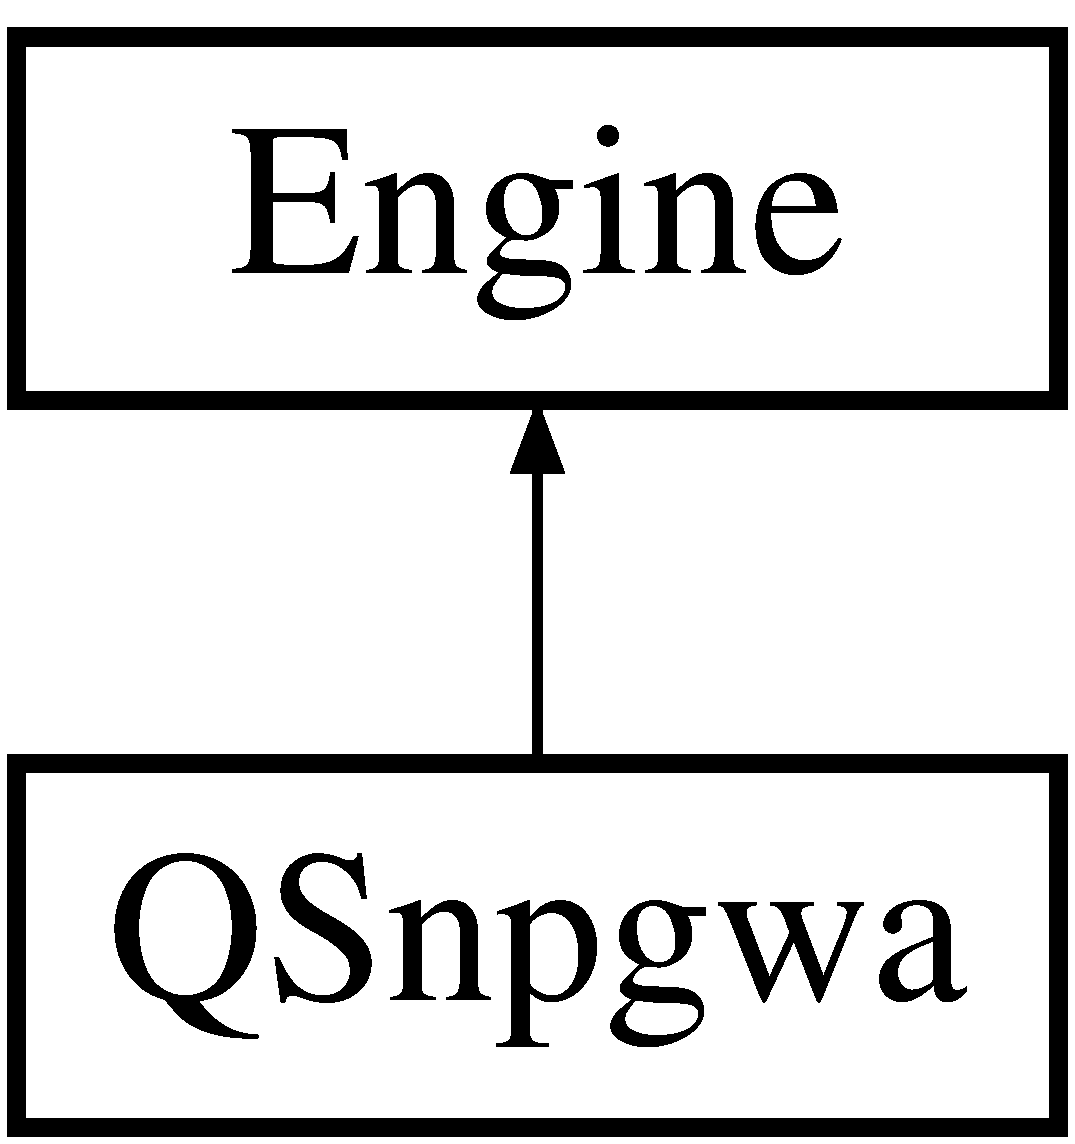
\includegraphics[height=2cm]{classQSnpgwa}
\end{center}
\end{figure}
\subsection*{Public Member Functions}
\begin{DoxyCompactItemize}
\item 
\hyperlink{classQSnpgwa_a348176fb642698c7756df9039b77109f}{QSnpgwa} ()
\item 
\hyperlink{classQSnpgwa_a762e315fb2455be5a553083af082b07d}{$\sim$QSnpgwa} ()
\item 
virtual void \hyperlink{classQSnpgwa_ac228fcbfcba981d48a223e911673e406}{init} ()
\item 
virtual void \hyperlink{classQSnpgwa_acc9e7d7e48d9c3e2fbb0a75e263f0c50}{preProcess} ()
\item 
virtual void \hyperlink{classQSnpgwa_a4873c7584d427c41a01e1bba159cf486}{process} ()
\item 
virtual void \hyperlink{classQSnpgwa_a2c39271b1001005e6d5a451dbc2fd8bb}{enslave} (\hyperlink{classEngineParamReader}{EngineParamReader} $\ast$)
\item 
virtual void \hyperlink{classQSnpgwa_aa127cdd0a042058f1ecab33d831a58a6}{test} ()
\end{DoxyCompactItemize}
\subsection*{Protected Member Functions}
\begin{DoxyCompactItemize}
\item 
void \hyperlink{classQSnpgwa_a30919016fc64635fcf65ca8771af504b}{delete\_\-my\_\-innards} ()
\item 
void \hyperlink{classQSnpgwa_a882fa04dd74b9772bbd452d5acc0dfb8}{initToZero} (\hyperlink{structContPopStatsResults}{ContPopStatsResults} \&p, \hyperlink{structContGenoStatsResults}{ContGenoStatsResults} \&ge)
\end{DoxyCompactItemize}
\subsection*{Protected Attributes}
\begin{DoxyCompactItemize}
\item 
\hyperlink{classEngineParamReader}{EngineParamReader} $\ast$ \hyperlink{classQSnpgwa_a357c8bf58fba34a5076eeb8f61a3cacb}{snp\_\-param}
\item 
\hyperlink{classQSnpgwaOutput}{QSnpgwaOutput} \hyperlink{classQSnpgwa_a0a854b526dee6f1552f280e63068e0a5}{out}
\item 
int \hyperlink{classQSnpgwa_a8134614250816926749e019ab6654344}{numInitSNPs}
\item 
int \hyperlink{classQSnpgwa_a04b7ca3253113ce5e2f5b9e1421161a1}{numInitPhen}
\item 
int \hyperlink{classQSnpgwa_ac7f80fcdcd53d7f8265bdd0591ea5fc9}{numFinalPhen}
\end{DoxyCompactItemize}


\subsection{Detailed Description}
Perform single locus tests using a quantitative phenotype and zero or more covariates.

\begin{DoxyAuthor}{Author}
Richard T. Guy 

Joshua Grab 

Matt Steigert 

Carl D. Langefeld 
\end{DoxyAuthor}


\subsection{Constructor \& Destructor Documentation}
\hypertarget{classQSnpgwa_a348176fb642698c7756df9039b77109f}{
\index{QSnpgwa@{QSnpgwa}!QSnpgwa@{QSnpgwa}}
\index{QSnpgwa@{QSnpgwa}!QSnpgwa@{QSnpgwa}}
\subsubsection[{QSnpgwa}]{\setlength{\rightskip}{0pt plus 5cm}QSnpgwa::QSnpgwa ()\hspace{0.3cm}{\ttfamily  \mbox{[}explicit\mbox{]}}}}
\label{classQSnpgwa_a348176fb642698c7756df9039b77109f}
\hypertarget{classQSnpgwa_a762e315fb2455be5a553083af082b07d}{
\index{QSnpgwa@{QSnpgwa}!$\sim$QSnpgwa@{$\sim$QSnpgwa}}
\index{$\sim$QSnpgwa@{$\sim$QSnpgwa}!QSnpgwa@{QSnpgwa}}
\subsubsection[{$\sim$QSnpgwa}]{\setlength{\rightskip}{0pt plus 5cm}QSnpgwa::$\sim$QSnpgwa ()}}
\label{classQSnpgwa_a762e315fb2455be5a553083af082b07d}


\subsection{Member Function Documentation}
\hypertarget{classQSnpgwa_a30919016fc64635fcf65ca8771af504b}{
\index{QSnpgwa@{QSnpgwa}!delete\_\-my\_\-innards@{delete\_\-my\_\-innards}}
\index{delete\_\-my\_\-innards@{delete\_\-my\_\-innards}!QSnpgwa@{QSnpgwa}}
\subsubsection[{delete\_\-my\_\-innards}]{\setlength{\rightskip}{0pt plus 5cm}void QSnpgwa::delete\_\-my\_\-innards ()\hspace{0.3cm}{\ttfamily  \mbox{[}protected\mbox{]}}}}
\label{classQSnpgwa_a30919016fc64635fcf65ca8771af504b}
\hypertarget{classQSnpgwa_a2c39271b1001005e6d5a451dbc2fd8bb}{
\index{QSnpgwa@{QSnpgwa}!enslave@{enslave}}
\index{enslave@{enslave}!QSnpgwa@{QSnpgwa}}
\subsubsection[{enslave}]{\setlength{\rightskip}{0pt plus 5cm}void QSnpgwa::enslave ({\bf EngineParamReader} $\ast$)\hspace{0.3cm}{\ttfamily  \mbox{[}virtual\mbox{]}}}}
\label{classQSnpgwa_a2c39271b1001005e6d5a451dbc2fd8bb}


Implements \hyperlink{classEngine_a023e094182312b1732fe53754c2fe5cb}{Engine}.

\hypertarget{classQSnpgwa_ac228fcbfcba981d48a223e911673e406}{
\index{QSnpgwa@{QSnpgwa}!init@{init}}
\index{init@{init}!QSnpgwa@{QSnpgwa}}
\subsubsection[{init}]{\setlength{\rightskip}{0pt plus 5cm}void QSnpgwa::init ()\hspace{0.3cm}{\ttfamily  \mbox{[}virtual\mbox{]}}}}
\label{classQSnpgwa_ac228fcbfcba981d48a223e911673e406}


Implements \hyperlink{classEngine_aaa054d596fb8ced6e3eb4bee208f8c3d}{Engine}.

\hypertarget{classQSnpgwa_a882fa04dd74b9772bbd452d5acc0dfb8}{
\index{QSnpgwa@{QSnpgwa}!initToZero@{initToZero}}
\index{initToZero@{initToZero}!QSnpgwa@{QSnpgwa}}
\subsubsection[{initToZero}]{\setlength{\rightskip}{0pt plus 5cm}void QSnpgwa::initToZero ({\bf ContPopStatsResults} \& {\em p}, \/  {\bf ContGenoStatsResults} \& {\em ge})\hspace{0.3cm}{\ttfamily  \mbox{[}protected\mbox{]}}}}
\label{classQSnpgwa_a882fa04dd74b9772bbd452d5acc0dfb8}
\hypertarget{classQSnpgwa_acc9e7d7e48d9c3e2fbb0a75e263f0c50}{
\index{QSnpgwa@{QSnpgwa}!preProcess@{preProcess}}
\index{preProcess@{preProcess}!QSnpgwa@{QSnpgwa}}
\subsubsection[{preProcess}]{\setlength{\rightskip}{0pt plus 5cm}void QSnpgwa::preProcess ()\hspace{0.3cm}{\ttfamily  \mbox{[}virtual\mbox{]}}}}
\label{classQSnpgwa_acc9e7d7e48d9c3e2fbb0a75e263f0c50}


Implements \hyperlink{classEngine_aec7076b8979a13c96eceb362437dc68c}{Engine}.

\hypertarget{classQSnpgwa_a4873c7584d427c41a01e1bba159cf486}{
\index{QSnpgwa@{QSnpgwa}!process@{process}}
\index{process@{process}!QSnpgwa@{QSnpgwa}}
\subsubsection[{process}]{\setlength{\rightskip}{0pt plus 5cm}void QSnpgwa::process ()\hspace{0.3cm}{\ttfamily  \mbox{[}virtual\mbox{]}}}}
\label{classQSnpgwa_a4873c7584d427c41a01e1bba159cf486}


Implements \hyperlink{classEngine_a005f8e277c3dea16ea05803fba223db7}{Engine}.

\hypertarget{classQSnpgwa_aa127cdd0a042058f1ecab33d831a58a6}{
\index{QSnpgwa@{QSnpgwa}!test@{test}}
\index{test@{test}!QSnpgwa@{QSnpgwa}}
\subsubsection[{test}]{\setlength{\rightskip}{0pt plus 5cm}void QSnpgwa::test ()\hspace{0.3cm}{\ttfamily  \mbox{[}virtual\mbox{]}}}}
\label{classQSnpgwa_aa127cdd0a042058f1ecab33d831a58a6}


Implements \hyperlink{classEngine_a2927c4a4263809453063ad482c6434a4}{Engine}.



\subsection{Field Documentation}
\hypertarget{classQSnpgwa_ac7f80fcdcd53d7f8265bdd0591ea5fc9}{
\index{QSnpgwa@{QSnpgwa}!numFinalPhen@{numFinalPhen}}
\index{numFinalPhen@{numFinalPhen}!QSnpgwa@{QSnpgwa}}
\subsubsection[{numFinalPhen}]{\setlength{\rightskip}{0pt plus 5cm}int {\bf QSnpgwa::numFinalPhen}\hspace{0.3cm}{\ttfamily  \mbox{[}protected\mbox{]}}}}
\label{classQSnpgwa_ac7f80fcdcd53d7f8265bdd0591ea5fc9}
\hypertarget{classQSnpgwa_a04b7ca3253113ce5e2f5b9e1421161a1}{
\index{QSnpgwa@{QSnpgwa}!numInitPhen@{numInitPhen}}
\index{numInitPhen@{numInitPhen}!QSnpgwa@{QSnpgwa}}
\subsubsection[{numInitPhen}]{\setlength{\rightskip}{0pt plus 5cm}int {\bf QSnpgwa::numInitPhen}\hspace{0.3cm}{\ttfamily  \mbox{[}protected\mbox{]}}}}
\label{classQSnpgwa_a04b7ca3253113ce5e2f5b9e1421161a1}
\hypertarget{classQSnpgwa_a8134614250816926749e019ab6654344}{
\index{QSnpgwa@{QSnpgwa}!numInitSNPs@{numInitSNPs}}
\index{numInitSNPs@{numInitSNPs}!QSnpgwa@{QSnpgwa}}
\subsubsection[{numInitSNPs}]{\setlength{\rightskip}{0pt plus 5cm}int {\bf QSnpgwa::numInitSNPs}\hspace{0.3cm}{\ttfamily  \mbox{[}protected\mbox{]}}}}
\label{classQSnpgwa_a8134614250816926749e019ab6654344}
\hypertarget{classQSnpgwa_a0a854b526dee6f1552f280e63068e0a5}{
\index{QSnpgwa@{QSnpgwa}!out@{out}}
\index{out@{out}!QSnpgwa@{QSnpgwa}}
\subsubsection[{out}]{\setlength{\rightskip}{0pt plus 5cm}{\bf QSnpgwaOutput} {\bf QSnpgwa::out}\hspace{0.3cm}{\ttfamily  \mbox{[}protected\mbox{]}}}}
\label{classQSnpgwa_a0a854b526dee6f1552f280e63068e0a5}
\hypertarget{classQSnpgwa_a357c8bf58fba34a5076eeb8f61a3cacb}{
\index{QSnpgwa@{QSnpgwa}!snp\_\-param@{snp\_\-param}}
\index{snp\_\-param@{snp\_\-param}!QSnpgwa@{QSnpgwa}}
\subsubsection[{snp\_\-param}]{\setlength{\rightskip}{0pt plus 5cm}{\bf EngineParamReader}$\ast$ {\bf QSnpgwa::snp\_\-param}\hspace{0.3cm}{\ttfamily  \mbox{[}protected\mbox{]}}}}
\label{classQSnpgwa_a357c8bf58fba34a5076eeb8f61a3cacb}


The documentation for this class was generated from the following files:\begin{DoxyCompactItemize}
\item 
engine/qsnpgwa/\hyperlink{qsnpgwa_8hh}{qsnpgwa.hh}\item 
engine/qsnpgwa/\hyperlink{qsnpgwa_8cpp}{qsnpgwa.cpp}\end{DoxyCompactItemize}

\hypertarget{classQSnpgwaException}{
\section{QSnpgwaException Class Reference}
\label{classQSnpgwaException}\index{QSnpgwaException@{QSnpgwaException}}
}


{\ttfamily \#include $<$exceptions.h$>$}

Inheritance diagram for QSnpgwaException:\begin{figure}[H]
\begin{center}
\leavevmode
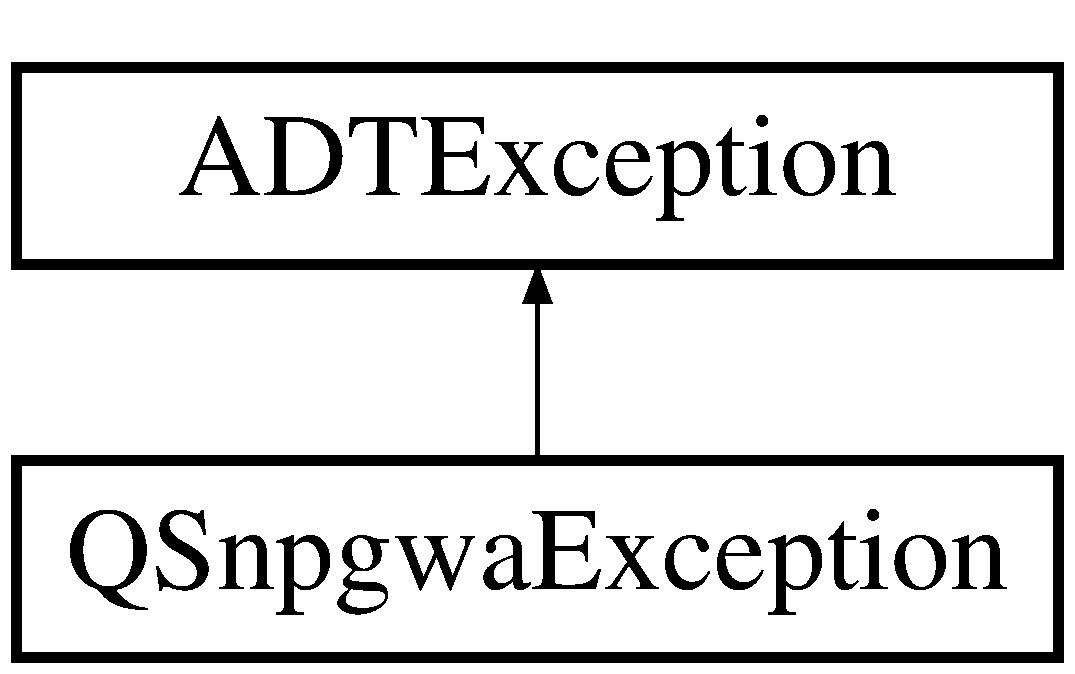
\includegraphics[height=2cm]{classQSnpgwaException}
\end{center}
\end{figure}


The documentation for this class was generated from the following file:\begin{DoxyCompactItemize}
\item 
engine/utils/\hyperlink{exceptions_8h}{exceptions.h}\end{DoxyCompactItemize}

\hypertarget{classQSnpgwaOutput}{
\section{QSnpgwaOutput Class Reference}
\label{classQSnpgwaOutput}\index{QSnpgwaOutput@{QSnpgwaOutput}}
}


{\ttfamily \#include $<$qsnpgwa\_\-out.hh$>$}

\subsection*{Public Member Functions}
\begin{DoxyCompactItemize}
\item 
\hyperlink{classQSnpgwaOutput_aa98c99a13210b4c8f90efe61afaf1725}{QSnpgwaOutput} ()
\item 
\hyperlink{classQSnpgwaOutput_a7c50b01f0631f1270add06dfb0abf8fc}{$\sim$QSnpgwaOutput} ()
\item 
bool \hyperlink{classQSnpgwaOutput_acea3297b5738eb71047385cd4c5ab1e8}{init} (\hyperlink{classParamReader}{ParamReader} $\ast$param, \hyperlink{classEngineParamReader}{EngineParamReader} $\ast$eparams, int maxMapSize, string message)
\item 
void \hyperlink{classQSnpgwaOutput_ab10d065c1d34ed8be33a423b6d30f297}{close} ()
\end{DoxyCompactItemize}
\subsection*{Protected Member Functions}
\begin{DoxyCompactItemize}
\item 
void \hyperlink{classQSnpgwaOutput_a336d56863a352e38d8a7e5ad1b340cae}{writeLine} (int idx, \hyperlink{classSnpInfo}{SnpInfo} \&q, const \hyperlink{structContPopStatsResults}{ContPopStatsResults} \&cp, const \hyperlink{structContGenoStatsResults}{ContGenoStatsResults} \&cg)
\item 
void \hyperlink{classQSnpgwaOutput_a9574fd93e422682b25033e41a9c3b72b}{writeHWELine} (int ids)
\item 
void \hyperlink{classQSnpgwaOutput_a5feff7620e8e5ba31ea11f2386f98538}{writeMainHeader} (\hyperlink{classOutput}{Output} \&, \hyperlink{classParamReader}{ParamReader} $\ast$)
\item 
void \hyperlink{classQSnpgwaOutput_a8dd9ee1d5afed7e6eb72d1aa525081eb}{writeMainLegend} (\hyperlink{classOutput}{Output} \&)
\item 
void \hyperlink{classQSnpgwaOutput_a2b0ca6d197ec6b9155bc051e29627665}{writeHWELegend} (\hyperlink{classOutput}{Output} \&)
\item 
void \hyperlink{classQSnpgwaOutput_abeeb5f390c652631a711d1aa1f847d87}{writeHWELine} (int idx, const \hyperlink{classSnpInfo}{SnpInfo} \&s, const \hyperlink{structContPopStatsResults}{ContPopStatsResults} \&p)
\end{DoxyCompactItemize}
\subsection*{Protected Attributes}
\begin{DoxyCompactItemize}
\item 
\hyperlink{classOutput}{Output} \hyperlink{classQSnpgwaOutput_ac3038412ce272d15749e62d487d1bf76}{outMain}
\item 
\hyperlink{classOutput}{Output} \hyperlink{classQSnpgwaOutput_a13210554d75274ea4e2fd14480e6144b}{outGeno1}
\item 
\hyperlink{classOutput}{Output} \hyperlink{classQSnpgwaOutput_a94e142191f1b20e3ea9ed7d5619d6537}{outGeno2}
\item 
\hyperlink{classOutput}{Output} \hyperlink{classQSnpgwaOutput_add4f3d1c02269a63a8ca9ab6b6a6692b}{outGeno3}
\item 
\hyperlink{classOutput}{Output} \hyperlink{classQSnpgwaOutput_ae8e2c64a3863e19f6a20835f77c74888}{outHWE}
\item 
\hyperlink{classOutput}{Output} \hyperlink{classQSnpgwaOutput_a9a500d66e2a2f4e0a2f2a361cf4769a4}{outRefAllele}
\item 
bool \hyperlink{classQSnpgwaOutput_a623e09a643beb7b19ffe68037571bb2f}{writeGenoFiles}
\item 
bool \hyperlink{classQSnpgwaOutput_aa3fe3500366b73d73c6ede530c2962c3}{writeHWEFiles}
\item 
bool \hyperlink{classQSnpgwaOutput_a17d5eb6f91e4e3c88c8215c194a47130}{writeRefFile}
\item 
bool \hyperlink{classQSnpgwaOutput_a4962e53bdd5892a0737e5f91c6cb1099}{writeMainFileMap}
\item 
bool \hyperlink{classQSnpgwaOutput_a289ac8eef9d3d51610541bfbec316c7c}{writeMainFileHap}
\item 
int \hyperlink{classQSnpgwaOutput_afd9b23c1ded591a794688c9ebb58103b}{mapSize}
\end{DoxyCompactItemize}
\subsection*{Friends}
\begin{DoxyCompactItemize}
\item 
class \hyperlink{classQSnpgwaOutput_a7db91fc2b62ffb71edee988fd8f7f575}{QSnpgwa}
\end{DoxyCompactItemize}


\subsection{Constructor \& Destructor Documentation}
\hypertarget{classQSnpgwaOutput_aa98c99a13210b4c8f90efe61afaf1725}{
\index{QSnpgwaOutput@{QSnpgwaOutput}!QSnpgwaOutput@{QSnpgwaOutput}}
\index{QSnpgwaOutput@{QSnpgwaOutput}!QSnpgwaOutput@{QSnpgwaOutput}}
\subsubsection[{QSnpgwaOutput}]{\setlength{\rightskip}{0pt plus 5cm}QSnpgwaOutput::QSnpgwaOutput ()}}
\label{classQSnpgwaOutput_aa98c99a13210b4c8f90efe61afaf1725}
\hypertarget{classQSnpgwaOutput_a7c50b01f0631f1270add06dfb0abf8fc}{
\index{QSnpgwaOutput@{QSnpgwaOutput}!$\sim$QSnpgwaOutput@{$\sim$QSnpgwaOutput}}
\index{$\sim$QSnpgwaOutput@{$\sim$QSnpgwaOutput}!QSnpgwaOutput@{QSnpgwaOutput}}
\subsubsection[{$\sim$QSnpgwaOutput}]{\setlength{\rightskip}{0pt plus 5cm}QSnpgwaOutput::$\sim$QSnpgwaOutput ()}}
\label{classQSnpgwaOutput_a7c50b01f0631f1270add06dfb0abf8fc}


\subsection{Member Function Documentation}
\hypertarget{classQSnpgwaOutput_ab10d065c1d34ed8be33a423b6d30f297}{
\index{QSnpgwaOutput@{QSnpgwaOutput}!close@{close}}
\index{close@{close}!QSnpgwaOutput@{QSnpgwaOutput}}
\subsubsection[{close}]{\setlength{\rightskip}{0pt plus 5cm}void QSnpgwaOutput::close ()}}
\label{classQSnpgwaOutput_ab10d065c1d34ed8be33a423b6d30f297}
\hypertarget{classQSnpgwaOutput_acea3297b5738eb71047385cd4c5ab1e8}{
\index{QSnpgwaOutput@{QSnpgwaOutput}!init@{init}}
\index{init@{init}!QSnpgwaOutput@{QSnpgwaOutput}}
\subsubsection[{init}]{\setlength{\rightskip}{0pt plus 5cm}bool QSnpgwaOutput::init ({\bf ParamReader} $\ast$ {\em param}, \/  {\bf EngineParamReader} $\ast$ {\em eparams}, \/  int {\em maxMapSize}, \/  string {\em message})}}
\label{classQSnpgwaOutput_acea3297b5738eb71047385cd4c5ab1e8}
\hypertarget{classQSnpgwaOutput_a2b0ca6d197ec6b9155bc051e29627665}{
\index{QSnpgwaOutput@{QSnpgwaOutput}!writeHWELegend@{writeHWELegend}}
\index{writeHWELegend@{writeHWELegend}!QSnpgwaOutput@{QSnpgwaOutput}}
\subsubsection[{writeHWELegend}]{\setlength{\rightskip}{0pt plus 5cm}void QSnpgwaOutput::writeHWELegend ({\bf Output} \& {\em out})\hspace{0.3cm}{\ttfamily  \mbox{[}protected\mbox{]}}}}
\label{classQSnpgwaOutput_a2b0ca6d197ec6b9155bc051e29627665}
Write legend for HWE \hypertarget{classQSnpgwaOutput_abeeb5f390c652631a711d1aa1f847d87}{
\index{QSnpgwaOutput@{QSnpgwaOutput}!writeHWELine@{writeHWELine}}
\index{writeHWELine@{writeHWELine}!QSnpgwaOutput@{QSnpgwaOutput}}
\subsubsection[{writeHWELine}]{\setlength{\rightskip}{0pt plus 5cm}void QSnpgwaOutput::writeHWELine (int {\em idx}, \/  const {\bf SnpInfo} \& {\em s}, \/  const {\bf ContPopStatsResults} \& {\em p})\hspace{0.3cm}{\ttfamily  \mbox{[}protected\mbox{]}}}}
\label{classQSnpgwaOutput_abeeb5f390c652631a711d1aa1f847d87}
\hypertarget{classQSnpgwaOutput_a9574fd93e422682b25033e41a9c3b72b}{
\index{QSnpgwaOutput@{QSnpgwaOutput}!writeHWELine@{writeHWELine}}
\index{writeHWELine@{writeHWELine}!QSnpgwaOutput@{QSnpgwaOutput}}
\subsubsection[{writeHWELine}]{\setlength{\rightskip}{0pt plus 5cm}void QSnpgwaOutput::writeHWELine (int {\em ids})\hspace{0.3cm}{\ttfamily  \mbox{[}protected\mbox{]}}}}
\label{classQSnpgwaOutput_a9574fd93e422682b25033e41a9c3b72b}
\hypertarget{classQSnpgwaOutput_a336d56863a352e38d8a7e5ad1b340cae}{
\index{QSnpgwaOutput@{QSnpgwaOutput}!writeLine@{writeLine}}
\index{writeLine@{writeLine}!QSnpgwaOutput@{QSnpgwaOutput}}
\subsubsection[{writeLine}]{\setlength{\rightskip}{0pt plus 5cm}void QSnpgwaOutput::writeLine (int {\em idx}, \/  {\bf SnpInfo} \& {\em q}, \/  const {\bf ContPopStatsResults} \& {\em cp}, \/  const {\bf ContGenoStatsResults} \& {\em cg})\hspace{0.3cm}{\ttfamily  \mbox{[}protected\mbox{]}}}}
\label{classQSnpgwaOutput_a336d56863a352e38d8a7e5ad1b340cae}
Write a line. \hypertarget{classQSnpgwaOutput_a5feff7620e8e5ba31ea11f2386f98538}{
\index{QSnpgwaOutput@{QSnpgwaOutput}!writeMainHeader@{writeMainHeader}}
\index{writeMainHeader@{writeMainHeader}!QSnpgwaOutput@{QSnpgwaOutput}}
\subsubsection[{writeMainHeader}]{\setlength{\rightskip}{0pt plus 5cm}void QSnpgwaOutput::writeMainHeader ({\bf Output} \& {\em out}, \/  {\bf ParamReader} $\ast$ {\em param})\hspace{0.3cm}{\ttfamily  \mbox{[}protected\mbox{]}}}}
\label{classQSnpgwaOutput_a5feff7620e8e5ba31ea11f2386f98538}
Write the header for the main output. \hypertarget{classQSnpgwaOutput_a8dd9ee1d5afed7e6eb72d1aa525081eb}{
\index{QSnpgwaOutput@{QSnpgwaOutput}!writeMainLegend@{writeMainLegend}}
\index{writeMainLegend@{writeMainLegend}!QSnpgwaOutput@{QSnpgwaOutput}}
\subsubsection[{writeMainLegend}]{\setlength{\rightskip}{0pt plus 5cm}void QSnpgwaOutput::writeMainLegend ({\bf Output} \& {\em out})\hspace{0.3cm}{\ttfamily  \mbox{[}protected\mbox{]}}}}
\label{classQSnpgwaOutput_a8dd9ee1d5afed7e6eb72d1aa525081eb}
Write the main output legend. 

\subsection{Friends And Related Function Documentation}
\hypertarget{classQSnpgwaOutput_a7db91fc2b62ffb71edee988fd8f7f575}{
\index{QSnpgwaOutput@{QSnpgwaOutput}!QSnpgwa@{QSnpgwa}}
\index{QSnpgwa@{QSnpgwa}!QSnpgwaOutput@{QSnpgwaOutput}}
\subsubsection[{QSnpgwa}]{\setlength{\rightskip}{0pt plus 5cm}friend class {\bf QSnpgwa}\hspace{0.3cm}{\ttfamily  \mbox{[}friend\mbox{]}}}}
\label{classQSnpgwaOutput_a7db91fc2b62ffb71edee988fd8f7f575}


\subsection{Field Documentation}
\hypertarget{classQSnpgwaOutput_afd9b23c1ded591a794688c9ebb58103b}{
\index{QSnpgwaOutput@{QSnpgwaOutput}!mapSize@{mapSize}}
\index{mapSize@{mapSize}!QSnpgwaOutput@{QSnpgwaOutput}}
\subsubsection[{mapSize}]{\setlength{\rightskip}{0pt plus 5cm}int {\bf QSnpgwaOutput::mapSize}\hspace{0.3cm}{\ttfamily  \mbox{[}protected\mbox{]}}}}
\label{classQSnpgwaOutput_afd9b23c1ded591a794688c9ebb58103b}
\hypertarget{classQSnpgwaOutput_a13210554d75274ea4e2fd14480e6144b}{
\index{QSnpgwaOutput@{QSnpgwaOutput}!outGeno1@{outGeno1}}
\index{outGeno1@{outGeno1}!QSnpgwaOutput@{QSnpgwaOutput}}
\subsubsection[{outGeno1}]{\setlength{\rightskip}{0pt plus 5cm}{\bf Output} {\bf QSnpgwaOutput::outGeno1}\hspace{0.3cm}{\ttfamily  \mbox{[}protected\mbox{]}}}}
\label{classQSnpgwaOutput_a13210554d75274ea4e2fd14480e6144b}
\hypertarget{classQSnpgwaOutput_a94e142191f1b20e3ea9ed7d5619d6537}{
\index{QSnpgwaOutput@{QSnpgwaOutput}!outGeno2@{outGeno2}}
\index{outGeno2@{outGeno2}!QSnpgwaOutput@{QSnpgwaOutput}}
\subsubsection[{outGeno2}]{\setlength{\rightskip}{0pt plus 5cm}{\bf Output} {\bf QSnpgwaOutput::outGeno2}\hspace{0.3cm}{\ttfamily  \mbox{[}protected\mbox{]}}}}
\label{classQSnpgwaOutput_a94e142191f1b20e3ea9ed7d5619d6537}
\hypertarget{classQSnpgwaOutput_add4f3d1c02269a63a8ca9ab6b6a6692b}{
\index{QSnpgwaOutput@{QSnpgwaOutput}!outGeno3@{outGeno3}}
\index{outGeno3@{outGeno3}!QSnpgwaOutput@{QSnpgwaOutput}}
\subsubsection[{outGeno3}]{\setlength{\rightskip}{0pt plus 5cm}{\bf Output} {\bf QSnpgwaOutput::outGeno3}\hspace{0.3cm}{\ttfamily  \mbox{[}protected\mbox{]}}}}
\label{classQSnpgwaOutput_add4f3d1c02269a63a8ca9ab6b6a6692b}
\hypertarget{classQSnpgwaOutput_ae8e2c64a3863e19f6a20835f77c74888}{
\index{QSnpgwaOutput@{QSnpgwaOutput}!outHWE@{outHWE}}
\index{outHWE@{outHWE}!QSnpgwaOutput@{QSnpgwaOutput}}
\subsubsection[{outHWE}]{\setlength{\rightskip}{0pt plus 5cm}{\bf Output} {\bf QSnpgwaOutput::outHWE}\hspace{0.3cm}{\ttfamily  \mbox{[}protected\mbox{]}}}}
\label{classQSnpgwaOutput_ae8e2c64a3863e19f6a20835f77c74888}
\hypertarget{classQSnpgwaOutput_ac3038412ce272d15749e62d487d1bf76}{
\index{QSnpgwaOutput@{QSnpgwaOutput}!outMain@{outMain}}
\index{outMain@{outMain}!QSnpgwaOutput@{QSnpgwaOutput}}
\subsubsection[{outMain}]{\setlength{\rightskip}{0pt plus 5cm}{\bf Output} {\bf QSnpgwaOutput::outMain}\hspace{0.3cm}{\ttfamily  \mbox{[}protected\mbox{]}}}}
\label{classQSnpgwaOutput_ac3038412ce272d15749e62d487d1bf76}
\hypertarget{classQSnpgwaOutput_a9a500d66e2a2f4e0a2f2a361cf4769a4}{
\index{QSnpgwaOutput@{QSnpgwaOutput}!outRefAllele@{outRefAllele}}
\index{outRefAllele@{outRefAllele}!QSnpgwaOutput@{QSnpgwaOutput}}
\subsubsection[{outRefAllele}]{\setlength{\rightskip}{0pt plus 5cm}{\bf Output} {\bf QSnpgwaOutput::outRefAllele}\hspace{0.3cm}{\ttfamily  \mbox{[}protected\mbox{]}}}}
\label{classQSnpgwaOutput_a9a500d66e2a2f4e0a2f2a361cf4769a4}
\hypertarget{classQSnpgwaOutput_a623e09a643beb7b19ffe68037571bb2f}{
\index{QSnpgwaOutput@{QSnpgwaOutput}!writeGenoFiles@{writeGenoFiles}}
\index{writeGenoFiles@{writeGenoFiles}!QSnpgwaOutput@{QSnpgwaOutput}}
\subsubsection[{writeGenoFiles}]{\setlength{\rightskip}{0pt plus 5cm}bool {\bf QSnpgwaOutput::writeGenoFiles}\hspace{0.3cm}{\ttfamily  \mbox{[}protected\mbox{]}}}}
\label{classQSnpgwaOutput_a623e09a643beb7b19ffe68037571bb2f}
\hypertarget{classQSnpgwaOutput_aa3fe3500366b73d73c6ede530c2962c3}{
\index{QSnpgwaOutput@{QSnpgwaOutput}!writeHWEFiles@{writeHWEFiles}}
\index{writeHWEFiles@{writeHWEFiles}!QSnpgwaOutput@{QSnpgwaOutput}}
\subsubsection[{writeHWEFiles}]{\setlength{\rightskip}{0pt plus 5cm}bool {\bf QSnpgwaOutput::writeHWEFiles}\hspace{0.3cm}{\ttfamily  \mbox{[}protected\mbox{]}}}}
\label{classQSnpgwaOutput_aa3fe3500366b73d73c6ede530c2962c3}
\hypertarget{classQSnpgwaOutput_a289ac8eef9d3d51610541bfbec316c7c}{
\index{QSnpgwaOutput@{QSnpgwaOutput}!writeMainFileHap@{writeMainFileHap}}
\index{writeMainFileHap@{writeMainFileHap}!QSnpgwaOutput@{QSnpgwaOutput}}
\subsubsection[{writeMainFileHap}]{\setlength{\rightskip}{0pt plus 5cm}bool {\bf QSnpgwaOutput::writeMainFileHap}\hspace{0.3cm}{\ttfamily  \mbox{[}protected\mbox{]}}}}
\label{classQSnpgwaOutput_a289ac8eef9d3d51610541bfbec316c7c}
\hypertarget{classQSnpgwaOutput_a4962e53bdd5892a0737e5f91c6cb1099}{
\index{QSnpgwaOutput@{QSnpgwaOutput}!writeMainFileMap@{writeMainFileMap}}
\index{writeMainFileMap@{writeMainFileMap}!QSnpgwaOutput@{QSnpgwaOutput}}
\subsubsection[{writeMainFileMap}]{\setlength{\rightskip}{0pt plus 5cm}bool {\bf QSnpgwaOutput::writeMainFileMap}\hspace{0.3cm}{\ttfamily  \mbox{[}protected\mbox{]}}}}
\label{classQSnpgwaOutput_a4962e53bdd5892a0737e5f91c6cb1099}
\hypertarget{classQSnpgwaOutput_a17d5eb6f91e4e3c88c8215c194a47130}{
\index{QSnpgwaOutput@{QSnpgwaOutput}!writeRefFile@{writeRefFile}}
\index{writeRefFile@{writeRefFile}!QSnpgwaOutput@{QSnpgwaOutput}}
\subsubsection[{writeRefFile}]{\setlength{\rightskip}{0pt plus 5cm}bool {\bf QSnpgwaOutput::writeRefFile}\hspace{0.3cm}{\ttfamily  \mbox{[}protected\mbox{]}}}}
\label{classQSnpgwaOutput_a17d5eb6f91e4e3c88c8215c194a47130}


The documentation for this class was generated from the following files:\begin{DoxyCompactItemize}
\item 
engine/output/\hyperlink{qsnpgwa__out_8hh}{qsnpgwa\_\-out.hh}\item 
engine/output/\hyperlink{qsnpgwa__out_8cpp}{qsnpgwa\_\-out.cpp}\end{DoxyCompactItemize}

\hypertarget{classRandWH}{
\section{RandWH Class Reference}
\label{classRandWH}\index{RandWH@{RandWH}}
}


{\ttfamily \#include $<$randwh.h$>$}

\subsection*{Public Member Functions}
\begin{DoxyCompactItemize}
\item 
\hyperlink{classRandWH_ae9f57a6a9673f324f2403a51f03a9280}{RandWH} ()
\item 
void \hyperlink{classRandWH_a8c373ceb6c13088ae8053b9c5f79ccea}{init} (long seeds\mbox{[}$\,$\mbox{]})
\item 
void \hyperlink{classRandWH_ae18fe372528b36f76ed3c36ed4e8ebbf}{init} (char $\ast$)
\item 
void \hyperlink{classRandWH_a98737ce014ca577b4ab6af733a8056f9}{state} (char $\ast$)
\item 
double \hyperlink{classRandWH_aee09f663e825d7cd6f66eb8bd0200112}{get} ()
\item 
void \hyperlink{classRandWH_a3daac6243983e16e361f763ac0748777}{state} (long $\ast$s)
\end{DoxyCompactItemize}


\subsection{Constructor \& Destructor Documentation}
\hypertarget{classRandWH_ae9f57a6a9673f324f2403a51f03a9280}{
\index{RandWH@{RandWH}!RandWH@{RandWH}}
\index{RandWH@{RandWH}!RandWH@{RandWH}}
\subsubsection[{RandWH}]{\setlength{\rightskip}{0pt plus 5cm}RandWH::RandWH ()}}
\label{classRandWH_ae9f57a6a9673f324f2403a51f03a9280}


\subsection{Member Function Documentation}
\hypertarget{classRandWH_aee09f663e825d7cd6f66eb8bd0200112}{
\index{RandWH@{RandWH}!get@{get}}
\index{get@{get}!RandWH@{RandWH}}
\subsubsection[{get}]{\setlength{\rightskip}{0pt plus 5cm}double RandWH::get ()}}
\label{classRandWH_aee09f663e825d7cd6f66eb8bd0200112}
\hypertarget{classRandWH_ae18fe372528b36f76ed3c36ed4e8ebbf}{
\index{RandWH@{RandWH}!init@{init}}
\index{init@{init}!RandWH@{RandWH}}
\subsubsection[{init}]{\setlength{\rightskip}{0pt plus 5cm}void RandWH::init (char $\ast$ {\em filename})}}
\label{classRandWH_ae18fe372528b36f76ed3c36ed4e8ebbf}
\hypertarget{classRandWH_a8c373ceb6c13088ae8053b9c5f79ccea}{
\index{RandWH@{RandWH}!init@{init}}
\index{init@{init}!RandWH@{RandWH}}
\subsubsection[{init}]{\setlength{\rightskip}{0pt plus 5cm}void RandWH::init (long {\em seeds}\mbox{[}$\,$\mbox{]})}}
\label{classRandWH_a8c373ceb6c13088ae8053b9c5f79ccea}
\hypertarget{classRandWH_a3daac6243983e16e361f763ac0748777}{
\index{RandWH@{RandWH}!state@{state}}
\index{state@{state}!RandWH@{RandWH}}
\subsubsection[{state}]{\setlength{\rightskip}{0pt plus 5cm}void RandWH::state (long $\ast$ {\em s})}}
\label{classRandWH_a3daac6243983e16e361f763ac0748777}
\hypertarget{classRandWH_a98737ce014ca577b4ab6af733a8056f9}{
\index{RandWH@{RandWH}!state@{state}}
\index{state@{state}!RandWH@{RandWH}}
\subsubsection[{state}]{\setlength{\rightskip}{0pt plus 5cm}void RandWH::state (char $\ast$ {\em filename})}}
\label{classRandWH_a98737ce014ca577b4ab6af733a8056f9}


The documentation for this class was generated from the following files:\begin{DoxyCompactItemize}
\item 
engine/\hyperlink{randwh_8h}{randwh.h}\item 
engine/\hyperlink{randwh_8cpp}{randwh.cpp}\end{DoxyCompactItemize}

\hypertarget{classReader}{
\section{Reader Class Reference}
\label{classReader}\index{Reader@{Reader}}
}


{\ttfamily \#include $<$reader.h$>$}

Inheritance diagram for Reader:\begin{figure}[H]
\begin{center}
\leavevmode
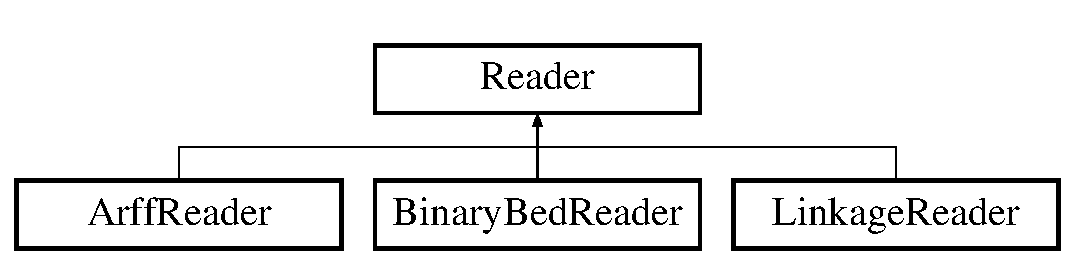
\includegraphics[height=2cm]{classReader}
\end{center}
\end{figure}
\subsection*{Public Member Functions}
\begin{DoxyCompactItemize}
\item 
virtual \hyperlink{classReader_a78089542fd27a0ac2df6702fffe8725c}{$\sim$Reader} ()
\item 
virtual void \hyperlink{classReader_a334a724f607c84262af67759ffcdbd26}{process} (\hyperlink{classSnpData}{SnpData} $\ast$, \hyperlink{classParamReader}{ParamReader} $\ast$)=0
\item 
bool \hyperlink{classReader_af1812be4a38c094fd2a34a13b784e554}{getLine} (ifstream $\ast$, vector$<$ string $>$ $\ast$, \hyperlink{classParamReader}{ParamReader} $\ast$, bool check)
\end{DoxyCompactItemize}


\subsection{Constructor \& Destructor Documentation}
\hypertarget{classReader_a78089542fd27a0ac2df6702fffe8725c}{
\index{Reader@{Reader}!$\sim$Reader@{$\sim$Reader}}
\index{$\sim$Reader@{$\sim$Reader}!Reader@{Reader}}
\subsubsection[{$\sim$Reader}]{\setlength{\rightskip}{0pt plus 5cm}Reader::$\sim$Reader ()\hspace{0.3cm}{\ttfamily  \mbox{[}virtual\mbox{]}}}}
\label{classReader_a78089542fd27a0ac2df6702fffe8725c}


\subsection{Member Function Documentation}
\hypertarget{classReader_af1812be4a38c094fd2a34a13b784e554}{
\index{Reader@{Reader}!getLine@{getLine}}
\index{getLine@{getLine}!Reader@{Reader}}
\subsubsection[{getLine}]{\setlength{\rightskip}{0pt plus 5cm}bool Reader::getLine (ifstream $\ast$ {\em infile}, \/  vector$<$ string $>$ $\ast$ {\em line}, \/  {\bf ParamReader} $\ast$ {\em params}, \/  bool {\em check\_\-used})}}
\label{classReader_af1812be4a38c094fd2a34a13b784e554}
\hyperlink{classReader_af1812be4a38c094fd2a34a13b784e554}{getLine()}

Returns a single line of arbitrary length from the file, splitting on spaces to create an array.

Clears the array before starting.


\begin{DoxyParams}{Parameters}
\item[{\em infile}]An incoming file stream \item[{\em line}]The address of the vector that should hold the tokenized line. \item[{\em params}]A parameter object \item[{\em check\_\-used}]Query this location agains the parameter object's use/not use information \end{DoxyParams}
\begin{DoxyReturn}{Returns}
Result of file-\/$>$eof() 
\end{DoxyReturn}
\hypertarget{classReader_a334a724f607c84262af67759ffcdbd26}{
\index{Reader@{Reader}!process@{process}}
\index{process@{process}!Reader@{Reader}}
\subsubsection[{process}]{\setlength{\rightskip}{0pt plus 5cm}virtual void Reader::process ({\bf SnpData} $\ast$, \/  {\bf ParamReader} $\ast$)\hspace{0.3cm}{\ttfamily  \mbox{[}pure virtual\mbox{]}}}}
\label{classReader_a334a724f607c84262af67759ffcdbd26}


Implemented in \hyperlink{classArffReader_af12ed42f6e726a6e336f22381ca84082}{ArffReader}, \hyperlink{classBinaryBedReader_a2132af8b71a683550c19ec4ac3ec3db2}{BinaryBedReader}, and \hyperlink{classLinkageReader_a808d3be4b0a2b3af8a7ec7fea963960b}{LinkageReader}.



The documentation for this class was generated from the following files:\begin{DoxyCompactItemize}
\item 
reader/\hyperlink{reader_8h}{reader.h}\item 
reader/\hyperlink{reader_8cpp}{reader.cpp}\end{DoxyCompactItemize}

\hypertarget{classRunOrderException}{
\section{RunOrderException Class Reference}
\label{classRunOrderException}\index{RunOrderException@{RunOrderException}}
}


{\ttfamily \#include $<$exceptions.h$>$}

Inheritance diagram for RunOrderException:\begin{figure}[H]
\begin{center}
\leavevmode
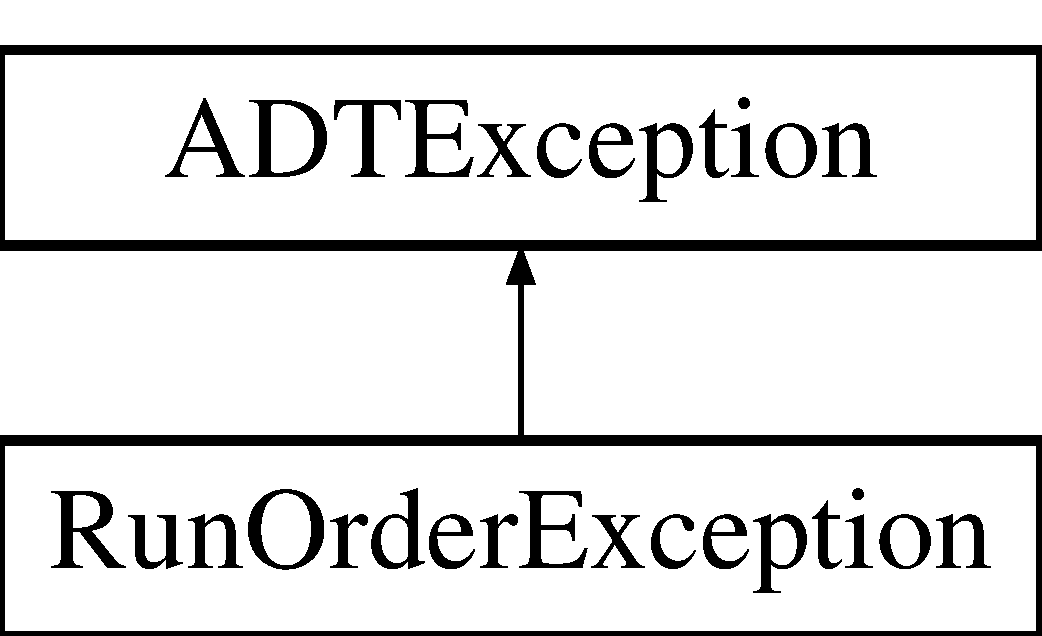
\includegraphics[height=2cm]{classRunOrderException}
\end{center}
\end{figure}
\subsection*{Data Fields}
\begin{DoxyCompactItemize}
\item 
string \hyperlink{classRunOrderException_aed5972b7666d8edb24f9ffe4ef4ed4d2}{message}
\end{DoxyCompactItemize}


\subsection{Detailed Description}
Used when something called out of order. 

\subsection{Field Documentation}
\hypertarget{classRunOrderException_aed5972b7666d8edb24f9ffe4ef4ed4d2}{
\index{RunOrderException@{RunOrderException}!message@{message}}
\index{message@{message}!RunOrderException@{RunOrderException}}
\subsubsection[{message}]{\setlength{\rightskip}{0pt plus 5cm}string {\bf RunOrderException::message}}}
\label{classRunOrderException_aed5972b7666d8edb24f9ffe4ef4ed4d2}


The documentation for this class was generated from the following file:\begin{DoxyCompactItemize}
\item 
engine/utils/\hyperlink{exceptions_8h}{exceptions.h}\end{DoxyCompactItemize}

\hypertarget{classSingularMatrixEx}{
\section{SingularMatrixEx Class Reference}
\label{classSingularMatrixEx}\index{SingularMatrixEx@{SingularMatrixEx}}
}


{\ttfamily \#include $<$exceptions.h$>$}

Inheritance diagram for SingularMatrixEx:\begin{figure}[H]
\begin{center}
\leavevmode
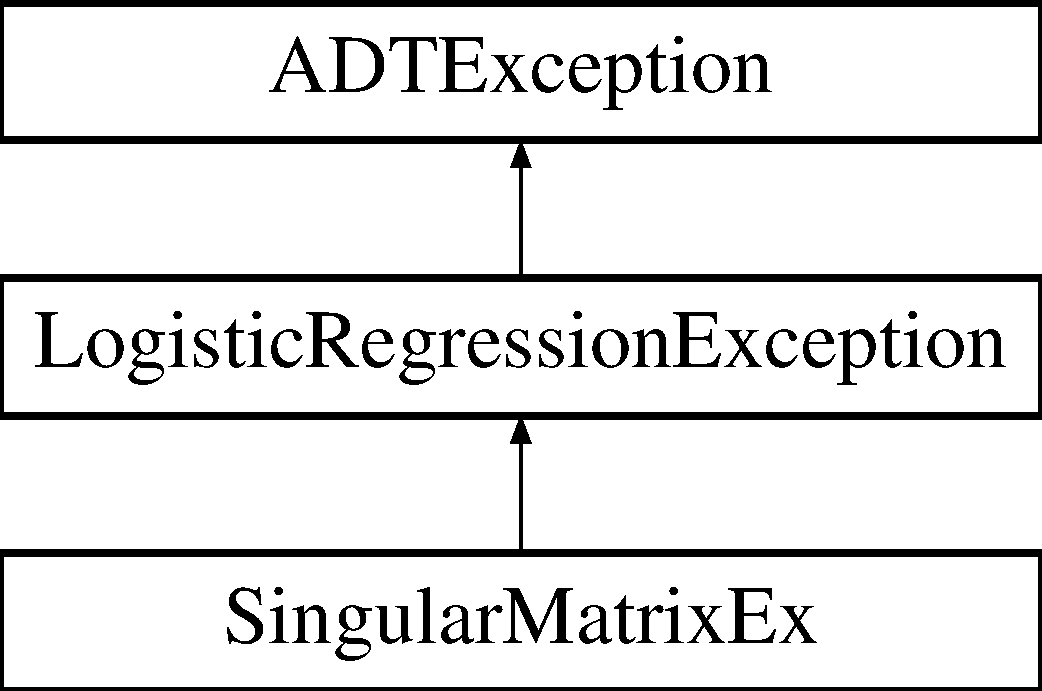
\includegraphics[height=3cm]{classSingularMatrixEx}
\end{center}
\end{figure}


The documentation for this class was generated from the following file:\begin{DoxyCompactItemize}
\item 
engine/utils/\hyperlink{exceptions_8h}{exceptions.h}\end{DoxyCompactItemize}

\hypertarget{classSnpData}{
\section{SnpData Class Reference}
\label{classSnpData}\index{SnpData@{SnpData}}
}


{\ttfamily \#include $<$snp\_\-data.hh$>$}

\subsection*{Data Structures}
\begin{DoxyCompactItemize}
\item 
struct \hyperlink{structSnpData_1_1MapData}{MapData}
\end{DoxyCompactItemize}
\subsection*{Public Member Functions}
\begin{DoxyCompactItemize}
\item 
\hyperlink{classSnpData_a67ecd2aa4fd9d991117724c025d4fe8b}{SnpData} ()
\item 
\hyperlink{classSnpData_ae8f5c2288be6040daaeacf2a00a6cc5e}{$\sim$SnpData} ()
\item 
void \hyperlink{classSnpData_afde9baf5271d4ccd8a47bba6a7a3a25c}{push\_\-map} (string, string, long, char ref=(char) 0)
\item 
void \hyperlink{classSnpData_a7154ea651a58dc4d2fa5398acfa85780}{setIndividualName} (unsigned int i, string name)
\item 
void \hyperlink{classSnpData_ae6d6c89606d8176f34b11b253b40f191}{cleanIndividualNames} ()
\item 
void \hyperlink{classSnpData_a856afb537dc90f0e45c2d3a28d6a8b41}{prep\_\-data} (\hyperlink{classParamReader}{ParamReader} $\ast$)
\begin{DoxyCompactList}\small\item\em Data cleaning functions. \item\end{DoxyCompactList}\item 
void \hyperlink{classSnpData_a5f986138c94a1a0491bd56f5d0b9eb14}{categorical\_\-phenotype} (int low, int hi)
\item 
void \hyperlink{classSnpData_a6c174381b8ca1a605e7e052990b563ce}{remove\_\-haplotype} ()
\item 
int \hyperlink{classSnpData_a0056036c39385fa3e2955162755be872}{remove\_\-phenotype} (double)
\item 
int \hyperlink{classSnpData_a9fa11c7060c6eba27c09c38c8366d8d1}{remove\_\-covariate} (double)
\item 
int \hyperlink{classSnpData_ac7952b0c911c5c3f7a894ab3c5b9c179}{remove\_\-indiv\_\-with\_\-snp\_\-value} (int)
\item 
int \hyperlink{classSnpData_afadaf2a77dc7b57c53c35bfda981bbc8}{remove\_\-missing\_\-geno} ()
\item 
bool \hyperlink{classSnpData_adcde7db42d75082f1ff23379c0a52caa}{isUsable} (int i)
\item 
bool \hyperlink{classSnpData_a4aed56566f1194ab787b604563783280}{delete\_\-snp} (long l)
\begin{DoxyCompactList}\small\item\em Data manipulation functions. \item\end{DoxyCompactList}\item 
void \hyperlink{classSnpData_afc11539758009ab2d5cd4f2b04f7c1bd}{snp\_\-flush} ()
\item 
bool \hyperlink{classSnpData_af7caa689a8257f534cd6a92dac45ee82}{delete\_\-indiv} (int i)
\item 
void \hyperlink{classSnpData_ad2089f56539d02ab64282473b0ca9bd0}{indiv\_\-flush} ()
\item 
void \hyperlink{classSnpData_a55e5ee9b74b0b6057393d8e19dd8fced}{dump\_\-data} ()
\end{DoxyCompactItemize}
\subsection*{Data Fields}
\begin{DoxyCompactItemize}
\item 
vector$<$ char $>$ \hyperlink{classSnpData_a3e88fcb82912de7cb1e37e2630bbee71}{character\_\-list}
\end{DoxyCompactItemize}
\subsection*{Protected Member Functions}
\begin{DoxyCompactItemize}
\item 
vector$<$ short $>$ $\ast$ \hyperlink{classSnpData_af114df61aa4280e4e89e87395b7a22f3}{get\_\-column} (unsigned int)
\begin{DoxyCompactList}\small\item\em Access functions. \item\end{DoxyCompactList}\item 
vector$<$ double $>$ $\ast$ \hyperlink{classSnpData_aadd312f6c8d9060a199728bf7e81a1fc}{covariate\_\-column} (int person)
\item 
double \hyperlink{classSnpData_a534016cfdc6e5ec19076a4f38d80dce2}{phenotype\_\-at} (int i)
\item 
string \hyperlink{classSnpData_a5a23514541160563ae68bf2b5a0e2355}{snp\_\-name} (long l)
\item 
string \hyperlink{classSnpData_aa4fa47c8134b674769f5638074ae46f8}{snp\_\-chr} (int i)
\item 
void \hyperlink{classSnpData_a1831ac542e4cad682c7235943e531179}{fill\_\-allele\_\-codes} (int i, char \&maj, char \&min, char \&ref)
\item 
long \hyperlink{classSnpData_a391d4c15ba2ee87318ffbb6b2f20b890}{snp\_\-size} (unsigned int o)
\item 
void \hyperlink{classSnpData_ad7f9a7e9b8635ae55b970786ce791b7b}{normalize} ()
\item 
void \hyperlink{classSnpData_afe4142e4ebec9142c79962b229208f7b}{recode\_\-snp} (long)
\item 
void \hyperlink{classSnpData_a7a1858e40b26cb6ded5d3e8009ed2b49}{perform\_\-delete\_\-of\_\-snp} (long)
\item 
void \hyperlink{classSnpData_a569da0a2d95bb510663ceb71717408e2}{perform\_\-delete\_\-of\_\-indiv} (int)
\item 
void \hyperlink{classSnpData_a0762cd9f5ff8576c8d7aee9550201f01}{verify\_\-snp\_\-lengths} ()
\item 
void \hyperlink{classSnpData_a726282a904cee0968dae7ef614ea16fe}{verify\_\-data\_\-size\_\-match} ()
\item 
void \hyperlink{classSnpData_ab0b29e53a209df1996e3dc008afb2f5b}{verify\_\-map\_\-length} ()
\end{DoxyCompactItemize}
\subsection*{Protected Attributes}
\begin{DoxyCompactItemize}
\item 
vector$<$ vector$<$ short $>$ $>$ \hyperlink{classSnpData_a485f4c48967669c1461fbed3ba32f98b}{snp\_\-data}
\item 
vector$<$ vector$<$ double $>$ $>$ \hyperlink{classSnpData_a26418125e4106520772b256d22b3a5c2}{covariance}
\item 
vector$<$ double $>$ \hyperlink{classSnpData_a355bd15fc7b63abdf6c0f5201c753e86}{phenotypes}
\item 
vector$<$ \hyperlink{structSnpData_1_1MapData}{MapData} $>$ \hyperlink{classSnpData_a603bf0f325e6372f3bd46046751dc4a3}{map}
\item 
vector$<$ long $>$ \hyperlink{classSnpData_ae90cb32821113584bc99241e760fdadb}{snp\_\-delete\_\-records}
\item 
vector$<$ int $>$ \hyperlink{classSnpData_a0b3e8c850f1bef514eb74c77011557e8}{indiv\_\-delete\_\-records}
\item 
vector$<$ bool $>$ \hyperlink{classSnpData_a6a43ad849a99b9ecffa9de59a876187e}{all\_\-missing}
\item 
vector$<$ string $>$ \hyperlink{classSnpData_a2c8efb31ae7abca0dffa3ae2e54b4eaa}{individualName}
\item 
unsigned int \hyperlink{classSnpData_a06d3ca0ba0949ae98c2b055c6f2402f9}{maxMapLength}
\item 
int \hyperlink{classSnpData_a3cf4a8a666a5eac6c78e68466b1858a7}{maxPersonIDLength}
\item 
\hyperlink{classRandWH}{RandWH} \hyperlink{classSnpData_afb0a89afa8922e9e20b4826ae5d5cd36}{random}
\end{DoxyCompactItemize}
\subsection*{Friends}
\begin{DoxyCompactItemize}
\item 
class \hyperlink{classSnpData_aeec22b22ec66cea36cae09979a36d40c}{LinkageReader}
\item 
class \hyperlink{classSnpData_a079f8f0072d4d2ed008a2486f38b3834}{DataAccess}
\end{DoxyCompactItemize}


\subsection{Detailed Description}
Contains the primary data set for all SNP methods.

The only things we might implement here (later) are methods related to data cleaning, unless this is something that we would want to do on a method specific type.

In the interest of quick access, we are going to implement all data in vectors, which are thread-\/safe for access. Shorts for snps,

0: Missing 1: 1 1 2: 1 2 3: 2 1 4: 2 2 

\subsection{Constructor \& Destructor Documentation}
\hypertarget{classSnpData_a67ecd2aa4fd9d991117724c025d4fe8b}{
\index{SnpData@{SnpData}!SnpData@{SnpData}}
\index{SnpData@{SnpData}!SnpData@{SnpData}}
\subsubsection[{SnpData}]{\setlength{\rightskip}{0pt plus 5cm}SnpData::SnpData ()}}
\label{classSnpData_a67ecd2aa4fd9d991117724c025d4fe8b}
\hypertarget{classSnpData_ae8f5c2288be6040daaeacf2a00a6cc5e}{
\index{SnpData@{SnpData}!$\sim$SnpData@{$\sim$SnpData}}
\index{$\sim$SnpData@{$\sim$SnpData}!SnpData@{SnpData}}
\subsubsection[{$\sim$SnpData}]{\setlength{\rightskip}{0pt plus 5cm}SnpData::$\sim$SnpData ()}}
\label{classSnpData_ae8f5c2288be6040daaeacf2a00a6cc5e}


\subsection{Member Function Documentation}
\hypertarget{classSnpData_a5f986138c94a1a0491bd56f5d0b9eb14}{
\index{SnpData@{SnpData}!categorical\_\-phenotype@{categorical\_\-phenotype}}
\index{categorical\_\-phenotype@{categorical\_\-phenotype}!SnpData@{SnpData}}
\subsubsection[{categorical\_\-phenotype}]{\setlength{\rightskip}{0pt plus 5cm}void SnpData::categorical\_\-phenotype (int {\em low}, \/  int {\em hi})}}
\label{classSnpData_a5f986138c94a1a0491bd56f5d0b9eb14}
Check for catagorical phenotype then place it in -\/1,1,0 order.

-\/1,1 keep sorted order. \hypertarget{classSnpData_ae6d6c89606d8176f34b11b253b40f191}{
\index{SnpData@{SnpData}!cleanIndividualNames@{cleanIndividualNames}}
\index{cleanIndividualNames@{cleanIndividualNames}!SnpData@{SnpData}}
\subsubsection[{cleanIndividualNames}]{\setlength{\rightskip}{0pt plus 5cm}void SnpData::cleanIndividualNames ()}}
\label{classSnpData_ae6d6c89606d8176f34b11b253b40f191}
Some of the vector elements are going to be empty. Fill them in. \hypertarget{classSnpData_aadd312f6c8d9060a199728bf7e81a1fc}{
\index{SnpData@{SnpData}!covariate\_\-column@{covariate\_\-column}}
\index{covariate\_\-column@{covariate\_\-column}!SnpData@{SnpData}}
\subsubsection[{covariate\_\-column}]{\setlength{\rightskip}{0pt plus 5cm}vector$<$ double $>$ $\ast$ SnpData::covariate\_\-column (int {\em person})\hspace{0.3cm}{\ttfamily  \mbox{[}protected\mbox{]}}}}
\label{classSnpData_aadd312f6c8d9060a199728bf7e81a1fc}
\hypertarget{classSnpData_af7caa689a8257f534cd6a92dac45ee82}{
\index{SnpData@{SnpData}!delete\_\-indiv@{delete\_\-indiv}}
\index{delete\_\-indiv@{delete\_\-indiv}!SnpData@{SnpData}}
\subsubsection[{delete\_\-indiv}]{\setlength{\rightskip}{0pt plus 5cm}bool SnpData::delete\_\-indiv (int {\em i})}}
\label{classSnpData_af7caa689a8257f534cd6a92dac45ee82}
\hypertarget{classSnpData_a4aed56566f1194ab787b604563783280}{
\index{SnpData@{SnpData}!delete\_\-snp@{delete\_\-snp}}
\index{delete\_\-snp@{delete\_\-snp}!SnpData@{SnpData}}
\subsubsection[{delete\_\-snp}]{\setlength{\rightskip}{0pt plus 5cm}bool SnpData::delete\_\-snp (long {\em l})}}
\label{classSnpData_a4aed56566f1194ab787b604563783280}


Data manipulation functions. 

Push l onto SNP delete vector if it is not already there. For removal of SNPs \hypertarget{classSnpData_a55e5ee9b74b0b6057393d8e19dd8fced}{
\index{SnpData@{SnpData}!dump\_\-data@{dump\_\-data}}
\index{dump\_\-data@{dump\_\-data}!SnpData@{SnpData}}
\subsubsection[{dump\_\-data}]{\setlength{\rightskip}{0pt plus 5cm}void SnpData::dump\_\-data ()}}
\label{classSnpData_a55e5ee9b74b0b6057393d8e19dd8fced}
\hypertarget{classSnpData_a1831ac542e4cad682c7235943e531179}{
\index{SnpData@{SnpData}!fill\_\-allele\_\-codes@{fill\_\-allele\_\-codes}}
\index{fill\_\-allele\_\-codes@{fill\_\-allele\_\-codes}!SnpData@{SnpData}}
\subsubsection[{fill\_\-allele\_\-codes}]{\setlength{\rightskip}{0pt plus 5cm}void SnpData::fill\_\-allele\_\-codes (int {\em i}, \/  char \& {\em maj}, \/  char \& {\em min}, \/  char \& {\em ref})\hspace{0.3cm}{\ttfamily  \mbox{[}protected\mbox{]}}}}
\label{classSnpData_a1831ac542e4cad682c7235943e531179}
Retrieve the major and minor alleles as passed into the program.


\begin{DoxyParams}{Parameters}
\item[{\em i}]SNP of interest \item[{\em maj}]Character to hold major allele \item[{\em min}]Character to hold minor allele. \item[{\em ref}]Character to hold the reference allele. \end{DoxyParams}
\hypertarget{classSnpData_af114df61aa4280e4e89e87395b7a22f3}{
\index{SnpData@{SnpData}!get\_\-column@{get\_\-column}}
\index{get\_\-column@{get\_\-column}!SnpData@{SnpData}}
\subsubsection[{get\_\-column}]{\setlength{\rightskip}{0pt plus 5cm}vector$<$ short $>$ $\ast$ SnpData::get\_\-column (unsigned int {\em i})\hspace{0.3cm}{\ttfamily  \mbox{[}protected\mbox{]}}}}
\label{classSnpData_af114df61aa4280e4e89e87395b7a22f3}


Access functions. 

Retrieve an array pointer from the snp\_\-data set. The result corresponds to an individual's genome.


\begin{DoxyParams}{Parameters}
\item[{\em i}]corresponds to an individual. \end{DoxyParams}
\begin{DoxyReturn}{Returns}
vector$<$short$>$$\ast$ pointer to SNPs for single individual. 
\end{DoxyReturn}
\hypertarget{classSnpData_ad2089f56539d02ab64282473b0ca9bd0}{
\index{SnpData@{SnpData}!indiv\_\-flush@{indiv\_\-flush}}
\index{indiv\_\-flush@{indiv\_\-flush}!SnpData@{SnpData}}
\subsubsection[{indiv\_\-flush}]{\setlength{\rightskip}{0pt plus 5cm}void SnpData::indiv\_\-flush ()}}
\label{classSnpData_ad2089f56539d02ab64282473b0ca9bd0}
\hypertarget{classSnpData_adcde7db42d75082f1ff23379c0a52caa}{
\index{SnpData@{SnpData}!isUsable@{isUsable}}
\index{isUsable@{isUsable}!SnpData@{SnpData}}
\subsubsection[{isUsable}]{\setlength{\rightskip}{0pt plus 5cm}bool SnpData::isUsable (int {\em i})\hspace{0.3cm}{\ttfamily  \mbox{[}inline\mbox{]}}}}
\label{classSnpData_adcde7db42d75082f1ff23379c0a52caa}
\hypertarget{classSnpData_ad7f9a7e9b8635ae55b970786ce791b7b}{
\index{SnpData@{SnpData}!normalize@{normalize}}
\index{normalize@{normalize}!SnpData@{SnpData}}
\subsubsection[{normalize}]{\setlength{\rightskip}{0pt plus 5cm}void SnpData::normalize ()\hspace{0.3cm}{\ttfamily  \mbox{[}protected\mbox{]}}}}
\label{classSnpData_ad7f9a7e9b8635ae55b970786ce791b7b}
Check locus counts and flip if no minor allele present. Flip score if necessary. Flip should be 1$<$-\/$>$4 ; 3$<$-\/$>$2

Also store the minor allele. \hypertarget{classSnpData_a569da0a2d95bb510663ceb71717408e2}{
\index{SnpData@{SnpData}!perform\_\-delete\_\-of\_\-indiv@{perform\_\-delete\_\-of\_\-indiv}}
\index{perform\_\-delete\_\-of\_\-indiv@{perform\_\-delete\_\-of\_\-indiv}!SnpData@{SnpData}}
\subsubsection[{perform\_\-delete\_\-of\_\-indiv}]{\setlength{\rightskip}{0pt plus 5cm}void SnpData::perform\_\-delete\_\-of\_\-indiv (int {\em l})\hspace{0.3cm}{\ttfamily  \mbox{[}protected\mbox{]}}}}
\label{classSnpData_a569da0a2d95bb510663ceb71717408e2}
\hypertarget{classSnpData_a7a1858e40b26cb6ded5d3e8009ed2b49}{
\index{SnpData@{SnpData}!perform\_\-delete\_\-of\_\-snp@{perform\_\-delete\_\-of\_\-snp}}
\index{perform\_\-delete\_\-of\_\-snp@{perform\_\-delete\_\-of\_\-snp}!SnpData@{SnpData}}
\subsubsection[{perform\_\-delete\_\-of\_\-snp}]{\setlength{\rightskip}{0pt plus 5cm}void SnpData::perform\_\-delete\_\-of\_\-snp (long {\em l})\hspace{0.3cm}{\ttfamily  \mbox{[}protected\mbox{]}}}}
\label{classSnpData_a7a1858e40b26cb6ded5d3e8009ed2b49}
Remove a SNP from the sample data completely.

Remove from the vector for each individual. Remove from the map vector.

Note: this algorithm is linear in number of elements after l.


\begin{DoxyParams}{Parameters}
\item[{\em l}]vector position \end{DoxyParams}
\begin{DoxyReturn}{Returns}
bool true if completed. 
\end{DoxyReturn}
\hypertarget{classSnpData_a534016cfdc6e5ec19076a4f38d80dce2}{
\index{SnpData@{SnpData}!phenotype\_\-at@{phenotype\_\-at}}
\index{phenotype\_\-at@{phenotype\_\-at}!SnpData@{SnpData}}
\subsubsection[{phenotype\_\-at}]{\setlength{\rightskip}{0pt plus 5cm}double SnpData::phenotype\_\-at (int {\em i})\hspace{0.3cm}{\ttfamily  \mbox{[}inline, protected\mbox{]}}}}
\label{classSnpData_a534016cfdc6e5ec19076a4f38d80dce2}
\hypertarget{classSnpData_a856afb537dc90f0e45c2d3a28d6a8b41}{
\index{SnpData@{SnpData}!prep\_\-data@{prep\_\-data}}
\index{prep\_\-data@{prep\_\-data}!SnpData@{SnpData}}
\subsubsection[{prep\_\-data}]{\setlength{\rightskip}{0pt plus 5cm}void SnpData::prep\_\-data ({\bf ParamReader} $\ast$ {\em params})}}
\label{classSnpData_a856afb537dc90f0e45c2d3a28d6a8b41}


Data cleaning functions. 

Perform initial analysis of data. Jobs 1) Code data as major allele and minor allele (may have to switch variables) \hypertarget{classSnpData_afde9baf5271d4ccd8a47bba6a7a3a25c}{
\index{SnpData@{SnpData}!push\_\-map@{push\_\-map}}
\index{push\_\-map@{push\_\-map}!SnpData@{SnpData}}
\subsubsection[{push\_\-map}]{\setlength{\rightskip}{0pt plus 5cm}void SnpData::push\_\-map (string {\em c}, \/  string {\em n}, \/  long {\em p}, \/  char {\em ref} = {\ttfamily (char)~0})}}
\label{classSnpData_afde9baf5271d4ccd8a47bba6a7a3a25c}
Insert a new map structure into the map array at end.

Also updates the max length for all maps. \hypertarget{classSnpData_afe4142e4ebec9142c79962b229208f7b}{
\index{SnpData@{SnpData}!recode\_\-snp@{recode\_\-snp}}
\index{recode\_\-snp@{recode\_\-snp}!SnpData@{SnpData}}
\subsubsection[{recode\_\-snp}]{\setlength{\rightskip}{0pt plus 5cm}void SnpData::recode\_\-snp (long {\em l})\hspace{0.3cm}{\ttfamily  \mbox{[}protected\mbox{]}}}}
\label{classSnpData_afe4142e4ebec9142c79962b229208f7b}
1$<$-\/$>$4 ; 2$<$-\/$>$3 \hypertarget{classSnpData_a9fa11c7060c6eba27c09c38c8366d8d1}{
\index{SnpData@{SnpData}!remove\_\-covariate@{remove\_\-covariate}}
\index{remove\_\-covariate@{remove\_\-covariate}!SnpData@{SnpData}}
\subsubsection[{remove\_\-covariate}]{\setlength{\rightskip}{0pt plus 5cm}int SnpData::remove\_\-covariate (double {\em d})}}
\label{classSnpData_a9fa11c7060c6eba27c09c38c8366d8d1}
Remove anyone with any covariate matching these.


\begin{DoxyParams}{Parameters}
\item[{\em d}]All individuals with given covariate are removed. \end{DoxyParams}
\hypertarget{classSnpData_a6c174381b8ca1a605e7e052990b563ce}{
\index{SnpData@{SnpData}!remove\_\-haplotype@{remove\_\-haplotype}}
\index{remove\_\-haplotype@{remove\_\-haplotype}!SnpData@{SnpData}}
\subsubsection[{remove\_\-haplotype}]{\setlength{\rightskip}{0pt plus 5cm}void SnpData::remove\_\-haplotype ()}}
\label{classSnpData_a6c174381b8ca1a605e7e052990b563ce}
Recode all threes in the data as twos for algorithms that do not require haplo information. $\ast$ \hypertarget{classSnpData_ac7952b0c911c5c3f7a894ab3c5b9c179}{
\index{SnpData@{SnpData}!remove\_\-indiv\_\-with\_\-snp\_\-value@{remove\_\-indiv\_\-with\_\-snp\_\-value}}
\index{remove\_\-indiv\_\-with\_\-snp\_\-value@{remove\_\-indiv\_\-with\_\-snp\_\-value}!SnpData@{SnpData}}
\subsubsection[{remove\_\-indiv\_\-with\_\-snp\_\-value}]{\setlength{\rightskip}{0pt plus 5cm}int SnpData::remove\_\-indiv\_\-with\_\-snp\_\-value (int {\em d})}}
\label{classSnpData_ac7952b0c911c5c3f7a894ab3c5b9c179}
\hypertarget{classSnpData_afadaf2a77dc7b57c53c35bfda981bbc8}{
\index{SnpData@{SnpData}!remove\_\-missing\_\-geno@{remove\_\-missing\_\-geno}}
\index{remove\_\-missing\_\-geno@{remove\_\-missing\_\-geno}!SnpData@{SnpData}}
\subsubsection[{remove\_\-missing\_\-geno}]{\setlength{\rightskip}{0pt plus 5cm}int SnpData::remove\_\-missing\_\-geno ()}}
\label{classSnpData_afadaf2a77dc7b57c53c35bfda981bbc8}
\hypertarget{classSnpData_a0056036c39385fa3e2955162755be872}{
\index{SnpData@{SnpData}!remove\_\-phenotype@{remove\_\-phenotype}}
\index{remove\_\-phenotype@{remove\_\-phenotype}!SnpData@{SnpData}}
\subsubsection[{remove\_\-phenotype}]{\setlength{\rightskip}{0pt plus 5cm}int SnpData::remove\_\-phenotype (double {\em d})}}
\label{classSnpData_a0056036c39385fa3e2955162755be872}
Remove anyone with phenotype listed. 
\begin{DoxyParams}{Parameters}
\item[{\em d}]All individuals with given phenotype are removed. \end{DoxyParams}
\begin{DoxyReturn}{Returns}
int Number of individuals that are removed. 
\end{DoxyReturn}
\hypertarget{classSnpData_a7154ea651a58dc4d2fa5398acfa85780}{
\index{SnpData@{SnpData}!setIndividualName@{setIndividualName}}
\index{setIndividualName@{setIndividualName}!SnpData@{SnpData}}
\subsubsection[{setIndividualName}]{\setlength{\rightskip}{0pt plus 5cm}void SnpData::setIndividualName (unsigned int {\em i}, \/  string {\em name})}}
\label{classSnpData_a7154ea651a58dc4d2fa5398acfa85780}
Insert a person ID into given location and update maxLength. \hypertarget{classSnpData_aa4fa47c8134b674769f5638074ae46f8}{
\index{SnpData@{SnpData}!snp\_\-chr@{snp\_\-chr}}
\index{snp\_\-chr@{snp\_\-chr}!SnpData@{SnpData}}
\subsubsection[{snp\_\-chr}]{\setlength{\rightskip}{0pt plus 5cm}string SnpData::snp\_\-chr (int {\em i})\hspace{0.3cm}{\ttfamily  \mbox{[}inline, protected\mbox{]}}}}
\label{classSnpData_aa4fa47c8134b674769f5638074ae46f8}
\hypertarget{classSnpData_afc11539758009ab2d5cd4f2b04f7c1bd}{
\index{SnpData@{SnpData}!snp\_\-flush@{snp\_\-flush}}
\index{snp\_\-flush@{snp\_\-flush}!SnpData@{SnpData}}
\subsubsection[{snp\_\-flush}]{\setlength{\rightskip}{0pt plus 5cm}void SnpData::snp\_\-flush ()}}
\label{classSnpData_afc11539758009ab2d5cd4f2b04f7c1bd}
Perform removal and clear the delete vector. For removal of SNPs \hypertarget{classSnpData_a5a23514541160563ae68bf2b5a0e2355}{
\index{SnpData@{SnpData}!snp\_\-name@{snp\_\-name}}
\index{snp\_\-name@{snp\_\-name}!SnpData@{SnpData}}
\subsubsection[{snp\_\-name}]{\setlength{\rightskip}{0pt plus 5cm}string SnpData::snp\_\-name (long {\em l})\hspace{0.3cm}{\ttfamily  \mbox{[}protected\mbox{]}}}}
\label{classSnpData_a5a23514541160563ae68bf2b5a0e2355}
Return the name of a given SNP.


\begin{DoxyParams}{Parameters}
\item[{\em l}]SNP index in data set. \end{DoxyParams}
\begin{DoxyReturn}{Returns}
string Given name. 
\end{DoxyReturn}
\hypertarget{classSnpData_a391d4c15ba2ee87318ffbb6b2f20b890}{
\index{SnpData@{SnpData}!snp\_\-size@{snp\_\-size}}
\index{snp\_\-size@{snp\_\-size}!SnpData@{SnpData}}
\subsubsection[{snp\_\-size}]{\setlength{\rightskip}{0pt plus 5cm}long SnpData::snp\_\-size (unsigned int {\em o})\hspace{0.3cm}{\ttfamily  \mbox{[}inline, protected\mbox{]}}}}
\label{classSnpData_a391d4c15ba2ee87318ffbb6b2f20b890}
\hypertarget{classSnpData_a726282a904cee0968dae7ef614ea16fe}{
\index{SnpData@{SnpData}!verify\_\-data\_\-size\_\-match@{verify\_\-data\_\-size\_\-match}}
\index{verify\_\-data\_\-size\_\-match@{verify\_\-data\_\-size\_\-match}!SnpData@{SnpData}}
\subsubsection[{verify\_\-data\_\-size\_\-match}]{\setlength{\rightskip}{0pt plus 5cm}void SnpData::verify\_\-data\_\-size\_\-match ()\hspace{0.3cm}{\ttfamily  \mbox{[}protected\mbox{]}}}}
\label{classSnpData_a726282a904cee0968dae7ef614ea16fe}
Verify that num phenotypes == num genotypes. Prints a warning if mismatch, but does not exit because the program is designed to match differently sized files by individual.

name: \hyperlink{classSnpData_a726282a904cee0968dae7ef614ea16fe}{SnpData::verify\_\-data\_\-size\_\-match()} \hypertarget{classSnpData_ab0b29e53a209df1996e3dc008afb2f5b}{
\index{SnpData@{SnpData}!verify\_\-map\_\-length@{verify\_\-map\_\-length}}
\index{verify\_\-map\_\-length@{verify\_\-map\_\-length}!SnpData@{SnpData}}
\subsubsection[{verify\_\-map\_\-length}]{\setlength{\rightskip}{0pt plus 5cm}void SnpData::verify\_\-map\_\-length ()\hspace{0.3cm}{\ttfamily  \mbox{[}protected\mbox{]}}}}
\label{classSnpData_ab0b29e53a209df1996e3dc008afb2f5b}
\hypertarget{classSnpData_a0762cd9f5ff8576c8d7aee9550201f01}{
\index{SnpData@{SnpData}!verify\_\-snp\_\-lengths@{verify\_\-snp\_\-lengths}}
\index{verify\_\-snp\_\-lengths@{verify\_\-snp\_\-lengths}!SnpData@{SnpData}}
\subsubsection[{verify\_\-snp\_\-lengths}]{\setlength{\rightskip}{0pt plus 5cm}void SnpData::verify\_\-snp\_\-lengths ()\hspace{0.3cm}{\ttfamily  \mbox{[}protected\mbox{]}}}}
\label{classSnpData_a0762cd9f5ff8576c8d7aee9550201f01}
Verify that all of the individuals have the same number of snps.

Will call exit(0) if this fails. 

\subsection{Friends And Related Function Documentation}
\hypertarget{classSnpData_a079f8f0072d4d2ed008a2486f38b3834}{
\index{SnpData@{SnpData}!DataAccess@{DataAccess}}
\index{DataAccess@{DataAccess}!SnpData@{SnpData}}
\subsubsection[{DataAccess}]{\setlength{\rightskip}{0pt plus 5cm}friend class {\bf DataAccess}\hspace{0.3cm}{\ttfamily  \mbox{[}friend\mbox{]}}}}
\label{classSnpData_a079f8f0072d4d2ed008a2486f38b3834}
\hypertarget{classSnpData_aeec22b22ec66cea36cae09979a36d40c}{
\index{SnpData@{SnpData}!LinkageReader@{LinkageReader}}
\index{LinkageReader@{LinkageReader}!SnpData@{SnpData}}
\subsubsection[{LinkageReader}]{\setlength{\rightskip}{0pt plus 5cm}friend class {\bf LinkageReader}\hspace{0.3cm}{\ttfamily  \mbox{[}friend\mbox{]}}}}
\label{classSnpData_aeec22b22ec66cea36cae09979a36d40c}


\subsection{Field Documentation}
\hypertarget{classSnpData_a6a43ad849a99b9ecffa9de59a876187e}{
\index{SnpData@{SnpData}!all\_\-missing@{all\_\-missing}}
\index{all\_\-missing@{all\_\-missing}!SnpData@{SnpData}}
\subsubsection[{all\_\-missing}]{\setlength{\rightskip}{0pt plus 5cm}vector$<$bool$>$ {\bf SnpData::all\_\-missing}\hspace{0.3cm}{\ttfamily  \mbox{[}protected\mbox{]}}}}
\label{classSnpData_a6a43ad849a99b9ecffa9de59a876187e}
\hypertarget{classSnpData_a3e88fcb82912de7cb1e37e2630bbee71}{
\index{SnpData@{SnpData}!character\_\-list@{character\_\-list}}
\index{character\_\-list@{character\_\-list}!SnpData@{SnpData}}
\subsubsection[{character\_\-list}]{\setlength{\rightskip}{0pt plus 5cm}vector$<$char$>$ {\bf SnpData::character\_\-list}}}
\label{classSnpData_a3e88fcb82912de7cb1e37e2630bbee71}
\hypertarget{classSnpData_a26418125e4106520772b256d22b3a5c2}{
\index{SnpData@{SnpData}!covariance@{covariance}}
\index{covariance@{covariance}!SnpData@{SnpData}}
\subsubsection[{covariance}]{\setlength{\rightskip}{0pt plus 5cm}vector$<$vector$<$ double $>$ $>$ {\bf SnpData::covariance}\hspace{0.3cm}{\ttfamily  \mbox{[}protected\mbox{]}}}}
\label{classSnpData_a26418125e4106520772b256d22b3a5c2}
\hypertarget{classSnpData_a0b3e8c850f1bef514eb74c77011557e8}{
\index{SnpData@{SnpData}!indiv\_\-delete\_\-records@{indiv\_\-delete\_\-records}}
\index{indiv\_\-delete\_\-records@{indiv\_\-delete\_\-records}!SnpData@{SnpData}}
\subsubsection[{indiv\_\-delete\_\-records}]{\setlength{\rightskip}{0pt plus 5cm}vector$<$int$>$ {\bf SnpData::indiv\_\-delete\_\-records}\hspace{0.3cm}{\ttfamily  \mbox{[}protected\mbox{]}}}}
\label{classSnpData_a0b3e8c850f1bef514eb74c77011557e8}
\hypertarget{classSnpData_a2c8efb31ae7abca0dffa3ae2e54b4eaa}{
\index{SnpData@{SnpData}!individualName@{individualName}}
\index{individualName@{individualName}!SnpData@{SnpData}}
\subsubsection[{individualName}]{\setlength{\rightskip}{0pt plus 5cm}vector$<$string$>$ {\bf SnpData::individualName}\hspace{0.3cm}{\ttfamily  \mbox{[}protected\mbox{]}}}}
\label{classSnpData_a2c8efb31ae7abca0dffa3ae2e54b4eaa}
\hypertarget{classSnpData_a603bf0f325e6372f3bd46046751dc4a3}{
\index{SnpData@{SnpData}!map@{map}}
\index{map@{map}!SnpData@{SnpData}}
\subsubsection[{map}]{\setlength{\rightskip}{0pt plus 5cm}vector$<${\bf MapData}$>$ {\bf SnpData::map}\hspace{0.3cm}{\ttfamily  \mbox{[}protected\mbox{]}}}}
\label{classSnpData_a603bf0f325e6372f3bd46046751dc4a3}
\hypertarget{classSnpData_a06d3ca0ba0949ae98c2b055c6f2402f9}{
\index{SnpData@{SnpData}!maxMapLength@{maxMapLength}}
\index{maxMapLength@{maxMapLength}!SnpData@{SnpData}}
\subsubsection[{maxMapLength}]{\setlength{\rightskip}{0pt plus 5cm}unsigned int {\bf SnpData::maxMapLength}\hspace{0.3cm}{\ttfamily  \mbox{[}protected\mbox{]}}}}
\label{classSnpData_a06d3ca0ba0949ae98c2b055c6f2402f9}
\hypertarget{classSnpData_a3cf4a8a666a5eac6c78e68466b1858a7}{
\index{SnpData@{SnpData}!maxPersonIDLength@{maxPersonIDLength}}
\index{maxPersonIDLength@{maxPersonIDLength}!SnpData@{SnpData}}
\subsubsection[{maxPersonIDLength}]{\setlength{\rightskip}{0pt plus 5cm}int {\bf SnpData::maxPersonIDLength}\hspace{0.3cm}{\ttfamily  \mbox{[}protected\mbox{]}}}}
\label{classSnpData_a3cf4a8a666a5eac6c78e68466b1858a7}
\hypertarget{classSnpData_a355bd15fc7b63abdf6c0f5201c753e86}{
\index{SnpData@{SnpData}!phenotypes@{phenotypes}}
\index{phenotypes@{phenotypes}!SnpData@{SnpData}}
\subsubsection[{phenotypes}]{\setlength{\rightskip}{0pt plus 5cm}vector$<$double$>$ {\bf SnpData::phenotypes}\hspace{0.3cm}{\ttfamily  \mbox{[}protected\mbox{]}}}}
\label{classSnpData_a355bd15fc7b63abdf6c0f5201c753e86}
\hypertarget{classSnpData_afb0a89afa8922e9e20b4826ae5d5cd36}{
\index{SnpData@{SnpData}!random@{random}}
\index{random@{random}!SnpData@{SnpData}}
\subsubsection[{random}]{\setlength{\rightskip}{0pt plus 5cm}{\bf RandWH} {\bf SnpData::random}\hspace{0.3cm}{\ttfamily  \mbox{[}protected\mbox{]}}}}
\label{classSnpData_afb0a89afa8922e9e20b4826ae5d5cd36}
\hypertarget{classSnpData_a485f4c48967669c1461fbed3ba32f98b}{
\index{SnpData@{SnpData}!snp\_\-data@{snp\_\-data}}
\index{snp\_\-data@{snp\_\-data}!SnpData@{SnpData}}
\subsubsection[{snp\_\-data}]{\setlength{\rightskip}{0pt plus 5cm}vector$<$vector$<$ short$>$ $>$ {\bf SnpData::snp\_\-data}\hspace{0.3cm}{\ttfamily  \mbox{[}protected\mbox{]}}}}
\label{classSnpData_a485f4c48967669c1461fbed3ba32f98b}
\hypertarget{classSnpData_ae90cb32821113584bc99241e760fdadb}{
\index{SnpData@{SnpData}!snp\_\-delete\_\-records@{snp\_\-delete\_\-records}}
\index{snp\_\-delete\_\-records@{snp\_\-delete\_\-records}!SnpData@{SnpData}}
\subsubsection[{snp\_\-delete\_\-records}]{\setlength{\rightskip}{0pt plus 5cm}vector$<$long$>$ {\bf SnpData::snp\_\-delete\_\-records}\hspace{0.3cm}{\ttfamily  \mbox{[}protected\mbox{]}}}}
\label{classSnpData_ae90cb32821113584bc99241e760fdadb}


The documentation for this class was generated from the following files:\begin{DoxyCompactItemize}
\item 
engine/\hyperlink{snp__data_8hh}{snp\_\-data.hh}\item 
engine/\hyperlink{snp__data_8cpp}{snp\_\-data.cpp}\end{DoxyCompactItemize}

\hypertarget{classSnpgwa}{
\section{Snpgwa Class Reference}
\label{classSnpgwa}\index{Snpgwa@{Snpgwa}}
}


{\ttfamily \#include $<$snpgwa.h$>$}

Inheritance diagram for Snpgwa:\begin{figure}[H]
\begin{center}
\leavevmode
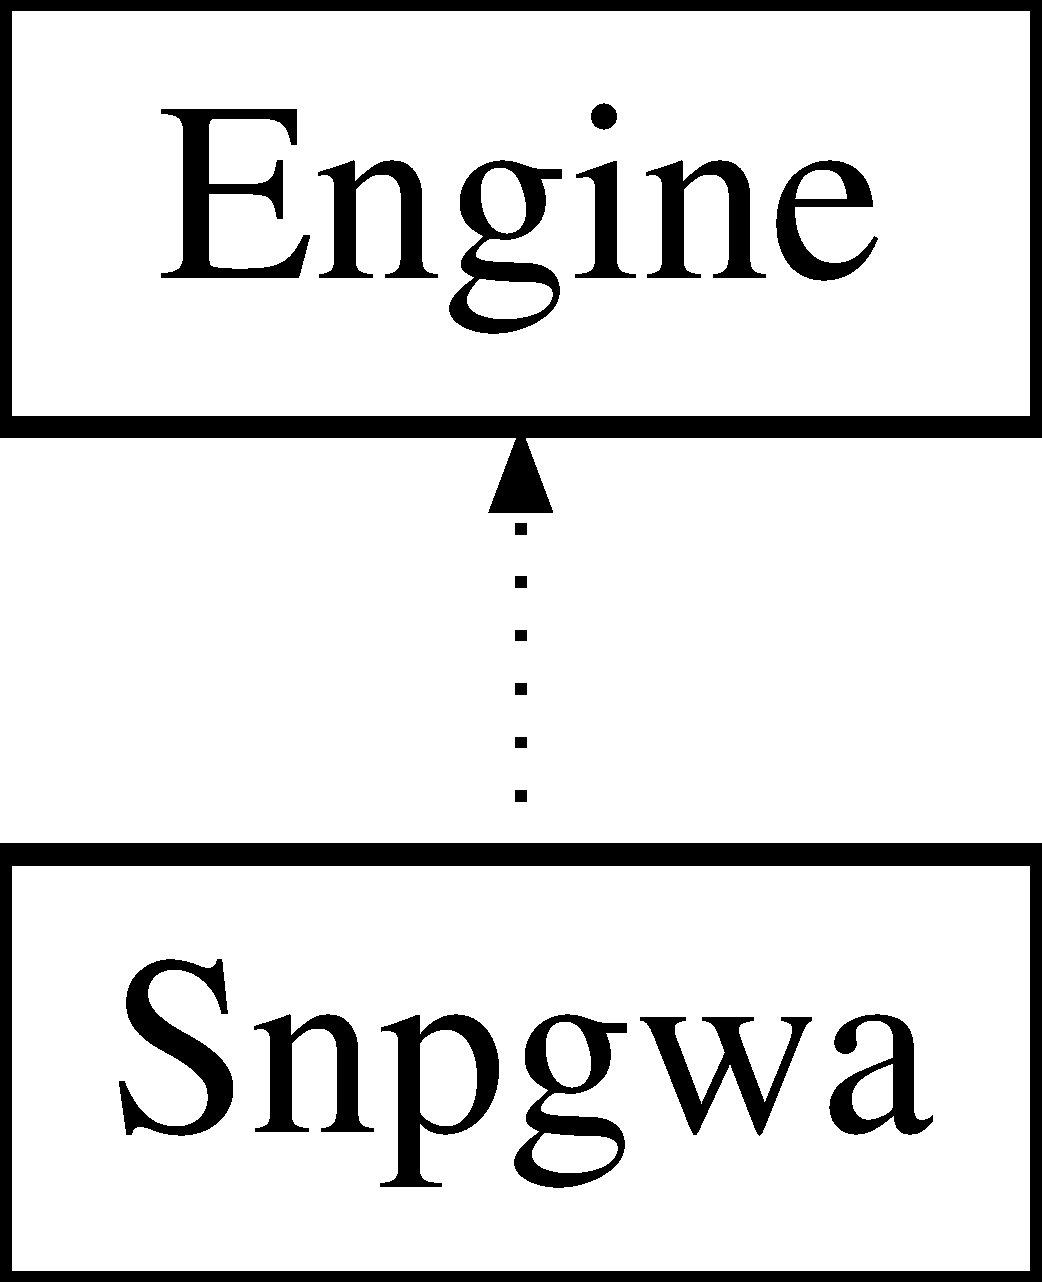
\includegraphics[height=2cm]{classSnpgwa}
\end{center}
\end{figure}
\subsection*{Public Member Functions}
\begin{DoxyCompactItemize}
\item 
\hyperlink{classSnpgwa_af6bc909553a0297002b7863bb8f36b9f}{Snpgwa} ()
\item 
\hyperlink{classSnpgwa_a5c8b9b6f8e59ce1ae40f2a6fe3fbee52}{$\sim$Snpgwa} ()
\item 
virtual void \hyperlink{classSnpgwa_a4d061e98cd1a9b5d9f7d666dea3cd0af}{init} ()
\item 
virtual void \hyperlink{classSnpgwa_aa20dc165d74036ff401ca182f5e980c2}{preProcess} ()
\item 
virtual void \hyperlink{classSnpgwa_a0d01afdbda7f3bb32586962cca76b69a}{process} ()
\item 
virtual void \hyperlink{classSnpgwa_a976e974bf71743c194a9c098cefff04c}{enslave} (\hyperlink{classEngineParamReader}{EngineParamReader} $\ast$)
\item 
virtual void \hyperlink{classSnpgwa_af5ea7279e2d31bc5f05a1fc6cd4ef17e}{test} ()
\end{DoxyCompactItemize}
\subsection*{Protected Member Functions}
\begin{DoxyCompactItemize}
\item 
void \hyperlink{classSnpgwa_ab4eea76f9654a8456bd046213f23d320}{delete\_\-my\_\-innards} ()
\item 
void \hyperlink{classSnpgwa_a5b8b5b406a9ad232ca818dee37d4830d}{initToZero} (\hyperlink{structPopStatsResults}{PopStatsResults} \&p, \hyperlink{structHaploStatsResults}{HaploStatsResults} \&r, \hyperlink{structGenoStatsResults}{GenoStatsResults} \&ge)
\end{DoxyCompactItemize}
\subsection*{Protected Attributes}
\begin{DoxyCompactItemize}
\item 
\hyperlink{classEngineParamReader}{EngineParamReader} $\ast$ \hyperlink{classSnpgwa_a9b2d0153adca8f2c195316160a5f5e6b}{snp\_\-param}
\item 
\hyperlink{classSnpgwaOutput}{SnpgwaOutput} \hyperlink{classSnpgwa_a6c7b080ebb55447368f6f4fc7b6e44b4}{out}
\item 
int \hyperlink{classSnpgwa_ad2186220f31270d57c707e2ab845f805}{numInitSNPs}
\item 
int \hyperlink{classSnpgwa_a8354d2686850eab77dd904721dd274f7}{numInitPhen}
\item 
int \hyperlink{classSnpgwa_a02d3778a5605bd3fa13b2ff48c87382a}{numFinalPhen}
\end{DoxyCompactItemize}


\subsection{Detailed Description}
Main entry point for SNPGWA, a comprehensive single-\/SNP association test suite developed at by Carl Langefeld and group.

Performs tests with both categorical and quantitative phenotypes and with and without covariates.

\begin{DoxyAuthor}{Author}
Richard T. Guy in present form 

Joshua Grab 

Matt Steigert 

Carl D. Langefeld 
\end{DoxyAuthor}


\subsection{Constructor \& Destructor Documentation}
\hypertarget{classSnpgwa_af6bc909553a0297002b7863bb8f36b9f}{
\index{Snpgwa@{Snpgwa}!Snpgwa@{Snpgwa}}
\index{Snpgwa@{Snpgwa}!Snpgwa@{Snpgwa}}
\subsubsection[{Snpgwa}]{\setlength{\rightskip}{0pt plus 5cm}Snpgwa::Snpgwa ()\hspace{0.3cm}{\ttfamily  \mbox{[}explicit\mbox{]}}}}
\label{classSnpgwa_af6bc909553a0297002b7863bb8f36b9f}
\hypertarget{classSnpgwa_a5c8b9b6f8e59ce1ae40f2a6fe3fbee52}{
\index{Snpgwa@{Snpgwa}!$\sim$Snpgwa@{$\sim$Snpgwa}}
\index{$\sim$Snpgwa@{$\sim$Snpgwa}!Snpgwa@{Snpgwa}}
\subsubsection[{$\sim$Snpgwa}]{\setlength{\rightskip}{0pt plus 5cm}Snpgwa::$\sim$Snpgwa ()}}
\label{classSnpgwa_a5c8b9b6f8e59ce1ae40f2a6fe3fbee52}


\subsection{Member Function Documentation}
\hypertarget{classSnpgwa_ab4eea76f9654a8456bd046213f23d320}{
\index{Snpgwa@{Snpgwa}!delete\_\-my\_\-innards@{delete\_\-my\_\-innards}}
\index{delete\_\-my\_\-innards@{delete\_\-my\_\-innards}!Snpgwa@{Snpgwa}}
\subsubsection[{delete\_\-my\_\-innards}]{\setlength{\rightskip}{0pt plus 5cm}void Snpgwa::delete\_\-my\_\-innards ()\hspace{0.3cm}{\ttfamily  \mbox{[}protected\mbox{]}}}}
\label{classSnpgwa_ab4eea76f9654a8456bd046213f23d320}
\hypertarget{classSnpgwa_a976e974bf71743c194a9c098cefff04c}{
\index{Snpgwa@{Snpgwa}!enslave@{enslave}}
\index{enslave@{enslave}!Snpgwa@{Snpgwa}}
\subsubsection[{enslave}]{\setlength{\rightskip}{0pt plus 5cm}void Snpgwa::enslave ({\bf EngineParamReader} $\ast$ {\em e})\hspace{0.3cm}{\ttfamily  \mbox{[}virtual\mbox{]}}}}
\label{classSnpgwa_a976e974bf71743c194a9c098cefff04c}


Implements \hyperlink{classEngine_a023e094182312b1732fe53754c2fe5cb}{Engine}.

\hypertarget{classSnpgwa_a4d061e98cd1a9b5d9f7d666dea3cd0af}{
\index{Snpgwa@{Snpgwa}!init@{init}}
\index{init@{init}!Snpgwa@{Snpgwa}}
\subsubsection[{init}]{\setlength{\rightskip}{0pt plus 5cm}void Snpgwa::init ()\hspace{0.3cm}{\ttfamily  \mbox{[}virtual\mbox{]}}}}
\label{classSnpgwa_a4d061e98cd1a9b5d9f7d666dea3cd0af}
Primary initialization function. Assumes that the parameters have been read and that the data object has not been initialized. Reads data and performs most preprocessing on that data.

After \hyperlink{classSnpgwa_a4d061e98cd1a9b5d9f7d666dea3cd0af}{init()} runs, the data has been loaded and is ready.

Specific tasks: Read data Make categorical Remove individuals missing phenotype. 

Implements \hyperlink{classEngine_aaa054d596fb8ced6e3eb4bee208f8c3d}{Engine}.

\hypertarget{classSnpgwa_a5b8b5b406a9ad232ca818dee37d4830d}{
\index{Snpgwa@{Snpgwa}!initToZero@{initToZero}}
\index{initToZero@{initToZero}!Snpgwa@{Snpgwa}}
\subsubsection[{initToZero}]{\setlength{\rightskip}{0pt plus 5cm}void Snpgwa::initToZero ({\bf PopStatsResults} \& {\em p}, \/  {\bf HaploStatsResults} \& {\em r}, \/  {\bf GenoStatsResults} \& {\em ge})\hspace{0.3cm}{\ttfamily  \mbox{[}protected\mbox{]}}}}
\label{classSnpgwa_a5b8b5b406a9ad232ca818dee37d4830d}
Initialize all members of the group to their default values.


\begin{DoxyParams}{Parameters}
\item[{\em p}]A population results object to be cleared. \item[{\em r}]A HaplotypeStatsResults object to be cleared. \item[{\em ge}]A GenotypeStatsResults object to be cleared. \end{DoxyParams}
\hypertarget{classSnpgwa_aa20dc165d74036ff401ca182f5e980c2}{
\index{Snpgwa@{Snpgwa}!preProcess@{preProcess}}
\index{preProcess@{preProcess}!Snpgwa@{Snpgwa}}
\subsubsection[{preProcess}]{\setlength{\rightskip}{0pt plus 5cm}void Snpgwa::preProcess ()\hspace{0.3cm}{\ttfamily  \mbox{[}virtual\mbox{]}}}}
\label{classSnpgwa_aa20dc165d74036ff401ca182f5e980c2}
Set up output engine, alert user about final data size, and prepare to run tests. 

Implements \hyperlink{classEngine_aec7076b8979a13c96eceb362437dc68c}{Engine}.

\hypertarget{classSnpgwa_a0d01afdbda7f3bb32586962cca76b69a}{
\index{Snpgwa@{Snpgwa}!process@{process}}
\index{process@{process}!Snpgwa@{Snpgwa}}
\subsubsection[{process}]{\setlength{\rightskip}{0pt plus 5cm}void Snpgwa::process ()\hspace{0.3cm}{\ttfamily  \mbox{[}virtual\mbox{]}}}}
\label{classSnpgwa_a0d01afdbda7f3bb32586962cca76b69a}
Primary entry point for SNPgwa processing. Loop through SNPs, potentially in parallel, and write output for each SNP. Utilizes several classes.

\begin{DoxySeeAlso}{See also}
\hyperlink{classPopStats}{PopStats} 

\hyperlink{classGenoStats}{GenoStats} 

\hyperlink{classHaploStats}{HaploStats} 

\hyperlink{classSnpgwaOutput}{SnpgwaOutput} 
\end{DoxySeeAlso}


Implements \hyperlink{classEngine_a005f8e277c3dea16ea05803fba223db7}{Engine}.

\hypertarget{classSnpgwa_af5ea7279e2d31bc5f05a1fc6cd4ef17e}{
\index{Snpgwa@{Snpgwa}!test@{test}}
\index{test@{test}!Snpgwa@{Snpgwa}}
\subsubsection[{test}]{\setlength{\rightskip}{0pt plus 5cm}void Snpgwa::test ()\hspace{0.3cm}{\ttfamily  \mbox{[}virtual\mbox{]}}}}
\label{classSnpgwa_af5ea7279e2d31bc5f05a1fc6cd4ef17e}


Implements \hyperlink{classEngine_a2927c4a4263809453063ad482c6434a4}{Engine}.



\subsection{Field Documentation}
\hypertarget{classSnpgwa_a02d3778a5605bd3fa13b2ff48c87382a}{
\index{Snpgwa@{Snpgwa}!numFinalPhen@{numFinalPhen}}
\index{numFinalPhen@{numFinalPhen}!Snpgwa@{Snpgwa}}
\subsubsection[{numFinalPhen}]{\setlength{\rightskip}{0pt plus 5cm}int {\bf Snpgwa::numFinalPhen}\hspace{0.3cm}{\ttfamily  \mbox{[}protected\mbox{]}}}}
\label{classSnpgwa_a02d3778a5605bd3fa13b2ff48c87382a}
\hypertarget{classSnpgwa_a8354d2686850eab77dd904721dd274f7}{
\index{Snpgwa@{Snpgwa}!numInitPhen@{numInitPhen}}
\index{numInitPhen@{numInitPhen}!Snpgwa@{Snpgwa}}
\subsubsection[{numInitPhen}]{\setlength{\rightskip}{0pt plus 5cm}int {\bf Snpgwa::numInitPhen}\hspace{0.3cm}{\ttfamily  \mbox{[}protected\mbox{]}}}}
\label{classSnpgwa_a8354d2686850eab77dd904721dd274f7}
\hypertarget{classSnpgwa_ad2186220f31270d57c707e2ab845f805}{
\index{Snpgwa@{Snpgwa}!numInitSNPs@{numInitSNPs}}
\index{numInitSNPs@{numInitSNPs}!Snpgwa@{Snpgwa}}
\subsubsection[{numInitSNPs}]{\setlength{\rightskip}{0pt plus 5cm}int {\bf Snpgwa::numInitSNPs}\hspace{0.3cm}{\ttfamily  \mbox{[}protected\mbox{]}}}}
\label{classSnpgwa_ad2186220f31270d57c707e2ab845f805}
\hypertarget{classSnpgwa_a6c7b080ebb55447368f6f4fc7b6e44b4}{
\index{Snpgwa@{Snpgwa}!out@{out}}
\index{out@{out}!Snpgwa@{Snpgwa}}
\subsubsection[{out}]{\setlength{\rightskip}{0pt plus 5cm}{\bf SnpgwaOutput} {\bf Snpgwa::out}\hspace{0.3cm}{\ttfamily  \mbox{[}protected\mbox{]}}}}
\label{classSnpgwa_a6c7b080ebb55447368f6f4fc7b6e44b4}
\hypertarget{classSnpgwa_a9b2d0153adca8f2c195316160a5f5e6b}{
\index{Snpgwa@{Snpgwa}!snp\_\-param@{snp\_\-param}}
\index{snp\_\-param@{snp\_\-param}!Snpgwa@{Snpgwa}}
\subsubsection[{snp\_\-param}]{\setlength{\rightskip}{0pt plus 5cm}{\bf EngineParamReader}$\ast$ {\bf Snpgwa::snp\_\-param}\hspace{0.3cm}{\ttfamily  \mbox{[}protected\mbox{]}}}}
\label{classSnpgwa_a9b2d0153adca8f2c195316160a5f5e6b}


The documentation for this class was generated from the following files:\begin{DoxyCompactItemize}
\item 
engine/snpgwa/\hyperlink{snpgwa_8h}{snpgwa.h}\item 
engine/snpgwa/\hyperlink{snpgwa_8cpp}{snpgwa.cpp}\end{DoxyCompactItemize}

\hypertarget{classSnpgwaOutput}{
\section{SnpgwaOutput Class Reference}
\label{classSnpgwaOutput}\index{SnpgwaOutput@{SnpgwaOutput}}
}


{\ttfamily \#include $<$snpgwa\_\-out.hh$>$}

\subsection*{Public Member Functions}
\begin{DoxyCompactItemize}
\item 
\hyperlink{classSnpgwaOutput_a422139dc18d6a32d36312e35a40a9a1c}{SnpgwaOutput} ()
\item 
\hyperlink{classSnpgwaOutput_af599a28d1b3e2e0b08152c4da3fe5474}{$\sim$SnpgwaOutput} ()
\item 
bool \hyperlink{classSnpgwaOutput_a52e7ec60c5feb78958b62702c5b82918}{init} (\hyperlink{classParamReader}{ParamReader} $\ast$, \hyperlink{classEngineParamReader}{EngineParamReader} $\ast$, int \hyperlink{classSnpgwaOutput_a5c90c26d5435ed4a5315312c8b6fabe5}{maxMapSize}, int numSNPs, string message)
\item 
void \hyperlink{classSnpgwaOutput_a7994a4d439344d2f2839686eba5b0251}{close} ()
\end{DoxyCompactItemize}
\subsection*{Protected Member Functions}
\begin{DoxyCompactItemize}
\item 
void \hyperlink{classSnpgwaOutput_a24ceac8c558ceeee26925f67d64498a4}{writeLine} (int ids, \hyperlink{classSnpInfo}{SnpInfo} \&, const \hyperlink{structPopStatsResults}{PopStatsResults} \&p, const \hyperlink{structHaploStatsResults}{HaploStatsResults} \&h, const \hyperlink{structGenoStatsResults}{GenoStatsResults} \&g)
\item 
void \hyperlink{classSnpgwaOutput_a9af518ccbe41e8cf1a2c91738ed1c5b6}{writeHWELine} (int ids, const \hyperlink{classSnpInfo}{SnpInfo} \&, const \hyperlink{structPopStatsResults}{PopStatsResults} \&p)
\item 
void \hyperlink{classSnpgwaOutput_a303a7331ed885b2f9c400ba25823a8c0}{writeGenoLine} (int idx, const \hyperlink{classSnpInfo}{SnpInfo} \&s, const \hyperlink{structPopStatsResults}{PopStatsResults} \&p, const \hyperlink{structGenoStatsResults}{GenoStatsResults} \&g, const \hyperlink{structHaploStatsResults}{HaploStatsResults} \&h)
\item 
void \hyperlink{classSnpgwaOutput_ae00da2c5932ccf64bb0b69248ae1a9c2}{writeValLine} (int ids, const \hyperlink{classSnpInfo}{SnpInfo} \&, const \hyperlink{structPopStatsResults}{PopStatsResults} \&p, const \hyperlink{structHaploStatsResults}{HaploStatsResults} \&h, const \hyperlink{structGenoStatsResults}{GenoStatsResults} \&g)
\item 
void \hyperlink{classSnpgwaOutput_a090565719776955cc321e83d55693205}{writeHaploLine} (int idx, const \hyperlink{classSnpInfo}{SnpInfo} \&s, const \hyperlink{structHaploStatsResults}{HaploStatsResults} \&p)
\item 
void \hyperlink{classSnpgwaOutput_a0b1354058143385bc05448b3aec6e981}{writeMainHeader} (\hyperlink{classOutput}{Output} \&, \hyperlink{classParamReader}{ParamReader} $\ast$)
\item 
void \hyperlink{classSnpgwaOutput_a60154ce496b7b01f476ac7c2d3056004}{writeMainLegend} (\hyperlink{classOutput}{Output} \&)
\item 
void \hyperlink{classSnpgwaOutput_a2090144186c1c1a6a832c36094661087}{writeHWELegend} (\hyperlink{classOutput}{Output} \&, \hyperlink{classOutput}{Output} \&, \hyperlink{classOutput}{Output} \&)
\item 
void \hyperlink{classSnpgwaOutput_a2499f64888296d1e418175cf4742d506}{writeValLegend} (\hyperlink{classOutput}{Output} \&)
\item 
void \hyperlink{classSnpgwaOutput_a429ecd2ef4d0112dd889b5b36f858ab7}{writeGenoLegend} (\hyperlink{classOutput}{Output} \&o1, \hyperlink{classOutput}{Output} \&o2, \hyperlink{classOutput}{Output} \&o3)
\item 
void \hyperlink{classSnpgwaOutput_a0d4bcf07b492d77a4211ed5ed5fe6397}{writeHaploLegend} (\hyperlink{classOutput}{Output} \&o1, \hyperlink{classOutput}{Output} \&o2, \hyperlink{classOutput}{Output} \&o3)
\item 
void \hyperlink{classSnpgwaOutput_a540b0cec05790adca12054a89ab1b676}{writeLogHead} (\hyperlink{classParamReader}{ParamReader} $\ast$param)
\end{DoxyCompactItemize}
\subsection*{Protected Attributes}
\begin{DoxyCompactItemize}
\item 
\hyperlink{classOutput}{Output} \hyperlink{classSnpgwaOutput_af2ea8e1ff95cb8c724a8efc8056aff36}{outMain}
\item 
\hyperlink{classOutput}{Output} \hyperlink{classSnpgwaOutput_a28b7db56add2bec56ded7839697b41f6}{outGeno1}
\item 
\hyperlink{classOutput}{Output} \hyperlink{classSnpgwaOutput_a9c2018374715ff34aebfcac309962106}{outGeno2}
\item 
\hyperlink{classOutput}{Output} \hyperlink{classSnpgwaOutput_a7dfd380fcf3030f0fecd098cfafde32c}{outGeno3}
\item 
\hyperlink{classOutput}{Output} \hyperlink{classSnpgwaOutput_a9d728bc8033adddfdb54547720f13c73}{outHWEcase}
\item 
\hyperlink{classOutput}{Output} \hyperlink{classSnpgwaOutput_a53257881a705d01c0ab78d025da53d61}{outHWEcntrl}
\item 
\hyperlink{classOutput}{Output} \hyperlink{classSnpgwaOutput_a89f4ca8c3651b9006de67686fa957cfd}{outHWEcomb}
\item 
\hyperlink{classOutput}{Output} \hyperlink{classSnpgwaOutput_aa626994bf9305d3d227b0bbf9f839d7e}{outRefAllele}
\item 
\hyperlink{classOutput}{Output} \hyperlink{classSnpgwaOutput_a243da145889a8533a4cd3031ebe08576}{outHap1}
\item 
\hyperlink{classOutput}{Output} \hyperlink{classSnpgwaOutput_a3a52fcddc649c978401d22f0a30ddab1}{outHap2}
\item 
\hyperlink{classOutput}{Output} \hyperlink{classSnpgwaOutput_ae4caed4f983669568427b957aeb1cf9b}{outHap3}
\item 
\hyperlink{classOutput}{Output} \hyperlink{classSnpgwaOutput_a57f2a586abfd13f34cf89089c21aa449}{outVal}
\item 
int \hyperlink{classSnpgwaOutput_a5c90c26d5435ed4a5315312c8b6fabe5}{maxMapSize}
\item 
int \hyperlink{classSnpgwaOutput_a744eeba177ca22c6b8ab62b4ee62a235}{totalNumSNPs}
\item 
bool \hyperlink{classSnpgwaOutput_a5d21ad5bdb40c49a3f4042f89104ba56}{writeGenoFiles}
\item 
bool \hyperlink{classSnpgwaOutput_a7eb639c3eb44a97ed5bcb4cc39efa3ce}{writeHWEFiles}
\item 
bool \hyperlink{classSnpgwaOutput_aaaf80792184004da79d3fd9f06b800d2}{writeRefFile}
\item 
bool \hyperlink{classSnpgwaOutput_a92dbf1675db0fadf2123a8161df7e75c}{writeValFile}
\item 
bool \hyperlink{classSnpgwaOutput_a755bbf052c1f3936bd8972b78034d01b}{writeHaploFiles}
\item 
bool \hyperlink{classSnpgwaOutput_ac393eff50dde0ea8de38bbc56e05e135}{writeMainFileMap}
\item 
bool \hyperlink{classSnpgwaOutput_ab1081ec8129bf1e0184ab9341653262c}{writeMainFileHap}
\end{DoxyCompactItemize}
\subsection*{Friends}
\begin{DoxyCompactItemize}
\item 
class \hyperlink{classSnpgwaOutput_aa527c01a3a830865c14e42f7d302622d}{Snpgwa}
\end{DoxyCompactItemize}


\subsection{Constructor \& Destructor Documentation}
\hypertarget{classSnpgwaOutput_a422139dc18d6a32d36312e35a40a9a1c}{
\index{SnpgwaOutput@{SnpgwaOutput}!SnpgwaOutput@{SnpgwaOutput}}
\index{SnpgwaOutput@{SnpgwaOutput}!SnpgwaOutput@{SnpgwaOutput}}
\subsubsection[{SnpgwaOutput}]{\setlength{\rightskip}{0pt plus 5cm}SnpgwaOutput::SnpgwaOutput ()}}
\label{classSnpgwaOutput_a422139dc18d6a32d36312e35a40a9a1c}
\hypertarget{classSnpgwaOutput_af599a28d1b3e2e0b08152c4da3fe5474}{
\index{SnpgwaOutput@{SnpgwaOutput}!$\sim$SnpgwaOutput@{$\sim$SnpgwaOutput}}
\index{$\sim$SnpgwaOutput@{$\sim$SnpgwaOutput}!SnpgwaOutput@{SnpgwaOutput}}
\subsubsection[{$\sim$SnpgwaOutput}]{\setlength{\rightskip}{0pt plus 5cm}SnpgwaOutput::$\sim$SnpgwaOutput ()}}
\label{classSnpgwaOutput_af599a28d1b3e2e0b08152c4da3fe5474}


\subsection{Member Function Documentation}
\hypertarget{classSnpgwaOutput_a7994a4d439344d2f2839686eba5b0251}{
\index{SnpgwaOutput@{SnpgwaOutput}!close@{close}}
\index{close@{close}!SnpgwaOutput@{SnpgwaOutput}}
\subsubsection[{close}]{\setlength{\rightskip}{0pt plus 5cm}void SnpgwaOutput::close ()}}
\label{classSnpgwaOutput_a7994a4d439344d2f2839686eba5b0251}
\hypertarget{classSnpgwaOutput_a52e7ec60c5feb78958b62702c5b82918}{
\index{SnpgwaOutput@{SnpgwaOutput}!init@{init}}
\index{init@{init}!SnpgwaOutput@{SnpgwaOutput}}
\subsubsection[{init}]{\setlength{\rightskip}{0pt plus 5cm}bool SnpgwaOutput::init ({\bf ParamReader} $\ast$ {\em param}, \/  {\bf EngineParamReader} $\ast$ {\em eparams}, \/  int {\em maxMapSize}, \/  int {\em numSNPs}, \/  string {\em message})}}
\label{classSnpgwaOutput_a52e7ec60c5feb78958b62702c5b82918}
Initialize all files and write their headers. First, set some variables determining whether some things are even computed.

Use the param object for that.


\begin{DoxyParams}{Parameters}
\item[{\em param}]Parameter store \item[{\em eparams}]\hyperlink{classEngine}{Engine} parameter store. \item[{\em maxMapSize}]The maximum size of a map. \item[{\em numSNPs}]The number of SNPs to be counted. \item[{\em message}]A string message to include between header and legend on the main screen. Will include information on counts, ect.\end{DoxyParams}
\begin{DoxyReturn}{Returns}
bool Successful init. 
\end{DoxyReturn}
\hypertarget{classSnpgwaOutput_a429ecd2ef4d0112dd889b5b36f858ab7}{
\index{SnpgwaOutput@{SnpgwaOutput}!writeGenoLegend@{writeGenoLegend}}
\index{writeGenoLegend@{writeGenoLegend}!SnpgwaOutput@{SnpgwaOutput}}
\subsubsection[{writeGenoLegend}]{\setlength{\rightskip}{0pt plus 5cm}void SnpgwaOutput::writeGenoLegend ({\bf Output} \& {\em o1}, \/  {\bf Output} \& {\em o2}, \/  {\bf Output} \& {\em o3})\hspace{0.3cm}{\ttfamily  \mbox{[}protected\mbox{]}}}}
\label{classSnpgwaOutput_a429ecd2ef4d0112dd889b5b36f858ab7}
Write three legends. \hypertarget{classSnpgwaOutput_a303a7331ed885b2f9c400ba25823a8c0}{
\index{SnpgwaOutput@{SnpgwaOutput}!writeGenoLine@{writeGenoLine}}
\index{writeGenoLine@{writeGenoLine}!SnpgwaOutput@{SnpgwaOutput}}
\subsubsection[{writeGenoLine}]{\setlength{\rightskip}{0pt plus 5cm}void SnpgwaOutput::writeGenoLine (int {\em idx}, \/  const {\bf SnpInfo} \& {\em s}, \/  const {\bf PopStatsResults} \& {\em p}, \/  const {\bf GenoStatsResults} \& {\em g}, \/  const {\bf HaploStatsResults} \& {\em h})\hspace{0.3cm}{\ttfamily  \mbox{[}protected\mbox{]}}}}
\label{classSnpgwaOutput_a303a7331ed885b2f9c400ba25823a8c0}
Write lines for geno files.


\begin{DoxyParams}{Parameters}
\item[{\em idx}]Index in final file (for asynchronous update) \item[{\em s}]Contains SNP info to write. \item[{\em p}]Contains population stats results to write. \item[{\em h}]Contains haplotype stats results to write. \item[{\em g}]Contains genotypic stats results to write. \end{DoxyParams}
\hypertarget{classSnpgwaOutput_a0d4bcf07b492d77a4211ed5ed5fe6397}{
\index{SnpgwaOutput@{SnpgwaOutput}!writeHaploLegend@{writeHaploLegend}}
\index{writeHaploLegend@{writeHaploLegend}!SnpgwaOutput@{SnpgwaOutput}}
\subsubsection[{writeHaploLegend}]{\setlength{\rightskip}{0pt plus 5cm}void SnpgwaOutput::writeHaploLegend ({\bf Output} \& {\em o1}, \/  {\bf Output} \& {\em o2}, \/  {\bf Output} \& {\em o3})\hspace{0.3cm}{\ttfamily  \mbox{[}protected\mbox{]}}}}
\label{classSnpgwaOutput_a0d4bcf07b492d77a4211ed5ed5fe6397}
Write three legends \hypertarget{classSnpgwaOutput_a090565719776955cc321e83d55693205}{
\index{SnpgwaOutput@{SnpgwaOutput}!writeHaploLine@{writeHaploLine}}
\index{writeHaploLine@{writeHaploLine}!SnpgwaOutput@{SnpgwaOutput}}
\subsubsection[{writeHaploLine}]{\setlength{\rightskip}{0pt plus 5cm}void SnpgwaOutput::writeHaploLine (int {\em idx}, \/  const {\bf SnpInfo} \& {\em s}, \/  const {\bf HaploStatsResults} \& {\em p})\hspace{0.3cm}{\ttfamily  \mbox{[}protected\mbox{]}}}}
\label{classSnpgwaOutput_a090565719776955cc321e83d55693205}
\hypertarget{classSnpgwaOutput_a2090144186c1c1a6a832c36094661087}{
\index{SnpgwaOutput@{SnpgwaOutput}!writeHWELegend@{writeHWELegend}}
\index{writeHWELegend@{writeHWELegend}!SnpgwaOutput@{SnpgwaOutput}}
\subsubsection[{writeHWELegend}]{\setlength{\rightskip}{0pt plus 5cm}void SnpgwaOutput::writeHWELegend ({\bf Output} \& {\em outCS}, \/  {\bf Output} \& {\em outCN}, \/  {\bf Output} \& {\em outCB})\hspace{0.3cm}{\ttfamily  \mbox{[}protected\mbox{]}}}}
\label{classSnpgwaOutput_a2090144186c1c1a6a832c36094661087}
\hypertarget{classSnpgwaOutput_a9af518ccbe41e8cf1a2c91738ed1c5b6}{
\index{SnpgwaOutput@{SnpgwaOutput}!writeHWELine@{writeHWELine}}
\index{writeHWELine@{writeHWELine}!SnpgwaOutput@{SnpgwaOutput}}
\subsubsection[{writeHWELine}]{\setlength{\rightskip}{0pt plus 5cm}void SnpgwaOutput::writeHWELine (int {\em idx}, \/  const {\bf SnpInfo} \& {\em s}, \/  const {\bf PopStatsResults} \& {\em p})\hspace{0.3cm}{\ttfamily  \mbox{[}protected\mbox{]}}}}
\label{classSnpgwaOutput_a9af518ccbe41e8cf1a2c91738ed1c5b6}
Write output line to each of the three HWE files.


\begin{DoxyParams}{Parameters}
\item[{\em idx}]Index in final file (for synchronous update) \item[{\em s}]Contains SNP info to write. \item[{\em p}]Contains population stats results to write. \end{DoxyParams}
\hypertarget{classSnpgwaOutput_a24ceac8c558ceeee26925f67d64498a4}{
\index{SnpgwaOutput@{SnpgwaOutput}!writeLine@{writeLine}}
\index{writeLine@{writeLine}!SnpgwaOutput@{SnpgwaOutput}}
\subsubsection[{writeLine}]{\setlength{\rightskip}{0pt plus 5cm}void SnpgwaOutput::writeLine (int {\em idx}, \/  {\bf SnpInfo} \& {\em s}, \/  const {\bf PopStatsResults} \& {\em p}, \/  const {\bf HaploStatsResults} \& {\em h}, \/  const {\bf GenoStatsResults} \& {\em g})\hspace{0.3cm}{\ttfamily  \mbox{[}protected\mbox{]}}}}
\label{classSnpgwaOutput_a24ceac8c558ceeee26925f67d64498a4}
Main writing method.

The structs are created and filled in \hyperlink{snpgwa_8cpp}{snpgwa.cpp}. The index is for parallel creation of an in-\/order output file. It must be 0 based.

The main file is written here. Others are written via calls from here. \hypertarget{classSnpgwaOutput_a540b0cec05790adca12054a89ab1b676}{
\index{SnpgwaOutput@{SnpgwaOutput}!writeLogHead@{writeLogHead}}
\index{writeLogHead@{writeLogHead}!SnpgwaOutput@{SnpgwaOutput}}
\subsubsection[{writeLogHead}]{\setlength{\rightskip}{0pt plus 5cm}void SnpgwaOutput::writeLogHead ({\bf ParamReader} $\ast$ {\em param})\hspace{0.3cm}{\ttfamily  \mbox{[}protected\mbox{]}}}}
\label{classSnpgwaOutput_a540b0cec05790adca12054a89ab1b676}
Write a header to the logging file. \hypertarget{classSnpgwaOutput_a0b1354058143385bc05448b3aec6e981}{
\index{SnpgwaOutput@{SnpgwaOutput}!writeMainHeader@{writeMainHeader}}
\index{writeMainHeader@{writeMainHeader}!SnpgwaOutput@{SnpgwaOutput}}
\subsubsection[{writeMainHeader}]{\setlength{\rightskip}{0pt plus 5cm}void SnpgwaOutput::writeMainHeader ({\bf Output} \& {\em out}, \/  {\bf ParamReader} $\ast$ {\em param})\hspace{0.3cm}{\ttfamily  \mbox{[}protected\mbox{]}}}}
\label{classSnpgwaOutput_a0b1354058143385bc05448b3aec6e981}
\hypertarget{classSnpgwaOutput_a60154ce496b7b01f476ac7c2d3056004}{
\index{SnpgwaOutput@{SnpgwaOutput}!writeMainLegend@{writeMainLegend}}
\index{writeMainLegend@{writeMainLegend}!SnpgwaOutput@{SnpgwaOutput}}
\subsubsection[{writeMainLegend}]{\setlength{\rightskip}{0pt plus 5cm}void SnpgwaOutput::writeMainLegend ({\bf Output} \& {\em out})\hspace{0.3cm}{\ttfamily  \mbox{[}protected\mbox{]}}}}
\label{classSnpgwaOutput_a60154ce496b7b01f476ac7c2d3056004}
Write legend for the main lines. The only decisions that have to be made are whether to print the map file info and whether to print haplo info.

The spacing is very precise this method.


\begin{DoxyParams}{Parameters}
\item[{\em out}]\hyperlink{classOutput}{Output} class object to write to. Utilizes asynchronized output. \end{DoxyParams}
\hypertarget{classSnpgwaOutput_a2499f64888296d1e418175cf4742d506}{
\index{SnpgwaOutput@{SnpgwaOutput}!writeValLegend@{writeValLegend}}
\index{writeValLegend@{writeValLegend}!SnpgwaOutput@{SnpgwaOutput}}
\subsubsection[{writeValLegend}]{\setlength{\rightskip}{0pt plus 5cm}void SnpgwaOutput::writeValLegend ({\bf Output} \& {\em out})\hspace{0.3cm}{\ttfamily  \mbox{[}protected\mbox{]}}}}
\label{classSnpgwaOutput_a2499f64888296d1e418175cf4742d506}
\hypertarget{classSnpgwaOutput_ae00da2c5932ccf64bb0b69248ae1a9c2}{
\index{SnpgwaOutput@{SnpgwaOutput}!writeValLine@{writeValLine}}
\index{writeValLine@{writeValLine}!SnpgwaOutput@{SnpgwaOutput}}
\subsubsection[{writeValLine}]{\setlength{\rightskip}{0pt plus 5cm}void SnpgwaOutput::writeValLine (int {\em ids}, \/  const {\bf SnpInfo} \& {\em s}, \/  const {\bf PopStatsResults} \& {\em p}, \/  const {\bf HaploStatsResults} \& {\em h}, \/  const {\bf GenoStatsResults} \& {\em g})\hspace{0.3cm}{\ttfamily  \mbox{[}protected\mbox{]}}}}
\label{classSnpgwaOutput_ae00da2c5932ccf64bb0b69248ae1a9c2}
Write output line for the value file. This is a separate file that contains test statistics rather than their corresponding p-\/values.


\begin{DoxyParams}{Parameters}
\item[{\em ids}]Index in final file (for asynchronous update) \item[{\em s}]Contains SNP info to write. \item[{\em p}]Contains population stats results to write. \item[{\em h}]Contains haplotype stats results to write. \item[{\em g}]Contains genotypic stats results to write. \end{DoxyParams}


\subsection{Friends And Related Function Documentation}
\hypertarget{classSnpgwaOutput_aa527c01a3a830865c14e42f7d302622d}{
\index{SnpgwaOutput@{SnpgwaOutput}!Snpgwa@{Snpgwa}}
\index{Snpgwa@{Snpgwa}!SnpgwaOutput@{SnpgwaOutput}}
\subsubsection[{Snpgwa}]{\setlength{\rightskip}{0pt plus 5cm}friend class {\bf Snpgwa}\hspace{0.3cm}{\ttfamily  \mbox{[}friend\mbox{]}}}}
\label{classSnpgwaOutput_aa527c01a3a830865c14e42f7d302622d}


\subsection{Field Documentation}
\hypertarget{classSnpgwaOutput_a5c90c26d5435ed4a5315312c8b6fabe5}{
\index{SnpgwaOutput@{SnpgwaOutput}!maxMapSize@{maxMapSize}}
\index{maxMapSize@{maxMapSize}!SnpgwaOutput@{SnpgwaOutput}}
\subsubsection[{maxMapSize}]{\setlength{\rightskip}{0pt plus 5cm}int {\bf SnpgwaOutput::maxMapSize}\hspace{0.3cm}{\ttfamily  \mbox{[}protected\mbox{]}}}}
\label{classSnpgwaOutput_a5c90c26d5435ed4a5315312c8b6fabe5}
\hypertarget{classSnpgwaOutput_a28b7db56add2bec56ded7839697b41f6}{
\index{SnpgwaOutput@{SnpgwaOutput}!outGeno1@{outGeno1}}
\index{outGeno1@{outGeno1}!SnpgwaOutput@{SnpgwaOutput}}
\subsubsection[{outGeno1}]{\setlength{\rightskip}{0pt plus 5cm}{\bf Output} {\bf SnpgwaOutput::outGeno1}\hspace{0.3cm}{\ttfamily  \mbox{[}protected\mbox{]}}}}
\label{classSnpgwaOutput_a28b7db56add2bec56ded7839697b41f6}
\hypertarget{classSnpgwaOutput_a9c2018374715ff34aebfcac309962106}{
\index{SnpgwaOutput@{SnpgwaOutput}!outGeno2@{outGeno2}}
\index{outGeno2@{outGeno2}!SnpgwaOutput@{SnpgwaOutput}}
\subsubsection[{outGeno2}]{\setlength{\rightskip}{0pt plus 5cm}{\bf Output} {\bf SnpgwaOutput::outGeno2}\hspace{0.3cm}{\ttfamily  \mbox{[}protected\mbox{]}}}}
\label{classSnpgwaOutput_a9c2018374715ff34aebfcac309962106}
\hypertarget{classSnpgwaOutput_a7dfd380fcf3030f0fecd098cfafde32c}{
\index{SnpgwaOutput@{SnpgwaOutput}!outGeno3@{outGeno3}}
\index{outGeno3@{outGeno3}!SnpgwaOutput@{SnpgwaOutput}}
\subsubsection[{outGeno3}]{\setlength{\rightskip}{0pt plus 5cm}{\bf Output} {\bf SnpgwaOutput::outGeno3}\hspace{0.3cm}{\ttfamily  \mbox{[}protected\mbox{]}}}}
\label{classSnpgwaOutput_a7dfd380fcf3030f0fecd098cfafde32c}
\hypertarget{classSnpgwaOutput_a243da145889a8533a4cd3031ebe08576}{
\index{SnpgwaOutput@{SnpgwaOutput}!outHap1@{outHap1}}
\index{outHap1@{outHap1}!SnpgwaOutput@{SnpgwaOutput}}
\subsubsection[{outHap1}]{\setlength{\rightskip}{0pt plus 5cm}{\bf Output} {\bf SnpgwaOutput::outHap1}\hspace{0.3cm}{\ttfamily  \mbox{[}protected\mbox{]}}}}
\label{classSnpgwaOutput_a243da145889a8533a4cd3031ebe08576}
\hypertarget{classSnpgwaOutput_a3a52fcddc649c978401d22f0a30ddab1}{
\index{SnpgwaOutput@{SnpgwaOutput}!outHap2@{outHap2}}
\index{outHap2@{outHap2}!SnpgwaOutput@{SnpgwaOutput}}
\subsubsection[{outHap2}]{\setlength{\rightskip}{0pt plus 5cm}{\bf Output} {\bf SnpgwaOutput::outHap2}\hspace{0.3cm}{\ttfamily  \mbox{[}protected\mbox{]}}}}
\label{classSnpgwaOutput_a3a52fcddc649c978401d22f0a30ddab1}
\hypertarget{classSnpgwaOutput_ae4caed4f983669568427b957aeb1cf9b}{
\index{SnpgwaOutput@{SnpgwaOutput}!outHap3@{outHap3}}
\index{outHap3@{outHap3}!SnpgwaOutput@{SnpgwaOutput}}
\subsubsection[{outHap3}]{\setlength{\rightskip}{0pt plus 5cm}{\bf Output} {\bf SnpgwaOutput::outHap3}\hspace{0.3cm}{\ttfamily  \mbox{[}protected\mbox{]}}}}
\label{classSnpgwaOutput_ae4caed4f983669568427b957aeb1cf9b}
\hypertarget{classSnpgwaOutput_a9d728bc8033adddfdb54547720f13c73}{
\index{SnpgwaOutput@{SnpgwaOutput}!outHWEcase@{outHWEcase}}
\index{outHWEcase@{outHWEcase}!SnpgwaOutput@{SnpgwaOutput}}
\subsubsection[{outHWEcase}]{\setlength{\rightskip}{0pt plus 5cm}{\bf Output} {\bf SnpgwaOutput::outHWEcase}\hspace{0.3cm}{\ttfamily  \mbox{[}protected\mbox{]}}}}
\label{classSnpgwaOutput_a9d728bc8033adddfdb54547720f13c73}
\hypertarget{classSnpgwaOutput_a53257881a705d01c0ab78d025da53d61}{
\index{SnpgwaOutput@{SnpgwaOutput}!outHWEcntrl@{outHWEcntrl}}
\index{outHWEcntrl@{outHWEcntrl}!SnpgwaOutput@{SnpgwaOutput}}
\subsubsection[{outHWEcntrl}]{\setlength{\rightskip}{0pt plus 5cm}{\bf Output} {\bf SnpgwaOutput::outHWEcntrl}\hspace{0.3cm}{\ttfamily  \mbox{[}protected\mbox{]}}}}
\label{classSnpgwaOutput_a53257881a705d01c0ab78d025da53d61}
\hypertarget{classSnpgwaOutput_a89f4ca8c3651b9006de67686fa957cfd}{
\index{SnpgwaOutput@{SnpgwaOutput}!outHWEcomb@{outHWEcomb}}
\index{outHWEcomb@{outHWEcomb}!SnpgwaOutput@{SnpgwaOutput}}
\subsubsection[{outHWEcomb}]{\setlength{\rightskip}{0pt plus 5cm}{\bf Output} {\bf SnpgwaOutput::outHWEcomb}\hspace{0.3cm}{\ttfamily  \mbox{[}protected\mbox{]}}}}
\label{classSnpgwaOutput_a89f4ca8c3651b9006de67686fa957cfd}
\hypertarget{classSnpgwaOutput_af2ea8e1ff95cb8c724a8efc8056aff36}{
\index{SnpgwaOutput@{SnpgwaOutput}!outMain@{outMain}}
\index{outMain@{outMain}!SnpgwaOutput@{SnpgwaOutput}}
\subsubsection[{outMain}]{\setlength{\rightskip}{0pt plus 5cm}{\bf Output} {\bf SnpgwaOutput::outMain}\hspace{0.3cm}{\ttfamily  \mbox{[}protected\mbox{]}}}}
\label{classSnpgwaOutput_af2ea8e1ff95cb8c724a8efc8056aff36}
\hypertarget{classSnpgwaOutput_aa626994bf9305d3d227b0bbf9f839d7e}{
\index{SnpgwaOutput@{SnpgwaOutput}!outRefAllele@{outRefAllele}}
\index{outRefAllele@{outRefAllele}!SnpgwaOutput@{SnpgwaOutput}}
\subsubsection[{outRefAllele}]{\setlength{\rightskip}{0pt plus 5cm}{\bf Output} {\bf SnpgwaOutput::outRefAllele}\hspace{0.3cm}{\ttfamily  \mbox{[}protected\mbox{]}}}}
\label{classSnpgwaOutput_aa626994bf9305d3d227b0bbf9f839d7e}
\hypertarget{classSnpgwaOutput_a57f2a586abfd13f34cf89089c21aa449}{
\index{SnpgwaOutput@{SnpgwaOutput}!outVal@{outVal}}
\index{outVal@{outVal}!SnpgwaOutput@{SnpgwaOutput}}
\subsubsection[{outVal}]{\setlength{\rightskip}{0pt plus 5cm}{\bf Output} {\bf SnpgwaOutput::outVal}\hspace{0.3cm}{\ttfamily  \mbox{[}protected\mbox{]}}}}
\label{classSnpgwaOutput_a57f2a586abfd13f34cf89089c21aa449}
\hypertarget{classSnpgwaOutput_a744eeba177ca22c6b8ab62b4ee62a235}{
\index{SnpgwaOutput@{SnpgwaOutput}!totalNumSNPs@{totalNumSNPs}}
\index{totalNumSNPs@{totalNumSNPs}!SnpgwaOutput@{SnpgwaOutput}}
\subsubsection[{totalNumSNPs}]{\setlength{\rightskip}{0pt plus 5cm}int {\bf SnpgwaOutput::totalNumSNPs}\hspace{0.3cm}{\ttfamily  \mbox{[}protected\mbox{]}}}}
\label{classSnpgwaOutput_a744eeba177ca22c6b8ab62b4ee62a235}
\hypertarget{classSnpgwaOutput_a5d21ad5bdb40c49a3f4042f89104ba56}{
\index{SnpgwaOutput@{SnpgwaOutput}!writeGenoFiles@{writeGenoFiles}}
\index{writeGenoFiles@{writeGenoFiles}!SnpgwaOutput@{SnpgwaOutput}}
\subsubsection[{writeGenoFiles}]{\setlength{\rightskip}{0pt plus 5cm}bool {\bf SnpgwaOutput::writeGenoFiles}\hspace{0.3cm}{\ttfamily  \mbox{[}protected\mbox{]}}}}
\label{classSnpgwaOutput_a5d21ad5bdb40c49a3f4042f89104ba56}
\hypertarget{classSnpgwaOutput_a755bbf052c1f3936bd8972b78034d01b}{
\index{SnpgwaOutput@{SnpgwaOutput}!writeHaploFiles@{writeHaploFiles}}
\index{writeHaploFiles@{writeHaploFiles}!SnpgwaOutput@{SnpgwaOutput}}
\subsubsection[{writeHaploFiles}]{\setlength{\rightskip}{0pt plus 5cm}bool {\bf SnpgwaOutput::writeHaploFiles}\hspace{0.3cm}{\ttfamily  \mbox{[}protected\mbox{]}}}}
\label{classSnpgwaOutput_a755bbf052c1f3936bd8972b78034d01b}
\hypertarget{classSnpgwaOutput_a7eb639c3eb44a97ed5bcb4cc39efa3ce}{
\index{SnpgwaOutput@{SnpgwaOutput}!writeHWEFiles@{writeHWEFiles}}
\index{writeHWEFiles@{writeHWEFiles}!SnpgwaOutput@{SnpgwaOutput}}
\subsubsection[{writeHWEFiles}]{\setlength{\rightskip}{0pt plus 5cm}bool {\bf SnpgwaOutput::writeHWEFiles}\hspace{0.3cm}{\ttfamily  \mbox{[}protected\mbox{]}}}}
\label{classSnpgwaOutput_a7eb639c3eb44a97ed5bcb4cc39efa3ce}
\hypertarget{classSnpgwaOutput_ab1081ec8129bf1e0184ab9341653262c}{
\index{SnpgwaOutput@{SnpgwaOutput}!writeMainFileHap@{writeMainFileHap}}
\index{writeMainFileHap@{writeMainFileHap}!SnpgwaOutput@{SnpgwaOutput}}
\subsubsection[{writeMainFileHap}]{\setlength{\rightskip}{0pt plus 5cm}bool {\bf SnpgwaOutput::writeMainFileHap}\hspace{0.3cm}{\ttfamily  \mbox{[}protected\mbox{]}}}}
\label{classSnpgwaOutput_ab1081ec8129bf1e0184ab9341653262c}
\hypertarget{classSnpgwaOutput_ac393eff50dde0ea8de38bbc56e05e135}{
\index{SnpgwaOutput@{SnpgwaOutput}!writeMainFileMap@{writeMainFileMap}}
\index{writeMainFileMap@{writeMainFileMap}!SnpgwaOutput@{SnpgwaOutput}}
\subsubsection[{writeMainFileMap}]{\setlength{\rightskip}{0pt plus 5cm}bool {\bf SnpgwaOutput::writeMainFileMap}\hspace{0.3cm}{\ttfamily  \mbox{[}protected\mbox{]}}}}
\label{classSnpgwaOutput_ac393eff50dde0ea8de38bbc56e05e135}
\hypertarget{classSnpgwaOutput_aaaf80792184004da79d3fd9f06b800d2}{
\index{SnpgwaOutput@{SnpgwaOutput}!writeRefFile@{writeRefFile}}
\index{writeRefFile@{writeRefFile}!SnpgwaOutput@{SnpgwaOutput}}
\subsubsection[{writeRefFile}]{\setlength{\rightskip}{0pt plus 5cm}bool {\bf SnpgwaOutput::writeRefFile}\hspace{0.3cm}{\ttfamily  \mbox{[}protected\mbox{]}}}}
\label{classSnpgwaOutput_aaaf80792184004da79d3fd9f06b800d2}
\hypertarget{classSnpgwaOutput_a92dbf1675db0fadf2123a8161df7e75c}{
\index{SnpgwaOutput@{SnpgwaOutput}!writeValFile@{writeValFile}}
\index{writeValFile@{writeValFile}!SnpgwaOutput@{SnpgwaOutput}}
\subsubsection[{writeValFile}]{\setlength{\rightskip}{0pt plus 5cm}bool {\bf SnpgwaOutput::writeValFile}\hspace{0.3cm}{\ttfamily  \mbox{[}protected\mbox{]}}}}
\label{classSnpgwaOutput_a92dbf1675db0fadf2123a8161df7e75c}


The documentation for this class was generated from the following files:\begin{DoxyCompactItemize}
\item 
engine/output/\hyperlink{snpgwa__out_8hh}{snpgwa\_\-out.hh}\item 
engine/output/\hyperlink{snpgwa__out_8cpp}{snpgwa\_\-out.cpp}\end{DoxyCompactItemize}

\hypertarget{classSnpInfo}{
\section{SnpInfo Class Reference}
\label{classSnpInfo}\index{SnpInfo@{SnpInfo}}
}


{\ttfamily \#include $<$snpinfo\_\-out.hh$>$}

\subsection*{Public Member Functions}
\begin{DoxyCompactItemize}
\item 
\hyperlink{classSnpInfo_a65b651b47027f6f55b082b063a183471}{SnpInfo} ()
\item 
void \hyperlink{classSnpInfo_aadc0bad527f131f3294847b552241f32}{print} (std::ostream \&ss, int maxMapSize, bool printMap=true)
\end{DoxyCompactItemize}
\subsection*{Data Fields}
\begin{DoxyCompactItemize}
\item 
int \hyperlink{classSnpInfo_a9e340750436d460a79d14a3cca98d4c2}{index}
\item 
std::string \hyperlink{classSnpInfo_a0eda22dd7438af3aed0ff4a6ed66c5a2}{name}
\item 
int \hyperlink{classSnpInfo_a591c2bc650f6108b2e6ce0088ca1c8ca}{position}
\item 
int \hyperlink{classSnpInfo_a8703dc63736fd564b6d0f2f7c133fb51}{diff}
\item 
std::string \hyperlink{classSnpInfo_afa65e7acd26e25091182b52b2d8fdeab}{chr}
\item 
char \hyperlink{classSnpInfo_a81ef1a04ce03dbcbd357081f2f9da5bc}{majAllele}
\item 
char \hyperlink{classSnpInfo_a9dbfcbe8817b01358436533774b1d36b}{minAllele}
\item 
char \hyperlink{classSnpInfo_a7bb6397cd3bbc9461b0b2bf5390bf2b1}{refAllele}
\end{DoxyCompactItemize}


\subsection{Detailed Description}
Holds snp information that is used in several program outputs. 

\subsection{Constructor \& Destructor Documentation}
\hypertarget{classSnpInfo_a65b651b47027f6f55b082b063a183471}{
\index{SnpInfo@{SnpInfo}!SnpInfo@{SnpInfo}}
\index{SnpInfo@{SnpInfo}!SnpInfo@{SnpInfo}}
\subsubsection[{SnpInfo}]{\setlength{\rightskip}{0pt plus 5cm}SnpInfo::SnpInfo ()}}
\label{classSnpInfo_a65b651b47027f6f55b082b063a183471}


\subsection{Member Function Documentation}
\hypertarget{classSnpInfo_aadc0bad527f131f3294847b552241f32}{
\index{SnpInfo@{SnpInfo}!print@{print}}
\index{print@{print}!SnpInfo@{SnpInfo}}
\subsubsection[{print}]{\setlength{\rightskip}{0pt plus 5cm}void SnpInfo::print (std::ostream \& {\em ss}, \/  int {\em maxMapSize}, \/  bool {\em printMap} = {\ttfamily true})}}
\label{classSnpInfo_aadc0bad527f131f3294847b552241f32}


\subsection{Field Documentation}
\hypertarget{classSnpInfo_afa65e7acd26e25091182b52b2d8fdeab}{
\index{SnpInfo@{SnpInfo}!chr@{chr}}
\index{chr@{chr}!SnpInfo@{SnpInfo}}
\subsubsection[{chr}]{\setlength{\rightskip}{0pt plus 5cm}std::string {\bf SnpInfo::chr}}}
\label{classSnpInfo_afa65e7acd26e25091182b52b2d8fdeab}
\hypertarget{classSnpInfo_a8703dc63736fd564b6d0f2f7c133fb51}{
\index{SnpInfo@{SnpInfo}!diff@{diff}}
\index{diff@{diff}!SnpInfo@{SnpInfo}}
\subsubsection[{diff}]{\setlength{\rightskip}{0pt plus 5cm}int {\bf SnpInfo::diff}}}
\label{classSnpInfo_a8703dc63736fd564b6d0f2f7c133fb51}
\hypertarget{classSnpInfo_a9e340750436d460a79d14a3cca98d4c2}{
\index{SnpInfo@{SnpInfo}!index@{index}}
\index{index@{index}!SnpInfo@{SnpInfo}}
\subsubsection[{index}]{\setlength{\rightskip}{0pt plus 5cm}int {\bf SnpInfo::index}}}
\label{classSnpInfo_a9e340750436d460a79d14a3cca98d4c2}
\hypertarget{classSnpInfo_a81ef1a04ce03dbcbd357081f2f9da5bc}{
\index{SnpInfo@{SnpInfo}!majAllele@{majAllele}}
\index{majAllele@{majAllele}!SnpInfo@{SnpInfo}}
\subsubsection[{majAllele}]{\setlength{\rightskip}{0pt plus 5cm}char {\bf SnpInfo::majAllele}}}
\label{classSnpInfo_a81ef1a04ce03dbcbd357081f2f9da5bc}
\hypertarget{classSnpInfo_a9dbfcbe8817b01358436533774b1d36b}{
\index{SnpInfo@{SnpInfo}!minAllele@{minAllele}}
\index{minAllele@{minAllele}!SnpInfo@{SnpInfo}}
\subsubsection[{minAllele}]{\setlength{\rightskip}{0pt plus 5cm}char {\bf SnpInfo::minAllele}}}
\label{classSnpInfo_a9dbfcbe8817b01358436533774b1d36b}
\hypertarget{classSnpInfo_a0eda22dd7438af3aed0ff4a6ed66c5a2}{
\index{SnpInfo@{SnpInfo}!name@{name}}
\index{name@{name}!SnpInfo@{SnpInfo}}
\subsubsection[{name}]{\setlength{\rightskip}{0pt plus 5cm}std::string {\bf SnpInfo::name}}}
\label{classSnpInfo_a0eda22dd7438af3aed0ff4a6ed66c5a2}
\hypertarget{classSnpInfo_a591c2bc650f6108b2e6ce0088ca1c8ca}{
\index{SnpInfo@{SnpInfo}!position@{position}}
\index{position@{position}!SnpInfo@{SnpInfo}}
\subsubsection[{position}]{\setlength{\rightskip}{0pt plus 5cm}int {\bf SnpInfo::position}}}
\label{classSnpInfo_a591c2bc650f6108b2e6ce0088ca1c8ca}
\hypertarget{classSnpInfo_a7bb6397cd3bbc9461b0b2bf5390bf2b1}{
\index{SnpInfo@{SnpInfo}!refAllele@{refAllele}}
\index{refAllele@{refAllele}!SnpInfo@{SnpInfo}}
\subsubsection[{refAllele}]{\setlength{\rightskip}{0pt plus 5cm}char {\bf SnpInfo::refAllele}}}
\label{classSnpInfo_a7bb6397cd3bbc9461b0b2bf5390bf2b1}


The documentation for this class was generated from the following files:\begin{DoxyCompactItemize}
\item 
engine/output/\hyperlink{snpinfo__out_8hh}{snpinfo\_\-out.hh}\item 
engine/output/\hyperlink{snpinfo__out_8cpp}{snpinfo\_\-out.cpp}\end{DoxyCompactItemize}

\hypertarget{classStatistics}{
\section{Statistics Class Reference}
\label{classStatistics}\index{Statistics@{Statistics}}
}


{\ttfamily \#include $<$statistics.h$>$}

\subsection*{Static Public Member Functions}
\begin{DoxyCompactItemize}
\item 
static double \hyperlink{classStatistics_a7577018477349241f3c5ae3760590aee}{chi2prob} (double chi2val, double df)
\item 
static double \hyperlink{classStatistics_a024e673ac44377b48a9744481d6edc96}{normalPValue} (double value)
\item 
static double \hyperlink{classStatistics_a16ece213e64bb53a786cb4171efe2290}{tdist} (double t, int df)
\item 
static double \hyperlink{classStatistics_a2b6ee0e84409d64cd26377258750c61b}{fdist} (double x, int mval, int nval)
\item 
static double \hyperlink{classStatistics_a2354707a932318f80943bd0a197f0055}{gammq} (double, double)
\begin{DoxyCompactList}\small\item\em Helpers for chi2prob. \item\end{DoxyCompactList}\item 
static void \hyperlink{classStatistics_a6f2de659aa389b60e2de44070f1fc467}{gser} (double $\ast$, double, double, double $\ast$)
\item 
static void \hyperlink{classStatistics_a7c05e92e684944e4e24adb04f64dfc74}{gcf} (double $\ast$, double, double, double $\ast$)
\item 
static double \hyperlink{classStatistics_ad1340b8f52570bb39f6fae2a565e4a90}{gammln} (double)
\item 
static double \hyperlink{classStatistics_a7802e672039a0e6d879333ed83bb53a4}{gamma\_\-log} (double x)
\item 
static double \hyperlink{classStatistics_a125d2cca3291146c2623f3fcc4a16b43}{normal\_\-01\_\-cdf} (double x)
\item 
static double \hyperlink{classStatistics_af33851046a60580f5c9b75db34f444bf}{ITMAX} ()
\item 
static double \hyperlink{classStatistics_a5ad507e0d20b4af70a7691d6ad0ef1a0}{EPS} ()
\item 
static double \hyperlink{classStatistics_a5ba99c9fa2e04ab87c0bb9fb82b36971}{beta\_\-inc} (double a, double b, double x)
\begin{DoxyCompactList}\small\item\em Helpers for Tdist. \item\end{DoxyCompactList}\item 
static double \hyperlink{classStatistics_a8117a4ebebc8b50c8d3dde0b7d2bc859}{beta} (double x, double y)
\item 
static double \hyperlink{classStatistics_a51af50a7c894127977d718981c54b728}{d\_\-epsilon} ()
\begin{DoxyCompactList}\small\item\em General utilities. \item\end{DoxyCompactList}\item 
static void \hyperlink{classStatistics_a7d81d74eba1f1708c0c794f7f2a47b5e}{runAllTests} ()
\begin{DoxyCompactList}\small\item\em Test code. \item\end{DoxyCompactList}\item 
static void \hyperlink{classStatistics_a35a1a03a8cd3ffe80c09518d1972f148}{test\_\-beta\_\-inc} ()
\end{DoxyCompactItemize}


\subsection{Detailed Description}
\begin{DoxyAuthor}{Author}
Unknown, Aggregated by Richard T. Guy
\end{DoxyAuthor}
Static class contains statistical tools.

Current tool set:

Chi2Prob 

\subsection{Member Function Documentation}
\hypertarget{classStatistics_a8117a4ebebc8b50c8d3dde0b7d2bc859}{
\index{Statistics@{Statistics}!beta@{beta}}
\index{beta@{beta}!Statistics@{Statistics}}
\subsubsection[{beta}]{\setlength{\rightskip}{0pt plus 5cm}double Statistics::beta (double {\em x}, \/  double {\em y})\hspace{0.3cm}{\ttfamily  \mbox{[}static\mbox{]}}}}
\label{classStatistics_a8117a4ebebc8b50c8d3dde0b7d2bc859}
Return value of beta function.

\begin{DoxyAuthor}{Author}
Matt Steigart ?
\end{DoxyAuthor}

\begin{DoxyParams}{Parameters}
\item[{\em x}]\item[{\em y}]\end{DoxyParams}
\begin{DoxyReturn}{Returns}
double 
\end{DoxyReturn}
\hypertarget{classStatistics_a5ba99c9fa2e04ab87c0bb9fb82b36971}{
\index{Statistics@{Statistics}!beta\_\-inc@{beta\_\-inc}}
\index{beta\_\-inc@{beta\_\-inc}!Statistics@{Statistics}}
\subsubsection[{beta\_\-inc}]{\setlength{\rightskip}{0pt plus 5cm}double Statistics::beta\_\-inc (double {\em a}, \/  double {\em b}, \/  double {\em x})\hspace{0.3cm}{\ttfamily  \mbox{[}static\mbox{]}}}}
\label{classStatistics_a5ba99c9fa2e04ab87c0bb9fb82b36971}


Helpers for Tdist. 

Return value of incomplete beta function.

\begin{DoxyAuthor}{Author}
Matt Steigart?
\end{DoxyAuthor}

\begin{DoxyParams}{Parameters}
\item[{\em a}]\item[{\em b}]\item[{\em x}]\end{DoxyParams}
\begin{DoxyReturn}{Returns}
double 
\end{DoxyReturn}
\hypertarget{classStatistics_a7577018477349241f3c5ae3760590aee}{
\index{Statistics@{Statistics}!chi2prob@{chi2prob}}
\index{chi2prob@{chi2prob}!Statistics@{Statistics}}
\subsubsection[{chi2prob}]{\setlength{\rightskip}{0pt plus 5cm}double Statistics::chi2prob (double {\em x2val}, \/  double {\em df})\hspace{0.3cm}{\ttfamily  \mbox{[}static\mbox{]}}}}
\label{classStatistics_a7577018477349241f3c5ae3760590aee}
Convert a chi$^\wedge$2 value with a given number of degrees of freedom to a p-\/value.

Throws EX\_\-INVALID\_\-CHI\_\-SQUARE EX\_\-GAMMA\_\-FXN\_\-FAILURE

Convert a chi$^\wedge$2 value with a given number of degrees of freedom to a p-\/value.

\begin{DoxyAuthor}{Author}
Matt Steigert 
\end{DoxyAuthor}

\begin{DoxyParams}{Parameters}
\item[{\em x2val}]The chi$^\wedge$2 distributed statistic \item[{\em df}]Degrees of freedom \end{DoxyParams}
\begin{DoxyReturn}{Returns}
Value of chi2(x2val, df)
\end{DoxyReturn}

\begin{DoxyExceptions}{Exceptions}
\item[{\em InvalidChiSquareException()}]If df $<$ 1 or x2val $<$ 0.0 \end{DoxyExceptions}
\hypertarget{classStatistics_a51af50a7c894127977d718981c54b728}{
\index{Statistics@{Statistics}!d\_\-epsilon@{d\_\-epsilon}}
\index{d\_\-epsilon@{d\_\-epsilon}!Statistics@{Statistics}}
\subsubsection[{d\_\-epsilon}]{\setlength{\rightskip}{0pt plus 5cm}double Statistics::d\_\-epsilon ()\hspace{0.3cm}{\ttfamily  \mbox{[}static\mbox{]}}}}
\label{classStatistics_a51af50a7c894127977d718981c54b728}


General utilities. 

Return roundoff error: the smallest number of form 1 / 2$^\wedge$k different from one.

\begin{DoxyReturn}{Returns}
r -\/ Roundoff size. 
\end{DoxyReturn}
\hypertarget{classStatistics_a5ad507e0d20b4af70a7691d6ad0ef1a0}{
\index{Statistics@{Statistics}!EPS@{EPS}}
\index{EPS@{EPS}!Statistics@{Statistics}}
\subsubsection[{EPS}]{\setlength{\rightskip}{0pt plus 5cm}static double Statistics::EPS ()\hspace{0.3cm}{\ttfamily  \mbox{[}inline, static\mbox{]}}}}
\label{classStatistics_a5ad507e0d20b4af70a7691d6ad0ef1a0}
\hypertarget{classStatistics_a2b6ee0e84409d64cd26377258750c61b}{
\index{Statistics@{Statistics}!fdist@{fdist}}
\index{fdist@{fdist}!Statistics@{Statistics}}
\subsubsection[{fdist}]{\setlength{\rightskip}{0pt plus 5cm}double Statistics::fdist (double {\em x}, \/  int {\em mval}, \/  int {\em nval})\hspace{0.3cm}{\ttfamily  \mbox{[}static\mbox{]}}}}
\label{classStatistics_a2b6ee0e84409d64cd26377258750c61b}
Compute f-\/statistic for a given input.

\begin{DoxyAuthor}{Author}
Matt Steiger
\end{DoxyAuthor}

\begin{DoxyParams}{Parameters}
\item[{\em x}]The test statistic \item[{\em mval}]Degrees of freedom explained \item[{\em nval}]Degrees of freedom unexplained. \end{DoxyParams}
\begin{DoxyReturn}{Returns}
double The probability under the F(mval,nval) of observing x or less extreme. 
\end{DoxyReturn}
\hypertarget{classStatistics_a7802e672039a0e6d879333ed83bb53a4}{
\index{Statistics@{Statistics}!gamma\_\-log@{gamma\_\-log}}
\index{gamma\_\-log@{gamma\_\-log}!Statistics@{Statistics}}
\subsubsection[{gamma\_\-log}]{\setlength{\rightskip}{0pt plus 5cm}double Statistics::gamma\_\-log (double {\em x})\hspace{0.3cm}{\ttfamily  \mbox{[}static\mbox{]}}}}
\label{classStatistics_a7802e672039a0e6d879333ed83bb53a4}
Compute natural log of the gamma function.


\begin{DoxyParams}{Parameters}
\item[{\em x}]\end{DoxyParams}
\begin{DoxyReturn}{Returns}
double 
\end{DoxyReturn}
\hypertarget{classStatistics_ad1340b8f52570bb39f6fae2a565e4a90}{
\index{Statistics@{Statistics}!gammln@{gammln}}
\index{gammln@{gammln}!Statistics@{Statistics}}
\subsubsection[{gammln}]{\setlength{\rightskip}{0pt plus 5cm}double Statistics::gammln (double {\em xx})\hspace{0.3cm}{\ttfamily  \mbox{[}static\mbox{]}}}}
\label{classStatistics_ad1340b8f52570bb39f6fae2a565e4a90}
Compute the gamma function.

\begin{DoxyAuthor}{Author}
Matt Steigart ?
\end{DoxyAuthor}

\begin{DoxyParams}{Parameters}
\item[{\em xx}]\end{DoxyParams}
\begin{DoxyReturn}{Returns}
double 
\end{DoxyReturn}
\hypertarget{classStatistics_a2354707a932318f80943bd0a197f0055}{
\index{Statistics@{Statistics}!gammq@{gammq}}
\index{gammq@{gammq}!Statistics@{Statistics}}
\subsubsection[{gammq}]{\setlength{\rightskip}{0pt plus 5cm}double Statistics::gammq (double {\em a}, \/  double {\em x})\hspace{0.3cm}{\ttfamily  \mbox{[}static\mbox{]}}}}
\label{classStatistics_a2354707a932318f80943bd0a197f0055}


Helpers for chi2prob. 

\hypertarget{classStatistics_a7c05e92e684944e4e24adb04f64dfc74}{
\index{Statistics@{Statistics}!gcf@{gcf}}
\index{gcf@{gcf}!Statistics@{Statistics}}
\subsubsection[{gcf}]{\setlength{\rightskip}{0pt plus 5cm}void Statistics::gcf (double $\ast$ {\em gammcf}, \/  double {\em a}, \/  double {\em x}, \/  double $\ast$ {\em gln})\hspace{0.3cm}{\ttfamily  \mbox{[}static\mbox{]}}}}
\label{classStatistics_a7c05e92e684944e4e24adb04f64dfc74}
\hypertarget{classStatistics_a6f2de659aa389b60e2de44070f1fc467}{
\index{Statistics@{Statistics}!gser@{gser}}
\index{gser@{gser}!Statistics@{Statistics}}
\subsubsection[{gser}]{\setlength{\rightskip}{0pt plus 5cm}void Statistics::gser (double $\ast$ {\em gamser}, \/  double {\em a}, \/  double {\em x}, \/  double $\ast$ {\em gln})\hspace{0.3cm}{\ttfamily  \mbox{[}static\mbox{]}}}}
\label{classStatistics_a6f2de659aa389b60e2de44070f1fc467}
\hypertarget{classStatistics_af33851046a60580f5c9b75db34f444bf}{
\index{Statistics@{Statistics}!ITMAX@{ITMAX}}
\index{ITMAX@{ITMAX}!Statistics@{Statistics}}
\subsubsection[{ITMAX}]{\setlength{\rightskip}{0pt plus 5cm}static double Statistics::ITMAX ()\hspace{0.3cm}{\ttfamily  \mbox{[}inline, static\mbox{]}}}}
\label{classStatistics_af33851046a60580f5c9b75db34f444bf}
\hypertarget{classStatistics_a125d2cca3291146c2623f3fcc4a16b43}{
\index{Statistics@{Statistics}!normal\_\-01\_\-cdf@{normal\_\-01\_\-cdf}}
\index{normal\_\-01\_\-cdf@{normal\_\-01\_\-cdf}!Statistics@{Statistics}}
\subsubsection[{normal\_\-01\_\-cdf}]{\setlength{\rightskip}{0pt plus 5cm}double Statistics::normal\_\-01\_\-cdf (double {\em x})\hspace{0.3cm}{\ttfamily  \mbox{[}static\mbox{]}}}}
\label{classStatistics_a125d2cca3291146c2623f3fcc4a16b43}
\hypertarget{classStatistics_a024e673ac44377b48a9744481d6edc96}{
\index{Statistics@{Statistics}!normalPValue@{normalPValue}}
\index{normalPValue@{normalPValue}!Statistics@{Statistics}}
\subsubsection[{normalPValue}]{\setlength{\rightskip}{0pt plus 5cm}double Statistics::normalPValue (double {\em value})\hspace{0.3cm}{\ttfamily  \mbox{[}static\mbox{]}}}}
\label{classStatistics_a024e673ac44377b48a9744481d6edc96}
\hypertarget{classStatistics_a7d81d74eba1f1708c0c794f7f2a47b5e}{
\index{Statistics@{Statistics}!runAllTests@{runAllTests}}
\index{runAllTests@{runAllTests}!Statistics@{Statistics}}
\subsubsection[{runAllTests}]{\setlength{\rightskip}{0pt plus 5cm}void Statistics::runAllTests ()\hspace{0.3cm}{\ttfamily  \mbox{[}static\mbox{]}}}}
\label{classStatistics_a7d81d74eba1f1708c0c794f7f2a47b5e}


Test code. 

Run full gamut of tests against stats functions. \hypertarget{classStatistics_a16ece213e64bb53a786cb4171efe2290}{
\index{Statistics@{Statistics}!tdist@{tdist}}
\index{tdist@{tdist}!Statistics@{Statistics}}
\subsubsection[{tdist}]{\setlength{\rightskip}{0pt plus 5cm}double Statistics::tdist (double {\em t}, \/  int {\em df})\hspace{0.3cm}{\ttfamily  \mbox{[}static\mbox{]}}}}
\label{classStatistics_a16ece213e64bb53a786cb4171efe2290}
Compute p-\/value for the T distribution


\begin{DoxyParams}{Parameters}
\item[{\em t}]-\/ the T statistic \item[{\em df}]-\/ degrees of freedom \end{DoxyParams}
\begin{DoxyReturn}{Returns}
pvalue -\/ the pvalue. 
\end{DoxyReturn}
\hypertarget{classStatistics_a35a1a03a8cd3ffe80c09518d1972f148}{
\index{Statistics@{Statistics}!test\_\-beta\_\-inc@{test\_\-beta\_\-inc}}
\index{test\_\-beta\_\-inc@{test\_\-beta\_\-inc}!Statistics@{Statistics}}
\subsubsection[{test\_\-beta\_\-inc}]{\setlength{\rightskip}{0pt plus 5cm}void Statistics::test\_\-beta\_\-inc ()\hspace{0.3cm}{\ttfamily  \mbox{[}static\mbox{]}}}}
\label{classStatistics_a35a1a03a8cd3ffe80c09518d1972f148}
Test \hyperlink{classStatistics_a5ba99c9fa2e04ab87c0bb9fb82b36971}{beta\_\-inc()} function by running full range of all parameters and outputing results

beta\_\-inc takes three inputs: a positive b positive x in range \mbox{[}=(0,1)

This was failing once: 1974 0.5 0.999655 

The documentation for this class was generated from the following files:\begin{DoxyCompactItemize}
\item 
engine/utils/\hyperlink{statistics_8h}{statistics.h}\item 
engine/utils/\hyperlink{statistics_8cpp}{statistics.cpp}\end{DoxyCompactItemize}

\hypertarget{structContGenoStats_1_1statisticsOutput}{
\section{ContGenoStats::statisticsOutput Struct Reference}
\label{structContGenoStats_1_1statisticsOutput}\index{ContGenoStats::statisticsOutput@{ContGenoStats::statisticsOutput}}
}


{\ttfamily \#include $<$cont\_\-genostats.hh$>$}

\subsection*{Data Fields}
\begin{DoxyCompactItemize}
\item 
double \hyperlink{structContGenoStats_1_1statisticsOutput_a4d6d437b66eb55c03715b3648b1ee384}{pVal}
\item 
double \hyperlink{structContGenoStats_1_1statisticsOutput_a0d0a429e17f0eb56ec25596bfacb3932}{beta}
\item 
double \hyperlink{structContGenoStats_1_1statisticsOutput_a21656aab558e73c94b6b8262225b74ff}{se}
\end{DoxyCompactItemize}


\subsection{Field Documentation}
\hypertarget{structContGenoStats_1_1statisticsOutput_a0d0a429e17f0eb56ec25596bfacb3932}{
\index{ContGenoStats::statisticsOutput@{ContGenoStats::statisticsOutput}!beta@{beta}}
\index{beta@{beta}!ContGenoStats::statisticsOutput@{ContGenoStats::statisticsOutput}}
\subsubsection[{beta}]{\setlength{\rightskip}{0pt plus 5cm}double {\bf ContGenoStats::statisticsOutput::beta}}}
\label{structContGenoStats_1_1statisticsOutput_a0d0a429e17f0eb56ec25596bfacb3932}
\hypertarget{structContGenoStats_1_1statisticsOutput_a4d6d437b66eb55c03715b3648b1ee384}{
\index{ContGenoStats::statisticsOutput@{ContGenoStats::statisticsOutput}!pVal@{pVal}}
\index{pVal@{pVal}!ContGenoStats::statisticsOutput@{ContGenoStats::statisticsOutput}}
\subsubsection[{pVal}]{\setlength{\rightskip}{0pt plus 5cm}double {\bf ContGenoStats::statisticsOutput::pVal}}}
\label{structContGenoStats_1_1statisticsOutput_a4d6d437b66eb55c03715b3648b1ee384}
\hypertarget{structContGenoStats_1_1statisticsOutput_a21656aab558e73c94b6b8262225b74ff}{
\index{ContGenoStats::statisticsOutput@{ContGenoStats::statisticsOutput}!se@{se}}
\index{se@{se}!ContGenoStats::statisticsOutput@{ContGenoStats::statisticsOutput}}
\subsubsection[{se}]{\setlength{\rightskip}{0pt plus 5cm}double {\bf ContGenoStats::statisticsOutput::se}}}
\label{structContGenoStats_1_1statisticsOutput_a21656aab558e73c94b6b8262225b74ff}


The documentation for this struct was generated from the following file:\begin{DoxyCompactItemize}
\item 
engine/qsnpgwa/\hyperlink{cont__genostats_8hh}{cont\_\-genostats.hh}\end{DoxyCompactItemize}

\hypertarget{classStatsException}{
\section{StatsException Class Reference}
\label{classStatsException}\index{StatsException@{StatsException}}
}


{\ttfamily \#include $<$exceptions.h$>$}

Inheritance diagram for StatsException:\begin{figure}[H]
\begin{center}
\leavevmode
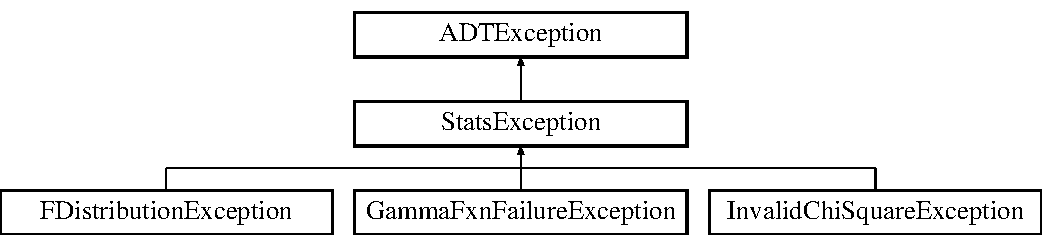
\includegraphics[height=3cm]{classStatsException}
\end{center}
\end{figure}


The documentation for this class was generated from the following file:\begin{DoxyCompactItemize}
\item 
engine/utils/\hyperlink{exceptions_8h}{exceptions.h}\end{DoxyCompactItemize}

\hypertarget{classStatsFillable}{
\section{StatsFillable Class Reference}
\label{classStatsFillable}\index{StatsFillable@{StatsFillable}}
}


{\ttfamily \#include $<$lr.hh$>$}

Inheritance diagram for StatsFillable:\begin{figure}[H]
\begin{center}
\leavevmode
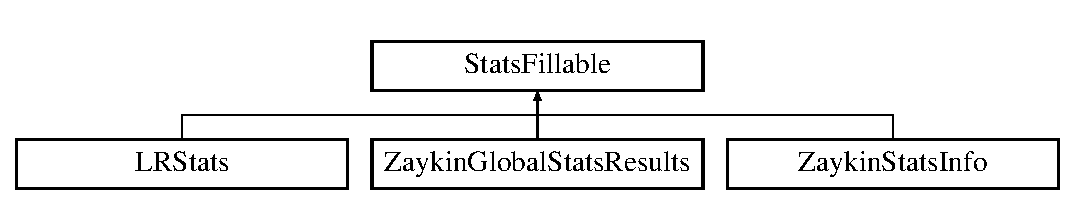
\includegraphics[height=2cm]{classStatsFillable}
\end{center}
\end{figure}
\subsection*{Public Member Functions}
\begin{DoxyCompactItemize}
\item 
virtual void \hyperlink{classStatsFillable_a6bc1a66ea949a078faa1b9ccdac54aba}{fillDefault} ()=0
\item 
virtual \hyperlink{classStatsFillable_a0a63c1e4b93f2614cb4b52bfd0b5c37c}{$\sim$StatsFillable} ()
\end{DoxyCompactItemize}


\subsection{Constructor \& Destructor Documentation}
\hypertarget{classStatsFillable_a0a63c1e4b93f2614cb4b52bfd0b5c37c}{
\index{StatsFillable@{StatsFillable}!$\sim$StatsFillable@{$\sim$StatsFillable}}
\index{$\sim$StatsFillable@{$\sim$StatsFillable}!StatsFillable@{StatsFillable}}
\subsubsection[{$\sim$StatsFillable}]{\setlength{\rightskip}{0pt plus 5cm}virtual StatsFillable::$\sim$StatsFillable ()\hspace{0.3cm}{\ttfamily  \mbox{[}inline, virtual\mbox{]}}}}
\label{classStatsFillable_a0a63c1e4b93f2614cb4b52bfd0b5c37c}


\subsection{Member Function Documentation}
\hypertarget{classStatsFillable_a6bc1a66ea949a078faa1b9ccdac54aba}{
\index{StatsFillable@{StatsFillable}!fillDefault@{fillDefault}}
\index{fillDefault@{fillDefault}!StatsFillable@{StatsFillable}}
\subsubsection[{fillDefault}]{\setlength{\rightskip}{0pt plus 5cm}virtual void StatsFillable::fillDefault ()\hspace{0.3cm}{\ttfamily  \mbox{[}pure virtual\mbox{]}}}}
\label{classStatsFillable_a6bc1a66ea949a078faa1b9ccdac54aba}


Implemented in \hyperlink{classLRStats_a42f08be70d011bef6da77f20ffc999fe}{LRStats}, \hyperlink{classZaykinStatsInfo_ac10ab8cf255d518161ce459ebcfdc8a4}{ZaykinStatsInfo}, and \hyperlink{classZaykinGlobalStatsResults_a6b45b4b6ad25c29a63363651345f0dbe}{ZaykinGlobalStatsResults}.



The documentation for this class was generated from the following file:\begin{DoxyCompactItemize}
\item 
engine/utils/\hyperlink{lr_8hh}{lr.hh}\end{DoxyCompactItemize}

\hypertarget{classZaykin}{
\section{Zaykin Class Reference}
\label{classZaykin}\index{Zaykin@{Zaykin}}
}


{\ttfamily \#include $<$zaykin.hh$>$}

\subsection*{Public Member Functions}
\begin{DoxyCompactItemize}
\item 
\hyperlink{classZaykin_a63cb6e8305dab0de45215665b45259a3}{Zaykin} ()
\item 
\hyperlink{classZaykin_a29f455c179a9dddc260fc6a580be2611}{$\sim$Zaykin} ()
\item 
void \hyperlink{classZaykin_a8f1f7c88b1f685b6d76b221e5fabe1d5}{setup} (const vector$<$ \hyperlink{structEMPersonalProbsResults}{EMPersonalProbsResults} $>$ \&, int numHaps, bool reweight)
\item 
\hyperlink{classZaykinGlobalStatsResults}{ZaykinGlobalStatsResults} \hyperlink{classZaykin_a61d28f9390301515bd9a47f8e6d631fb}{runGlobal} ()
\item 
vector$<$ double $>$ \hyperlink{classZaykin_a5afe5c8d000df0e1dce66d4a22891623}{runAllIndiv} (vector$<$ double $>$ \&testStats, vector$<$ int $>$ \&degsFreedom)
\item 
vector$<$ \hyperlink{classZaykinStatsInfo}{ZaykinStatsInfo} $>$ \hyperlink{classZaykin_af949cdfef60f62921b1128017c2dcc1d}{runAllHaplotypes} ()
\item 
void \hyperlink{classZaykin_afaa2e550bb5c905c428efc59dcef97f1}{setPhenotype} (const vector$<$ double $>$ \&p, const vector$<$ vector$<$ double $>$ $>$ \&c)
\item 
void \hyperlink{classZaykin_a61bed374552233240a4cd9e6df612976}{setKeepThresh} (int k)
\item 
void \hyperlink{classZaykin_a4bc760635a1333aedbc911244d543dc6}{setErrorInformation} (int \hyperlink{classZaykin_a03181d0afbfb93c0206e5c679561cafb}{snp}, int \hyperlink{classZaykin_ad0b5f025c5cffe4ef14f1685e956faa5}{numCovariates}, \hyperlink{classDataAccess}{DataAccess} $\ast$\hyperlink{classZaykin_a08bb927fb1ddebabaa02cfc3fe3c21b2}{data})
\end{DoxyCompactItemize}
\subsection*{Static Public Member Functions}
\begin{DoxyCompactItemize}
\item 
static int \hyperlink{classZaykin_ac26fd52252bbba304828e69e44d0a909}{test} ()
\end{DoxyCompactItemize}
\subsection*{Protected Member Functions}
\begin{DoxyCompactItemize}
\item 
int \hyperlink{classZaykin_aaaee27a7e56db508adf3f2c9bb9229d4}{recode12\_\-01} (int i)
\item 
void \hyperlink{classZaykin_a3a3b137409b8c862a66c70ce199721f6}{dump} (vector$<$ vector$<$ double $>$ $>$ m)
\item 
void \hyperlink{classZaykin_a769d85be4c6a2e177db4ae826259b5a1}{prepHaplotypes} (vector$<$ double $>$ \&ones, vector$<$ vector$<$ double $>$ $>$ \&haps)
\item 
\hyperlink{classZaykinStatsInfo}{ZaykinStatsInfo} \hyperlink{classZaykin_a48c7abad236fd142ec7da0e17da86356}{runLikelihoodRatio} (const vector$<$ double $>$ \&haps, const vector$<$ double $>$ \&ones)
\item 
void \hyperlink{classZaykin_aca4c79d7edc3bf5a62c73eb95d0ffb28}{handleException} (\hyperlink{classStatsFillable}{StatsFillable} \&stats, double \&startVal, int \&retry, const string \&message)
\end{DoxyCompactItemize}
\subsection*{Protected Attributes}
\begin{DoxyCompactItemize}
\item 
vector$<$ double $>$ \hyperlink{classZaykin_a19b6fa76c263b5eb7793957770bd4e22}{phenotype}
\item 
vector$<$ vector$<$ double $>$ $>$ \hyperlink{classZaykin_a7ab5edcff9494a41aef72ce33926bcb4}{cov}
\item 
vector$<$ vector$<$ double $>$ $>$ \hyperlink{classZaykin_ad86108c46b3feda98fd722146df86cec}{matrix}
\item 
vector$<$ bool $>$ \hyperlink{classZaykin_a7f47e07456e480212833d09b732be913}{usedHaplotype}
\item 
int \hyperlink{classZaykin_aae179a8aaed20ab73b219763a8bd8495}{keepThresh}
\item 
int \hyperlink{classZaykin_a03181d0afbfb93c0206e5c679561cafb}{snp}
\item 
int \hyperlink{classZaykin_ad0b5f025c5cffe4ef14f1685e956faa5}{numCovariates}
\item 
\hyperlink{classDataAccess}{DataAccess} $\ast$ \hyperlink{classZaykin_a08bb927fb1ddebabaa02cfc3fe3c21b2}{data}
\end{DoxyCompactItemize}
\subsection*{Friends}
\begin{DoxyCompactItemize}
\item 
class \hyperlink{classZaykin_ab5eb8e85b324a9728c593bdc1ada8198}{HaploStats}
\end{DoxyCompactItemize}


\subsection{Detailed Description}
Computation engine for Zaykin's method for haplo-\/genotype analysis.

Performs dom, add, rec tests per haplotype. Performs global test.

Requires that a phenotype and covariates be entered. Will cull haplotypes with global freq $<$ 0.05 and will either reweight the rest or keep the same depending on user flags.

\begin{DoxyAuthor}{Author}
Richard T. Guy 
\end{DoxyAuthor}


\subsection{Constructor \& Destructor Documentation}
\hypertarget{classZaykin_a63cb6e8305dab0de45215665b45259a3}{
\index{Zaykin@{Zaykin}!Zaykin@{Zaykin}}
\index{Zaykin@{Zaykin}!Zaykin@{Zaykin}}
\subsubsection[{Zaykin}]{\setlength{\rightskip}{0pt plus 5cm}Zaykin::Zaykin ()}}
\label{classZaykin_a63cb6e8305dab0de45215665b45259a3}
\hypertarget{classZaykin_a29f455c179a9dddc260fc6a580be2611}{
\index{Zaykin@{Zaykin}!$\sim$Zaykin@{$\sim$Zaykin}}
\index{$\sim$Zaykin@{$\sim$Zaykin}!Zaykin@{Zaykin}}
\subsubsection[{$\sim$Zaykin}]{\setlength{\rightskip}{0pt plus 5cm}Zaykin::$\sim$Zaykin ()}}
\label{classZaykin_a29f455c179a9dddc260fc6a580be2611}


\subsection{Member Function Documentation}
\hypertarget{classZaykin_a3a3b137409b8c862a66c70ce199721f6}{
\index{Zaykin@{Zaykin}!dump@{dump}}
\index{dump@{dump}!Zaykin@{Zaykin}}
\subsubsection[{dump}]{\setlength{\rightskip}{0pt plus 5cm}void Zaykin::dump (vector$<$ vector$<$ double $>$ $>$ {\em m})\hspace{0.3cm}{\ttfamily  \mbox{[}protected\mbox{]}}}}
\label{classZaykin_a3a3b137409b8c862a66c70ce199721f6}
Dump a vector to the screen for testing purposes only.


\begin{DoxyParams}{Parameters}
\item[{\em m}]A double vector to be printed. \end{DoxyParams}
\hypertarget{classZaykin_aca4c79d7edc3bf5a62c73eb95d0ffb28}{
\index{Zaykin@{Zaykin}!handleException@{handleException}}
\index{handleException@{handleException}!Zaykin@{Zaykin}}
\subsubsection[{handleException}]{\setlength{\rightskip}{0pt plus 5cm}void Zaykin::handleException ({\bf StatsFillable} \& {\em stats}, \/  double \& {\em startVal}, \/  int \& {\em retry}, \/  const string \& {\em message})\hspace{0.3cm}{\ttfamily  \mbox{[}protected\mbox{]}}}}
\label{classZaykin_aca4c79d7edc3bf5a62c73eb95d0ffb28}
\hypertarget{classZaykin_a769d85be4c6a2e177db4ae826259b5a1}{
\index{Zaykin@{Zaykin}!prepHaplotypes@{prepHaplotypes}}
\index{prepHaplotypes@{prepHaplotypes}!Zaykin@{Zaykin}}
\subsubsection[{prepHaplotypes}]{\setlength{\rightskip}{0pt plus 5cm}void Zaykin::prepHaplotypes (vector$<$ double $>$ \& {\em ones}, \/  vector$<$ vector$<$ double $>$ $>$ \& {\em haps})\hspace{0.3cm}{\ttfamily  \mbox{[}protected\mbox{]}}}}
\label{classZaykin_a769d85be4c6a2e177db4ae826259b5a1}
Prepare haplotypes. \hypertarget{classZaykin_aaaee27a7e56db508adf3f2c9bb9229d4}{
\index{Zaykin@{Zaykin}!recode12\_\-01@{recode12\_\-01}}
\index{recode12\_\-01@{recode12\_\-01}!Zaykin@{Zaykin}}
\subsubsection[{recode12\_\-01}]{\setlength{\rightskip}{0pt plus 5cm}int Zaykin::recode12\_\-01 (int {\em i})\hspace{0.3cm}{\ttfamily  \mbox{[}protected\mbox{]}}}}
\label{classZaykin_aaaee27a7e56db508adf3f2c9bb9229d4}
\hypertarget{classZaykin_af949cdfef60f62921b1128017c2dcc1d}{
\index{Zaykin@{Zaykin}!runAllHaplotypes@{runAllHaplotypes}}
\index{runAllHaplotypes@{runAllHaplotypes}!Zaykin@{Zaykin}}
\subsubsection[{runAllHaplotypes}]{\setlength{\rightskip}{0pt plus 5cm}vector$<$ {\bf ZaykinStatsInfo} $>$ Zaykin::runAllHaplotypes ()}}
\label{classZaykin_af949cdfef60f62921b1128017c2dcc1d}
Run each haplotype using Zaykin's method.

Assumes that usedHaplotype was set. \hypertarget{classZaykin_a5afe5c8d000df0e1dce66d4a22891623}{
\index{Zaykin@{Zaykin}!runAllIndiv@{runAllIndiv}}
\index{runAllIndiv@{runAllIndiv}!Zaykin@{Zaykin}}
\subsubsection[{runAllIndiv}]{\setlength{\rightskip}{0pt plus 5cm}vector$<$ double $>$ Zaykin::runAllIndiv (vector$<$ double $>$ \& {\em testStats}, \/  vector$<$ int $>$ \& {\em degsFreedom})}}
\label{classZaykin_a5afe5c8d000df0e1dce66d4a22891623}
Run all individual tests to test dom, add, rec relationship with each phenotype that had enough elements.

\begin{DoxyReturn}{Returns}
vector of pValues, one per person.
\end{DoxyReturn}
\begin{Desc}
\item[\hyperlink{bug__bug000003}{Bug}]This method not done yet. \end{Desc}
\hypertarget{classZaykin_a61d28f9390301515bd9a47f8e6d631fb}{
\index{Zaykin@{Zaykin}!runGlobal@{runGlobal}}
\index{runGlobal@{runGlobal}!Zaykin@{Zaykin}}
\subsubsection[{runGlobal}]{\setlength{\rightskip}{0pt plus 5cm}{\bf ZaykinGlobalStatsResults} Zaykin::runGlobal ()}}
\label{classZaykin_a61d28f9390301515bd9a47f8e6d631fb}
Run the global analysis. Put all data and covariates in a logistic regression model.

Compute likelihood ratio statistic. This uses a likelihood statistic where n-\/1 haplotypes are tested.

\begin{DoxyReturn}{Returns}
pvalue. 
\end{DoxyReturn}
\hypertarget{classZaykin_a48c7abad236fd142ec7da0e17da86356}{
\index{Zaykin@{Zaykin}!runLikelihoodRatio@{runLikelihoodRatio}}
\index{runLikelihoodRatio@{runLikelihoodRatio}!Zaykin@{Zaykin}}
\subsubsection[{runLikelihoodRatio}]{\setlength{\rightskip}{0pt plus 5cm}{\bf ZaykinStatsInfo} Zaykin::runLikelihoodRatio (const vector$<$ double $>$ \& {\em haps}, \/  const vector$<$ double $>$ \& {\em ones})\hspace{0.3cm}{\ttfamily  \mbox{[}protected\mbox{]}}}}
\label{classZaykin_a48c7abad236fd142ec7da0e17da86356}
Run a single likelihood ratio test. Assumes covariates and phenotype are set as global variables. The test is performed on the haps vector.


\begin{DoxyParams}{Parameters}
\item[{\em haps}]Haplotype variable. H\_\-0 is that this vector is independant. \item[{\em ones}]Set of ones. Precomputed for speed. \end{DoxyParams}
\begin{DoxyReturn}{Returns}
ZaykingStatsInfo should contain all information for this likelihood ratio test. 
\end{DoxyReturn}
\hypertarget{classZaykin_a4bc760635a1333aedbc911244d543dc6}{
\index{Zaykin@{Zaykin}!setErrorInformation@{setErrorInformation}}
\index{setErrorInformation@{setErrorInformation}!Zaykin@{Zaykin}}
\subsubsection[{setErrorInformation}]{\setlength{\rightskip}{0pt plus 5cm}void Zaykin::setErrorInformation (int {\em snp}, \/  int {\em numCovariates}, \/  {\bf DataAccess} $\ast$ {\em data})}}
\label{classZaykin_a4bc760635a1333aedbc911244d543dc6}
\hypertarget{classZaykin_a61bed374552233240a4cd9e6df612976}{
\index{Zaykin@{Zaykin}!setKeepThresh@{setKeepThresh}}
\index{setKeepThresh@{setKeepThresh}!Zaykin@{Zaykin}}
\subsubsection[{setKeepThresh}]{\setlength{\rightskip}{0pt plus 5cm}void Zaykin::setKeepThresh (int {\em k})\hspace{0.3cm}{\ttfamily  \mbox{[}inline\mbox{]}}}}
\label{classZaykin_a61bed374552233240a4cd9e6df612976}
Sets the keepThresh limit, which is min number of chromosomes that must contain a haplotype for it to be used in testing. 
\begin{DoxyParams}{Parameters}
\item[{\em k}]New threshold. \end{DoxyParams}
\hypertarget{classZaykin_afaa2e550bb5c905c428efc59dcef97f1}{
\index{Zaykin@{Zaykin}!setPhenotype@{setPhenotype}}
\index{setPhenotype@{setPhenotype}!Zaykin@{Zaykin}}
\subsubsection[{setPhenotype}]{\setlength{\rightskip}{0pt plus 5cm}void Zaykin::setPhenotype (const vector$<$ double $>$ \& {\em p}, \/  const vector$<$ vector$<$ double $>$ $>$ \& {\em c})}}
\label{classZaykin_afaa2e550bb5c905c428efc59dcef97f1}
\hypertarget{classZaykin_a8f1f7c88b1f685b6d76b221e5fabe1d5}{
\index{Zaykin@{Zaykin}!setup@{setup}}
\index{setup@{setup}!Zaykin@{Zaykin}}
\subsubsection[{setup}]{\setlength{\rightskip}{0pt plus 5cm}void Zaykin::setup (const vector$<$ {\bf EMPersonalProbsResults} $>$ \& {\em input}, \/  int {\em numHaps}, \/  bool {\em reweight})}}
\label{classZaykin_a8f1f7c88b1f685b6d76b221e5fabe1d5}
Retrieve data and build internal representation.

Given a series of haplogenotypes, for a given individual, calculate the prob of each haplotype involved.

The class variable matrix will be correctly filled with only those haplotypes that have greater than 0.05 global frequency. It will have been rescaled.

RTG updated Oct 14, 2010 to change the thresholding from 0.05\% global expression to showing up in at least n chromosomes (2m chr for m people). Default is 20.


\begin{DoxyParams}{Parameters}
\item[{\em input}]vector of \hyperlink{structEMPersonalProbsResults}{EMPersonalProbsResults} note that the person index is 0 based. \item[{\em numHaps}]total number of haplotypes. \item[{\em reweight}]If true, reweight the kept haplotypes. \end{DoxyParams}
\hypertarget{classZaykin_ac26fd52252bbba304828e69e44d0a909}{
\index{Zaykin@{Zaykin}!test@{test}}
\index{test@{test}!Zaykin@{Zaykin}}
\subsubsection[{test}]{\setlength{\rightskip}{0pt plus 5cm}int Zaykin::test ()\hspace{0.3cm}{\ttfamily  \mbox{[}static\mbox{]}}}}
\label{classZaykin_ac26fd52252bbba304828e69e44d0a909}


\subsection{Friends And Related Function Documentation}
\hypertarget{classZaykin_ab5eb8e85b324a9728c593bdc1ada8198}{
\index{Zaykin@{Zaykin}!HaploStats@{HaploStats}}
\index{HaploStats@{HaploStats}!Zaykin@{Zaykin}}
\subsubsection[{HaploStats}]{\setlength{\rightskip}{0pt plus 5cm}friend class {\bf HaploStats}\hspace{0.3cm}{\ttfamily  \mbox{[}friend\mbox{]}}}}
\label{classZaykin_ab5eb8e85b324a9728c593bdc1ada8198}


\subsection{Field Documentation}
\hypertarget{classZaykin_a7ab5edcff9494a41aef72ce33926bcb4}{
\index{Zaykin@{Zaykin}!cov@{cov}}
\index{cov@{cov}!Zaykin@{Zaykin}}
\subsubsection[{cov}]{\setlength{\rightskip}{0pt plus 5cm}vector$<$vector$<$double$>$ $>$ {\bf Zaykin::cov}\hspace{0.3cm}{\ttfamily  \mbox{[}protected\mbox{]}}}}
\label{classZaykin_a7ab5edcff9494a41aef72ce33926bcb4}
\hypertarget{classZaykin_a08bb927fb1ddebabaa02cfc3fe3c21b2}{
\index{Zaykin@{Zaykin}!data@{data}}
\index{data@{data}!Zaykin@{Zaykin}}
\subsubsection[{data}]{\setlength{\rightskip}{0pt plus 5cm}{\bf DataAccess}$\ast$ {\bf Zaykin::data}\hspace{0.3cm}{\ttfamily  \mbox{[}protected\mbox{]}}}}
\label{classZaykin_a08bb927fb1ddebabaa02cfc3fe3c21b2}
\hypertarget{classZaykin_aae179a8aaed20ab73b219763a8bd8495}{
\index{Zaykin@{Zaykin}!keepThresh@{keepThresh}}
\index{keepThresh@{keepThresh}!Zaykin@{Zaykin}}
\subsubsection[{keepThresh}]{\setlength{\rightskip}{0pt plus 5cm}int {\bf Zaykin::keepThresh}\hspace{0.3cm}{\ttfamily  \mbox{[}protected\mbox{]}}}}
\label{classZaykin_aae179a8aaed20ab73b219763a8bd8495}
\hypertarget{classZaykin_ad86108c46b3feda98fd722146df86cec}{
\index{Zaykin@{Zaykin}!matrix@{matrix}}
\index{matrix@{matrix}!Zaykin@{Zaykin}}
\subsubsection[{matrix}]{\setlength{\rightskip}{0pt plus 5cm}vector$<$vector$<$double$>$ $>$ {\bf Zaykin::matrix}\hspace{0.3cm}{\ttfamily  \mbox{[}protected\mbox{]}}}}
\label{classZaykin_ad86108c46b3feda98fd722146df86cec}
\hypertarget{classZaykin_ad0b5f025c5cffe4ef14f1685e956faa5}{
\index{Zaykin@{Zaykin}!numCovariates@{numCovariates}}
\index{numCovariates@{numCovariates}!Zaykin@{Zaykin}}
\subsubsection[{numCovariates}]{\setlength{\rightskip}{0pt plus 5cm}int {\bf Zaykin::numCovariates}\hspace{0.3cm}{\ttfamily  \mbox{[}protected\mbox{]}}}}
\label{classZaykin_ad0b5f025c5cffe4ef14f1685e956faa5}
\hypertarget{classZaykin_a19b6fa76c263b5eb7793957770bd4e22}{
\index{Zaykin@{Zaykin}!phenotype@{phenotype}}
\index{phenotype@{phenotype}!Zaykin@{Zaykin}}
\subsubsection[{phenotype}]{\setlength{\rightskip}{0pt plus 5cm}vector$<$double$>$ {\bf Zaykin::phenotype}\hspace{0.3cm}{\ttfamily  \mbox{[}protected\mbox{]}}}}
\label{classZaykin_a19b6fa76c263b5eb7793957770bd4e22}
\hypertarget{classZaykin_a03181d0afbfb93c0206e5c679561cafb}{
\index{Zaykin@{Zaykin}!snp@{snp}}
\index{snp@{snp}!Zaykin@{Zaykin}}
\subsubsection[{snp}]{\setlength{\rightskip}{0pt plus 5cm}int {\bf Zaykin::snp}\hspace{0.3cm}{\ttfamily  \mbox{[}protected\mbox{]}}}}
\label{classZaykin_a03181d0afbfb93c0206e5c679561cafb}
\hypertarget{classZaykin_a7f47e07456e480212833d09b732be913}{
\index{Zaykin@{Zaykin}!usedHaplotype@{usedHaplotype}}
\index{usedHaplotype@{usedHaplotype}!Zaykin@{Zaykin}}
\subsubsection[{usedHaplotype}]{\setlength{\rightskip}{0pt plus 5cm}vector$<$bool$>$ {\bf Zaykin::usedHaplotype}\hspace{0.3cm}{\ttfamily  \mbox{[}protected\mbox{]}}}}
\label{classZaykin_a7f47e07456e480212833d09b732be913}


The documentation for this class was generated from the following files:\begin{DoxyCompactItemize}
\item 
engine/utils/\hyperlink{zaykin_8hh}{zaykin.hh}\item 
engine/utils/\hyperlink{zaykin_8cpp}{zaykin.cpp}\end{DoxyCompactItemize}

\hypertarget{classZaykinGlobalStatsResults}{
\section{ZaykinGlobalStatsResults Class Reference}
\label{classZaykinGlobalStatsResults}\index{ZaykinGlobalStatsResults@{ZaykinGlobalStatsResults}}
}


{\ttfamily \#include $<$zaykin.hh$>$}

Inheritance diagram for ZaykinGlobalStatsResults:\begin{figure}[H]
\begin{center}
\leavevmode
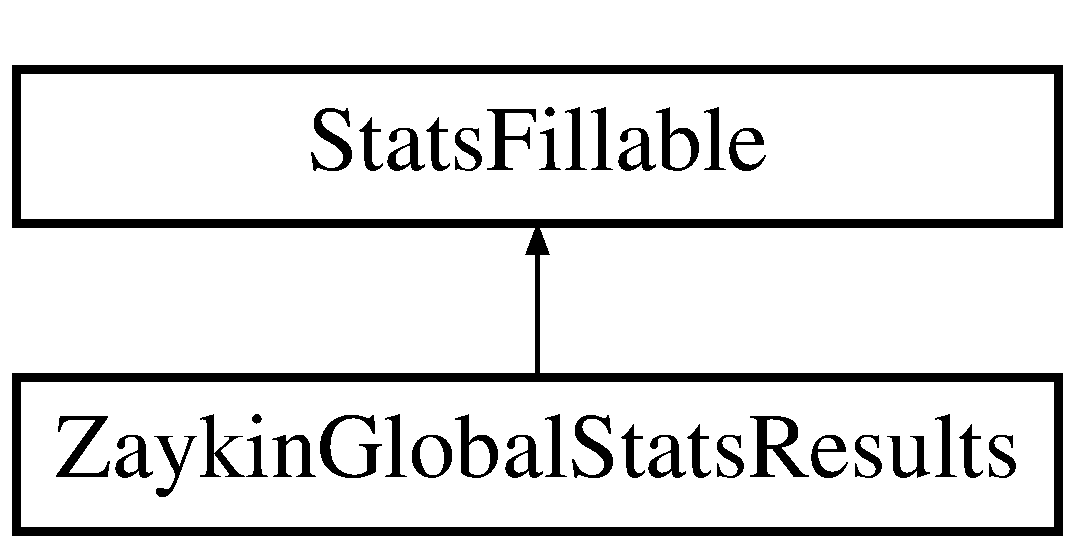
\includegraphics[height=2cm]{classZaykinGlobalStatsResults}
\end{center}
\end{figure}
\subsection*{Public Member Functions}
\begin{DoxyCompactItemize}
\item 
void \hyperlink{classZaykinGlobalStatsResults_a6b45b4b6ad25c29a63363651345f0dbe}{fillDefault} ()
\end{DoxyCompactItemize}
\subsection*{Data Fields}
\begin{DoxyCompactItemize}
\item 
int \hyperlink{classZaykinGlobalStatsResults_a4a9280a8dc6ea691eaadca1ae5438663}{degFreedom}
\item 
double \hyperlink{classZaykinGlobalStatsResults_aaedd2cf27b9e362ff177dd01a2809192}{testStat}
\item 
double \hyperlink{classZaykinGlobalStatsResults_ab8725b9e186651f5d41be92b4947152b}{pvalue}
\end{DoxyCompactItemize}


\subsection{Member Function Documentation}
\hypertarget{classZaykinGlobalStatsResults_a6b45b4b6ad25c29a63363651345f0dbe}{
\index{ZaykinGlobalStatsResults@{ZaykinGlobalStatsResults}!fillDefault@{fillDefault}}
\index{fillDefault@{fillDefault}!ZaykinGlobalStatsResults@{ZaykinGlobalStatsResults}}
\subsubsection[{fillDefault}]{\setlength{\rightskip}{0pt plus 5cm}void ZaykinGlobalStatsResults::fillDefault ()\hspace{0.3cm}{\ttfamily  \mbox{[}inline, virtual\mbox{]}}}}
\label{classZaykinGlobalStatsResults_a6b45b4b6ad25c29a63363651345f0dbe}


Implements \hyperlink{classStatsFillable_a6bc1a66ea949a078faa1b9ccdac54aba}{StatsFillable}.



\subsection{Field Documentation}
\hypertarget{classZaykinGlobalStatsResults_a4a9280a8dc6ea691eaadca1ae5438663}{
\index{ZaykinGlobalStatsResults@{ZaykinGlobalStatsResults}!degFreedom@{degFreedom}}
\index{degFreedom@{degFreedom}!ZaykinGlobalStatsResults@{ZaykinGlobalStatsResults}}
\subsubsection[{degFreedom}]{\setlength{\rightskip}{0pt plus 5cm}int {\bf ZaykinGlobalStatsResults::degFreedom}}}
\label{classZaykinGlobalStatsResults_a4a9280a8dc6ea691eaadca1ae5438663}
\hypertarget{classZaykinGlobalStatsResults_ab8725b9e186651f5d41be92b4947152b}{
\index{ZaykinGlobalStatsResults@{ZaykinGlobalStatsResults}!pvalue@{pvalue}}
\index{pvalue@{pvalue}!ZaykinGlobalStatsResults@{ZaykinGlobalStatsResults}}
\subsubsection[{pvalue}]{\setlength{\rightskip}{0pt plus 5cm}double {\bf ZaykinGlobalStatsResults::pvalue}}}
\label{classZaykinGlobalStatsResults_ab8725b9e186651f5d41be92b4947152b}
\hypertarget{classZaykinGlobalStatsResults_aaedd2cf27b9e362ff177dd01a2809192}{
\index{ZaykinGlobalStatsResults@{ZaykinGlobalStatsResults}!testStat@{testStat}}
\index{testStat@{testStat}!ZaykinGlobalStatsResults@{ZaykinGlobalStatsResults}}
\subsubsection[{testStat}]{\setlength{\rightskip}{0pt plus 5cm}double {\bf ZaykinGlobalStatsResults::testStat}}}
\label{classZaykinGlobalStatsResults_aaedd2cf27b9e362ff177dd01a2809192}


The documentation for this class was generated from the following file:\begin{DoxyCompactItemize}
\item 
engine/utils/\hyperlink{zaykin_8hh}{zaykin.hh}\end{DoxyCompactItemize}

\hypertarget{classZaykinStatsInfo}{
\section{ZaykinStatsInfo Class Reference}
\label{classZaykinStatsInfo}\index{ZaykinStatsInfo@{ZaykinStatsInfo}}
}


{\ttfamily \#include $<$zaykin.hh$>$}

Inheritance diagram for ZaykinStatsInfo:\begin{figure}[H]
\begin{center}
\leavevmode
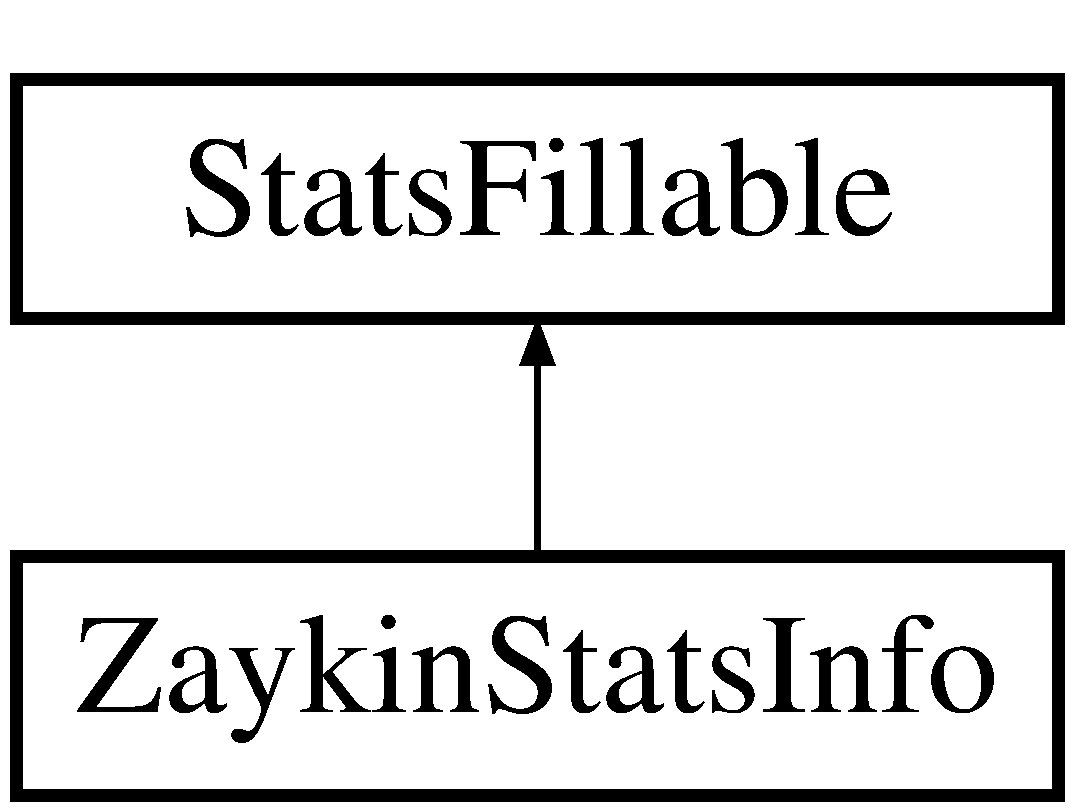
\includegraphics[height=2cm]{classZaykinStatsInfo}
\end{center}
\end{figure}
\subsection*{Public Member Functions}
\begin{DoxyCompactItemize}
\item 
void \hyperlink{classZaykinStatsInfo_ac10ab8cf255d518161ce459ebcfdc8a4}{fillDefault} ()
\end{DoxyCompactItemize}
\subsection*{Data Fields}
\begin{DoxyCompactItemize}
\item 
double \hyperlink{classZaykinStatsInfo_a28b66e969cdfd1f819ab622993aeea62}{chiSqStat}
\item 
int \hyperlink{classZaykinStatsInfo_aab543cdaa2227c8eda01598259bd0497}{degFree}
\item 
double \hyperlink{classZaykinStatsInfo_a75784cfcc143155568b6877fafe7c4a6}{OR}
\item 
double \hyperlink{classZaykinStatsInfo_a427af93fef8a99a23312fc42b14b85ae}{LCI}
\item 
double \hyperlink{classZaykinStatsInfo_ae32b8c048ddaddd014e5cb33943a3167}{UCI}
\end{DoxyCompactItemize}


\subsection{Detailed Description}
Holds information that is returned from a likelihood ratio test. 

\subsection{Member Function Documentation}
\hypertarget{classZaykinStatsInfo_ac10ab8cf255d518161ce459ebcfdc8a4}{
\index{ZaykinStatsInfo@{ZaykinStatsInfo}!fillDefault@{fillDefault}}
\index{fillDefault@{fillDefault}!ZaykinStatsInfo@{ZaykinStatsInfo}}
\subsubsection[{fillDefault}]{\setlength{\rightskip}{0pt plus 5cm}void ZaykinStatsInfo::fillDefault ()\hspace{0.3cm}{\ttfamily  \mbox{[}inline, virtual\mbox{]}}}}
\label{classZaykinStatsInfo_ac10ab8cf255d518161ce459ebcfdc8a4}


Implements \hyperlink{classStatsFillable_a6bc1a66ea949a078faa1b9ccdac54aba}{StatsFillable}.



\subsection{Field Documentation}
\hypertarget{classZaykinStatsInfo_a28b66e969cdfd1f819ab622993aeea62}{
\index{ZaykinStatsInfo@{ZaykinStatsInfo}!chiSqStat@{chiSqStat}}
\index{chiSqStat@{chiSqStat}!ZaykinStatsInfo@{ZaykinStatsInfo}}
\subsubsection[{chiSqStat}]{\setlength{\rightskip}{0pt plus 5cm}double {\bf ZaykinStatsInfo::chiSqStat}}}
\label{classZaykinStatsInfo_a28b66e969cdfd1f819ab622993aeea62}
\hypertarget{classZaykinStatsInfo_aab543cdaa2227c8eda01598259bd0497}{
\index{ZaykinStatsInfo@{ZaykinStatsInfo}!degFree@{degFree}}
\index{degFree@{degFree}!ZaykinStatsInfo@{ZaykinStatsInfo}}
\subsubsection[{degFree}]{\setlength{\rightskip}{0pt plus 5cm}int {\bf ZaykinStatsInfo::degFree}}}
\label{classZaykinStatsInfo_aab543cdaa2227c8eda01598259bd0497}
\hypertarget{classZaykinStatsInfo_a427af93fef8a99a23312fc42b14b85ae}{
\index{ZaykinStatsInfo@{ZaykinStatsInfo}!LCI@{LCI}}
\index{LCI@{LCI}!ZaykinStatsInfo@{ZaykinStatsInfo}}
\subsubsection[{LCI}]{\setlength{\rightskip}{0pt plus 5cm}double {\bf ZaykinStatsInfo::LCI}}}
\label{classZaykinStatsInfo_a427af93fef8a99a23312fc42b14b85ae}
\hypertarget{classZaykinStatsInfo_a75784cfcc143155568b6877fafe7c4a6}{
\index{ZaykinStatsInfo@{ZaykinStatsInfo}!OR@{OR}}
\index{OR@{OR}!ZaykinStatsInfo@{ZaykinStatsInfo}}
\subsubsection[{OR}]{\setlength{\rightskip}{0pt plus 5cm}double {\bf ZaykinStatsInfo::OR}}}
\label{classZaykinStatsInfo_a75784cfcc143155568b6877fafe7c4a6}
\hypertarget{classZaykinStatsInfo_ae32b8c048ddaddd014e5cb33943a3167}{
\index{ZaykinStatsInfo@{ZaykinStatsInfo}!UCI@{UCI}}
\index{UCI@{UCI}!ZaykinStatsInfo@{ZaykinStatsInfo}}
\subsubsection[{UCI}]{\setlength{\rightskip}{0pt plus 5cm}double {\bf ZaykinStatsInfo::UCI}}}
\label{classZaykinStatsInfo_ae32b8c048ddaddd014e5cb33943a3167}


The documentation for this class was generated from the following file:\begin{DoxyCompactItemize}
\item 
engine/utils/\hyperlink{zaykin_8hh}{zaykin.hh}\end{DoxyCompactItemize}

\chapter{File Documentation}
\hypertarget{ad__rule_8cpp}{
\section{engine/adtree/ad\_\-rule.cpp File Reference}
\label{ad__rule_8cpp}\index{engine/adtree/ad\_\-rule.cpp@{engine/adtree/ad\_\-rule.cpp}}
}
{\ttfamily \#include \char`\"{}ad\_\-rule.h\char`\"{}}\par
{\ttfamily \#include $<$string$>$}\par
{\ttfamily \#include $<$iostream$>$}\par
{\ttfamily \#include $<$sstream$>$}\par
{\ttfamily \#include $<$vector$>$}\par
{\ttfamily \#include \char`\"{}snp\_\-data.hh\char`\"{}}\par
{\ttfamily \#include \char`\"{}condition.h\char`\"{}}\par

\hypertarget{ad__rule_8h}{
\section{engine/adtree/ad\_\-rule.h File Reference}
\label{ad__rule_8h}\index{engine/adtree/ad\_\-rule.h@{engine/adtree/ad\_\-rule.h}}
}
{\ttfamily \#include $<$string$>$}\par
{\ttfamily \#include $<$iostream$>$}\par
{\ttfamily \#include $<$sstream$>$}\par
{\ttfamily \#include $<$vector$>$}\par
{\ttfamily \#include \char`\"{}condition.h\char`\"{}}\par
{\ttfamily \#include \char`\"{}precondition.h\char`\"{}}\par
\subsection*{Data Structures}
\begin{DoxyCompactItemize}
\item 
class \hyperlink{classAD__Rule}{AD\_\-Rule}
\end{DoxyCompactItemize}

\hypertarget{ad__tree__data_8cpp}{
\section{engine/adtree/ad\_\-tree\_\-data.cpp File Reference}
\label{ad__tree__data_8cpp}\index{engine/adtree/ad\_\-tree\_\-data.cpp@{engine/adtree/ad\_\-tree\_\-data.cpp}}
}
{\ttfamily \#include \char`\"{}ad\_\-tree\_\-data.h\char`\"{}}\par
{\ttfamily \#include \char`\"{}ad\_\-rule.h\char`\"{}}\par
{\ttfamily \#include \char`\"{}precondition.h\char`\"{}}\par
{\ttfamily \#include $<$map$>$}\par
{\ttfamily \#include $<$stdlib.h$>$}\par
{\ttfamily \#include $<$algorithm$>$}\par

\hypertarget{ad__tree__data_8h}{
\section{engine/adtree/ad\_\-tree\_\-data.h File Reference}
\label{ad__tree__data_8h}\index{engine/adtree/ad\_\-tree\_\-data.h@{engine/adtree/ad\_\-tree\_\-data.h}}
}
{\ttfamily \#include \char`\"{}ad\_\-rule.h\char`\"{}}\par
{\ttfamily \#include \char`\"{}precondition.h\char`\"{}}\par
{\ttfamily \#include $<$map$>$}\par
{\ttfamily \#include $<$stdlib.h$>$}\par
{\ttfamily \#include $<$algorithm$>$}\par
\subsection*{Data Structures}
\begin{DoxyCompactItemize}
\item 
class \hyperlink{classAD__Data}{AD\_\-Data}
\end{DoxyCompactItemize}

\hypertarget{adtree_8cpp}{
\section{engine/adtree/adtree.cpp File Reference}
\label{adtree_8cpp}\index{engine/adtree/adtree.cpp@{engine/adtree/adtree.cpp}}
}
{\ttfamily \#include \char`\"{}adtree.h\char`\"{}}\par
{\ttfamily \#include \char`\"{}snp\_\-data.hh\char`\"{}}\par
{\ttfamily \#include \char`\"{}engine.h\char`\"{}}\par
{\ttfamily \#include \char`\"{}ad\_\-rule.h\char`\"{}}\par
{\ttfamily \#include \char`\"{}ad\_\-tree\_\-data.h\char`\"{}}\par
{\ttfamily \#include $<$string$>$}\par
{\ttfamily \#include $<$fstream$>$}\par
{\ttfamily \#include $<$iostream$>$}\par
{\ttfamily \#include $<$stdlib.h$>$}\par
{\ttfamily \#include $<$vector$>$}\par
{\ttfamily \#include \char`\"{}param\_\-reader.h\char`\"{}}\par
{\ttfamily \#include $<$limits.h$>$}\par

\hypertarget{adtree_8h}{
\section{engine/adtree/adtree.h File Reference}
\label{adtree_8h}\index{engine/adtree/adtree.h@{engine/adtree/adtree.h}}
}
{\ttfamily \#include \char`\"{}../combinable.h\char`\"{}}\par
{\ttfamily \#include \char`\"{}ad\_\-rule.h\char`\"{}}\par
{\ttfamily \#include \char`\"{}ad\_\-tree\_\-data.h\char`\"{}}\par
{\ttfamily \#include \char`\"{}../../param/engine\_\-param\_\-reader.h\char`\"{}}\par
{\ttfamily \#include $<$limits.h$>$}\par
\subsection*{Data Structures}
\begin{DoxyCompactItemize}
\item 
class \hyperlink{classADTree}{ADTree}
\end{DoxyCompactItemize}

\hypertarget{condition_8cpp}{
\section{engine/adtree/condition.cpp File Reference}
\label{condition_8cpp}\index{engine/adtree/condition.cpp@{engine/adtree/condition.cpp}}
}
{\ttfamily \#include \char`\"{}condition.h\char`\"{}}\par

\hypertarget{condition_8h}{
\section{engine/adtree/condition.h File Reference}
\label{condition_8h}\index{engine/adtree/condition.h@{engine/adtree/condition.h}}
}
{\ttfamily \#include \char`\"{}../data\_\-plugin.h\char`\"{}}\par
{\ttfamily \#include $<$string$>$}\par
{\ttfamily \#include $<$vector$>$}\par
{\ttfamily \#include $<$sstream$>$}\par
\subsection*{Data Structures}
\begin{DoxyCompactItemize}
\item 
class \hyperlink{classCondition}{Condition}
\end{DoxyCompactItemize}

\hypertarget{precondition_8cpp}{
\section{engine/adtree/precondition.cpp File Reference}
\label{precondition_8cpp}\index{engine/adtree/precondition.cpp@{engine/adtree/precondition.cpp}}
}
{\ttfamily \#include \char`\"{}precondition.h\char`\"{}}\par

\hypertarget{precondition_8h}{
\section{engine/adtree/precondition.h File Reference}
\label{precondition_8h}\index{engine/adtree/precondition.h@{engine/adtree/precondition.h}}
}
{\ttfamily \#include \char`\"{}condition.h\char`\"{}}\par
{\ttfamily \#include $<$vector$>$}\par
\subsection*{Data Structures}
\begin{DoxyCompactItemize}
\item 
class \hyperlink{classPrecondition}{Precondition}
\end{DoxyCompactItemize}

\hypertarget{bagging_8cpp}{
\section{engine/bagging/bagging.cpp File Reference}
\label{bagging_8cpp}\index{engine/bagging/bagging.cpp@{engine/bagging/bagging.cpp}}
}
{\ttfamily \#include \char`\"{}bagging.h\char`\"{}}\par
{\ttfamily \#include \char`\"{}../combinable.h\char`\"{}}\par
{\ttfamily \#include \char`\"{}../adtree/adtree.h\char`\"{}}\par
{\ttfamily \#include \char`\"{}../../param/engine\_\-param\_\-reader.h\char`\"{}}\par
{\ttfamily \#include $<$string$>$}\par
{\ttfamily \#include $<$fstream$>$}\par
{\ttfamily \#include $<$iostream$>$}\par
{\ttfamily \#include $<$stdlib.h$>$}\par
{\ttfamily \#include $<$vector$>$}\par
{\ttfamily \#include $<$limits.h$>$}\par
{\ttfamily \#include $<$sstream$>$}\par

\hypertarget{bagging_8h}{
\section{engine/bagging/bagging.h File Reference}
\label{bagging_8h}\index{engine/bagging/bagging.h@{engine/bagging/bagging.h}}
}
{\ttfamily \#include \char`\"{}../combinable.h\char`\"{}}\par
{\ttfamily \#include \char`\"{}../adtree/adtree.h\char`\"{}}\par
{\ttfamily \#include \char`\"{}../../param/engine\_\-param\_\-reader.h\char`\"{}}\par
{\ttfamily \#include \char`\"{}../../param/param\_\-reader.h\char`\"{}}\par
{\ttfamily \#include $<$fstream$>$}\par
\subsection*{Data Structures}
\begin{DoxyCompactItemize}
\item 
class \hyperlink{classBagging}{Bagging}
\end{DoxyCompactItemize}

\hypertarget{combinable_8h}{
\section{engine/combinable.h File Reference}
\label{combinable_8h}\index{engine/combinable.h@{engine/combinable.h}}
}
{\ttfamily \#include \char`\"{}snp\_\-data.hh\char`\"{}}\par
{\ttfamily \#include $<$stdlib.h$>$}\par
{\ttfamily \#include $<$iostream$>$}\par
{\ttfamily \#include $<$sstream$>$}\par
{\ttfamily \#include $<$string$>$}\par
{\ttfamily \#include $<$vector$>$}\par
{\ttfamily \#include $<$map$>$}\par
{\ttfamily \#include $<$algorithm$>$}\par
{\ttfamily \#include \char`\"{}../param/param\_\-reader.h\char`\"{}}\par
{\ttfamily \#include $<$fstream$>$}\par
{\ttfamily \#include \char`\"{}../param/engine\_\-param\_\-reader.h\char`\"{}}\par
{\ttfamily \#include \char`\"{}../engine/snp\_\-data.hh\char`\"{}}\par
{\ttfamily \#include $<$ctype.h$>$}\par
{\ttfamily \#include $<$limits$>$}\par
{\ttfamily \#include \char`\"{}reader.h\char`\"{}}\par
{\ttfamily \#include \char`\"{}data\_\-plugin.h\char`\"{}}\par
{\ttfamily \#include $<$math.h$>$}\par
\subsection*{Data Structures}
\begin{DoxyCompactItemize}
\item 
class \hyperlink{classClassifies}{Classifies}
\end{DoxyCompactItemize}

\hypertarget{cross__val_8cpp}{
\section{engine/crossval/cross\_\-val.cpp File Reference}
\label{cross__val_8cpp}\index{engine/crossval/cross\_\-val.cpp@{engine/crossval/cross\_\-val.cpp}}
}
{\ttfamily \#include \char`\"{}cross\_\-val.h\char`\"{}}\par
{\ttfamily \#include \char`\"{}../engine.h\char`\"{}}\par
{\ttfamily \#include \char`\"{}../adtree/adtree.h\char`\"{}}\par
{\ttfamily \#include \char`\"{}../bagging/bagging.h\char`\"{}}\par
{\ttfamily \#include \char`\"{}../../param/param\_\-reader.h\char`\"{}}\par
{\ttfamily \#include $<$fstream$>$}\par

\hypertarget{cross__val_8h}{
\section{engine/crossval/cross\_\-val.h File Reference}
\label{cross__val_8h}\index{engine/crossval/cross\_\-val.h@{engine/crossval/cross\_\-val.h}}
}
{\ttfamily \#include \char`\"{}../engine.h\char`\"{}}\par
{\ttfamily \#include \char`\"{}../adtree/adtree.h\char`\"{}}\par
{\ttfamily \#include \char`\"{}../bagging/bagging.h\char`\"{}}\par
{\ttfamily \#include \char`\"{}../../param/param\_\-reader.h\char`\"{}}\par
{\ttfamily \#include $<$fstream$>$}\par
\subsection*{Data Structures}
\begin{DoxyCompactItemize}
\item 
class \hyperlink{classCrossValidation}{CrossValidation}
\end{DoxyCompactItemize}

\hypertarget{dandelion_8cpp}{
\section{engine/dandelion/dandelion.cpp File Reference}
\label{dandelion_8cpp}\index{engine/dandelion/dandelion.cpp@{engine/dandelion/dandelion.cpp}}
}
{\ttfamily \#include \char`\"{}dandelion.hh\char`\"{}}\par
{\ttfamily \#include $<$stdlib.h$>$}\par
{\ttfamily \#include $<$iostream$>$}\par
{\ttfamily \#include $<$string$>$}\par
{\ttfamily \#include $<$vector$>$}\par
{\ttfamily \#include \char`\"{}../../param/engine\_\-param\_\-reader.h\char`\"{}}\par
{\ttfamily \#include \char`\"{}../engine.h\char`\"{}}\par
{\ttfamily \#include \char`\"{}../randwh.h\char`\"{}}\par
{\ttfamily \#include \char`\"{}exceptions.h\char`\"{}}\par
{\ttfamily \#include $<$math.h$>$}\par
{\ttfamily \#include \char`\"{}haplotype.h\char`\"{}}\par
{\ttfamily \#include \char`\"{}output.h\char`\"{}}\par
{\ttfamily \#include \char`\"{}../../param/param\_\-reader.h\char`\"{}}\par
{\ttfamily \#include $<$sstream$>$}\par
{\ttfamily \#include $<$map$>$}\par
{\ttfamily \#include \char`\"{}statistics.h\char`\"{}}\par
{\ttfamily \#include \char`\"{}../em/em.h\char`\"{}}\par
{\ttfamily \#include \char`\"{}vecops.hh\char`\"{}}\par
{\ttfamily \#include $<$fstream$>$}\par
{\ttfamily \#include \char`\"{}lr.hh\char`\"{}}\par
{\ttfamily \#include $<$algorithm$>$}\par
{\ttfamily \#include \char`\"{}../utils/stringutils.h\char`\"{}}\par

\hypertarget{dandelion_8hh}{
\section{engine/dandelion/dandelion.hh File Reference}
\label{dandelion_8hh}\index{engine/dandelion/dandelion.hh@{engine/dandelion/dandelion.hh}}
}
{\ttfamily \#include $<$stdlib.h$>$}\par
{\ttfamily \#include $<$iostream$>$}\par
{\ttfamily \#include $<$string$>$}\par
{\ttfamily \#include $<$vector$>$}\par
{\ttfamily \#include \char`\"{}../../param/engine\_\-param\_\-reader.h\char`\"{}}\par
{\ttfamily \#include \char`\"{}../engine.h\char`\"{}}\par
{\ttfamily \#include \char`\"{}../randwh.h\char`\"{}}\par
{\ttfamily \#include \char`\"{}../em/em.h\char`\"{}}\par
{\ttfamily \#include \char`\"{}../output/dandelion\_\-out.hh\char`\"{}}\par
{\ttfamily \#include \char`\"{}../utils/zaykin.hh\char`\"{}}\par
{\ttfamily \#include \char`\"{}../ld/ld.h\char`\"{}}\par
\subsection*{Data Structures}
\begin{DoxyCompactItemize}
\item 
class \hyperlink{classDandelion}{Dandelion}
\end{DoxyCompactItemize}

\hypertarget{data__plugin_8cpp}{
\section{engine/data\_\-plugin.cpp File Reference}
\label{data__plugin_8cpp}\index{engine/data\_\-plugin.cpp@{engine/data\_\-plugin.cpp}}
}
{\ttfamily \#include \char`\"{}data\_\-plugin.h\char`\"{}}\par

\hypertarget{data__plugin_8h}{
\section{engine/data\_\-plugin.h File Reference}
\label{data__plugin_8h}\index{engine/data\_\-plugin.h@{engine/data\_\-plugin.h}}
}
{\ttfamily \#include \char`\"{}snp\_\-data.hh\char`\"{}}\par
\subsection*{Data Structures}
\begin{DoxyCompactItemize}
\item 
class \hyperlink{classDataAccess}{DataAccess}
\end{DoxyCompactItemize}

\hypertarget{em_8cpp}{
\section{engine/em/em.cpp File Reference}
\label{em_8cpp}\index{engine/em/em.cpp@{engine/em/em.cpp}}
}
{\ttfamily \#include \char`\"{}em.h\char`\"{}}\par

\hypertarget{em_8h}{
\section{engine/em/em.h File Reference}
\label{em_8h}\index{engine/em/em.h@{engine/em/em.h}}
}
{\ttfamily \#include $<$vector$>$}\par
{\ttfamily \#include $<$stdlib.h$>$}\par
{\ttfamily \#include \char`\"{}../utils/statistics.h\char`\"{}}\par
{\ttfamily \#include \char`\"{}haplotype.h\char`\"{}}\par
{\ttfamily \#include $<$iomanip$>$}\par
{\ttfamily \#include \char`\"{}../utils/vecops.hh\char`\"{}}\par
\subsection*{Data Structures}
\begin{DoxyCompactItemize}
\item 
struct \hyperlink{structEMPersonalProbsResults}{EMPersonalProbsResults}
\item 
class \hyperlink{classEM}{EM}
\end{DoxyCompactItemize}
\subsection*{Defines}
\begin{DoxyCompactItemize}
\item 
\#define \hyperlink{em_8h_a2c1808baba9949c6f505f2061cc1af9b}{DBG\_\-EM}~0
\end{DoxyCompactItemize}


\subsection{Define Documentation}
\hypertarget{em_8h_a2c1808baba9949c6f505f2061cc1af9b}{
\index{em.h@{em.h}!DBG\_\-EM@{DBG\_\-EM}}
\index{DBG\_\-EM@{DBG\_\-EM}!em.h@{em.h}}
\subsubsection[{DBG\_\-EM}]{\setlength{\rightskip}{0pt plus 5cm}\#define DBG\_\-EM~0}}
\label{em_8h_a2c1808baba9949c6f505f2061cc1af9b}
Expectation maximization algorithm. 
\hypertarget{haplotype_8cpp}{
\section{engine/em/haplotype.cpp File Reference}
\label{haplotype_8cpp}\index{engine/em/haplotype.cpp@{engine/em/haplotype.cpp}}
}
{\ttfamily \#include \char`\"{}haplotype.h\char`\"{}}\par
{\ttfamily \#include $<$iostream$>$}\par
{\ttfamily \#include $<$iomanip$>$}\par
{\ttfamily \#include $<$fstream$>$}\par

\hypertarget{haplotype_8h}{
\section{engine/em/haplotype.h File Reference}
\label{haplotype_8h}\index{engine/em/haplotype.h@{engine/em/haplotype.h}}
}
{\ttfamily \#include $<$vector$>$}\par
{\ttfamily \#include $<$iomanip$>$}\par
\subsection*{Data Structures}
\begin{DoxyCompactItemize}
\item 
class \hyperlink{classhaplotype}{haplotype}
\item 
class \hyperlink{classhaplotype_1_1alleleNumOutsideRangeEx}{haplotype::alleleNumOutsideRangeEx}
\end{DoxyCompactItemize}

\hypertarget{engine_8h}{
\section{engine/engine.h File Reference}
\label{engine_8h}\index{engine/engine.h@{engine/engine.h}}
}
{\ttfamily \#include \char`\"{}../param/param\_\-reader.h\char`\"{}}\par
{\ttfamily \#include \char`\"{}../param/engine\_\-param\_\-reader.h\char`\"{}}\par
{\ttfamily \#include \char`\"{}../reader/reader.h\char`\"{}}\par
{\ttfamily \#include \char`\"{}../reader/linkage\_\-reader.h\char`\"{}}\par
{\ttfamily \#include \char`\"{}data\_\-plugin.h\char`\"{}}\par
{\ttfamily \#include $<$math.h$>$}\par
\subsection*{Data Structures}
\begin{DoxyCompactItemize}
\item 
class \hyperlink{classEngine}{Engine}
\end{DoxyCompactItemize}

\hypertarget{intertwolog_8cpp}{
\section{engine/intertwolog/intertwolog.cpp File Reference}
\label{intertwolog_8cpp}\index{engine/intertwolog/intertwolog.cpp@{engine/intertwolog/intertwolog.cpp}}
}
{\ttfamily \#include \char`\"{}intertwolog.hh\char`\"{}}\par
{\ttfamily \#include $<$stdlib.h$>$}\par
{\ttfamily \#include $<$iostream$>$}\par
{\ttfamily \#include $<$string$>$}\par
{\ttfamily \#include $<$vector$>$}\par
{\ttfamily \#include \char`\"{}../../param/engine\_\-param\_\-reader.h\char`\"{}}\par
{\ttfamily \#include \char`\"{}../engine.h\char`\"{}}\par
{\ttfamily \#include \char`\"{}output.h\char`\"{}}\par
{\ttfamily \#include \char`\"{}../../param/param\_\-reader.h\char`\"{}}\par
{\ttfamily \#include $<$sstream$>$}\par
{\ttfamily \#include \char`\"{}../utils/stringutils.h\char`\"{}}\par
{\ttfamily \#include \char`\"{}../../logger/log.hh\char`\"{}}\par
{\ttfamily \#include \char`\"{}../utils/exceptions.h\char`\"{}}\par
{\ttfamily \#include \char`\"{}../utils/statistics.h\char`\"{}}\par
{\ttfamily \#include \char`\"{}../utils/float\_\-ops.hh\char`\"{}}\par
{\ttfamily \#include \char`\"{}vecops.hh\char`\"{}}\par
{\ttfamily \#include \char`\"{}ap.h\char`\"{}}\par
{\ttfamily \#include \char`\"{}alglibinternal.h\char`\"{}}\par
{\ttfamily \#include \char`\"{}alglibmisc.h\char`\"{}}\par
{\ttfamily \#include \char`\"{}ialglib.h\char`\"{}}\par
{\ttfamily \#include $<$math.h$>$}\par

\hypertarget{intertwolog_8hh}{
\section{engine/intertwolog/intertwolog.hh File Reference}
\label{intertwolog_8hh}\index{engine/intertwolog/intertwolog.hh@{engine/intertwolog/intertwolog.hh}}
}
{\ttfamily \#include $<$stdlib.h$>$}\par
{\ttfamily \#include $<$iostream$>$}\par
{\ttfamily \#include $<$string$>$}\par
{\ttfamily \#include $<$vector$>$}\par
{\ttfamily \#include \char`\"{}../../param/engine\_\-param\_\-reader.h\char`\"{}}\par
{\ttfamily \#include \char`\"{}../engine.h\char`\"{}}\par
{\ttfamily \#include \char`\"{}../output/intertwolog\_\-out.hh\char`\"{}}\par
{\ttfamily \#include \char`\"{}../utils/lr.hh\char`\"{}}\par
{\ttfamily \#include \char`\"{}../../logger/log.hh\char`\"{}}\par
\subsection*{Data Structures}
\begin{DoxyCompactItemize}
\item 
class \hyperlink{classInterTwoLog}{InterTwoLog}
\end{DoxyCompactItemize}
\subsection*{Defines}
\begin{DoxyCompactItemize}
\item 
\#define \hyperlink{intertwolog_8hh_a1c4f16246cf6aeda894aa254f41ccee4}{INTERTWOLOG\_\-TESTLOOP}~0
\item 
\#define \hyperlink{intertwolog_8hh_a336c9bf74cfeaaa050b253599b678c10}{RUN\_\-IN\_\-PARALLEL\_\-INTER}~1
\item 
\#define \hyperlink{intertwolog_8hh_acdfd99a66717dca63b6b480516e141c1}{INTERTWOLOG\_\-TESTSTATS}~0
\item 
\#define \hyperlink{intertwolog_8hh_af8fa7582dfcbc23a5cc0ada82cecdeb9}{INTERTWOLOG\_\-DATAPEAK}~0
\end{DoxyCompactItemize}


\subsection{Define Documentation}
\hypertarget{intertwolog_8hh_af8fa7582dfcbc23a5cc0ada82cecdeb9}{
\index{intertwolog.hh@{intertwolog.hh}!INTERTWOLOG\_\-DATAPEAK@{INTERTWOLOG\_\-DATAPEAK}}
\index{INTERTWOLOG\_\-DATAPEAK@{INTERTWOLOG\_\-DATAPEAK}!intertwolog.hh@{intertwolog.hh}}
\subsubsection[{INTERTWOLOG\_\-DATAPEAK}]{\setlength{\rightskip}{0pt plus 5cm}\#define INTERTWOLOG\_\-DATAPEAK~0}}
\label{intertwolog_8hh_af8fa7582dfcbc23a5cc0ada82cecdeb9}
\hypertarget{intertwolog_8hh_a1c4f16246cf6aeda894aa254f41ccee4}{
\index{intertwolog.hh@{intertwolog.hh}!INTERTWOLOG\_\-TESTLOOP@{INTERTWOLOG\_\-TESTLOOP}}
\index{INTERTWOLOG\_\-TESTLOOP@{INTERTWOLOG\_\-TESTLOOP}!intertwolog.hh@{intertwolog.hh}}
\subsubsection[{INTERTWOLOG\_\-TESTLOOP}]{\setlength{\rightskip}{0pt plus 5cm}\#define INTERTWOLOG\_\-TESTLOOP~0}}
\label{intertwolog_8hh_a1c4f16246cf6aeda894aa254f41ccee4}
\hypertarget{intertwolog_8hh_acdfd99a66717dca63b6b480516e141c1}{
\index{intertwolog.hh@{intertwolog.hh}!INTERTWOLOG\_\-TESTSTATS@{INTERTWOLOG\_\-TESTSTATS}}
\index{INTERTWOLOG\_\-TESTSTATS@{INTERTWOLOG\_\-TESTSTATS}!intertwolog.hh@{intertwolog.hh}}
\subsubsection[{INTERTWOLOG\_\-TESTSTATS}]{\setlength{\rightskip}{0pt plus 5cm}\#define INTERTWOLOG\_\-TESTSTATS~0}}
\label{intertwolog_8hh_acdfd99a66717dca63b6b480516e141c1}
\hypertarget{intertwolog_8hh_a336c9bf74cfeaaa050b253599b678c10}{
\index{intertwolog.hh@{intertwolog.hh}!RUN\_\-IN\_\-PARALLEL\_\-INTER@{RUN\_\-IN\_\-PARALLEL\_\-INTER}}
\index{RUN\_\-IN\_\-PARALLEL\_\-INTER@{RUN\_\-IN\_\-PARALLEL\_\-INTER}!intertwolog.hh@{intertwolog.hh}}
\subsubsection[{RUN\_\-IN\_\-PARALLEL\_\-INTER}]{\setlength{\rightskip}{0pt plus 5cm}\#define RUN\_\-IN\_\-PARALLEL\_\-INTER~1}}
\label{intertwolog_8hh_a336c9bf74cfeaaa050b253599b678c10}

\hypertarget{ld_8cpp}{
\section{engine/ld/ld.cpp File Reference}
\label{ld_8cpp}\index{engine/ld/ld.cpp@{engine/ld/ld.cpp}}
}
{\ttfamily \#include \char`\"{}ld.h\char`\"{}}\par

\hypertarget{ld_8h}{
\section{engine/ld/ld.h File Reference}
\label{ld_8h}\index{engine/ld/ld.h@{engine/ld/ld.h}}
}
{\ttfamily \#include $<$stdlib.h$>$}\par
{\ttfamily \#include $<$iostream$>$}\par
{\ttfamily \#include $<$string$>$}\par
{\ttfamily \#include $<$vector$>$}\par
{\ttfamily \#include $<$algorithm$>$}\par
{\ttfamily \#include \char`\"{}../../param/engine\_\-param\_\-reader.h\char`\"{}}\par
{\ttfamily \#include \char`\"{}../engine.h\char`\"{}}\par
{\ttfamily \#include \char`\"{}../randwh.h\char`\"{}}\par
{\ttfamily \#include \char`\"{}../em/em.h\char`\"{}}\par
{\ttfamily \#include \char`\"{}../output/dprime\_\-out.h\char`\"{}}\par
\subsection*{Data Structures}
\begin{DoxyCompactItemize}
\item 
class \hyperlink{classLinkageDisequilibrium}{LinkageDisequilibrium}
\end{DoxyCompactItemize}
\subsection*{Defines}
\begin{DoxyCompactItemize}
\item 
\#define \hyperlink{ld_8h_aaa6e8ecdb1cab467e669c5fbdefffbd5}{RUN\_\-IN\_\-PARALLEL\_\-LD}~1
\end{DoxyCompactItemize}


\subsection{Define Documentation}
\hypertarget{ld_8h_aaa6e8ecdb1cab467e669c5fbdefffbd5}{
\index{ld.h@{ld.h}!RUN\_\-IN\_\-PARALLEL\_\-LD@{RUN\_\-IN\_\-PARALLEL\_\-LD}}
\index{RUN\_\-IN\_\-PARALLEL\_\-LD@{RUN\_\-IN\_\-PARALLEL\_\-LD}!ld.h@{ld.h}}
\subsubsection[{RUN\_\-IN\_\-PARALLEL\_\-LD}]{\setlength{\rightskip}{0pt plus 5cm}\#define RUN\_\-IN\_\-PARALLEL\_\-LD~1}}
\label{ld_8h_aaa6e8ecdb1cab467e669c5fbdefffbd5}

\hypertarget{dandelion__out_8cpp}{
\section{engine/output/dandelion\_\-out.cpp File Reference}
\label{dandelion__out_8cpp}\index{engine/output/dandelion\_\-out.cpp@{engine/output/dandelion\_\-out.cpp}}
}
{\ttfamily \#include \char`\"{}dandelion\_\-out.hh\char`\"{}}\par

\hypertarget{dandelion__out_8hh}{
\section{engine/output/dandelion\_\-out.hh File Reference}
\label{dandelion__out_8hh}\index{engine/output/dandelion\_\-out.hh@{engine/output/dandelion\_\-out.hh}}
}
{\ttfamily \#include \char`\"{}output.h\char`\"{}}\par
{\ttfamily \#include $<$iostream$>$}\par
{\ttfamily \#include $<$string$>$}\par
{\ttfamily \#include $<$map$>$}\par
{\ttfamily \#include $<$fstream$>$}\par
{\ttfamily \#include \char`\"{}../../param/param\_\-reader.h\char`\"{}}\par
{\ttfamily \#include \char`\"{}../../param/engine\_\-param\_\-reader.h\char`\"{}}\par
{\ttfamily \#include $<$sstream$>$}\par
{\ttfamily \#include \char`\"{}../utils/stringutils.h\char`\"{}}\par
\subsection*{Data Structures}
\begin{DoxyCompactItemize}
\item 
struct \hyperlink{structDandelionSnpInfo}{DandelionSnpInfo}
\item 
struct \hyperlink{structDandelionHaploInfo}{DandelionHaploInfo}
\item 
struct \hyperlink{structDandelionPProbInfo}{DandelionPProbInfo}
\item 
class \hyperlink{classDandelionOutput}{DandelionOutput}
\end{DoxyCompactItemize}

\hypertarget{dprime__out_8cpp}{
\section{engine/output/dprime\_\-out.cpp File Reference}
\label{dprime__out_8cpp}\index{engine/output/dprime\_\-out.cpp@{engine/output/dprime\_\-out.cpp}}
}
{\ttfamily \#include \char`\"{}dprime\_\-out.h\char`\"{}}\par

\hypertarget{dprime__out_8h}{
\section{engine/output/dprime\_\-out.h File Reference}
\label{dprime__out_8h}\index{engine/output/dprime\_\-out.h@{engine/output/dprime\_\-out.h}}
}
{\ttfamily \#include \char`\"{}output.h\char`\"{}}\par
{\ttfamily \#include \char`\"{}../../param/param\_\-reader.h\char`\"{}}\par
{\ttfamily \#include $<$sstream$>$}\par
{\ttfamily \#include $<$map$>$}\par
{\ttfamily \#include \char`\"{}../utils/stringutils.h\char`\"{}}\par
\subsection*{Data Structures}
\begin{DoxyCompactItemize}
\item 
struct \hyperlink{structLinkageMeasures}{LinkageMeasures}
\item 
class \hyperlink{classLinkageOutput}{LinkageOutput}
\end{DoxyCompactItemize}

\hypertarget{intertwolog__out_8cpp}{
\section{engine/output/intertwolog\_\-out.cpp File Reference}
\label{intertwolog__out_8cpp}\index{engine/output/intertwolog\_\-out.cpp@{engine/output/intertwolog\_\-out.cpp}}
}
{\ttfamily \#include \char`\"{}intertwolog\_\-out.hh\char`\"{}}\par

\hypertarget{intertwolog__out_8hh}{
\section{engine/output/intertwolog\_\-out.hh File Reference}
\label{intertwolog__out_8hh}\index{engine/output/intertwolog\_\-out.hh@{engine/output/intertwolog\_\-out.hh}}
}
{\ttfamily \#include \char`\"{}output.h\char`\"{}}\par
{\ttfamily \#include \char`\"{}../../param/param\_\-reader.h\char`\"{}}\par
{\ttfamily \#include \char`\"{}../../param/engine\_\-param\_\-reader.h\char`\"{}}\par
{\ttfamily \#include $<$sstream$>$}\par
{\ttfamily \#include \char`\"{}../utils/stringutils.h\char`\"{}}\par
{\ttfamily \#include \char`\"{}../../logger/log.hh\char`\"{}}\par
\subsection*{Data Structures}
\begin{DoxyCompactItemize}
\item 
struct \hyperlink{structInterTwoLogMeasures}{InterTwoLogMeasures}
\item 
class \hyperlink{classInterTwoLogOutput}{InterTwoLogOutput}
\end{DoxyCompactItemize}

\hypertarget{output_8cpp}{
\section{engine/output/output.cpp File Reference}
\label{output_8cpp}\index{engine/output/output.cpp@{engine/output/output.cpp}}
}
{\ttfamily \#include \char`\"{}output.h\char`\"{}}\par

\hypertarget{output_8h}{
\section{engine/output/output.h File Reference}
\label{output_8h}\index{engine/output/output.h@{engine/output/output.h}}
}
{\ttfamily \#include $<$iostream$>$}\par
{\ttfamily \#include $<$string$>$}\par
{\ttfamily \#include $<$map$>$}\par
{\ttfamily \#include $<$fstream$>$}\par
\subsection*{Data Structures}
\begin{DoxyCompactItemize}
\item 
class \hyperlink{classOutput}{Output}
\end{DoxyCompactItemize}

\hypertarget{qsnpgwa__out_8cpp}{
\section{engine/output/qsnpgwa\_\-out.cpp File Reference}
\label{qsnpgwa__out_8cpp}\index{engine/output/qsnpgwa\_\-out.cpp@{engine/output/qsnpgwa\_\-out.cpp}}
}
{\ttfamily \#include \char`\"{}qsnpgwa\_\-out.hh\char`\"{}}\par
{\ttfamily \#include \char`\"{}output.h\char`\"{}}\par
{\ttfamily \#include $<$string$>$}\par
{\ttfamily \#include \char`\"{}../utils/stringutils.h\char`\"{}}\par
{\ttfamily \#include $<$ostream$>$}\par
{\ttfamily \#include \char`\"{}../../param/param\_\-reader.h\char`\"{}}\par
{\ttfamily \#include \char`\"{}../../param/engine\_\-param\_\-reader.h\char`\"{}}\par
{\ttfamily \#include $<$sstream$>$}\par
{\ttfamily \#include $<$map$>$}\par

\hypertarget{qsnpgwa__out_8hh}{
\section{engine/output/qsnpgwa\_\-out.hh File Reference}
\label{qsnpgwa__out_8hh}\index{engine/output/qsnpgwa\_\-out.hh@{engine/output/qsnpgwa\_\-out.hh}}
}
{\ttfamily \#include \char`\"{}output.h\char`\"{}}\par
{\ttfamily \#include \char`\"{}snpinfo\_\-out.hh\char`\"{}}\par
{\ttfamily \#include \char`\"{}../../param/param\_\-reader.h\char`\"{}}\par
{\ttfamily \#include \char`\"{}../../param/engine\_\-param\_\-reader.h\char`\"{}}\par
{\ttfamily \#include $<$sstream$>$}\par
{\ttfamily \#include $<$map$>$}\par
{\ttfamily \#include \char`\"{}../utils/stringutils.h\char`\"{}}\par
\subsection*{Data Structures}
\begin{DoxyCompactItemize}
\item 
struct \hyperlink{structContPopStatsResults}{ContPopStatsResults}
\item 
struct \hyperlink{structContGenoStatsResults}{ContGenoStatsResults}
\item 
class \hyperlink{classQSnpgwaOutput}{QSnpgwaOutput}
\end{DoxyCompactItemize}

\hypertarget{snpgwa__out_8cpp}{
\section{engine/output/snpgwa\_\-out.cpp File Reference}
\label{snpgwa__out_8cpp}\index{engine/output/snpgwa\_\-out.cpp@{engine/output/snpgwa\_\-out.cpp}}
}
{\ttfamily \#include \char`\"{}snpgwa\_\-out.hh\char`\"{}}\par
{\ttfamily \#include \char`\"{}output.h\char`\"{}}\par
{\ttfamily \#include \char`\"{}snpinfo\_\-out.hh\char`\"{}}\par
{\ttfamily \#include \char`\"{}../../param/param\_\-reader.h\char`\"{}}\par
{\ttfamily \#include \char`\"{}../../param/engine\_\-param\_\-reader.h\char`\"{}}\par
{\ttfamily \#include $<$sstream$>$}\par
{\ttfamily \#include $<$map$>$}\par
{\ttfamily \#include \char`\"{}../utils/stringutils.h\char`\"{}}\par
{\ttfamily \#include \char`\"{}../../logger/log.hh\char`\"{}}\par
{\ttfamily \#include $<$time.h$>$}\par

\hypertarget{snpgwa__out_8hh}{
\section{engine/output/snpgwa\_\-out.hh File Reference}
\label{snpgwa__out_8hh}\index{engine/output/snpgwa\_\-out.hh@{engine/output/snpgwa\_\-out.hh}}
}
{\ttfamily \#include \char`\"{}output.h\char`\"{}}\par
{\ttfamily \#include \char`\"{}snpinfo\_\-out.hh\char`\"{}}\par
{\ttfamily \#include \char`\"{}../../param/param\_\-reader.h\char`\"{}}\par
{\ttfamily \#include \char`\"{}../../param/engine\_\-param\_\-reader.h\char`\"{}}\par
{\ttfamily \#include $<$sstream$>$}\par
{\ttfamily \#include $<$map$>$}\par
{\ttfamily \#include \char`\"{}../utils/stringutils.h\char`\"{}}\par
{\ttfamily \#include \char`\"{}../../logger/log.hh\char`\"{}}\par
{\ttfamily \#include $<$time.h$>$}\par
\subsection*{Data Structures}
\begin{DoxyCompactItemize}
\item 
struct \hyperlink{structPopStatsResults}{PopStatsResults}
\item 
struct \hyperlink{structGenoStatsResults}{GenoStatsResults}
\item 
struct \hyperlink{structHaploStatsResults}{HaploStatsResults}
\item 
class \hyperlink{classSnpgwaOutput}{SnpgwaOutput}
\end{DoxyCompactItemize}

\hypertarget{snpinfo__out_8cpp}{
\section{engine/output/snpinfo\_\-out.cpp File Reference}
\label{snpinfo__out_8cpp}\index{engine/output/snpinfo\_\-out.cpp@{engine/output/snpinfo\_\-out.cpp}}
}
{\ttfamily \#include \char`\"{}snpinfo\_\-out.hh\char`\"{}}\par

\hypertarget{snpinfo__out_8hh}{
\section{engine/output/snpinfo\_\-out.hh File Reference}
\label{snpinfo__out_8hh}\index{engine/output/snpinfo\_\-out.hh@{engine/output/snpinfo\_\-out.hh}}
}
{\ttfamily \#include $<$string$>$}\par
{\ttfamily \#include \char`\"{}../utils/stringutils.h\char`\"{}}\par
{\ttfamily \#include $<$ostream$>$}\par
\subsection*{Data Structures}
\begin{DoxyCompactItemize}
\item 
class \hyperlink{classSnpInfo}{SnpInfo}
\end{DoxyCompactItemize}

\hypertarget{cont__genostats_8cpp}{
\section{engine/qsnpgwa/cont\_\-genostats.cpp File Reference}
\label{cont__genostats_8cpp}\index{engine/qsnpgwa/cont\_\-genostats.cpp@{engine/qsnpgwa/cont\_\-genostats.cpp}}
}
{\ttfamily \#include \char`\"{}cont\_\-genostats.hh\char`\"{}}\par
{\ttfamily \#include \char`\"{}../engine.h\char`\"{}}\par
{\ttfamily \#include \char`\"{}../utils/statistics.h\char`\"{}}\par
{\ttfamily \#include \char`\"{}../output/qsnpgwa\_\-out.hh\char`\"{}}\par
{\ttfamily \#include \char`\"{}../utils/exceptions.h\char`\"{}}\par
{\ttfamily \#include \char`\"{}../utils/float\_\-ops.hh\char`\"{}}\par
{\ttfamily \#include \char`\"{}../libs/linalg.h\char`\"{}}\par
{\ttfamily \#include \char`\"{}../libs/alglibinternal.h\char`\"{}}\par
{\ttfamily \#include \char`\"{}../libs/blas.h\char`\"{}}\par
{\ttfamily \#include \char`\"{}../../logger/log.hh\char`\"{}}\par

\hypertarget{cont__genostats_8hh}{
\section{engine/qsnpgwa/cont\_\-genostats.hh File Reference}
\label{cont__genostats_8hh}\index{engine/qsnpgwa/cont\_\-genostats.hh@{engine/qsnpgwa/cont\_\-genostats.hh}}
}
{\ttfamily \#include \char`\"{}../engine.h\char`\"{}}\par
{\ttfamily \#include \char`\"{}../utils/statistics.h\char`\"{}}\par
{\ttfamily \#include \char`\"{}../output/qsnpgwa\_\-out.hh\char`\"{}}\par
{\ttfamily \#include \char`\"{}../utils/linear\_\-regression.hh\char`\"{}}\par
{\ttfamily \#include \char`\"{}../../logger/log.hh\char`\"{}}\par
\subsection*{Data Structures}
\begin{DoxyCompactItemize}
\item 
class \hyperlink{classContGenoStats}{ContGenoStats}
\item 
struct \hyperlink{structContGenoStats_1_1statisticsOutput}{ContGenoStats::statisticsOutput}
\end{DoxyCompactItemize}
\subsection*{Defines}
\begin{DoxyCompactItemize}
\item 
\#define \hyperlink{cont__genostats_8hh_a046156af077879b5287605a7dafcac9c}{CONT\_\-GENOSTATS\_\-STATS}~0
\end{DoxyCompactItemize}


\subsection{Define Documentation}
\hypertarget{cont__genostats_8hh_a046156af077879b5287605a7dafcac9c}{
\index{cont\_\-genostats.hh@{cont\_\-genostats.hh}!CONT\_\-GENOSTATS\_\-STATS@{CONT\_\-GENOSTATS\_\-STATS}}
\index{CONT\_\-GENOSTATS\_\-STATS@{CONT\_\-GENOSTATS\_\-STATS}!cont_genostats.hh@{cont\_\-genostats.hh}}
\subsubsection[{CONT\_\-GENOSTATS\_\-STATS}]{\setlength{\rightskip}{0pt plus 5cm}\#define CONT\_\-GENOSTATS\_\-STATS~0}}
\label{cont__genostats_8hh_a046156af077879b5287605a7dafcac9c}

\hypertarget{cont__popstats_8cpp}{
\section{engine/qsnpgwa/cont\_\-popstats.cpp File Reference}
\label{cont__popstats_8cpp}\index{engine/qsnpgwa/cont\_\-popstats.cpp@{engine/qsnpgwa/cont\_\-popstats.cpp}}
}
{\ttfamily \#include \char`\"{}cont\_\-popstats.hh\char`\"{}}\par
{\ttfamily \#include \char`\"{}../utils/exceptions.h\char`\"{}}\par
{\ttfamily \#include $<$deque$>$}\par
{\ttfamily \#include \char`\"{}../engine.h\char`\"{}}\par
{\ttfamily \#include \char`\"{}../utils/statistics.h\char`\"{}}\par
{\ttfamily \#include \char`\"{}../utils/vecops.hh\char`\"{}}\par
{\ttfamily \#include \char`\"{}../output/snpgwa\_\-out.hh\char`\"{}}\par
{\ttfamily \#include \char`\"{}../output/qsnpgwa\_\-out.hh\char`\"{}}\par

\hypertarget{cont__popstats_8hh}{
\section{engine/qsnpgwa/cont\_\-popstats.hh File Reference}
\label{cont__popstats_8hh}\index{engine/qsnpgwa/cont\_\-popstats.hh@{engine/qsnpgwa/cont\_\-popstats.hh}}
}
{\ttfamily \#include \char`\"{}../utils/exceptions.h\char`\"{}}\par
{\ttfamily \#include $<$deque$>$}\par
{\ttfamily \#include \char`\"{}../engine.h\char`\"{}}\par
{\ttfamily \#include \char`\"{}../utils/statistics.h\char`\"{}}\par
{\ttfamily \#include \char`\"{}../snpgwa/popstats.hh\char`\"{}}\par
{\ttfamily \#include \char`\"{}../output/qsnpgwa\_\-out.hh\char`\"{}}\par
\subsection*{Data Structures}
\begin{DoxyCompactItemize}
\item 
class \hyperlink{classContPopStats}{ContPopStats}
\end{DoxyCompactItemize}
\subsection*{Defines}
\begin{DoxyCompactItemize}
\item 
\#define \hyperlink{cont__popstats_8hh_a4125f6093c3e688a9d81f49afd282d45}{CONT\_\-POPSTATS\_\-H}
\end{DoxyCompactItemize}


\subsection{Define Documentation}
\hypertarget{cont__popstats_8hh_a4125f6093c3e688a9d81f49afd282d45}{
\index{cont\_\-popstats.hh@{cont\_\-popstats.hh}!CONT\_\-POPSTATS\_\-H@{CONT\_\-POPSTATS\_\-H}}
\index{CONT\_\-POPSTATS\_\-H@{CONT\_\-POPSTATS\_\-H}!cont_popstats.hh@{cont\_\-popstats.hh}}
\subsubsection[{CONT\_\-POPSTATS\_\-H}]{\setlength{\rightskip}{0pt plus 5cm}\#define CONT\_\-POPSTATS\_\-H}}
\label{cont__popstats_8hh_a4125f6093c3e688a9d81f49afd282d45}

\hypertarget{qsnpgwa_8cpp}{
\section{engine/qsnpgwa/qsnpgwa.cpp File Reference}
\label{qsnpgwa_8cpp}\index{engine/qsnpgwa/qsnpgwa.cpp@{engine/qsnpgwa/qsnpgwa.cpp}}
}
{\ttfamily \#include \char`\"{}qsnpgwa.hh\char`\"{}}\par
{\ttfamily \#include \char`\"{}../../param/engine\_\-param\_\-reader.h\char`\"{}}\par
{\ttfamily \#include \char`\"{}../engine.h\char`\"{}}\par
{\ttfamily \#include \char`\"{}../output/qsnpgwa\_\-out.hh\char`\"{}}\par
{\ttfamily \#include \char`\"{}cont\_\-popstats.hh\char`\"{}}\par
{\ttfamily \#include \char`\"{}cont\_\-genostats.hh\char`\"{}}\par
{\ttfamily \#include \char`\"{}../ld/ld.h\char`\"{}}\par

\hypertarget{qsnpgwa_8hh}{
\section{engine/qsnpgwa/qsnpgwa.hh File Reference}
\label{qsnpgwa_8hh}\index{engine/qsnpgwa/qsnpgwa.hh@{engine/qsnpgwa/qsnpgwa.hh}}
}
{\ttfamily \#include \char`\"{}../../param/engine\_\-param\_\-reader.h\char`\"{}}\par
{\ttfamily \#include \char`\"{}../engine.h\char`\"{}}\par
{\ttfamily \#include \char`\"{}../output/qsnpgwa\_\-out.hh\char`\"{}}\par
{\ttfamily \#include \char`\"{}cont\_\-popstats.hh\char`\"{}}\par
{\ttfamily \#include \char`\"{}cont\_\-genostats.hh\char`\"{}}\par
{\ttfamily \#include \char`\"{}../ld/ld.h\char`\"{}}\par
\subsection*{Data Structures}
\begin{DoxyCompactItemize}
\item 
class \hyperlink{classQSnpgwa}{QSnpgwa}
\end{DoxyCompactItemize}
\subsection*{Defines}
\begin{DoxyCompactItemize}
\item 
\#define \hyperlink{qsnpgwa_8hh_ab2547775621126760f3c823b3a03eb08}{DB\_\-V\_\-QSNP}~0
\end{DoxyCompactItemize}


\subsection{Define Documentation}
\hypertarget{qsnpgwa_8hh_ab2547775621126760f3c823b3a03eb08}{
\index{qsnpgwa.hh@{qsnpgwa.hh}!DB\_\-V\_\-QSNP@{DB\_\-V\_\-QSNP}}
\index{DB\_\-V\_\-QSNP@{DB\_\-V\_\-QSNP}!qsnpgwa.hh@{qsnpgwa.hh}}
\subsubsection[{DB\_\-V\_\-QSNP}]{\setlength{\rightskip}{0pt plus 5cm}\#define DB\_\-V\_\-QSNP~0}}
\label{qsnpgwa_8hh_ab2547775621126760f3c823b3a03eb08}

\hypertarget{randwh_8cpp}{
\section{engine/randwh.cpp File Reference}
\label{randwh_8cpp}\index{engine/randwh.cpp@{engine/randwh.cpp}}
}
{\ttfamily \#include \char`\"{}randwh.h\char`\"{}}\par

\hypertarget{randwh_8h}{
\section{engine/randwh.h File Reference}
\label{randwh_8h}\index{engine/randwh.h@{engine/randwh.h}}
}
{\ttfamily \#include $<$iostream$>$}\par
{\ttfamily \#include $<$fstream$>$}\par
{\ttfamily \#include $<$stdlib.h$>$}\par
\subsection*{Data Structures}
\begin{DoxyCompactItemize}
\item 
class \hyperlink{classRandWH}{RandWH}
\end{DoxyCompactItemize}

\hypertarget{snp__data_8cpp}{
\section{engine/snp\_\-data.cpp File Reference}
\label{snp__data_8cpp}\index{engine/snp\_\-data.cpp@{engine/snp\_\-data.cpp}}
}
{\ttfamily \#include \char`\"{}snp\_\-data.hh\char`\"{}}\par

\hypertarget{snp__data_8hh}{
\section{engine/snp\_\-data.hh File Reference}
\label{snp__data_8hh}\index{engine/snp\_\-data.hh@{engine/snp\_\-data.hh}}
}
{\ttfamily \#include $<$stdlib.h$>$}\par
{\ttfamily \#include $<$iostream$>$}\par
{\ttfamily \#include $<$sstream$>$}\par
{\ttfamily \#include $<$string$>$}\par
{\ttfamily \#include $<$vector$>$}\par
{\ttfamily \#include $<$map$>$}\par
{\ttfamily \#include $<$algorithm$>$}\par
{\ttfamily \#include \char`\"{}../param/param\_\-reader.h\char`\"{}}\par
{\ttfamily \#include \char`\"{}utils/exceptions.h\char`\"{}}\par
{\ttfamily \#include \char`\"{}utils/float\_\-ops.hh\char`\"{}}\par
{\ttfamily \#include \char`\"{}randwh.h\char`\"{}}\par
\subsection*{Data Structures}
\begin{DoxyCompactItemize}
\item 
class \hyperlink{classSnpData}{SnpData}
\item 
struct \hyperlink{structSnpData_1_1MapData}{SnpData::MapData}
\end{DoxyCompactItemize}

\hypertarget{genostats_8cpp}{
\section{engine/snpgwa/genostats.cpp File Reference}
\label{genostats_8cpp}\index{engine/snpgwa/genostats.cpp@{engine/snpgwa/genostats.cpp}}
}
{\ttfamily \#include \char`\"{}genostats.hh\char`\"{}}\par
{\ttfamily \#include \char`\"{}../engine.h\char`\"{}}\par
{\ttfamily \#include \char`\"{}../data\_\-plugin.h\char`\"{}}\par
{\ttfamily \#include \char`\"{}../utils/lr.hh\char`\"{}}\par
{\ttfamily \#include \char`\"{}../utils/statistics.h\char`\"{}}\par
{\ttfamily \#include \char`\"{}../utils/vecops.hh\char`\"{}}\par
{\ttfamily \#include \char`\"{}../output/snpgwa\_\-out.hh\char`\"{}}\par

\hypertarget{genostats_8hh}{
\section{engine/snpgwa/genostats.hh File Reference}
\label{genostats_8hh}\index{engine/snpgwa/genostats.hh@{engine/snpgwa/genostats.hh}}
}
{\ttfamily \#include \char`\"{}../engine.h\char`\"{}}\par
{\ttfamily \#include \char`\"{}../data\_\-plugin.h\char`\"{}}\par
{\ttfamily \#include \char`\"{}../utils/lr.hh\char`\"{}}\par
{\ttfamily \#include \char`\"{}../utils/statistics.h\char`\"{}}\par
{\ttfamily \#include \char`\"{}../utils/vecops.hh\char`\"{}}\par
{\ttfamily \#include \char`\"{}../output/snpgwa\_\-out.hh\char`\"{}}\par
\subsection*{Data Structures}
\begin{DoxyCompactItemize}
\item 
class \hyperlink{classGenoStats}{GenoStats}
\item 
struct {\bfseries GenoStats::errorInformation}
\end{DoxyCompactItemize}
\subsection*{Defines}
\begin{DoxyCompactItemize}
\item 
\#define \hyperlink{genostats_8hh_a37acf130446eb5259a580d6698ab64ab}{DEBUG\_\-ADD\_\-STAT}~0
\item 
\#define \hyperlink{genostats_8hh_a752e1ca60a4f4f81676221efeb1cc895}{DEBUG\_\-GENO\_\-TDF}~0
\item 
\#define \hyperlink{genostats_8hh_aa2d894fba69489f0ab980c1e3b75d87e}{DEBUG\_\-GENO\_\-SINGLE}~0
\end{DoxyCompactItemize}


\subsection{Define Documentation}
\hypertarget{genostats_8hh_a37acf130446eb5259a580d6698ab64ab}{
\index{genostats.hh@{genostats.hh}!DEBUG\_\-ADD\_\-STAT@{DEBUG\_\-ADD\_\-STAT}}
\index{DEBUG\_\-ADD\_\-STAT@{DEBUG\_\-ADD\_\-STAT}!genostats.hh@{genostats.hh}}
\subsubsection[{DEBUG\_\-ADD\_\-STAT}]{\setlength{\rightskip}{0pt plus 5cm}\#define DEBUG\_\-ADD\_\-STAT~0}}
\label{genostats_8hh_a37acf130446eb5259a580d6698ab64ab}
\hypertarget{genostats_8hh_aa2d894fba69489f0ab980c1e3b75d87e}{
\index{genostats.hh@{genostats.hh}!DEBUG\_\-GENO\_\-SINGLE@{DEBUG\_\-GENO\_\-SINGLE}}
\index{DEBUG\_\-GENO\_\-SINGLE@{DEBUG\_\-GENO\_\-SINGLE}!genostats.hh@{genostats.hh}}
\subsubsection[{DEBUG\_\-GENO\_\-SINGLE}]{\setlength{\rightskip}{0pt plus 5cm}\#define DEBUG\_\-GENO\_\-SINGLE~0}}
\label{genostats_8hh_aa2d894fba69489f0ab980c1e3b75d87e}
\hypertarget{genostats_8hh_a752e1ca60a4f4f81676221efeb1cc895}{
\index{genostats.hh@{genostats.hh}!DEBUG\_\-GENO\_\-TDF@{DEBUG\_\-GENO\_\-TDF}}
\index{DEBUG\_\-GENO\_\-TDF@{DEBUG\_\-GENO\_\-TDF}!genostats.hh@{genostats.hh}}
\subsubsection[{DEBUG\_\-GENO\_\-TDF}]{\setlength{\rightskip}{0pt plus 5cm}\#define DEBUG\_\-GENO\_\-TDF~0}}
\label{genostats_8hh_a752e1ca60a4f4f81676221efeb1cc895}

\hypertarget{haplostats_8cpp}{
\section{engine/snpgwa/haplostats.cpp File Reference}
\label{haplostats_8cpp}\index{engine/snpgwa/haplostats.cpp@{engine/snpgwa/haplostats.cpp}}
}
{\ttfamily \#include \char`\"{}haplostats.hh\char`\"{}}\par
{\ttfamily \#include \char`\"{}../em/em.h\char`\"{}}\par
{\ttfamily \#include \char`\"{}../engine.h\char`\"{}}\par
{\ttfamily \#include \char`\"{}../utils/statistics.h\char`\"{}}\par
{\ttfamily \#include \char`\"{}../output/snpgwa\_\-out.hh\char`\"{}}\par
{\ttfamily \#include \char`\"{}../utils/zaykin.hh\char`\"{}}\par

\hypertarget{haplostats_8hh}{
\section{engine/snpgwa/haplostats.hh File Reference}
\label{haplostats_8hh}\index{engine/snpgwa/haplostats.hh@{engine/snpgwa/haplostats.hh}}
}
{\ttfamily \#include \char`\"{}../em/em.h\char`\"{}}\par
{\ttfamily \#include \char`\"{}../engine.h\char`\"{}}\par
{\ttfamily \#include \char`\"{}../utils/statistics.h\char`\"{}}\par
{\ttfamily \#include \char`\"{}../output/snpgwa\_\-out.hh\char`\"{}}\par
{\ttfamily \#include \char`\"{}../utils/zaykin.hh\char`\"{}}\par
\subsection*{Data Structures}
\begin{DoxyCompactItemize}
\item 
class \hyperlink{classHaploStats}{HaploStats}
\end{DoxyCompactItemize}
\subsection*{Defines}
\begin{DoxyCompactItemize}
\item 
\#define \hyperlink{haplostats_8hh_a8556c9fc33195e55279c7720cf15f46d}{DEBUG\_\-GLOBSTAT}~0
\item 
\#define \hyperlink{haplostats_8hh_a0ee56897cf81864a68ee5122b10c8077}{DEBUG\_\-HAPL\_\-PROGRESS}~0
\end{DoxyCompactItemize}


\subsection{Define Documentation}
\hypertarget{haplostats_8hh_a8556c9fc33195e55279c7720cf15f46d}{
\index{haplostats.hh@{haplostats.hh}!DEBUG\_\-GLOBSTAT@{DEBUG\_\-GLOBSTAT}}
\index{DEBUG\_\-GLOBSTAT@{DEBUG\_\-GLOBSTAT}!haplostats.hh@{haplostats.hh}}
\subsubsection[{DEBUG\_\-GLOBSTAT}]{\setlength{\rightskip}{0pt plus 5cm}\#define DEBUG\_\-GLOBSTAT~0}}
\label{haplostats_8hh_a8556c9fc33195e55279c7720cf15f46d}
Haplotype test statistics. \hypertarget{haplostats_8hh_a0ee56897cf81864a68ee5122b10c8077}{
\index{haplostats.hh@{haplostats.hh}!DEBUG\_\-HAPL\_\-PROGRESS@{DEBUG\_\-HAPL\_\-PROGRESS}}
\index{DEBUG\_\-HAPL\_\-PROGRESS@{DEBUG\_\-HAPL\_\-PROGRESS}!haplostats.hh@{haplostats.hh}}
\subsubsection[{DEBUG\_\-HAPL\_\-PROGRESS}]{\setlength{\rightskip}{0pt plus 5cm}\#define DEBUG\_\-HAPL\_\-PROGRESS~0}}
\label{haplostats_8hh_a0ee56897cf81864a68ee5122b10c8077}

\hypertarget{popstats_8cpp}{
\section{engine/snpgwa/popstats.cpp File Reference}
\label{popstats_8cpp}\index{engine/snpgwa/popstats.cpp@{engine/snpgwa/popstats.cpp}}
}
{\ttfamily \#include \char`\"{}popstats.hh\char`\"{}}\par

\hypertarget{popstats_8hh}{
\section{engine/snpgwa/popstats.hh File Reference}
\label{popstats_8hh}\index{engine/snpgwa/popstats.hh@{engine/snpgwa/popstats.hh}}
}
{\ttfamily \#include $<$deque$>$}\par
{\ttfamily \#include \char`\"{}../engine.h\char`\"{}}\par
{\ttfamily \#include \char`\"{}../utils/statistics.h\char`\"{}}\par
{\ttfamily \#include \char`\"{}../utils/vecops.hh\char`\"{}}\par
{\ttfamily \#include \char`\"{}../output/snpgwa\_\-out.hh\char`\"{}}\par
\subsection*{Data Structures}
\begin{DoxyCompactItemize}
\item 
class \hyperlink{classPopStats}{PopStats}
\end{DoxyCompactItemize}
\subsection*{Defines}
\begin{DoxyCompactItemize}
\item 
\#define \hyperlink{popstats_8hh_aa9ff7a6aa31d770b2807ba4da745ade6}{POPSTATS\_\-H}
\item 
\#define \hyperlink{popstats_8hh_ac6f1bc4d7682b5ee9dd2e5517f00e82e}{DEBUG\_\-HWEQUIL}~0
\item 
\#define \hyperlink{popstats_8hh_a18a4c18a4e08244f3363161a13c363ed}{DEBUG\_\-POPSTATS\_\-PULL}~0
\end{DoxyCompactItemize}


\subsection{Define Documentation}
\hypertarget{popstats_8hh_ac6f1bc4d7682b5ee9dd2e5517f00e82e}{
\index{popstats.hh@{popstats.hh}!DEBUG\_\-HWEQUIL@{DEBUG\_\-HWEQUIL}}
\index{DEBUG\_\-HWEQUIL@{DEBUG\_\-HWEQUIL}!popstats.hh@{popstats.hh}}
\subsubsection[{DEBUG\_\-HWEQUIL}]{\setlength{\rightskip}{0pt plus 5cm}\#define DEBUG\_\-HWEQUIL~0}}
\label{popstats_8hh_ac6f1bc4d7682b5ee9dd2e5517f00e82e}
\hypertarget{popstats_8hh_a18a4c18a4e08244f3363161a13c363ed}{
\index{popstats.hh@{popstats.hh}!DEBUG\_\-POPSTATS\_\-PULL@{DEBUG\_\-POPSTATS\_\-PULL}}
\index{DEBUG\_\-POPSTATS\_\-PULL@{DEBUG\_\-POPSTATS\_\-PULL}!popstats.hh@{popstats.hh}}
\subsubsection[{DEBUG\_\-POPSTATS\_\-PULL}]{\setlength{\rightskip}{0pt plus 5cm}\#define DEBUG\_\-POPSTATS\_\-PULL~0}}
\label{popstats_8hh_a18a4c18a4e08244f3363161a13c363ed}
\hypertarget{popstats_8hh_aa9ff7a6aa31d770b2807ba4da745ade6}{
\index{popstats.hh@{popstats.hh}!POPSTATS\_\-H@{POPSTATS\_\-H}}
\index{POPSTATS\_\-H@{POPSTATS\_\-H}!popstats.hh@{popstats.hh}}
\subsubsection[{POPSTATS\_\-H}]{\setlength{\rightskip}{0pt plus 5cm}\#define POPSTATS\_\-H}}
\label{popstats_8hh_aa9ff7a6aa31d770b2807ba4da745ade6}

\hypertarget{snpgwa_8cpp}{
\section{engine/snpgwa/snpgwa.cpp File Reference}
\label{snpgwa_8cpp}\index{engine/snpgwa/snpgwa.cpp@{engine/snpgwa/snpgwa.cpp}}
}
{\ttfamily \#include \char`\"{}snpgwa.h\char`\"{}}\par
{\ttfamily \#include \char`\"{}../../param/engine\_\-param\_\-reader.h\char`\"{}}\par
{\ttfamily \#include \char`\"{}genostats.hh\char`\"{}}\par
{\ttfamily \#include \char`\"{}popstats.hh\char`\"{}}\par
{\ttfamily \#include \char`\"{}haplostats.hh\char`\"{}}\par
{\ttfamily \#include \char`\"{}../engine.h\char`\"{}}\par
{\ttfamily \#include \char`\"{}../output/snpgwa\_\-out.hh\char`\"{}}\par
{\ttfamily \#include \char`\"{}../../logger/log.hh\char`\"{}}\par
{\ttfamily \#include \char`\"{}../ld/ld.h\char`\"{}}\par

\hypertarget{snpgwa_8h}{
\section{engine/snpgwa/snpgwa.h File Reference}
\label{snpgwa_8h}\index{engine/snpgwa/snpgwa.h@{engine/snpgwa/snpgwa.h}}
}
{\ttfamily \#include \char`\"{}../../param/engine\_\-param\_\-reader.h\char`\"{}}\par
{\ttfamily \#include \char`\"{}genostats.hh\char`\"{}}\par
{\ttfamily \#include \char`\"{}popstats.hh\char`\"{}}\par
{\ttfamily \#include \char`\"{}haplostats.hh\char`\"{}}\par
{\ttfamily \#include \char`\"{}../engine.h\char`\"{}}\par
{\ttfamily \#include \char`\"{}../output/snpgwa\_\-out.hh\char`\"{}}\par
{\ttfamily \#include \char`\"{}../../logger/log.hh\char`\"{}}\par
{\ttfamily \#include \char`\"{}../ld/ld.h\char`\"{}}\par
\subsection*{Data Structures}
\begin{DoxyCompactItemize}
\item 
class \hyperlink{classSnpgwa}{Snpgwa}
\end{DoxyCompactItemize}
\subsection*{Defines}
\begin{DoxyCompactItemize}
\item 
\#define \hyperlink{snpgwa_8h_a4fae2350c1bb380880260567a4855cab}{DB\_\-V\_\-SNPGWA}~0
\item 
\#define \hyperlink{snpgwa_8h_a7299a0c4f3ad3545cb8261316bde56af}{RUN\_\-IN\_\-PARALLEL}~1
\end{DoxyCompactItemize}


\subsection{Define Documentation}
\hypertarget{snpgwa_8h_a4fae2350c1bb380880260567a4855cab}{
\index{snpgwa.h@{snpgwa.h}!DB\_\-V\_\-SNPGWA@{DB\_\-V\_\-SNPGWA}}
\index{DB\_\-V\_\-SNPGWA@{DB\_\-V\_\-SNPGWA}!snpgwa.h@{snpgwa.h}}
\subsubsection[{DB\_\-V\_\-SNPGWA}]{\setlength{\rightskip}{0pt plus 5cm}\#define DB\_\-V\_\-SNPGWA~0}}
\label{snpgwa_8h_a4fae2350c1bb380880260567a4855cab}
\hypertarget{snpgwa_8h_a7299a0c4f3ad3545cb8261316bde56af}{
\index{snpgwa.h@{snpgwa.h}!RUN\_\-IN\_\-PARALLEL@{RUN\_\-IN\_\-PARALLEL}}
\index{RUN\_\-IN\_\-PARALLEL@{RUN\_\-IN\_\-PARALLEL}!snpgwa.h@{snpgwa.h}}
\subsubsection[{RUN\_\-IN\_\-PARALLEL}]{\setlength{\rightskip}{0pt plus 5cm}\#define RUN\_\-IN\_\-PARALLEL~1}}
\label{snpgwa_8h_a7299a0c4f3ad3545cb8261316bde56af}

\hypertarget{exceptions_8h}{
\section{engine/utils/exceptions.h File Reference}
\label{exceptions_8h}\index{engine/utils/exceptions.h@{engine/utils/exceptions.h}}
}
{\ttfamily \#include $<$string$>$}\par
\subsection*{Data Structures}
\begin{DoxyCompactItemize}
\item 
class \hyperlink{classADTException}{ADTException}
\item 
class \hyperlink{classDataException}{DataException}
\item 
class \hyperlink{classRunOrderException}{RunOrderException}
\item 
class \hyperlink{classStatsException}{StatsException}
\item 
class \hyperlink{classInvalidChiSquareException}{InvalidChiSquareException}
\item 
class \hyperlink{classGammaFxnFailureException}{GammaFxnFailureException}
\item 
class \hyperlink{classFDistributionException}{FDistributionException}
\item 
class \hyperlink{classEMAlgorithmNoSetup}{EMAlgorithmNoSetup}
\item 
class \hyperlink{classEMAlgorithmRunResultsMismatch}{EMAlgorithmRunResultsMismatch}
\item 
class \hyperlink{classEMAlgorithmFailureException}{EMAlgorithmFailureException}
\item 
class \hyperlink{classLogisticRegressionException}{LogisticRegressionException}
\item 
class \hyperlink{classNewtonRaphsonFailureEx}{NewtonRaphsonFailureEx}
\item 
class \hyperlink{classNewtonRaphsonIterationEx}{NewtonRaphsonIterationEx}
\item 
class \hyperlink{classConditionNumberEx}{ConditionNumberEx}
\item 
class \hyperlink{classInvalidNewRaphInputEx}{InvalidNewRaphInputEx}
\item 
class \hyperlink{classMatrixNotSquareEx}{MatrixNotSquareEx}
\item 
class \hyperlink{classDeterminantCalculationEx}{DeterminantCalculationEx}
\item 
class \hyperlink{classSingularMatrixEx}{SingularMatrixEx}
\item 
class \hyperlink{classQSnpgwaException}{QSnpgwaException}
\item 
class \hyperlink{classLinearRegressionException}{LinearRegressionException}
\end{DoxyCompactItemize}

\hypertarget{float__ops_8cpp}{
\section{engine/utils/float\_\-ops.cpp File Reference}
\label{float__ops_8cpp}\index{engine/utils/float\_\-ops.cpp@{engine/utils/float\_\-ops.cpp}}
}
{\ttfamily \#include \char`\"{}float\_\-ops.hh\char`\"{}}\par
\subsection*{Functions}
\begin{DoxyCompactItemize}
\item 
bool \hyperlink{float__ops_8cpp_a72c9a86e269a1daaa26cf4869fc21f99}{equal} (double i, double d)
\end{DoxyCompactItemize}


\subsection{Function Documentation}
\hypertarget{float__ops_8cpp_a72c9a86e269a1daaa26cf4869fc21f99}{
\index{float\_\-ops.cpp@{float\_\-ops.cpp}!equal@{equal}}
\index{equal@{equal}!float_ops.cpp@{float\_\-ops.cpp}}
\subsubsection[{equal}]{\setlength{\rightskip}{0pt plus 5cm}bool equal (double {\em i}, \/  double {\em d})}}
\label{float__ops_8cpp_a72c9a86e269a1daaa26cf4869fc21f99}
Compare two floating point numbers.


\begin{DoxyParams}{Parameters}
\item[{\em double}]Number 1 \item[{\em double}]Number 2 \end{DoxyParams}
\begin{DoxyReturn}{Returns}
bool True if within EPS\_\-EQUALS of each other. 
\end{DoxyReturn}

\hypertarget{float__ops_8hh}{
\section{engine/utils/float\_\-ops.hh File Reference}
\label{float__ops_8hh}\index{engine/utils/float\_\-ops.hh@{engine/utils/float\_\-ops.hh}}
}
\subsection*{Defines}
\begin{DoxyCompactItemize}
\item 
\#define \hyperlink{float__ops_8hh_a7de1a0565f18d8928e67e766d8153dde}{EPS\_\-EQUALS}~1e-\/10
\end{DoxyCompactItemize}
\subsection*{Functions}
\begin{DoxyCompactItemize}
\item 
bool \hyperlink{float__ops_8hh_a72c9a86e269a1daaa26cf4869fc21f99}{equal} (double i, double d)
\end{DoxyCompactItemize}


\subsection{Detailed Description}
Contains equals operator for floating point numbers. 

\subsection{Define Documentation}
\hypertarget{float__ops_8hh_a7de1a0565f18d8928e67e766d8153dde}{
\index{float\_\-ops.hh@{float\_\-ops.hh}!EPS\_\-EQUALS@{EPS\_\-EQUALS}}
\index{EPS\_\-EQUALS@{EPS\_\-EQUALS}!float_ops.hh@{float\_\-ops.hh}}
\subsubsection[{EPS\_\-EQUALS}]{\setlength{\rightskip}{0pt plus 5cm}\#define EPS\_\-EQUALS~1e-\/10}}
\label{float__ops_8hh_a7de1a0565f18d8928e67e766d8153dde}


\subsection{Function Documentation}
\hypertarget{float__ops_8hh_a72c9a86e269a1daaa26cf4869fc21f99}{
\index{float\_\-ops.hh@{float\_\-ops.hh}!equal@{equal}}
\index{equal@{equal}!float_ops.hh@{float\_\-ops.hh}}
\subsubsection[{equal}]{\setlength{\rightskip}{0pt plus 5cm}bool equal (double {\em i}, \/  double {\em d})}}
\label{float__ops_8hh_a72c9a86e269a1daaa26cf4869fc21f99}
Compare two floating point numbers.


\begin{DoxyParams}{Parameters}
\item[{\em double}]Number 1 \item[{\em double}]Number 2 \end{DoxyParams}
\begin{DoxyReturn}{Returns}
bool True if within EPS\_\-EQUALS of each other. 
\end{DoxyReturn}

\hypertarget{linear__regression_8cpp}{
\section{engine/utils/linear\_\-regression.cpp File Reference}
\label{linear__regression_8cpp}\index{engine/utils/linear\_\-regression.cpp@{engine/utils/linear\_\-regression.cpp}}
}
{\ttfamily \#include \char`\"{}linear\_\-regression.hh\char`\"{}}\par

\hypertarget{linear__regression_8hh}{
\section{engine/utils/linear\_\-regression.hh File Reference}
\label{linear__regression_8hh}\index{engine/utils/linear\_\-regression.hh@{engine/utils/linear\_\-regression.hh}}
}
{\ttfamily \#include \char`\"{}../engine.h\char`\"{}}\par
{\ttfamily \#include \char`\"{}../utils/exceptions.h\char`\"{}}\par
{\ttfamily \#include \char`\"{}../utils/statistics.h\char`\"{}}\par
{\ttfamily \#include \char`\"{}../utils/float\_\-ops.hh\char`\"{}}\par
{\ttfamily \#include \char`\"{}../libs/linalg.h\char`\"{}}\par
{\ttfamily \#include \char`\"{}../libs/alglibinternal.h\char`\"{}}\par
{\ttfamily \#include \char`\"{}../libs/blas.h\char`\"{}}\par
\subsection*{Data Structures}
\begin{DoxyCompactItemize}
\item 
struct \hyperlink{structLinRegStats}{LinRegStats}
\item 
class \hyperlink{classLinearRegression}{LinearRegression}
\end{DoxyCompactItemize}

\hypertarget{lr_8cpp}{
\section{engine/utils/lr.cpp File Reference}
\label{lr_8cpp}\index{engine/utils/lr.cpp@{engine/utils/lr.cpp}}
}
{\ttfamily \#include \char`\"{}lr.hh\char`\"{}}\par

\hypertarget{lr_8hh}{
\section{engine/utils/lr.hh File Reference}
\label{lr_8hh}\index{engine/utils/lr.hh@{engine/utils/lr.hh}}
}
{\ttfamily \#include \char`\"{}../engine.h\char`\"{}}\par
{\ttfamily \#include \char`\"{}../utils/exceptions.h\char`\"{}}\par
{\ttfamily \#include \char`\"{}../utils/statistics.h\char`\"{}}\par
{\ttfamily \#include \char`\"{}../utils/float\_\-ops.hh\char`\"{}}\par
{\ttfamily \#include \char`\"{}vecops.hh\char`\"{}}\par
{\ttfamily \#include \char`\"{}../libs/linalg.h\char`\"{}}\par
{\ttfamily \#include \char`\"{}../libs/alglibinternal.h\char`\"{}}\par
{\ttfamily \#include \char`\"{}../libs/blas.h\char`\"{}}\par
{\ttfamily \#include $<$math.h$>$}\par
\subsection*{Data Structures}
\begin{DoxyCompactItemize}
\item 
class \hyperlink{classStatsFillable}{StatsFillable}
\item 
class \hyperlink{classLRStats}{LRStats}
\item 
class \hyperlink{classLogisticRegression}{LogisticRegression}
\end{DoxyCompactItemize}
\subsection*{Defines}
\begin{DoxyCompactItemize}
\item 
\#define \hyperlink{lr_8hh_a0282c129efbe63bb2e3358602d69b680}{DEBUG\_\-NR}~0
\item 
\#define \hyperlink{lr_8hh_af37dddc82c37151b47b31f10ff3a0e65}{DEBUG\_\-STATS}~0
\item 
\#define \hyperlink{lr_8hh_a16e471ed181626938449f38642992bb0}{LOGISTICREG\_\-H}
\end{DoxyCompactItemize}


\subsection{Define Documentation}
\hypertarget{lr_8hh_a0282c129efbe63bb2e3358602d69b680}{
\index{lr.hh@{lr.hh}!DEBUG\_\-NR@{DEBUG\_\-NR}}
\index{DEBUG\_\-NR@{DEBUG\_\-NR}!lr.hh@{lr.hh}}
\subsubsection[{DEBUG\_\-NR}]{\setlength{\rightskip}{0pt plus 5cm}\#define DEBUG\_\-NR~0}}
\label{lr_8hh_a0282c129efbe63bb2e3358602d69b680}
\hypertarget{lr_8hh_af37dddc82c37151b47b31f10ff3a0e65}{
\index{lr.hh@{lr.hh}!DEBUG\_\-STATS@{DEBUG\_\-STATS}}
\index{DEBUG\_\-STATS@{DEBUG\_\-STATS}!lr.hh@{lr.hh}}
\subsubsection[{DEBUG\_\-STATS}]{\setlength{\rightskip}{0pt plus 5cm}\#define DEBUG\_\-STATS~0}}
\label{lr_8hh_af37dddc82c37151b47b31f10ff3a0e65}
\hypertarget{lr_8hh_a16e471ed181626938449f38642992bb0}{
\index{lr.hh@{lr.hh}!LOGISTICREG\_\-H@{LOGISTICREG\_\-H}}
\index{LOGISTICREG\_\-H@{LOGISTICREG\_\-H}!lr.hh@{lr.hh}}
\subsubsection[{LOGISTICREG\_\-H}]{\setlength{\rightskip}{0pt plus 5cm}\#define LOGISTICREG\_\-H}}
\label{lr_8hh_a16e471ed181626938449f38642992bb0}

\hypertarget{statistics_8cpp}{
\section{engine/utils/statistics.cpp File Reference}
\label{statistics_8cpp}\index{engine/utils/statistics.cpp@{engine/utils/statistics.cpp}}
}
{\ttfamily \#include \char`\"{}statistics.h\char`\"{}}\par

\hypertarget{statistics_8h}{
\section{engine/utils/statistics.h File Reference}
\label{statistics_8h}\index{engine/utils/statistics.h@{engine/utils/statistics.h}}
}
{\ttfamily \#include \char`\"{}exceptions.h\char`\"{}}\par
{\ttfamily \#include $<$math.h$>$}\par
{\ttfamily \#include $<$iostream$>$}\par
\subsection*{Data Structures}
\begin{DoxyCompactItemize}
\item 
class \hyperlink{classStatistics}{Statistics}
\end{DoxyCompactItemize}

\hypertarget{stringutils_8cpp}{
\section{engine/utils/stringutils.cpp File Reference}
\label{stringutils_8cpp}\index{engine/utils/stringutils.cpp@{engine/utils/stringutils.cpp}}
}
{\ttfamily \#include \char`\"{}stringutils.h\char`\"{}}\par

\hypertarget{stringutils_8h}{
\section{engine/utils/stringutils.h File Reference}
\label{stringutils_8h}\index{engine/utils/stringutils.h@{engine/utils/stringutils.h}}
}
{\ttfamily \#include $<$string$>$}\par
{\ttfamily \#include $<$sstream$>$}\par
{\ttfamily \#include $<$math.h$>$}\par
{\ttfamily \#include $<$iostream$>$}\par
\subsection*{Namespaces}
\begin{DoxyCompactItemize}
\item 
namespace \hyperlink{namespacestrnutils}{strnutils}
\end{DoxyCompactItemize}
\subsection*{Defines}
\begin{DoxyCompactItemize}
\item 
\#define \hyperlink{stringutils_8h_a21951c921dd9b3c0de5f9b8aec15cc49}{DB\_\-V\_\-STRNUTILS}~0
\end{DoxyCompactItemize}
\subsection*{Functions}
\begin{DoxyCompactItemize}
\item 
std::string \hyperlink{namespacestrnutils_a0b72b12eb27c65df87f36eadc4b8c68c}{strnutils::spaced\_\-string} (std::string s, int numspaces, int buffer=0)
\item 
std::string \hyperlink{namespacestrnutils_a727f54c0678b84fb6ea3c7330779bdc9}{strnutils::spaced\_\-number} (int number, int numspaces, int buffer=0)
\item 
std::string \hyperlink{namespacestrnutils_a68527d204971afac794cff1d78e3556f}{strnutils::spaced\_\-number} (double number, int numspaces, int precision, int buffer=0)
\item 
int \hyperlink{namespacestrnutils_a997ca9ec4292378552d7dc0a4ff5c78f}{strnutils::int\_\-log} (int i)
\item 
int \hyperlink{namespacestrnutils_a824998df37bca6b260b9829e9a8a469d}{strnutils::int\_\-log} (double i)
\item 
int \hyperlink{namespacestrnutils_a9626f017ab7690de87b8c154b9acd426}{strnutils::small\_\-log} (double i)
\item 
void \hyperlink{namespacestrnutils_a1b83b9cdc56836d9e5981f61a9a985a9}{strnutils::test} ()
\end{DoxyCompactItemize}


\subsection{Define Documentation}
\hypertarget{stringutils_8h_a21951c921dd9b3c0de5f9b8aec15cc49}{
\index{stringutils.h@{stringutils.h}!DB\_\-V\_\-STRNUTILS@{DB\_\-V\_\-STRNUTILS}}
\index{DB\_\-V\_\-STRNUTILS@{DB\_\-V\_\-STRNUTILS}!stringutils.h@{stringutils.h}}
\subsubsection[{DB\_\-V\_\-STRNUTILS}]{\setlength{\rightskip}{0pt plus 5cm}\#define DB\_\-V\_\-STRNUTILS~0}}
\label{stringutils_8h_a21951c921dd9b3c0de5f9b8aec15cc49}

\hypertarget{vecops_8cpp}{
\section{engine/utils/vecops.cpp File Reference}
\label{vecops_8cpp}\index{engine/utils/vecops.cpp@{engine/utils/vecops.cpp}}
}
{\ttfamily \#include \char`\"{}vecops.hh\char`\"{}}\par

\hypertarget{vecops_8hh}{
\section{engine/utils/vecops.hh File Reference}
\label{vecops_8hh}\index{engine/utils/vecops.hh@{engine/utils/vecops.hh}}
}
{\ttfamily \#include $<$vector$>$}\par
\subsection*{Namespaces}
\begin{DoxyCompactItemize}
\item 
namespace \hyperlink{namespacevecops}{vecops}
\end{DoxyCompactItemize}
\subsection*{Functions}
\begin{DoxyCompactItemize}
\item 
{\footnotesize template$<$class T $>$ }\\void \hyperlink{namespacevecops_a7b580307abbce16deb2805fe8ba71373}{vecops::vecAdd} (std::vector$<$ T $>$ \&v, T a)
\item 
{\footnotesize template$<$class T $>$ }\\void \hyperlink{namespacevecops_acec04644239d63fa4a301827c628ce0d}{vecops::vecDiv} (std::vector$<$ T $>$ \&v, T a)
\item 
{\footnotesize template$<$class T $>$ }\\T \hyperlink{namespacevecops_a8cdfcdb8afb9e355fab4565c9a6293c1}{vecops::vecCumSum} (const std::vector$<$ T $>$ \&v)
\item 
{\footnotesize template$<$class T $>$ }\\T \hyperlink{namespacevecops_ae2720237efabb24d26fe4e96a96f13f7}{vecops::vecVariance} (const std::vector$<$ T $>$ \&v)
\item 
std::vector$<$ std::vector$<$ double $>$ $>$ \hyperlink{namespacevecops_abfba65305a1e0f1d0ef498b39c752f15}{vecops::getDblVec} (int size1, int size2)
\end{DoxyCompactItemize}

\hypertarget{zaykin_8cpp}{
\section{engine/utils/zaykin.cpp File Reference}
\label{zaykin_8cpp}\index{engine/utils/zaykin.cpp@{engine/utils/zaykin.cpp}}
}
{\ttfamily \#include \char`\"{}zaykin.hh\char`\"{}}\par

\hypertarget{zaykin_8hh}{
\section{engine/utils/zaykin.hh File Reference}
\label{zaykin_8hh}\index{engine/utils/zaykin.hh@{engine/utils/zaykin.hh}}
}
{\ttfamily \#include \char`\"{}statistics.h\char`\"{}}\par
{\ttfamily \#include \char`\"{}../em/em.h\char`\"{}}\par
{\ttfamily \#include \char`\"{}../../param/param\_\-reader.h\char`\"{}}\par
{\ttfamily \#include \char`\"{}../../param/engine\_\-param\_\-reader.h\char`\"{}}\par
{\ttfamily \#include \char`\"{}../engine.h\char`\"{}}\par
{\ttfamily \#include \char`\"{}vecops.hh\char`\"{}}\par
{\ttfamily \#include \char`\"{}../../logger/log.hh\char`\"{}}\par
{\ttfamily \#include \char`\"{}lr.hh\char`\"{}}\par
\subsection*{Data Structures}
\begin{DoxyCompactItemize}
\item 
class \hyperlink{classZaykinStatsInfo}{ZaykinStatsInfo}
\item 
class \hyperlink{classZaykinGlobalStatsResults}{ZaykinGlobalStatsResults}
\item 
class \hyperlink{classZaykin}{Zaykin}
\end{DoxyCompactItemize}
\subsection*{Defines}
\begin{DoxyCompactItemize}
\item 
\#define \hyperlink{zaykin_8hh_a290cdf2fd2ced06dc2c0430aa339512f}{DEBUG\_\-ZAY\_\-PROGRESS}~0
\end{DoxyCompactItemize}


\subsection{Define Documentation}
\hypertarget{zaykin_8hh_a290cdf2fd2ced06dc2c0430aa339512f}{
\index{zaykin.hh@{zaykin.hh}!DEBUG\_\-ZAY\_\-PROGRESS@{DEBUG\_\-ZAY\_\-PROGRESS}}
\index{DEBUG\_\-ZAY\_\-PROGRESS@{DEBUG\_\-ZAY\_\-PROGRESS}!zaykin.hh@{zaykin.hh}}
\subsubsection[{DEBUG\_\-ZAY\_\-PROGRESS}]{\setlength{\rightskip}{0pt plus 5cm}\#define DEBUG\_\-ZAY\_\-PROGRESS~0}}
\label{zaykin_8hh_a290cdf2fd2ced06dc2c0430aa339512f}

\hypertarget{log_8cpp}{
\section{logger/log.cpp File Reference}
\label{log_8cpp}\index{logger/log.cpp@{logger/log.cpp}}
}
{\ttfamily \#include \char`\"{}log.hh\char`\"{}}\par

\hypertarget{log_8hh}{
\section{logger/log.hh File Reference}
\label{log_8hh}\index{logger/log.hh@{logger/log.hh}}
}
{\ttfamily \#include $<$string$>$}\par
{\ttfamily \#include $<$fstream$>$}\par
\subsection*{Data Structures}
\begin{DoxyCompactItemize}
\item 
class \hyperlink{classLogger}{Logger}
\end{DoxyCompactItemize}

\hypertarget{Makefile_8inc}{
\section{Makefile.inc File Reference}
\label{Makefile_8inc}\index{Makefile.inc@{Makefile.inc}}
}

\hypertarget{engine__param__reader_8cpp}{
\section{param/engine\_\-param\_\-reader.cpp File Reference}
\label{engine__param__reader_8cpp}\index{param/engine\_\-param\_\-reader.cpp@{param/engine\_\-param\_\-reader.cpp}}
}
{\ttfamily \#include \char`\"{}engine\_\-param\_\-reader.h\char`\"{}}\par

\hypertarget{engine__param__reader_8h}{
\section{param/engine\_\-param\_\-reader.h File Reference}
\label{engine__param__reader_8h}\index{param/engine\_\-param\_\-reader.h@{param/engine\_\-param\_\-reader.h}}
}
{\ttfamily \#include $<$string$>$}\par
{\ttfamily \#include $<$fstream$>$}\par
{\ttfamily \#include $<$iostream$>$}\par
{\ttfamily \#include $<$stdlib.h$>$}\par
{\ttfamily \#include $<$vector$>$}\par
{\ttfamily \#include \char`\"{}param\_\-reader.h\char`\"{}}\par
\subsection*{Data Structures}
\begin{DoxyCompactItemize}
\item 
class \hyperlink{classEngineParamReader}{EngineParamReader}
\end{DoxyCompactItemize}

\hypertarget{param__reader_8cpp}{
\section{param/param\_\-reader.cpp File Reference}
\label{param__reader_8cpp}\index{param/param\_\-reader.cpp@{param/param\_\-reader.cpp}}
}
{\ttfamily \#include \char`\"{}param\_\-reader.h\char`\"{}}\par

\hypertarget{param__reader_8h}{
\section{param/param\_\-reader.h File Reference}
\label{param__reader_8h}\index{param/param\_\-reader.h@{param/param\_\-reader.h}}
}
{\ttfamily \#include $<$string$>$}\par
{\ttfamily \#include $<$fstream$>$}\par
{\ttfamily \#include $<$iostream$>$}\par
{\ttfamily \#include $<$stdlib.h$>$}\par
{\ttfamily \#include $<$vector$>$}\par
{\ttfamily \#include $<$limits.h$>$}\par
{\ttfamily \#include $<$sstream$>$}\par
\subsection*{Data Structures}
\begin{DoxyCompactItemize}
\item 
class \hyperlink{classParamReader}{ParamReader}
\end{DoxyCompactItemize}

\hypertarget{arff__reader_8cpp}{
\section{reader/arff\_\-reader.cpp File Reference}
\label{arff__reader_8cpp}\index{reader/arff\_\-reader.cpp@{reader/arff\_\-reader.cpp}}
}
{\ttfamily \#include \char`\"{}arff\_\-reader.h\char`\"{}}\par
{\ttfamily \#include \char`\"{}reader.h\char`\"{}}\par

\hypertarget{arff__reader_8h}{
\section{reader/arff\_\-reader.h File Reference}
\label{arff__reader_8h}\index{reader/arff\_\-reader.h@{reader/arff\_\-reader.h}}
}
{\ttfamily \#include \char`\"{}reader.h\char`\"{}}\par
\subsection*{Data Structures}
\begin{DoxyCompactItemize}
\item 
class \hyperlink{classArffReader}{ArffReader}
\end{DoxyCompactItemize}

\hypertarget{binary__bed__reader_8cpp}{
\section{reader/binary\_\-bed\_\-reader.cpp File Reference}
\label{binary__bed__reader_8cpp}\index{reader/binary\_\-bed\_\-reader.cpp@{reader/binary\_\-bed\_\-reader.cpp}}
}
{\ttfamily \#include \char`\"{}binary\_\-bed\_\-reader.h\char`\"{}}\par
{\ttfamily \#include \char`\"{}reader.h\char`\"{}}\par
{\ttfamily \#include $<$map$>$}\par
\subsection*{Data Structures}
\begin{DoxyCompactItemize}
\item 
struct \hyperlink{structMapData}{MapData}
\end{DoxyCompactItemize}
\subsection*{Functions}
\begin{DoxyCompactItemize}
\item 
void \hyperlink{binary__bed__reader_8cpp_ab52dc17bf46684d44f62437824995d48}{push\_\-map} (string, string, long, char ref=(char) 0)
\item 
void \hyperlink{binary__bed__reader_8cpp_a39d9396c872a87a86289ac8f9f76c4c3}{push\_\-map} (string, string, long, char, char, char ref=(char) 0)
\end{DoxyCompactItemize}


\subsection{Function Documentation}
\hypertarget{binary__bed__reader_8cpp_a39d9396c872a87a86289ac8f9f76c4c3}{
\index{binary\_\-bed\_\-reader.cpp@{binary\_\-bed\_\-reader.cpp}!push\_\-map@{push\_\-map}}
\index{push\_\-map@{push\_\-map}!binary_bed_reader.cpp@{binary\_\-bed\_\-reader.cpp}}
\subsubsection[{push\_\-map}]{\setlength{\rightskip}{0pt plus 5cm}void push\_\-map (string, \/  string, \/  long, \/  char, \/  char, \/  char {\em ref} = {\ttfamily (char)~0})}}
\label{binary__bed__reader_8cpp_a39d9396c872a87a86289ac8f9f76c4c3}
\hypertarget{binary__bed__reader_8cpp_ab52dc17bf46684d44f62437824995d48}{
\index{binary\_\-bed\_\-reader.cpp@{binary\_\-bed\_\-reader.cpp}!push\_\-map@{push\_\-map}}
\index{push\_\-map@{push\_\-map}!binary_bed_reader.cpp@{binary\_\-bed\_\-reader.cpp}}
\subsubsection[{push\_\-map}]{\setlength{\rightskip}{0pt plus 5cm}void push\_\-map (string, \/  string, \/  long, \/  char {\em ref} = {\ttfamily (char)~0})}}
\label{binary__bed__reader_8cpp_ab52dc17bf46684d44f62437824995d48}

\hypertarget{binary__bed__reader_8h}{
\section{reader/binary\_\-bed\_\-reader.h File Reference}
\label{binary__bed__reader_8h}\index{reader/binary\_\-bed\_\-reader.h@{reader/binary\_\-bed\_\-reader.h}}
}
{\ttfamily \#include \char`\"{}reader.h\char`\"{}}\par
{\ttfamily \#include $<$map$>$}\par
\subsection*{Data Structures}
\begin{DoxyCompactItemize}
\item 
class \hyperlink{classBinaryBedReader}{BinaryBedReader}
\end{DoxyCompactItemize}
\subsection*{Defines}
\begin{DoxyCompactItemize}
\item 
\#define \hyperlink{binary__bed__reader_8h_a434d33350a7d7626f74ad405657f2306}{DBG\_\-PROGRESS}~0
\end{DoxyCompactItemize}


\subsection{Define Documentation}
\hypertarget{binary__bed__reader_8h_a434d33350a7d7626f74ad405657f2306}{
\index{binary\_\-bed\_\-reader.h@{binary\_\-bed\_\-reader.h}!DBG\_\-PROGRESS@{DBG\_\-PROGRESS}}
\index{DBG\_\-PROGRESS@{DBG\_\-PROGRESS}!binary_bed_reader.h@{binary\_\-bed\_\-reader.h}}
\subsubsection[{DBG\_\-PROGRESS}]{\setlength{\rightskip}{0pt plus 5cm}\#define DBG\_\-PROGRESS~0}}
\label{binary__bed__reader_8h_a434d33350a7d7626f74ad405657f2306}

\hypertarget{linkage__reader_8cpp}{
\section{reader/linkage\_\-reader.cpp File Reference}
\label{linkage__reader_8cpp}\index{reader/linkage\_\-reader.cpp@{reader/linkage\_\-reader.cpp}}
}
{\ttfamily \#include \char`\"{}linkage\_\-reader.h\char`\"{}}\par

\hypertarget{linkage__reader_8h}{
\section{reader/linkage\_\-reader.h File Reference}
\label{linkage__reader_8h}\index{reader/linkage\_\-reader.h@{reader/linkage\_\-reader.h}}
}
{\ttfamily \#include \char`\"{}reader.h\char`\"{}}\par
{\ttfamily \#include $<$map$>$}\par
\subsection*{Data Structures}
\begin{DoxyCompactItemize}
\item 
class \hyperlink{classLinkageReader}{LinkageReader}
\end{DoxyCompactItemize}
\subsection*{Defines}
\begin{DoxyCompactItemize}
\item 
\#define \hyperlink{linkage__reader_8h_a434d33350a7d7626f74ad405657f2306}{DBG\_\-PROGRESS}~0
\end{DoxyCompactItemize}


\subsection{Define Documentation}
\hypertarget{linkage__reader_8h_a434d33350a7d7626f74ad405657f2306}{
\index{linkage\_\-reader.h@{linkage\_\-reader.h}!DBG\_\-PROGRESS@{DBG\_\-PROGRESS}}
\index{DBG\_\-PROGRESS@{DBG\_\-PROGRESS}!linkage_reader.h@{linkage\_\-reader.h}}
\subsubsection[{DBG\_\-PROGRESS}]{\setlength{\rightskip}{0pt plus 5cm}\#define DBG\_\-PROGRESS~0}}
\label{linkage__reader_8h_a434d33350a7d7626f74ad405657f2306}
This is a reader that will read a set of three files: geno phen map 
\hypertarget{reader_8cpp}{
\section{reader/reader.cpp File Reference}
\label{reader_8cpp}\index{reader/reader.cpp@{reader/reader.cpp}}
}
{\ttfamily \#include \char`\"{}reader.h\char`\"{}}\par

\hypertarget{reader_8h}{
\section{reader/reader.h File Reference}
\label{reader_8h}\index{reader/reader.h@{reader/reader.h}}
}
{\ttfamily \#include \char`\"{}../engine/snp\_\-data.hh\char`\"{}}\par
{\ttfamily \#include \char`\"{}../param/param\_\-reader.h\char`\"{}}\par
{\ttfamily \#include $<$string$>$}\par
{\ttfamily \#include $<$ctype.h$>$}\par
{\ttfamily \#include $<$iostream$>$}\par
{\ttfamily \#include $<$stdlib.h$>$}\par
{\ttfamily \#include $<$vector$>$}\par
{\ttfamily \#include $<$fstream$>$}\par
{\ttfamily \#include $<$sstream$>$}\par
{\ttfamily \#include $<$limits$>$}\par
\subsection*{Data Structures}
\begin{DoxyCompactItemize}
\item 
class \hyperlink{classReader}{Reader}
\end{DoxyCompactItemize}

\hypertarget{snpadt_8cpp}{
\section{snpadt.cpp File Reference}
\label{snpadt_8cpp}\index{snpadt.cpp@{snpadt.cpp}}
}
{\ttfamily \#include \char`\"{}reader/linkage\_\-reader.h\char`\"{}}\par
{\ttfamily \#include \char`\"{}engine/adtree/adtree.h\char`\"{}}\par
{\ttfamily \#include \char`\"{}engine/bagging/bagging.h\char`\"{}}\par
{\ttfamily \#include \char`\"{}engine/crossval/cross\_\-val.h\char`\"{}}\par
{\ttfamily \#include \char`\"{}engine/utils/statistics.h\char`\"{}}\par
{\ttfamily \#include \char`\"{}engine/qsnpgwa/qsnpgwa.hh\char`\"{}}\par
{\ttfamily \#include \char`\"{}engine/snpgwa/snpgwa.h\char`\"{}}\par
{\ttfamily \#include \char`\"{}engine/dandelion/dandelion.hh\char`\"{}}\par
{\ttfamily \#include \char`\"{}engine/intertwolog/intertwolog.hh\char`\"{}}\par
{\ttfamily \#include \char`\"{}engine/ld/ld.h\char`\"{}}\par
{\ttfamily \#include $<$iostream$>$}\par
{\ttfamily \#include $<$string$>$}\par
{\ttfamily \#include $<$typeinfo$>$}\par
\subsection*{Functions}
\begin{DoxyCompactItemize}
\item 
int \hyperlink{snpadt_8cpp_a0ddf1224851353fc92bfbff6f499fa97}{main} (int argc, char $\ast$argv\mbox{[}$\,$\mbox{]})
\end{DoxyCompactItemize}


\subsection{Function Documentation}
\hypertarget{snpadt_8cpp_a0ddf1224851353fc92bfbff6f499fa97}{
\index{snpadt.cpp@{snpadt.cpp}!main@{main}}
\index{main@{main}!snpadt.cpp@{snpadt.cpp}}
\subsubsection[{main}]{\setlength{\rightskip}{0pt plus 5cm}int main (int {\em argc}, \/  char $\ast$ {\em argv}\mbox{[}$\,$\mbox{]})}}
\label{snpadt_8cpp_a0ddf1224851353fc92bfbff6f499fa97}

\hypertarget{test__lr__engine_8cpp}{
\section{unittest/engine/utils/test\_\-lr\_\-engine.cpp File Reference}
\label{test__lr__engine_8cpp}\index{unittest/engine/utils/test\_\-lr\_\-engine.cpp@{unittest/engine/utils/test\_\-lr\_\-engine.cpp}}
}
{\ttfamily \#include $<$boost/test/unit\_\-test.hpp$>$}\par
{\ttfamily \#include \char`\"{}../../../engine/utils/lr.hh\char`\"{}}\par
{\ttfamily \#include \char`\"{}../../../engine/utils/vecops.hh\char`\"{}}\par
\subsection*{Defines}
\begin{DoxyCompactItemize}
\item 
\#define \hyperlink{test__lr__engine_8cpp_ab340a5e76af466a5f20ec5500d30a80b}{BOOST\_\-TEST\_\-MAIN}
\item 
\#define \hyperlink{test__lr__engine_8cpp_a139f00d2466d591f60b8d6a73c8273f1}{BOOST\_\-TEST\_\-DYN\_\-LINK}
\item 
\#define \hyperlink{test__lr__engine_8cpp_a6b2a3852db8bb19ab6909bac01859985}{BOOST\_\-TEST\_\-MODULE}~\hyperlink{classLogisticRegression}{LogisticRegression}
\end{DoxyCompactItemize}
\subsection*{Functions}
\begin{DoxyCompactItemize}
\item 
\hyperlink{test__lr__engine_8cpp_a4a239f190c01646324bd08202cf2f54c}{BOOST\_\-AUTO\_\-TEST\_\-CASE} (test\_\-get\_\-single\_\-stats)
\item 
\hyperlink{test__lr__engine_8cpp_a45118c1fcb7fe2c1510263bdac50b2ce}{BOOST\_\-AUTO\_\-TEST\_\-CASE} (test\_\-newton\_\-raphson)
\item 
\hyperlink{test__lr__engine_8cpp_aa824d93f99f66a0c68d653974c67eddb}{BOOST\_\-AUTO\_\-TEST\_\-CASE} (test\_\-separable)
\end{DoxyCompactItemize}


\subsection{Define Documentation}
\hypertarget{test__lr__engine_8cpp_a139f00d2466d591f60b8d6a73c8273f1}{
\index{test\_\-lr\_\-engine.cpp@{test\_\-lr\_\-engine.cpp}!BOOST\_\-TEST\_\-DYN\_\-LINK@{BOOST\_\-TEST\_\-DYN\_\-LINK}}
\index{BOOST\_\-TEST\_\-DYN\_\-LINK@{BOOST\_\-TEST\_\-DYN\_\-LINK}!test_lr_engine.cpp@{test\_\-lr\_\-engine.cpp}}
\subsubsection[{BOOST\_\-TEST\_\-DYN\_\-LINK}]{\setlength{\rightskip}{0pt plus 5cm}\#define BOOST\_\-TEST\_\-DYN\_\-LINK}}
\label{test__lr__engine_8cpp_a139f00d2466d591f60b8d6a73c8273f1}
\hypertarget{test__lr__engine_8cpp_ab340a5e76af466a5f20ec5500d30a80b}{
\index{test\_\-lr\_\-engine.cpp@{test\_\-lr\_\-engine.cpp}!BOOST\_\-TEST\_\-MAIN@{BOOST\_\-TEST\_\-MAIN}}
\index{BOOST\_\-TEST\_\-MAIN@{BOOST\_\-TEST\_\-MAIN}!test_lr_engine.cpp@{test\_\-lr\_\-engine.cpp}}
\subsubsection[{BOOST\_\-TEST\_\-MAIN}]{\setlength{\rightskip}{0pt plus 5cm}\#define BOOST\_\-TEST\_\-MAIN}}
\label{test__lr__engine_8cpp_ab340a5e76af466a5f20ec5500d30a80b}
\hypertarget{test__lr__engine_8cpp_a6b2a3852db8bb19ab6909bac01859985}{
\index{test\_\-lr\_\-engine.cpp@{test\_\-lr\_\-engine.cpp}!BOOST\_\-TEST\_\-MODULE@{BOOST\_\-TEST\_\-MODULE}}
\index{BOOST\_\-TEST\_\-MODULE@{BOOST\_\-TEST\_\-MODULE}!test_lr_engine.cpp@{test\_\-lr\_\-engine.cpp}}
\subsubsection[{BOOST\_\-TEST\_\-MODULE}]{\setlength{\rightskip}{0pt plus 5cm}\#define BOOST\_\-TEST\_\-MODULE~{\bf LogisticRegression}}}
\label{test__lr__engine_8cpp_a6b2a3852db8bb19ab6909bac01859985}


\subsection{Function Documentation}
\hypertarget{test__lr__engine_8cpp_aa824d93f99f66a0c68d653974c67eddb}{
\index{test\_\-lr\_\-engine.cpp@{test\_\-lr\_\-engine.cpp}!BOOST\_\-AUTO\_\-TEST\_\-CASE@{BOOST\_\-AUTO\_\-TEST\_\-CASE}}
\index{BOOST\_\-AUTO\_\-TEST\_\-CASE@{BOOST\_\-AUTO\_\-TEST\_\-CASE}!test_lr_engine.cpp@{test\_\-lr\_\-engine.cpp}}
\subsubsection[{BOOST\_\-AUTO\_\-TEST\_\-CASE}]{\setlength{\rightskip}{0pt plus 5cm}BOOST\_\-AUTO\_\-TEST\_\-CASE (test\_\-separable)}}
\label{test__lr__engine_8cpp_aa824d93f99f66a0c68d653974c67eddb}
\hypertarget{test__lr__engine_8cpp_a45118c1fcb7fe2c1510263bdac50b2ce}{
\index{test\_\-lr\_\-engine.cpp@{test\_\-lr\_\-engine.cpp}!BOOST\_\-AUTO\_\-TEST\_\-CASE@{BOOST\_\-AUTO\_\-TEST\_\-CASE}}
\index{BOOST\_\-AUTO\_\-TEST\_\-CASE@{BOOST\_\-AUTO\_\-TEST\_\-CASE}!test_lr_engine.cpp@{test\_\-lr\_\-engine.cpp}}
\subsubsection[{BOOST\_\-AUTO\_\-TEST\_\-CASE}]{\setlength{\rightskip}{0pt plus 5cm}BOOST\_\-AUTO\_\-TEST\_\-CASE (test\_\-newton\_\-raphson)}}
\label{test__lr__engine_8cpp_a45118c1fcb7fe2c1510263bdac50b2ce}
\hypertarget{test__lr__engine_8cpp_a4a239f190c01646324bd08202cf2f54c}{
\index{test\_\-lr\_\-engine.cpp@{test\_\-lr\_\-engine.cpp}!BOOST\_\-AUTO\_\-TEST\_\-CASE@{BOOST\_\-AUTO\_\-TEST\_\-CASE}}
\index{BOOST\_\-AUTO\_\-TEST\_\-CASE@{BOOST\_\-AUTO\_\-TEST\_\-CASE}!test_lr_engine.cpp@{test\_\-lr\_\-engine.cpp}}
\subsubsection[{BOOST\_\-AUTO\_\-TEST\_\-CASE}]{\setlength{\rightskip}{0pt plus 5cm}BOOST\_\-AUTO\_\-TEST\_\-CASE (test\_\-get\_\-single\_\-stats)}}
\label{test__lr__engine_8cpp_a4a239f190c01646324bd08202cf2f54c}

\hypertarget{test__engine__params_8cpp}{
\section{unittest/param/test\_\-engine\_\-params.cpp File Reference}
\label{test__engine__params_8cpp}\index{unittest/param/test\_\-engine\_\-params.cpp@{unittest/param/test\_\-engine\_\-params.cpp}}
}

\printindex
\end{document}
